\documentclass[twoside]{book}

% Packages required by doxygen
\usepackage{fixltx2e}
\usepackage{calc}
\usepackage{doxygen}
\usepackage[export]{adjustbox} % also loads graphicx
\usepackage{graphicx}
\usepackage[utf8]{inputenc}
\usepackage{makeidx}
\usepackage{multicol}
\usepackage{multirow}
\PassOptionsToPackage{warn}{textcomp}
\usepackage{textcomp}
\usepackage[nointegrals]{wasysym}
\usepackage[table]{xcolor}

% Font selection
\usepackage[T1]{fontenc}
\usepackage[scaled=.90]{helvet}
\usepackage{courier}
\usepackage{amssymb}
\usepackage{sectsty}
\renewcommand{\familydefault}{\sfdefault}
\allsectionsfont{%
  \fontseries{bc}\selectfont%
  \color{darkgray}%
}
\renewcommand{\DoxyLabelFont}{%
  \fontseries{bc}\selectfont%
  \color{darkgray}%
}
\newcommand{\+}{\discretionary{\mbox{\scriptsize$\hookleftarrow$}}{}{}}

% Page & text layout
\usepackage{geometry}
\geometry{%
  a4paper,%
  top=2.5cm,%
  bottom=2.5cm,%
  left=2.5cm,%
  right=2.5cm%
}
\tolerance=750
\hfuzz=15pt
\hbadness=750
\setlength{\emergencystretch}{15pt}
\setlength{\parindent}{0cm}
\setlength{\parskip}{3ex plus 2ex minus 2ex}
\makeatletter
\renewcommand{\paragraph}{%
  \@startsection{paragraph}{4}{0ex}{-1.0ex}{1.0ex}{%
    \normalfont\normalsize\bfseries\SS@parafont%
  }%
}
\renewcommand{\subparagraph}{%
  \@startsection{subparagraph}{5}{0ex}{-1.0ex}{1.0ex}{%
    \normalfont\normalsize\bfseries\SS@subparafont%
  }%
}
\makeatother

% Headers & footers
\usepackage{fancyhdr}
\pagestyle{fancyplain}
\fancyhead[LE]{\fancyplain{}{\bfseries\thepage}}
\fancyhead[CE]{\fancyplain{}{}}
\fancyhead[RE]{\fancyplain{}{\bfseries\leftmark}}
\fancyhead[LO]{\fancyplain{}{\bfseries\rightmark}}
\fancyhead[CO]{\fancyplain{}{}}
\fancyhead[RO]{\fancyplain{}{\bfseries\thepage}}
\fancyfoot[LE]{\fancyplain{}{}}
\fancyfoot[CE]{\fancyplain{}{}}
\fancyfoot[RE]{\fancyplain{}{\bfseries\scriptsize Generated by Doxygen }}
\fancyfoot[LO]{\fancyplain{}{\bfseries\scriptsize Generated by Doxygen }}
\fancyfoot[CO]{\fancyplain{}{}}
\fancyfoot[RO]{\fancyplain{}{}}
\renewcommand{\footrulewidth}{0.4pt}
\renewcommand{\chaptermark}[1]{%
  \markboth{#1}{}%
}
\renewcommand{\sectionmark}[1]{%
  \markright{\thesection\ #1}%
}

% Indices & bibliography
\usepackage{natbib}
\usepackage[titles]{tocloft}
\setcounter{tocdepth}{3}
\setcounter{secnumdepth}{5}
\makeindex

% Hyperlinks (required, but should be loaded last)
\usepackage{ifpdf}
\ifpdf
  \usepackage[pdftex,pagebackref=true]{hyperref}
\else
  \usepackage[ps2pdf,pagebackref=true]{hyperref}
\fi
\hypersetup{%
  colorlinks=true,%
  linkcolor=blue,%
  citecolor=blue,%
  unicode%
}

% Custom commands
\newcommand{\clearemptydoublepage}{%
  \newpage{\pagestyle{empty}\cleardoublepage}%
}

\usepackage{caption}
\captionsetup{labelsep=space,justification=centering,font={bf},singlelinecheck=off,skip=4pt,position=top}

%===== C O N T E N T S =====

\begin{document}

% Titlepage & ToC
\hypersetup{pageanchor=false,
             bookmarksnumbered=true,
             pdfencoding=unicode
            }
\pagenumbering{roman}
\begin{titlepage}
\vspace*{7cm}
\begin{center}%
{\Large My Project }\\
\vspace*{1cm}
{\large Generated by Doxygen 1.8.11}\\
\end{center}
\end{titlepage}
\clearemptydoublepage
\tableofcontents
\clearemptydoublepage
\pagenumbering{arabic}
\hypersetup{pageanchor=true}

%--- Begin generated contents ---
\chapter{N\+E\+T\+B\+A\+CK}
\label{md_README}
\hypertarget{md_README}{}
\paragraph*{Software di trasferimento e salvataggio file attraverso la rete.}

\subsection*{Presentazione del software}

Il software si presenta diviso in cinque eseguibili compilati, scritti in linguaggio C/\+C++ , ed uno script python, in quanto le sue funzionalità comprendono maggiormente lo scambio di dati in rete. Lo scopo del software è il salvataggio di copie di backup di file e drive fisici attraverso la rete e la loro memorizzazione all’interno di un server preposto, senza utilizzare spazio sul disco fisico della macchina client. La dotazione di un pannello di controllo con interfaccia web sicura permette l’utilizzo in reti di discrete dimensioni puntando sulla facilità di controllo dei client agli amministratori di rete.

\subsection*{Funzionalità}

\subsubsection*{Controllo dell’identità del server mediante R\+SA}

Il primo controllo del client nei confronti del server consiste nella verifica dell’identità della macchina mediante la firma digitale possibile grazie all’algoritmo R\+SA. Al momento della configurazione del server verrà creata una coppia di chiavi (Pubblica e Privata) contenente le informazioni relative ai valori per compiere i passaggi di firmatura\+: questi dati sono contenuti nel file “keys.\+rsacfg” (Configurazione di default). Come Visibile dall’immagine a lato, se il client possiede già una copia della chiave pubblica del server, procederà all’invio di una stringa di 16 caratteri che verrà firmata digitalmente dal server, per poi essere rispedita al mittente e verificata. Se la verifica dovesse avere esito negativo, il server sarebbe giudicato non attendibile e di conseguenza la connessione non assicura la riservatezza dei dati. Questo previene attacchi del tipo “\+Man In The Middle”.

\subsubsection*{Crittografia A\+ES E\+CB a 256 bit}

Se definito nel file di configurazione del client, il file trasmesso sarà cifrato mediante A\+ES 256. La crittografie prende parte all’invio del file a blocchi di lunghezza configurabile ma multiplo di 16, dimensione del blocco A\+ES. Il server si limiterà a salvare il file così come viene inviato, e, mediante un eseguibile di utilità, i file potranno essere decifrati e salvati correttamente. \subsubsection*{Integrità della trasmissione}

La connessione T\+CP implementa nativamente la ricezione del pacchetto con risposta (A\+CK) e verifica di integrità dei dati tramite C\+R\+C32 \subsubsection*{Gestione dello spazio su disco}

All’atto della ricezione del pacchetto, il server, salverà sul disco fisso i dati, e se specificato nel file di configurazione, il contenuto del pacchetto verrà compresso con l’algoritmo B\+Zip2, mantenendo l’occupazione in memoria Ram limitata fissando un limite massimo di dimensione del file prima di essere zippato e scaricato sul disco. \subsubsection*{Terminale di gestione interno}

Un processo adibito alle funzioni di terminale filtra lo stream S\+T\+D\+IN ed esegue i comandi caricandoli al momento come librerie dinamiche. Prima di caricare il codice, per prevenire l’esecuzione di codice malevolo, il file viene verificato mediante il processo di firma digitale utilizzato per la verifica dell’identità del server. In questo caso una CA (Certificate Authority) viene generata (set di chiavi) al momento della compilazione, per ragioni di sicurezza, la chiave privata e pubblica non dovranno mai esistere sullo stesso hard disk. \subsubsection*{Shell S\+SH}

Se impostato al momento della creazione, il server creerà un processo per la gestione delle connessioni S\+S\+Hv1 e S\+S\+Hv2 sulle quali verranno reindirizzati gli stream di I/O del terminale. Questo soltanto se al momento della creazione riesce la creazioni di chiavi R\+SA e D\+SA atte alla gestione della shell sicura. \subsubsection*{Pannello di controllo web}

Lo script python distribuito consente l’apertura di una porta con web server per il controllo dello stato dei backup in corso sul server e la possibilità di gestire il traffico dati. Implementato nel server vi è un controllo sugli host in grado di usufruire delle operazioni di gestione. Se l’host su cui viene eseguito il web server è incluso nella suddetta lista, allora potrà accedere ai dati relativi allo stato dei backup. Il web server è configurabile per richiedere l’autenticazione dell’utente, ed è possibile utilizzarlo sotto connessione protetta H\+T\+T\+PS. L’utilizzo dell’\+A\+PI websocket richiede che la connessione venga effettuata da un client Google Chrome o derivati implementanti l’\+A\+PI. \subsection*{Utilità}

All’atto della compilazione verranno generati tre eseguibili e un file di configurazione rsa che, bensì situati in altre directory, per motivi di sicurezza è fortemente consigliata la separazione fisica degli eseguibili su diverse macchine. È di conseguenza consigliata la cancellazione degli eseguibili di utilità dal server e mantenerli su una seconda macchina possibilmente non raggiungibile dalla rete del server, in quanto il file di configurazione rsa (C\+A.\+rsacfg) contiene la chiave privata per la segnatura dei comandi.

\subsubsection*{./gen\+Passwd -\/ Codificatore di password}

{\bfseries S\+I\+N\+T\+A\+S\+SI\+: ./gen\+Passwd $<$password$>$ O\+U\+T\+P\+UT\+: l’hash generato relativo al parametro $<$password$>$ inserito e la chiave codificata.}

La sessione ssh verificherà l’autenticazione di un solo utente dati il suo nome utente e l’hash della password. Al momento della convalida delle credenziali, il server verificherà le coincidenze del nome utente, l’hash salvato e fornito al momento della configurazione e l’hash della password inserita dall’utente generato runtime. Al momento della configurazione, dopo aver generato il corrispondente hash sarà necessario trascrivere l’output del programma nel file di configurazione. \subsubsection*{./sign\+Elf -\/ Firma digitale dei comandi}

{\bfseries S\+I\+N\+T\+A\+S\+SI\+: ./sign\+Elf $<$percorso/al/comando$>$ O\+U\+T\+P\+UT\+: none}

Per verificare l’attendibilità prima dell’esecuzione di un programma il server verificherà la firma digitale del file generata da sign\+Elf. La firma verrà aggiunta in coda all’eseguibile e consisterà nella rappresentazione esadecimale dell’hash del file segnato digitalmente con la chiave privata dell’autorità di certificazione. Una volta svincolato il dato dalla firma digitale mediante la chiave pubblica salvata, il risultato verrà confrontato con l’hash del file (Firma esclusa). Se gli hash variassero il comando non verrebbe eseguito perché modificato.

\subsubsection*{./baknfo​ ​-\/​ ​\+Informazioni​ ​di​ ​backup}

Il​ ​tool​ ​stamperà​ ​a​ ​schermo​ ​le​ ​informazioni​ ​relative​ ​al​ ​file​ ​head.\+hd​ ​nella directory​ ​del​ ​backup.

\subsubsection*{./extract\+\_\+all -\/ Estrazione​ ​di​ ​tutti​ ​i​ ​file​ ​crittografati}

{\bfseries S\+I\+N\+T\+A\+S\+SI\+:​ ​./extract\+\_\+all​ ​$<$directory ​=\char`\"{}\char`\"{} ​del​=\char`\"{}\char`\"{} ​backup$>$=\char`\"{}\char`\"{}$>$​ ​$<$packet\+\_\+lenght$>$​ ​$<$key$>$ O\+U\+T\+P\+UT\+:​ ​none}

Il​ ​funzionamento​ ​viene​ ​illustrato​ ​nel​ ​capitolo​ ​“./extract​ ​-\/​ ​\+Estrazione​ ​dei​ ​file crittografati”​ ​e​ ​viene​ ​eseguito​ ​su​ ​tutti​ ​i​ ​file​ ​con​ ​estensione​ ​“$\ast$.bak”.

\subsubsection*{./extract -\/ Estrazione dei file crittografati}

{\bfseries S\+I\+N\+T\+A\+S\+SI\+: ./extract $<$input\+\_\+file$>$ $<$packet\+\_\+lenght$>$ $<$key$>$ \mbox{[}output\+\_\+file\mbox{]} O\+U\+T\+P\+UT\+: none}

Durante l’esecuzione, l’applicazione legge dal file $<$input\+\_\+file$>$ a blocchi di $<$packet\+\_\+lenght$>$. Quest’ultimo deve equivalere al valore (transfer\+\_\+block\+\_\+size x 16) Una volta letto l’header del file, con definizione dei parametri quali la lunghezza del file e se quest’ultimo sia cifrato, verrà creato un file chiamato \mbox{[}output\+\_\+file\mbox{]} oppure, se non definito, verrà creato un file con il nome definito nell’header di trasmissione nella directory di esecuzione dell’applicazione. Nel caso il file sarà cifrato, il salvataggio avverà in chiaro. Nel caso vi fossero due file salvati con lo stesso nome, essi verranno salvati con il suffisso \char`\"{}-\/\+\_\+$<$variante$>$\char`\"{}

\subsection*{Gestione delle connessioni}

Dopo le procedure di avvio, il server effettuerà le operazioni di binding sulla porta specificata nei parametri di configurazione. La connessione con il server viene avviata come connessione U\+DP e i client comunicheranno con la macchina mediante pacchetti di 19 byte così definiti\+:


\begin{DoxyCode}
\textcolor{keyword}{typedef} \textcolor{keyword}{struct}\{
\textcolor{keywordtype}{char} magic\_word[2];
\textcolor{keywordtype}{char} data[17];
\}\hyperlink{struct____attribute____}{\_\_attribute\_\_}((packed));
\end{DoxyCode}


dove i caratteri magic\+\_\+word costituiscono l’identificatore del pacchetto e il valore semantico da attribuire ai dati presenti in data. Una volta stabilita una connessione client/server e una volta gestita una richiesta di backup, il server creerà un processo con memoria condivisa, per la gestione del backup, tramite la chiamata mmap che aprirà una porta T\+CP nell’intervallo configurato e la comunicherà al client. Le connessioni relative al terminale remoto utilizzato dall’interfaccia web vengono filtrate e gestite come pacchetti normali con identificatore ad hoc, mentre la gestione relativa all’interfaccia S\+SH viaggia su una connessione T\+CP over T\+SL con certificato ssh. \subsection*{Processo di backup}

\subsubsection*{Salvataggio}

Una volta effettuata la richiesta di backup, in risposta verrà emanato un pacchetto contenente il numero di porta sulla quale iniziare una comunicazione T\+CP. Una volta stabilita una connessione sulla porta indicata, il client invierà un header di backup contenente il client, il numero di file che verranno trasmessi e altre informazioni di utilità informativa per il flusso del programma. Il backup sarà salvato in una directory all’interno della cartella predefinita, seguendo la nomenclatura $<$client ip$>$=\char`\"{}\char`\"{}$>$\+\_\+$<$unix timestamp$>$/. Dopo la trasmissione delle informazioni preliminari ha inizio la trasmissione dei file, con la trasmissione di un file\+\_\+header con la lunghezza di trasmissione e informazioni riguardo se quest’ultimo sia cifrato, il nome originale e la data di invio. I file vengono quindi salvati man mano che arrivano dalla rete per evitare sovraffollamento di dati nella ram. Se venissero inviati due file aventi lo stesso nome, essi verranno concatenati nello stesso file su disco. \subsubsection*{Ripristino}

Una volta estratto il file (Se quest’ultimo presenta l’estensione .bz2) viene lanciato il software di estrazione. Una volta letta l’intestazione del file, l’eseguibile scriverà il contenuto su un file specificato in modo binario.

\subsection*{Headers e strutture}

Definiti in Headers.\+h


\begin{DoxyCode}
\textcolor{keyword}{typedef} \textcolor{keyword}{struct}\{
   \textcolor{keywordtype}{char} mw[2];
   \textcolor{keywordtype}{char} data[17];
\}\hyperlink{struct____attribute____}{\_\_attribute\_\_}((packed)) packet;
\end{DoxyCode}
 La struttura rappresenta il pacchetto ricevuto dal server U\+DP e comprende due campi mw (L’identificatore del tipo) e data contenente i dati scambiati da interpretare in conseguenza del valore mw. 
\begin{DoxyCode}
\textcolor{keyword}{typedef} \textcolor{keyword}{struct}\{
   \textcolor{keywordtype}{int} explen;
   \textcolor{keywordtype}{int} nlen;
\}\hyperlink{struct____attribute____}{\_\_attribute\_\_}((packed)) pkey\_identifier\_t;
\end{DoxyCode}
 La struttura rappresenta la sequenza di dati nello scambio di una chiave pubblica. Essendo quest’ultima composta da due valori E ed N, la struttura mantiene le lunghezze dei dati, mentre al momento dell’invio verrà inviata la struttura seguita da explen+nlen byte contenenti i valori. 
\begin{DoxyCode}
\textcolor{keyword}{typedef} \textcolor{keyword}{union }\{
   uint8\_t parts[4];
   uint32\_t ip;
\}\hyperlink{unionipAddr}{ipAddr};
\end{DoxyCode}
 \hyperlink{unionipAddr}{ip\+Addr} è l’unione utilizzata per la rappresentazione di un indirizzo ip e nel suo confronto\+: per la stampa viene utilizzato il vettore di interi a 8 bit rappresentanti i byte di un indirizzo ipv4, mentre per il confronto verrano utilizzati i numeri per incrementare le prestazioni su liste lunghe. 
\begin{DoxyCode}
\textcolor{keyword}{typedef} \textcolor{keyword}{struct }\{
   \hyperlink{unionipAddr}{ipAddr} address;
   \textcolor{keywordtype}{unsigned} \textcolor{keywordtype}{int} netMask;
\}\hyperlink{structnetwork}{network} ;
\end{DoxyCode}


Una rete verrà salvata con la coppia di dati address e netmask, quest’ultima vista come intero data la sua unica utilità nell’operazione logica di verifica rete.


\begin{DoxyCode}
\textcolor{keyword}{typedef} \textcolor{keyword}{struct}\{
   \textcolor{keywordtype}{int} server\_port;
   \textcolor{keywordtype}{int} starting\_port;
   \textcolor{keywordtype}{int} port\_interval;
   \textcolor{keywordtype}{int} ToZip;
   uint64\_t maxRamAmount;
   \textcolor{keywordtype}{int} allowEqualsDeny\_nets;
   \textcolor{keywordtype}{int} allowEqualsDeny\_ips;
   \textcolor{keywordtype}{int} netsNo;
   \hyperlink{structnetwork}{network} * networks;
   \textcolor{keywordtype}{int} ipsNo;
   \hyperlink{unionipAddr}{ipAddr} * ips;
   \textcolor{keywordtype}{int} manNo;
   \hyperlink{unionipAddr}{ipAddr} * mans;
\}\hyperlink{struct____attribute____}{\_\_attribute\_\_}((packed)) conf;
\end{DoxyCode}


La struttura detiene i dati relativi alla configurazione del server e, una volta compilata in memoria, verrà passato il suo puntatore ai sottoprocessi di backup e di terminale per accedere alle configurazioni. 
\begin{DoxyCode}
\textcolor{keyword}{typedef} \textcolor{keyword}{struct }\{
   \textcolor{keywordtype}{int} socket;
   \textcolor{keywordtype}{int} port;
   sockaddr client;
   uint64\_t dimension;
   uint64\_t transferred;
   \textcolor{keywordtype}{int} numberOfFiles;
   \textcolor{keywordtype}{int} filesTransferred;
   time\_t startedInTime;
   \textcolor{keywordtype}{int} status;
\}\hyperlink{struct____attribute____}{\_\_attribute\_\_}((packed)) backupThread;
\end{DoxyCode}


La struttura rappresenta lo stato in un istante di lettura di un processo di backup. Essa contiene il numero identificativo socket in caso di operazioni da terminale come la chiusura immediata o la pausa. Contiene i dati utili alla rappresentazione degli stati come percentuali. 
\begin{DoxyCode}
\textcolor{keyword}{typedef} \textcolor{keyword}{struct}\{
   \textcolor{keywordtype}{int} port;
   \textcolor{keywordtype}{char} * user;
   \textcolor{keywordtype}{char} * password;
   \textcolor{keywordtype}{char} * rsa;
   \textcolor{keywordtype}{char} * dsa;
   \textcolor{keywordtype}{int} usepcap;
   \textcolor{keywordtype}{char} * pcap;
\}\hyperlink{struct____attribute____}{\_\_attribute\_\_}((packed)) sshconf;
\end{DoxyCode}


La struttura mantiene le referenze per le configurazioni del terminale S\+SH 
\begin{DoxyCode}
\textcolor{keyword}{typedef} \textcolor{keyword}{struct}\{
   \textcolor{keywordtype}{int} isEncoded;
   sockaddr\_in client;
   \textcolor{keywordtype}{int} numberOfFiles;
   time\_t time;
   \textcolor{keywordtype}{int} packetSize;
   \textcolor{keywordtype}{char} foo[32];
\}\hyperlink{struct____attribute____}{\_\_attribute\_\_}((packed)) backupHead\_t;
\end{DoxyCode}


La struttura descrive l’intestazioni dei file head.\+hd relativi alle informazioni di backup. le informazioni memorizzate sono\+: Se i file seguenti saranno cifrati, L’indirizzo del client, Il numero di file nel backup, Il timestamp di avvio del processo, La dimensione del pacchetto di trasmissione, 32 byte di padding per contenere future addizioni. 
\begin{DoxyCode}
\textcolor{keyword}{typedef} \textcolor{keyword}{struct}\{
   uint64\_t dimension;
   uint64\_t transfer\_dimension;
   \textcolor{keywordtype}{int} isEncoded;
   time\_t time;
   \textcolor{keywordtype}{char} name[50];
   \textcolor{keywordtype}{char} foo[32];
\}\hyperlink{struct____attribute____}{\_\_attribute\_\_}((packed)) file\_h;
\end{DoxyCode}


La struttura definisce le intestazioni dei file salvati. Essa contiene informazioni quali\+: Dimensioni del file in chiaro Dimensioni del file scritto sul disco (non compresso), questo perché se il file fosse cifrato le dimensioni dovranno essere multiplo di 16 e, nel caso non lo fossero verranno aggiunti n byte di padding Se il file è cifrato La data di trasmissione come timestamp Il nome originale 32 byte di padding per contenere future addizioni. Crittografia Gli algoritmi implementati per la cifratura e la verifica della sicurezza sono\+: A\+ES E\+CB 256bit per la cifratura dei file R\+SA per la verifica delle identità dei file, utilizzando chiavi generate Una variante di md5 per motivi di semplicità di codice.

\subsection*{Formati file}

\subsubsection*{$\ast$.rsacfg}

Il formato rsacfg è un formato testuale utilizzato per la descrizione di una coppia di chiavi R\+SA. Siano nominati i parametri di una coppia di chiavi R\+SA
\begin{DoxyItemize}
\item “\+P” e “\+Q” la coppia di numeri primi generati
\item “\+N” il modulo
\item “\+E” l’esponente pubblico
\item “\+D” l’esponente privato
\item I dati contenuti saranno separati dal carattere ‘~\newline
’ e memorizzati nel seguente ordine in rappresentazione esadecimale\+: 
\begin{DoxyCode}
1 P (\(\backslash\)n)
2 Q (\(\backslash\)n)
3 N (\(\backslash\)n)
4 E (\(\backslash\)n)
5 D (\(\backslash\)n)
6 (EOF)
\end{DoxyCode}
 \subsubsection*{$\ast$.public}
\end{DoxyItemize}

Il formato public è un formato testuale utilizzato per la descrizione di una chiave R\+SA pubblica ed è una variante del formato rsacfg. Siano nominati i parametri di una chiave R\+SA pubblica
\begin{DoxyItemize}
\item “\+N” il modulo
\item “\+E” l’esponente pubblico
\end{DoxyItemize}

I dati contenuti saranno separati dal carattere ‘~\newline
’ e memorizzati nel seguente ordine in rappresentazione esadecimale\+: 
\begin{DoxyCode}
1 N (\(\backslash\)n)
2 E (\(\backslash\)n)
3 (EOF)
\end{DoxyCode}
 \subsubsection*{$\ast$.bak}

Il formato bak è il formato con cui vengono memorizzati i file sul disco una volta trasferiti. Viene memorizzato in formato binario ed è costituito da uno o più moduli concatenati fra loro e definiti in questo modo\+: 
\begin{DoxyCode}
1 File Header (vedi  file\_h in Header e Strutture)
2 Contenuto inviato
\end{DoxyCode}
 Di conseguenza il file in memoria sarà così strutturato\+: 
\begin{DoxyCode}
1 File Header
2 Contenuto inviato
3 File Header
4 Contenuto inviato
5 ...
6 File Header
7 Contenuto inviato
8 (EOF)
\end{DoxyCode}
 \subsubsection*{$\ast$.hd}

I file in formato hd contengono le informazioni generali di un backup e contengono una sola struttura backup\+Header\+\_\+t (vedi Header e Strutture)

\subsection*{Compilazione}

L’esecuzione del Makefile comprende le seguenti fasi\+: Creazione dello scheletro directory per i programmi Copia dei file generici e degli script Generazione dei certificati e delle chiavi Compilazione dei comandi Compilazione

\subsection*{Comandi}

Ogni comando compilato deve seguire le seguenti specifiche. \subsubsection*{Modello}


\begin{DoxyCode}
\textcolor{preprocessor}{#include "Headers.h"}
\textcolor{preprocessor}{#include <string.h>}


\textcolor{keywordtype}{int} execute(\textcolor{keywordtype}{char} * args, backupThread * back, conf * cfgs,
\textcolor{keywordtype}{int} (*print\_f)(\textcolor{keyword}{const} \textcolor{keywordtype}{char} *, ...))\{

\textcolor{keywordflow}{return} 0;
\}
\end{DoxyCode}
 P\+ER A\+N\+S\+I-\/C


\begin{DoxyCode}
1 \{c++\}
2 #include "Headers.h"
3 #include <string.h>
4 extern “C” int execute(char * args, backupThread * back, conf * cfgs,
5 int (*print\_f)(const char *, ...))\{
6 
7 return 0;
8 \}
\end{DoxyCode}
 P\+ER C++

È obbligatoria la presenza di un metodo execute ritornante int. L’inclusione di Headers.\+h è obbligatoria in quanto definisce tutte le strutture passate come argomenti alla funzione execute. I parametri passati ad execute saranno\+: args\+: È una stringa contenente i parametri passati dalla linea di comando del terminale back\+: Un puntatore al vettore di lunghezza cfgs-\/$>$port\+\_\+interval contenente lo stato dei backup, chi è connesso è la quantità di dati trasferita. cfgs\+: Un puntatore alla struttura dove risiedono le configurazioni del server print\+\_\+f\+: una funzione che permette la stampa sullo stream predefinito, sia il terminale in finestra o tramite S\+SH. La sintassi è la stessa che per printf e il ritorno è il numero di caratteri scritti.

\subsubsection*{Compilazione}

Con il comando 
\begin{DoxyCode}
1 gcc <file.c> --shared -fPIC -o <file>
\end{DoxyCode}
 Oppure 
\begin{DoxyCode}
1 g++ <file.c> --shared -fPIC -o <file>
\end{DoxyCode}
 Rispettando il modello per il linguaggio adeguato

\subsection*{Configurazione}

config.\+properties


\begin{DoxyCode}
1 #Commento
\end{DoxyCode}
 Le righe con ‘\+::’ iniziale vengono ignorate 
\begin{DoxyCode}
1 port = 5577
\end{DoxyCode}
 Porta dove sarà situato il server U\+DP 
\begin{DoxyCode}
1 startingPort = 11000
\end{DoxyCode}
 Prima porta per i processi di backup 
\begin{DoxyCode}
1 interval = 100
\end{DoxyCode}
 Numero massimo di processi contemporanei. verranno utilizzate le porte dalla starting\+Port alla startingport+interval. 
\begin{DoxyCode}
1 rsaConfig = keys.rsacfg
\end{DoxyCode}
 File di configurazione delle chiavi R\+SA del server atte all’identificazione 
\begin{DoxyCode}
1 zipFiles = 1
\end{DoxyCode}
 Se diverso da 0 i file ricevuti saranno compressi. 
\begin{DoxyCode}
1 maxRamAmount = 3000000
\end{DoxyCode}
 La dimensione massima di un file memorizzato in memoria R\+AM prima della compressione\+: se quest’ultimo supera questa dimensione, il file non sarà compresso. 
\begin{DoxyCode}
1 networks\_blacklist = 0
\end{DoxyCode}
 Se diverso da 0 le reti elencate non saranno autorizzate alla connessione 
\begin{DoxyCode}
1 networks = :
\end{DoxyCode}
 Inizia la lista di reti autorizzate (A meno di un valore positivo per network\+\_\+blacklist) 
\begin{DoxyCode}
1 192.168.0.0/24
2 
3 
4 135.144.1.0/24
\end{DoxyCode}
 Contenuto della lista 
\begin{DoxyCode}
1 ::
\end{DoxyCode}
 Termina la lista 
\begin{DoxyCode}
1 ips\_blacklist = 0
\end{DoxyCode}
 Se diverso da 0 gli host elencati non saranno autorizzati alla connessione 
\begin{DoxyCode}
1 ips = :
\end{DoxyCode}
 inizia la lista di host autorizzati (A meno di un valore positivo per ips\+\_\+blacklist) 
\begin{DoxyCode}
1 127.0.0.1
2 
3 
4 192.168.43.177
\end{DoxyCode}
 Contenuto della lista 
\begin{DoxyCode}
1 ::
\end{DoxyCode}
 Termina la lista 
\begin{DoxyCode}
1 managers = :
\end{DoxyCode}
 inizia la lista di host autorizzati all’utilizzo del terminale di rete 
\begin{DoxyCode}
1 127.0.0.1
\end{DoxyCode}
 Contenuto della lista 
\begin{DoxyCode}
1 ::
\end{DoxyCode}
 Termina la lista 
\begin{DoxyCode}
1 use\_ssh = 1
\end{DoxyCode}
 Un valore diverso da 0 abilita la shell S\+SH 
\begin{DoxyCode}
1 ssh\_user = stefano
\end{DoxyCode}
 Indica il nome utente con cui sarà possibile connettersi alla shell ssh 
\begin{DoxyCode}
1 ssh\_psw\_md5 = a9d4eff9120382f59fb2d971ca96a85a
\end{DoxyCode}
 Indica l’hash della password, generato con l’utility ./gen\+Passwd, prendendo la chiave “\+H\+A\+S\+H”, da utilizzare per l’accesso tramite S\+SH. Il confronto avverrà tra l’hash memorizzato e l’hash della stringa inserita dall’utente. 
\begin{DoxyCode}
1 ssh\_port = 2222
\end{DoxyCode}
 Numero della porta dove servire il servizio di S\+SH 
\begin{DoxyCode}
1 ssh\_rsa = ./ssh\_keys/ssh\_host\_rsa\_key
\end{DoxyCode}


Directory relativa all’avvio dove risiede la chiave R\+SA per la connessione S\+SH 
\begin{DoxyCode}
1 ssh\_dsa = ./ssh\_keys/ssh\_host\_dsa\_key
\end{DoxyCode}
 Directory relativa all’avvio dove risiede la chiave D\+SA per la connessione S\+SH

client.\+properties 
\begin{DoxyCode}
1 #Commento
\end{DoxyCode}
 Le righe con ‘\+::’ iniziale vengono ignorate 
\begin{DoxyCode}
1 server\_ip = 127.0.0.1
\end{DoxyCode}
 l’indirizzo I\+Pv4 del server a cui connettersi 
\begin{DoxyCode}
1 server\_port = 5577
\end{DoxyCode}
 Porta sulla quale contattare il server\+: dovrebbe corrispondere al parametro port in config.\+properties relativo al server 
\begin{DoxyCode}
1 connection\_timeout = 10
\end{DoxyCode}
 Timeout di connessione in secondi 
\begin{DoxyCode}
1 files = :
\end{DoxyCode}
 inizia la lista di file da trasmettere 
\begin{DoxyCode}
1 /home/.../a.jpg
2 /home/.../b.pdf
3 /usr/bin/
\end{DoxyCode}
 Contenuto dell lista 
\begin{DoxyCode}
1 ::
\end{DoxyCode}
 Termina la lista 
\begin{DoxyCode}
1 encrypt = 1
\end{DoxyCode}


Un valore diverso da 0 determina che i file verranno cifrati con algoritmo A\+ES E\+CB 256bit prima dell’invio 
\begin{DoxyCode}
1 transfer\_block\_size = 32
\end{DoxyCode}
 Indica il quantitativo in blocchi A\+ES (16 byte l’uno) di byte da inviare per volta\+: il totale sarà dato dal valore moltiplicato per 16 
\begin{DoxyCode}
1 key = KFXU2SRTM5DXG6TLM5TEKVDQNJKHEWTLGRDDQYRZMVSXSYJXJVQWC===
\end{DoxyCode}
 È la chiave di cifratura del file codificata come base32, generabile mediante l’utility ./gen\+Passwd prendendo il parametro “\+Encoded key” 
\begin{DoxyCode}
1 send\_interval = 500
\end{DoxyCode}
 Intervallo, in millisecondi, nella trasmissione dei pacchetti. Utile per la riduzione del carico della cpu

\subsection*{Librerie esterne}


\begin{DoxyItemize}
\item \href{https://gmplib.org/}{\tt libgmp} (G\+NU M\+U\+L\+T\+I\+P\+LE P\+R\+E\+C\+I\+S\+I\+ON arithmetic library)
\item \href{http://www.bzip.org/}{\tt libbz2} (Compressione dei file)
\item \href{https://www.libssh.org/}{\tt libssh} (Secure shell) 
\end{DoxyItemize}
\chapter{Bug List}
\label{bug}
\hypertarget{bug}{}

\begin{DoxyRefList}
\item[\label{bug__bug000002}%
\hypertarget{bug__bug000002}{}%
Member \hyperlink{FS_8c_a1b4278016bf88947be8f51137abeb270}{get\+Files} (char $\ast$mdir, int $\ast$len, int depth)]Ricorsione causa segfault per input errati  
\item[\label{bug__bug000001}%
\hypertarget{bug__bug000001}{}%
Member \hyperlink{FS_8c_addcd589c251230573223a3a90130ce94}{is\+\_\+regular\+\_\+file} (const char $\ast$path)]File Inesistente o cartella inesistente causa segfault 
\end{DoxyRefList}
\chapter{Namespace Index}
\section{Namespace List}
Here is a list of all documented namespaces with brief descriptions\+:\begin{DoxyCompactList}
\item\contentsline{section}{\hyperlink{namespaceremi_1_1gui}{remi.\+gui} }{\pageref{df/da4/namespaceremi_1_1gui}}{}
\end{DoxyCompactList}

\chapter{Hierarchical Index}
\section{Class Hierarchy}
This inheritance list is sorted roughly, but not completely, alphabetically\+:\begin{DoxyCompactList}
\item \contentsline{section}{\+\_\+\+\_\+attribute\+\_\+\+\_\+}{\pageref{struct____attribute____}}{}
\item \contentsline{section}{py\+\_\+backend.\+Server\+Interact.\+backup\+Thread}{\pageref{classpy__backend_1_1ServerInteract_1_1backupThread}}{}
\item \contentsline{section}{connection\+\_\+t}{\pageref{structconnection__t}}{}
\item dict\begin{DoxyCompactList}
\item \contentsline{section}{remi.\+gui.\+\_\+\+Versioned\+Dictionary}{\pageref{classremi_1_1gui_1_1__VersionedDictionary}}{}
\item \contentsline{section}{remi.\+gui.\+\_\+\+Versioned\+Dictionary}{\pageref{classremi_1_1gui_1_1__VersionedDictionary}}{}
\end{DoxyCompactList}
\item \contentsline{section}{monitor.\+element}{\pageref{classmonitor_1_1element}}{}
\item \contentsline{section}{py\+\_\+backend.\+Server\+Interact.\+interface}{\pageref{classpy__backend_1_1ServerInteract_1_1interface}}{}
\item \contentsline{section}{ip\+Addr}{\pageref{unionipAddr}}{}
\item \contentsline{section}{network}{\pageref{structnetwork}}{}
\item object\begin{DoxyCompactList}
\item \contentsline{section}{remi.\+gui.\+\_\+\+Event\+Manager}{\pageref{classremi_1_1gui_1_1__EventManager}}{}
\item \contentsline{section}{remi.\+gui.\+\_\+\+Event\+Manager}{\pageref{classremi_1_1gui_1_1__EventManager}}{}
\item \contentsline{section}{remi.\+gui.\+\_\+\+Mixin\+Textual\+Widget}{\pageref{classremi_1_1gui_1_1__MixinTextualWidget}}{}
\begin{DoxyCompactList}
\item \contentsline{section}{remi.\+gui.\+Button}{\pageref{classremi_1_1gui_1_1Button}}{}
\item \contentsline{section}{remi.\+gui.\+Button}{\pageref{classremi_1_1gui_1_1Button}}{}
\item \contentsline{section}{remi.\+gui.\+Drop\+Down\+Item}{\pageref{classremi_1_1gui_1_1DropDownItem}}{}
\item \contentsline{section}{remi.\+gui.\+Drop\+Down\+Item}{\pageref{classremi_1_1gui_1_1DropDownItem}}{}
\item \contentsline{section}{remi.\+gui.\+File\+Downloader}{\pageref{classremi_1_1gui_1_1FileDownloader}}{}
\item \contentsline{section}{remi.\+gui.\+File\+Downloader}{\pageref{classremi_1_1gui_1_1FileDownloader}}{}
\item \contentsline{section}{remi.\+gui.\+Label}{\pageref{classremi_1_1gui_1_1Label}}{}
\item \contentsline{section}{remi.\+gui.\+Label}{\pageref{classremi_1_1gui_1_1Label}}{}
\item \contentsline{section}{remi.\+gui.\+Link}{\pageref{classremi_1_1gui_1_1Link}}{}
\item \contentsline{section}{remi.\+gui.\+Link}{\pageref{classremi_1_1gui_1_1Link}}{}
\item \contentsline{section}{remi.\+gui.\+List\+Item}{\pageref{classremi_1_1gui_1_1ListItem}}{}
\item \contentsline{section}{remi.\+gui.\+List\+Item}{\pageref{classremi_1_1gui_1_1ListItem}}{}
\item \contentsline{section}{remi.\+gui.\+Menu\+Item}{\pageref{classremi_1_1gui_1_1MenuItem}}{}
\item \contentsline{section}{remi.\+gui.\+Menu\+Item}{\pageref{classremi_1_1gui_1_1MenuItem}}{}
\item \contentsline{section}{remi.\+gui.\+Svg\+Text}{\pageref{classremi_1_1gui_1_1SvgText}}{}
\item \contentsline{section}{remi.\+gui.\+Svg\+Text}{\pageref{classremi_1_1gui_1_1SvgText}}{}
\item \contentsline{section}{remi.\+gui.\+Table\+Editable\+Item}{\pageref{classremi_1_1gui_1_1TableEditableItem}}{}
\item \contentsline{section}{remi.\+gui.\+Table\+Editable\+Item}{\pageref{classremi_1_1gui_1_1TableEditableItem}}{}
\item \contentsline{section}{remi.\+gui.\+Table\+Item}{\pageref{classremi_1_1gui_1_1TableItem}}{}
\begin{DoxyCompactList}
\item \contentsline{section}{remi.\+gui.\+Table\+Title}{\pageref{classremi_1_1gui_1_1TableTitle}}{}
\item \contentsline{section}{remi.\+gui.\+Table\+Title}{\pageref{classremi_1_1gui_1_1TableTitle}}{}
\end{DoxyCompactList}
\item \contentsline{section}{remi.\+gui.\+Table\+Item}{\pageref{classremi_1_1gui_1_1TableItem}}{}
\item \contentsline{section}{remi.\+gui.\+Table\+Title}{\pageref{classremi_1_1gui_1_1TableTitle}}{}
\item \contentsline{section}{remi.\+gui.\+Table\+Title}{\pageref{classremi_1_1gui_1_1TableTitle}}{}
\item \contentsline{section}{remi.\+gui.\+Text\+Input}{\pageref{classremi_1_1gui_1_1TextInput}}{}
\item \contentsline{section}{remi.\+gui.\+Text\+Input}{\pageref{classremi_1_1gui_1_1TextInput}}{}
\item \contentsline{section}{remi.\+gui.\+Tree\+Item}{\pageref{classremi_1_1gui_1_1TreeItem}}{}
\item \contentsline{section}{remi.\+gui.\+Tree\+Item}{\pageref{classremi_1_1gui_1_1TreeItem}}{}
\end{DoxyCompactList}
\item \contentsline{section}{remi.\+gui.\+\_\+\+Mixin\+Textual\+Widget}{\pageref{classremi_1_1gui_1_1__MixinTextualWidget}}{}
\item \contentsline{section}{remi.\+gui.\+\_\+\+Syncable\+Values\+Mixin}{\pageref{classremi_1_1gui_1_1__SyncableValuesMixin}}{}
\begin{DoxyCompactList}
\item \contentsline{section}{remi.\+gui.\+Drop\+Down}{\pageref{classremi_1_1gui_1_1DropDown}}{}
\item \contentsline{section}{remi.\+gui.\+Drop\+Down}{\pageref{classremi_1_1gui_1_1DropDown}}{}
\item \contentsline{section}{remi.\+gui.\+List\+View}{\pageref{classremi_1_1gui_1_1ListView}}{}
\item \contentsline{section}{remi.\+gui.\+List\+View}{\pageref{classremi_1_1gui_1_1ListView}}{}
\end{DoxyCompactList}
\item \contentsline{section}{remi.\+gui.\+\_\+\+Syncable\+Values\+Mixin}{\pageref{classremi_1_1gui_1_1__SyncableValuesMixin}}{}
\item \contentsline{section}{remi.\+gui.\+Tag}{\pageref{classremi_1_1gui_1_1Tag}}{}
\begin{DoxyCompactList}
\item \contentsline{section}{remi.\+gui.\+Widget}{\pageref{classremi_1_1gui_1_1Widget}}{}
\begin{DoxyCompactList}
\item \contentsline{section}{remi.\+gui.\+Button}{\pageref{classremi_1_1gui_1_1Button}}{}
\item \contentsline{section}{remi.\+gui.\+Button}{\pageref{classremi_1_1gui_1_1Button}}{}
\item \contentsline{section}{remi.\+gui.\+Check\+Box\+Label}{\pageref{classremi_1_1gui_1_1CheckBoxLabel}}{}
\item \contentsline{section}{remi.\+gui.\+Check\+Box\+Label}{\pageref{classremi_1_1gui_1_1CheckBoxLabel}}{}
\item \contentsline{section}{remi.\+gui.\+Drop\+Down}{\pageref{classremi_1_1gui_1_1DropDown}}{}
\item \contentsline{section}{remi.\+gui.\+Drop\+Down}{\pageref{classremi_1_1gui_1_1DropDown}}{}
\item \contentsline{section}{remi.\+gui.\+Drop\+Down\+Item}{\pageref{classremi_1_1gui_1_1DropDownItem}}{}
\item \contentsline{section}{remi.\+gui.\+Drop\+Down\+Item}{\pageref{classremi_1_1gui_1_1DropDownItem}}{}
\item \contentsline{section}{remi.\+gui.\+File\+Downloader}{\pageref{classremi_1_1gui_1_1FileDownloader}}{}
\item \contentsline{section}{remi.\+gui.\+File\+Downloader}{\pageref{classremi_1_1gui_1_1FileDownloader}}{}
\item \contentsline{section}{remi.\+gui.\+File\+Folder\+Item}{\pageref{classremi_1_1gui_1_1FileFolderItem}}{}
\item \contentsline{section}{remi.\+gui.\+File\+Folder\+Item}{\pageref{classremi_1_1gui_1_1FileFolderItem}}{}
\item \contentsline{section}{remi.\+gui.\+File\+Folder\+Navigator}{\pageref{classremi_1_1gui_1_1FileFolderNavigator}}{}
\item \contentsline{section}{remi.\+gui.\+File\+Folder\+Navigator}{\pageref{classremi_1_1gui_1_1FileFolderNavigator}}{}
\item \contentsline{section}{remi.\+gui.\+File\+Uploader}{\pageref{classremi_1_1gui_1_1FileUploader}}{}
\item \contentsline{section}{remi.\+gui.\+File\+Uploader}{\pageref{classremi_1_1gui_1_1FileUploader}}{}
\item \contentsline{section}{remi.\+gui.\+Generic\+Dialog}{\pageref{classremi_1_1gui_1_1GenericDialog}}{}
\begin{DoxyCompactList}
\item \contentsline{section}{remi.\+gui.\+File\+Selection\+Dialog}{\pageref{classremi_1_1gui_1_1FileSelectionDialog}}{}
\item \contentsline{section}{remi.\+gui.\+File\+Selection\+Dialog}{\pageref{classremi_1_1gui_1_1FileSelectionDialog}}{}
\item \contentsline{section}{remi.\+gui.\+Input\+Dialog}{\pageref{classremi_1_1gui_1_1InputDialog}}{}
\item \contentsline{section}{remi.\+gui.\+Input\+Dialog}{\pageref{classremi_1_1gui_1_1InputDialog}}{}
\end{DoxyCompactList}
\item \contentsline{section}{remi.\+gui.\+Generic\+Dialog}{\pageref{classremi_1_1gui_1_1GenericDialog}}{}
\item \contentsline{section}{remi.\+gui.\+Generic\+Object}{\pageref{classremi_1_1gui_1_1GenericObject}}{}
\item \contentsline{section}{remi.\+gui.\+Generic\+Object}{\pageref{classremi_1_1gui_1_1GenericObject}}{}
\item \contentsline{section}{remi.\+gui.\+H\+Box}{\pageref{classremi_1_1gui_1_1HBox}}{}
\begin{DoxyCompactList}
\item \contentsline{section}{remi.\+gui.\+V\+Box}{\pageref{classremi_1_1gui_1_1VBox}}{}
\item \contentsline{section}{remi.\+gui.\+V\+Box}{\pageref{classremi_1_1gui_1_1VBox}}{}
\end{DoxyCompactList}
\item \contentsline{section}{remi.\+gui.\+H\+Box}{\pageref{classremi_1_1gui_1_1HBox}}{}
\item \contentsline{section}{remi.\+gui.\+Image}{\pageref{classremi_1_1gui_1_1Image}}{}
\item \contentsline{section}{remi.\+gui.\+Image}{\pageref{classremi_1_1gui_1_1Image}}{}
\item \contentsline{section}{remi.\+gui.\+Input}{\pageref{classremi_1_1gui_1_1Input}}{}
\begin{DoxyCompactList}
\item \contentsline{section}{remi.\+gui.\+Check\+Box}{\pageref{classremi_1_1gui_1_1CheckBox}}{}
\item \contentsline{section}{remi.\+gui.\+Check\+Box}{\pageref{classremi_1_1gui_1_1CheckBox}}{}
\item \contentsline{section}{remi.\+gui.\+Color\+Picker}{\pageref{classremi_1_1gui_1_1ColorPicker}}{}
\item \contentsline{section}{remi.\+gui.\+Color\+Picker}{\pageref{classremi_1_1gui_1_1ColorPicker}}{}
\item \contentsline{section}{remi.\+gui.\+Date}{\pageref{classremi_1_1gui_1_1Date}}{}
\item \contentsline{section}{remi.\+gui.\+Date}{\pageref{classremi_1_1gui_1_1Date}}{}
\item \contentsline{section}{remi.\+gui.\+Slider}{\pageref{classremi_1_1gui_1_1Slider}}{}
\item \contentsline{section}{remi.\+gui.\+Slider}{\pageref{classremi_1_1gui_1_1Slider}}{}
\item \contentsline{section}{remi.\+gui.\+Spin\+Box}{\pageref{classremi_1_1gui_1_1SpinBox}}{}
\item \contentsline{section}{remi.\+gui.\+Spin\+Box}{\pageref{classremi_1_1gui_1_1SpinBox}}{}
\end{DoxyCompactList}
\item \contentsline{section}{remi.\+gui.\+Input}{\pageref{classremi_1_1gui_1_1Input}}{}
\item \contentsline{section}{remi.\+gui.\+Label}{\pageref{classremi_1_1gui_1_1Label}}{}
\item \contentsline{section}{remi.\+gui.\+Label}{\pageref{classremi_1_1gui_1_1Label}}{}
\item \contentsline{section}{remi.\+gui.\+Link}{\pageref{classremi_1_1gui_1_1Link}}{}
\item \contentsline{section}{remi.\+gui.\+Link}{\pageref{classremi_1_1gui_1_1Link}}{}
\item \contentsline{section}{remi.\+gui.\+List\+Item}{\pageref{classremi_1_1gui_1_1ListItem}}{}
\item \contentsline{section}{remi.\+gui.\+List\+Item}{\pageref{classremi_1_1gui_1_1ListItem}}{}
\item \contentsline{section}{remi.\+gui.\+List\+View}{\pageref{classremi_1_1gui_1_1ListView}}{}
\item \contentsline{section}{remi.\+gui.\+List\+View}{\pageref{classremi_1_1gui_1_1ListView}}{}
\item \contentsline{section}{remi.\+gui.\+Menu}{\pageref{classremi_1_1gui_1_1Menu}}{}
\item \contentsline{section}{remi.\+gui.\+Menu}{\pageref{classremi_1_1gui_1_1Menu}}{}
\item \contentsline{section}{remi.\+gui.\+Menu\+Bar}{\pageref{classremi_1_1gui_1_1MenuBar}}{}
\item \contentsline{section}{remi.\+gui.\+Menu\+Bar}{\pageref{classremi_1_1gui_1_1MenuBar}}{}
\item \contentsline{section}{remi.\+gui.\+Menu\+Item}{\pageref{classremi_1_1gui_1_1MenuItem}}{}
\item \contentsline{section}{remi.\+gui.\+Menu\+Item}{\pageref{classremi_1_1gui_1_1MenuItem}}{}
\item \contentsline{section}{remi.\+gui.\+Plotly\+Widget}{\pageref{classremi_1_1gui_1_1PlotlyWidget}}{}
\item \contentsline{section}{remi.\+gui.\+Plotly\+Widget}{\pageref{classremi_1_1gui_1_1PlotlyWidget}}{}
\item \contentsline{section}{remi.\+gui.\+Svg}{\pageref{classremi_1_1gui_1_1Svg}}{}
\item \contentsline{section}{remi.\+gui.\+Svg}{\pageref{classremi_1_1gui_1_1Svg}}{}
\item \contentsline{section}{remi.\+gui.\+Svg\+Line}{\pageref{classremi_1_1gui_1_1SvgLine}}{}
\item \contentsline{section}{remi.\+gui.\+Svg\+Line}{\pageref{classremi_1_1gui_1_1SvgLine}}{}
\item \contentsline{section}{remi.\+gui.\+Svg\+Polyline}{\pageref{classremi_1_1gui_1_1SvgPolyline}}{}
\item \contentsline{section}{remi.\+gui.\+Svg\+Polyline}{\pageref{classremi_1_1gui_1_1SvgPolyline}}{}
\item \contentsline{section}{remi.\+gui.\+Svg\+Shape}{\pageref{classremi_1_1gui_1_1SvgShape}}{}
\begin{DoxyCompactList}
\item \contentsline{section}{remi.\+gui.\+Svg\+Circle}{\pageref{classremi_1_1gui_1_1SvgCircle}}{}
\item \contentsline{section}{remi.\+gui.\+Svg\+Circle}{\pageref{classremi_1_1gui_1_1SvgCircle}}{}
\item \contentsline{section}{remi.\+gui.\+Svg\+Rectangle}{\pageref{classremi_1_1gui_1_1SvgRectangle}}{}
\item \contentsline{section}{remi.\+gui.\+Svg\+Rectangle}{\pageref{classremi_1_1gui_1_1SvgRectangle}}{}
\item \contentsline{section}{remi.\+gui.\+Svg\+Text}{\pageref{classremi_1_1gui_1_1SvgText}}{}
\item \contentsline{section}{remi.\+gui.\+Svg\+Text}{\pageref{classremi_1_1gui_1_1SvgText}}{}
\end{DoxyCompactList}
\item \contentsline{section}{remi.\+gui.\+Svg\+Shape}{\pageref{classremi_1_1gui_1_1SvgShape}}{}
\item \contentsline{section}{remi.\+gui.\+Tab\+Box}{\pageref{classremi_1_1gui_1_1TabBox}}{}
\item \contentsline{section}{remi.\+gui.\+Tab\+Box}{\pageref{classremi_1_1gui_1_1TabBox}}{}
\item \contentsline{section}{remi.\+gui.\+Table}{\pageref{classremi_1_1gui_1_1Table}}{}
\begin{DoxyCompactList}
\item \contentsline{section}{remi.\+gui.\+Table\+Widget}{\pageref{classremi_1_1gui_1_1TableWidget}}{}
\item \contentsline{section}{remi.\+gui.\+Table\+Widget}{\pageref{classremi_1_1gui_1_1TableWidget}}{}
\end{DoxyCompactList}
\item \contentsline{section}{remi.\+gui.\+Table}{\pageref{classremi_1_1gui_1_1Table}}{}
\item \contentsline{section}{remi.\+gui.\+Table\+Editable\+Item}{\pageref{classremi_1_1gui_1_1TableEditableItem}}{}
\item \contentsline{section}{remi.\+gui.\+Table\+Editable\+Item}{\pageref{classremi_1_1gui_1_1TableEditableItem}}{}
\item \contentsline{section}{remi.\+gui.\+Table\+Item}{\pageref{classremi_1_1gui_1_1TableItem}}{}
\item \contentsline{section}{remi.\+gui.\+Table\+Item}{\pageref{classremi_1_1gui_1_1TableItem}}{}
\item \contentsline{section}{remi.\+gui.\+Table\+Row}{\pageref{classremi_1_1gui_1_1TableRow}}{}
\item \contentsline{section}{remi.\+gui.\+Table\+Row}{\pageref{classremi_1_1gui_1_1TableRow}}{}
\item \contentsline{section}{remi.\+gui.\+Text\+Input}{\pageref{classremi_1_1gui_1_1TextInput}}{}
\item \contentsline{section}{remi.\+gui.\+Text\+Input}{\pageref{classremi_1_1gui_1_1TextInput}}{}
\item \contentsline{section}{remi.\+gui.\+Tree\+Item}{\pageref{classremi_1_1gui_1_1TreeItem}}{}
\item \contentsline{section}{remi.\+gui.\+Tree\+Item}{\pageref{classremi_1_1gui_1_1TreeItem}}{}
\item \contentsline{section}{remi.\+gui.\+Tree\+View}{\pageref{classremi_1_1gui_1_1TreeView}}{}
\item \contentsline{section}{remi.\+gui.\+Tree\+View}{\pageref{classremi_1_1gui_1_1TreeView}}{}
\item \contentsline{section}{remi.\+gui.\+Video\+Player}{\pageref{classremi_1_1gui_1_1VideoPlayer}}{}
\item \contentsline{section}{remi.\+gui.\+Video\+Player}{\pageref{classremi_1_1gui_1_1VideoPlayer}}{}
\end{DoxyCompactList}
\item \contentsline{section}{remi.\+gui.\+Widget}{\pageref{classremi_1_1gui_1_1Widget}}{}
\end{DoxyCompactList}
\item \contentsline{section}{remi.\+gui.\+Tag}{\pageref{classremi_1_1gui_1_1Tag}}{}
\item \contentsline{section}{remi.\+server.\+App}{\pageref{classremi_1_1server_1_1App}}{}
\item \contentsline{section}{remi.\+server.\+App}{\pageref{classremi_1_1server_1_1App}}{}
\item \contentsline{section}{remi.\+server.\+Server}{\pageref{classremi_1_1server_1_1Server}}{}
\begin{DoxyCompactList}
\item \contentsline{section}{remi.\+server.\+Standalone\+Server}{\pageref{classremi_1_1server_1_1StandaloneServer}}{}
\item \contentsline{section}{remi.\+server.\+Standalone\+Server}{\pageref{classremi_1_1server_1_1StandaloneServer}}{}
\end{DoxyCompactList}
\item \contentsline{section}{remi.\+server.\+Server}{\pageref{classremi_1_1server_1_1Server}}{}
\end{DoxyCompactList}
\item Stream\+Request\+Handler\begin{DoxyCompactList}
\item \contentsline{section}{remi.\+server.\+Web\+Sockets\+Handler}{\pageref{classremi_1_1server_1_1WebSocketsHandler}}{}
\item \contentsline{section}{remi.\+server.\+Web\+Sockets\+Handler}{\pageref{classremi_1_1server_1_1WebSocketsHandler}}{}
\end{DoxyCompactList}
\item T\+C\+P\+Server\begin{DoxyCompactList}
\item \contentsline{section}{remi.\+server.\+Threaded\+Websocket\+Server}{\pageref{classremi_1_1server_1_1ThreadedWebsocketServer}}{}
\item \contentsline{section}{remi.\+server.\+Threaded\+Websocket\+Server}{\pageref{classremi_1_1server_1_1ThreadedWebsocketServer}}{}
\end{DoxyCompactList}
\item Thread\begin{DoxyCompactList}
\item \contentsline{section}{remi.\+server.\+\_\+\+Update\+Thread}{\pageref{classremi_1_1server_1_1__UpdateThread}}{}
\item \contentsline{section}{remi.\+server.\+\_\+\+Update\+Thread}{\pageref{classremi_1_1server_1_1__UpdateThread}}{}
\end{DoxyCompactList}
\item Threading\+Mix\+In\begin{DoxyCompactList}
\item \contentsline{section}{remi.\+server.\+Threaded\+H\+T\+T\+P\+Server}{\pageref{classremi_1_1server_1_1ThreadedHTTPServer}}{}
\item \contentsline{section}{remi.\+server.\+Threaded\+H\+T\+T\+P\+Server}{\pageref{classremi_1_1server_1_1ThreadedHTTPServer}}{}
\item \contentsline{section}{remi.\+server.\+Threaded\+Websocket\+Server}{\pageref{classremi_1_1server_1_1ThreadedWebsocketServer}}{}
\item \contentsline{section}{remi.\+server.\+Threaded\+Websocket\+Server}{\pageref{classremi_1_1server_1_1ThreadedWebsocketServer}}{}
\end{DoxyCompactList}
\item App\begin{DoxyCompactList}
\item \contentsline{section}{monitor.\+My\+App}{\pageref{classmonitor_1_1MyApp}}{}
\item \contentsline{section}{monitor.\+My\+App}{\pageref{classmonitor_1_1MyApp}}{}
\end{DoxyCompactList}
\item Base\+H\+T\+T\+P\+Request\+Handler\begin{DoxyCompactList}
\item \contentsline{section}{remi.\+server.\+App}{\pageref{classremi_1_1server_1_1App}}{}
\item \contentsline{section}{remi.\+server.\+App}{\pageref{classremi_1_1server_1_1App}}{}
\end{DoxyCompactList}
\item H\+T\+T\+P\+Server\begin{DoxyCompactList}
\item \contentsline{section}{remi.\+server.\+Threaded\+H\+T\+T\+P\+Server}{\pageref{classremi_1_1server_1_1ThreadedHTTPServer}}{}
\item \contentsline{section}{remi.\+server.\+Threaded\+H\+T\+T\+P\+Server}{\pageref{classremi_1_1server_1_1ThreadedHTTPServer}}{}
\end{DoxyCompactList}
\end{DoxyCompactList}

\chapter{Class Index}
\section{Class List}
Here are the classes, structs, unions and interfaces with brief descriptions\+:\begin{DoxyCompactList}
\item\contentsline{section}{\hyperlink{struct____attribute____}{\+\_\+\+\_\+attribute\+\_\+\+\_\+} }{\pageref{dd/d3f/struct____attribute____}}{}
\item\contentsline{section}{\hyperlink{classremi_1_1gui_1_1__EventManager}{remi.\+gui.\+\_\+\+Event\+Manager} }{\pageref{d3/dc1/classremi_1_1gui_1_1__EventManager}}{}
\item\contentsline{section}{\hyperlink{classremi_1_1gui_1_1__MixinTextualWidget}{remi.\+gui.\+\_\+\+Mixin\+Textual\+Widget} }{\pageref{db/d5c/classremi_1_1gui_1_1__MixinTextualWidget}}{}
\item\contentsline{section}{\hyperlink{classremi_1_1gui_1_1__SyncableValuesMixin}{remi.\+gui.\+\_\+\+Syncable\+Values\+Mixin} }{\pageref{d5/dd0/classremi_1_1gui_1_1__SyncableValuesMixin}}{}
\item\contentsline{section}{\hyperlink{classremi_1_1server_1_1__UpdateThread}{remi.\+server.\+\_\+\+Update\+Thread} }{\pageref{da/d83/classremi_1_1server_1_1__UpdateThread}}{}
\item\contentsline{section}{\hyperlink{classremi_1_1gui_1_1__VersionedDictionary}{remi.\+gui.\+\_\+\+Versioned\+Dictionary} }{\pageref{de/dbd/classremi_1_1gui_1_1__VersionedDictionary}}{}
\item\contentsline{section}{\hyperlink{classremi_1_1server_1_1App}{remi.\+server.\+App} }{\pageref{de/d14/classremi_1_1server_1_1App}}{}
\item\contentsline{section}{\hyperlink{classpy__backend_1_1ServerInteract_1_1backupThread}{py\+\_\+backend.\+Server\+Interact.\+backup\+Thread} }{\pageref{d3/d62/classpy__backend_1_1ServerInteract_1_1backupThread}}{}
\item\contentsline{section}{\hyperlink{classremi_1_1gui_1_1Button}{remi.\+gui.\+Button} }{\pageref{da/df8/classremi_1_1gui_1_1Button}}{}
\item\contentsline{section}{\hyperlink{classremi_1_1gui_1_1CheckBox}{remi.\+gui.\+Check\+Box} }{\pageref{d0/d9e/classremi_1_1gui_1_1CheckBox}}{}
\item\contentsline{section}{\hyperlink{classremi_1_1gui_1_1CheckBoxLabel}{remi.\+gui.\+Check\+Box\+Label} }{\pageref{d7/d57/classremi_1_1gui_1_1CheckBoxLabel}}{}
\item\contentsline{section}{\hyperlink{classremi_1_1gui_1_1ColorPicker}{remi.\+gui.\+Color\+Picker} }{\pageref{d7/d12/classremi_1_1gui_1_1ColorPicker}}{}
\item\contentsline{section}{\hyperlink{structconnection__t}{connection\+\_\+t} }{\pageref{d3/d5f/structconnection__t}}{}
\item\contentsline{section}{\hyperlink{classremi_1_1gui_1_1Date}{remi.\+gui.\+Date} }{\pageref{dd/d27/classremi_1_1gui_1_1Date}}{}
\item\contentsline{section}{\hyperlink{classremi_1_1gui_1_1DropDown}{remi.\+gui.\+Drop\+Down} }{\pageref{d8/d60/classremi_1_1gui_1_1DropDown}}{}
\item\contentsline{section}{\hyperlink{classremi_1_1gui_1_1DropDownItem}{remi.\+gui.\+Drop\+Down\+Item} }{\pageref{dd/d93/classremi_1_1gui_1_1DropDownItem}}{}
\item\contentsline{section}{\hyperlink{classmonitor_1_1element}{monitor.\+element} }{\pageref{d5/dab/classmonitor_1_1element}}{}
\item\contentsline{section}{\hyperlink{classremi_1_1gui_1_1FileDownloader}{remi.\+gui.\+File\+Downloader} }{\pageref{dc/dd4/classremi_1_1gui_1_1FileDownloader}}{}
\item\contentsline{section}{\hyperlink{classremi_1_1gui_1_1FileFolderItem}{remi.\+gui.\+File\+Folder\+Item} }{\pageref{d7/d9d/classremi_1_1gui_1_1FileFolderItem}}{}
\item\contentsline{section}{\hyperlink{classremi_1_1gui_1_1FileFolderNavigator}{remi.\+gui.\+File\+Folder\+Navigator} }{\pageref{d5/d08/classremi_1_1gui_1_1FileFolderNavigator}}{}
\item\contentsline{section}{\hyperlink{classremi_1_1gui_1_1FileSelectionDialog}{remi.\+gui.\+File\+Selection\+Dialog} }{\pageref{df/d43/classremi_1_1gui_1_1FileSelectionDialog}}{}
\item\contentsline{section}{\hyperlink{classremi_1_1gui_1_1FileUploader}{remi.\+gui.\+File\+Uploader} }{\pageref{d1/d15/classremi_1_1gui_1_1FileUploader}}{}
\item\contentsline{section}{\hyperlink{classremi_1_1gui_1_1GenericDialog}{remi.\+gui.\+Generic\+Dialog} }{\pageref{d7/d81/classremi_1_1gui_1_1GenericDialog}}{}
\item\contentsline{section}{\hyperlink{classremi_1_1gui_1_1GenericObject}{remi.\+gui.\+Generic\+Object} }{\pageref{d9/d25/classremi_1_1gui_1_1GenericObject}}{}
\item\contentsline{section}{\hyperlink{classremi_1_1gui_1_1HBox}{remi.\+gui.\+H\+Box} }{\pageref{d2/d30/classremi_1_1gui_1_1HBox}}{}
\item\contentsline{section}{\hyperlink{classremi_1_1gui_1_1Image}{remi.\+gui.\+Image} }{\pageref{da/d6b/classremi_1_1gui_1_1Image}}{}
\item\contentsline{section}{\hyperlink{classremi_1_1gui_1_1Input}{remi.\+gui.\+Input} }{\pageref{d2/d75/classremi_1_1gui_1_1Input}}{}
\item\contentsline{section}{\hyperlink{classremi_1_1gui_1_1InputDialog}{remi.\+gui.\+Input\+Dialog} }{\pageref{da/d5c/classremi_1_1gui_1_1InputDialog}}{}
\item\contentsline{section}{\hyperlink{classpy__backend_1_1ServerInteract_1_1interface}{py\+\_\+backend.\+Server\+Interact.\+interface} }{\pageref{d4/d65/classpy__backend_1_1ServerInteract_1_1interface}}{}
\item\contentsline{section}{\hyperlink{unionipAddr}{ip\+Addr} }{\pageref{d0/d38/unionipAddr}}{}
\item\contentsline{section}{\hyperlink{classremi_1_1gui_1_1Label}{remi.\+gui.\+Label} }{\pageref{df/d8e/classremi_1_1gui_1_1Label}}{}
\item\contentsline{section}{\hyperlink{classremi_1_1gui_1_1Link}{remi.\+gui.\+Link} }{\pageref{de/d82/classremi_1_1gui_1_1Link}}{}
\item\contentsline{section}{\hyperlink{classremi_1_1gui_1_1ListItem}{remi.\+gui.\+List\+Item} }{\pageref{db/dd2/classremi_1_1gui_1_1ListItem}}{}
\item\contentsline{section}{\hyperlink{classremi_1_1gui_1_1ListView}{remi.\+gui.\+List\+View} }{\pageref{d1/dcb/classremi_1_1gui_1_1ListView}}{}
\item\contentsline{section}{\hyperlink{classremi_1_1gui_1_1Menu}{remi.\+gui.\+Menu} }{\pageref{dc/d9f/classremi_1_1gui_1_1Menu}}{}
\item\contentsline{section}{\hyperlink{classremi_1_1gui_1_1MenuBar}{remi.\+gui.\+Menu\+Bar} }{\pageref{db/df1/classremi_1_1gui_1_1MenuBar}}{}
\item\contentsline{section}{\hyperlink{classremi_1_1gui_1_1MenuItem}{remi.\+gui.\+Menu\+Item} }{\pageref{d9/d59/classremi_1_1gui_1_1MenuItem}}{}
\item\contentsline{section}{\hyperlink{classmonitor_1_1MyApp}{monitor.\+My\+App} }{\pageref{d6/d76/classmonitor_1_1MyApp}}{}
\item\contentsline{section}{\hyperlink{structnetwork}{network} }{\pageref{de/d45/structnetwork}}{}
\item\contentsline{section}{\hyperlink{classremi_1_1gui_1_1PlotlyWidget}{remi.\+gui.\+Plotly\+Widget} }{\pageref{dd/d07/classremi_1_1gui_1_1PlotlyWidget}}{}
\item\contentsline{section}{\hyperlink{classremi_1_1server_1_1Server}{remi.\+server.\+Server} }{\pageref{de/d0c/classremi_1_1server_1_1Server}}{}
\item\contentsline{section}{\hyperlink{classremi_1_1gui_1_1Slider}{remi.\+gui.\+Slider} }{\pageref{d8/ddb/classremi_1_1gui_1_1Slider}}{}
\item\contentsline{section}{\hyperlink{classremi_1_1gui_1_1SpinBox}{remi.\+gui.\+Spin\+Box} }{\pageref{d5/d07/classremi_1_1gui_1_1SpinBox}}{}
\item\contentsline{section}{\hyperlink{classremi_1_1server_1_1StandaloneServer}{remi.\+server.\+Standalone\+Server} }{\pageref{d5/df5/classremi_1_1server_1_1StandaloneServer}}{}
\item\contentsline{section}{\hyperlink{classremi_1_1gui_1_1Svg}{remi.\+gui.\+Svg} }{\pageref{d3/dea/classremi_1_1gui_1_1Svg}}{}
\item\contentsline{section}{\hyperlink{classremi_1_1gui_1_1SvgCircle}{remi.\+gui.\+Svg\+Circle} }{\pageref{d1/d8b/classremi_1_1gui_1_1SvgCircle}}{}
\item\contentsline{section}{\hyperlink{classremi_1_1gui_1_1SvgLine}{remi.\+gui.\+Svg\+Line} }{\pageref{da/d64/classremi_1_1gui_1_1SvgLine}}{}
\item\contentsline{section}{\hyperlink{classremi_1_1gui_1_1SvgPolyline}{remi.\+gui.\+Svg\+Polyline} }{\pageref{da/da5/classremi_1_1gui_1_1SvgPolyline}}{}
\item\contentsline{section}{\hyperlink{classremi_1_1gui_1_1SvgRectangle}{remi.\+gui.\+Svg\+Rectangle} }{\pageref{d1/df9/classremi_1_1gui_1_1SvgRectangle}}{}
\item\contentsline{section}{\hyperlink{classremi_1_1gui_1_1SvgShape}{remi.\+gui.\+Svg\+Shape} }{\pageref{da/da8/classremi_1_1gui_1_1SvgShape}}{}
\item\contentsline{section}{\hyperlink{classremi_1_1gui_1_1SvgText}{remi.\+gui.\+Svg\+Text} }{\pageref{d4/d06/classremi_1_1gui_1_1SvgText}}{}
\item\contentsline{section}{\hyperlink{classremi_1_1gui_1_1TabBox}{remi.\+gui.\+Tab\+Box} }{\pageref{d8/d7d/classremi_1_1gui_1_1TabBox}}{}
\item\contentsline{section}{\hyperlink{classremi_1_1gui_1_1Table}{remi.\+gui.\+Table} }{\pageref{dd/d86/classremi_1_1gui_1_1Table}}{}
\item\contentsline{section}{\hyperlink{classremi_1_1gui_1_1TableEditableItem}{remi.\+gui.\+Table\+Editable\+Item} }{\pageref{d0/d59/classremi_1_1gui_1_1TableEditableItem}}{}
\item\contentsline{section}{\hyperlink{classremi_1_1gui_1_1TableItem}{remi.\+gui.\+Table\+Item} }{\pageref{dd/d85/classremi_1_1gui_1_1TableItem}}{}
\item\contentsline{section}{\hyperlink{classremi_1_1gui_1_1TableRow}{remi.\+gui.\+Table\+Row} }{\pageref{da/d71/classremi_1_1gui_1_1TableRow}}{}
\item\contentsline{section}{\hyperlink{classremi_1_1gui_1_1TableTitle}{remi.\+gui.\+Table\+Title} }{\pageref{dc/d7c/classremi_1_1gui_1_1TableTitle}}{}
\item\contentsline{section}{\hyperlink{classremi_1_1gui_1_1TableWidget}{remi.\+gui.\+Table\+Widget} }{\pageref{d1/d0b/classremi_1_1gui_1_1TableWidget}}{}
\item\contentsline{section}{\hyperlink{classremi_1_1gui_1_1Tag}{remi.\+gui.\+Tag} }{\pageref{dd/deb/classremi_1_1gui_1_1Tag}}{}
\item\contentsline{section}{\hyperlink{classremi_1_1gui_1_1TextInput}{remi.\+gui.\+Text\+Input} }{\pageref{df/dcc/classremi_1_1gui_1_1TextInput}}{}
\item\contentsline{section}{\hyperlink{classremi_1_1server_1_1ThreadedHTTPServer}{remi.\+server.\+Threaded\+H\+T\+T\+P\+Server} }{\pageref{d4/df7/classremi_1_1server_1_1ThreadedHTTPServer}}{}
\item\contentsline{section}{\hyperlink{classremi_1_1server_1_1ThreadedWebsocketServer}{remi.\+server.\+Threaded\+Websocket\+Server} }{\pageref{d1/d8e/classremi_1_1server_1_1ThreadedWebsocketServer}}{}
\item\contentsline{section}{\hyperlink{classremi_1_1gui_1_1TreeItem}{remi.\+gui.\+Tree\+Item} }{\pageref{d1/d3d/classremi_1_1gui_1_1TreeItem}}{}
\item\contentsline{section}{\hyperlink{classremi_1_1gui_1_1TreeView}{remi.\+gui.\+Tree\+View} }{\pageref{d0/d27/classremi_1_1gui_1_1TreeView}}{}
\item\contentsline{section}{\hyperlink{classremi_1_1gui_1_1VBox}{remi.\+gui.\+V\+Box} }{\pageref{d5/d93/classremi_1_1gui_1_1VBox}}{}
\item\contentsline{section}{\hyperlink{classremi_1_1gui_1_1VideoPlayer}{remi.\+gui.\+Video\+Player} }{\pageref{d2/d3e/classremi_1_1gui_1_1VideoPlayer}}{}
\item\contentsline{section}{\hyperlink{classremi_1_1server_1_1WebSocketsHandler}{remi.\+server.\+Web\+Sockets\+Handler} }{\pageref{d4/d72/classremi_1_1server_1_1WebSocketsHandler}}{}
\item\contentsline{section}{\hyperlink{classremi_1_1gui_1_1Widget}{remi.\+gui.\+Widget} }{\pageref{de/d8a/classremi_1_1gui_1_1Widget}}{}
\end{DoxyCompactList}

\chapter{File Index}
\section{File List}
Here is a list of all documented files with brief descriptions\+:\begin{DoxyCompactList}
\item\contentsline{section}{{\bfseries commands.\+h} }{\pageref{d5/d90/commands_8h}}{}
\item\contentsline{section}{{\bfseries Headers.\+h} }{\pageref{de/d5b/Headers_8h}}{}
\item\contentsline{section}{A\+E\+S/\hyperlink{aes_8c}{aes.\+c} }{\pageref{dd/d34/aes_8c}}{}
\item\contentsline{section}{A\+E\+S/{\bfseries aes.\+h} }{\pageref{db/dcb/aes_8h}}{}
\item\contentsline{section}{B\+A\+S\+E\+\_\+encoding/\hyperlink{base32_8c}{base32.\+c} }{\pageref{db/d08/base32_8c}}{}
\item\contentsline{section}{B\+A\+S\+E\+\_\+encoding/{\bfseries base32.\+h} }{\pageref{d8/d33/base32_8h}}{}
\item\contentsline{section}{comandi/{\bfseries Headers.\+h} }{\pageref{de/de9/comandi_2Headers_8h}}{}
\item\contentsline{section}{Compatibility/\hyperlink{macros_8h}{macros.\+h} }{\pageref{de/d3c/macros_8h}}{}
\item\contentsline{section}{Compiled/\+Server/comandi/{\bfseries Headers.\+h} }{\pageref{d3/d93/Compiled_2Server_2comandi_2Headers_8h}}{}
\item\contentsline{section}{config/\hyperlink{config_8c}{config.\+c} }{\pageref{d3/d95/config_8c}}{}
\item\contentsline{section}{config/{\bfseries config.\+h} }{\pageref{db/d16/config_8h}}{}
\item\contentsline{section}{File\+System/\hyperlink{FS_8c}{F\+S.\+c} }{\pageref{db/d67/FS_8c}}{}
\item\contentsline{section}{File\+System/{\bfseries F\+S.\+h} }{\pageref{d5/dd2/FS_8h}}{}
\item\contentsline{section}{M\+D5/\hyperlink{md5_8c}{md5.\+c} }{\pageref{d7/d6c/md5_8c}}{}
\item\contentsline{section}{M\+D5/{\bfseries md5.\+h} }{\pageref{da/db0/md5_8h}}{}
\item\contentsline{section}{Networking/{\bfseries Networking.\+h} }{\pageref{df/dfb/Networking_8h}}{}
\item\contentsline{section}{Networking/\hyperlink{udp_8c}{udp.\+c} }{\pageref{dd/dc4/udp_8c}}{}
\item\contentsline{section}{R\+S\+A/{\bfseries internal.\+h} }{\pageref{db/dde/internal_8h}}{}
\item\contentsline{section}{R\+S\+A/{\bfseries R\+S\+A.\+h} }{\pageref{d7/d6a/RSA_8h}}{}
\item\contentsline{section}{Terminal/{\bfseries terminal.\+h} }{\pageref{dc/dbe/terminal_8h}}{}
\end{DoxyCompactList}

\chapter{Namespace Documentation}
\hypertarget{namespaceremi_1_1gui}{}\section{remi.\+gui Namespace Reference}
\label{namespaceremi_1_1gui}\index{remi.\+gui@{remi.\+gui}}
\subsection*{Classes}
\begin{DoxyCompactItemize}
\item 
class \hyperlink{classremi_1_1gui_1_1__EventManager}{\+\_\+\+Event\+Manager}
\item 
class \hyperlink{classremi_1_1gui_1_1__MixinTextualWidget}{\+\_\+\+Mixin\+Textual\+Widget}
\item 
class \hyperlink{classremi_1_1gui_1_1__SyncableValuesMixin}{\+\_\+\+Syncable\+Values\+Mixin}
\item 
class \hyperlink{classremi_1_1gui_1_1__VersionedDictionary}{\+\_\+\+Versioned\+Dictionary}
\item 
class \hyperlink{classremi_1_1gui_1_1Button}{Button}
\item 
class \hyperlink{classremi_1_1gui_1_1CheckBox}{Check\+Box}
\item 
class \hyperlink{classremi_1_1gui_1_1CheckBoxLabel}{Check\+Box\+Label}
\item 
class \hyperlink{classremi_1_1gui_1_1ColorPicker}{Color\+Picker}
\item 
class \hyperlink{classremi_1_1gui_1_1Date}{Date}
\item 
class \hyperlink{classremi_1_1gui_1_1DropDown}{Drop\+Down}
\item 
class \hyperlink{classremi_1_1gui_1_1DropDownItem}{Drop\+Down\+Item}
\item 
class \hyperlink{classremi_1_1gui_1_1FileDownloader}{File\+Downloader}
\item 
class \hyperlink{classremi_1_1gui_1_1FileFolderItem}{File\+Folder\+Item}
\item 
class \hyperlink{classremi_1_1gui_1_1FileFolderNavigator}{File\+Folder\+Navigator}
\item 
class \hyperlink{classremi_1_1gui_1_1FileSelectionDialog}{File\+Selection\+Dialog}
\item 
class \hyperlink{classremi_1_1gui_1_1FileUploader}{File\+Uploader}
\item 
class \hyperlink{classremi_1_1gui_1_1GenericDialog}{Generic\+Dialog}
\item 
class \hyperlink{classremi_1_1gui_1_1GenericObject}{Generic\+Object}
\item 
class \hyperlink{classremi_1_1gui_1_1HBox}{H\+Box}
\item 
class \hyperlink{classremi_1_1gui_1_1Image}{Image}
\item 
class \hyperlink{classremi_1_1gui_1_1Input}{Input}
\item 
class \hyperlink{classremi_1_1gui_1_1InputDialog}{Input\+Dialog}
\item 
class \hyperlink{classremi_1_1gui_1_1Label}{Label}
\item 
class \hyperlink{classremi_1_1gui_1_1Link}{Link}
\item 
class \hyperlink{classremi_1_1gui_1_1ListItem}{List\+Item}
\item 
class \hyperlink{classremi_1_1gui_1_1ListView}{List\+View}
\item 
class \hyperlink{classremi_1_1gui_1_1Menu}{Menu}
\item 
class \hyperlink{classremi_1_1gui_1_1MenuBar}{Menu\+Bar}
\item 
class \hyperlink{classremi_1_1gui_1_1MenuItem}{Menu\+Item}
\item 
class \hyperlink{classremi_1_1gui_1_1PlotlyWidget}{Plotly\+Widget}
\item 
class \hyperlink{classremi_1_1gui_1_1Slider}{Slider}
\item 
class \hyperlink{classremi_1_1gui_1_1SpinBox}{Spin\+Box}
\item 
class \hyperlink{classremi_1_1gui_1_1Svg}{Svg}
\item 
class \hyperlink{classremi_1_1gui_1_1SvgCircle}{Svg\+Circle}
\item 
class \hyperlink{classremi_1_1gui_1_1SvgLine}{Svg\+Line}
\item 
class \hyperlink{classremi_1_1gui_1_1SvgPolyline}{Svg\+Polyline}
\item 
class \hyperlink{classremi_1_1gui_1_1SvgRectangle}{Svg\+Rectangle}
\item 
class \hyperlink{classremi_1_1gui_1_1SvgShape}{Svg\+Shape}
\item 
class \hyperlink{classremi_1_1gui_1_1SvgText}{Svg\+Text}
\item 
class \hyperlink{classremi_1_1gui_1_1TabBox}{Tab\+Box}
\item 
class \hyperlink{classremi_1_1gui_1_1Table}{Table}
\item 
class \hyperlink{classremi_1_1gui_1_1TableEditableItem}{Table\+Editable\+Item}
\item 
class \hyperlink{classremi_1_1gui_1_1TableItem}{Table\+Item}
\item 
class \hyperlink{classremi_1_1gui_1_1TableRow}{Table\+Row}
\item 
class \hyperlink{classremi_1_1gui_1_1TableTitle}{Table\+Title}
\item 
class \hyperlink{classremi_1_1gui_1_1TableWidget}{Table\+Widget}
\item 
class \hyperlink{classremi_1_1gui_1_1Tag}{Tag}
\item 
class \hyperlink{classremi_1_1gui_1_1TextInput}{Text\+Input}
\item 
class \hyperlink{classremi_1_1gui_1_1TreeItem}{Tree\+Item}
\item 
class \hyperlink{classremi_1_1gui_1_1TreeView}{Tree\+View}
\item 
class \hyperlink{classremi_1_1gui_1_1VBox}{V\+Box}
\item 
class \hyperlink{classremi_1_1gui_1_1VideoPlayer}{Video\+Player}
\item 
class \hyperlink{classremi_1_1gui_1_1Widget}{Widget}
\end{DoxyCompactItemize}
\subsection*{Functions}
\begin{DoxyCompactItemize}
\item 
def \hyperlink{namespaceremi_1_1gui_a72befd0283e384996bdc2d11af2965a9}{uid} (obj)
\item 
def \hyperlink{namespaceremi_1_1gui_abc84b4bb98787ca297e706c524b0fbe7}{debounce\+\_\+button} (btn\+\_\+attr\+\_\+name, t=2, final\+\_\+value=True)
\item 
def \hyperlink{namespaceremi_1_1gui_a319f95dc483aa086b14641a1f12770d3}{decorate\+\_\+set\+\_\+on\+\_\+listener} (event\+\_\+name, params)
\item 
def \hyperlink{namespaceremi_1_1gui_a7402c18e8ec07b802d79231c72a7e818}{decorate\+\_\+constructor\+\_\+parameter\+\_\+types} (type\+\_\+list)
\item 
def \hyperlink{namespaceremi_1_1gui_a227ad2bbb3b116826483651f00380ada}{to\+\_\+pix} (x)
\item 
def \hyperlink{namespaceremi_1_1gui_a211a930a6e3c4451c04cbced38445b6a}{from\+\_\+pix} (x)
\item 
def \hyperlink{namespaceremi_1_1gui_a529a4fea1c4a205736d2739ec166ba04}{jsonize} (d)
\end{DoxyCompactItemize}
\subsection*{Variables}
\begin{DoxyCompactItemize}
\item 
{\bfseries log} = logging.\+get\+Logger(\textquotesingle{}remi.\+gui\textquotesingle{})\hypertarget{namespaceremi_1_1gui_a3ebee511a0f36c6fa8dbb75c86c30006}{}\label{namespaceremi_1_1gui_a3ebee511a0f36c6fa8dbb75c86c30006}

\item 
{\bfseries py\+Less\+Than3} = sys.\+version\+\_\+info$<$(3,)\hypertarget{namespaceremi_1_1gui_ac5e2b698878f6981752921128b5db921}{}\label{namespaceremi_1_1gui_ac5e2b698878f6981752921128b5db921}

\end{DoxyCompactItemize}


\subsection{Detailed Description}
\begin{DoxyVerb}   Licensed under the Apache License, Version 2.0 (the "License");
   you may not use this file except in compliance with the License.
   You may obtain a copy of the License at

       http://www.apache.org/licenses/LICENSE-2.0

   Unless required by applicable law or agreed to in writing, software
   distributed under the License is distributed on an "AS IS" BASIS,
   WITHOUT WARRANTIES OR CONDITIONS OF ANY KIND, either express or implied.
   See the License for the specific language governing permissions and
   limitations under the License.
\end{DoxyVerb}
 

\subsection{Function Documentation}
\index{remi\+::gui@{remi\+::gui}!debounce\+\_\+button@{debounce\+\_\+button}}
\index{debounce\+\_\+button@{debounce\+\_\+button}!remi\+::gui@{remi\+::gui}}
\subsubsection[{\texorpdfstring{debounce\+\_\+button(btn\+\_\+attr\+\_\+name, t=2, final\+\_\+value=\+True)}{debounce_button(btn_attr_name, t=2, final_value=True)}}]{\setlength{\rightskip}{0pt plus 5cm}def remi.\+gui.\+debounce\+\_\+button (
\begin{DoxyParamCaption}
\item[{}]{btn\+\_\+attr\+\_\+name, }
\item[{}]{t = {\ttfamily 2}, }
\item[{}]{final\+\_\+value = {\ttfamily True}}
\end{DoxyParamCaption}
)}\hypertarget{namespaceremi_1_1gui_abc84b4bb98787ca297e706c524b0fbe7}{}\label{namespaceremi_1_1gui_abc84b4bb98787ca297e706c524b0fbe7}
\begin{DoxyVerb}Args:
    btn_attr_name:
    t:
    final_value:

Returns:\end{DoxyVerb}
 \index{remi\+::gui@{remi\+::gui}!decorate\+\_\+constructor\+\_\+parameter\+\_\+types@{decorate\+\_\+constructor\+\_\+parameter\+\_\+types}}
\index{decorate\+\_\+constructor\+\_\+parameter\+\_\+types@{decorate\+\_\+constructor\+\_\+parameter\+\_\+types}!remi\+::gui@{remi\+::gui}}
\subsubsection[{\texorpdfstring{decorate\+\_\+constructor\+\_\+parameter\+\_\+types(type\+\_\+list)}{decorate_constructor_parameter_types(type_list)}}]{\setlength{\rightskip}{0pt plus 5cm}def remi.\+gui.\+decorate\+\_\+constructor\+\_\+parameter\+\_\+types (
\begin{DoxyParamCaption}
\item[{}]{type\+\_\+list}
\end{DoxyParamCaption}
)}\hypertarget{namespaceremi_1_1gui_a7402c18e8ec07b802d79231c72a7e818}{}\label{namespaceremi_1_1gui_a7402c18e8ec07b802d79231c72a7e818}
\begin{DoxyVerb}Args:
    type_list:

Returns:\end{DoxyVerb}
 \index{remi\+::gui@{remi\+::gui}!decorate\+\_\+set\+\_\+on\+\_\+listener@{decorate\+\_\+set\+\_\+on\+\_\+listener}}
\index{decorate\+\_\+set\+\_\+on\+\_\+listener@{decorate\+\_\+set\+\_\+on\+\_\+listener}!remi\+::gui@{remi\+::gui}}
\subsubsection[{\texorpdfstring{decorate\+\_\+set\+\_\+on\+\_\+listener(event\+\_\+name, params)}{decorate_set_on_listener(event_name, params)}}]{\setlength{\rightskip}{0pt plus 5cm}def remi.\+gui.\+decorate\+\_\+set\+\_\+on\+\_\+listener (
\begin{DoxyParamCaption}
\item[{}]{event\+\_\+name, }
\item[{}]{params}
\end{DoxyParamCaption}
)}\hypertarget{namespaceremi_1_1gui_a319f95dc483aa086b14641a1f12770d3}{}\label{namespaceremi_1_1gui_a319f95dc483aa086b14641a1f12770d3}
\begin{DoxyVerb}private decorator for use in the editor

Args:
    event_name (str): Name of the event to which it refers
    (es. For set_on_click_listener the event_name is "onclick"
    params (str): The list of parameters for the listener function (es. "(self, new_value)")
\end{DoxyVerb}
 \index{remi\+::gui@{remi\+::gui}!from\+\_\+pix@{from\+\_\+pix}}
\index{from\+\_\+pix@{from\+\_\+pix}!remi\+::gui@{remi\+::gui}}
\subsubsection[{\texorpdfstring{from\+\_\+pix(x)}{from_pix(x)}}]{\setlength{\rightskip}{0pt plus 5cm}def remi.\+gui.\+from\+\_\+pix (
\begin{DoxyParamCaption}
\item[{}]{x}
\end{DoxyParamCaption}
)}\hypertarget{namespaceremi_1_1gui_a211a930a6e3c4451c04cbced38445b6a}{}\label{namespaceremi_1_1gui_a211a930a6e3c4451c04cbced38445b6a}
\begin{DoxyVerb}Args:
    x:

Returns:\end{DoxyVerb}
 \index{remi\+::gui@{remi\+::gui}!jsonize@{jsonize}}
\index{jsonize@{jsonize}!remi\+::gui@{remi\+::gui}}
\subsubsection[{\texorpdfstring{jsonize(d)}{jsonize(d)}}]{\setlength{\rightskip}{0pt plus 5cm}def remi.\+gui.\+jsonize (
\begin{DoxyParamCaption}
\item[{}]{d}
\end{DoxyParamCaption}
)}\hypertarget{namespaceremi_1_1gui_a529a4fea1c4a205736d2739ec166ba04}{}\label{namespaceremi_1_1gui_a529a4fea1c4a205736d2739ec166ba04}
\begin{DoxyVerb}Args:
    d:

Returns:\end{DoxyVerb}
 \index{remi\+::gui@{remi\+::gui}!to\+\_\+pix@{to\+\_\+pix}}
\index{to\+\_\+pix@{to\+\_\+pix}!remi\+::gui@{remi\+::gui}}
\subsubsection[{\texorpdfstring{to\+\_\+pix(x)}{to_pix(x)}}]{\setlength{\rightskip}{0pt plus 5cm}def remi.\+gui.\+to\+\_\+pix (
\begin{DoxyParamCaption}
\item[{}]{x}
\end{DoxyParamCaption}
)}\hypertarget{namespaceremi_1_1gui_a227ad2bbb3b116826483651f00380ada}{}\label{namespaceremi_1_1gui_a227ad2bbb3b116826483651f00380ada}
\begin{DoxyVerb}Args:
    x:

Returns:\end{DoxyVerb}
 \index{remi\+::gui@{remi\+::gui}!uid@{uid}}
\index{uid@{uid}!remi\+::gui@{remi\+::gui}}
\subsubsection[{\texorpdfstring{uid(obj)}{uid(obj)}}]{\setlength{\rightskip}{0pt plus 5cm}def remi.\+gui.\+uid (
\begin{DoxyParamCaption}
\item[{}]{obj}
\end{DoxyParamCaption}
)}\hypertarget{namespaceremi_1_1gui_a72befd0283e384996bdc2d11af2965a9}{}\label{namespaceremi_1_1gui_a72befd0283e384996bdc2d11af2965a9}
\begin{DoxyVerb}Args:
    obj:

Returns:\end{DoxyVerb}
 
\chapter{Class Documentation}
\hypertarget{struct____attribute____}{}\section{Riferimenti per la struct \+\_\+\+\_\+attribute\+\_\+\+\_\+}
\label{struct____attribute____}\index{\+\_\+\+\_\+attribute\+\_\+\+\_\+@{\+\_\+\+\_\+attribute\+\_\+\+\_\+}}


Diagramma di collaborazione per \+\_\+\+\_\+attribute\+\_\+\+\_\+\+:
% FIG 0
\subsection*{Campi}
\begin{DoxyCompactItemize}
\item 
char {\bfseries mw} \mbox{[}2\mbox{]}\hypertarget{struct____attribute_____a3d9247bb10e7c18dd3756ef5eb8ef2eb}{}\label{struct____attribute_____a3d9247bb10e7c18dd3756ef5eb8ef2eb}

\item 
char {\bfseries data} \mbox{[}17\mbox{]}\hypertarget{struct____attribute_____a8fb037ff63e89b5904b3802db7aca9be}{}\label{struct____attribute_____a8fb037ff63e89b5904b3802db7aca9be}

\item 
int {\bfseries next\+Lenght}\hypertarget{struct____attribute_____aa297de498f56d873c5490432890e8ca3}{}\label{struct____attribute_____aa297de498f56d873c5490432890e8ca3}

\item 
int {\bfseries explen}\hypertarget{struct____attribute_____a10d739ca9033ae7ed3fdab3496a1c7ac}{}\label{struct____attribute_____a10d739ca9033ae7ed3fdab3496a1c7ac}

\item 
int {\bfseries nlen}\hypertarget{struct____attribute_____a654bf492f23468e09e4d753d9067e7bf}{}\label{struct____attribute_____a654bf492f23468e09e4d753d9067e7bf}

\item 
uint64\+\_\+t {\bfseries dimension}\hypertarget{struct____attribute_____a0e63b8762dab33df44c904a812dbfc21}{}\label{struct____attribute_____a0e63b8762dab33df44c904a812dbfc21}

\item 
uint64\+\_\+t {\bfseries transfer\+\_\+dimension}\hypertarget{struct____attribute_____aaeafabd3755af384b42d61957c876848}{}\label{struct____attribute_____aaeafabd3755af384b42d61957c876848}

\item 
int {\bfseries is\+Encoded}\hypertarget{struct____attribute_____ac9a61eacd692bf86568f9cec3b372b15}{}\label{struct____attribute_____ac9a61eacd692bf86568f9cec3b372b15}

\item 
time\+\_\+t {\bfseries time}\hypertarget{struct____attribute_____a269caac3846de4eb6ecb3fc47df807ce}{}\label{struct____attribute_____a269caac3846de4eb6ecb3fc47df807ce}

\item 
char {\bfseries name} \mbox{[}55\mbox{]}\hypertarget{struct____attribute_____a6727d3c29475bed6a4cf3cc5544c9226}{}\label{struct____attribute_____a6727d3c29475bed6a4cf3cc5544c9226}

\item 
char {\bfseries foo} \mbox{[}32\mbox{]}\hypertarget{struct____attribute_____a6580fe8c50ac005b3c71e9086f54d53e}{}\label{struct____attribute_____a6580fe8c50ac005b3c71e9086f54d53e}

\item 
int {\bfseries server\+\_\+port}\hypertarget{struct____attribute_____af207fdd09ff299fa6cc0c45cc01bc04d}{}\label{struct____attribute_____af207fdd09ff299fa6cc0c45cc01bc04d}

\item 
int {\bfseries starting\+\_\+port}\hypertarget{struct____attribute_____a36ba24613f55a4fb704b77cb2917b892}{}\label{struct____attribute_____a36ba24613f55a4fb704b77cb2917b892}

\item 
int {\bfseries port\+\_\+interval}\hypertarget{struct____attribute_____a08dfd4ee34c0a53b11282eb9e9476b40}{}\label{struct____attribute_____a08dfd4ee34c0a53b11282eb9e9476b40}

\item 
int {\bfseries To\+Zip}\hypertarget{struct____attribute_____acae8f951f1302a3ee04b38f9b7859fb8}{}\label{struct____attribute_____acae8f951f1302a3ee04b38f9b7859fb8}

\item 
uint64\+\_\+t {\bfseries max\+Ram\+Amount}\hypertarget{struct____attribute_____a70b3ad38f4d3a248db60464251165f23}{}\label{struct____attribute_____a70b3ad38f4d3a248db60464251165f23}

\item 
int {\bfseries allow\+Equals\+Deny\+\_\+nets}\hypertarget{struct____attribute_____a44e2343b1d866d13d8cd1603ebd08b1b}{}\label{struct____attribute_____a44e2343b1d866d13d8cd1603ebd08b1b}

\item 
int {\bfseries allow\+Equals\+Deny\+\_\+ips}\hypertarget{struct____attribute_____a311d9fdc6c3820013a4e722463eb16a6}{}\label{struct____attribute_____a311d9fdc6c3820013a4e722463eb16a6}

\item 
int {\bfseries nets\+No}\hypertarget{struct____attribute_____aadbbb4f246203b6f74c260675cf74562}{}\label{struct____attribute_____aadbbb4f246203b6f74c260675cf74562}

\item 
\hyperlink{structnetwork}{network} $\ast$ {\bfseries networks}\hypertarget{struct____attribute_____aa5593ad14a3753d26ab5dc5969c16f14}{}\label{struct____attribute_____aa5593ad14a3753d26ab5dc5969c16f14}

\item 
int {\bfseries ips\+No}\hypertarget{struct____attribute_____a3d2c15998cbd2986671fd5afdd8bdb42}{}\label{struct____attribute_____a3d2c15998cbd2986671fd5afdd8bdb42}

\item 
\hyperlink{unionipAddr}{ip\+Addr} $\ast$ {\bfseries ips}\hypertarget{struct____attribute_____a75741b0c167a6178a7dd9415f88cdddf}{}\label{struct____attribute_____a75741b0c167a6178a7dd9415f88cdddf}

\item 
int {\bfseries man\+No}\hypertarget{struct____attribute_____a7e32c256e2c170008d7ce4f41d202166}{}\label{struct____attribute_____a7e32c256e2c170008d7ce4f41d202166}

\item 
\hyperlink{unionipAddr}{ip\+Addr} $\ast$ {\bfseries mans}\hypertarget{struct____attribute_____a8a36bf402605a1a69601669197b35933}{}\label{struct____attribute_____a8a36bf402605a1a69601669197b35933}

\item 
int {\bfseries socket}\hypertarget{struct____attribute_____a491fccb4ae2d796d6f8fb8a2e543254a}{}\label{struct____attribute_____a491fccb4ae2d796d6f8fb8a2e543254a}

\item 
int {\bfseries port}\hypertarget{struct____attribute_____a495fdaccbc26d9782d182cb815e268eb}{}\label{struct____attribute_____a495fdaccbc26d9782d182cb815e268eb}

\item 
int {\bfseries pid}\hypertarget{struct____attribute_____a110338593f2bb5858b5ca3c7b5996273}{}\label{struct____attribute_____a110338593f2bb5858b5ca3c7b5996273}

\item 
char {\bfseries client} \mbox{[}16\mbox{]}\hypertarget{struct____attribute_____af5f60a14e4410dff84ff923f3b8a4849}{}\label{struct____attribute_____af5f60a14e4410dff84ff923f3b8a4849}

\item 
uint64\+\_\+t {\bfseries transferred}\hypertarget{struct____attribute_____a86e526b44ece81dc09cd47c43943ab30}{}\label{struct____attribute_____a86e526b44ece81dc09cd47c43943ab30}

\item 
int {\bfseries number\+Of\+Files}\hypertarget{struct____attribute_____a3dcb5ef9a02a1d060dfe94357cedeca3}{}\label{struct____attribute_____a3dcb5ef9a02a1d060dfe94357cedeca3}

\item 
int {\bfseries files\+Transferred}\hypertarget{struct____attribute_____a1b6abbcd74a6b89dabf679b2460b90ac}{}\label{struct____attribute_____a1b6abbcd74a6b89dabf679b2460b90ac}

\item 
time\+\_\+t {\bfseries started\+In\+Time}\hypertarget{struct____attribute_____ac3b6c3e36f5c609acf7c77a1eb921c9d}{}\label{struct____attribute_____ac3b6c3e36f5c609acf7c77a1eb921c9d}

\item 
int {\bfseries status}\hypertarget{struct____attribute_____a125027509765b665b98fed8d9de0848d}{}\label{struct____attribute_____a125027509765b665b98fed8d9de0848d}

\item 
char $\ast$ {\bfseries user}\hypertarget{struct____attribute_____ad23483495fb03dd260d457134fd94c4f}{}\label{struct____attribute_____ad23483495fb03dd260d457134fd94c4f}

\item 
char $\ast$ {\bfseries password}\hypertarget{struct____attribute_____a2fa90ae328c2853fc26b7cd11861e277}{}\label{struct____attribute_____a2fa90ae328c2853fc26b7cd11861e277}

\item 
char $\ast$ {\bfseries rsa}\hypertarget{struct____attribute_____a912e18cf5d49045f2567cdd73a1f53fa}{}\label{struct____attribute_____a912e18cf5d49045f2567cdd73a1f53fa}

\item 
char $\ast$ {\bfseries dsa}\hypertarget{struct____attribute_____a9fb5a4df67ee7f6cc1bb3f2d1ecf68a3}{}\label{struct____attribute_____a9fb5a4df67ee7f6cc1bb3f2d1ecf68a3}

\item 
int {\bfseries usepcap}\hypertarget{struct____attribute_____a6fccd4e2bb45a0ed006c9a737d8d687d}{}\label{struct____attribute_____a6fccd4e2bb45a0ed006c9a737d8d687d}

\item 
char $\ast$ {\bfseries pcap}\hypertarget{struct____attribute_____a52116e1dd833c1b317ba3716d3c8ea90}{}\label{struct____attribute_____a52116e1dd833c1b317ba3716d3c8ea90}

\end{DoxyCompactItemize}


La documentazione per questa struct è stata generata a partire dal seguente file\+:\begin{DoxyCompactItemize}
\item 
comandi/Headers.\+h\end{DoxyCompactItemize}

\hypertarget{classremi_1_1gui_1_1__EventManager}{}\section{remi.\+gui.\+\_\+\+Event\+Manager Class Reference}
\label{classremi_1_1gui_1_1__EventManager}\index{remi.\+gui.\+\_\+\+Event\+Manager@{remi.\+gui.\+\_\+\+Event\+Manager}}


Inheritance diagram for remi.\+gui.\+\_\+\+Event\+Manager\+:
\nopagebreak
\begin{figure}[H]
\begin{center}
\leavevmode
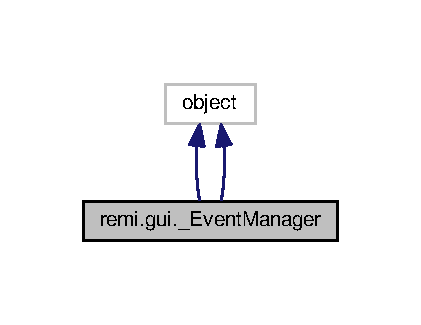
\includegraphics[width=202pt]{d2/df1/classremi_1_1gui_1_1__EventManager__inherit__graph}
\end{center}
\end{figure}


Collaboration diagram for remi.\+gui.\+\_\+\+Event\+Manager\+:
\nopagebreak
\begin{figure}[H]
\begin{center}
\leavevmode
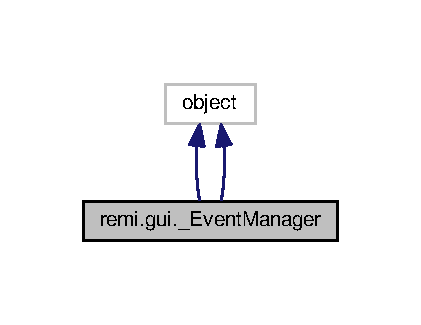
\includegraphics[width=202pt]{df/d0b/classremi_1_1gui_1_1__EventManager__coll__graph}
\end{center}
\end{figure}
\subsection*{Public Member Functions}
\begin{DoxyCompactItemize}
\item 
def \hyperlink{classremi_1_1gui_1_1__EventManager_a16be9ca73a8345abe44c9fc8593239ed}{\+\_\+\+\_\+init\+\_\+\+\_\+} (self, emitter)
\item 
def \hyperlink{classremi_1_1gui_1_1__EventManager_a586d13aa22f66990a6377a7d0b922c4e}{propagate} (self, eventname, params)
\item 
def \hyperlink{classremi_1_1gui_1_1__EventManager_a2200dc060a578b6cc9b0ac2ced29cea2}{register\+\_\+listener} (self, eventname, callback, userdata)
\item 
def \hyperlink{classremi_1_1gui_1_1__EventManager_a16be9ca73a8345abe44c9fc8593239ed}{\+\_\+\+\_\+init\+\_\+\+\_\+} (self, emitter)
\item 
def \hyperlink{classremi_1_1gui_1_1__EventManager_a586d13aa22f66990a6377a7d0b922c4e}{propagate} (self, eventname, params)
\item 
def \hyperlink{classremi_1_1gui_1_1__EventManager_a2200dc060a578b6cc9b0ac2ced29cea2}{register\+\_\+listener} (self, eventname, callback, userdata)
\end{DoxyCompactItemize}
\subsection*{Public Attributes}
\begin{DoxyCompactItemize}
\item 
{\bfseries listeners}\hypertarget{classremi_1_1gui_1_1__EventManager_adbe7ac1e7d9371d449324dd7367f4291}{}\label{classremi_1_1gui_1_1__EventManager_adbe7ac1e7d9371d449324dd7367f4291}

\item 
{\bfseries emitter}\hypertarget{classremi_1_1gui_1_1__EventManager_af5929a97e1e1cda794976de6f0b1155f}{}\label{classremi_1_1gui_1_1__EventManager_af5929a97e1e1cda794976de6f0b1155f}

\end{DoxyCompactItemize}


\subsection{Detailed Description}
\begin{DoxyVerb}Manages the event propagation to the listeners functions\end{DoxyVerb}
 

\subsection{Constructor \& Destructor Documentation}
\index{remi\+::gui\+::\+\_\+\+Event\+Manager@{remi\+::gui\+::\+\_\+\+Event\+Manager}!\+\_\+\+\_\+init\+\_\+\+\_\+@{\+\_\+\+\_\+init\+\_\+\+\_\+}}
\index{\+\_\+\+\_\+init\+\_\+\+\_\+@{\+\_\+\+\_\+init\+\_\+\+\_\+}!remi\+::gui\+::\+\_\+\+Event\+Manager@{remi\+::gui\+::\+\_\+\+Event\+Manager}}
\subsubsection[{\texorpdfstring{\+\_\+\+\_\+init\+\_\+\+\_\+(self, emitter)}{__init__(self, emitter)}}]{\setlength{\rightskip}{0pt plus 5cm}def remi.\+gui.\+\_\+\+Event\+Manager.\+\_\+\+\_\+init\+\_\+\+\_\+ (
\begin{DoxyParamCaption}
\item[{}]{self, }
\item[{}]{emitter}
\end{DoxyParamCaption}
)}\hypertarget{classremi_1_1gui_1_1__EventManager_a16be9ca73a8345abe44c9fc8593239ed}{}\label{classremi_1_1gui_1_1__EventManager_a16be9ca73a8345abe44c9fc8593239ed}
\begin{DoxyVerb}Args:
    emitter:
\end{DoxyVerb}
 \index{remi\+::gui\+::\+\_\+\+Event\+Manager@{remi\+::gui\+::\+\_\+\+Event\+Manager}!\+\_\+\+\_\+init\+\_\+\+\_\+@{\+\_\+\+\_\+init\+\_\+\+\_\+}}
\index{\+\_\+\+\_\+init\+\_\+\+\_\+@{\+\_\+\+\_\+init\+\_\+\+\_\+}!remi\+::gui\+::\+\_\+\+Event\+Manager@{remi\+::gui\+::\+\_\+\+Event\+Manager}}
\subsubsection[{\texorpdfstring{\+\_\+\+\_\+init\+\_\+\+\_\+(self, emitter)}{__init__(self, emitter)}}]{\setlength{\rightskip}{0pt plus 5cm}def remi.\+gui.\+\_\+\+Event\+Manager.\+\_\+\+\_\+init\+\_\+\+\_\+ (
\begin{DoxyParamCaption}
\item[{}]{self, }
\item[{}]{emitter}
\end{DoxyParamCaption}
)}\hypertarget{classremi_1_1gui_1_1__EventManager_a16be9ca73a8345abe44c9fc8593239ed}{}\label{classremi_1_1gui_1_1__EventManager_a16be9ca73a8345abe44c9fc8593239ed}
\begin{DoxyVerb}Args:
    emitter:
\end{DoxyVerb}
 

\subsection{Member Function Documentation}
\index{remi\+::gui\+::\+\_\+\+Event\+Manager@{remi\+::gui\+::\+\_\+\+Event\+Manager}!propagate@{propagate}}
\index{propagate@{propagate}!remi\+::gui\+::\+\_\+\+Event\+Manager@{remi\+::gui\+::\+\_\+\+Event\+Manager}}
\subsubsection[{\texorpdfstring{propagate(self, eventname, params)}{propagate(self, eventname, params)}}]{\setlength{\rightskip}{0pt plus 5cm}def remi.\+gui.\+\_\+\+Event\+Manager.\+propagate (
\begin{DoxyParamCaption}
\item[{}]{self, }
\item[{}]{eventname, }
\item[{}]{params}
\end{DoxyParamCaption}
)}\hypertarget{classremi_1_1gui_1_1__EventManager_a586d13aa22f66990a6377a7d0b922c4e}{}\label{classremi_1_1gui_1_1__EventManager_a586d13aa22f66990a6377a7d0b922c4e}
\begin{DoxyVerb}Args:
    eventname:
    params:

Returns:\end{DoxyVerb}
 \index{remi\+::gui\+::\+\_\+\+Event\+Manager@{remi\+::gui\+::\+\_\+\+Event\+Manager}!propagate@{propagate}}
\index{propagate@{propagate}!remi\+::gui\+::\+\_\+\+Event\+Manager@{remi\+::gui\+::\+\_\+\+Event\+Manager}}
\subsubsection[{\texorpdfstring{propagate(self, eventname, params)}{propagate(self, eventname, params)}}]{\setlength{\rightskip}{0pt plus 5cm}def remi.\+gui.\+\_\+\+Event\+Manager.\+propagate (
\begin{DoxyParamCaption}
\item[{}]{self, }
\item[{}]{eventname, }
\item[{}]{params}
\end{DoxyParamCaption}
)}\hypertarget{classremi_1_1gui_1_1__EventManager_a586d13aa22f66990a6377a7d0b922c4e}{}\label{classremi_1_1gui_1_1__EventManager_a586d13aa22f66990a6377a7d0b922c4e}
\begin{DoxyVerb}Args:
    eventname:
    params:

Returns:\end{DoxyVerb}
 \index{remi\+::gui\+::\+\_\+\+Event\+Manager@{remi\+::gui\+::\+\_\+\+Event\+Manager}!register\+\_\+listener@{register\+\_\+listener}}
\index{register\+\_\+listener@{register\+\_\+listener}!remi\+::gui\+::\+\_\+\+Event\+Manager@{remi\+::gui\+::\+\_\+\+Event\+Manager}}
\subsubsection[{\texorpdfstring{register\+\_\+listener(self, eventname, callback, userdata)}{register_listener(self, eventname, callback, userdata)}}]{\setlength{\rightskip}{0pt plus 5cm}def remi.\+gui.\+\_\+\+Event\+Manager.\+register\+\_\+listener (
\begin{DoxyParamCaption}
\item[{}]{self, }
\item[{}]{eventname, }
\item[{}]{callback, }
\item[{}]{userdata}
\end{DoxyParamCaption}
)}\hypertarget{classremi_1_1gui_1_1__EventManager_a2200dc060a578b6cc9b0ac2ced29cea2}{}\label{classremi_1_1gui_1_1__EventManager_a2200dc060a578b6cc9b0ac2ced29cea2}
\begin{DoxyVerb}register a listener for a specific event

Args:
    eventname (str): The event identifier, like Widget.EVENT_ONCLICK that is 'onclick'.
    callback (function): Function pointer to the callback function.
    userdata (tuple): Extra optional userdata that will be passed to the listener.
\end{DoxyVerb}
 \index{remi\+::gui\+::\+\_\+\+Event\+Manager@{remi\+::gui\+::\+\_\+\+Event\+Manager}!register\+\_\+listener@{register\+\_\+listener}}
\index{register\+\_\+listener@{register\+\_\+listener}!remi\+::gui\+::\+\_\+\+Event\+Manager@{remi\+::gui\+::\+\_\+\+Event\+Manager}}
\subsubsection[{\texorpdfstring{register\+\_\+listener(self, eventname, callback, userdata)}{register_listener(self, eventname, callback, userdata)}}]{\setlength{\rightskip}{0pt plus 5cm}def remi.\+gui.\+\_\+\+Event\+Manager.\+register\+\_\+listener (
\begin{DoxyParamCaption}
\item[{}]{self, }
\item[{}]{eventname, }
\item[{}]{callback, }
\item[{}]{userdata}
\end{DoxyParamCaption}
)}\hypertarget{classremi_1_1gui_1_1__EventManager_a2200dc060a578b6cc9b0ac2ced29cea2}{}\label{classremi_1_1gui_1_1__EventManager_a2200dc060a578b6cc9b0ac2ced29cea2}
\begin{DoxyVerb}register a listener for a specific event

Args:
    eventname (str): The event identifier, like Widget.EVENT_ONCLICK that is 'onclick'.
    callback (function): Function pointer to the callback function.
    userdata (tuple): Extra optional userdata that will be passed to the listener.
\end{DoxyVerb}
 

The documentation for this class was generated from the following file\+:\begin{DoxyCompactItemize}
\item 
Compiled/\+Server/remi/gui.\+py\end{DoxyCompactItemize}

\hypertarget{classremi_1_1gui_1_1__MixinTextualWidget}{}\section{remi.\+gui.\+\_\+\+Mixin\+Textual\+Widget Class Reference}
\label{classremi_1_1gui_1_1__MixinTextualWidget}\index{remi.\+gui.\+\_\+\+Mixin\+Textual\+Widget@{remi.\+gui.\+\_\+\+Mixin\+Textual\+Widget}}


Inheritance diagram for remi.\+gui.\+\_\+\+Mixin\+Textual\+Widget\+:
\nopagebreak
\begin{figure}[H]
\begin{center}
\leavevmode
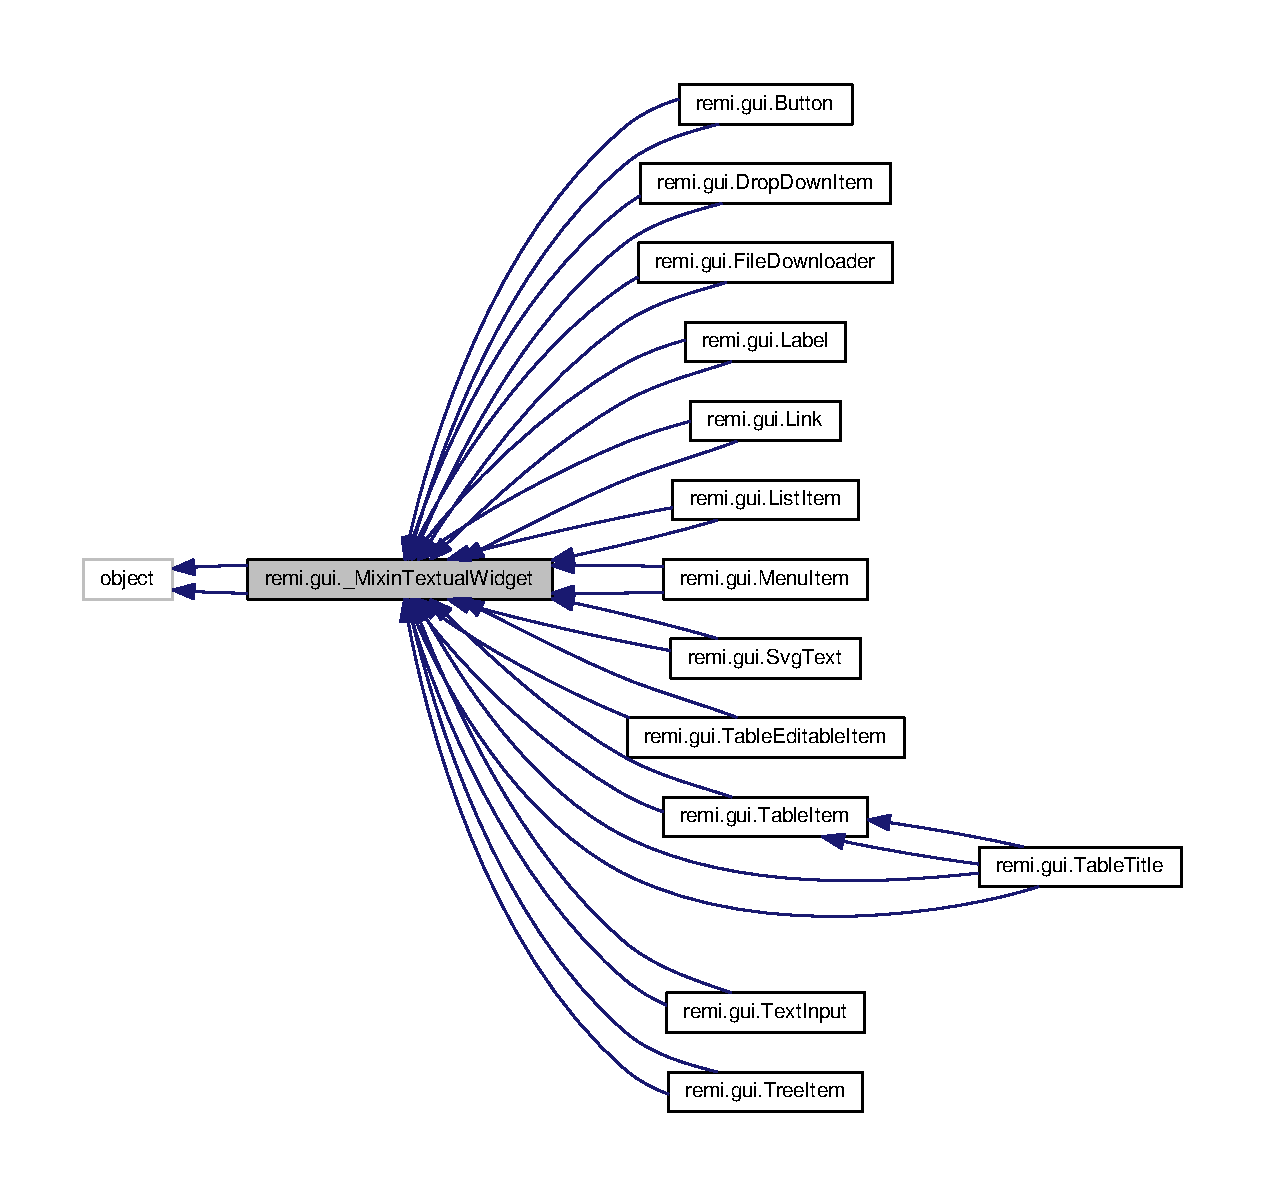
\includegraphics[width=350pt]{d1/d84/classremi_1_1gui_1_1__MixinTextualWidget__inherit__graph}
\end{center}
\end{figure}


Collaboration diagram for remi.\+gui.\+\_\+\+Mixin\+Textual\+Widget\+:
\nopagebreak
\begin{figure}[H]
\begin{center}
\leavevmode
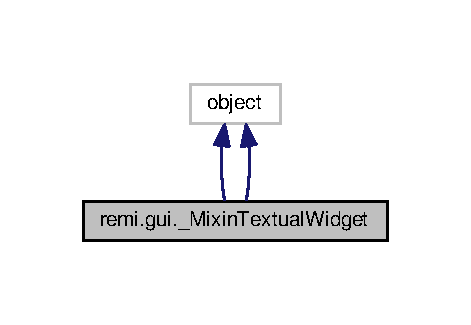
\includegraphics[width=226pt]{d8/dac/classremi_1_1gui_1_1__MixinTextualWidget__coll__graph}
\end{center}
\end{figure}
\subsection*{Public Member Functions}
\begin{DoxyCompactItemize}
\item 
def \hyperlink{classremi_1_1gui_1_1__MixinTextualWidget_af97deaf87748715de8d75616633abcc1}{set\+\_\+text} (self, text)
\item 
def \hyperlink{classremi_1_1gui_1_1__MixinTextualWidget_a45202e83618ad040ae73868f6c1aebd4}{get\+\_\+text} (self)
\item 
def \hyperlink{classremi_1_1gui_1_1__MixinTextualWidget_af97deaf87748715de8d75616633abcc1}{set\+\_\+text} (self, text)
\item 
def \hyperlink{classremi_1_1gui_1_1__MixinTextualWidget_a45202e83618ad040ae73868f6c1aebd4}{get\+\_\+text} (self)
\end{DoxyCompactItemize}


\subsection{Detailed Description}
\begin{DoxyVerb}\end{DoxyVerb}
 

\subsection{Member Function Documentation}
\index{remi\+::gui\+::\+\_\+\+Mixin\+Textual\+Widget@{remi\+::gui\+::\+\_\+\+Mixin\+Textual\+Widget}!get\+\_\+text@{get\+\_\+text}}
\index{get\+\_\+text@{get\+\_\+text}!remi\+::gui\+::\+\_\+\+Mixin\+Textual\+Widget@{remi\+::gui\+::\+\_\+\+Mixin\+Textual\+Widget}}
\subsubsection[{\texorpdfstring{get\+\_\+text(self)}{get_text(self)}}]{\setlength{\rightskip}{0pt plus 5cm}def remi.\+gui.\+\_\+\+Mixin\+Textual\+Widget.\+get\+\_\+text (
\begin{DoxyParamCaption}
\item[{}]{self}
\end{DoxyParamCaption}
)}\hypertarget{classremi_1_1gui_1_1__MixinTextualWidget_a45202e83618ad040ae73868f6c1aebd4}{}\label{classremi_1_1gui_1_1__MixinTextualWidget_a45202e83618ad040ae73868f6c1aebd4}
\begin{DoxyVerb}Returns:
    str: The text content of the Widget. You can set the text content with set_text(text).
\end{DoxyVerb}
 \index{remi\+::gui\+::\+\_\+\+Mixin\+Textual\+Widget@{remi\+::gui\+::\+\_\+\+Mixin\+Textual\+Widget}!get\+\_\+text@{get\+\_\+text}}
\index{get\+\_\+text@{get\+\_\+text}!remi\+::gui\+::\+\_\+\+Mixin\+Textual\+Widget@{remi\+::gui\+::\+\_\+\+Mixin\+Textual\+Widget}}
\subsubsection[{\texorpdfstring{get\+\_\+text(self)}{get_text(self)}}]{\setlength{\rightskip}{0pt plus 5cm}def remi.\+gui.\+\_\+\+Mixin\+Textual\+Widget.\+get\+\_\+text (
\begin{DoxyParamCaption}
\item[{}]{self}
\end{DoxyParamCaption}
)}\hypertarget{classremi_1_1gui_1_1__MixinTextualWidget_a45202e83618ad040ae73868f6c1aebd4}{}\label{classremi_1_1gui_1_1__MixinTextualWidget_a45202e83618ad040ae73868f6c1aebd4}
\begin{DoxyVerb}Returns:
    str: The text content of the Widget. You can set the text content with set_text(text).
\end{DoxyVerb}
 \index{remi\+::gui\+::\+\_\+\+Mixin\+Textual\+Widget@{remi\+::gui\+::\+\_\+\+Mixin\+Textual\+Widget}!set\+\_\+text@{set\+\_\+text}}
\index{set\+\_\+text@{set\+\_\+text}!remi\+::gui\+::\+\_\+\+Mixin\+Textual\+Widget@{remi\+::gui\+::\+\_\+\+Mixin\+Textual\+Widget}}
\subsubsection[{\texorpdfstring{set\+\_\+text(self, text)}{set_text(self, text)}}]{\setlength{\rightskip}{0pt plus 5cm}def remi.\+gui.\+\_\+\+Mixin\+Textual\+Widget.\+set\+\_\+text (
\begin{DoxyParamCaption}
\item[{}]{self, }
\item[{}]{text}
\end{DoxyParamCaption}
)}\hypertarget{classremi_1_1gui_1_1__MixinTextualWidget_af97deaf87748715de8d75616633abcc1}{}\label{classremi_1_1gui_1_1__MixinTextualWidget_af97deaf87748715de8d75616633abcc1}
\begin{DoxyVerb}Sets the text label for the Widget.

Args:
    text (str): The string label of the Widget.
\end{DoxyVerb}
 \index{remi\+::gui\+::\+\_\+\+Mixin\+Textual\+Widget@{remi\+::gui\+::\+\_\+\+Mixin\+Textual\+Widget}!set\+\_\+text@{set\+\_\+text}}
\index{set\+\_\+text@{set\+\_\+text}!remi\+::gui\+::\+\_\+\+Mixin\+Textual\+Widget@{remi\+::gui\+::\+\_\+\+Mixin\+Textual\+Widget}}
\subsubsection[{\texorpdfstring{set\+\_\+text(self, text)}{set_text(self, text)}}]{\setlength{\rightskip}{0pt plus 5cm}def remi.\+gui.\+\_\+\+Mixin\+Textual\+Widget.\+set\+\_\+text (
\begin{DoxyParamCaption}
\item[{}]{self, }
\item[{}]{text}
\end{DoxyParamCaption}
)}\hypertarget{classremi_1_1gui_1_1__MixinTextualWidget_af97deaf87748715de8d75616633abcc1}{}\label{classremi_1_1gui_1_1__MixinTextualWidget_af97deaf87748715de8d75616633abcc1}
\begin{DoxyVerb}Sets the text label for the Widget.

Args:
    text (str): The string label of the Widget.
\end{DoxyVerb}
 

The documentation for this class was generated from the following file\+:\begin{DoxyCompactItemize}
\item 
Compiled/\+Server/remi/gui.\+py\end{DoxyCompactItemize}

\hypertarget{classremi_1_1gui_1_1__SyncableValuesMixin}{}\section{remi.\+gui.\+\_\+\+Syncable\+Values\+Mixin Class Reference}
\label{classremi_1_1gui_1_1__SyncableValuesMixin}\index{remi.\+gui.\+\_\+\+Syncable\+Values\+Mixin@{remi.\+gui.\+\_\+\+Syncable\+Values\+Mixin}}


Inheritance diagram for remi.\+gui.\+\_\+\+Syncable\+Values\+Mixin\+:
\nopagebreak
\begin{figure}[H]
\begin{center}
\leavevmode
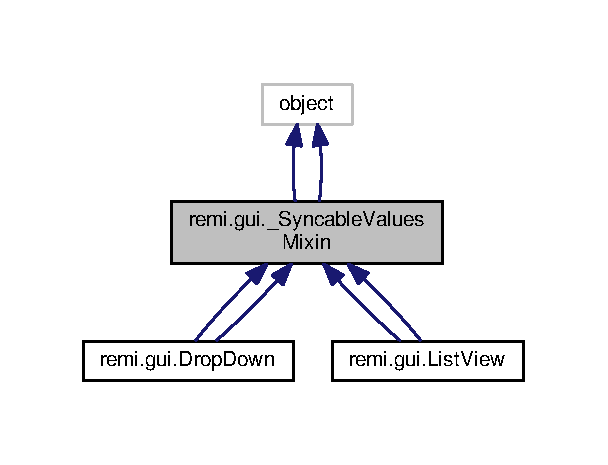
\includegraphics[width=292pt]{dd/dbe/classremi_1_1gui_1_1__SyncableValuesMixin__inherit__graph}
\end{center}
\end{figure}


Collaboration diagram for remi.\+gui.\+\_\+\+Syncable\+Values\+Mixin\+:
\nopagebreak
\begin{figure}[H]
\begin{center}
\leavevmode
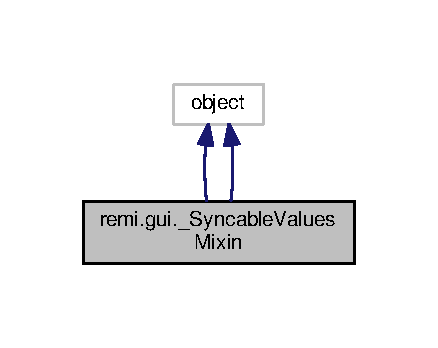
\includegraphics[width=210pt]{d9/de2/classremi_1_1gui_1_1__SyncableValuesMixin__coll__graph}
\end{center}
\end{figure}
\subsection*{Public Member Functions}
\begin{DoxyCompactItemize}
\item 
def \hyperlink{classremi_1_1gui_1_1__SyncableValuesMixin_a16cf5eabf0ddb802a0d029e656d0f11d}{synchronize\+\_\+values} (self, values)
\item 
def \hyperlink{classremi_1_1gui_1_1__SyncableValuesMixin_a16cf5eabf0ddb802a0d029e656d0f11d}{synchronize\+\_\+values} (self, values)
\end{DoxyCompactItemize}


\subsection{Detailed Description}
\begin{DoxyVerb}\end{DoxyVerb}
 

\subsection{Member Function Documentation}
\index{remi\+::gui\+::\+\_\+\+Syncable\+Values\+Mixin@{remi\+::gui\+::\+\_\+\+Syncable\+Values\+Mixin}!synchronize\+\_\+values@{synchronize\+\_\+values}}
\index{synchronize\+\_\+values@{synchronize\+\_\+values}!remi\+::gui\+::\+\_\+\+Syncable\+Values\+Mixin@{remi\+::gui\+::\+\_\+\+Syncable\+Values\+Mixin}}
\subsubsection[{\texorpdfstring{synchronize\+\_\+values(self, values)}{synchronize_values(self, values)}}]{\setlength{\rightskip}{0pt plus 5cm}def remi.\+gui.\+\_\+\+Syncable\+Values\+Mixin.\+synchronize\+\_\+values (
\begin{DoxyParamCaption}
\item[{}]{self, }
\item[{}]{values}
\end{DoxyParamCaption}
)}\hypertarget{classremi_1_1gui_1_1__SyncableValuesMixin_a16cf5eabf0ddb802a0d029e656d0f11d}{}\label{classremi_1_1gui_1_1__SyncableValuesMixin_a16cf5eabf0ddb802a0d029e656d0f11d}
\begin{DoxyVerb}Args:
    values:
\end{DoxyVerb}
 \index{remi\+::gui\+::\+\_\+\+Syncable\+Values\+Mixin@{remi\+::gui\+::\+\_\+\+Syncable\+Values\+Mixin}!synchronize\+\_\+values@{synchronize\+\_\+values}}
\index{synchronize\+\_\+values@{synchronize\+\_\+values}!remi\+::gui\+::\+\_\+\+Syncable\+Values\+Mixin@{remi\+::gui\+::\+\_\+\+Syncable\+Values\+Mixin}}
\subsubsection[{\texorpdfstring{synchronize\+\_\+values(self, values)}{synchronize_values(self, values)}}]{\setlength{\rightskip}{0pt plus 5cm}def remi.\+gui.\+\_\+\+Syncable\+Values\+Mixin.\+synchronize\+\_\+values (
\begin{DoxyParamCaption}
\item[{}]{self, }
\item[{}]{values}
\end{DoxyParamCaption}
)}\hypertarget{classremi_1_1gui_1_1__SyncableValuesMixin_a16cf5eabf0ddb802a0d029e656d0f11d}{}\label{classremi_1_1gui_1_1__SyncableValuesMixin_a16cf5eabf0ddb802a0d029e656d0f11d}
\begin{DoxyVerb}Args:
    values:
\end{DoxyVerb}
 

The documentation for this class was generated from the following file\+:\begin{DoxyCompactItemize}
\item 
Compiled/\+Server/remi/gui.\+py\end{DoxyCompactItemize}

\hypertarget{classremi_1_1server_1_1__UpdateThread}{}\section{remi.\+server.\+\_\+\+Update\+Thread Class Reference}
\label{classremi_1_1server_1_1__UpdateThread}\index{remi.\+server.\+\_\+\+Update\+Thread@{remi.\+server.\+\_\+\+Update\+Thread}}


Inheritance diagram for remi.\+server.\+\_\+\+Update\+Thread\+:
\nopagebreak
\begin{figure}[H]
\begin{center}
\leavevmode
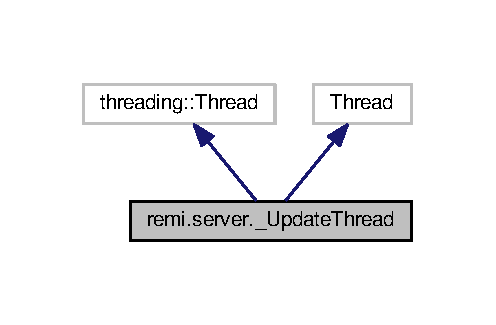
\includegraphics[width=238pt]{d5/d64/classremi_1_1server_1_1__UpdateThread__inherit__graph}
\end{center}
\end{figure}


Collaboration diagram for remi.\+server.\+\_\+\+Update\+Thread\+:
\nopagebreak
\begin{figure}[H]
\begin{center}
\leavevmode
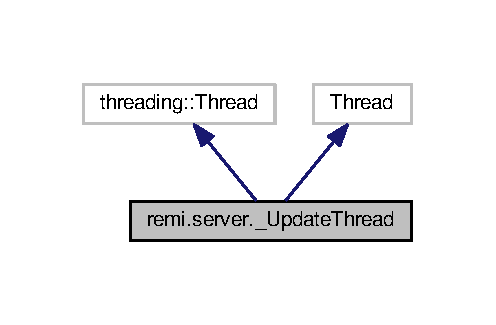
\includegraphics[width=238pt]{d3/d9a/classremi_1_1server_1_1__UpdateThread__coll__graph}
\end{center}
\end{figure}
\subsection*{Public Member Functions}
\begin{DoxyCompactItemize}
\item 
def \hyperlink{classremi_1_1server_1_1__UpdateThread_a4a2ff6537d731731db9d6eba47713cd7}{\+\_\+\+\_\+init\+\_\+\+\_\+} (self, interval)
\item 
def \hyperlink{classremi_1_1server_1_1__UpdateThread_a1894523d28dadfbc4d5b3be38756b5e0}{stop} (self)
\item 
def \hyperlink{classremi_1_1server_1_1__UpdateThread_adf29050ba815d4d441aeddc3475de39c}{run} (self)
\item 
def \hyperlink{classremi_1_1server_1_1__UpdateThread_a4a2ff6537d731731db9d6eba47713cd7}{\+\_\+\+\_\+init\+\_\+\+\_\+} (self, interval)
\item 
def \hyperlink{classremi_1_1server_1_1__UpdateThread_a1894523d28dadfbc4d5b3be38756b5e0}{stop} (self)
\item 
def \hyperlink{classremi_1_1server_1_1__UpdateThread_adf29050ba815d4d441aeddc3475de39c}{run} (self)
\end{DoxyCompactItemize}
\subsection*{Public Attributes}
\begin{DoxyCompactItemize}
\item 
{\bfseries daemon}\hypertarget{classremi_1_1server_1_1__UpdateThread_abe936c52d1fd19bde98a3a6c5a0d42f7}{}\label{classremi_1_1server_1_1__UpdateThread_abe936c52d1fd19bde98a3a6c5a0d42f7}

\end{DoxyCompactItemize}
\subsection*{Static Public Attributes}
\begin{DoxyCompactItemize}
\item 
bool {\bfseries daemon} = True\hypertarget{classremi_1_1server_1_1__UpdateThread_a8d6ec40d1f386283ab1c8de59711ec16}{}\label{classremi_1_1server_1_1__UpdateThread_a8d6ec40d1f386283ab1c8de59711ec16}

\end{DoxyCompactItemize}


\subsection{Detailed Description}
\begin{DoxyVerb}\end{DoxyVerb}
 

\subsection{Constructor \& Destructor Documentation}
\index{remi\+::server\+::\+\_\+\+Update\+Thread@{remi\+::server\+::\+\_\+\+Update\+Thread}!\+\_\+\+\_\+init\+\_\+\+\_\+@{\+\_\+\+\_\+init\+\_\+\+\_\+}}
\index{\+\_\+\+\_\+init\+\_\+\+\_\+@{\+\_\+\+\_\+init\+\_\+\+\_\+}!remi\+::server\+::\+\_\+\+Update\+Thread@{remi\+::server\+::\+\_\+\+Update\+Thread}}
\subsubsection[{\texorpdfstring{\+\_\+\+\_\+init\+\_\+\+\_\+(self, interval)}{__init__(self, interval)}}]{\setlength{\rightskip}{0pt plus 5cm}def remi.\+server.\+\_\+\+Update\+Thread.\+\_\+\+\_\+init\+\_\+\+\_\+ (
\begin{DoxyParamCaption}
\item[{}]{self, }
\item[{}]{interval}
\end{DoxyParamCaption}
)}\hypertarget{classremi_1_1server_1_1__UpdateThread_a4a2ff6537d731731db9d6eba47713cd7}{}\label{classremi_1_1server_1_1__UpdateThread_a4a2ff6537d731731db9d6eba47713cd7}
\begin{DoxyVerb}Args:
    interval:
\end{DoxyVerb}
 \index{remi\+::server\+::\+\_\+\+Update\+Thread@{remi\+::server\+::\+\_\+\+Update\+Thread}!\+\_\+\+\_\+init\+\_\+\+\_\+@{\+\_\+\+\_\+init\+\_\+\+\_\+}}
\index{\+\_\+\+\_\+init\+\_\+\+\_\+@{\+\_\+\+\_\+init\+\_\+\+\_\+}!remi\+::server\+::\+\_\+\+Update\+Thread@{remi\+::server\+::\+\_\+\+Update\+Thread}}
\subsubsection[{\texorpdfstring{\+\_\+\+\_\+init\+\_\+\+\_\+(self, interval)}{__init__(self, interval)}}]{\setlength{\rightskip}{0pt plus 5cm}def remi.\+server.\+\_\+\+Update\+Thread.\+\_\+\+\_\+init\+\_\+\+\_\+ (
\begin{DoxyParamCaption}
\item[{}]{self, }
\item[{}]{interval}
\end{DoxyParamCaption}
)}\hypertarget{classremi_1_1server_1_1__UpdateThread_a4a2ff6537d731731db9d6eba47713cd7}{}\label{classremi_1_1server_1_1__UpdateThread_a4a2ff6537d731731db9d6eba47713cd7}
\begin{DoxyVerb}Args:
    interval:
\end{DoxyVerb}
 

\subsection{Member Function Documentation}
\index{remi\+::server\+::\+\_\+\+Update\+Thread@{remi\+::server\+::\+\_\+\+Update\+Thread}!run@{run}}
\index{run@{run}!remi\+::server\+::\+\_\+\+Update\+Thread@{remi\+::server\+::\+\_\+\+Update\+Thread}}
\subsubsection[{\texorpdfstring{run(self)}{run(self)}}]{\setlength{\rightskip}{0pt plus 5cm}def remi.\+server.\+\_\+\+Update\+Thread.\+run (
\begin{DoxyParamCaption}
\item[{}]{self}
\end{DoxyParamCaption}
)}\hypertarget{classremi_1_1server_1_1__UpdateThread_adf29050ba815d4d441aeddc3475de39c}{}\label{classremi_1_1server_1_1__UpdateThread_adf29050ba815d4d441aeddc3475de39c}
\begin{DoxyVerb}\end{DoxyVerb}
 \index{remi\+::server\+::\+\_\+\+Update\+Thread@{remi\+::server\+::\+\_\+\+Update\+Thread}!run@{run}}
\index{run@{run}!remi\+::server\+::\+\_\+\+Update\+Thread@{remi\+::server\+::\+\_\+\+Update\+Thread}}
\subsubsection[{\texorpdfstring{run(self)}{run(self)}}]{\setlength{\rightskip}{0pt plus 5cm}def remi.\+server.\+\_\+\+Update\+Thread.\+run (
\begin{DoxyParamCaption}
\item[{}]{self}
\end{DoxyParamCaption}
)}\hypertarget{classremi_1_1server_1_1__UpdateThread_adf29050ba815d4d441aeddc3475de39c}{}\label{classremi_1_1server_1_1__UpdateThread_adf29050ba815d4d441aeddc3475de39c}
\begin{DoxyVerb}\end{DoxyVerb}
 \index{remi\+::server\+::\+\_\+\+Update\+Thread@{remi\+::server\+::\+\_\+\+Update\+Thread}!stop@{stop}}
\index{stop@{stop}!remi\+::server\+::\+\_\+\+Update\+Thread@{remi\+::server\+::\+\_\+\+Update\+Thread}}
\subsubsection[{\texorpdfstring{stop(self)}{stop(self)}}]{\setlength{\rightskip}{0pt plus 5cm}def remi.\+server.\+\_\+\+Update\+Thread.\+stop (
\begin{DoxyParamCaption}
\item[{}]{self}
\end{DoxyParamCaption}
)}\hypertarget{classremi_1_1server_1_1__UpdateThread_a1894523d28dadfbc4d5b3be38756b5e0}{}\label{classremi_1_1server_1_1__UpdateThread_a1894523d28dadfbc4d5b3be38756b5e0}
\begin{DoxyVerb}\end{DoxyVerb}
 \index{remi\+::server\+::\+\_\+\+Update\+Thread@{remi\+::server\+::\+\_\+\+Update\+Thread}!stop@{stop}}
\index{stop@{stop}!remi\+::server\+::\+\_\+\+Update\+Thread@{remi\+::server\+::\+\_\+\+Update\+Thread}}
\subsubsection[{\texorpdfstring{stop(self)}{stop(self)}}]{\setlength{\rightskip}{0pt plus 5cm}def remi.\+server.\+\_\+\+Update\+Thread.\+stop (
\begin{DoxyParamCaption}
\item[{}]{self}
\end{DoxyParamCaption}
)}\hypertarget{classremi_1_1server_1_1__UpdateThread_a1894523d28dadfbc4d5b3be38756b5e0}{}\label{classremi_1_1server_1_1__UpdateThread_a1894523d28dadfbc4d5b3be38756b5e0}
\begin{DoxyVerb}\end{DoxyVerb}
 

The documentation for this class was generated from the following file\+:\begin{DoxyCompactItemize}
\item 
Compiled/\+Server/remi/server.\+py\end{DoxyCompactItemize}

\hypertarget{classremi_1_1gui_1_1__VersionedDictionary}{}\section{remi.\+gui.\+\_\+\+Versioned\+Dictionary Class Reference}
\label{classremi_1_1gui_1_1__VersionedDictionary}\index{remi.\+gui.\+\_\+\+Versioned\+Dictionary@{remi.\+gui.\+\_\+\+Versioned\+Dictionary}}


Inheritance diagram for remi.\+gui.\+\_\+\+Versioned\+Dictionary\+:
\nopagebreak
\begin{figure}[H]
\begin{center}
\leavevmode
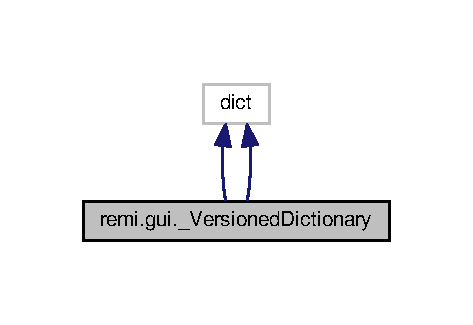
\includegraphics[width=227pt]{d0/df1/classremi_1_1gui_1_1__VersionedDictionary__inherit__graph}
\end{center}
\end{figure}


Collaboration diagram for remi.\+gui.\+\_\+\+Versioned\+Dictionary\+:
\nopagebreak
\begin{figure}[H]
\begin{center}
\leavevmode
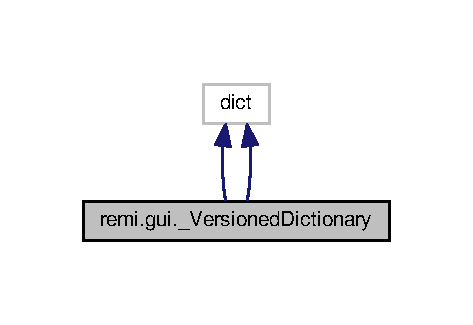
\includegraphics[width=227pt]{d8/d9f/classremi_1_1gui_1_1__VersionedDictionary__coll__graph}
\end{center}
\end{figure}
\subsection*{Public Member Functions}
\begin{DoxyCompactItemize}
\item 
def \hyperlink{classremi_1_1gui_1_1__VersionedDictionary_a368090f9fb719664910474f128a00948}{\+\_\+\+\_\+init\+\_\+\+\_\+} (self, args, kwargs)
\item 
def \hyperlink{classremi_1_1gui_1_1__VersionedDictionary_a7d6e0439fc9588d469cf39c4b1b37e29}{\+\_\+\+\_\+setitem\+\_\+\+\_\+} (self, key, value, version\+\_\+increment=1)
\item 
def \hyperlink{classremi_1_1gui_1_1__VersionedDictionary_a05cbb94364218c8156c57418f2fdabf5}{\+\_\+\+\_\+delitem\+\_\+\+\_\+} (self, key, version\+\_\+increment=1)
\item 
def \hyperlink{classremi_1_1gui_1_1__VersionedDictionary_a909eb28346814808e5054d31fb0e2e9a}{pop} (self, key, d=None, version\+\_\+increment=1)
\item 
def \hyperlink{classremi_1_1gui_1_1__VersionedDictionary_a113edc6da20e8dfc509242cb36d1a452}{clear} (self, version\+\_\+increment=1)
\item 
def \hyperlink{classremi_1_1gui_1_1__VersionedDictionary_afd97a72c323df62e15281ebc92be2077}{ischanged} (self)
\item 
def \hyperlink{classremi_1_1gui_1_1__VersionedDictionary_a43182b9aeea82c60b2246329cc59ae54}{align\+\_\+version} (self)
\item 
def \hyperlink{classremi_1_1gui_1_1__VersionedDictionary_a368090f9fb719664910474f128a00948}{\+\_\+\+\_\+init\+\_\+\+\_\+} (self, args, kwargs)
\item 
def \hyperlink{classremi_1_1gui_1_1__VersionedDictionary_a7d6e0439fc9588d469cf39c4b1b37e29}{\+\_\+\+\_\+setitem\+\_\+\+\_\+} (self, key, value, version\+\_\+increment=1)
\item 
def \hyperlink{classremi_1_1gui_1_1__VersionedDictionary_a05cbb94364218c8156c57418f2fdabf5}{\+\_\+\+\_\+delitem\+\_\+\+\_\+} (self, key, version\+\_\+increment=1)
\item 
def \hyperlink{classremi_1_1gui_1_1__VersionedDictionary_a909eb28346814808e5054d31fb0e2e9a}{pop} (self, key, d=None, version\+\_\+increment=1)
\item 
def \hyperlink{classremi_1_1gui_1_1__VersionedDictionary_a113edc6da20e8dfc509242cb36d1a452}{clear} (self, version\+\_\+increment=1)
\item 
def \hyperlink{classremi_1_1gui_1_1__VersionedDictionary_afd97a72c323df62e15281ebc92be2077}{ischanged} (self)
\item 
def \hyperlink{classremi_1_1gui_1_1__VersionedDictionary_a43182b9aeea82c60b2246329cc59ae54}{align\+\_\+version} (self)
\end{DoxyCompactItemize}


\subsection{Detailed Description}
\begin{DoxyVerb}This dictionary allows to check if its content is changed.
   It has an attribute __version__ of type int that increments every change
\end{DoxyVerb}
 

\subsection{Constructor \& Destructor Documentation}
\index{remi\+::gui\+::\+\_\+\+Versioned\+Dictionary@{remi\+::gui\+::\+\_\+\+Versioned\+Dictionary}!\+\_\+\+\_\+init\+\_\+\+\_\+@{\+\_\+\+\_\+init\+\_\+\+\_\+}}
\index{\+\_\+\+\_\+init\+\_\+\+\_\+@{\+\_\+\+\_\+init\+\_\+\+\_\+}!remi\+::gui\+::\+\_\+\+Versioned\+Dictionary@{remi\+::gui\+::\+\_\+\+Versioned\+Dictionary}}
\subsubsection[{\texorpdfstring{\+\_\+\+\_\+init\+\_\+\+\_\+(self, args, kwargs)}{__init__(self, args, kwargs)}}]{\setlength{\rightskip}{0pt plus 5cm}def remi.\+gui.\+\_\+\+Versioned\+Dictionary.\+\_\+\+\_\+init\+\_\+\+\_\+ (
\begin{DoxyParamCaption}
\item[{}]{self, }
\item[{}]{args, }
\item[{}]{kwargs}
\end{DoxyParamCaption}
)}\hypertarget{classremi_1_1gui_1_1__VersionedDictionary_a368090f9fb719664910474f128a00948}{}\label{classremi_1_1gui_1_1__VersionedDictionary_a368090f9fb719664910474f128a00948}
\begin{DoxyVerb}Args:
    args:
    kwargs:
\end{DoxyVerb}
 \index{remi\+::gui\+::\+\_\+\+Versioned\+Dictionary@{remi\+::gui\+::\+\_\+\+Versioned\+Dictionary}!\+\_\+\+\_\+init\+\_\+\+\_\+@{\+\_\+\+\_\+init\+\_\+\+\_\+}}
\index{\+\_\+\+\_\+init\+\_\+\+\_\+@{\+\_\+\+\_\+init\+\_\+\+\_\+}!remi\+::gui\+::\+\_\+\+Versioned\+Dictionary@{remi\+::gui\+::\+\_\+\+Versioned\+Dictionary}}
\subsubsection[{\texorpdfstring{\+\_\+\+\_\+init\+\_\+\+\_\+(self, args, kwargs)}{__init__(self, args, kwargs)}}]{\setlength{\rightskip}{0pt plus 5cm}def remi.\+gui.\+\_\+\+Versioned\+Dictionary.\+\_\+\+\_\+init\+\_\+\+\_\+ (
\begin{DoxyParamCaption}
\item[{}]{self, }
\item[{}]{args, }
\item[{}]{kwargs}
\end{DoxyParamCaption}
)}\hypertarget{classremi_1_1gui_1_1__VersionedDictionary_a368090f9fb719664910474f128a00948}{}\label{classremi_1_1gui_1_1__VersionedDictionary_a368090f9fb719664910474f128a00948}
\begin{DoxyVerb}Args:
    args:
    kwargs:
\end{DoxyVerb}
 

\subsection{Member Function Documentation}
\index{remi\+::gui\+::\+\_\+\+Versioned\+Dictionary@{remi\+::gui\+::\+\_\+\+Versioned\+Dictionary}!\+\_\+\+\_\+delitem\+\_\+\+\_\+@{\+\_\+\+\_\+delitem\+\_\+\+\_\+}}
\index{\+\_\+\+\_\+delitem\+\_\+\+\_\+@{\+\_\+\+\_\+delitem\+\_\+\+\_\+}!remi\+::gui\+::\+\_\+\+Versioned\+Dictionary@{remi\+::gui\+::\+\_\+\+Versioned\+Dictionary}}
\subsubsection[{\texorpdfstring{\+\_\+\+\_\+delitem\+\_\+\+\_\+(self, key, version\+\_\+increment=1)}{__delitem__(self, key, version_increment=1)}}]{\setlength{\rightskip}{0pt plus 5cm}def remi.\+gui.\+\_\+\+Versioned\+Dictionary.\+\_\+\+\_\+delitem\+\_\+\+\_\+ (
\begin{DoxyParamCaption}
\item[{}]{self, }
\item[{}]{key, }
\item[{}]{version\+\_\+increment = {\ttfamily 1}}
\end{DoxyParamCaption}
)}\hypertarget{classremi_1_1gui_1_1__VersionedDictionary_a05cbb94364218c8156c57418f2fdabf5}{}\label{classremi_1_1gui_1_1__VersionedDictionary_a05cbb94364218c8156c57418f2fdabf5}
\begin{DoxyVerb}Args:
    key:
    version_increment:

Returns:\end{DoxyVerb}
 \index{remi\+::gui\+::\+\_\+\+Versioned\+Dictionary@{remi\+::gui\+::\+\_\+\+Versioned\+Dictionary}!\+\_\+\+\_\+delitem\+\_\+\+\_\+@{\+\_\+\+\_\+delitem\+\_\+\+\_\+}}
\index{\+\_\+\+\_\+delitem\+\_\+\+\_\+@{\+\_\+\+\_\+delitem\+\_\+\+\_\+}!remi\+::gui\+::\+\_\+\+Versioned\+Dictionary@{remi\+::gui\+::\+\_\+\+Versioned\+Dictionary}}
\subsubsection[{\texorpdfstring{\+\_\+\+\_\+delitem\+\_\+\+\_\+(self, key, version\+\_\+increment=1)}{__delitem__(self, key, version_increment=1)}}]{\setlength{\rightskip}{0pt plus 5cm}def remi.\+gui.\+\_\+\+Versioned\+Dictionary.\+\_\+\+\_\+delitem\+\_\+\+\_\+ (
\begin{DoxyParamCaption}
\item[{}]{self, }
\item[{}]{key, }
\item[{}]{version\+\_\+increment = {\ttfamily 1}}
\end{DoxyParamCaption}
)}\hypertarget{classremi_1_1gui_1_1__VersionedDictionary_a05cbb94364218c8156c57418f2fdabf5}{}\label{classremi_1_1gui_1_1__VersionedDictionary_a05cbb94364218c8156c57418f2fdabf5}
\begin{DoxyVerb}Args:
    key:
    version_increment:

Returns:\end{DoxyVerb}
 \index{remi\+::gui\+::\+\_\+\+Versioned\+Dictionary@{remi\+::gui\+::\+\_\+\+Versioned\+Dictionary}!\+\_\+\+\_\+setitem\+\_\+\+\_\+@{\+\_\+\+\_\+setitem\+\_\+\+\_\+}}
\index{\+\_\+\+\_\+setitem\+\_\+\+\_\+@{\+\_\+\+\_\+setitem\+\_\+\+\_\+}!remi\+::gui\+::\+\_\+\+Versioned\+Dictionary@{remi\+::gui\+::\+\_\+\+Versioned\+Dictionary}}
\subsubsection[{\texorpdfstring{\+\_\+\+\_\+setitem\+\_\+\+\_\+(self, key, value, version\+\_\+increment=1)}{__setitem__(self, key, value, version_increment=1)}}]{\setlength{\rightskip}{0pt plus 5cm}def remi.\+gui.\+\_\+\+Versioned\+Dictionary.\+\_\+\+\_\+setitem\+\_\+\+\_\+ (
\begin{DoxyParamCaption}
\item[{}]{self, }
\item[{}]{key, }
\item[{}]{value, }
\item[{}]{version\+\_\+increment = {\ttfamily 1}}
\end{DoxyParamCaption}
)}\hypertarget{classremi_1_1gui_1_1__VersionedDictionary_a7d6e0439fc9588d469cf39c4b1b37e29}{}\label{classremi_1_1gui_1_1__VersionedDictionary_a7d6e0439fc9588d469cf39c4b1b37e29}
\begin{DoxyVerb}Args:
    key:
    value:
    version_increment:

Returns:\end{DoxyVerb}
 \index{remi\+::gui\+::\+\_\+\+Versioned\+Dictionary@{remi\+::gui\+::\+\_\+\+Versioned\+Dictionary}!\+\_\+\+\_\+setitem\+\_\+\+\_\+@{\+\_\+\+\_\+setitem\+\_\+\+\_\+}}
\index{\+\_\+\+\_\+setitem\+\_\+\+\_\+@{\+\_\+\+\_\+setitem\+\_\+\+\_\+}!remi\+::gui\+::\+\_\+\+Versioned\+Dictionary@{remi\+::gui\+::\+\_\+\+Versioned\+Dictionary}}
\subsubsection[{\texorpdfstring{\+\_\+\+\_\+setitem\+\_\+\+\_\+(self, key, value, version\+\_\+increment=1)}{__setitem__(self, key, value, version_increment=1)}}]{\setlength{\rightskip}{0pt plus 5cm}def remi.\+gui.\+\_\+\+Versioned\+Dictionary.\+\_\+\+\_\+setitem\+\_\+\+\_\+ (
\begin{DoxyParamCaption}
\item[{}]{self, }
\item[{}]{key, }
\item[{}]{value, }
\item[{}]{version\+\_\+increment = {\ttfamily 1}}
\end{DoxyParamCaption}
)}\hypertarget{classremi_1_1gui_1_1__VersionedDictionary_a7d6e0439fc9588d469cf39c4b1b37e29}{}\label{classremi_1_1gui_1_1__VersionedDictionary_a7d6e0439fc9588d469cf39c4b1b37e29}
\begin{DoxyVerb}Args:
    key:
    value:
    version_increment:

Returns:\end{DoxyVerb}
 \index{remi\+::gui\+::\+\_\+\+Versioned\+Dictionary@{remi\+::gui\+::\+\_\+\+Versioned\+Dictionary}!align\+\_\+version@{align\+\_\+version}}
\index{align\+\_\+version@{align\+\_\+version}!remi\+::gui\+::\+\_\+\+Versioned\+Dictionary@{remi\+::gui\+::\+\_\+\+Versioned\+Dictionary}}
\subsubsection[{\texorpdfstring{align\+\_\+version(self)}{align_version(self)}}]{\setlength{\rightskip}{0pt plus 5cm}def remi.\+gui.\+\_\+\+Versioned\+Dictionary.\+align\+\_\+version (
\begin{DoxyParamCaption}
\item[{}]{self}
\end{DoxyParamCaption}
)}\hypertarget{classremi_1_1gui_1_1__VersionedDictionary_a43182b9aeea82c60b2246329cc59ae54}{}\label{classremi_1_1gui_1_1__VersionedDictionary_a43182b9aeea82c60b2246329cc59ae54}
\begin{DoxyVerb}\end{DoxyVerb}
 \index{remi\+::gui\+::\+\_\+\+Versioned\+Dictionary@{remi\+::gui\+::\+\_\+\+Versioned\+Dictionary}!align\+\_\+version@{align\+\_\+version}}
\index{align\+\_\+version@{align\+\_\+version}!remi\+::gui\+::\+\_\+\+Versioned\+Dictionary@{remi\+::gui\+::\+\_\+\+Versioned\+Dictionary}}
\subsubsection[{\texorpdfstring{align\+\_\+version(self)}{align_version(self)}}]{\setlength{\rightskip}{0pt plus 5cm}def remi.\+gui.\+\_\+\+Versioned\+Dictionary.\+align\+\_\+version (
\begin{DoxyParamCaption}
\item[{}]{self}
\end{DoxyParamCaption}
)}\hypertarget{classremi_1_1gui_1_1__VersionedDictionary_a43182b9aeea82c60b2246329cc59ae54}{}\label{classremi_1_1gui_1_1__VersionedDictionary_a43182b9aeea82c60b2246329cc59ae54}
\begin{DoxyVerb}\end{DoxyVerb}
 \index{remi\+::gui\+::\+\_\+\+Versioned\+Dictionary@{remi\+::gui\+::\+\_\+\+Versioned\+Dictionary}!clear@{clear}}
\index{clear@{clear}!remi\+::gui\+::\+\_\+\+Versioned\+Dictionary@{remi\+::gui\+::\+\_\+\+Versioned\+Dictionary}}
\subsubsection[{\texorpdfstring{clear(self, version\+\_\+increment=1)}{clear(self, version_increment=1)}}]{\setlength{\rightskip}{0pt plus 5cm}def remi.\+gui.\+\_\+\+Versioned\+Dictionary.\+clear (
\begin{DoxyParamCaption}
\item[{}]{self, }
\item[{}]{version\+\_\+increment = {\ttfamily 1}}
\end{DoxyParamCaption}
)}\hypertarget{classremi_1_1gui_1_1__VersionedDictionary_a113edc6da20e8dfc509242cb36d1a452}{}\label{classremi_1_1gui_1_1__VersionedDictionary_a113edc6da20e8dfc509242cb36d1a452}
\begin{DoxyVerb}Args:
    version_increment:

Returns:\end{DoxyVerb}
 \index{remi\+::gui\+::\+\_\+\+Versioned\+Dictionary@{remi\+::gui\+::\+\_\+\+Versioned\+Dictionary}!clear@{clear}}
\index{clear@{clear}!remi\+::gui\+::\+\_\+\+Versioned\+Dictionary@{remi\+::gui\+::\+\_\+\+Versioned\+Dictionary}}
\subsubsection[{\texorpdfstring{clear(self, version\+\_\+increment=1)}{clear(self, version_increment=1)}}]{\setlength{\rightskip}{0pt plus 5cm}def remi.\+gui.\+\_\+\+Versioned\+Dictionary.\+clear (
\begin{DoxyParamCaption}
\item[{}]{self, }
\item[{}]{version\+\_\+increment = {\ttfamily 1}}
\end{DoxyParamCaption}
)}\hypertarget{classremi_1_1gui_1_1__VersionedDictionary_a113edc6da20e8dfc509242cb36d1a452}{}\label{classremi_1_1gui_1_1__VersionedDictionary_a113edc6da20e8dfc509242cb36d1a452}
\begin{DoxyVerb}Args:
    version_increment:

Returns:\end{DoxyVerb}
 \index{remi\+::gui\+::\+\_\+\+Versioned\+Dictionary@{remi\+::gui\+::\+\_\+\+Versioned\+Dictionary}!ischanged@{ischanged}}
\index{ischanged@{ischanged}!remi\+::gui\+::\+\_\+\+Versioned\+Dictionary@{remi\+::gui\+::\+\_\+\+Versioned\+Dictionary}}
\subsubsection[{\texorpdfstring{ischanged(self)}{ischanged(self)}}]{\setlength{\rightskip}{0pt plus 5cm}def remi.\+gui.\+\_\+\+Versioned\+Dictionary.\+ischanged (
\begin{DoxyParamCaption}
\item[{}]{self}
\end{DoxyParamCaption}
)}\hypertarget{classremi_1_1gui_1_1__VersionedDictionary_afd97a72c323df62e15281ebc92be2077}{}\label{classremi_1_1gui_1_1__VersionedDictionary_afd97a72c323df62e15281ebc92be2077}
\begin{DoxyVerb}Returns:\end{DoxyVerb}
 \index{remi\+::gui\+::\+\_\+\+Versioned\+Dictionary@{remi\+::gui\+::\+\_\+\+Versioned\+Dictionary}!ischanged@{ischanged}}
\index{ischanged@{ischanged}!remi\+::gui\+::\+\_\+\+Versioned\+Dictionary@{remi\+::gui\+::\+\_\+\+Versioned\+Dictionary}}
\subsubsection[{\texorpdfstring{ischanged(self)}{ischanged(self)}}]{\setlength{\rightskip}{0pt plus 5cm}def remi.\+gui.\+\_\+\+Versioned\+Dictionary.\+ischanged (
\begin{DoxyParamCaption}
\item[{}]{self}
\end{DoxyParamCaption}
)}\hypertarget{classremi_1_1gui_1_1__VersionedDictionary_afd97a72c323df62e15281ebc92be2077}{}\label{classremi_1_1gui_1_1__VersionedDictionary_afd97a72c323df62e15281ebc92be2077}
\begin{DoxyVerb}Returns:\end{DoxyVerb}
 \index{remi\+::gui\+::\+\_\+\+Versioned\+Dictionary@{remi\+::gui\+::\+\_\+\+Versioned\+Dictionary}!pop@{pop}}
\index{pop@{pop}!remi\+::gui\+::\+\_\+\+Versioned\+Dictionary@{remi\+::gui\+::\+\_\+\+Versioned\+Dictionary}}
\subsubsection[{\texorpdfstring{pop(self, key, d=\+None, version\+\_\+increment=1)}{pop(self, key, d=None, version_increment=1)}}]{\setlength{\rightskip}{0pt plus 5cm}def remi.\+gui.\+\_\+\+Versioned\+Dictionary.\+pop (
\begin{DoxyParamCaption}
\item[{}]{self, }
\item[{}]{key, }
\item[{}]{d = {\ttfamily None}, }
\item[{}]{version\+\_\+increment = {\ttfamily 1}}
\end{DoxyParamCaption}
)}\hypertarget{classremi_1_1gui_1_1__VersionedDictionary_a909eb28346814808e5054d31fb0e2e9a}{}\label{classremi_1_1gui_1_1__VersionedDictionary_a909eb28346814808e5054d31fb0e2e9a}
\begin{DoxyVerb}Args:
    key:
    d:
    version_increment:

Returns:\end{DoxyVerb}
 \index{remi\+::gui\+::\+\_\+\+Versioned\+Dictionary@{remi\+::gui\+::\+\_\+\+Versioned\+Dictionary}!pop@{pop}}
\index{pop@{pop}!remi\+::gui\+::\+\_\+\+Versioned\+Dictionary@{remi\+::gui\+::\+\_\+\+Versioned\+Dictionary}}
\subsubsection[{\texorpdfstring{pop(self, key, d=\+None, version\+\_\+increment=1)}{pop(self, key, d=None, version_increment=1)}}]{\setlength{\rightskip}{0pt plus 5cm}def remi.\+gui.\+\_\+\+Versioned\+Dictionary.\+pop (
\begin{DoxyParamCaption}
\item[{}]{self, }
\item[{}]{key, }
\item[{}]{d = {\ttfamily None}, }
\item[{}]{version\+\_\+increment = {\ttfamily 1}}
\end{DoxyParamCaption}
)}\hypertarget{classremi_1_1gui_1_1__VersionedDictionary_a909eb28346814808e5054d31fb0e2e9a}{}\label{classremi_1_1gui_1_1__VersionedDictionary_a909eb28346814808e5054d31fb0e2e9a}
\begin{DoxyVerb}Args:
    key:
    d:
    version_increment:

Returns:\end{DoxyVerb}
 

The documentation for this class was generated from the following file\+:\begin{DoxyCompactItemize}
\item 
Compiled/\+Server/remi/gui.\+py\end{DoxyCompactItemize}

\hypertarget{classremi_1_1server_1_1App}{}\section{remi.\+server.\+App Class Reference}
\label{classremi_1_1server_1_1App}\index{remi.\+server.\+App@{remi.\+server.\+App}}


Inheritance diagram for remi.\+server.\+App\+:
\nopagebreak
\begin{figure}[H]
\begin{center}
\leavevmode
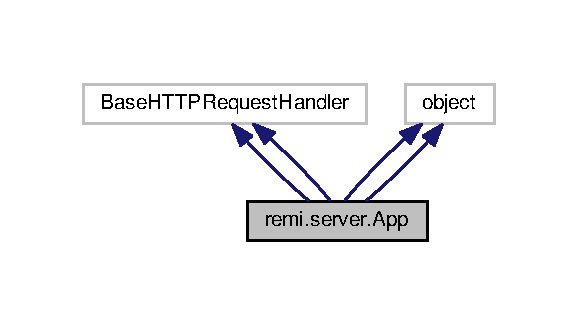
\includegraphics[width=278pt]{d4/d5f/classremi_1_1server_1_1App__inherit__graph}
\end{center}
\end{figure}


Collaboration diagram for remi.\+server.\+App\+:
\nopagebreak
\begin{figure}[H]
\begin{center}
\leavevmode
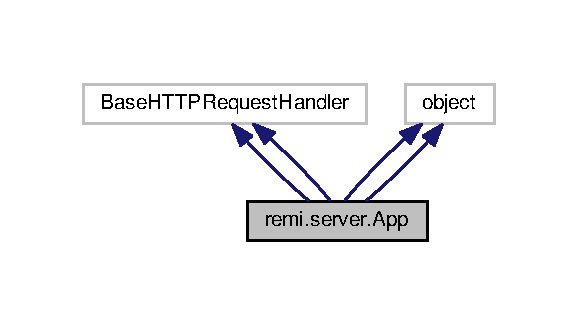
\includegraphics[width=278pt]{db/d9a/classremi_1_1server_1_1App__coll__graph}
\end{center}
\end{figure}
\subsection*{Public Member Functions}
\begin{DoxyCompactItemize}
\item 
def \hyperlink{classremi_1_1server_1_1App_a5ed1b85fb59b973897ac43ac091809cc}{\+\_\+\+\_\+init\+\_\+\+\_\+} (self, request, client\+\_\+address, server, app\+\_\+args)
\item 
def \hyperlink{classremi_1_1server_1_1App_a2be308eef6fc7edbac1f466a785f770f}{log\+\_\+message} (self, format\+\_\+string, args)
\item 
def \hyperlink{classremi_1_1server_1_1App_a71930c51a480bb92af13f98524002df2}{log\+\_\+error} (self, format\+\_\+string, args)
\item 
def \hyperlink{classremi_1_1server_1_1App_af1da9c2e11558e446e88689d24cfedc7}{main} (self, \+\_\+)
\item 
def \hyperlink{classremi_1_1server_1_1App_af1322a72bf30958f7e12d8724ef551b8}{idle} (self)
\item 
def \hyperlink{classremi_1_1server_1_1App_ab47d0fc28c3bf057b23af2fe43106540}{set\+\_\+root\+\_\+widget} (self, widget)
\item 
def \hyperlink{classremi_1_1server_1_1App_a598177e1a1f52a309c79b9e797786aa2}{execute\+\_\+javascript} (self, code)
\item 
def \hyperlink{classremi_1_1server_1_1App_a77ebb63c24ac45cc18d8bc66351528bc}{notification\+\_\+message} (self, title, content, icon=\char`\"{}\char`\"{})
\item 
def \hyperlink{classremi_1_1server_1_1App_aa34df2fe60d807ebb4c7c8cc994b5327}{do\+\_\+\+P\+O\+ST} (self)
\item 
def \hyperlink{classremi_1_1server_1_1App_a25d39a4d4f9d32edb2e5a31f1eabd83d}{do\+\_\+\+H\+E\+AD} (self)
\item 
def \hyperlink{classremi_1_1server_1_1App_acce9e9f8d8f04dd984249ccc8d1bf066}{do\+\_\+\+A\+U\+T\+H\+H\+E\+AD} (self)
\item 
def \hyperlink{classremi_1_1server_1_1App_a95e6a5444f88a19af698be2601cc7f96}{do\+\_\+\+G\+ET} (self)
\item 
def \hyperlink{classremi_1_1server_1_1App_a7cbfd6854b7c503f45a9f7313a6349f6}{close} (self)
\item 
def \hyperlink{classremi_1_1server_1_1App_a5ed1b85fb59b973897ac43ac091809cc}{\+\_\+\+\_\+init\+\_\+\+\_\+} (self, request, client\+\_\+address, server, app\+\_\+args)
\item 
def \hyperlink{classremi_1_1server_1_1App_a2be308eef6fc7edbac1f466a785f770f}{log\+\_\+message} (self, format\+\_\+string, args)
\item 
def \hyperlink{classremi_1_1server_1_1App_a71930c51a480bb92af13f98524002df2}{log\+\_\+error} (self, format\+\_\+string, args)
\item 
def \hyperlink{classremi_1_1server_1_1App_af1da9c2e11558e446e88689d24cfedc7}{main} (self, \+\_\+)
\item 
def \hyperlink{classremi_1_1server_1_1App_af1322a72bf30958f7e12d8724ef551b8}{idle} (self)
\item 
def \hyperlink{classremi_1_1server_1_1App_ab47d0fc28c3bf057b23af2fe43106540}{set\+\_\+root\+\_\+widget} (self, widget)
\item 
def \hyperlink{classremi_1_1server_1_1App_a598177e1a1f52a309c79b9e797786aa2}{execute\+\_\+javascript} (self, code)
\item 
def \hyperlink{classremi_1_1server_1_1App_a77ebb63c24ac45cc18d8bc66351528bc}{notification\+\_\+message} (self, title, content, icon=\char`\"{}\char`\"{})
\item 
def \hyperlink{classremi_1_1server_1_1App_aa34df2fe60d807ebb4c7c8cc994b5327}{do\+\_\+\+P\+O\+ST} (self)
\item 
def \hyperlink{classremi_1_1server_1_1App_a25d39a4d4f9d32edb2e5a31f1eabd83d}{do\+\_\+\+H\+E\+AD} (self)
\item 
def \hyperlink{classremi_1_1server_1_1App_acce9e9f8d8f04dd984249ccc8d1bf066}{do\+\_\+\+A\+U\+T\+H\+H\+E\+AD} (self)
\item 
def \hyperlink{classremi_1_1server_1_1App_a95e6a5444f88a19af698be2601cc7f96}{do\+\_\+\+G\+ET} (self)
\item 
def \hyperlink{classremi_1_1server_1_1App_a7cbfd6854b7c503f45a9f7313a6349f6}{close} (self)
\end{DoxyCompactItemize}
\subsection*{Public Attributes}
\begin{DoxyCompactItemize}
\item 
{\bfseries client}\hypertarget{classremi_1_1server_1_1App_a8dbd1d51665a0f2f46fd665ead4079e3}{}\label{classremi_1_1server_1_1App_a8dbd1d51665a0f2f46fd665ead4079e3}

\item 
{\bfseries root}\hypertarget{classremi_1_1server_1_1App_ac4e644aad58f70e9220d86a214eb9591}{}\label{classremi_1_1server_1_1App_ac4e644aad58f70e9220d86a214eb9591}

\end{DoxyCompactItemize}
\subsection*{Static Public Attributes}
\begin{DoxyCompactItemize}
\item 
{\bfseries re\+\_\+static\+\_\+file} = re.\+compile(r\char`\"{}$^\wedge$/res/(\mbox{[}-\/\+\_\+. \textbackslash{}w\textbackslash{}d\mbox{]}+)\textbackslash{}?\{0,1\}(?\+:\mbox{[}\textbackslash{}w\textbackslash{}d\mbox{]}$\ast$)\char`\"{})\hypertarget{classremi_1_1server_1_1App_abc92ea16b9ac89f8fd685cc9dec90a8d}{}\label{classremi_1_1server_1_1App_abc92ea16b9ac89f8fd685cc9dec90a8d}

\item 
{\bfseries re\+\_\+attr\+\_\+call} = re.\+compile(r\char`\"{}$^\wedge$/$\ast$(\textbackslash{}w+)\textbackslash{}/(\textbackslash{}w+)\textbackslash{}?\{0,1\}(\textbackslash{}w$\ast$\textbackslash{}=\{1\}(\textbackslash{}w$\vert$\textbackslash{}.)+\textbackslash{}\&\{0,1\})$\ast$\$\char`\"{})\hypertarget{classremi_1_1server_1_1App_acef1a66b528b10e2a928d1a1f3f2b0f5}{}\label{classremi_1_1server_1_1App_acef1a66b528b10e2a928d1a1f3f2b0f5}

\end{DoxyCompactItemize}


\subsection{Detailed Description}
\begin{DoxyVerb}This class will handles any incoming request from the browser
The main application class can subclass this
In the do_POST and do_GET methods it is expected to receive requests such as:
    - function calls with parameters
    - file requests
\end{DoxyVerb}
 

\subsection{Constructor \& Destructor Documentation}
\index{remi\+::server\+::\+App@{remi\+::server\+::\+App}!\+\_\+\+\_\+init\+\_\+\+\_\+@{\+\_\+\+\_\+init\+\_\+\+\_\+}}
\index{\+\_\+\+\_\+init\+\_\+\+\_\+@{\+\_\+\+\_\+init\+\_\+\+\_\+}!remi\+::server\+::\+App@{remi\+::server\+::\+App}}
\subsubsection[{\texorpdfstring{\+\_\+\+\_\+init\+\_\+\+\_\+(self, request, client\+\_\+address, server, app\+\_\+args)}{__init__(self, request, client_address, server, app_args)}}]{\setlength{\rightskip}{0pt plus 5cm}def remi.\+server.\+App.\+\_\+\+\_\+init\+\_\+\+\_\+ (
\begin{DoxyParamCaption}
\item[{}]{self, }
\item[{}]{request, }
\item[{}]{client\+\_\+address, }
\item[{}]{server, }
\item[{}]{app\+\_\+args}
\end{DoxyParamCaption}
)}\hypertarget{classremi_1_1server_1_1App_a5ed1b85fb59b973897ac43ac091809cc}{}\label{classremi_1_1server_1_1App_a5ed1b85fb59b973897ac43ac091809cc}
\begin{DoxyVerb}Args:
    request:
    client_address:
    server:
    app_args:
\end{DoxyVerb}
 \index{remi\+::server\+::\+App@{remi\+::server\+::\+App}!\+\_\+\+\_\+init\+\_\+\+\_\+@{\+\_\+\+\_\+init\+\_\+\+\_\+}}
\index{\+\_\+\+\_\+init\+\_\+\+\_\+@{\+\_\+\+\_\+init\+\_\+\+\_\+}!remi\+::server\+::\+App@{remi\+::server\+::\+App}}
\subsubsection[{\texorpdfstring{\+\_\+\+\_\+init\+\_\+\+\_\+(self, request, client\+\_\+address, server, app\+\_\+args)}{__init__(self, request, client_address, server, app_args)}}]{\setlength{\rightskip}{0pt plus 5cm}def remi.\+server.\+App.\+\_\+\+\_\+init\+\_\+\+\_\+ (
\begin{DoxyParamCaption}
\item[{}]{self, }
\item[{}]{request, }
\item[{}]{client\+\_\+address, }
\item[{}]{server, }
\item[{}]{app\+\_\+args}
\end{DoxyParamCaption}
)}\hypertarget{classremi_1_1server_1_1App_a5ed1b85fb59b973897ac43ac091809cc}{}\label{classremi_1_1server_1_1App_a5ed1b85fb59b973897ac43ac091809cc}
\begin{DoxyVerb}Args:
    request:
    client_address:
    server:
    app_args:
\end{DoxyVerb}
 

\subsection{Member Function Documentation}
\index{remi\+::server\+::\+App@{remi\+::server\+::\+App}!close@{close}}
\index{close@{close}!remi\+::server\+::\+App@{remi\+::server\+::\+App}}
\subsubsection[{\texorpdfstring{close(self)}{close(self)}}]{\setlength{\rightskip}{0pt plus 5cm}def remi.\+server.\+App.\+close (
\begin{DoxyParamCaption}
\item[{}]{self}
\end{DoxyParamCaption}
)}\hypertarget{classremi_1_1server_1_1App_a7cbfd6854b7c503f45a9f7313a6349f6}{}\label{classremi_1_1server_1_1App_a7cbfd6854b7c503f45a9f7313a6349f6}
\begin{DoxyVerb}\end{DoxyVerb}
 \index{remi\+::server\+::\+App@{remi\+::server\+::\+App}!close@{close}}
\index{close@{close}!remi\+::server\+::\+App@{remi\+::server\+::\+App}}
\subsubsection[{\texorpdfstring{close(self)}{close(self)}}]{\setlength{\rightskip}{0pt plus 5cm}def remi.\+server.\+App.\+close (
\begin{DoxyParamCaption}
\item[{}]{self}
\end{DoxyParamCaption}
)}\hypertarget{classremi_1_1server_1_1App_a7cbfd6854b7c503f45a9f7313a6349f6}{}\label{classremi_1_1server_1_1App_a7cbfd6854b7c503f45a9f7313a6349f6}
\begin{DoxyVerb}\end{DoxyVerb}
 \index{remi\+::server\+::\+App@{remi\+::server\+::\+App}!do\+\_\+\+A\+U\+T\+H\+H\+E\+AD@{do\+\_\+\+A\+U\+T\+H\+H\+E\+AD}}
\index{do\+\_\+\+A\+U\+T\+H\+H\+E\+AD@{do\+\_\+\+A\+U\+T\+H\+H\+E\+AD}!remi\+::server\+::\+App@{remi\+::server\+::\+App}}
\subsubsection[{\texorpdfstring{do\+\_\+\+A\+U\+T\+H\+H\+E\+A\+D(self)}{do_AUTHHEAD(self)}}]{\setlength{\rightskip}{0pt plus 5cm}def remi.\+server.\+App.\+do\+\_\+\+A\+U\+T\+H\+H\+E\+AD (
\begin{DoxyParamCaption}
\item[{}]{self}
\end{DoxyParamCaption}
)}\hypertarget{classremi_1_1server_1_1App_acce9e9f8d8f04dd984249ccc8d1bf066}{}\label{classremi_1_1server_1_1App_acce9e9f8d8f04dd984249ccc8d1bf066}
\begin{DoxyVerb}\end{DoxyVerb}
 \index{remi\+::server\+::\+App@{remi\+::server\+::\+App}!do\+\_\+\+A\+U\+T\+H\+H\+E\+AD@{do\+\_\+\+A\+U\+T\+H\+H\+E\+AD}}
\index{do\+\_\+\+A\+U\+T\+H\+H\+E\+AD@{do\+\_\+\+A\+U\+T\+H\+H\+E\+AD}!remi\+::server\+::\+App@{remi\+::server\+::\+App}}
\subsubsection[{\texorpdfstring{do\+\_\+\+A\+U\+T\+H\+H\+E\+A\+D(self)}{do_AUTHHEAD(self)}}]{\setlength{\rightskip}{0pt plus 5cm}def remi.\+server.\+App.\+do\+\_\+\+A\+U\+T\+H\+H\+E\+AD (
\begin{DoxyParamCaption}
\item[{}]{self}
\end{DoxyParamCaption}
)}\hypertarget{classremi_1_1server_1_1App_acce9e9f8d8f04dd984249ccc8d1bf066}{}\label{classremi_1_1server_1_1App_acce9e9f8d8f04dd984249ccc8d1bf066}
\begin{DoxyVerb}\end{DoxyVerb}
 \index{remi\+::server\+::\+App@{remi\+::server\+::\+App}!do\+\_\+\+G\+ET@{do\+\_\+\+G\+ET}}
\index{do\+\_\+\+G\+ET@{do\+\_\+\+G\+ET}!remi\+::server\+::\+App@{remi\+::server\+::\+App}}
\subsubsection[{\texorpdfstring{do\+\_\+\+G\+E\+T(self)}{do_GET(self)}}]{\setlength{\rightskip}{0pt plus 5cm}def remi.\+server.\+App.\+do\+\_\+\+G\+ET (
\begin{DoxyParamCaption}
\item[{}]{self}
\end{DoxyParamCaption}
)}\hypertarget{classremi_1_1server_1_1App_a95e6a5444f88a19af698be2601cc7f96}{}\label{classremi_1_1server_1_1App_a95e6a5444f88a19af698be2601cc7f96}
\begin{DoxyVerb}Handler for the GET requests.\end{DoxyVerb}
 \index{remi\+::server\+::\+App@{remi\+::server\+::\+App}!do\+\_\+\+G\+ET@{do\+\_\+\+G\+ET}}
\index{do\+\_\+\+G\+ET@{do\+\_\+\+G\+ET}!remi\+::server\+::\+App@{remi\+::server\+::\+App}}
\subsubsection[{\texorpdfstring{do\+\_\+\+G\+E\+T(self)}{do_GET(self)}}]{\setlength{\rightskip}{0pt plus 5cm}def remi.\+server.\+App.\+do\+\_\+\+G\+ET (
\begin{DoxyParamCaption}
\item[{}]{self}
\end{DoxyParamCaption}
)}\hypertarget{classremi_1_1server_1_1App_a95e6a5444f88a19af698be2601cc7f96}{}\label{classremi_1_1server_1_1App_a95e6a5444f88a19af698be2601cc7f96}
\begin{DoxyVerb}Handler for the GET requests.\end{DoxyVerb}
 \index{remi\+::server\+::\+App@{remi\+::server\+::\+App}!do\+\_\+\+H\+E\+AD@{do\+\_\+\+H\+E\+AD}}
\index{do\+\_\+\+H\+E\+AD@{do\+\_\+\+H\+E\+AD}!remi\+::server\+::\+App@{remi\+::server\+::\+App}}
\subsubsection[{\texorpdfstring{do\+\_\+\+H\+E\+A\+D(self)}{do_HEAD(self)}}]{\setlength{\rightskip}{0pt plus 5cm}def remi.\+server.\+App.\+do\+\_\+\+H\+E\+AD (
\begin{DoxyParamCaption}
\item[{}]{self}
\end{DoxyParamCaption}
)}\hypertarget{classremi_1_1server_1_1App_a25d39a4d4f9d32edb2e5a31f1eabd83d}{}\label{classremi_1_1server_1_1App_a25d39a4d4f9d32edb2e5a31f1eabd83d}
\begin{DoxyVerb}\end{DoxyVerb}
 \index{remi\+::server\+::\+App@{remi\+::server\+::\+App}!do\+\_\+\+H\+E\+AD@{do\+\_\+\+H\+E\+AD}}
\index{do\+\_\+\+H\+E\+AD@{do\+\_\+\+H\+E\+AD}!remi\+::server\+::\+App@{remi\+::server\+::\+App}}
\subsubsection[{\texorpdfstring{do\+\_\+\+H\+E\+A\+D(self)}{do_HEAD(self)}}]{\setlength{\rightskip}{0pt plus 5cm}def remi.\+server.\+App.\+do\+\_\+\+H\+E\+AD (
\begin{DoxyParamCaption}
\item[{}]{self}
\end{DoxyParamCaption}
)}\hypertarget{classremi_1_1server_1_1App_a25d39a4d4f9d32edb2e5a31f1eabd83d}{}\label{classremi_1_1server_1_1App_a25d39a4d4f9d32edb2e5a31f1eabd83d}
\begin{DoxyVerb}\end{DoxyVerb}
 \index{remi\+::server\+::\+App@{remi\+::server\+::\+App}!do\+\_\+\+P\+O\+ST@{do\+\_\+\+P\+O\+ST}}
\index{do\+\_\+\+P\+O\+ST@{do\+\_\+\+P\+O\+ST}!remi\+::server\+::\+App@{remi\+::server\+::\+App}}
\subsubsection[{\texorpdfstring{do\+\_\+\+P\+O\+S\+T(self)}{do_POST(self)}}]{\setlength{\rightskip}{0pt plus 5cm}def remi.\+server.\+App.\+do\+\_\+\+P\+O\+ST (
\begin{DoxyParamCaption}
\item[{}]{self}
\end{DoxyParamCaption}
)}\hypertarget{classremi_1_1server_1_1App_aa34df2fe60d807ebb4c7c8cc994b5327}{}\label{classremi_1_1server_1_1App_aa34df2fe60d807ebb4c7c8cc994b5327}
\begin{DoxyVerb}\end{DoxyVerb}
 \index{remi\+::server\+::\+App@{remi\+::server\+::\+App}!do\+\_\+\+P\+O\+ST@{do\+\_\+\+P\+O\+ST}}
\index{do\+\_\+\+P\+O\+ST@{do\+\_\+\+P\+O\+ST}!remi\+::server\+::\+App@{remi\+::server\+::\+App}}
\subsubsection[{\texorpdfstring{do\+\_\+\+P\+O\+S\+T(self)}{do_POST(self)}}]{\setlength{\rightskip}{0pt plus 5cm}def remi.\+server.\+App.\+do\+\_\+\+P\+O\+ST (
\begin{DoxyParamCaption}
\item[{}]{self}
\end{DoxyParamCaption}
)}\hypertarget{classremi_1_1server_1_1App_aa34df2fe60d807ebb4c7c8cc994b5327}{}\label{classremi_1_1server_1_1App_aa34df2fe60d807ebb4c7c8cc994b5327}
\begin{DoxyVerb}\end{DoxyVerb}
 \index{remi\+::server\+::\+App@{remi\+::server\+::\+App}!execute\+\_\+javascript@{execute\+\_\+javascript}}
\index{execute\+\_\+javascript@{execute\+\_\+javascript}!remi\+::server\+::\+App@{remi\+::server\+::\+App}}
\subsubsection[{\texorpdfstring{execute\+\_\+javascript(self, code)}{execute_javascript(self, code)}}]{\setlength{\rightskip}{0pt plus 5cm}def remi.\+server.\+App.\+execute\+\_\+javascript (
\begin{DoxyParamCaption}
\item[{}]{self, }
\item[{}]{code}
\end{DoxyParamCaption}
)}\hypertarget{classremi_1_1server_1_1App_a598177e1a1f52a309c79b9e797786aa2}{}\label{classremi_1_1server_1_1App_a598177e1a1f52a309c79b9e797786aa2}
\begin{DoxyVerb}Args:
    code:
\end{DoxyVerb}
 \index{remi\+::server\+::\+App@{remi\+::server\+::\+App}!execute\+\_\+javascript@{execute\+\_\+javascript}}
\index{execute\+\_\+javascript@{execute\+\_\+javascript}!remi\+::server\+::\+App@{remi\+::server\+::\+App}}
\subsubsection[{\texorpdfstring{execute\+\_\+javascript(self, code)}{execute_javascript(self, code)}}]{\setlength{\rightskip}{0pt plus 5cm}def remi.\+server.\+App.\+execute\+\_\+javascript (
\begin{DoxyParamCaption}
\item[{}]{self, }
\item[{}]{code}
\end{DoxyParamCaption}
)}\hypertarget{classremi_1_1server_1_1App_a598177e1a1f52a309c79b9e797786aa2}{}\label{classremi_1_1server_1_1App_a598177e1a1f52a309c79b9e797786aa2}
\begin{DoxyVerb}Args:
    code:
\end{DoxyVerb}
 \index{remi\+::server\+::\+App@{remi\+::server\+::\+App}!idle@{idle}}
\index{idle@{idle}!remi\+::server\+::\+App@{remi\+::server\+::\+App}}
\subsubsection[{\texorpdfstring{idle(self)}{idle(self)}}]{\setlength{\rightskip}{0pt plus 5cm}def remi.\+server.\+App.\+idle (
\begin{DoxyParamCaption}
\item[{}]{self}
\end{DoxyParamCaption}
)}\hypertarget{classremi_1_1server_1_1App_af1322a72bf30958f7e12d8724ef551b8}{}\label{classremi_1_1server_1_1App_af1322a72bf30958f7e12d8724ef551b8}
\begin{DoxyVerb}Idle function called every UPDATE_INTERVAL before the gui update.
    Useful to schedule tasks. \end{DoxyVerb}
 \index{remi\+::server\+::\+App@{remi\+::server\+::\+App}!idle@{idle}}
\index{idle@{idle}!remi\+::server\+::\+App@{remi\+::server\+::\+App}}
\subsubsection[{\texorpdfstring{idle(self)}{idle(self)}}]{\setlength{\rightskip}{0pt plus 5cm}def remi.\+server.\+App.\+idle (
\begin{DoxyParamCaption}
\item[{}]{self}
\end{DoxyParamCaption}
)}\hypertarget{classremi_1_1server_1_1App_af1322a72bf30958f7e12d8724ef551b8}{}\label{classremi_1_1server_1_1App_af1322a72bf30958f7e12d8724ef551b8}
\begin{DoxyVerb}Idle function called every UPDATE_INTERVAL before the gui update.
    Useful to schedule tasks. \end{DoxyVerb}
 \index{remi\+::server\+::\+App@{remi\+::server\+::\+App}!log\+\_\+error@{log\+\_\+error}}
\index{log\+\_\+error@{log\+\_\+error}!remi\+::server\+::\+App@{remi\+::server\+::\+App}}
\subsubsection[{\texorpdfstring{log\+\_\+error(self, format\+\_\+string, args)}{log_error(self, format_string, args)}}]{\setlength{\rightskip}{0pt plus 5cm}def remi.\+server.\+App.\+log\+\_\+error (
\begin{DoxyParamCaption}
\item[{}]{self, }
\item[{}]{format\+\_\+string, }
\item[{}]{args}
\end{DoxyParamCaption}
)}\hypertarget{classremi_1_1server_1_1App_a71930c51a480bb92af13f98524002df2}{}\label{classremi_1_1server_1_1App_a71930c51a480bb92af13f98524002df2}
\begin{DoxyVerb}Args:
    format_string:
    args:
\end{DoxyVerb}
 \index{remi\+::server\+::\+App@{remi\+::server\+::\+App}!log\+\_\+error@{log\+\_\+error}}
\index{log\+\_\+error@{log\+\_\+error}!remi\+::server\+::\+App@{remi\+::server\+::\+App}}
\subsubsection[{\texorpdfstring{log\+\_\+error(self, format\+\_\+string, args)}{log_error(self, format_string, args)}}]{\setlength{\rightskip}{0pt plus 5cm}def remi.\+server.\+App.\+log\+\_\+error (
\begin{DoxyParamCaption}
\item[{}]{self, }
\item[{}]{format\+\_\+string, }
\item[{}]{args}
\end{DoxyParamCaption}
)}\hypertarget{classremi_1_1server_1_1App_a71930c51a480bb92af13f98524002df2}{}\label{classremi_1_1server_1_1App_a71930c51a480bb92af13f98524002df2}
\begin{DoxyVerb}Args:
    format_string:
    args:
\end{DoxyVerb}
 \index{remi\+::server\+::\+App@{remi\+::server\+::\+App}!log\+\_\+message@{log\+\_\+message}}
\index{log\+\_\+message@{log\+\_\+message}!remi\+::server\+::\+App@{remi\+::server\+::\+App}}
\subsubsection[{\texorpdfstring{log\+\_\+message(self, format\+\_\+string, args)}{log_message(self, format_string, args)}}]{\setlength{\rightskip}{0pt plus 5cm}def remi.\+server.\+App.\+log\+\_\+message (
\begin{DoxyParamCaption}
\item[{}]{self, }
\item[{}]{format\+\_\+string, }
\item[{}]{args}
\end{DoxyParamCaption}
)}\hypertarget{classremi_1_1server_1_1App_a2be308eef6fc7edbac1f466a785f770f}{}\label{classremi_1_1server_1_1App_a2be308eef6fc7edbac1f466a785f770f}
\begin{DoxyVerb}Args:
    format_string:
    args:
\end{DoxyVerb}
 \index{remi\+::server\+::\+App@{remi\+::server\+::\+App}!log\+\_\+message@{log\+\_\+message}}
\index{log\+\_\+message@{log\+\_\+message}!remi\+::server\+::\+App@{remi\+::server\+::\+App}}
\subsubsection[{\texorpdfstring{log\+\_\+message(self, format\+\_\+string, args)}{log_message(self, format_string, args)}}]{\setlength{\rightskip}{0pt plus 5cm}def remi.\+server.\+App.\+log\+\_\+message (
\begin{DoxyParamCaption}
\item[{}]{self, }
\item[{}]{format\+\_\+string, }
\item[{}]{args}
\end{DoxyParamCaption}
)}\hypertarget{classremi_1_1server_1_1App_a2be308eef6fc7edbac1f466a785f770f}{}\label{classremi_1_1server_1_1App_a2be308eef6fc7edbac1f466a785f770f}
\begin{DoxyVerb}Args:
    format_string:
    args:
\end{DoxyVerb}
 \index{remi\+::server\+::\+App@{remi\+::server\+::\+App}!main@{main}}
\index{main@{main}!remi\+::server\+::\+App@{remi\+::server\+::\+App}}
\subsubsection[{\texorpdfstring{main(self, \+\_\+)}{main(self, _)}}]{\setlength{\rightskip}{0pt plus 5cm}def remi.\+server.\+App.\+main (
\begin{DoxyParamCaption}
\item[{}]{self, }
\item[{}]{\+\_\+}
\end{DoxyParamCaption}
)}\hypertarget{classremi_1_1server_1_1App_af1da9c2e11558e446e88689d24cfedc7}{}\label{classremi_1_1server_1_1App_af1da9c2e11558e446e88689d24cfedc7}
\begin{DoxyVerb}Subclasses of App class *must* declare a main function
    that will be the entry point of the application.
    Inside the main function you have to declare the GUI structure
    and return the root widget. \end{DoxyVerb}
 \index{remi\+::server\+::\+App@{remi\+::server\+::\+App}!main@{main}}
\index{main@{main}!remi\+::server\+::\+App@{remi\+::server\+::\+App}}
\subsubsection[{\texorpdfstring{main(self, \+\_\+)}{main(self, _)}}]{\setlength{\rightskip}{0pt plus 5cm}def remi.\+server.\+App.\+main (
\begin{DoxyParamCaption}
\item[{}]{self, }
\item[{}]{\+\_\+}
\end{DoxyParamCaption}
)}\hypertarget{classremi_1_1server_1_1App_af1da9c2e11558e446e88689d24cfedc7}{}\label{classremi_1_1server_1_1App_af1da9c2e11558e446e88689d24cfedc7}
\begin{DoxyVerb}Subclasses of App class *must* declare a main function
    that will be the entry point of the application.
    Inside the main function you have to declare the GUI structure
    and return the root widget. \end{DoxyVerb}
 \index{remi\+::server\+::\+App@{remi\+::server\+::\+App}!notification\+\_\+message@{notification\+\_\+message}}
\index{notification\+\_\+message@{notification\+\_\+message}!remi\+::server\+::\+App@{remi\+::server\+::\+App}}
\subsubsection[{\texorpdfstring{notification\+\_\+message(self, title, content, icon="""")}{notification_message(self, title, content, icon="")}}]{\setlength{\rightskip}{0pt plus 5cm}def remi.\+server.\+App.\+notification\+\_\+message (
\begin{DoxyParamCaption}
\item[{}]{self, }
\item[{}]{title, }
\item[{}]{content, }
\item[{}]{icon = {\ttfamily \char`\"{}\char`\"{}}}
\end{DoxyParamCaption}
)}\hypertarget{classremi_1_1server_1_1App_a77ebb63c24ac45cc18d8bc66351528bc}{}\label{classremi_1_1server_1_1App_a77ebb63c24ac45cc18d8bc66351528bc}
\begin{DoxyVerb}This function sends "javascript" message to the client, that executes its content.
   In this particular code, a notification message is shown
\end{DoxyVerb}
 \index{remi\+::server\+::\+App@{remi\+::server\+::\+App}!notification\+\_\+message@{notification\+\_\+message}}
\index{notification\+\_\+message@{notification\+\_\+message}!remi\+::server\+::\+App@{remi\+::server\+::\+App}}
\subsubsection[{\texorpdfstring{notification\+\_\+message(self, title, content, icon="""")}{notification_message(self, title, content, icon="")}}]{\setlength{\rightskip}{0pt plus 5cm}def remi.\+server.\+App.\+notification\+\_\+message (
\begin{DoxyParamCaption}
\item[{}]{self, }
\item[{}]{title, }
\item[{}]{content, }
\item[{}]{icon = {\ttfamily \char`\"{}\char`\"{}}}
\end{DoxyParamCaption}
)}\hypertarget{classremi_1_1server_1_1App_a77ebb63c24ac45cc18d8bc66351528bc}{}\label{classremi_1_1server_1_1App_a77ebb63c24ac45cc18d8bc66351528bc}
\begin{DoxyVerb}This function sends "javascript" message to the client, that executes its content.
   In this particular code, a notification message is shown
\end{DoxyVerb}
 \index{remi\+::server\+::\+App@{remi\+::server\+::\+App}!set\+\_\+root\+\_\+widget@{set\+\_\+root\+\_\+widget}}
\index{set\+\_\+root\+\_\+widget@{set\+\_\+root\+\_\+widget}!remi\+::server\+::\+App@{remi\+::server\+::\+App}}
\subsubsection[{\texorpdfstring{set\+\_\+root\+\_\+widget(self, widget)}{set_root_widget(self, widget)}}]{\setlength{\rightskip}{0pt plus 5cm}def remi.\+server.\+App.\+set\+\_\+root\+\_\+widget (
\begin{DoxyParamCaption}
\item[{}]{self, }
\item[{}]{widget}
\end{DoxyParamCaption}
)}\hypertarget{classremi_1_1server_1_1App_ab47d0fc28c3bf057b23af2fe43106540}{}\label{classremi_1_1server_1_1App_ab47d0fc28c3bf057b23af2fe43106540}
\begin{DoxyVerb}Args:
    widget:
\end{DoxyVerb}
 \index{remi\+::server\+::\+App@{remi\+::server\+::\+App}!set\+\_\+root\+\_\+widget@{set\+\_\+root\+\_\+widget}}
\index{set\+\_\+root\+\_\+widget@{set\+\_\+root\+\_\+widget}!remi\+::server\+::\+App@{remi\+::server\+::\+App}}
\subsubsection[{\texorpdfstring{set\+\_\+root\+\_\+widget(self, widget)}{set_root_widget(self, widget)}}]{\setlength{\rightskip}{0pt plus 5cm}def remi.\+server.\+App.\+set\+\_\+root\+\_\+widget (
\begin{DoxyParamCaption}
\item[{}]{self, }
\item[{}]{widget}
\end{DoxyParamCaption}
)}\hypertarget{classremi_1_1server_1_1App_ab47d0fc28c3bf057b23af2fe43106540}{}\label{classremi_1_1server_1_1App_ab47d0fc28c3bf057b23af2fe43106540}
\begin{DoxyVerb}Args:
    widget:
\end{DoxyVerb}
 

The documentation for this class was generated from the following file\+:\begin{DoxyCompactItemize}
\item 
Compiled/\+Server/remi/server.\+py\end{DoxyCompactItemize}

\hypertarget{classpy__backend_1_1ServerInteract_1_1backupThread}{}\section{py\+\_\+backend.\+Server\+Interact.\+backup\+Thread Class Reference}
\label{classpy__backend_1_1ServerInteract_1_1backupThread}\index{py\+\_\+backend.\+Server\+Interact.\+backup\+Thread@{py\+\_\+backend.\+Server\+Interact.\+backup\+Thread}}
\subsection*{Public Member Functions}
\begin{DoxyCompactItemize}
\item 
def \hyperlink{classpy__backend_1_1ServerInteract_1_1backupThread_ada5bb88d84390c37db4c7c34acdf8633}{\+\_\+\+\_\+init\+\_\+\+\_\+} (self, socket=-\/10, port=0, connected=0, dimension=0, transferred=0, total\+Files=0, transferred\+Files=0, started=0, q=0, status=1)
\item 
def \hyperlink{classpy__backend_1_1ServerInteract_1_1backupThread_ada5bb88d84390c37db4c7c34acdf8633}{\+\_\+\+\_\+init\+\_\+\+\_\+} (self, socket=-\/10, port=0, connected=0, dimension=0, transferred=0, total\+Files=0, transferred\+Files=0, started=0, q=0, status=1)
\end{DoxyCompactItemize}
\subsection*{Public Attributes}
\begin{DoxyCompactItemize}
\item 
{\bfseries socket}\hypertarget{classpy__backend_1_1ServerInteract_1_1backupThread_a8a8cb0821780e0c723898c17061cede9}{}\label{classpy__backend_1_1ServerInteract_1_1backupThread_a8a8cb0821780e0c723898c17061cede9}

\item 
{\bfseries port}\hypertarget{classpy__backend_1_1ServerInteract_1_1backupThread_a709c6f0ee81086ca431f0acf00fb5b80}{}\label{classpy__backend_1_1ServerInteract_1_1backupThread_a709c6f0ee81086ca431f0acf00fb5b80}

\item 
{\bfseries connected}\hypertarget{classpy__backend_1_1ServerInteract_1_1backupThread_abe34f85b14dae7d98bcdcde6957d4d46}{}\label{classpy__backend_1_1ServerInteract_1_1backupThread_abe34f85b14dae7d98bcdcde6957d4d46}

\item 
{\bfseries dimension}\hypertarget{classpy__backend_1_1ServerInteract_1_1backupThread_a28e06e2291f12a44287caea1e5c33184}{}\label{classpy__backend_1_1ServerInteract_1_1backupThread_a28e06e2291f12a44287caea1e5c33184}

\item 
{\bfseries transferred}\hypertarget{classpy__backend_1_1ServerInteract_1_1backupThread_afb7a9f242bffd0edfea99c0931ecf0e8}{}\label{classpy__backend_1_1ServerInteract_1_1backupThread_afb7a9f242bffd0edfea99c0931ecf0e8}

\item 
{\bfseries total\+Files}\hypertarget{classpy__backend_1_1ServerInteract_1_1backupThread_a0382b45f258b74469eb0005000b6591d}{}\label{classpy__backend_1_1ServerInteract_1_1backupThread_a0382b45f258b74469eb0005000b6591d}

\item 
{\bfseries transferred\+Files}\hypertarget{classpy__backend_1_1ServerInteract_1_1backupThread_ae4ef4fe4ddc8eb131d9adf673f881fed}{}\label{classpy__backend_1_1ServerInteract_1_1backupThread_ae4ef4fe4ddc8eb131d9adf673f881fed}

\item 
{\bfseries started}\hypertarget{classpy__backend_1_1ServerInteract_1_1backupThread_abede6f0d534d3fcae09077744c6a7eb6}{}\label{classpy__backend_1_1ServerInteract_1_1backupThread_abede6f0d534d3fcae09077744c6a7eb6}

\item 
{\bfseries last\+Trans}\hypertarget{classpy__backend_1_1ServerInteract_1_1backupThread_a605840fce8cbad04622ed7ac933f6131}{}\label{classpy__backend_1_1ServerInteract_1_1backupThread_a605840fce8cbad04622ed7ac933f6131}

\item 
{\bfseries stat}\hypertarget{classpy__backend_1_1ServerInteract_1_1backupThread_a64346d4c3d9b01775c688b05e40711e2}{}\label{classpy__backend_1_1ServerInteract_1_1backupThread_a64346d4c3d9b01775c688b05e40711e2}

\end{DoxyCompactItemize}


\subsection{Detailed Description}
\begin{DoxyVerb}\end{DoxyVerb}
 

\subsection{Constructor \& Destructor Documentation}
\index{py\+\_\+backend\+::\+Server\+Interact\+::backup\+Thread@{py\+\_\+backend\+::\+Server\+Interact\+::backup\+Thread}!\+\_\+\+\_\+init\+\_\+\+\_\+@{\+\_\+\+\_\+init\+\_\+\+\_\+}}
\index{\+\_\+\+\_\+init\+\_\+\+\_\+@{\+\_\+\+\_\+init\+\_\+\+\_\+}!py\+\_\+backend\+::\+Server\+Interact\+::backup\+Thread@{py\+\_\+backend\+::\+Server\+Interact\+::backup\+Thread}}
\subsubsection[{\texorpdfstring{\+\_\+\+\_\+init\+\_\+\+\_\+(self, socket=-\/10, port=0, connected=0, dimension=0, transferred=0, total\+Files=0, transferred\+Files=0, started=0, q=0, status=1)}{__init__(self, socket=-10, port=0, connected=0, dimension=0, transferred=0, totalFiles=0, transferredFiles=0, started=0, q=0, status=1)}}]{\setlength{\rightskip}{0pt plus 5cm}def py\+\_\+backend.\+Server\+Interact.\+backup\+Thread.\+\_\+\+\_\+init\+\_\+\+\_\+ (
\begin{DoxyParamCaption}
\item[{}]{self, }
\item[{}]{socket = {\ttfamily -\/10}, }
\item[{}]{port = {\ttfamily 0}, }
\item[{}]{connected = {\ttfamily 0}, }
\item[{}]{dimension = {\ttfamily 0}, }
\item[{}]{transferred = {\ttfamily 0}, }
\item[{}]{total\+Files = {\ttfamily 0}, }
\item[{}]{transferred\+Files = {\ttfamily 0}, }
\item[{}]{started = {\ttfamily 0}, }
\item[{}]{q = {\ttfamily 0}, }
\item[{}]{status = {\ttfamily 1}}
\end{DoxyParamCaption}
)}\hypertarget{classpy__backend_1_1ServerInteract_1_1backupThread_ada5bb88d84390c37db4c7c34acdf8633}{}\label{classpy__backend_1_1ServerInteract_1_1backupThread_ada5bb88d84390c37db4c7c34acdf8633}
\begin{DoxyVerb}Args:
    socket:
    port:
    connected:
    dimension:
    transferred:
    totalFiles:
    transferredFiles:
    started:
    q:
    status:
\end{DoxyVerb}
 \index{py\+\_\+backend\+::\+Server\+Interact\+::backup\+Thread@{py\+\_\+backend\+::\+Server\+Interact\+::backup\+Thread}!\+\_\+\+\_\+init\+\_\+\+\_\+@{\+\_\+\+\_\+init\+\_\+\+\_\+}}
\index{\+\_\+\+\_\+init\+\_\+\+\_\+@{\+\_\+\+\_\+init\+\_\+\+\_\+}!py\+\_\+backend\+::\+Server\+Interact\+::backup\+Thread@{py\+\_\+backend\+::\+Server\+Interact\+::backup\+Thread}}
\subsubsection[{\texorpdfstring{\+\_\+\+\_\+init\+\_\+\+\_\+(self, socket=-\/10, port=0, connected=0, dimension=0, transferred=0, total\+Files=0, transferred\+Files=0, started=0, q=0, status=1)}{__init__(self, socket=-10, port=0, connected=0, dimension=0, transferred=0, totalFiles=0, transferredFiles=0, started=0, q=0, status=1)}}]{\setlength{\rightskip}{0pt plus 5cm}def py\+\_\+backend.\+Server\+Interact.\+backup\+Thread.\+\_\+\+\_\+init\+\_\+\+\_\+ (
\begin{DoxyParamCaption}
\item[{}]{self, }
\item[{}]{socket = {\ttfamily -\/10}, }
\item[{}]{port = {\ttfamily 0}, }
\item[{}]{connected = {\ttfamily 0}, }
\item[{}]{dimension = {\ttfamily 0}, }
\item[{}]{transferred = {\ttfamily 0}, }
\item[{}]{total\+Files = {\ttfamily 0}, }
\item[{}]{transferred\+Files = {\ttfamily 0}, }
\item[{}]{started = {\ttfamily 0}, }
\item[{}]{q = {\ttfamily 0}, }
\item[{}]{status = {\ttfamily 1}}
\end{DoxyParamCaption}
)}\hypertarget{classpy__backend_1_1ServerInteract_1_1backupThread_ada5bb88d84390c37db4c7c34acdf8633}{}\label{classpy__backend_1_1ServerInteract_1_1backupThread_ada5bb88d84390c37db4c7c34acdf8633}
\begin{DoxyVerb}Args:
    socket:
    port:
    connected:
    dimension:
    transferred:
    totalFiles:
    transferredFiles:
    started:
    q:
    status:
\end{DoxyVerb}
 

The documentation for this class was generated from the following file\+:\begin{DoxyCompactItemize}
\item 
Compiled/\+Server/py\+\_\+backend/Server\+Interact.\+py\end{DoxyCompactItemize}

\hypertarget{classremi_1_1gui_1_1Button}{}\section{remi.\+gui.\+Button Class Reference}
\label{classremi_1_1gui_1_1Button}\index{remi.\+gui.\+Button@{remi.\+gui.\+Button}}


Inheritance diagram for remi.\+gui.\+Button\+:
\nopagebreak
\begin{figure}[H]
\begin{center}
\leavevmode
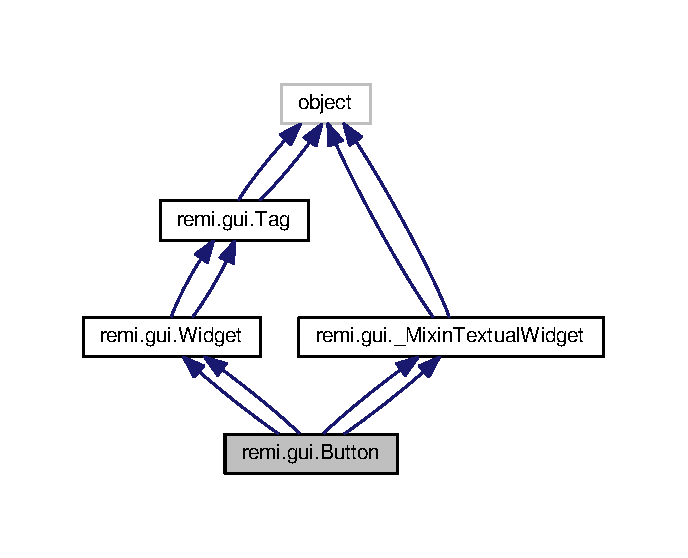
\includegraphics[width=330pt]{d5/d6e/classremi_1_1gui_1_1Button__inherit__graph}
\end{center}
\end{figure}


Collaboration diagram for remi.\+gui.\+Button\+:
\nopagebreak
\begin{figure}[H]
\begin{center}
\leavevmode
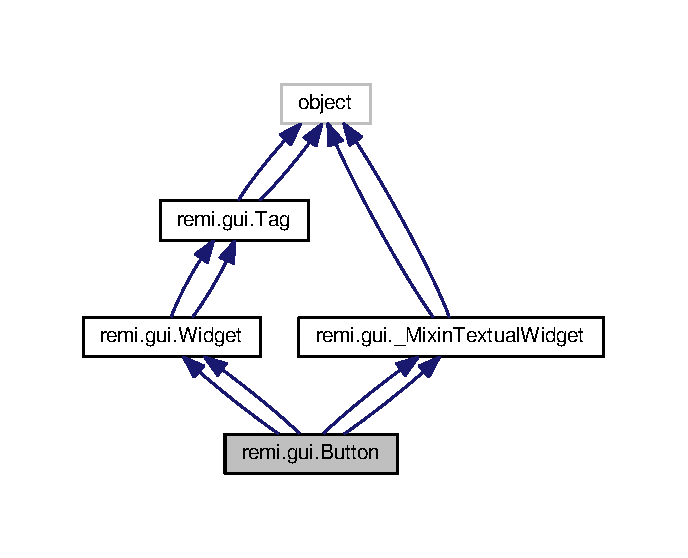
\includegraphics[width=330pt]{dd/db3/classremi_1_1gui_1_1Button__coll__graph}
\end{center}
\end{figure}
\subsection*{Public Member Functions}
\begin{DoxyCompactItemize}
\item 
def \hyperlink{classremi_1_1gui_1_1Button_a3384a4af97081503d5cbccc4ff3f3608}{\+\_\+\+\_\+init\+\_\+\+\_\+} (self, text=\textquotesingle{}\textquotesingle{}, kwargs)
\item 
def \hyperlink{classremi_1_1gui_1_1Button_a3384a4af97081503d5cbccc4ff3f3608}{\+\_\+\+\_\+init\+\_\+\+\_\+} (self, text=\textquotesingle{}\textquotesingle{}, kwargs)
\end{DoxyCompactItemize}
\subsection*{Public Attributes}
\begin{DoxyCompactItemize}
\item 
{\bfseries type}\hypertarget{classremi_1_1gui_1_1Button_a6d30954d2a6390dd3e5ecc6a87d3a5eb}{}\label{classremi_1_1gui_1_1Button_a6d30954d2a6390dd3e5ecc6a87d3a5eb}

\end{DoxyCompactItemize}
\subsection*{Additional Inherited Members}


\subsection{Detailed Description}
\begin{DoxyVerb}The Button widget. Have to be used in conjunction with its event onclick.
Use Widget.set_on_click_listener in order to register the listener.
\end{DoxyVerb}
 

\subsection{Constructor \& Destructor Documentation}
\index{remi\+::gui\+::\+Button@{remi\+::gui\+::\+Button}!\+\_\+\+\_\+init\+\_\+\+\_\+@{\+\_\+\+\_\+init\+\_\+\+\_\+}}
\index{\+\_\+\+\_\+init\+\_\+\+\_\+@{\+\_\+\+\_\+init\+\_\+\+\_\+}!remi\+::gui\+::\+Button@{remi\+::gui\+::\+Button}}
\subsubsection[{\texorpdfstring{\+\_\+\+\_\+init\+\_\+\+\_\+(self, text=\textquotesingle{}\textquotesingle{}, kwargs)}{__init__(self, text='', kwargs)}}]{\setlength{\rightskip}{0pt plus 5cm}def remi.\+gui.\+Button.\+\_\+\+\_\+init\+\_\+\+\_\+ (
\begin{DoxyParamCaption}
\item[{}]{self, }
\item[{}]{text = {\ttfamily \textquotesingle{}\textquotesingle{}}, }
\item[{}]{kwargs}
\end{DoxyParamCaption}
)}\hypertarget{classremi_1_1gui_1_1Button_a3384a4af97081503d5cbccc4ff3f3608}{}\label{classremi_1_1gui_1_1Button_a3384a4af97081503d5cbccc4ff3f3608}
\begin{DoxyVerb}Args:
    text (str): The text that will be displayed on the button.
    kwargs: See Widget.__init__()
\end{DoxyVerb}
 \index{remi\+::gui\+::\+Button@{remi\+::gui\+::\+Button}!\+\_\+\+\_\+init\+\_\+\+\_\+@{\+\_\+\+\_\+init\+\_\+\+\_\+}}
\index{\+\_\+\+\_\+init\+\_\+\+\_\+@{\+\_\+\+\_\+init\+\_\+\+\_\+}!remi\+::gui\+::\+Button@{remi\+::gui\+::\+Button}}
\subsubsection[{\texorpdfstring{\+\_\+\+\_\+init\+\_\+\+\_\+(self, text=\textquotesingle{}\textquotesingle{}, kwargs)}{__init__(self, text='', kwargs)}}]{\setlength{\rightskip}{0pt plus 5cm}def remi.\+gui.\+Button.\+\_\+\+\_\+init\+\_\+\+\_\+ (
\begin{DoxyParamCaption}
\item[{}]{self, }
\item[{}]{text = {\ttfamily \textquotesingle{}\textquotesingle{}}, }
\item[{}]{kwargs}
\end{DoxyParamCaption}
)}\hypertarget{classremi_1_1gui_1_1Button_a3384a4af97081503d5cbccc4ff3f3608}{}\label{classremi_1_1gui_1_1Button_a3384a4af97081503d5cbccc4ff3f3608}
\begin{DoxyVerb}Args:
    text (str): The text that will be displayed on the button.
    kwargs: See Widget.__init__()
\end{DoxyVerb}
 

The documentation for this class was generated from the following file\+:\begin{DoxyCompactItemize}
\item 
Compiled/\+Server/remi/gui.\+py\end{DoxyCompactItemize}

\hypertarget{classremi_1_1gui_1_1CheckBox}{}\section{remi.\+gui.\+Check\+Box Class Reference}
\label{classremi_1_1gui_1_1CheckBox}\index{remi.\+gui.\+Check\+Box@{remi.\+gui.\+Check\+Box}}


Inheritance diagram for remi.\+gui.\+Check\+Box\+:
\nopagebreak
\begin{figure}[H]
\begin{center}
\leavevmode
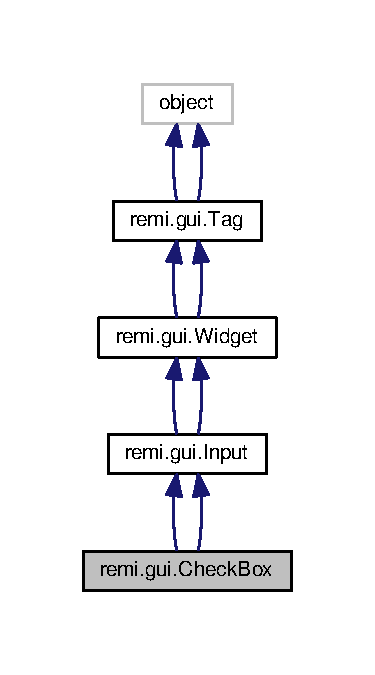
\includegraphics[width=180pt]{db/d2e/classremi_1_1gui_1_1CheckBox__inherit__graph}
\end{center}
\end{figure}


Collaboration diagram for remi.\+gui.\+Check\+Box\+:
\nopagebreak
\begin{figure}[H]
\begin{center}
\leavevmode
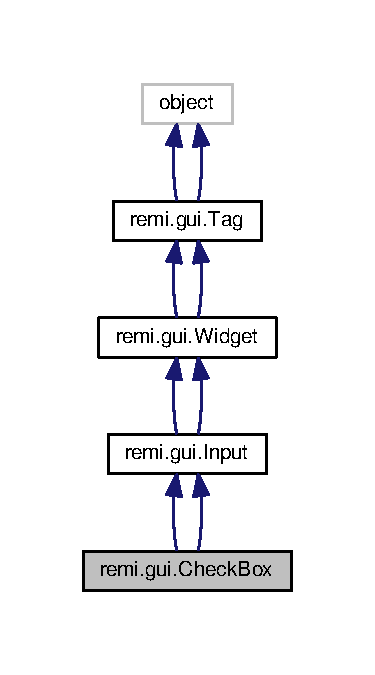
\includegraphics[width=180pt]{db/d6f/classremi_1_1gui_1_1CheckBox__coll__graph}
\end{center}
\end{figure}
\subsection*{Public Member Functions}
\begin{DoxyCompactItemize}
\item 
def \hyperlink{classremi_1_1gui_1_1CheckBox_a11912d6beb33eefc0ebc9f2c222b087f}{\+\_\+\+\_\+init\+\_\+\+\_\+} (self, checked=False, user\+\_\+data=\textquotesingle{}\textquotesingle{}, kwargs)
\item 
def \hyperlink{classremi_1_1gui_1_1CheckBox_aed8a3cd38f85743b5fc683c4797f4c97}{onchange} (self, value)
\item 
def \hyperlink{classremi_1_1gui_1_1CheckBox_a82f943b27590b9fb710095405b9107c8}{set\+\_\+value} (self, checked, update\+\_\+ui=1)
\item 
def \hyperlink{classremi_1_1gui_1_1CheckBox_a83ff74e6f93b02e36ee9262049064cbc}{get\+\_\+value} (self)
\item 
def \hyperlink{classremi_1_1gui_1_1CheckBox_a11912d6beb33eefc0ebc9f2c222b087f}{\+\_\+\+\_\+init\+\_\+\+\_\+} (self, checked=False, user\+\_\+data=\textquotesingle{}\textquotesingle{}, kwargs)
\item 
def \hyperlink{classremi_1_1gui_1_1CheckBox_aed8a3cd38f85743b5fc683c4797f4c97}{onchange} (self, value)
\item 
def \hyperlink{classremi_1_1gui_1_1CheckBox_a82f943b27590b9fb710095405b9107c8}{set\+\_\+value} (self, checked, update\+\_\+ui=1)
\item 
def \hyperlink{classremi_1_1gui_1_1CheckBox_a83ff74e6f93b02e36ee9262049064cbc}{get\+\_\+value} (self)
\end{DoxyCompactItemize}
\subsection*{Additional Inherited Members}


\subsection{Detailed Description}
\begin{DoxyVerb}check box widget useful as numeric input field implements the onchange event.\end{DoxyVerb}
 

\subsection{Constructor \& Destructor Documentation}
\index{remi\+::gui\+::\+Check\+Box@{remi\+::gui\+::\+Check\+Box}!\+\_\+\+\_\+init\+\_\+\+\_\+@{\+\_\+\+\_\+init\+\_\+\+\_\+}}
\index{\+\_\+\+\_\+init\+\_\+\+\_\+@{\+\_\+\+\_\+init\+\_\+\+\_\+}!remi\+::gui\+::\+Check\+Box@{remi\+::gui\+::\+Check\+Box}}
\subsubsection[{\texorpdfstring{\+\_\+\+\_\+init\+\_\+\+\_\+(self, checked=\+False, user\+\_\+data=\textquotesingle{}\textquotesingle{}, kwargs)}{__init__(self, checked=False, user_data='', kwargs)}}]{\setlength{\rightskip}{0pt plus 5cm}def remi.\+gui.\+Check\+Box.\+\_\+\+\_\+init\+\_\+\+\_\+ (
\begin{DoxyParamCaption}
\item[{}]{self, }
\item[{}]{checked = {\ttfamily False}, }
\item[{}]{user\+\_\+data = {\ttfamily \textquotesingle{}\textquotesingle{}}, }
\item[{}]{kwargs}
\end{DoxyParamCaption}
)}\hypertarget{classremi_1_1gui_1_1CheckBox_a11912d6beb33eefc0ebc9f2c222b087f}{}\label{classremi_1_1gui_1_1CheckBox_a11912d6beb33eefc0ebc9f2c222b087f}
\begin{DoxyVerb}Args:
    checked (bool):
    user_data (str):
    kwargs: See Widget.__init__()
\end{DoxyVerb}
 \index{remi\+::gui\+::\+Check\+Box@{remi\+::gui\+::\+Check\+Box}!\+\_\+\+\_\+init\+\_\+\+\_\+@{\+\_\+\+\_\+init\+\_\+\+\_\+}}
\index{\+\_\+\+\_\+init\+\_\+\+\_\+@{\+\_\+\+\_\+init\+\_\+\+\_\+}!remi\+::gui\+::\+Check\+Box@{remi\+::gui\+::\+Check\+Box}}
\subsubsection[{\texorpdfstring{\+\_\+\+\_\+init\+\_\+\+\_\+(self, checked=\+False, user\+\_\+data=\textquotesingle{}\textquotesingle{}, kwargs)}{__init__(self, checked=False, user_data='', kwargs)}}]{\setlength{\rightskip}{0pt plus 5cm}def remi.\+gui.\+Check\+Box.\+\_\+\+\_\+init\+\_\+\+\_\+ (
\begin{DoxyParamCaption}
\item[{}]{self, }
\item[{}]{checked = {\ttfamily False}, }
\item[{}]{user\+\_\+data = {\ttfamily \textquotesingle{}\textquotesingle{}}, }
\item[{}]{kwargs}
\end{DoxyParamCaption}
)}\hypertarget{classremi_1_1gui_1_1CheckBox_a11912d6beb33eefc0ebc9f2c222b087f}{}\label{classremi_1_1gui_1_1CheckBox_a11912d6beb33eefc0ebc9f2c222b087f}
\begin{DoxyVerb}Args:
    checked (bool):
    user_data (str):
    kwargs: See Widget.__init__()
\end{DoxyVerb}
 

\subsection{Member Function Documentation}
\index{remi\+::gui\+::\+Check\+Box@{remi\+::gui\+::\+Check\+Box}!get\+\_\+value@{get\+\_\+value}}
\index{get\+\_\+value@{get\+\_\+value}!remi\+::gui\+::\+Check\+Box@{remi\+::gui\+::\+Check\+Box}}
\subsubsection[{\texorpdfstring{get\+\_\+value(self)}{get_value(self)}}]{\setlength{\rightskip}{0pt plus 5cm}def remi.\+gui.\+Check\+Box.\+get\+\_\+value (
\begin{DoxyParamCaption}
\item[{}]{self}
\end{DoxyParamCaption}
)}\hypertarget{classremi_1_1gui_1_1CheckBox_a83ff74e6f93b02e36ee9262049064cbc}{}\label{classremi_1_1gui_1_1CheckBox_a83ff74e6f93b02e36ee9262049064cbc}
\begin{DoxyVerb}Returns:
    bool:
\end{DoxyVerb}
 \index{remi\+::gui\+::\+Check\+Box@{remi\+::gui\+::\+Check\+Box}!get\+\_\+value@{get\+\_\+value}}
\index{get\+\_\+value@{get\+\_\+value}!remi\+::gui\+::\+Check\+Box@{remi\+::gui\+::\+Check\+Box}}
\subsubsection[{\texorpdfstring{get\+\_\+value(self)}{get_value(self)}}]{\setlength{\rightskip}{0pt plus 5cm}def remi.\+gui.\+Check\+Box.\+get\+\_\+value (
\begin{DoxyParamCaption}
\item[{}]{self}
\end{DoxyParamCaption}
)}\hypertarget{classremi_1_1gui_1_1CheckBox_a83ff74e6f93b02e36ee9262049064cbc}{}\label{classremi_1_1gui_1_1CheckBox_a83ff74e6f93b02e36ee9262049064cbc}
\begin{DoxyVerb}Returns:
    bool:
\end{DoxyVerb}
 \index{remi\+::gui\+::\+Check\+Box@{remi\+::gui\+::\+Check\+Box}!onchange@{onchange}}
\index{onchange@{onchange}!remi\+::gui\+::\+Check\+Box@{remi\+::gui\+::\+Check\+Box}}
\subsubsection[{\texorpdfstring{onchange(self, value)}{onchange(self, value)}}]{\setlength{\rightskip}{0pt plus 5cm}def remi.\+gui.\+Check\+Box.\+onchange (
\begin{DoxyParamCaption}
\item[{}]{self, }
\item[{}]{value}
\end{DoxyParamCaption}
)}\hypertarget{classremi_1_1gui_1_1CheckBox_aed8a3cd38f85743b5fc683c4797f4c97}{}\label{classremi_1_1gui_1_1CheckBox_aed8a3cd38f85743b5fc683c4797f4c97}
\begin{DoxyVerb}Args:
    value:

Returns:\end{DoxyVerb}
 \index{remi\+::gui\+::\+Check\+Box@{remi\+::gui\+::\+Check\+Box}!onchange@{onchange}}
\index{onchange@{onchange}!remi\+::gui\+::\+Check\+Box@{remi\+::gui\+::\+Check\+Box}}
\subsubsection[{\texorpdfstring{onchange(self, value)}{onchange(self, value)}}]{\setlength{\rightskip}{0pt plus 5cm}def remi.\+gui.\+Check\+Box.\+onchange (
\begin{DoxyParamCaption}
\item[{}]{self, }
\item[{}]{value}
\end{DoxyParamCaption}
)}\hypertarget{classremi_1_1gui_1_1CheckBox_aed8a3cd38f85743b5fc683c4797f4c97}{}\label{classremi_1_1gui_1_1CheckBox_aed8a3cd38f85743b5fc683c4797f4c97}
\begin{DoxyVerb}Args:
    value:

Returns:\end{DoxyVerb}
 \index{remi\+::gui\+::\+Check\+Box@{remi\+::gui\+::\+Check\+Box}!set\+\_\+value@{set\+\_\+value}}
\index{set\+\_\+value@{set\+\_\+value}!remi\+::gui\+::\+Check\+Box@{remi\+::gui\+::\+Check\+Box}}
\subsubsection[{\texorpdfstring{set\+\_\+value(self, checked, update\+\_\+ui=1)}{set_value(self, checked, update_ui=1)}}]{\setlength{\rightskip}{0pt plus 5cm}def remi.\+gui.\+Check\+Box.\+set\+\_\+value (
\begin{DoxyParamCaption}
\item[{}]{self, }
\item[{}]{checked, }
\item[{}]{update\+\_\+ui = {\ttfamily 1}}
\end{DoxyParamCaption}
)}\hypertarget{classremi_1_1gui_1_1CheckBox_a82f943b27590b9fb710095405b9107c8}{}\label{classremi_1_1gui_1_1CheckBox_a82f943b27590b9fb710095405b9107c8}
\begin{DoxyVerb}Args:
    checked:
    update_ui:
\end{DoxyVerb}
 \index{remi\+::gui\+::\+Check\+Box@{remi\+::gui\+::\+Check\+Box}!set\+\_\+value@{set\+\_\+value}}
\index{set\+\_\+value@{set\+\_\+value}!remi\+::gui\+::\+Check\+Box@{remi\+::gui\+::\+Check\+Box}}
\subsubsection[{\texorpdfstring{set\+\_\+value(self, checked, update\+\_\+ui=1)}{set_value(self, checked, update_ui=1)}}]{\setlength{\rightskip}{0pt plus 5cm}def remi.\+gui.\+Check\+Box.\+set\+\_\+value (
\begin{DoxyParamCaption}
\item[{}]{self, }
\item[{}]{checked, }
\item[{}]{update\+\_\+ui = {\ttfamily 1}}
\end{DoxyParamCaption}
)}\hypertarget{classremi_1_1gui_1_1CheckBox_a82f943b27590b9fb710095405b9107c8}{}\label{classremi_1_1gui_1_1CheckBox_a82f943b27590b9fb710095405b9107c8}
\begin{DoxyVerb}Args:
    checked:
    update_ui:
\end{DoxyVerb}
 

The documentation for this class was generated from the following file\+:\begin{DoxyCompactItemize}
\item 
Compiled/\+Server/remi/gui.\+py\end{DoxyCompactItemize}

\hypertarget{classremi_1_1gui_1_1CheckBoxLabel}{}\section{remi.\+gui.\+Check\+Box\+Label Class Reference}
\label{classremi_1_1gui_1_1CheckBoxLabel}\index{remi.\+gui.\+Check\+Box\+Label@{remi.\+gui.\+Check\+Box\+Label}}


Inheritance diagram for remi.\+gui.\+Check\+Box\+Label\+:
\nopagebreak
\begin{figure}[H]
\begin{center}
\leavevmode
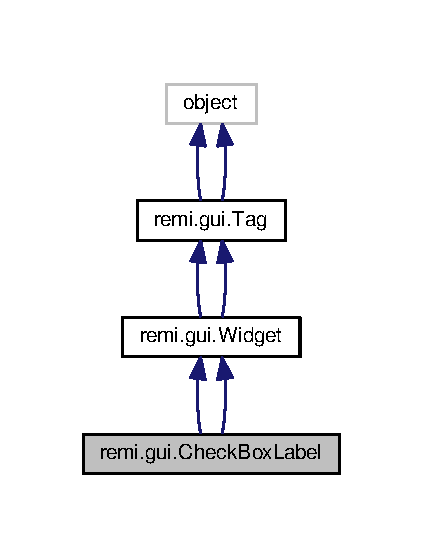
\includegraphics[width=203pt]{d4/d3c/classremi_1_1gui_1_1CheckBoxLabel__inherit__graph}
\end{center}
\end{figure}


Collaboration diagram for remi.\+gui.\+Check\+Box\+Label\+:
\nopagebreak
\begin{figure}[H]
\begin{center}
\leavevmode
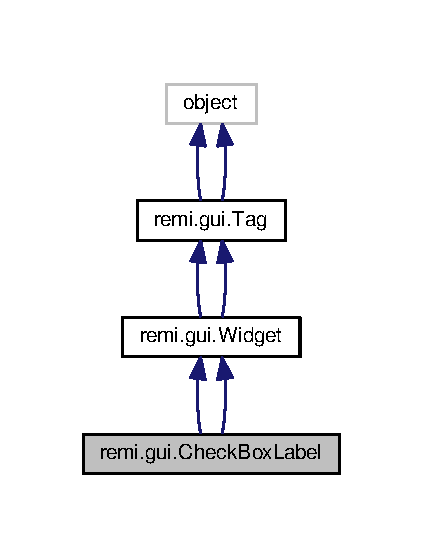
\includegraphics[width=203pt]{dc/dba/classremi_1_1gui_1_1CheckBoxLabel__coll__graph}
\end{center}
\end{figure}
\subsection*{Public Member Functions}
\begin{DoxyCompactItemize}
\item 
def \hyperlink{classremi_1_1gui_1_1CheckBoxLabel_a65c074b3fdc5a54c906038a6f788aa71}{\+\_\+\+\_\+init\+\_\+\+\_\+} (self, label=\textquotesingle{}\textquotesingle{}, checked=False, user\+\_\+data=\textquotesingle{}\textquotesingle{}, kwargs)
\item 
def \hyperlink{classremi_1_1gui_1_1CheckBoxLabel_af0bf9ccc18775950a3362c4f96250d2d}{onchange} (self, widget, value)
\item 
def \hyperlink{classremi_1_1gui_1_1CheckBoxLabel_a51cc055995154f93ed4483de62d709f7}{set\+\_\+on\+\_\+change\+\_\+listener} (self, callback, userdata)
\item 
def \hyperlink{classremi_1_1gui_1_1CheckBoxLabel_a65c074b3fdc5a54c906038a6f788aa71}{\+\_\+\+\_\+init\+\_\+\+\_\+} (self, label=\textquotesingle{}\textquotesingle{}, checked=False, user\+\_\+data=\textquotesingle{}\textquotesingle{}, kwargs)
\item 
def \hyperlink{classremi_1_1gui_1_1CheckBoxLabel_af0bf9ccc18775950a3362c4f96250d2d}{onchange} (self, widget, value)
\item 
def \hyperlink{classremi_1_1gui_1_1CheckBoxLabel_a51cc055995154f93ed4483de62d709f7}{set\+\_\+on\+\_\+change\+\_\+listener} (self, callback, userdata)
\end{DoxyCompactItemize}
\subsection*{Public Attributes}
\begin{DoxyCompactItemize}
\item 
{\bfseries set\+\_\+value}\hypertarget{classremi_1_1gui_1_1CheckBoxLabel_a345caf89b8a86e8d5daa9eac3f995fbc}{}\label{classremi_1_1gui_1_1CheckBoxLabel_a345caf89b8a86e8d5daa9eac3f995fbc}

\item 
{\bfseries get\+\_\+value}\hypertarget{classremi_1_1gui_1_1CheckBoxLabel_a903f712e42a58feb5a019b4e52cec75c}{}\label{classremi_1_1gui_1_1CheckBoxLabel_a903f712e42a58feb5a019b4e52cec75c}

\end{DoxyCompactItemize}
\subsection*{Additional Inherited Members}


\subsection{Detailed Description}
\begin{DoxyVerb}\end{DoxyVerb}
 

\subsection{Constructor \& Destructor Documentation}
\index{remi\+::gui\+::\+Check\+Box\+Label@{remi\+::gui\+::\+Check\+Box\+Label}!\+\_\+\+\_\+init\+\_\+\+\_\+@{\+\_\+\+\_\+init\+\_\+\+\_\+}}
\index{\+\_\+\+\_\+init\+\_\+\+\_\+@{\+\_\+\+\_\+init\+\_\+\+\_\+}!remi\+::gui\+::\+Check\+Box\+Label@{remi\+::gui\+::\+Check\+Box\+Label}}
\subsubsection[{\texorpdfstring{\+\_\+\+\_\+init\+\_\+\+\_\+(self, label=\textquotesingle{}\textquotesingle{}, checked=\+False, user\+\_\+data=\textquotesingle{}\textquotesingle{}, kwargs)}{__init__(self, label='', checked=False, user_data='', kwargs)}}]{\setlength{\rightskip}{0pt plus 5cm}def remi.\+gui.\+Check\+Box\+Label.\+\_\+\+\_\+init\+\_\+\+\_\+ (
\begin{DoxyParamCaption}
\item[{}]{self, }
\item[{}]{label = {\ttfamily \textquotesingle{}\textquotesingle{}}, }
\item[{}]{checked = {\ttfamily False}, }
\item[{}]{user\+\_\+data = {\ttfamily \textquotesingle{}\textquotesingle{}}, }
\item[{}]{kwargs}
\end{DoxyParamCaption}
)}\hypertarget{classremi_1_1gui_1_1CheckBoxLabel_a65c074b3fdc5a54c906038a6f788aa71}{}\label{classremi_1_1gui_1_1CheckBoxLabel_a65c074b3fdc5a54c906038a6f788aa71}
\begin{DoxyVerb}Args:
    label (str):
    checked (bool):
    user_data (str):
    kwargs: See Widget.__init__()
\end{DoxyVerb}
 \index{remi\+::gui\+::\+Check\+Box\+Label@{remi\+::gui\+::\+Check\+Box\+Label}!\+\_\+\+\_\+init\+\_\+\+\_\+@{\+\_\+\+\_\+init\+\_\+\+\_\+}}
\index{\+\_\+\+\_\+init\+\_\+\+\_\+@{\+\_\+\+\_\+init\+\_\+\+\_\+}!remi\+::gui\+::\+Check\+Box\+Label@{remi\+::gui\+::\+Check\+Box\+Label}}
\subsubsection[{\texorpdfstring{\+\_\+\+\_\+init\+\_\+\+\_\+(self, label=\textquotesingle{}\textquotesingle{}, checked=\+False, user\+\_\+data=\textquotesingle{}\textquotesingle{}, kwargs)}{__init__(self, label='', checked=False, user_data='', kwargs)}}]{\setlength{\rightskip}{0pt plus 5cm}def remi.\+gui.\+Check\+Box\+Label.\+\_\+\+\_\+init\+\_\+\+\_\+ (
\begin{DoxyParamCaption}
\item[{}]{self, }
\item[{}]{label = {\ttfamily \textquotesingle{}\textquotesingle{}}, }
\item[{}]{checked = {\ttfamily False}, }
\item[{}]{user\+\_\+data = {\ttfamily \textquotesingle{}\textquotesingle{}}, }
\item[{}]{kwargs}
\end{DoxyParamCaption}
)}\hypertarget{classremi_1_1gui_1_1CheckBoxLabel_a65c074b3fdc5a54c906038a6f788aa71}{}\label{classremi_1_1gui_1_1CheckBoxLabel_a65c074b3fdc5a54c906038a6f788aa71}
\begin{DoxyVerb}Args:
    label (str):
    checked (bool):
    user_data (str):
    kwargs: See Widget.__init__()
\end{DoxyVerb}
 

\subsection{Member Function Documentation}
\index{remi\+::gui\+::\+Check\+Box\+Label@{remi\+::gui\+::\+Check\+Box\+Label}!onchange@{onchange}}
\index{onchange@{onchange}!remi\+::gui\+::\+Check\+Box\+Label@{remi\+::gui\+::\+Check\+Box\+Label}}
\subsubsection[{\texorpdfstring{onchange(self, widget, value)}{onchange(self, widget, value)}}]{\setlength{\rightskip}{0pt plus 5cm}def remi.\+gui.\+Check\+Box\+Label.\+onchange (
\begin{DoxyParamCaption}
\item[{}]{self, }
\item[{}]{widget, }
\item[{}]{value}
\end{DoxyParamCaption}
)}\hypertarget{classremi_1_1gui_1_1CheckBoxLabel_af0bf9ccc18775950a3362c4f96250d2d}{}\label{classremi_1_1gui_1_1CheckBoxLabel_af0bf9ccc18775950a3362c4f96250d2d}
\begin{DoxyVerb}Args:
    widget:
    value:

Returns:\end{DoxyVerb}
 \index{remi\+::gui\+::\+Check\+Box\+Label@{remi\+::gui\+::\+Check\+Box\+Label}!onchange@{onchange}}
\index{onchange@{onchange}!remi\+::gui\+::\+Check\+Box\+Label@{remi\+::gui\+::\+Check\+Box\+Label}}
\subsubsection[{\texorpdfstring{onchange(self, widget, value)}{onchange(self, widget, value)}}]{\setlength{\rightskip}{0pt plus 5cm}def remi.\+gui.\+Check\+Box\+Label.\+onchange (
\begin{DoxyParamCaption}
\item[{}]{self, }
\item[{}]{widget, }
\item[{}]{value}
\end{DoxyParamCaption}
)}\hypertarget{classremi_1_1gui_1_1CheckBoxLabel_af0bf9ccc18775950a3362c4f96250d2d}{}\label{classremi_1_1gui_1_1CheckBoxLabel_af0bf9ccc18775950a3362c4f96250d2d}
\begin{DoxyVerb}Args:
    widget:
    value:

Returns:\end{DoxyVerb}
 \index{remi\+::gui\+::\+Check\+Box\+Label@{remi\+::gui\+::\+Check\+Box\+Label}!set\+\_\+on\+\_\+change\+\_\+listener@{set\+\_\+on\+\_\+change\+\_\+listener}}
\index{set\+\_\+on\+\_\+change\+\_\+listener@{set\+\_\+on\+\_\+change\+\_\+listener}!remi\+::gui\+::\+Check\+Box\+Label@{remi\+::gui\+::\+Check\+Box\+Label}}
\subsubsection[{\texorpdfstring{set\+\_\+on\+\_\+change\+\_\+listener(self, callback, userdata)}{set_on_change_listener(self, callback, userdata)}}]{\setlength{\rightskip}{0pt plus 5cm}def remi.\+gui.\+Check\+Box\+Label.\+set\+\_\+on\+\_\+change\+\_\+listener (
\begin{DoxyParamCaption}
\item[{}]{self, }
\item[{}]{callback, }
\item[{}]{userdata}
\end{DoxyParamCaption}
)}\hypertarget{classremi_1_1gui_1_1CheckBoxLabel_a51cc055995154f93ed4483de62d709f7}{}\label{classremi_1_1gui_1_1CheckBoxLabel_a51cc055995154f93ed4483de62d709f7}
\begin{DoxyVerb}Args:
    callback:
    userdata:
\end{DoxyVerb}
 \index{remi\+::gui\+::\+Check\+Box\+Label@{remi\+::gui\+::\+Check\+Box\+Label}!set\+\_\+on\+\_\+change\+\_\+listener@{set\+\_\+on\+\_\+change\+\_\+listener}}
\index{set\+\_\+on\+\_\+change\+\_\+listener@{set\+\_\+on\+\_\+change\+\_\+listener}!remi\+::gui\+::\+Check\+Box\+Label@{remi\+::gui\+::\+Check\+Box\+Label}}
\subsubsection[{\texorpdfstring{set\+\_\+on\+\_\+change\+\_\+listener(self, callback, userdata)}{set_on_change_listener(self, callback, userdata)}}]{\setlength{\rightskip}{0pt plus 5cm}def remi.\+gui.\+Check\+Box\+Label.\+set\+\_\+on\+\_\+change\+\_\+listener (
\begin{DoxyParamCaption}
\item[{}]{self, }
\item[{}]{callback, }
\item[{}]{userdata}
\end{DoxyParamCaption}
)}\hypertarget{classremi_1_1gui_1_1CheckBoxLabel_a51cc055995154f93ed4483de62d709f7}{}\label{classremi_1_1gui_1_1CheckBoxLabel_a51cc055995154f93ed4483de62d709f7}
\begin{DoxyVerb}Args:
    callback:
    userdata:
\end{DoxyVerb}
 

The documentation for this class was generated from the following file\+:\begin{DoxyCompactItemize}
\item 
Compiled/\+Server/remi/gui.\+py\end{DoxyCompactItemize}

\hypertarget{classremi_1_1gui_1_1ColorPicker}{}\section{remi.\+gui.\+Color\+Picker Class Reference}
\label{classremi_1_1gui_1_1ColorPicker}\index{remi.\+gui.\+Color\+Picker@{remi.\+gui.\+Color\+Picker}}


Inheritance diagram for remi.\+gui.\+Color\+Picker\+:
\nopagebreak
\begin{figure}[H]
\begin{center}
\leavevmode
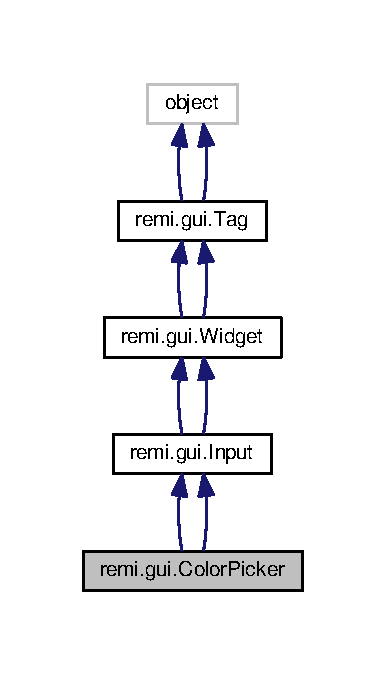
\includegraphics[width=185pt]{d1/d7d/classremi_1_1gui_1_1ColorPicker__inherit__graph}
\end{center}
\end{figure}


Collaboration diagram for remi.\+gui.\+Color\+Picker\+:
\nopagebreak
\begin{figure}[H]
\begin{center}
\leavevmode
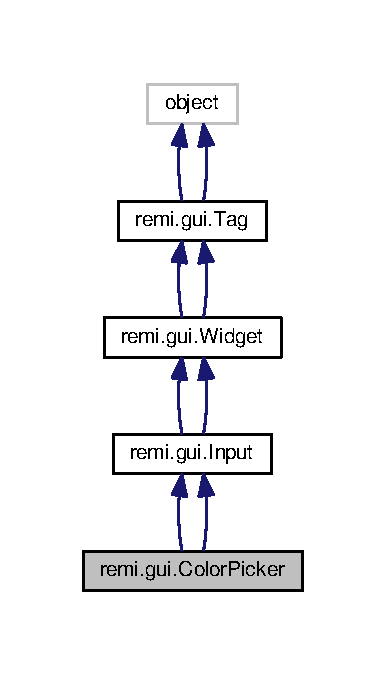
\includegraphics[width=185pt]{d6/df9/classremi_1_1gui_1_1ColorPicker__coll__graph}
\end{center}
\end{figure}
\subsection*{Public Member Functions}
\begin{DoxyCompactItemize}
\item 
def \hyperlink{classremi_1_1gui_1_1ColorPicker_a5b0559ebc85e0ea86d569cdc5bd475e7}{\+\_\+\+\_\+init\+\_\+\+\_\+} (self, default\+\_\+value=\textquotesingle{}\#995500\textquotesingle{}, kwargs)
\item 
def \hyperlink{classremi_1_1gui_1_1ColorPicker_a5b0559ebc85e0ea86d569cdc5bd475e7}{\+\_\+\+\_\+init\+\_\+\+\_\+} (self, default\+\_\+value=\textquotesingle{}\#995500\textquotesingle{}, kwargs)
\end{DoxyCompactItemize}
\subsection*{Additional Inherited Members}


\subsection{Detailed Description}
\begin{DoxyVerb}\end{DoxyVerb}
 

\subsection{Constructor \& Destructor Documentation}
\index{remi\+::gui\+::\+Color\+Picker@{remi\+::gui\+::\+Color\+Picker}!\+\_\+\+\_\+init\+\_\+\+\_\+@{\+\_\+\+\_\+init\+\_\+\+\_\+}}
\index{\+\_\+\+\_\+init\+\_\+\+\_\+@{\+\_\+\+\_\+init\+\_\+\+\_\+}!remi\+::gui\+::\+Color\+Picker@{remi\+::gui\+::\+Color\+Picker}}
\subsubsection[{\texorpdfstring{\+\_\+\+\_\+init\+\_\+\+\_\+(self, default\+\_\+value=\textquotesingle{}\#995500\textquotesingle{}, kwargs)}{__init__(self, default_value='#995500', kwargs)}}]{\setlength{\rightskip}{0pt plus 5cm}def remi.\+gui.\+Color\+Picker.\+\_\+\+\_\+init\+\_\+\+\_\+ (
\begin{DoxyParamCaption}
\item[{}]{self, }
\item[{}]{default\+\_\+value = {\ttfamily \textquotesingle{}\#995500\textquotesingle{}}, }
\item[{}]{kwargs}
\end{DoxyParamCaption}
)}\hypertarget{classremi_1_1gui_1_1ColorPicker_a5b0559ebc85e0ea86d569cdc5bd475e7}{}\label{classremi_1_1gui_1_1ColorPicker_a5b0559ebc85e0ea86d569cdc5bd475e7}
\begin{DoxyVerb}Args:
    default_value (str): hex rgb color string (#rrggbb)
    kwargs: See Widget.__init__()
\end{DoxyVerb}
 \index{remi\+::gui\+::\+Color\+Picker@{remi\+::gui\+::\+Color\+Picker}!\+\_\+\+\_\+init\+\_\+\+\_\+@{\+\_\+\+\_\+init\+\_\+\+\_\+}}
\index{\+\_\+\+\_\+init\+\_\+\+\_\+@{\+\_\+\+\_\+init\+\_\+\+\_\+}!remi\+::gui\+::\+Color\+Picker@{remi\+::gui\+::\+Color\+Picker}}
\subsubsection[{\texorpdfstring{\+\_\+\+\_\+init\+\_\+\+\_\+(self, default\+\_\+value=\textquotesingle{}\#995500\textquotesingle{}, kwargs)}{__init__(self, default_value='#995500', kwargs)}}]{\setlength{\rightskip}{0pt plus 5cm}def remi.\+gui.\+Color\+Picker.\+\_\+\+\_\+init\+\_\+\+\_\+ (
\begin{DoxyParamCaption}
\item[{}]{self, }
\item[{}]{default\+\_\+value = {\ttfamily \textquotesingle{}\#995500\textquotesingle{}}, }
\item[{}]{kwargs}
\end{DoxyParamCaption}
)}\hypertarget{classremi_1_1gui_1_1ColorPicker_a5b0559ebc85e0ea86d569cdc5bd475e7}{}\label{classremi_1_1gui_1_1ColorPicker_a5b0559ebc85e0ea86d569cdc5bd475e7}
\begin{DoxyVerb}Args:
    default_value (str): hex rgb color string (#rrggbb)
    kwargs: See Widget.__init__()
\end{DoxyVerb}
 

The documentation for this class was generated from the following file\+:\begin{DoxyCompactItemize}
\item 
Compiled/\+Server/remi/gui.\+py\end{DoxyCompactItemize}

\hypertarget{structconnection__t}{}\section{Riferimenti per la struct connection\+\_\+t}
\label{structconnection__t}\index{connection\+\_\+t@{connection\+\_\+t}}
\subsection*{Campi}
\begin{DoxyCompactItemize}
\item 
int {\bfseries socket}\hypertarget{structconnection__t_a8739936cfe1c4e9f23368e375c976c92}{}\label{structconnection__t_a8739936cfe1c4e9f23368e375c976c92}

\item 
struct sockaddr\+\_\+in {\bfseries client\+Data}\hypertarget{structconnection__t_a2b4d38d53b1ca15e78ff677f8e6fc761}{}\label{structconnection__t_a2b4d38d53b1ca15e78ff677f8e6fc761}

\item 
socklen\+\_\+t {\bfseries client\+Data\+Lenght}\hypertarget{structconnection__t_ada2a0ae1a1bcf2709cfda2d95e9ac1a1}{}\label{structconnection__t_ada2a0ae1a1bcf2709cfda2d95e9ac1a1}

\end{DoxyCompactItemize}


La documentazione per questa struct è stata generata a partire dal seguente file\+:\begin{DoxyCompactItemize}
\item 
Networking/Networking.\+h\end{DoxyCompactItemize}

\hypertarget{classremi_1_1gui_1_1Date}{}\section{remi.\+gui.\+Date Class Reference}
\label{classremi_1_1gui_1_1Date}\index{remi.\+gui.\+Date@{remi.\+gui.\+Date}}


Inheritance diagram for remi.\+gui.\+Date\+:
\nopagebreak
\begin{figure}[H]
\begin{center}
\leavevmode
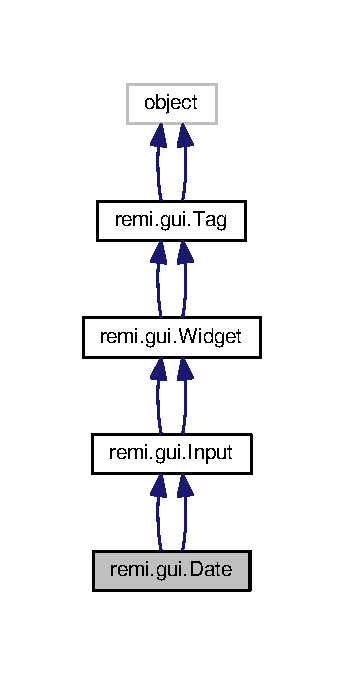
\includegraphics[width=165pt]{da/d08/classremi_1_1gui_1_1Date__inherit__graph}
\end{center}
\end{figure}


Collaboration diagram for remi.\+gui.\+Date\+:
\nopagebreak
\begin{figure}[H]
\begin{center}
\leavevmode
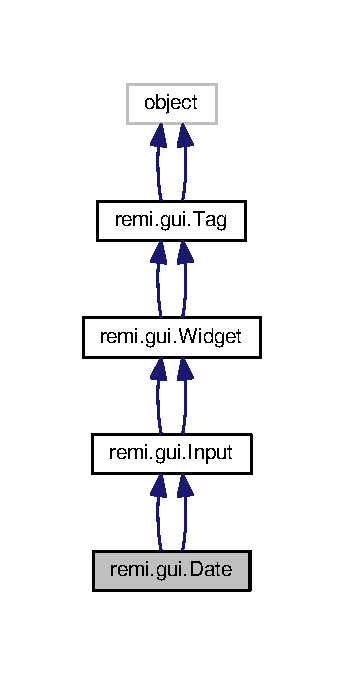
\includegraphics[width=165pt]{df/de4/classremi_1_1gui_1_1Date__coll__graph}
\end{center}
\end{figure}
\subsection*{Public Member Functions}
\begin{DoxyCompactItemize}
\item 
def \hyperlink{classremi_1_1gui_1_1Date_a72a0690165f29ee3ced491b1d2cac414}{\+\_\+\+\_\+init\+\_\+\+\_\+} (self, default\+\_\+value=\textquotesingle{}2015-\/04-\/13\textquotesingle{}, kwargs)
\item 
def \hyperlink{classremi_1_1gui_1_1Date_a72a0690165f29ee3ced491b1d2cac414}{\+\_\+\+\_\+init\+\_\+\+\_\+} (self, default\+\_\+value=\textquotesingle{}2015-\/04-\/13\textquotesingle{}, kwargs)
\end{DoxyCompactItemize}
\subsection*{Additional Inherited Members}


\subsection{Detailed Description}
\begin{DoxyVerb}\end{DoxyVerb}
 

\subsection{Constructor \& Destructor Documentation}
\index{remi\+::gui\+::\+Date@{remi\+::gui\+::\+Date}!\+\_\+\+\_\+init\+\_\+\+\_\+@{\+\_\+\+\_\+init\+\_\+\+\_\+}}
\index{\+\_\+\+\_\+init\+\_\+\+\_\+@{\+\_\+\+\_\+init\+\_\+\+\_\+}!remi\+::gui\+::\+Date@{remi\+::gui\+::\+Date}}
\subsubsection[{\texorpdfstring{\+\_\+\+\_\+init\+\_\+\+\_\+(self, default\+\_\+value=\textquotesingle{}2015-\/04-\/13\textquotesingle{}, kwargs)}{__init__(self, default_value='2015-04-13', kwargs)}}]{\setlength{\rightskip}{0pt plus 5cm}def remi.\+gui.\+Date.\+\_\+\+\_\+init\+\_\+\+\_\+ (
\begin{DoxyParamCaption}
\item[{}]{self, }
\item[{}]{default\+\_\+value = {\ttfamily \textquotesingle{}2015-\/04-\/13\textquotesingle{}}, }
\item[{}]{kwargs}
\end{DoxyParamCaption}
)}\hypertarget{classremi_1_1gui_1_1Date_a72a0690165f29ee3ced491b1d2cac414}{}\label{classremi_1_1gui_1_1Date_a72a0690165f29ee3ced491b1d2cac414}
\begin{DoxyVerb}Args:
    default_value (str): date string (yyyy-mm-dd)
    kwargs: See Widget.__init__()
\end{DoxyVerb}
 \index{remi\+::gui\+::\+Date@{remi\+::gui\+::\+Date}!\+\_\+\+\_\+init\+\_\+\+\_\+@{\+\_\+\+\_\+init\+\_\+\+\_\+}}
\index{\+\_\+\+\_\+init\+\_\+\+\_\+@{\+\_\+\+\_\+init\+\_\+\+\_\+}!remi\+::gui\+::\+Date@{remi\+::gui\+::\+Date}}
\subsubsection[{\texorpdfstring{\+\_\+\+\_\+init\+\_\+\+\_\+(self, default\+\_\+value=\textquotesingle{}2015-\/04-\/13\textquotesingle{}, kwargs)}{__init__(self, default_value='2015-04-13', kwargs)}}]{\setlength{\rightskip}{0pt plus 5cm}def remi.\+gui.\+Date.\+\_\+\+\_\+init\+\_\+\+\_\+ (
\begin{DoxyParamCaption}
\item[{}]{self, }
\item[{}]{default\+\_\+value = {\ttfamily \textquotesingle{}2015-\/04-\/13\textquotesingle{}}, }
\item[{}]{kwargs}
\end{DoxyParamCaption}
)}\hypertarget{classremi_1_1gui_1_1Date_a72a0690165f29ee3ced491b1d2cac414}{}\label{classremi_1_1gui_1_1Date_a72a0690165f29ee3ced491b1d2cac414}
\begin{DoxyVerb}Args:
    default_value (str): date string (yyyy-mm-dd)
    kwargs: See Widget.__init__()
\end{DoxyVerb}
 

The documentation for this class was generated from the following file\+:\begin{DoxyCompactItemize}
\item 
Compiled/\+Server/remi/gui.\+py\end{DoxyCompactItemize}

\hypertarget{classremi_1_1gui_1_1DropDown}{}\section{remi.\+gui.\+Drop\+Down Class Reference}
\label{classremi_1_1gui_1_1DropDown}\index{remi.\+gui.\+Drop\+Down@{remi.\+gui.\+Drop\+Down}}


Inheritance diagram for remi.\+gui.\+Drop\+Down\+:
\nopagebreak
\begin{figure}[H]
\begin{center}
\leavevmode
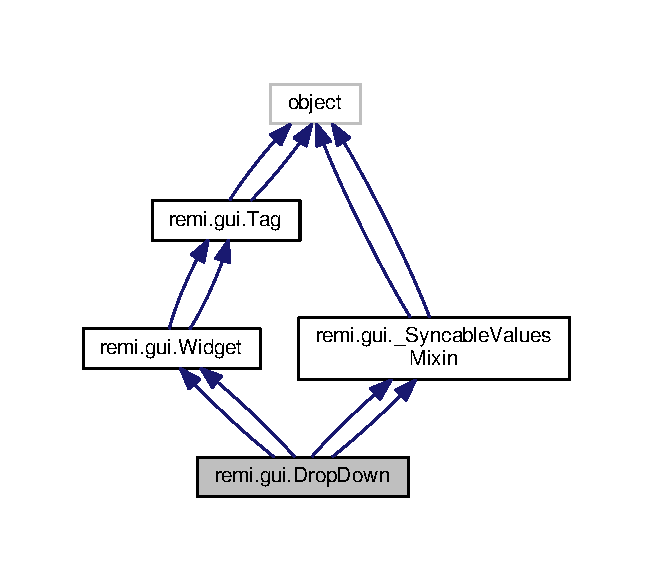
\includegraphics[width=314pt]{d1/dbd/classremi_1_1gui_1_1DropDown__inherit__graph}
\end{center}
\end{figure}


Collaboration diagram for remi.\+gui.\+Drop\+Down\+:
\nopagebreak
\begin{figure}[H]
\begin{center}
\leavevmode
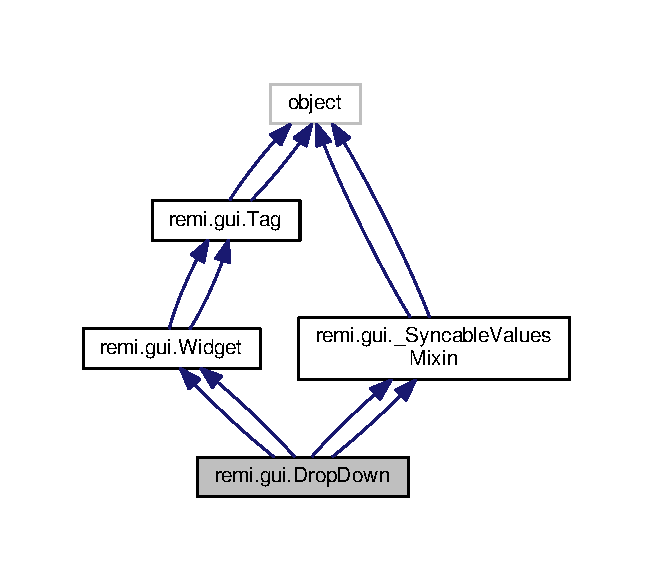
\includegraphics[width=314pt]{d2/d3d/classremi_1_1gui_1_1DropDown__coll__graph}
\end{center}
\end{figure}
\subsection*{Public Member Functions}
\begin{DoxyCompactItemize}
\item 
def \hyperlink{classremi_1_1gui_1_1DropDown_a4d64cb3276727de8098e9932869db09c}{\+\_\+\+\_\+init\+\_\+\+\_\+} (self, kwargs)
\item 
def \hyperlink{classremi_1_1gui_1_1DropDown_adb3c979c795d849686e3a33680697768}{new\+\_\+from\+\_\+list} (cls, items, kwargs)
\item 
def \hyperlink{classremi_1_1gui_1_1DropDown_a11d351d78669cfac0e8584f1c434fadc}{append} (self, item, key=\textquotesingle{}\textquotesingle{})
\item 
def \hyperlink{classremi_1_1gui_1_1DropDown_a0d08df5632bb86d7e080a0a16dfed81b}{empty} (self)
\item 
def \hyperlink{classremi_1_1gui_1_1DropDown_ab90bddfa11c58ca1f3dc511e71c208a0}{select\+\_\+by\+\_\+key} (self, key)
\item 
def \hyperlink{classremi_1_1gui_1_1DropDown_a4ae2ce02966ee50469ac41ebdabf69d8}{set\+\_\+value} (self, value)
\item 
def \hyperlink{classremi_1_1gui_1_1DropDown_a0ace4729ed7dcbeb794dd74c4319966b}{select\+\_\+by\+\_\+value} (self, value)
\item 
def \hyperlink{classremi_1_1gui_1_1DropDown_a27a3a7621118ca5a52aeaacc1727863d}{get\+\_\+value} (self)
\item 
def \hyperlink{classremi_1_1gui_1_1DropDown_ac68a8e0482c7bf82e57ca9cfc943be01}{get\+\_\+key} (self)
\item 
def \hyperlink{classremi_1_1gui_1_1DropDown_afc8c3b60e36d41160ca6fe5fb56188c4}{onchange} (self, value)
\item 
def \hyperlink{classremi_1_1gui_1_1DropDown_ae89e13b02debba198e4c8d30852e42e6}{set\+\_\+on\+\_\+change\+\_\+listener} (self, callback, userdata)
\item 
def \hyperlink{classremi_1_1gui_1_1DropDown_a4d64cb3276727de8098e9932869db09c}{\+\_\+\+\_\+init\+\_\+\+\_\+} (self, kwargs)
\item 
def \hyperlink{classremi_1_1gui_1_1DropDown_adb3c979c795d849686e3a33680697768}{new\+\_\+from\+\_\+list} (cls, items, kwargs)
\item 
def \hyperlink{classremi_1_1gui_1_1DropDown_a11d351d78669cfac0e8584f1c434fadc}{append} (self, item, key=\textquotesingle{}\textquotesingle{})
\item 
def \hyperlink{classremi_1_1gui_1_1DropDown_a0d08df5632bb86d7e080a0a16dfed81b}{empty} (self)
\item 
def \hyperlink{classremi_1_1gui_1_1DropDown_ab90bddfa11c58ca1f3dc511e71c208a0}{select\+\_\+by\+\_\+key} (self, key)
\item 
def \hyperlink{classremi_1_1gui_1_1DropDown_a4ae2ce02966ee50469ac41ebdabf69d8}{set\+\_\+value} (self, value)
\item 
def \hyperlink{classremi_1_1gui_1_1DropDown_a0ace4729ed7dcbeb794dd74c4319966b}{select\+\_\+by\+\_\+value} (self, value)
\item 
def \hyperlink{classremi_1_1gui_1_1DropDown_a27a3a7621118ca5a52aeaacc1727863d}{get\+\_\+value} (self)
\item 
def \hyperlink{classremi_1_1gui_1_1DropDown_ac68a8e0482c7bf82e57ca9cfc943be01}{get\+\_\+key} (self)
\item 
def \hyperlink{classremi_1_1gui_1_1DropDown_afc8c3b60e36d41160ca6fe5fb56188c4}{onchange} (self, value)
\item 
def \hyperlink{classremi_1_1gui_1_1DropDown_ae89e13b02debba198e4c8d30852e42e6}{set\+\_\+on\+\_\+change\+\_\+listener} (self, callback, userdata)
\end{DoxyCompactItemize}
\subsection*{Public Attributes}
\begin{DoxyCompactItemize}
\item 
{\bfseries type}\hypertarget{classremi_1_1gui_1_1DropDown_a71e6df9091a9b4c748f6d9771d23d858}{}\label{classremi_1_1gui_1_1DropDown_a71e6df9091a9b4c748f6d9771d23d858}

\end{DoxyCompactItemize}
\subsection*{Additional Inherited Members}


\subsection{Detailed Description}
\begin{DoxyVerb}Drop down selection widget. Implements the onchange(value) event. Register a listener for its selection change
by means of the function DropDown.set_on_change_listener.
\end{DoxyVerb}
 

\subsection{Constructor \& Destructor Documentation}
\index{remi\+::gui\+::\+Drop\+Down@{remi\+::gui\+::\+Drop\+Down}!\+\_\+\+\_\+init\+\_\+\+\_\+@{\+\_\+\+\_\+init\+\_\+\+\_\+}}
\index{\+\_\+\+\_\+init\+\_\+\+\_\+@{\+\_\+\+\_\+init\+\_\+\+\_\+}!remi\+::gui\+::\+Drop\+Down@{remi\+::gui\+::\+Drop\+Down}}
\subsubsection[{\texorpdfstring{\+\_\+\+\_\+init\+\_\+\+\_\+(self, kwargs)}{__init__(self, kwargs)}}]{\setlength{\rightskip}{0pt plus 5cm}def remi.\+gui.\+Drop\+Down.\+\_\+\+\_\+init\+\_\+\+\_\+ (
\begin{DoxyParamCaption}
\item[{}]{self, }
\item[{}]{kwargs}
\end{DoxyParamCaption}
)}\hypertarget{classremi_1_1gui_1_1DropDown_a4d64cb3276727de8098e9932869db09c}{}\label{classremi_1_1gui_1_1DropDown_a4d64cb3276727de8098e9932869db09c}
\begin{DoxyVerb}Args:
    kwargs: See Widget.__init__()
\end{DoxyVerb}
 \index{remi\+::gui\+::\+Drop\+Down@{remi\+::gui\+::\+Drop\+Down}!\+\_\+\+\_\+init\+\_\+\+\_\+@{\+\_\+\+\_\+init\+\_\+\+\_\+}}
\index{\+\_\+\+\_\+init\+\_\+\+\_\+@{\+\_\+\+\_\+init\+\_\+\+\_\+}!remi\+::gui\+::\+Drop\+Down@{remi\+::gui\+::\+Drop\+Down}}
\subsubsection[{\texorpdfstring{\+\_\+\+\_\+init\+\_\+\+\_\+(self, kwargs)}{__init__(self, kwargs)}}]{\setlength{\rightskip}{0pt plus 5cm}def remi.\+gui.\+Drop\+Down.\+\_\+\+\_\+init\+\_\+\+\_\+ (
\begin{DoxyParamCaption}
\item[{}]{self, }
\item[{}]{kwargs}
\end{DoxyParamCaption}
)}\hypertarget{classremi_1_1gui_1_1DropDown_a4d64cb3276727de8098e9932869db09c}{}\label{classremi_1_1gui_1_1DropDown_a4d64cb3276727de8098e9932869db09c}
\begin{DoxyVerb}Args:
    kwargs: See Widget.__init__()
\end{DoxyVerb}
 

\subsection{Member Function Documentation}
\index{remi\+::gui\+::\+Drop\+Down@{remi\+::gui\+::\+Drop\+Down}!append@{append}}
\index{append@{append}!remi\+::gui\+::\+Drop\+Down@{remi\+::gui\+::\+Drop\+Down}}
\subsubsection[{\texorpdfstring{append(self, item, key=\textquotesingle{}\textquotesingle{})}{append(self, item, key='')}}]{\setlength{\rightskip}{0pt plus 5cm}def remi.\+gui.\+Drop\+Down.\+append (
\begin{DoxyParamCaption}
\item[{}]{self, }
\item[{}]{item, }
\item[{}]{key = {\ttfamily \textquotesingle{}\textquotesingle{}}}
\end{DoxyParamCaption}
)}\hypertarget{classremi_1_1gui_1_1DropDown_a11d351d78669cfac0e8584f1c434fadc}{}\label{classremi_1_1gui_1_1DropDown_a11d351d78669cfac0e8584f1c434fadc}
\begin{DoxyVerb}Args:
    item:
    key:
\end{DoxyVerb}
 \index{remi\+::gui\+::\+Drop\+Down@{remi\+::gui\+::\+Drop\+Down}!append@{append}}
\index{append@{append}!remi\+::gui\+::\+Drop\+Down@{remi\+::gui\+::\+Drop\+Down}}
\subsubsection[{\texorpdfstring{append(self, item, key=\textquotesingle{}\textquotesingle{})}{append(self, item, key='')}}]{\setlength{\rightskip}{0pt plus 5cm}def remi.\+gui.\+Drop\+Down.\+append (
\begin{DoxyParamCaption}
\item[{}]{self, }
\item[{}]{item, }
\item[{}]{key = {\ttfamily \textquotesingle{}\textquotesingle{}}}
\end{DoxyParamCaption}
)}\hypertarget{classremi_1_1gui_1_1DropDown_a11d351d78669cfac0e8584f1c434fadc}{}\label{classremi_1_1gui_1_1DropDown_a11d351d78669cfac0e8584f1c434fadc}
\begin{DoxyVerb}Args:
    item:
    key:
\end{DoxyVerb}
 \index{remi\+::gui\+::\+Drop\+Down@{remi\+::gui\+::\+Drop\+Down}!empty@{empty}}
\index{empty@{empty}!remi\+::gui\+::\+Drop\+Down@{remi\+::gui\+::\+Drop\+Down}}
\subsubsection[{\texorpdfstring{empty(self)}{empty(self)}}]{\setlength{\rightskip}{0pt plus 5cm}def remi.\+gui.\+Drop\+Down.\+empty (
\begin{DoxyParamCaption}
\item[{}]{self}
\end{DoxyParamCaption}
)}\hypertarget{classremi_1_1gui_1_1DropDown_a0d08df5632bb86d7e080a0a16dfed81b}{}\label{classremi_1_1gui_1_1DropDown_a0d08df5632bb86d7e080a0a16dfed81b}
\begin{DoxyVerb}\end{DoxyVerb}
 \index{remi\+::gui\+::\+Drop\+Down@{remi\+::gui\+::\+Drop\+Down}!empty@{empty}}
\index{empty@{empty}!remi\+::gui\+::\+Drop\+Down@{remi\+::gui\+::\+Drop\+Down}}
\subsubsection[{\texorpdfstring{empty(self)}{empty(self)}}]{\setlength{\rightskip}{0pt plus 5cm}def remi.\+gui.\+Drop\+Down.\+empty (
\begin{DoxyParamCaption}
\item[{}]{self}
\end{DoxyParamCaption}
)}\hypertarget{classremi_1_1gui_1_1DropDown_a0d08df5632bb86d7e080a0a16dfed81b}{}\label{classremi_1_1gui_1_1DropDown_a0d08df5632bb86d7e080a0a16dfed81b}
\begin{DoxyVerb}\end{DoxyVerb}
 \index{remi\+::gui\+::\+Drop\+Down@{remi\+::gui\+::\+Drop\+Down}!get\+\_\+key@{get\+\_\+key}}
\index{get\+\_\+key@{get\+\_\+key}!remi\+::gui\+::\+Drop\+Down@{remi\+::gui\+::\+Drop\+Down}}
\subsubsection[{\texorpdfstring{get\+\_\+key(self)}{get_key(self)}}]{\setlength{\rightskip}{0pt plus 5cm}def remi.\+gui.\+Drop\+Down.\+get\+\_\+key (
\begin{DoxyParamCaption}
\item[{}]{self}
\end{DoxyParamCaption}
)}\hypertarget{classremi_1_1gui_1_1DropDown_ac68a8e0482c7bf82e57ca9cfc943be01}{}\label{classremi_1_1gui_1_1DropDown_ac68a8e0482c7bf82e57ca9cfc943be01}
\begin{DoxyVerb}Returns:
    str: The unique string identifier of the selected item or None.
\end{DoxyVerb}
 \index{remi\+::gui\+::\+Drop\+Down@{remi\+::gui\+::\+Drop\+Down}!get\+\_\+key@{get\+\_\+key}}
\index{get\+\_\+key@{get\+\_\+key}!remi\+::gui\+::\+Drop\+Down@{remi\+::gui\+::\+Drop\+Down}}
\subsubsection[{\texorpdfstring{get\+\_\+key(self)}{get_key(self)}}]{\setlength{\rightskip}{0pt plus 5cm}def remi.\+gui.\+Drop\+Down.\+get\+\_\+key (
\begin{DoxyParamCaption}
\item[{}]{self}
\end{DoxyParamCaption}
)}\hypertarget{classremi_1_1gui_1_1DropDown_ac68a8e0482c7bf82e57ca9cfc943be01}{}\label{classremi_1_1gui_1_1DropDown_ac68a8e0482c7bf82e57ca9cfc943be01}
\begin{DoxyVerb}Returns:
    str: The unique string identifier of the selected item or None.
\end{DoxyVerb}
 \index{remi\+::gui\+::\+Drop\+Down@{remi\+::gui\+::\+Drop\+Down}!get\+\_\+value@{get\+\_\+value}}
\index{get\+\_\+value@{get\+\_\+value}!remi\+::gui\+::\+Drop\+Down@{remi\+::gui\+::\+Drop\+Down}}
\subsubsection[{\texorpdfstring{get\+\_\+value(self)}{get_value(self)}}]{\setlength{\rightskip}{0pt plus 5cm}def remi.\+gui.\+Drop\+Down.\+get\+\_\+value (
\begin{DoxyParamCaption}
\item[{}]{self}
\end{DoxyParamCaption}
)}\hypertarget{classremi_1_1gui_1_1DropDown_a27a3a7621118ca5a52aeaacc1727863d}{}\label{classremi_1_1gui_1_1DropDown_a27a3a7621118ca5a52aeaacc1727863d}
\begin{DoxyVerb}Returns:
    str: The value of the selected item or None.
\end{DoxyVerb}
 \index{remi\+::gui\+::\+Drop\+Down@{remi\+::gui\+::\+Drop\+Down}!get\+\_\+value@{get\+\_\+value}}
\index{get\+\_\+value@{get\+\_\+value}!remi\+::gui\+::\+Drop\+Down@{remi\+::gui\+::\+Drop\+Down}}
\subsubsection[{\texorpdfstring{get\+\_\+value(self)}{get_value(self)}}]{\setlength{\rightskip}{0pt plus 5cm}def remi.\+gui.\+Drop\+Down.\+get\+\_\+value (
\begin{DoxyParamCaption}
\item[{}]{self}
\end{DoxyParamCaption}
)}\hypertarget{classremi_1_1gui_1_1DropDown_a27a3a7621118ca5a52aeaacc1727863d}{}\label{classremi_1_1gui_1_1DropDown_a27a3a7621118ca5a52aeaacc1727863d}
\begin{DoxyVerb}Returns:
    str: The value of the selected item or None.
\end{DoxyVerb}
 \index{remi\+::gui\+::\+Drop\+Down@{remi\+::gui\+::\+Drop\+Down}!new\+\_\+from\+\_\+list@{new\+\_\+from\+\_\+list}}
\index{new\+\_\+from\+\_\+list@{new\+\_\+from\+\_\+list}!remi\+::gui\+::\+Drop\+Down@{remi\+::gui\+::\+Drop\+Down}}
\subsubsection[{\texorpdfstring{new\+\_\+from\+\_\+list(cls, items, kwargs)}{new_from_list(cls, items, kwargs)}}]{\setlength{\rightskip}{0pt plus 5cm}def remi.\+gui.\+Drop\+Down.\+new\+\_\+from\+\_\+list (
\begin{DoxyParamCaption}
\item[{}]{cls, }
\item[{}]{items, }
\item[{}]{kwargs}
\end{DoxyParamCaption}
)}\hypertarget{classremi_1_1gui_1_1DropDown_adb3c979c795d849686e3a33680697768}{}\label{classremi_1_1gui_1_1DropDown_adb3c979c795d849686e3a33680697768}
\begin{DoxyVerb}Args:
    items:
    kwargs:

Returns:\end{DoxyVerb}
 \index{remi\+::gui\+::\+Drop\+Down@{remi\+::gui\+::\+Drop\+Down}!new\+\_\+from\+\_\+list@{new\+\_\+from\+\_\+list}}
\index{new\+\_\+from\+\_\+list@{new\+\_\+from\+\_\+list}!remi\+::gui\+::\+Drop\+Down@{remi\+::gui\+::\+Drop\+Down}}
\subsubsection[{\texorpdfstring{new\+\_\+from\+\_\+list(cls, items, kwargs)}{new_from_list(cls, items, kwargs)}}]{\setlength{\rightskip}{0pt plus 5cm}def remi.\+gui.\+Drop\+Down.\+new\+\_\+from\+\_\+list (
\begin{DoxyParamCaption}
\item[{}]{cls, }
\item[{}]{items, }
\item[{}]{kwargs}
\end{DoxyParamCaption}
)}\hypertarget{classremi_1_1gui_1_1DropDown_adb3c979c795d849686e3a33680697768}{}\label{classremi_1_1gui_1_1DropDown_adb3c979c795d849686e3a33680697768}
\begin{DoxyVerb}Args:
    items:
    kwargs:

Returns:\end{DoxyVerb}
 \index{remi\+::gui\+::\+Drop\+Down@{remi\+::gui\+::\+Drop\+Down}!onchange@{onchange}}
\index{onchange@{onchange}!remi\+::gui\+::\+Drop\+Down@{remi\+::gui\+::\+Drop\+Down}}
\subsubsection[{\texorpdfstring{onchange(self, value)}{onchange(self, value)}}]{\setlength{\rightskip}{0pt plus 5cm}def remi.\+gui.\+Drop\+Down.\+onchange (
\begin{DoxyParamCaption}
\item[{}]{self, }
\item[{}]{value}
\end{DoxyParamCaption}
)}\hypertarget{classremi_1_1gui_1_1DropDown_afc8c3b60e36d41160ca6fe5fb56188c4}{}\label{classremi_1_1gui_1_1DropDown_afc8c3b60e36d41160ca6fe5fb56188c4}
\begin{DoxyVerb}Called when a new DropDownItem gets selected.
\end{DoxyVerb}
 \index{remi\+::gui\+::\+Drop\+Down@{remi\+::gui\+::\+Drop\+Down}!onchange@{onchange}}
\index{onchange@{onchange}!remi\+::gui\+::\+Drop\+Down@{remi\+::gui\+::\+Drop\+Down}}
\subsubsection[{\texorpdfstring{onchange(self, value)}{onchange(self, value)}}]{\setlength{\rightskip}{0pt plus 5cm}def remi.\+gui.\+Drop\+Down.\+onchange (
\begin{DoxyParamCaption}
\item[{}]{self, }
\item[{}]{value}
\end{DoxyParamCaption}
)}\hypertarget{classremi_1_1gui_1_1DropDown_afc8c3b60e36d41160ca6fe5fb56188c4}{}\label{classremi_1_1gui_1_1DropDown_afc8c3b60e36d41160ca6fe5fb56188c4}
\begin{DoxyVerb}Called when a new DropDownItem gets selected.
\end{DoxyVerb}
 \index{remi\+::gui\+::\+Drop\+Down@{remi\+::gui\+::\+Drop\+Down}!select\+\_\+by\+\_\+key@{select\+\_\+by\+\_\+key}}
\index{select\+\_\+by\+\_\+key@{select\+\_\+by\+\_\+key}!remi\+::gui\+::\+Drop\+Down@{remi\+::gui\+::\+Drop\+Down}}
\subsubsection[{\texorpdfstring{select\+\_\+by\+\_\+key(self, key)}{select_by_key(self, key)}}]{\setlength{\rightskip}{0pt plus 5cm}def remi.\+gui.\+Drop\+Down.\+select\+\_\+by\+\_\+key (
\begin{DoxyParamCaption}
\item[{}]{self, }
\item[{}]{key}
\end{DoxyParamCaption}
)}\hypertarget{classremi_1_1gui_1_1DropDown_ab90bddfa11c58ca1f3dc511e71c208a0}{}\label{classremi_1_1gui_1_1DropDown_ab90bddfa11c58ca1f3dc511e71c208a0}
\begin{DoxyVerb}Selects an item by its unique string identifier.

Args:
    key (str): Unique string identifier of the DropDownItem that have to be selected.
\end{DoxyVerb}
 \index{remi\+::gui\+::\+Drop\+Down@{remi\+::gui\+::\+Drop\+Down}!select\+\_\+by\+\_\+key@{select\+\_\+by\+\_\+key}}
\index{select\+\_\+by\+\_\+key@{select\+\_\+by\+\_\+key}!remi\+::gui\+::\+Drop\+Down@{remi\+::gui\+::\+Drop\+Down}}
\subsubsection[{\texorpdfstring{select\+\_\+by\+\_\+key(self, key)}{select_by_key(self, key)}}]{\setlength{\rightskip}{0pt plus 5cm}def remi.\+gui.\+Drop\+Down.\+select\+\_\+by\+\_\+key (
\begin{DoxyParamCaption}
\item[{}]{self, }
\item[{}]{key}
\end{DoxyParamCaption}
)}\hypertarget{classremi_1_1gui_1_1DropDown_ab90bddfa11c58ca1f3dc511e71c208a0}{}\label{classremi_1_1gui_1_1DropDown_ab90bddfa11c58ca1f3dc511e71c208a0}
\begin{DoxyVerb}Selects an item by its unique string identifier.

Args:
    key (str): Unique string identifier of the DropDownItem that have to be selected.
\end{DoxyVerb}
 \index{remi\+::gui\+::\+Drop\+Down@{remi\+::gui\+::\+Drop\+Down}!select\+\_\+by\+\_\+value@{select\+\_\+by\+\_\+value}}
\index{select\+\_\+by\+\_\+value@{select\+\_\+by\+\_\+value}!remi\+::gui\+::\+Drop\+Down@{remi\+::gui\+::\+Drop\+Down}}
\subsubsection[{\texorpdfstring{select\+\_\+by\+\_\+value(self, value)}{select_by_value(self, value)}}]{\setlength{\rightskip}{0pt plus 5cm}def remi.\+gui.\+Drop\+Down.\+select\+\_\+by\+\_\+value (
\begin{DoxyParamCaption}
\item[{}]{self, }
\item[{}]{value}
\end{DoxyParamCaption}
)}\hypertarget{classremi_1_1gui_1_1DropDown_a0ace4729ed7dcbeb794dd74c4319966b}{}\label{classremi_1_1gui_1_1DropDown_a0ace4729ed7dcbeb794dd74c4319966b}
\begin{DoxyVerb}Selects a DropDownItem by means of the contained text-

Args:
    value (str): Textual content of the DropDownItem that have to be selected.
\end{DoxyVerb}
 \index{remi\+::gui\+::\+Drop\+Down@{remi\+::gui\+::\+Drop\+Down}!select\+\_\+by\+\_\+value@{select\+\_\+by\+\_\+value}}
\index{select\+\_\+by\+\_\+value@{select\+\_\+by\+\_\+value}!remi\+::gui\+::\+Drop\+Down@{remi\+::gui\+::\+Drop\+Down}}
\subsubsection[{\texorpdfstring{select\+\_\+by\+\_\+value(self, value)}{select_by_value(self, value)}}]{\setlength{\rightskip}{0pt plus 5cm}def remi.\+gui.\+Drop\+Down.\+select\+\_\+by\+\_\+value (
\begin{DoxyParamCaption}
\item[{}]{self, }
\item[{}]{value}
\end{DoxyParamCaption}
)}\hypertarget{classremi_1_1gui_1_1DropDown_a0ace4729ed7dcbeb794dd74c4319966b}{}\label{classremi_1_1gui_1_1DropDown_a0ace4729ed7dcbeb794dd74c4319966b}
\begin{DoxyVerb}Selects a DropDownItem by means of the contained text-

Args:
    value (str): Textual content of the DropDownItem that have to be selected.
\end{DoxyVerb}
 \index{remi\+::gui\+::\+Drop\+Down@{remi\+::gui\+::\+Drop\+Down}!set\+\_\+on\+\_\+change\+\_\+listener@{set\+\_\+on\+\_\+change\+\_\+listener}}
\index{set\+\_\+on\+\_\+change\+\_\+listener@{set\+\_\+on\+\_\+change\+\_\+listener}!remi\+::gui\+::\+Drop\+Down@{remi\+::gui\+::\+Drop\+Down}}
\subsubsection[{\texorpdfstring{set\+\_\+on\+\_\+change\+\_\+listener(self, callback, userdata)}{set_on_change_listener(self, callback, userdata)}}]{\setlength{\rightskip}{0pt plus 5cm}def remi.\+gui.\+Drop\+Down.\+set\+\_\+on\+\_\+change\+\_\+listener (
\begin{DoxyParamCaption}
\item[{}]{self, }
\item[{}]{callback, }
\item[{}]{userdata}
\end{DoxyParamCaption}
)}\hypertarget{classremi_1_1gui_1_1DropDown_ae89e13b02debba198e4c8d30852e42e6}{}\label{classremi_1_1gui_1_1DropDown_ae89e13b02debba198e4c8d30852e42e6}
\begin{DoxyVerb}Registers the listener for the DropDown.onchange event.

Note: The prototype of the listener have to be like my_dropdown_onchange(self, widget, value). Where value is
the textual content of the selected item.

Args:
    callback (function): Callback function pointer.
\end{DoxyVerb}
 \index{remi\+::gui\+::\+Drop\+Down@{remi\+::gui\+::\+Drop\+Down}!set\+\_\+on\+\_\+change\+\_\+listener@{set\+\_\+on\+\_\+change\+\_\+listener}}
\index{set\+\_\+on\+\_\+change\+\_\+listener@{set\+\_\+on\+\_\+change\+\_\+listener}!remi\+::gui\+::\+Drop\+Down@{remi\+::gui\+::\+Drop\+Down}}
\subsubsection[{\texorpdfstring{set\+\_\+on\+\_\+change\+\_\+listener(self, callback, userdata)}{set_on_change_listener(self, callback, userdata)}}]{\setlength{\rightskip}{0pt plus 5cm}def remi.\+gui.\+Drop\+Down.\+set\+\_\+on\+\_\+change\+\_\+listener (
\begin{DoxyParamCaption}
\item[{}]{self, }
\item[{}]{callback, }
\item[{}]{userdata}
\end{DoxyParamCaption}
)}\hypertarget{classremi_1_1gui_1_1DropDown_ae89e13b02debba198e4c8d30852e42e6}{}\label{classremi_1_1gui_1_1DropDown_ae89e13b02debba198e4c8d30852e42e6}
\begin{DoxyVerb}Registers the listener for the DropDown.onchange event.

Note: The prototype of the listener have to be like my_dropdown_onchange(self, widget, value). Where value is
the textual content of the selected item.

Args:
    callback (function): Callback function pointer.
\end{DoxyVerb}
 \index{remi\+::gui\+::\+Drop\+Down@{remi\+::gui\+::\+Drop\+Down}!set\+\_\+value@{set\+\_\+value}}
\index{set\+\_\+value@{set\+\_\+value}!remi\+::gui\+::\+Drop\+Down@{remi\+::gui\+::\+Drop\+Down}}
\subsubsection[{\texorpdfstring{set\+\_\+value(self, value)}{set_value(self, value)}}]{\setlength{\rightskip}{0pt plus 5cm}def remi.\+gui.\+Drop\+Down.\+set\+\_\+value (
\begin{DoxyParamCaption}
\item[{}]{self, }
\item[{}]{value}
\end{DoxyParamCaption}
)}\hypertarget{classremi_1_1gui_1_1DropDown_a4ae2ce02966ee50469ac41ebdabf69d8}{}\label{classremi_1_1gui_1_1DropDown_a4ae2ce02966ee50469ac41ebdabf69d8}
\begin{DoxyVerb}Args:
    value:
\end{DoxyVerb}
 \index{remi\+::gui\+::\+Drop\+Down@{remi\+::gui\+::\+Drop\+Down}!set\+\_\+value@{set\+\_\+value}}
\index{set\+\_\+value@{set\+\_\+value}!remi\+::gui\+::\+Drop\+Down@{remi\+::gui\+::\+Drop\+Down}}
\subsubsection[{\texorpdfstring{set\+\_\+value(self, value)}{set_value(self, value)}}]{\setlength{\rightskip}{0pt plus 5cm}def remi.\+gui.\+Drop\+Down.\+set\+\_\+value (
\begin{DoxyParamCaption}
\item[{}]{self, }
\item[{}]{value}
\end{DoxyParamCaption}
)}\hypertarget{classremi_1_1gui_1_1DropDown_a4ae2ce02966ee50469ac41ebdabf69d8}{}\label{classremi_1_1gui_1_1DropDown_a4ae2ce02966ee50469ac41ebdabf69d8}
\begin{DoxyVerb}Args:
    value:
\end{DoxyVerb}
 

The documentation for this class was generated from the following file\+:\begin{DoxyCompactItemize}
\item 
Compiled/\+Server/remi/gui.\+py\end{DoxyCompactItemize}

\hypertarget{classremi_1_1gui_1_1DropDownItem}{}\section{remi.\+gui.\+Drop\+Down\+Item Class Reference}
\label{classremi_1_1gui_1_1DropDownItem}\index{remi.\+gui.\+Drop\+Down\+Item@{remi.\+gui.\+Drop\+Down\+Item}}


Inheritance diagram for remi.\+gui.\+Drop\+Down\+Item\+:
\nopagebreak
\begin{figure}[H]
\begin{center}
\leavevmode
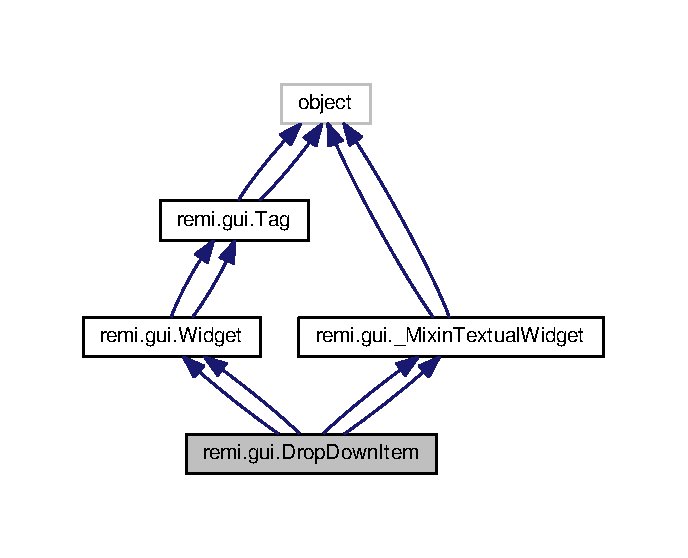
\includegraphics[width=330pt]{d4/d5c/classremi_1_1gui_1_1DropDownItem__inherit__graph}
\end{center}
\end{figure}


Collaboration diagram for remi.\+gui.\+Drop\+Down\+Item\+:
\nopagebreak
\begin{figure}[H]
\begin{center}
\leavevmode
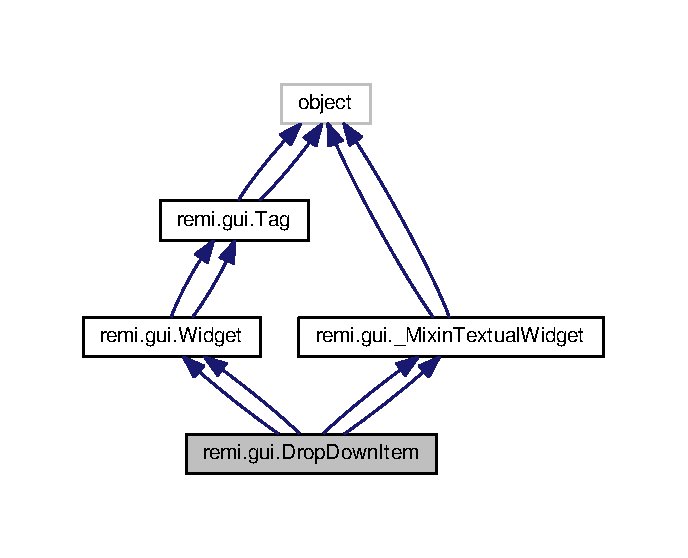
\includegraphics[width=330pt]{d1/da8/classremi_1_1gui_1_1DropDownItem__coll__graph}
\end{center}
\end{figure}
\subsection*{Public Member Functions}
\begin{DoxyCompactItemize}
\item 
def \hyperlink{classremi_1_1gui_1_1DropDownItem_aafd68555ff3bbdf04f8e51d7c2459c93}{\+\_\+\+\_\+init\+\_\+\+\_\+} (self, text, kwargs)
\item 
def \hyperlink{classremi_1_1gui_1_1DropDownItem_a18d8e0ca92616106b1466b8f38946dfc}{set\+\_\+value} (self, text)
\item 
def \hyperlink{classremi_1_1gui_1_1DropDownItem_ac5d1b141b84d264375b5633f86ce87fb}{get\+\_\+value} (self)
\item 
def \hyperlink{classremi_1_1gui_1_1DropDownItem_aafd68555ff3bbdf04f8e51d7c2459c93}{\+\_\+\+\_\+init\+\_\+\+\_\+} (self, text, kwargs)
\item 
def \hyperlink{classremi_1_1gui_1_1DropDownItem_a18d8e0ca92616106b1466b8f38946dfc}{set\+\_\+value} (self, text)
\item 
def \hyperlink{classremi_1_1gui_1_1DropDownItem_ac5d1b141b84d264375b5633f86ce87fb}{get\+\_\+value} (self)
\end{DoxyCompactItemize}
\subsection*{Public Attributes}
\begin{DoxyCompactItemize}
\item 
{\bfseries type}\hypertarget{classremi_1_1gui_1_1DropDownItem_af06466cb76e9481323a9c71c574c0863}{}\label{classremi_1_1gui_1_1DropDownItem_af06466cb76e9481323a9c71c574c0863}

\end{DoxyCompactItemize}
\subsection*{Additional Inherited Members}


\subsection{Detailed Description}
\begin{DoxyVerb}item widget for the DropDown\end{DoxyVerb}
 

\subsection{Constructor \& Destructor Documentation}
\index{remi\+::gui\+::\+Drop\+Down\+Item@{remi\+::gui\+::\+Drop\+Down\+Item}!\+\_\+\+\_\+init\+\_\+\+\_\+@{\+\_\+\+\_\+init\+\_\+\+\_\+}}
\index{\+\_\+\+\_\+init\+\_\+\+\_\+@{\+\_\+\+\_\+init\+\_\+\+\_\+}!remi\+::gui\+::\+Drop\+Down\+Item@{remi\+::gui\+::\+Drop\+Down\+Item}}
\subsubsection[{\texorpdfstring{\+\_\+\+\_\+init\+\_\+\+\_\+(self, text, kwargs)}{__init__(self, text, kwargs)}}]{\setlength{\rightskip}{0pt plus 5cm}def remi.\+gui.\+Drop\+Down\+Item.\+\_\+\+\_\+init\+\_\+\+\_\+ (
\begin{DoxyParamCaption}
\item[{}]{self, }
\item[{}]{text, }
\item[{}]{kwargs}
\end{DoxyParamCaption}
)}\hypertarget{classremi_1_1gui_1_1DropDownItem_aafd68555ff3bbdf04f8e51d7c2459c93}{}\label{classremi_1_1gui_1_1DropDownItem_aafd68555ff3bbdf04f8e51d7c2459c93}
\begin{DoxyVerb}Args:
    kwargs: See Widget.__init__()
\end{DoxyVerb}
 \index{remi\+::gui\+::\+Drop\+Down\+Item@{remi\+::gui\+::\+Drop\+Down\+Item}!\+\_\+\+\_\+init\+\_\+\+\_\+@{\+\_\+\+\_\+init\+\_\+\+\_\+}}
\index{\+\_\+\+\_\+init\+\_\+\+\_\+@{\+\_\+\+\_\+init\+\_\+\+\_\+}!remi\+::gui\+::\+Drop\+Down\+Item@{remi\+::gui\+::\+Drop\+Down\+Item}}
\subsubsection[{\texorpdfstring{\+\_\+\+\_\+init\+\_\+\+\_\+(self, text, kwargs)}{__init__(self, text, kwargs)}}]{\setlength{\rightskip}{0pt plus 5cm}def remi.\+gui.\+Drop\+Down\+Item.\+\_\+\+\_\+init\+\_\+\+\_\+ (
\begin{DoxyParamCaption}
\item[{}]{self, }
\item[{}]{text, }
\item[{}]{kwargs}
\end{DoxyParamCaption}
)}\hypertarget{classremi_1_1gui_1_1DropDownItem_aafd68555ff3bbdf04f8e51d7c2459c93}{}\label{classremi_1_1gui_1_1DropDownItem_aafd68555ff3bbdf04f8e51d7c2459c93}
\begin{DoxyVerb}Args:
    kwargs: See Widget.__init__()
\end{DoxyVerb}
 

\subsection{Member Function Documentation}
\index{remi\+::gui\+::\+Drop\+Down\+Item@{remi\+::gui\+::\+Drop\+Down\+Item}!get\+\_\+value@{get\+\_\+value}}
\index{get\+\_\+value@{get\+\_\+value}!remi\+::gui\+::\+Drop\+Down\+Item@{remi\+::gui\+::\+Drop\+Down\+Item}}
\subsubsection[{\texorpdfstring{get\+\_\+value(self)}{get_value(self)}}]{\setlength{\rightskip}{0pt plus 5cm}def remi.\+gui.\+Drop\+Down\+Item.\+get\+\_\+value (
\begin{DoxyParamCaption}
\item[{}]{self}
\end{DoxyParamCaption}
)}\hypertarget{classremi_1_1gui_1_1DropDownItem_ac5d1b141b84d264375b5633f86ce87fb}{}\label{classremi_1_1gui_1_1DropDownItem_ac5d1b141b84d264375b5633f86ce87fb}
\begin{DoxyVerb}Returns:\end{DoxyVerb}
 \index{remi\+::gui\+::\+Drop\+Down\+Item@{remi\+::gui\+::\+Drop\+Down\+Item}!get\+\_\+value@{get\+\_\+value}}
\index{get\+\_\+value@{get\+\_\+value}!remi\+::gui\+::\+Drop\+Down\+Item@{remi\+::gui\+::\+Drop\+Down\+Item}}
\subsubsection[{\texorpdfstring{get\+\_\+value(self)}{get_value(self)}}]{\setlength{\rightskip}{0pt plus 5cm}def remi.\+gui.\+Drop\+Down\+Item.\+get\+\_\+value (
\begin{DoxyParamCaption}
\item[{}]{self}
\end{DoxyParamCaption}
)}\hypertarget{classremi_1_1gui_1_1DropDownItem_ac5d1b141b84d264375b5633f86ce87fb}{}\label{classremi_1_1gui_1_1DropDownItem_ac5d1b141b84d264375b5633f86ce87fb}
\begin{DoxyVerb}Returns:\end{DoxyVerb}
 \index{remi\+::gui\+::\+Drop\+Down\+Item@{remi\+::gui\+::\+Drop\+Down\+Item}!set\+\_\+value@{set\+\_\+value}}
\index{set\+\_\+value@{set\+\_\+value}!remi\+::gui\+::\+Drop\+Down\+Item@{remi\+::gui\+::\+Drop\+Down\+Item}}
\subsubsection[{\texorpdfstring{set\+\_\+value(self, text)}{set_value(self, text)}}]{\setlength{\rightskip}{0pt plus 5cm}def remi.\+gui.\+Drop\+Down\+Item.\+set\+\_\+value (
\begin{DoxyParamCaption}
\item[{}]{self, }
\item[{}]{text}
\end{DoxyParamCaption}
)}\hypertarget{classremi_1_1gui_1_1DropDownItem_a18d8e0ca92616106b1466b8f38946dfc}{}\label{classremi_1_1gui_1_1DropDownItem_a18d8e0ca92616106b1466b8f38946dfc}
\begin{DoxyVerb}Args:
    text:

Returns:\end{DoxyVerb}
 \index{remi\+::gui\+::\+Drop\+Down\+Item@{remi\+::gui\+::\+Drop\+Down\+Item}!set\+\_\+value@{set\+\_\+value}}
\index{set\+\_\+value@{set\+\_\+value}!remi\+::gui\+::\+Drop\+Down\+Item@{remi\+::gui\+::\+Drop\+Down\+Item}}
\subsubsection[{\texorpdfstring{set\+\_\+value(self, text)}{set_value(self, text)}}]{\setlength{\rightskip}{0pt plus 5cm}def remi.\+gui.\+Drop\+Down\+Item.\+set\+\_\+value (
\begin{DoxyParamCaption}
\item[{}]{self, }
\item[{}]{text}
\end{DoxyParamCaption}
)}\hypertarget{classremi_1_1gui_1_1DropDownItem_a18d8e0ca92616106b1466b8f38946dfc}{}\label{classremi_1_1gui_1_1DropDownItem_a18d8e0ca92616106b1466b8f38946dfc}
\begin{DoxyVerb}Args:
    text:

Returns:\end{DoxyVerb}
 

The documentation for this class was generated from the following file\+:\begin{DoxyCompactItemize}
\item 
Compiled/\+Server/remi/gui.\+py\end{DoxyCompactItemize}

\hypertarget{classmonitor_1_1element}{}\section{monitor.\+element Class Reference}
\label{classmonitor_1_1element}\index{monitor.\+element@{monitor.\+element}}
\subsection*{Public Member Functions}
\begin{DoxyCompactItemize}
\item 
def \hyperlink{classmonitor_1_1element_a2850c0af0e60931936b830a926142117}{\+\_\+\+\_\+init\+\_\+\+\_\+} (self, slot, client, percentage, files, speed, onclick)
\item 
def \hyperlink{classmonitor_1_1element_a4a4a31dae1c21c96d2868eb9ccac98fe}{append\+To} (self, lay)
\item 
def \hyperlink{classmonitor_1_1element_a7d906301ba087ebbc6bc738344a891ce}{update} (self, client, percentage, speed, files)
\item 
def \hyperlink{classmonitor_1_1element_a2850c0af0e60931936b830a926142117}{\+\_\+\+\_\+init\+\_\+\+\_\+} (self, slot, client, percentage, files, speed, onclick)
\item 
def \hyperlink{classmonitor_1_1element_a4a4a31dae1c21c96d2868eb9ccac98fe}{append\+To} (self, lay)
\item 
def \hyperlink{classmonitor_1_1element_a7d906301ba087ebbc6bc738344a891ce}{update} (self, client, percentage, speed, files)
\end{DoxyCompactItemize}
\subsection*{Public Attributes}
\begin{DoxyCompactItemize}
\item 
{\bfseries slot}\hypertarget{classmonitor_1_1element_acfaf72105be355c577e7761fada58d52}{}\label{classmonitor_1_1element_acfaf72105be355c577e7761fada58d52}

\item 
{\bfseries client}\hypertarget{classmonitor_1_1element_ade6af57aec4f6964ba1ac2aa2e36ae87}{}\label{classmonitor_1_1element_ade6af57aec4f6964ba1ac2aa2e36ae87}

\item 
{\bfseries perc}\hypertarget{classmonitor_1_1element_a4b66c40dfa11b631fd48b15193098e4e}{}\label{classmonitor_1_1element_a4b66c40dfa11b631fd48b15193098e4e}

\item 
{\bfseries percentage}\hypertarget{classmonitor_1_1element_a9c6b0bf4d4e227e29a1af667b2ea4e5d}{}\label{classmonitor_1_1element_a9c6b0bf4d4e227e29a1af667b2ea4e5d}

\item 
{\bfseries files}\hypertarget{classmonitor_1_1element_a4ede729a55b617eac98c9c00e9a2024b}{}\label{classmonitor_1_1element_a4ede729a55b617eac98c9c00e9a2024b}

\item 
{\bfseries speed}\hypertarget{classmonitor_1_1element_ac411bb4b1567901178d6807fd2ee2036}{}\label{classmonitor_1_1element_ac411bb4b1567901178d6807fd2ee2036}

\item 
{\bfseries pb}\hypertarget{classmonitor_1_1element_aa6f87019ddf0f0a2a44f4e298285a5e2}{}\label{classmonitor_1_1element_aa6f87019ddf0f0a2a44f4e298285a5e2}

\end{DoxyCompactItemize}


\subsection{Detailed Description}
\begin{DoxyVerb}\end{DoxyVerb}
 

\subsection{Constructor \& Destructor Documentation}
\index{monitor\+::element@{monitor\+::element}!\+\_\+\+\_\+init\+\_\+\+\_\+@{\+\_\+\+\_\+init\+\_\+\+\_\+}}
\index{\+\_\+\+\_\+init\+\_\+\+\_\+@{\+\_\+\+\_\+init\+\_\+\+\_\+}!monitor\+::element@{monitor\+::element}}
\subsubsection[{\texorpdfstring{\+\_\+\+\_\+init\+\_\+\+\_\+(self, slot, client, percentage, files, speed, onclick)}{__init__(self, slot, client, percentage, files, speed, onclick)}}]{\setlength{\rightskip}{0pt plus 5cm}def monitor.\+element.\+\_\+\+\_\+init\+\_\+\+\_\+ (
\begin{DoxyParamCaption}
\item[{}]{self, }
\item[{}]{slot, }
\item[{}]{client, }
\item[{}]{percentage, }
\item[{}]{files, }
\item[{}]{speed, }
\item[{}]{onclick}
\end{DoxyParamCaption}
)}\hypertarget{classmonitor_1_1element_a2850c0af0e60931936b830a926142117}{}\label{classmonitor_1_1element_a2850c0af0e60931936b830a926142117}
\begin{DoxyVerb}Args:
    slot:
    client:
    percentage:
    files:
    speed:
    onclick:
\end{DoxyVerb}
 \index{monitor\+::element@{monitor\+::element}!\+\_\+\+\_\+init\+\_\+\+\_\+@{\+\_\+\+\_\+init\+\_\+\+\_\+}}
\index{\+\_\+\+\_\+init\+\_\+\+\_\+@{\+\_\+\+\_\+init\+\_\+\+\_\+}!monitor\+::element@{monitor\+::element}}
\subsubsection[{\texorpdfstring{\+\_\+\+\_\+init\+\_\+\+\_\+(self, slot, client, percentage, files, speed, onclick)}{__init__(self, slot, client, percentage, files, speed, onclick)}}]{\setlength{\rightskip}{0pt plus 5cm}def monitor.\+element.\+\_\+\+\_\+init\+\_\+\+\_\+ (
\begin{DoxyParamCaption}
\item[{}]{self, }
\item[{}]{slot, }
\item[{}]{client, }
\item[{}]{percentage, }
\item[{}]{files, }
\item[{}]{speed, }
\item[{}]{onclick}
\end{DoxyParamCaption}
)}\hypertarget{classmonitor_1_1element_a2850c0af0e60931936b830a926142117}{}\label{classmonitor_1_1element_a2850c0af0e60931936b830a926142117}
\begin{DoxyVerb}Args:
    slot:
    client:
    percentage:
    files:
    speed:
    onclick:
\end{DoxyVerb}
 

\subsection{Member Function Documentation}
\index{monitor\+::element@{monitor\+::element}!append\+To@{append\+To}}
\index{append\+To@{append\+To}!monitor\+::element@{monitor\+::element}}
\subsubsection[{\texorpdfstring{append\+To(self, lay)}{appendTo(self, lay)}}]{\setlength{\rightskip}{0pt plus 5cm}def monitor.\+element.\+append\+To (
\begin{DoxyParamCaption}
\item[{}]{self, }
\item[{}]{lay}
\end{DoxyParamCaption}
)}\hypertarget{classmonitor_1_1element_a4a4a31dae1c21c96d2868eb9ccac98fe}{}\label{classmonitor_1_1element_a4a4a31dae1c21c96d2868eb9ccac98fe}
\begin{DoxyVerb}Args:
    lay:
\end{DoxyVerb}
 \index{monitor\+::element@{monitor\+::element}!append\+To@{append\+To}}
\index{append\+To@{append\+To}!monitor\+::element@{monitor\+::element}}
\subsubsection[{\texorpdfstring{append\+To(self, lay)}{appendTo(self, lay)}}]{\setlength{\rightskip}{0pt plus 5cm}def monitor.\+element.\+append\+To (
\begin{DoxyParamCaption}
\item[{}]{self, }
\item[{}]{lay}
\end{DoxyParamCaption}
)}\hypertarget{classmonitor_1_1element_a4a4a31dae1c21c96d2868eb9ccac98fe}{}\label{classmonitor_1_1element_a4a4a31dae1c21c96d2868eb9ccac98fe}
\begin{DoxyVerb}Args:
    lay:
\end{DoxyVerb}
 \index{monitor\+::element@{monitor\+::element}!update@{update}}
\index{update@{update}!monitor\+::element@{monitor\+::element}}
\subsubsection[{\texorpdfstring{update(self, client, percentage, speed, files)}{update(self, client, percentage, speed, files)}}]{\setlength{\rightskip}{0pt plus 5cm}def monitor.\+element.\+update (
\begin{DoxyParamCaption}
\item[{}]{self, }
\item[{}]{client, }
\item[{}]{percentage, }
\item[{}]{speed, }
\item[{}]{files}
\end{DoxyParamCaption}
)}\hypertarget{classmonitor_1_1element_a7d906301ba087ebbc6bc738344a891ce}{}\label{classmonitor_1_1element_a7d906301ba087ebbc6bc738344a891ce}
\begin{DoxyVerb}Args:
    client:
    percentage:
    speed:
    files:
\end{DoxyVerb}
 \index{monitor\+::element@{monitor\+::element}!update@{update}}
\index{update@{update}!monitor\+::element@{monitor\+::element}}
\subsubsection[{\texorpdfstring{update(self, client, percentage, speed, files)}{update(self, client, percentage, speed, files)}}]{\setlength{\rightskip}{0pt plus 5cm}def monitor.\+element.\+update (
\begin{DoxyParamCaption}
\item[{}]{self, }
\item[{}]{client, }
\item[{}]{percentage, }
\item[{}]{speed, }
\item[{}]{files}
\end{DoxyParamCaption}
)}\hypertarget{classmonitor_1_1element_a7d906301ba087ebbc6bc738344a891ce}{}\label{classmonitor_1_1element_a7d906301ba087ebbc6bc738344a891ce}
\begin{DoxyVerb}Args:
    client:
    percentage:
    speed:
    files:
\end{DoxyVerb}
 

The documentation for this class was generated from the following file\+:\begin{DoxyCompactItemize}
\item 
Compiled/\+Server/monitor.\+py\end{DoxyCompactItemize}

\hypertarget{classremi_1_1gui_1_1FileDownloader}{}\section{remi.\+gui.\+File\+Downloader Class Reference}
\label{classremi_1_1gui_1_1FileDownloader}\index{remi.\+gui.\+File\+Downloader@{remi.\+gui.\+File\+Downloader}}


Inheritance diagram for remi.\+gui.\+File\+Downloader\+:
\nopagebreak
\begin{figure}[H]
\begin{center}
\leavevmode
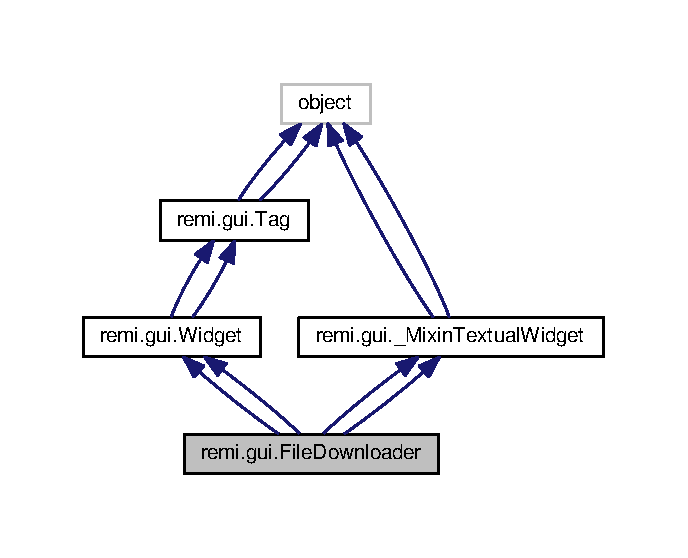
\includegraphics[width=330pt]{d8/dd3/classremi_1_1gui_1_1FileDownloader__inherit__graph}
\end{center}
\end{figure}


Collaboration diagram for remi.\+gui.\+File\+Downloader\+:
\nopagebreak
\begin{figure}[H]
\begin{center}
\leavevmode
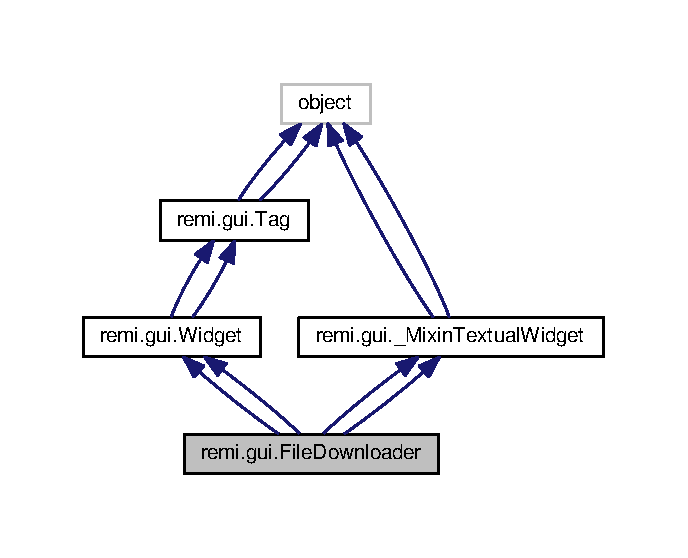
\includegraphics[width=330pt]{d7/de5/classremi_1_1gui_1_1FileDownloader__coll__graph}
\end{center}
\end{figure}
\subsection*{Public Member Functions}
\begin{DoxyCompactItemize}
\item 
def \hyperlink{classremi_1_1gui_1_1FileDownloader_af9c5140851d943c31950bf2dbdb01864}{\+\_\+\+\_\+init\+\_\+\+\_\+} (self, text, filename, path\+\_\+separator=\textquotesingle{}/\textquotesingle{}, kwargs)
\item 
def \hyperlink{classremi_1_1gui_1_1FileDownloader_ad84ce02d7d00e8895735247e3e8f0d5d}{download} (self)
\item 
def \hyperlink{classremi_1_1gui_1_1FileDownloader_af9c5140851d943c31950bf2dbdb01864}{\+\_\+\+\_\+init\+\_\+\+\_\+} (self, text, filename, path\+\_\+separator=\textquotesingle{}/\textquotesingle{}, kwargs)
\item 
def \hyperlink{classremi_1_1gui_1_1FileDownloader_ad84ce02d7d00e8895735247e3e8f0d5d}{download} (self)
\end{DoxyCompactItemize}
\subsection*{Public Attributes}
\begin{DoxyCompactItemize}
\item 
{\bfseries type}\hypertarget{classremi_1_1gui_1_1FileDownloader_acfe49c159fb3a584a911384df0cb17ea}{}\label{classremi_1_1gui_1_1FileDownloader_acfe49c159fb3a584a911384df0cb17ea}

\end{DoxyCompactItemize}
\subsection*{Additional Inherited Members}


\subsection{Detailed Description}
\begin{DoxyVerb}FileDownloader widget. Allows to start a file download.\end{DoxyVerb}
 

\subsection{Constructor \& Destructor Documentation}
\index{remi\+::gui\+::\+File\+Downloader@{remi\+::gui\+::\+File\+Downloader}!\+\_\+\+\_\+init\+\_\+\+\_\+@{\+\_\+\+\_\+init\+\_\+\+\_\+}}
\index{\+\_\+\+\_\+init\+\_\+\+\_\+@{\+\_\+\+\_\+init\+\_\+\+\_\+}!remi\+::gui\+::\+File\+Downloader@{remi\+::gui\+::\+File\+Downloader}}
\subsubsection[{\texorpdfstring{\+\_\+\+\_\+init\+\_\+\+\_\+(self, text, filename, path\+\_\+separator=\textquotesingle{}/\textquotesingle{}, kwargs)}{__init__(self, text, filename, path_separator='/', kwargs)}}]{\setlength{\rightskip}{0pt plus 5cm}def remi.\+gui.\+File\+Downloader.\+\_\+\+\_\+init\+\_\+\+\_\+ (
\begin{DoxyParamCaption}
\item[{}]{self, }
\item[{}]{text, }
\item[{}]{filename, }
\item[{}]{path\+\_\+separator = {\ttfamily \textquotesingle{}/\textquotesingle{}}, }
\item[{}]{kwargs}
\end{DoxyParamCaption}
)}\hypertarget{classremi_1_1gui_1_1FileDownloader_af9c5140851d943c31950bf2dbdb01864}{}\label{classremi_1_1gui_1_1FileDownloader_af9c5140851d943c31950bf2dbdb01864}
\begin{DoxyVerb}Args:
    text:
    filename:
    path_separator:
    kwargs:
\end{DoxyVerb}
 \index{remi\+::gui\+::\+File\+Downloader@{remi\+::gui\+::\+File\+Downloader}!\+\_\+\+\_\+init\+\_\+\+\_\+@{\+\_\+\+\_\+init\+\_\+\+\_\+}}
\index{\+\_\+\+\_\+init\+\_\+\+\_\+@{\+\_\+\+\_\+init\+\_\+\+\_\+}!remi\+::gui\+::\+File\+Downloader@{remi\+::gui\+::\+File\+Downloader}}
\subsubsection[{\texorpdfstring{\+\_\+\+\_\+init\+\_\+\+\_\+(self, text, filename, path\+\_\+separator=\textquotesingle{}/\textquotesingle{}, kwargs)}{__init__(self, text, filename, path_separator='/', kwargs)}}]{\setlength{\rightskip}{0pt plus 5cm}def remi.\+gui.\+File\+Downloader.\+\_\+\+\_\+init\+\_\+\+\_\+ (
\begin{DoxyParamCaption}
\item[{}]{self, }
\item[{}]{text, }
\item[{}]{filename, }
\item[{}]{path\+\_\+separator = {\ttfamily \textquotesingle{}/\textquotesingle{}}, }
\item[{}]{kwargs}
\end{DoxyParamCaption}
)}\hypertarget{classremi_1_1gui_1_1FileDownloader_af9c5140851d943c31950bf2dbdb01864}{}\label{classremi_1_1gui_1_1FileDownloader_af9c5140851d943c31950bf2dbdb01864}
\begin{DoxyVerb}Args:
    text:
    filename:
    path_separator:
    kwargs:
\end{DoxyVerb}
 

\subsection{Member Function Documentation}
\index{remi\+::gui\+::\+File\+Downloader@{remi\+::gui\+::\+File\+Downloader}!download@{download}}
\index{download@{download}!remi\+::gui\+::\+File\+Downloader@{remi\+::gui\+::\+File\+Downloader}}
\subsubsection[{\texorpdfstring{download(self)}{download(self)}}]{\setlength{\rightskip}{0pt plus 5cm}def remi.\+gui.\+File\+Downloader.\+download (
\begin{DoxyParamCaption}
\item[{}]{self}
\end{DoxyParamCaption}
)}\hypertarget{classremi_1_1gui_1_1FileDownloader_ad84ce02d7d00e8895735247e3e8f0d5d}{}\label{classremi_1_1gui_1_1FileDownloader_ad84ce02d7d00e8895735247e3e8f0d5d}
\begin{DoxyVerb}Returns:\end{DoxyVerb}
 \index{remi\+::gui\+::\+File\+Downloader@{remi\+::gui\+::\+File\+Downloader}!download@{download}}
\index{download@{download}!remi\+::gui\+::\+File\+Downloader@{remi\+::gui\+::\+File\+Downloader}}
\subsubsection[{\texorpdfstring{download(self)}{download(self)}}]{\setlength{\rightskip}{0pt plus 5cm}def remi.\+gui.\+File\+Downloader.\+download (
\begin{DoxyParamCaption}
\item[{}]{self}
\end{DoxyParamCaption}
)}\hypertarget{classremi_1_1gui_1_1FileDownloader_ad84ce02d7d00e8895735247e3e8f0d5d}{}\label{classremi_1_1gui_1_1FileDownloader_ad84ce02d7d00e8895735247e3e8f0d5d}
\begin{DoxyVerb}Returns:\end{DoxyVerb}
 

The documentation for this class was generated from the following file\+:\begin{DoxyCompactItemize}
\item 
Compiled/\+Server/remi/gui.\+py\end{DoxyCompactItemize}

\hypertarget{classremi_1_1gui_1_1FileFolderItem}{}\section{remi.\+gui.\+File\+Folder\+Item Class Reference}
\label{classremi_1_1gui_1_1FileFolderItem}\index{remi.\+gui.\+File\+Folder\+Item@{remi.\+gui.\+File\+Folder\+Item}}


Inheritance diagram for remi.\+gui.\+File\+Folder\+Item\+:
\nopagebreak
\begin{figure}[H]
\begin{center}
\leavevmode
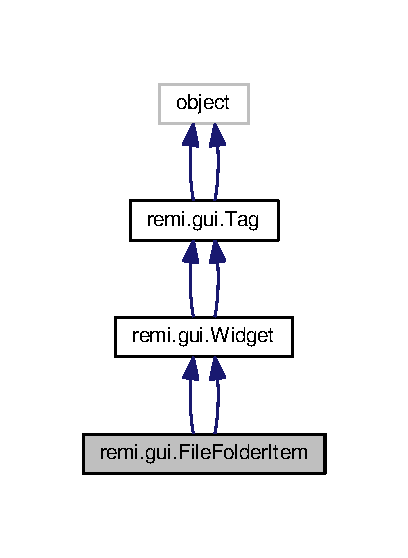
\includegraphics[width=196pt]{dd/de7/classremi_1_1gui_1_1FileFolderItem__inherit__graph}
\end{center}
\end{figure}


Collaboration diagram for remi.\+gui.\+File\+Folder\+Item\+:
\nopagebreak
\begin{figure}[H]
\begin{center}
\leavevmode
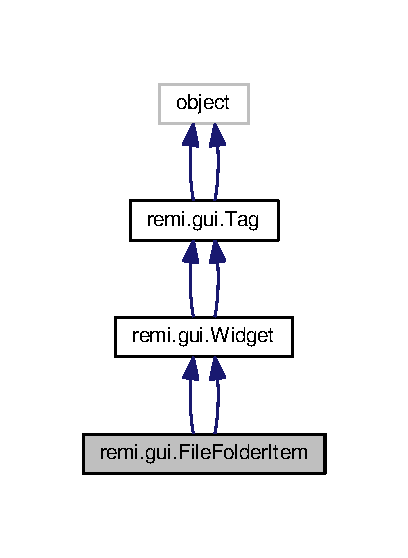
\includegraphics[width=196pt]{d2/da9/classremi_1_1gui_1_1FileFolderItem__coll__graph}
\end{center}
\end{figure}
\subsection*{Public Member Functions}
\begin{DoxyCompactItemize}
\item 
def \hyperlink{classremi_1_1gui_1_1FileFolderItem_afa70c682e41aa230b99f22b656eeb0eb}{\+\_\+\+\_\+init\+\_\+\+\_\+} (self, text, is\+\_\+folder=False, kwargs)
\item 
def \hyperlink{classremi_1_1gui_1_1FileFolderItem_a149faf73abba95f4d381b4ca1fbb3d81}{onclick} (self, widget)
\item 
def \hyperlink{classremi_1_1gui_1_1FileFolderItem_a38f58b3ef28a74d800d01450b6c24a63}{set\+\_\+on\+\_\+click\+\_\+listener} (self, callback, userdata)
\item 
def \hyperlink{classremi_1_1gui_1_1FileFolderItem_afdf1beb86fe8e477b402b36081d2eae6}{set\+\_\+selected} (self, selected)
\item 
def \hyperlink{classremi_1_1gui_1_1FileFolderItem_a45ca805f6423493be1092ee380f4acb5}{onselection} (self, widget)
\item 
def \hyperlink{classremi_1_1gui_1_1FileFolderItem_a9411315a65d4436da290cbdf89a8ee1e}{set\+\_\+on\+\_\+selection\+\_\+listener} (self, callback, userdata)
\item 
def \hyperlink{classremi_1_1gui_1_1FileFolderItem_ac6df7476ed50597c6c3a29a678d105ae}{set\+\_\+text} (self, t)
\item 
def \hyperlink{classremi_1_1gui_1_1FileFolderItem_a8413d5b10fe277bd6b4e40a27e153519}{get\+\_\+text} (self)
\item 
def \hyperlink{classremi_1_1gui_1_1FileFolderItem_afa70c682e41aa230b99f22b656eeb0eb}{\+\_\+\+\_\+init\+\_\+\+\_\+} (self, text, is\+\_\+folder=False, kwargs)
\item 
def \hyperlink{classremi_1_1gui_1_1FileFolderItem_a149faf73abba95f4d381b4ca1fbb3d81}{onclick} (self, widget)
\item 
def \hyperlink{classremi_1_1gui_1_1FileFolderItem_a38f58b3ef28a74d800d01450b6c24a63}{set\+\_\+on\+\_\+click\+\_\+listener} (self, callback, userdata)
\item 
def \hyperlink{classremi_1_1gui_1_1FileFolderItem_afdf1beb86fe8e477b402b36081d2eae6}{set\+\_\+selected} (self, selected)
\item 
def \hyperlink{classremi_1_1gui_1_1FileFolderItem_a45ca805f6423493be1092ee380f4acb5}{onselection} (self, widget)
\item 
def \hyperlink{classremi_1_1gui_1_1FileFolderItem_a9411315a65d4436da290cbdf89a8ee1e}{set\+\_\+on\+\_\+selection\+\_\+listener} (self, callback, userdata)
\item 
def \hyperlink{classremi_1_1gui_1_1FileFolderItem_ac6df7476ed50597c6c3a29a678d105ae}{set\+\_\+text} (self, t)
\item 
def \hyperlink{classremi_1_1gui_1_1FileFolderItem_a8413d5b10fe277bd6b4e40a27e153519}{get\+\_\+text} (self)
\end{DoxyCompactItemize}
\subsection*{Public Attributes}
\begin{DoxyCompactItemize}
\item 
{\bfseries is\+Folder}\hypertarget{classremi_1_1gui_1_1FileFolderItem_a0297b6a33bceb3d4cab83752cbdac36b}{}\label{classremi_1_1gui_1_1FileFolderItem_a0297b6a33bceb3d4cab83752cbdac36b}

\item 
{\bfseries icon}\hypertarget{classremi_1_1gui_1_1FileFolderItem_a45bb7c3ed4793d5cfeecc5e397d7056a}{}\label{classremi_1_1gui_1_1FileFolderItem_a45bb7c3ed4793d5cfeecc5e397d7056a}

\item 
{\bfseries label}\hypertarget{classremi_1_1gui_1_1FileFolderItem_aeccc1c14c3fecc96843dc86e0d62bc24}{}\label{classremi_1_1gui_1_1FileFolderItem_aeccc1c14c3fecc96843dc86e0d62bc24}

\item 
{\bfseries selected}\hypertarget{classremi_1_1gui_1_1FileFolderItem_a8712a71b590ca8b9e648c1d9b75824be}{}\label{classremi_1_1gui_1_1FileFolderItem_a8712a71b590ca8b9e648c1d9b75824be}

\end{DoxyCompactItemize}
\subsection*{Static Public Attributes}
\begin{DoxyCompactItemize}
\item 
string {\bfseries E\+V\+E\+N\+T\+\_\+\+O\+N\+S\+E\+L\+E\+C\+T\+I\+ON} = \textquotesingle{}\hyperlink{classremi_1_1gui_1_1FileFolderItem_a45ca805f6423493be1092ee380f4acb5}{onselection}\textquotesingle{}\hypertarget{classremi_1_1gui_1_1FileFolderItem_a5be6362f0539f9590f429303618682bd}{}\label{classremi_1_1gui_1_1FileFolderItem_a5be6362f0539f9590f429303618682bd}

\end{DoxyCompactItemize}


\subsection{Detailed Description}
\begin{DoxyVerb}FileFolderItem widget for the FileFolderNavigator\end{DoxyVerb}
 

\subsection{Constructor \& Destructor Documentation}
\index{remi\+::gui\+::\+File\+Folder\+Item@{remi\+::gui\+::\+File\+Folder\+Item}!\+\_\+\+\_\+init\+\_\+\+\_\+@{\+\_\+\+\_\+init\+\_\+\+\_\+}}
\index{\+\_\+\+\_\+init\+\_\+\+\_\+@{\+\_\+\+\_\+init\+\_\+\+\_\+}!remi\+::gui\+::\+File\+Folder\+Item@{remi\+::gui\+::\+File\+Folder\+Item}}
\subsubsection[{\texorpdfstring{\+\_\+\+\_\+init\+\_\+\+\_\+(self, text, is\+\_\+folder=\+False, kwargs)}{__init__(self, text, is_folder=False, kwargs)}}]{\setlength{\rightskip}{0pt plus 5cm}def remi.\+gui.\+File\+Folder\+Item.\+\_\+\+\_\+init\+\_\+\+\_\+ (
\begin{DoxyParamCaption}
\item[{}]{self, }
\item[{}]{text, }
\item[{}]{is\+\_\+folder = {\ttfamily False}, }
\item[{}]{kwargs}
\end{DoxyParamCaption}
)}\hypertarget{classremi_1_1gui_1_1FileFolderItem_afa70c682e41aa230b99f22b656eeb0eb}{}\label{classremi_1_1gui_1_1FileFolderItem_afa70c682e41aa230b99f22b656eeb0eb}
\begin{DoxyVerb}Args:
    text:
    is_folder:
    kwargs:
\end{DoxyVerb}
 \index{remi\+::gui\+::\+File\+Folder\+Item@{remi\+::gui\+::\+File\+Folder\+Item}!\+\_\+\+\_\+init\+\_\+\+\_\+@{\+\_\+\+\_\+init\+\_\+\+\_\+}}
\index{\+\_\+\+\_\+init\+\_\+\+\_\+@{\+\_\+\+\_\+init\+\_\+\+\_\+}!remi\+::gui\+::\+File\+Folder\+Item@{remi\+::gui\+::\+File\+Folder\+Item}}
\subsubsection[{\texorpdfstring{\+\_\+\+\_\+init\+\_\+\+\_\+(self, text, is\+\_\+folder=\+False, kwargs)}{__init__(self, text, is_folder=False, kwargs)}}]{\setlength{\rightskip}{0pt plus 5cm}def remi.\+gui.\+File\+Folder\+Item.\+\_\+\+\_\+init\+\_\+\+\_\+ (
\begin{DoxyParamCaption}
\item[{}]{self, }
\item[{}]{text, }
\item[{}]{is\+\_\+folder = {\ttfamily False}, }
\item[{}]{kwargs}
\end{DoxyParamCaption}
)}\hypertarget{classremi_1_1gui_1_1FileFolderItem_afa70c682e41aa230b99f22b656eeb0eb}{}\label{classremi_1_1gui_1_1FileFolderItem_afa70c682e41aa230b99f22b656eeb0eb}
\begin{DoxyVerb}Args:
    text:
    is_folder:
    kwargs:
\end{DoxyVerb}
 

\subsection{Member Function Documentation}
\index{remi\+::gui\+::\+File\+Folder\+Item@{remi\+::gui\+::\+File\+Folder\+Item}!get\+\_\+text@{get\+\_\+text}}
\index{get\+\_\+text@{get\+\_\+text}!remi\+::gui\+::\+File\+Folder\+Item@{remi\+::gui\+::\+File\+Folder\+Item}}
\subsubsection[{\texorpdfstring{get\+\_\+text(self)}{get_text(self)}}]{\setlength{\rightskip}{0pt plus 5cm}def remi.\+gui.\+File\+Folder\+Item.\+get\+\_\+text (
\begin{DoxyParamCaption}
\item[{}]{self}
\end{DoxyParamCaption}
)}\hypertarget{classremi_1_1gui_1_1FileFolderItem_a8413d5b10fe277bd6b4e40a27e153519}{}\label{classremi_1_1gui_1_1FileFolderItem_a8413d5b10fe277bd6b4e40a27e153519}
\begin{DoxyVerb}Returns:\end{DoxyVerb}
 \index{remi\+::gui\+::\+File\+Folder\+Item@{remi\+::gui\+::\+File\+Folder\+Item}!get\+\_\+text@{get\+\_\+text}}
\index{get\+\_\+text@{get\+\_\+text}!remi\+::gui\+::\+File\+Folder\+Item@{remi\+::gui\+::\+File\+Folder\+Item}}
\subsubsection[{\texorpdfstring{get\+\_\+text(self)}{get_text(self)}}]{\setlength{\rightskip}{0pt plus 5cm}def remi.\+gui.\+File\+Folder\+Item.\+get\+\_\+text (
\begin{DoxyParamCaption}
\item[{}]{self}
\end{DoxyParamCaption}
)}\hypertarget{classremi_1_1gui_1_1FileFolderItem_a8413d5b10fe277bd6b4e40a27e153519}{}\label{classremi_1_1gui_1_1FileFolderItem_a8413d5b10fe277bd6b4e40a27e153519}
\begin{DoxyVerb}Returns:\end{DoxyVerb}
 \index{remi\+::gui\+::\+File\+Folder\+Item@{remi\+::gui\+::\+File\+Folder\+Item}!onclick@{onclick}}
\index{onclick@{onclick}!remi\+::gui\+::\+File\+Folder\+Item@{remi\+::gui\+::\+File\+Folder\+Item}}
\subsubsection[{\texorpdfstring{onclick(self, widget)}{onclick(self, widget)}}]{\setlength{\rightskip}{0pt plus 5cm}def remi.\+gui.\+File\+Folder\+Item.\+onclick (
\begin{DoxyParamCaption}
\item[{}]{self, }
\item[{}]{widget}
\end{DoxyParamCaption}
)}\hypertarget{classremi_1_1gui_1_1FileFolderItem_a149faf73abba95f4d381b4ca1fbb3d81}{}\label{classremi_1_1gui_1_1FileFolderItem_a149faf73abba95f4d381b4ca1fbb3d81}
\begin{DoxyVerb}Args:
    widget:

Returns:\end{DoxyVerb}
 \index{remi\+::gui\+::\+File\+Folder\+Item@{remi\+::gui\+::\+File\+Folder\+Item}!onclick@{onclick}}
\index{onclick@{onclick}!remi\+::gui\+::\+File\+Folder\+Item@{remi\+::gui\+::\+File\+Folder\+Item}}
\subsubsection[{\texorpdfstring{onclick(self, widget)}{onclick(self, widget)}}]{\setlength{\rightskip}{0pt plus 5cm}def remi.\+gui.\+File\+Folder\+Item.\+onclick (
\begin{DoxyParamCaption}
\item[{}]{self, }
\item[{}]{widget}
\end{DoxyParamCaption}
)}\hypertarget{classremi_1_1gui_1_1FileFolderItem_a149faf73abba95f4d381b4ca1fbb3d81}{}\label{classremi_1_1gui_1_1FileFolderItem_a149faf73abba95f4d381b4ca1fbb3d81}
\begin{DoxyVerb}Args:
    widget:

Returns:\end{DoxyVerb}
 \index{remi\+::gui\+::\+File\+Folder\+Item@{remi\+::gui\+::\+File\+Folder\+Item}!onselection@{onselection}}
\index{onselection@{onselection}!remi\+::gui\+::\+File\+Folder\+Item@{remi\+::gui\+::\+File\+Folder\+Item}}
\subsubsection[{\texorpdfstring{onselection(self, widget)}{onselection(self, widget)}}]{\setlength{\rightskip}{0pt plus 5cm}def remi.\+gui.\+File\+Folder\+Item.\+onselection (
\begin{DoxyParamCaption}
\item[{}]{self, }
\item[{}]{widget}
\end{DoxyParamCaption}
)}\hypertarget{classremi_1_1gui_1_1FileFolderItem_a45ca805f6423493be1092ee380f4acb5}{}\label{classremi_1_1gui_1_1FileFolderItem_a45ca805f6423493be1092ee380f4acb5}
\begin{DoxyVerb}Args:
    widget:

Returns:\end{DoxyVerb}
 \index{remi\+::gui\+::\+File\+Folder\+Item@{remi\+::gui\+::\+File\+Folder\+Item}!onselection@{onselection}}
\index{onselection@{onselection}!remi\+::gui\+::\+File\+Folder\+Item@{remi\+::gui\+::\+File\+Folder\+Item}}
\subsubsection[{\texorpdfstring{onselection(self, widget)}{onselection(self, widget)}}]{\setlength{\rightskip}{0pt plus 5cm}def remi.\+gui.\+File\+Folder\+Item.\+onselection (
\begin{DoxyParamCaption}
\item[{}]{self, }
\item[{}]{widget}
\end{DoxyParamCaption}
)}\hypertarget{classremi_1_1gui_1_1FileFolderItem_a45ca805f6423493be1092ee380f4acb5}{}\label{classremi_1_1gui_1_1FileFolderItem_a45ca805f6423493be1092ee380f4acb5}
\begin{DoxyVerb}Args:
    widget:

Returns:\end{DoxyVerb}
 \index{remi\+::gui\+::\+File\+Folder\+Item@{remi\+::gui\+::\+File\+Folder\+Item}!set\+\_\+on\+\_\+click\+\_\+listener@{set\+\_\+on\+\_\+click\+\_\+listener}}
\index{set\+\_\+on\+\_\+click\+\_\+listener@{set\+\_\+on\+\_\+click\+\_\+listener}!remi\+::gui\+::\+File\+Folder\+Item@{remi\+::gui\+::\+File\+Folder\+Item}}
\subsubsection[{\texorpdfstring{set\+\_\+on\+\_\+click\+\_\+listener(self, callback, userdata)}{set_on_click_listener(self, callback, userdata)}}]{\setlength{\rightskip}{0pt plus 5cm}def remi.\+gui.\+File\+Folder\+Item.\+set\+\_\+on\+\_\+click\+\_\+listener (
\begin{DoxyParamCaption}
\item[{}]{self, }
\item[{}]{callback, }
\item[{}]{userdata}
\end{DoxyParamCaption}
)}\hypertarget{classremi_1_1gui_1_1FileFolderItem_a38f58b3ef28a74d800d01450b6c24a63}{}\label{classremi_1_1gui_1_1FileFolderItem_a38f58b3ef28a74d800d01450b6c24a63}
\begin{DoxyVerb}Args:
    callback:
    userdata:
\end{DoxyVerb}
 \index{remi\+::gui\+::\+File\+Folder\+Item@{remi\+::gui\+::\+File\+Folder\+Item}!set\+\_\+on\+\_\+click\+\_\+listener@{set\+\_\+on\+\_\+click\+\_\+listener}}
\index{set\+\_\+on\+\_\+click\+\_\+listener@{set\+\_\+on\+\_\+click\+\_\+listener}!remi\+::gui\+::\+File\+Folder\+Item@{remi\+::gui\+::\+File\+Folder\+Item}}
\subsubsection[{\texorpdfstring{set\+\_\+on\+\_\+click\+\_\+listener(self, callback, userdata)}{set_on_click_listener(self, callback, userdata)}}]{\setlength{\rightskip}{0pt plus 5cm}def remi.\+gui.\+File\+Folder\+Item.\+set\+\_\+on\+\_\+click\+\_\+listener (
\begin{DoxyParamCaption}
\item[{}]{self, }
\item[{}]{callback, }
\item[{}]{userdata}
\end{DoxyParamCaption}
)}\hypertarget{classremi_1_1gui_1_1FileFolderItem_a38f58b3ef28a74d800d01450b6c24a63}{}\label{classremi_1_1gui_1_1FileFolderItem_a38f58b3ef28a74d800d01450b6c24a63}
\begin{DoxyVerb}Args:
    callback:
    userdata:
\end{DoxyVerb}
 \index{remi\+::gui\+::\+File\+Folder\+Item@{remi\+::gui\+::\+File\+Folder\+Item}!set\+\_\+on\+\_\+selection\+\_\+listener@{set\+\_\+on\+\_\+selection\+\_\+listener}}
\index{set\+\_\+on\+\_\+selection\+\_\+listener@{set\+\_\+on\+\_\+selection\+\_\+listener}!remi\+::gui\+::\+File\+Folder\+Item@{remi\+::gui\+::\+File\+Folder\+Item}}
\subsubsection[{\texorpdfstring{set\+\_\+on\+\_\+selection\+\_\+listener(self, callback, userdata)}{set_on_selection_listener(self, callback, userdata)}}]{\setlength{\rightskip}{0pt plus 5cm}def remi.\+gui.\+File\+Folder\+Item.\+set\+\_\+on\+\_\+selection\+\_\+listener (
\begin{DoxyParamCaption}
\item[{}]{self, }
\item[{}]{callback, }
\item[{}]{userdata}
\end{DoxyParamCaption}
)}\hypertarget{classremi_1_1gui_1_1FileFolderItem_a9411315a65d4436da290cbdf89a8ee1e}{}\label{classremi_1_1gui_1_1FileFolderItem_a9411315a65d4436da290cbdf89a8ee1e}
\begin{DoxyVerb}Args:
    callback:
    userdata:
\end{DoxyVerb}
 \index{remi\+::gui\+::\+File\+Folder\+Item@{remi\+::gui\+::\+File\+Folder\+Item}!set\+\_\+on\+\_\+selection\+\_\+listener@{set\+\_\+on\+\_\+selection\+\_\+listener}}
\index{set\+\_\+on\+\_\+selection\+\_\+listener@{set\+\_\+on\+\_\+selection\+\_\+listener}!remi\+::gui\+::\+File\+Folder\+Item@{remi\+::gui\+::\+File\+Folder\+Item}}
\subsubsection[{\texorpdfstring{set\+\_\+on\+\_\+selection\+\_\+listener(self, callback, userdata)}{set_on_selection_listener(self, callback, userdata)}}]{\setlength{\rightskip}{0pt plus 5cm}def remi.\+gui.\+File\+Folder\+Item.\+set\+\_\+on\+\_\+selection\+\_\+listener (
\begin{DoxyParamCaption}
\item[{}]{self, }
\item[{}]{callback, }
\item[{}]{userdata}
\end{DoxyParamCaption}
)}\hypertarget{classremi_1_1gui_1_1FileFolderItem_a9411315a65d4436da290cbdf89a8ee1e}{}\label{classremi_1_1gui_1_1FileFolderItem_a9411315a65d4436da290cbdf89a8ee1e}
\begin{DoxyVerb}Args:
    callback:
    userdata:
\end{DoxyVerb}
 \index{remi\+::gui\+::\+File\+Folder\+Item@{remi\+::gui\+::\+File\+Folder\+Item}!set\+\_\+selected@{set\+\_\+selected}}
\index{set\+\_\+selected@{set\+\_\+selected}!remi\+::gui\+::\+File\+Folder\+Item@{remi\+::gui\+::\+File\+Folder\+Item}}
\subsubsection[{\texorpdfstring{set\+\_\+selected(self, selected)}{set_selected(self, selected)}}]{\setlength{\rightskip}{0pt plus 5cm}def remi.\+gui.\+File\+Folder\+Item.\+set\+\_\+selected (
\begin{DoxyParamCaption}
\item[{}]{self, }
\item[{}]{selected}
\end{DoxyParamCaption}
)}\hypertarget{classremi_1_1gui_1_1FileFolderItem_afdf1beb86fe8e477b402b36081d2eae6}{}\label{classremi_1_1gui_1_1FileFolderItem_afdf1beb86fe8e477b402b36081d2eae6}
\begin{DoxyVerb}Args:
    selected:
\end{DoxyVerb}
 \index{remi\+::gui\+::\+File\+Folder\+Item@{remi\+::gui\+::\+File\+Folder\+Item}!set\+\_\+selected@{set\+\_\+selected}}
\index{set\+\_\+selected@{set\+\_\+selected}!remi\+::gui\+::\+File\+Folder\+Item@{remi\+::gui\+::\+File\+Folder\+Item}}
\subsubsection[{\texorpdfstring{set\+\_\+selected(self, selected)}{set_selected(self, selected)}}]{\setlength{\rightskip}{0pt plus 5cm}def remi.\+gui.\+File\+Folder\+Item.\+set\+\_\+selected (
\begin{DoxyParamCaption}
\item[{}]{self, }
\item[{}]{selected}
\end{DoxyParamCaption}
)}\hypertarget{classremi_1_1gui_1_1FileFolderItem_afdf1beb86fe8e477b402b36081d2eae6}{}\label{classremi_1_1gui_1_1FileFolderItem_afdf1beb86fe8e477b402b36081d2eae6}
\begin{DoxyVerb}Args:
    selected:
\end{DoxyVerb}
 \index{remi\+::gui\+::\+File\+Folder\+Item@{remi\+::gui\+::\+File\+Folder\+Item}!set\+\_\+text@{set\+\_\+text}}
\index{set\+\_\+text@{set\+\_\+text}!remi\+::gui\+::\+File\+Folder\+Item@{remi\+::gui\+::\+File\+Folder\+Item}}
\subsubsection[{\texorpdfstring{set\+\_\+text(self, t)}{set_text(self, t)}}]{\setlength{\rightskip}{0pt plus 5cm}def remi.\+gui.\+File\+Folder\+Item.\+set\+\_\+text (
\begin{DoxyParamCaption}
\item[{}]{self, }
\item[{}]{t}
\end{DoxyParamCaption}
)}\hypertarget{classremi_1_1gui_1_1FileFolderItem_ac6df7476ed50597c6c3a29a678d105ae}{}\label{classremi_1_1gui_1_1FileFolderItem_ac6df7476ed50597c6c3a29a678d105ae}
\begin{DoxyVerb}Args:
    t:
\end{DoxyVerb}
 \index{remi\+::gui\+::\+File\+Folder\+Item@{remi\+::gui\+::\+File\+Folder\+Item}!set\+\_\+text@{set\+\_\+text}}
\index{set\+\_\+text@{set\+\_\+text}!remi\+::gui\+::\+File\+Folder\+Item@{remi\+::gui\+::\+File\+Folder\+Item}}
\subsubsection[{\texorpdfstring{set\+\_\+text(self, t)}{set_text(self, t)}}]{\setlength{\rightskip}{0pt plus 5cm}def remi.\+gui.\+File\+Folder\+Item.\+set\+\_\+text (
\begin{DoxyParamCaption}
\item[{}]{self, }
\item[{}]{t}
\end{DoxyParamCaption}
)}\hypertarget{classremi_1_1gui_1_1FileFolderItem_ac6df7476ed50597c6c3a29a678d105ae}{}\label{classremi_1_1gui_1_1FileFolderItem_ac6df7476ed50597c6c3a29a678d105ae}
\begin{DoxyVerb}Args:
    t:
\end{DoxyVerb}
 

The documentation for this class was generated from the following file\+:\begin{DoxyCompactItemize}
\item 
Compiled/\+Server/remi/gui.\+py\end{DoxyCompactItemize}

\hypertarget{classremi_1_1gui_1_1FileFolderNavigator}{}\section{remi.\+gui.\+File\+Folder\+Navigator Class Reference}
\label{classremi_1_1gui_1_1FileFolderNavigator}\index{remi.\+gui.\+File\+Folder\+Navigator@{remi.\+gui.\+File\+Folder\+Navigator}}


Inheritance diagram for remi.\+gui.\+File\+Folder\+Navigator\+:
\nopagebreak
\begin{figure}[H]
\begin{center}
\leavevmode
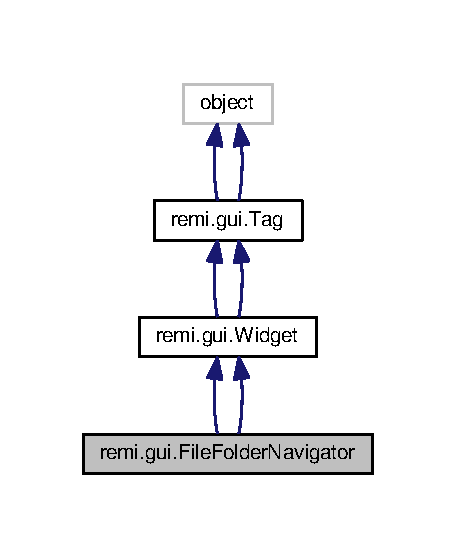
\includegraphics[width=219pt]{d6/d18/classremi_1_1gui_1_1FileFolderNavigator__inherit__graph}
\end{center}
\end{figure}


Collaboration diagram for remi.\+gui.\+File\+Folder\+Navigator\+:
\nopagebreak
\begin{figure}[H]
\begin{center}
\leavevmode
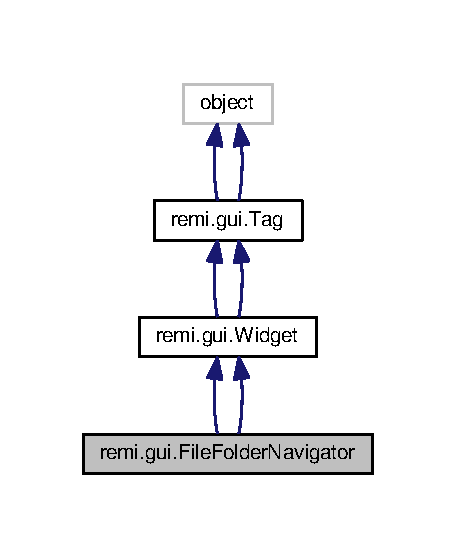
\includegraphics[width=219pt]{d5/dd7/classremi_1_1gui_1_1FileFolderNavigator__coll__graph}
\end{center}
\end{figure}
\subsection*{Public Member Functions}
\begin{DoxyCompactItemize}
\item 
def \hyperlink{classremi_1_1gui_1_1FileFolderNavigator_a4686cb9331de748dc868b41ae81177f2}{\+\_\+\+\_\+init\+\_\+\+\_\+} (self, multiple\+\_\+selection, selection\+\_\+folder, allow\+\_\+file\+\_\+selection, allow\+\_\+folder\+\_\+selection, kwargs)
\item 
def \hyperlink{classremi_1_1gui_1_1FileFolderNavigator_a3996d5d90e883fb51744fd09948a2186}{get\+\_\+selection\+\_\+list} (self)
\item 
def \hyperlink{classremi_1_1gui_1_1FileFolderNavigator_a6bb12a130335b050647c24017a6055ba}{populate\+\_\+folder\+\_\+items} (self, directory)
\item 
def \hyperlink{classremi_1_1gui_1_1FileFolderNavigator_a5f64299c264af76267546db5296e5940}{dir\+\_\+go\+\_\+back} (self, widget)
\item 
def \hyperlink{classremi_1_1gui_1_1FileFolderNavigator_a7c1e11569c677f06a30fe065efff9b0f}{dir\+\_\+go} (self, widget)
\item 
def \hyperlink{classremi_1_1gui_1_1FileFolderNavigator_a68e64ee0d851e42e48e439932d6bd11b}{chdir} (self, directory)
\item 
def \hyperlink{classremi_1_1gui_1_1FileFolderNavigator_a11d7c3e56019d6caada880c1304170dc}{on\+\_\+folder\+\_\+item\+\_\+selected} (self, folderitem)
\item 
def \hyperlink{classremi_1_1gui_1_1FileFolderNavigator_a302e4113c2b897bbf0670dba485e6be9}{on\+\_\+folder\+\_\+item\+\_\+click} (self, folderitem)
\item 
def \hyperlink{classremi_1_1gui_1_1FileFolderNavigator_af2515489544b9461352a6901a872b695}{get\+\_\+selected\+\_\+filefolders} (self)
\item 
def \hyperlink{classremi_1_1gui_1_1FileFolderNavigator_a4686cb9331de748dc868b41ae81177f2}{\+\_\+\+\_\+init\+\_\+\+\_\+} (self, multiple\+\_\+selection, selection\+\_\+folder, allow\+\_\+file\+\_\+selection, allow\+\_\+folder\+\_\+selection, kwargs)
\item 
def \hyperlink{classremi_1_1gui_1_1FileFolderNavigator_a3996d5d90e883fb51744fd09948a2186}{get\+\_\+selection\+\_\+list} (self)
\item 
def \hyperlink{classremi_1_1gui_1_1FileFolderNavigator_a6bb12a130335b050647c24017a6055ba}{populate\+\_\+folder\+\_\+items} (self, directory)
\item 
def \hyperlink{classremi_1_1gui_1_1FileFolderNavigator_a5f64299c264af76267546db5296e5940}{dir\+\_\+go\+\_\+back} (self, widget)
\item 
def \hyperlink{classremi_1_1gui_1_1FileFolderNavigator_a7c1e11569c677f06a30fe065efff9b0f}{dir\+\_\+go} (self, widget)
\item 
def \hyperlink{classremi_1_1gui_1_1FileFolderNavigator_a68e64ee0d851e42e48e439932d6bd11b}{chdir} (self, directory)
\item 
def \hyperlink{classremi_1_1gui_1_1FileFolderNavigator_a11d7c3e56019d6caada880c1304170dc}{on\+\_\+folder\+\_\+item\+\_\+selected} (self, folderitem)
\item 
def \hyperlink{classremi_1_1gui_1_1FileFolderNavigator_a302e4113c2b897bbf0670dba485e6be9}{on\+\_\+folder\+\_\+item\+\_\+click} (self, folderitem)
\item 
def \hyperlink{classremi_1_1gui_1_1FileFolderNavigator_af2515489544b9461352a6901a872b695}{get\+\_\+selected\+\_\+filefolders} (self)
\end{DoxyCompactItemize}
\subsection*{Public Attributes}
\begin{DoxyCompactItemize}
\item 
{\bfseries multiple\+\_\+selection}\hypertarget{classremi_1_1gui_1_1FileFolderNavigator_a29766cad9766b0a22ec81b3b6eed8dda}{}\label{classremi_1_1gui_1_1FileFolderNavigator_a29766cad9766b0a22ec81b3b6eed8dda}

\item 
{\bfseries allow\+\_\+file\+\_\+selection}\hypertarget{classremi_1_1gui_1_1FileFolderNavigator_a8ee6a5c6f7ee54446582dd8a65739e62}{}\label{classremi_1_1gui_1_1FileFolderNavigator_a8ee6a5c6f7ee54446582dd8a65739e62}

\item 
{\bfseries allow\+\_\+folder\+\_\+selection}\hypertarget{classremi_1_1gui_1_1FileFolderNavigator_aad0b4bd91ea56c31622c4d4a643399dd}{}\label{classremi_1_1gui_1_1FileFolderNavigator_aad0b4bd91ea56c31622c4d4a643399dd}

\item 
{\bfseries selectionlist}\hypertarget{classremi_1_1gui_1_1FileFolderNavigator_a4b7bcb9f0ae3d50ed190234bb77d7546}{}\label{classremi_1_1gui_1_1FileFolderNavigator_a4b7bcb9f0ae3d50ed190234bb77d7546}

\item 
{\bfseries controls\+Container}\hypertarget{classremi_1_1gui_1_1FileFolderNavigator_a29dd4a3848da516f635b727a3d35a2e5}{}\label{classremi_1_1gui_1_1FileFolderNavigator_a29dd4a3848da516f635b727a3d35a2e5}

\item 
{\bfseries control\+Back}\hypertarget{classremi_1_1gui_1_1FileFolderNavigator_ac1de65dd68349858505e92b03910a656}{}\label{classremi_1_1gui_1_1FileFolderNavigator_ac1de65dd68349858505e92b03910a656}

\item 
{\bfseries control\+Go}\hypertarget{classremi_1_1gui_1_1FileFolderNavigator_a2361623c6dd1a7162b1b526873ebe3b2}{}\label{classremi_1_1gui_1_1FileFolderNavigator_a2361623c6dd1a7162b1b526873ebe3b2}

\item 
{\bfseries path\+Editor}\hypertarget{classremi_1_1gui_1_1FileFolderNavigator_a296be0e6e448a40b4777450c2060e602}{}\label{classremi_1_1gui_1_1FileFolderNavigator_a296be0e6e448a40b4777450c2060e602}

\item 
{\bfseries item\+Container}\hypertarget{classremi_1_1gui_1_1FileFolderNavigator_aba857c4078b9900bbda74839639fc205}{}\label{classremi_1_1gui_1_1FileFolderNavigator_aba857c4078b9900bbda74839639fc205}

\item 
{\bfseries folder\+Items}\hypertarget{classremi_1_1gui_1_1FileFolderNavigator_a946acd59781879b3b44b40d1e3b68bc0}{}\label{classremi_1_1gui_1_1FileFolderNavigator_a946acd59781879b3b44b40d1e3b68bc0}

\end{DoxyCompactItemize}
\subsection*{Additional Inherited Members}


\subsection{Detailed Description}
\begin{DoxyVerb}FileFolderNavigator widget.\end{DoxyVerb}
 

\subsection{Constructor \& Destructor Documentation}
\index{remi\+::gui\+::\+File\+Folder\+Navigator@{remi\+::gui\+::\+File\+Folder\+Navigator}!\+\_\+\+\_\+init\+\_\+\+\_\+@{\+\_\+\+\_\+init\+\_\+\+\_\+}}
\index{\+\_\+\+\_\+init\+\_\+\+\_\+@{\+\_\+\+\_\+init\+\_\+\+\_\+}!remi\+::gui\+::\+File\+Folder\+Navigator@{remi\+::gui\+::\+File\+Folder\+Navigator}}
\subsubsection[{\texorpdfstring{\+\_\+\+\_\+init\+\_\+\+\_\+(self, multiple\+\_\+selection, selection\+\_\+folder, allow\+\_\+file\+\_\+selection, allow\+\_\+folder\+\_\+selection, kwargs)}{__init__(self, multiple_selection, selection_folder, allow_file_selection, allow_folder_selection, kwargs)}}]{\setlength{\rightskip}{0pt plus 5cm}def remi.\+gui.\+File\+Folder\+Navigator.\+\_\+\+\_\+init\+\_\+\+\_\+ (
\begin{DoxyParamCaption}
\item[{}]{self, }
\item[{}]{multiple\+\_\+selection, }
\item[{}]{selection\+\_\+folder, }
\item[{}]{allow\+\_\+file\+\_\+selection, }
\item[{}]{allow\+\_\+folder\+\_\+selection, }
\item[{}]{kwargs}
\end{DoxyParamCaption}
)}\hypertarget{classremi_1_1gui_1_1FileFolderNavigator_a4686cb9331de748dc868b41ae81177f2}{}\label{classremi_1_1gui_1_1FileFolderNavigator_a4686cb9331de748dc868b41ae81177f2}
\begin{DoxyVerb}Args:
    multiple_selection:
    selection_folder:
    allow_file_selection:
    allow_folder_selection:
    kwargs:
\end{DoxyVerb}
 \index{remi\+::gui\+::\+File\+Folder\+Navigator@{remi\+::gui\+::\+File\+Folder\+Navigator}!\+\_\+\+\_\+init\+\_\+\+\_\+@{\+\_\+\+\_\+init\+\_\+\+\_\+}}
\index{\+\_\+\+\_\+init\+\_\+\+\_\+@{\+\_\+\+\_\+init\+\_\+\+\_\+}!remi\+::gui\+::\+File\+Folder\+Navigator@{remi\+::gui\+::\+File\+Folder\+Navigator}}
\subsubsection[{\texorpdfstring{\+\_\+\+\_\+init\+\_\+\+\_\+(self, multiple\+\_\+selection, selection\+\_\+folder, allow\+\_\+file\+\_\+selection, allow\+\_\+folder\+\_\+selection, kwargs)}{__init__(self, multiple_selection, selection_folder, allow_file_selection, allow_folder_selection, kwargs)}}]{\setlength{\rightskip}{0pt plus 5cm}def remi.\+gui.\+File\+Folder\+Navigator.\+\_\+\+\_\+init\+\_\+\+\_\+ (
\begin{DoxyParamCaption}
\item[{}]{self, }
\item[{}]{multiple\+\_\+selection, }
\item[{}]{selection\+\_\+folder, }
\item[{}]{allow\+\_\+file\+\_\+selection, }
\item[{}]{allow\+\_\+folder\+\_\+selection, }
\item[{}]{kwargs}
\end{DoxyParamCaption}
)}\hypertarget{classremi_1_1gui_1_1FileFolderNavigator_a4686cb9331de748dc868b41ae81177f2}{}\label{classremi_1_1gui_1_1FileFolderNavigator_a4686cb9331de748dc868b41ae81177f2}
\begin{DoxyVerb}Args:
    multiple_selection:
    selection_folder:
    allow_file_selection:
    allow_folder_selection:
    kwargs:
\end{DoxyVerb}
 

\subsection{Member Function Documentation}
\index{remi\+::gui\+::\+File\+Folder\+Navigator@{remi\+::gui\+::\+File\+Folder\+Navigator}!chdir@{chdir}}
\index{chdir@{chdir}!remi\+::gui\+::\+File\+Folder\+Navigator@{remi\+::gui\+::\+File\+Folder\+Navigator}}
\subsubsection[{\texorpdfstring{chdir(self, directory)}{chdir(self, directory)}}]{\setlength{\rightskip}{0pt plus 5cm}def remi.\+gui.\+File\+Folder\+Navigator.\+chdir (
\begin{DoxyParamCaption}
\item[{}]{self, }
\item[{}]{directory}
\end{DoxyParamCaption}
)}\hypertarget{classremi_1_1gui_1_1FileFolderNavigator_a68e64ee0d851e42e48e439932d6bd11b}{}\label{classremi_1_1gui_1_1FileFolderNavigator_a68e64ee0d851e42e48e439932d6bd11b}
\begin{DoxyVerb}Args:
    directory:
\end{DoxyVerb}
 \index{remi\+::gui\+::\+File\+Folder\+Navigator@{remi\+::gui\+::\+File\+Folder\+Navigator}!chdir@{chdir}}
\index{chdir@{chdir}!remi\+::gui\+::\+File\+Folder\+Navigator@{remi\+::gui\+::\+File\+Folder\+Navigator}}
\subsubsection[{\texorpdfstring{chdir(self, directory)}{chdir(self, directory)}}]{\setlength{\rightskip}{0pt plus 5cm}def remi.\+gui.\+File\+Folder\+Navigator.\+chdir (
\begin{DoxyParamCaption}
\item[{}]{self, }
\item[{}]{directory}
\end{DoxyParamCaption}
)}\hypertarget{classremi_1_1gui_1_1FileFolderNavigator_a68e64ee0d851e42e48e439932d6bd11b}{}\label{classremi_1_1gui_1_1FileFolderNavigator_a68e64ee0d851e42e48e439932d6bd11b}
\begin{DoxyVerb}Args:
    directory:
\end{DoxyVerb}
 \index{remi\+::gui\+::\+File\+Folder\+Navigator@{remi\+::gui\+::\+File\+Folder\+Navigator}!dir\+\_\+go@{dir\+\_\+go}}
\index{dir\+\_\+go@{dir\+\_\+go}!remi\+::gui\+::\+File\+Folder\+Navigator@{remi\+::gui\+::\+File\+Folder\+Navigator}}
\subsubsection[{\texorpdfstring{dir\+\_\+go(self, widget)}{dir_go(self, widget)}}]{\setlength{\rightskip}{0pt plus 5cm}def remi.\+gui.\+File\+Folder\+Navigator.\+dir\+\_\+go (
\begin{DoxyParamCaption}
\item[{}]{self, }
\item[{}]{widget}
\end{DoxyParamCaption}
)}\hypertarget{classremi_1_1gui_1_1FileFolderNavigator_a7c1e11569c677f06a30fe065efff9b0f}{}\label{classremi_1_1gui_1_1FileFolderNavigator_a7c1e11569c677f06a30fe065efff9b0f}
\begin{DoxyVerb}Args:
    widget:
\end{DoxyVerb}
 \index{remi\+::gui\+::\+File\+Folder\+Navigator@{remi\+::gui\+::\+File\+Folder\+Navigator}!dir\+\_\+go@{dir\+\_\+go}}
\index{dir\+\_\+go@{dir\+\_\+go}!remi\+::gui\+::\+File\+Folder\+Navigator@{remi\+::gui\+::\+File\+Folder\+Navigator}}
\subsubsection[{\texorpdfstring{dir\+\_\+go(self, widget)}{dir_go(self, widget)}}]{\setlength{\rightskip}{0pt plus 5cm}def remi.\+gui.\+File\+Folder\+Navigator.\+dir\+\_\+go (
\begin{DoxyParamCaption}
\item[{}]{self, }
\item[{}]{widget}
\end{DoxyParamCaption}
)}\hypertarget{classremi_1_1gui_1_1FileFolderNavigator_a7c1e11569c677f06a30fe065efff9b0f}{}\label{classremi_1_1gui_1_1FileFolderNavigator_a7c1e11569c677f06a30fe065efff9b0f}
\begin{DoxyVerb}Args:
    widget:
\end{DoxyVerb}
 \index{remi\+::gui\+::\+File\+Folder\+Navigator@{remi\+::gui\+::\+File\+Folder\+Navigator}!dir\+\_\+go\+\_\+back@{dir\+\_\+go\+\_\+back}}
\index{dir\+\_\+go\+\_\+back@{dir\+\_\+go\+\_\+back}!remi\+::gui\+::\+File\+Folder\+Navigator@{remi\+::gui\+::\+File\+Folder\+Navigator}}
\subsubsection[{\texorpdfstring{dir\+\_\+go\+\_\+back(self, widget)}{dir_go_back(self, widget)}}]{\setlength{\rightskip}{0pt plus 5cm}def remi.\+gui.\+File\+Folder\+Navigator.\+dir\+\_\+go\+\_\+back (
\begin{DoxyParamCaption}
\item[{}]{self, }
\item[{}]{widget}
\end{DoxyParamCaption}
)}\hypertarget{classremi_1_1gui_1_1FileFolderNavigator_a5f64299c264af76267546db5296e5940}{}\label{classremi_1_1gui_1_1FileFolderNavigator_a5f64299c264af76267546db5296e5940}
\begin{DoxyVerb}Args:
    widget:
\end{DoxyVerb}
 \index{remi\+::gui\+::\+File\+Folder\+Navigator@{remi\+::gui\+::\+File\+Folder\+Navigator}!dir\+\_\+go\+\_\+back@{dir\+\_\+go\+\_\+back}}
\index{dir\+\_\+go\+\_\+back@{dir\+\_\+go\+\_\+back}!remi\+::gui\+::\+File\+Folder\+Navigator@{remi\+::gui\+::\+File\+Folder\+Navigator}}
\subsubsection[{\texorpdfstring{dir\+\_\+go\+\_\+back(self, widget)}{dir_go_back(self, widget)}}]{\setlength{\rightskip}{0pt plus 5cm}def remi.\+gui.\+File\+Folder\+Navigator.\+dir\+\_\+go\+\_\+back (
\begin{DoxyParamCaption}
\item[{}]{self, }
\item[{}]{widget}
\end{DoxyParamCaption}
)}\hypertarget{classremi_1_1gui_1_1FileFolderNavigator_a5f64299c264af76267546db5296e5940}{}\label{classremi_1_1gui_1_1FileFolderNavigator_a5f64299c264af76267546db5296e5940}
\begin{DoxyVerb}Args:
    widget:
\end{DoxyVerb}
 \index{remi\+::gui\+::\+File\+Folder\+Navigator@{remi\+::gui\+::\+File\+Folder\+Navigator}!get\+\_\+selected\+\_\+filefolders@{get\+\_\+selected\+\_\+filefolders}}
\index{get\+\_\+selected\+\_\+filefolders@{get\+\_\+selected\+\_\+filefolders}!remi\+::gui\+::\+File\+Folder\+Navigator@{remi\+::gui\+::\+File\+Folder\+Navigator}}
\subsubsection[{\texorpdfstring{get\+\_\+selected\+\_\+filefolders(self)}{get_selected_filefolders(self)}}]{\setlength{\rightskip}{0pt plus 5cm}def remi.\+gui.\+File\+Folder\+Navigator.\+get\+\_\+selected\+\_\+filefolders (
\begin{DoxyParamCaption}
\item[{}]{self}
\end{DoxyParamCaption}
)}\hypertarget{classremi_1_1gui_1_1FileFolderNavigator_af2515489544b9461352a6901a872b695}{}\label{classremi_1_1gui_1_1FileFolderNavigator_af2515489544b9461352a6901a872b695}
\begin{DoxyVerb}Returns:\end{DoxyVerb}
 \index{remi\+::gui\+::\+File\+Folder\+Navigator@{remi\+::gui\+::\+File\+Folder\+Navigator}!get\+\_\+selected\+\_\+filefolders@{get\+\_\+selected\+\_\+filefolders}}
\index{get\+\_\+selected\+\_\+filefolders@{get\+\_\+selected\+\_\+filefolders}!remi\+::gui\+::\+File\+Folder\+Navigator@{remi\+::gui\+::\+File\+Folder\+Navigator}}
\subsubsection[{\texorpdfstring{get\+\_\+selected\+\_\+filefolders(self)}{get_selected_filefolders(self)}}]{\setlength{\rightskip}{0pt plus 5cm}def remi.\+gui.\+File\+Folder\+Navigator.\+get\+\_\+selected\+\_\+filefolders (
\begin{DoxyParamCaption}
\item[{}]{self}
\end{DoxyParamCaption}
)}\hypertarget{classremi_1_1gui_1_1FileFolderNavigator_af2515489544b9461352a6901a872b695}{}\label{classremi_1_1gui_1_1FileFolderNavigator_af2515489544b9461352a6901a872b695}
\begin{DoxyVerb}Returns:\end{DoxyVerb}
 \index{remi\+::gui\+::\+File\+Folder\+Navigator@{remi\+::gui\+::\+File\+Folder\+Navigator}!get\+\_\+selection\+\_\+list@{get\+\_\+selection\+\_\+list}}
\index{get\+\_\+selection\+\_\+list@{get\+\_\+selection\+\_\+list}!remi\+::gui\+::\+File\+Folder\+Navigator@{remi\+::gui\+::\+File\+Folder\+Navigator}}
\subsubsection[{\texorpdfstring{get\+\_\+selection\+\_\+list(self)}{get_selection_list(self)}}]{\setlength{\rightskip}{0pt plus 5cm}def remi.\+gui.\+File\+Folder\+Navigator.\+get\+\_\+selection\+\_\+list (
\begin{DoxyParamCaption}
\item[{}]{self}
\end{DoxyParamCaption}
)}\hypertarget{classremi_1_1gui_1_1FileFolderNavigator_a3996d5d90e883fb51744fd09948a2186}{}\label{classremi_1_1gui_1_1FileFolderNavigator_a3996d5d90e883fb51744fd09948a2186}
\begin{DoxyVerb}Returns:\end{DoxyVerb}
 \index{remi\+::gui\+::\+File\+Folder\+Navigator@{remi\+::gui\+::\+File\+Folder\+Navigator}!get\+\_\+selection\+\_\+list@{get\+\_\+selection\+\_\+list}}
\index{get\+\_\+selection\+\_\+list@{get\+\_\+selection\+\_\+list}!remi\+::gui\+::\+File\+Folder\+Navigator@{remi\+::gui\+::\+File\+Folder\+Navigator}}
\subsubsection[{\texorpdfstring{get\+\_\+selection\+\_\+list(self)}{get_selection_list(self)}}]{\setlength{\rightskip}{0pt plus 5cm}def remi.\+gui.\+File\+Folder\+Navigator.\+get\+\_\+selection\+\_\+list (
\begin{DoxyParamCaption}
\item[{}]{self}
\end{DoxyParamCaption}
)}\hypertarget{classremi_1_1gui_1_1FileFolderNavigator_a3996d5d90e883fb51744fd09948a2186}{}\label{classremi_1_1gui_1_1FileFolderNavigator_a3996d5d90e883fb51744fd09948a2186}
\begin{DoxyVerb}Returns:\end{DoxyVerb}
 \index{remi\+::gui\+::\+File\+Folder\+Navigator@{remi\+::gui\+::\+File\+Folder\+Navigator}!on\+\_\+folder\+\_\+item\+\_\+click@{on\+\_\+folder\+\_\+item\+\_\+click}}
\index{on\+\_\+folder\+\_\+item\+\_\+click@{on\+\_\+folder\+\_\+item\+\_\+click}!remi\+::gui\+::\+File\+Folder\+Navigator@{remi\+::gui\+::\+File\+Folder\+Navigator}}
\subsubsection[{\texorpdfstring{on\+\_\+folder\+\_\+item\+\_\+click(self, folderitem)}{on_folder_item_click(self, folderitem)}}]{\setlength{\rightskip}{0pt plus 5cm}def remi.\+gui.\+File\+Folder\+Navigator.\+on\+\_\+folder\+\_\+item\+\_\+click (
\begin{DoxyParamCaption}
\item[{}]{self, }
\item[{}]{folderitem}
\end{DoxyParamCaption}
)}\hypertarget{classremi_1_1gui_1_1FileFolderNavigator_a302e4113c2b897bbf0670dba485e6be9}{}\label{classremi_1_1gui_1_1FileFolderNavigator_a302e4113c2b897bbf0670dba485e6be9}
\begin{DoxyVerb}Args:
    folderitem:
\end{DoxyVerb}
 \index{remi\+::gui\+::\+File\+Folder\+Navigator@{remi\+::gui\+::\+File\+Folder\+Navigator}!on\+\_\+folder\+\_\+item\+\_\+click@{on\+\_\+folder\+\_\+item\+\_\+click}}
\index{on\+\_\+folder\+\_\+item\+\_\+click@{on\+\_\+folder\+\_\+item\+\_\+click}!remi\+::gui\+::\+File\+Folder\+Navigator@{remi\+::gui\+::\+File\+Folder\+Navigator}}
\subsubsection[{\texorpdfstring{on\+\_\+folder\+\_\+item\+\_\+click(self, folderitem)}{on_folder_item_click(self, folderitem)}}]{\setlength{\rightskip}{0pt plus 5cm}def remi.\+gui.\+File\+Folder\+Navigator.\+on\+\_\+folder\+\_\+item\+\_\+click (
\begin{DoxyParamCaption}
\item[{}]{self, }
\item[{}]{folderitem}
\end{DoxyParamCaption}
)}\hypertarget{classremi_1_1gui_1_1FileFolderNavigator_a302e4113c2b897bbf0670dba485e6be9}{}\label{classremi_1_1gui_1_1FileFolderNavigator_a302e4113c2b897bbf0670dba485e6be9}
\begin{DoxyVerb}Args:
    folderitem:
\end{DoxyVerb}
 \index{remi\+::gui\+::\+File\+Folder\+Navigator@{remi\+::gui\+::\+File\+Folder\+Navigator}!on\+\_\+folder\+\_\+item\+\_\+selected@{on\+\_\+folder\+\_\+item\+\_\+selected}}
\index{on\+\_\+folder\+\_\+item\+\_\+selected@{on\+\_\+folder\+\_\+item\+\_\+selected}!remi\+::gui\+::\+File\+Folder\+Navigator@{remi\+::gui\+::\+File\+Folder\+Navigator}}
\subsubsection[{\texorpdfstring{on\+\_\+folder\+\_\+item\+\_\+selected(self, folderitem)}{on_folder_item_selected(self, folderitem)}}]{\setlength{\rightskip}{0pt plus 5cm}def remi.\+gui.\+File\+Folder\+Navigator.\+on\+\_\+folder\+\_\+item\+\_\+selected (
\begin{DoxyParamCaption}
\item[{}]{self, }
\item[{}]{folderitem}
\end{DoxyParamCaption}
)}\hypertarget{classremi_1_1gui_1_1FileFolderNavigator_a11d7c3e56019d6caada880c1304170dc}{}\label{classremi_1_1gui_1_1FileFolderNavigator_a11d7c3e56019d6caada880c1304170dc}
\begin{DoxyVerb}Args:
    folderitem:

Returns:\end{DoxyVerb}
 \index{remi\+::gui\+::\+File\+Folder\+Navigator@{remi\+::gui\+::\+File\+Folder\+Navigator}!on\+\_\+folder\+\_\+item\+\_\+selected@{on\+\_\+folder\+\_\+item\+\_\+selected}}
\index{on\+\_\+folder\+\_\+item\+\_\+selected@{on\+\_\+folder\+\_\+item\+\_\+selected}!remi\+::gui\+::\+File\+Folder\+Navigator@{remi\+::gui\+::\+File\+Folder\+Navigator}}
\subsubsection[{\texorpdfstring{on\+\_\+folder\+\_\+item\+\_\+selected(self, folderitem)}{on_folder_item_selected(self, folderitem)}}]{\setlength{\rightskip}{0pt plus 5cm}def remi.\+gui.\+File\+Folder\+Navigator.\+on\+\_\+folder\+\_\+item\+\_\+selected (
\begin{DoxyParamCaption}
\item[{}]{self, }
\item[{}]{folderitem}
\end{DoxyParamCaption}
)}\hypertarget{classremi_1_1gui_1_1FileFolderNavigator_a11d7c3e56019d6caada880c1304170dc}{}\label{classremi_1_1gui_1_1FileFolderNavigator_a11d7c3e56019d6caada880c1304170dc}
\begin{DoxyVerb}Args:
    folderitem:

Returns:\end{DoxyVerb}
 \index{remi\+::gui\+::\+File\+Folder\+Navigator@{remi\+::gui\+::\+File\+Folder\+Navigator}!populate\+\_\+folder\+\_\+items@{populate\+\_\+folder\+\_\+items}}
\index{populate\+\_\+folder\+\_\+items@{populate\+\_\+folder\+\_\+items}!remi\+::gui\+::\+File\+Folder\+Navigator@{remi\+::gui\+::\+File\+Folder\+Navigator}}
\subsubsection[{\texorpdfstring{populate\+\_\+folder\+\_\+items(self, directory)}{populate_folder_items(self, directory)}}]{\setlength{\rightskip}{0pt plus 5cm}def remi.\+gui.\+File\+Folder\+Navigator.\+populate\+\_\+folder\+\_\+items (
\begin{DoxyParamCaption}
\item[{}]{self, }
\item[{}]{directory}
\end{DoxyParamCaption}
)}\hypertarget{classremi_1_1gui_1_1FileFolderNavigator_a6bb12a130335b050647c24017a6055ba}{}\label{classremi_1_1gui_1_1FileFolderNavigator_a6bb12a130335b050647c24017a6055ba}
\begin{DoxyVerb}Args:
    directory:
\end{DoxyVerb}
 \index{remi\+::gui\+::\+File\+Folder\+Navigator@{remi\+::gui\+::\+File\+Folder\+Navigator}!populate\+\_\+folder\+\_\+items@{populate\+\_\+folder\+\_\+items}}
\index{populate\+\_\+folder\+\_\+items@{populate\+\_\+folder\+\_\+items}!remi\+::gui\+::\+File\+Folder\+Navigator@{remi\+::gui\+::\+File\+Folder\+Navigator}}
\subsubsection[{\texorpdfstring{populate\+\_\+folder\+\_\+items(self, directory)}{populate_folder_items(self, directory)}}]{\setlength{\rightskip}{0pt plus 5cm}def remi.\+gui.\+File\+Folder\+Navigator.\+populate\+\_\+folder\+\_\+items (
\begin{DoxyParamCaption}
\item[{}]{self, }
\item[{}]{directory}
\end{DoxyParamCaption}
)}\hypertarget{classremi_1_1gui_1_1FileFolderNavigator_a6bb12a130335b050647c24017a6055ba}{}\label{classremi_1_1gui_1_1FileFolderNavigator_a6bb12a130335b050647c24017a6055ba}
\begin{DoxyVerb}Args:
    directory:
\end{DoxyVerb}
 

The documentation for this class was generated from the following file\+:\begin{DoxyCompactItemize}
\item 
Compiled/\+Server/remi/gui.\+py\end{DoxyCompactItemize}

\hypertarget{classremi_1_1gui_1_1FileSelectionDialog}{}\section{remi.\+gui.\+File\+Selection\+Dialog Class Reference}
\label{classremi_1_1gui_1_1FileSelectionDialog}\index{remi.\+gui.\+File\+Selection\+Dialog@{remi.\+gui.\+File\+Selection\+Dialog}}


Inheritance diagram for remi.\+gui.\+File\+Selection\+Dialog\+:
\nopagebreak
\begin{figure}[H]
\begin{center}
\leavevmode
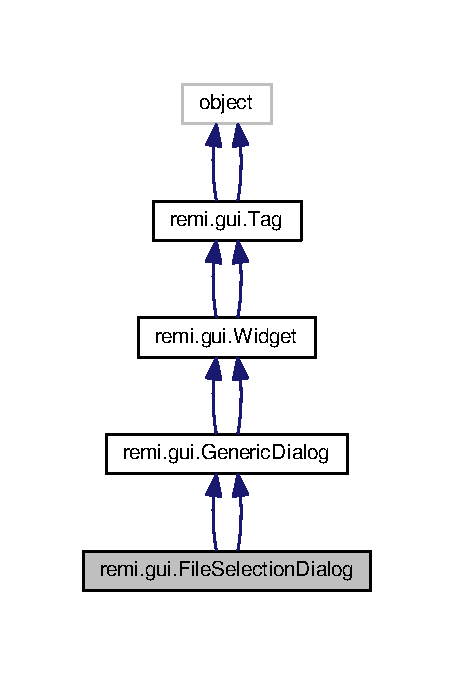
\includegraphics[width=218pt]{db/d3f/classremi_1_1gui_1_1FileSelectionDialog__inherit__graph}
\end{center}
\end{figure}


Collaboration diagram for remi.\+gui.\+File\+Selection\+Dialog\+:
\nopagebreak
\begin{figure}[H]
\begin{center}
\leavevmode
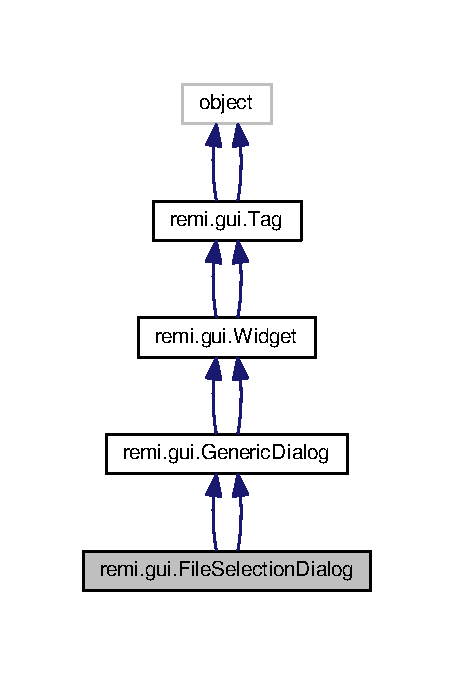
\includegraphics[width=218pt]{db/d45/classremi_1_1gui_1_1FileSelectionDialog__coll__graph}
\end{center}
\end{figure}
\subsection*{Public Member Functions}
\begin{DoxyCompactItemize}
\item 
def \hyperlink{classremi_1_1gui_1_1FileSelectionDialog_a0587b1cc5d2e2b1d300d98cb94206a50}{\+\_\+\+\_\+init\+\_\+\+\_\+} (self, title=\textquotesingle{}File dialog\textquotesingle{}, message=\textquotesingle{}Select files and folders\textquotesingle{}, multiple\+\_\+selection=True, selection\+\_\+folder=\textquotesingle{}.\textquotesingle{}, allow\+\_\+file\+\_\+selection=True, allow\+\_\+folder\+\_\+selection=True, kwargs)
\item 
def \hyperlink{classremi_1_1gui_1_1FileSelectionDialog_a23dd582a965317b649046e5e6a765a1a}{confirm\+\_\+value} (self, widget)
\item 
def \hyperlink{classremi_1_1gui_1_1FileSelectionDialog_a8e0b7dfeb324cc7c3174394543b6cf8b}{set\+\_\+on\+\_\+confirm\+\_\+value\+\_\+listener} (self, callback, userdata)
\item 
def \hyperlink{classremi_1_1gui_1_1FileSelectionDialog_a0587b1cc5d2e2b1d300d98cb94206a50}{\+\_\+\+\_\+init\+\_\+\+\_\+} (self, title=\textquotesingle{}File dialog\textquotesingle{}, message=\textquotesingle{}Select files and folders\textquotesingle{}, multiple\+\_\+selection=True, selection\+\_\+folder=\textquotesingle{}.\textquotesingle{}, allow\+\_\+file\+\_\+selection=True, allow\+\_\+folder\+\_\+selection=True, kwargs)
\item 
def \hyperlink{classremi_1_1gui_1_1FileSelectionDialog_a23dd582a965317b649046e5e6a765a1a}{confirm\+\_\+value} (self, widget)
\item 
def \hyperlink{classremi_1_1gui_1_1FileSelectionDialog_a8e0b7dfeb324cc7c3174394543b6cf8b}{set\+\_\+on\+\_\+confirm\+\_\+value\+\_\+listener} (self, callback, userdata)
\end{DoxyCompactItemize}
\subsection*{Public Attributes}
\begin{DoxyCompactItemize}
\item 
{\bfseries file\+Folder\+Navigator}\hypertarget{classremi_1_1gui_1_1FileSelectionDialog_aca750c81b8e0460e983400502ec57a1b}{}\label{classremi_1_1gui_1_1FileSelectionDialog_aca750c81b8e0460e983400502ec57a1b}

\end{DoxyCompactItemize}
\subsection*{Static Public Attributes}
\begin{DoxyCompactItemize}
\item 
string {\bfseries E\+V\+E\+N\+T\+\_\+\+O\+N\+C\+O\+N\+F\+I\+R\+M\+V\+A\+L\+UE} = \textquotesingle{}\hyperlink{classremi_1_1gui_1_1FileSelectionDialog_a23dd582a965317b649046e5e6a765a1a}{confirm\+\_\+value}\textquotesingle{}\hypertarget{classremi_1_1gui_1_1FileSelectionDialog_a2bae90f12d62adda26d53eafecb9908f}{}\label{classremi_1_1gui_1_1FileSelectionDialog_a2bae90f12d62adda26d53eafecb9908f}

\end{DoxyCompactItemize}


\subsection{Detailed Description}
\begin{DoxyVerb}file selection dialog, it opens a new webpage allows the OK/CANCEL functionality
implementing the "confirm_value" and "cancel_dialog" events.\end{DoxyVerb}
 

\subsection{Constructor \& Destructor Documentation}
\index{remi\+::gui\+::\+File\+Selection\+Dialog@{remi\+::gui\+::\+File\+Selection\+Dialog}!\+\_\+\+\_\+init\+\_\+\+\_\+@{\+\_\+\+\_\+init\+\_\+\+\_\+}}
\index{\+\_\+\+\_\+init\+\_\+\+\_\+@{\+\_\+\+\_\+init\+\_\+\+\_\+}!remi\+::gui\+::\+File\+Selection\+Dialog@{remi\+::gui\+::\+File\+Selection\+Dialog}}
\subsubsection[{\texorpdfstring{\+\_\+\+\_\+init\+\_\+\+\_\+(self, title=\textquotesingle{}\+File dialog\textquotesingle{}, message=\textquotesingle{}\+Select files and folders\textquotesingle{}, multiple\+\_\+selection=\+True, selection\+\_\+folder=\textquotesingle{}.\textquotesingle{}, allow\+\_\+file\+\_\+selection=\+True, allow\+\_\+folder\+\_\+selection=\+True, kwargs)}{__init__(self, title='File dialog', message='Select files and folders', multiple_selection=True, selection_folder='.', allow_file_selection=True, allow_folder_selection=True, kwargs)}}]{\setlength{\rightskip}{0pt plus 5cm}def remi.\+gui.\+File\+Selection\+Dialog.\+\_\+\+\_\+init\+\_\+\+\_\+ (
\begin{DoxyParamCaption}
\item[{}]{self, }
\item[{}]{title = {\ttfamily \textquotesingle{}File~dialog\textquotesingle{}}, }
\item[{}]{message = {\ttfamily \textquotesingle{}Select~files~and~folders\textquotesingle{}}, }
\item[{}]{multiple\+\_\+selection = {\ttfamily True}, }
\item[{}]{selection\+\_\+folder = {\ttfamily \textquotesingle{}.\textquotesingle{}}, }
\item[{}]{allow\+\_\+file\+\_\+selection = {\ttfamily True}, }
\item[{}]{allow\+\_\+folder\+\_\+selection = {\ttfamily True}, }
\item[{}]{kwargs}
\end{DoxyParamCaption}
)}\hypertarget{classremi_1_1gui_1_1FileSelectionDialog_a0587b1cc5d2e2b1d300d98cb94206a50}{}\label{classremi_1_1gui_1_1FileSelectionDialog_a0587b1cc5d2e2b1d300d98cb94206a50}
\begin{DoxyVerb}Args:
    title:
    message:
    multiple_selection:
    selection_folder:
    allow_file_selection:
    allow_folder_selection:
    kwargs:
\end{DoxyVerb}
 \index{remi\+::gui\+::\+File\+Selection\+Dialog@{remi\+::gui\+::\+File\+Selection\+Dialog}!\+\_\+\+\_\+init\+\_\+\+\_\+@{\+\_\+\+\_\+init\+\_\+\+\_\+}}
\index{\+\_\+\+\_\+init\+\_\+\+\_\+@{\+\_\+\+\_\+init\+\_\+\+\_\+}!remi\+::gui\+::\+File\+Selection\+Dialog@{remi\+::gui\+::\+File\+Selection\+Dialog}}
\subsubsection[{\texorpdfstring{\+\_\+\+\_\+init\+\_\+\+\_\+(self, title=\textquotesingle{}\+File dialog\textquotesingle{}, message=\textquotesingle{}\+Select files and folders\textquotesingle{}, multiple\+\_\+selection=\+True, selection\+\_\+folder=\textquotesingle{}.\textquotesingle{}, allow\+\_\+file\+\_\+selection=\+True, allow\+\_\+folder\+\_\+selection=\+True, kwargs)}{__init__(self, title='File dialog', message='Select files and folders', multiple_selection=True, selection_folder='.', allow_file_selection=True, allow_folder_selection=True, kwargs)}}]{\setlength{\rightskip}{0pt plus 5cm}def remi.\+gui.\+File\+Selection\+Dialog.\+\_\+\+\_\+init\+\_\+\+\_\+ (
\begin{DoxyParamCaption}
\item[{}]{self, }
\item[{}]{title = {\ttfamily \textquotesingle{}File~dialog\textquotesingle{}}, }
\item[{}]{message = {\ttfamily \textquotesingle{}Select~files~and~folders\textquotesingle{}}, }
\item[{}]{multiple\+\_\+selection = {\ttfamily True}, }
\item[{}]{selection\+\_\+folder = {\ttfamily \textquotesingle{}.\textquotesingle{}}, }
\item[{}]{allow\+\_\+file\+\_\+selection = {\ttfamily True}, }
\item[{}]{allow\+\_\+folder\+\_\+selection = {\ttfamily True}, }
\item[{}]{kwargs}
\end{DoxyParamCaption}
)}\hypertarget{classremi_1_1gui_1_1FileSelectionDialog_a0587b1cc5d2e2b1d300d98cb94206a50}{}\label{classremi_1_1gui_1_1FileSelectionDialog_a0587b1cc5d2e2b1d300d98cb94206a50}
\begin{DoxyVerb}Args:
    title:
    message:
    multiple_selection:
    selection_folder:
    allow_file_selection:
    allow_folder_selection:
    kwargs:
\end{DoxyVerb}
 

\subsection{Member Function Documentation}
\index{remi\+::gui\+::\+File\+Selection\+Dialog@{remi\+::gui\+::\+File\+Selection\+Dialog}!confirm\+\_\+value@{confirm\+\_\+value}}
\index{confirm\+\_\+value@{confirm\+\_\+value}!remi\+::gui\+::\+File\+Selection\+Dialog@{remi\+::gui\+::\+File\+Selection\+Dialog}}
\subsubsection[{\texorpdfstring{confirm\+\_\+value(self, widget)}{confirm_value(self, widget)}}]{\setlength{\rightskip}{0pt plus 5cm}def remi.\+gui.\+File\+Selection\+Dialog.\+confirm\+\_\+value (
\begin{DoxyParamCaption}
\item[{}]{self, }
\item[{}]{widget}
\end{DoxyParamCaption}
)}\hypertarget{classremi_1_1gui_1_1FileSelectionDialog_a23dd582a965317b649046e5e6a765a1a}{}\label{classremi_1_1gui_1_1FileSelectionDialog_a23dd582a965317b649046e5e6a765a1a}
\begin{DoxyVerb}event called pressing on OK button.
   propagates the string content of the input field
\end{DoxyVerb}
 \index{remi\+::gui\+::\+File\+Selection\+Dialog@{remi\+::gui\+::\+File\+Selection\+Dialog}!confirm\+\_\+value@{confirm\+\_\+value}}
\index{confirm\+\_\+value@{confirm\+\_\+value}!remi\+::gui\+::\+File\+Selection\+Dialog@{remi\+::gui\+::\+File\+Selection\+Dialog}}
\subsubsection[{\texorpdfstring{confirm\+\_\+value(self, widget)}{confirm_value(self, widget)}}]{\setlength{\rightskip}{0pt plus 5cm}def remi.\+gui.\+File\+Selection\+Dialog.\+confirm\+\_\+value (
\begin{DoxyParamCaption}
\item[{}]{self, }
\item[{}]{widget}
\end{DoxyParamCaption}
)}\hypertarget{classremi_1_1gui_1_1FileSelectionDialog_a23dd582a965317b649046e5e6a765a1a}{}\label{classremi_1_1gui_1_1FileSelectionDialog_a23dd582a965317b649046e5e6a765a1a}
\begin{DoxyVerb}event called pressing on OK button.
   propagates the string content of the input field
\end{DoxyVerb}
 \index{remi\+::gui\+::\+File\+Selection\+Dialog@{remi\+::gui\+::\+File\+Selection\+Dialog}!set\+\_\+on\+\_\+confirm\+\_\+value\+\_\+listener@{set\+\_\+on\+\_\+confirm\+\_\+value\+\_\+listener}}
\index{set\+\_\+on\+\_\+confirm\+\_\+value\+\_\+listener@{set\+\_\+on\+\_\+confirm\+\_\+value\+\_\+listener}!remi\+::gui\+::\+File\+Selection\+Dialog@{remi\+::gui\+::\+File\+Selection\+Dialog}}
\subsubsection[{\texorpdfstring{set\+\_\+on\+\_\+confirm\+\_\+value\+\_\+listener(self, callback, userdata)}{set_on_confirm_value_listener(self, callback, userdata)}}]{\setlength{\rightskip}{0pt plus 5cm}def remi.\+gui.\+File\+Selection\+Dialog.\+set\+\_\+on\+\_\+confirm\+\_\+value\+\_\+listener (
\begin{DoxyParamCaption}
\item[{}]{self, }
\item[{}]{callback, }
\item[{}]{userdata}
\end{DoxyParamCaption}
)}\hypertarget{classremi_1_1gui_1_1FileSelectionDialog_a8e0b7dfeb324cc7c3174394543b6cf8b}{}\label{classremi_1_1gui_1_1FileSelectionDialog_a8e0b7dfeb324cc7c3174394543b6cf8b}
\begin{DoxyVerb}Register the listener for the on_confirm event.

Note: the listener prototype have to be in the form
on_file_selection_confirm(self, widget, selectedFileStringList).
\end{DoxyVerb}
 \index{remi\+::gui\+::\+File\+Selection\+Dialog@{remi\+::gui\+::\+File\+Selection\+Dialog}!set\+\_\+on\+\_\+confirm\+\_\+value\+\_\+listener@{set\+\_\+on\+\_\+confirm\+\_\+value\+\_\+listener}}
\index{set\+\_\+on\+\_\+confirm\+\_\+value\+\_\+listener@{set\+\_\+on\+\_\+confirm\+\_\+value\+\_\+listener}!remi\+::gui\+::\+File\+Selection\+Dialog@{remi\+::gui\+::\+File\+Selection\+Dialog}}
\subsubsection[{\texorpdfstring{set\+\_\+on\+\_\+confirm\+\_\+value\+\_\+listener(self, callback, userdata)}{set_on_confirm_value_listener(self, callback, userdata)}}]{\setlength{\rightskip}{0pt plus 5cm}def remi.\+gui.\+File\+Selection\+Dialog.\+set\+\_\+on\+\_\+confirm\+\_\+value\+\_\+listener (
\begin{DoxyParamCaption}
\item[{}]{self, }
\item[{}]{callback, }
\item[{}]{userdata}
\end{DoxyParamCaption}
)}\hypertarget{classremi_1_1gui_1_1FileSelectionDialog_a8e0b7dfeb324cc7c3174394543b6cf8b}{}\label{classremi_1_1gui_1_1FileSelectionDialog_a8e0b7dfeb324cc7c3174394543b6cf8b}
\begin{DoxyVerb}Register the listener for the on_confirm event.

Note: the listener prototype have to be in the form
on_file_selection_confirm(self, widget, selectedFileStringList).
\end{DoxyVerb}
 

The documentation for this class was generated from the following file\+:\begin{DoxyCompactItemize}
\item 
Compiled/\+Server/remi/gui.\+py\end{DoxyCompactItemize}

\hypertarget{classremi_1_1gui_1_1FileUploader}{}\section{remi.\+gui.\+File\+Uploader Class Reference}
\label{classremi_1_1gui_1_1FileUploader}\index{remi.\+gui.\+File\+Uploader@{remi.\+gui.\+File\+Uploader}}


Inheritance diagram for remi.\+gui.\+File\+Uploader\+:
\nopagebreak
\begin{figure}[H]
\begin{center}
\leavevmode
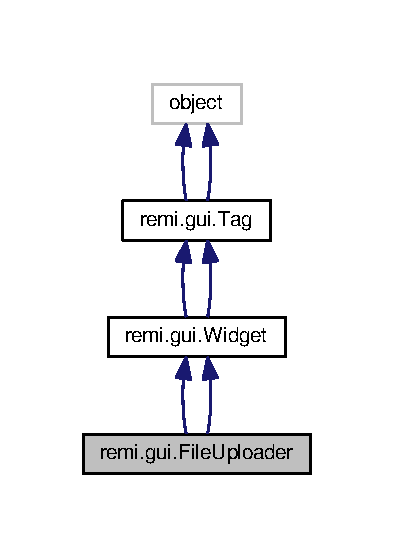
\includegraphics[width=189pt]{d5/daa/classremi_1_1gui_1_1FileUploader__inherit__graph}
\end{center}
\end{figure}


Collaboration diagram for remi.\+gui.\+File\+Uploader\+:
\nopagebreak
\begin{figure}[H]
\begin{center}
\leavevmode
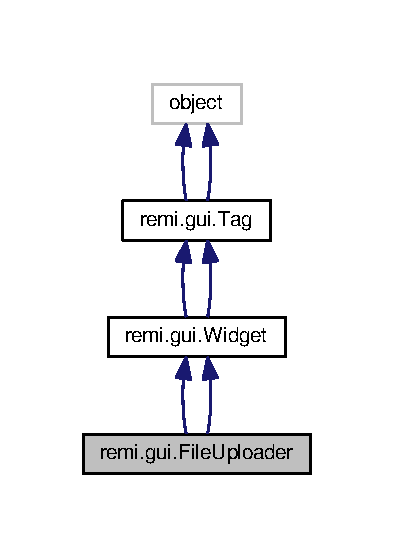
\includegraphics[width=189pt]{d8/df7/classremi_1_1gui_1_1FileUploader__coll__graph}
\end{center}
\end{figure}
\subsection*{Public Member Functions}
\begin{DoxyCompactItemize}
\item 
def \hyperlink{classremi_1_1gui_1_1FileUploader_aecabe8b6d84e2cf14703d88ba3736633}{\+\_\+\+\_\+init\+\_\+\+\_\+} (self, savepath=\textquotesingle{}./\textquotesingle{}, multiple\+\_\+selection\+\_\+allowed=False, kwargs)
\item 
def \hyperlink{classremi_1_1gui_1_1FileUploader_aad3d08bc689526321294786dd09613cf}{onsuccess} (self, filename)
\item 
def \hyperlink{classremi_1_1gui_1_1FileUploader_a0855160a9b0f52ff31aa7d6561f32038}{set\+\_\+on\+\_\+success\+\_\+listener} (self, callback, userdata)
\item 
def \hyperlink{classremi_1_1gui_1_1FileUploader_ade6a041ea0bcc7608c559cd860c32eea}{onfailed} (self, filename)
\item 
def \hyperlink{classremi_1_1gui_1_1FileUploader_a6fb7795ee0173250c2788975e6bcf5ed}{set\+\_\+on\+\_\+failed\+\_\+listener} (self, callback, userdata)
\item 
def \hyperlink{classremi_1_1gui_1_1FileUploader_a2c3e86dd58017e56d87323b4f738439e}{ondata} (self, filedata, filename)
\item 
def \hyperlink{classremi_1_1gui_1_1FileUploader_a7dfc6cb9332ac30f340fd1aad6dcc647}{set\+\_\+on\+\_\+data\+\_\+listener} (self, callback, userdata)
\item 
def \hyperlink{classremi_1_1gui_1_1FileUploader_aecabe8b6d84e2cf14703d88ba3736633}{\+\_\+\+\_\+init\+\_\+\+\_\+} (self, savepath=\textquotesingle{}./\textquotesingle{}, multiple\+\_\+selection\+\_\+allowed=False, kwargs)
\item 
def \hyperlink{classremi_1_1gui_1_1FileUploader_aad3d08bc689526321294786dd09613cf}{onsuccess} (self, filename)
\item 
def \hyperlink{classremi_1_1gui_1_1FileUploader_a0855160a9b0f52ff31aa7d6561f32038}{set\+\_\+on\+\_\+success\+\_\+listener} (self, callback, userdata)
\item 
def \hyperlink{classremi_1_1gui_1_1FileUploader_ade6a041ea0bcc7608c559cd860c32eea}{onfailed} (self, filename)
\item 
def \hyperlink{classremi_1_1gui_1_1FileUploader_a6fb7795ee0173250c2788975e6bcf5ed}{set\+\_\+on\+\_\+failed\+\_\+listener} (self, callback, userdata)
\item 
def \hyperlink{classremi_1_1gui_1_1FileUploader_a2c3e86dd58017e56d87323b4f738439e}{ondata} (self, filedata, filename)
\item 
def \hyperlink{classremi_1_1gui_1_1FileUploader_a7dfc6cb9332ac30f340fd1aad6dcc647}{set\+\_\+on\+\_\+data\+\_\+listener} (self, callback, userdata)
\end{DoxyCompactItemize}
\subsection*{Public Attributes}
\begin{DoxyCompactItemize}
\item 
{\bfseries type}\hypertarget{classremi_1_1gui_1_1FileUploader_ae7daaa670f80c08b326d3a95847b1bde}{}\label{classremi_1_1gui_1_1FileUploader_ae7daaa670f80c08b326d3a95847b1bde}

\item 
{\bfseries E\+V\+E\+N\+T\+\_\+\+O\+N\+\_\+\+S\+U\+C\+C\+E\+SS}\hypertarget{classremi_1_1gui_1_1FileUploader_acd673d8b6336fd75e0a03078b06a5106}{}\label{classremi_1_1gui_1_1FileUploader_acd673d8b6336fd75e0a03078b06a5106}

\item 
{\bfseries E\+V\+E\+N\+T\+\_\+\+O\+N\+\_\+\+F\+A\+I\+L\+ED}\hypertarget{classremi_1_1gui_1_1FileUploader_a4dbc1939726417fe5a958f3ee851cc5f}{}\label{classremi_1_1gui_1_1FileUploader_a4dbc1939726417fe5a958f3ee851cc5f}

\item 
{\bfseries E\+V\+E\+N\+T\+\_\+\+O\+N\+\_\+\+D\+A\+TA}\hypertarget{classremi_1_1gui_1_1FileUploader_a41e688e9604be2bea5b895473d3d664f}{}\label{classremi_1_1gui_1_1FileUploader_a41e688e9604be2bea5b895473d3d664f}

\end{DoxyCompactItemize}
\subsection*{Additional Inherited Members}


\subsection{Detailed Description}
\begin{DoxyVerb}FileUploader widget:
    allows to upload multiple files to a specified folder.
    implements the onsuccess and onfailed events.
\end{DoxyVerb}
 

\subsection{Constructor \& Destructor Documentation}
\index{remi\+::gui\+::\+File\+Uploader@{remi\+::gui\+::\+File\+Uploader}!\+\_\+\+\_\+init\+\_\+\+\_\+@{\+\_\+\+\_\+init\+\_\+\+\_\+}}
\index{\+\_\+\+\_\+init\+\_\+\+\_\+@{\+\_\+\+\_\+init\+\_\+\+\_\+}!remi\+::gui\+::\+File\+Uploader@{remi\+::gui\+::\+File\+Uploader}}
\subsubsection[{\texorpdfstring{\+\_\+\+\_\+init\+\_\+\+\_\+(self, savepath=\textquotesingle{}./\textquotesingle{}, multiple\+\_\+selection\+\_\+allowed=\+False, kwargs)}{__init__(self, savepath='./', multiple_selection_allowed=False, kwargs)}}]{\setlength{\rightskip}{0pt plus 5cm}def remi.\+gui.\+File\+Uploader.\+\_\+\+\_\+init\+\_\+\+\_\+ (
\begin{DoxyParamCaption}
\item[{}]{self, }
\item[{}]{savepath = {\ttfamily \textquotesingle{}./\textquotesingle{}}, }
\item[{}]{multiple\+\_\+selection\+\_\+allowed = {\ttfamily False}, }
\item[{}]{kwargs}
\end{DoxyParamCaption}
)}\hypertarget{classremi_1_1gui_1_1FileUploader_aecabe8b6d84e2cf14703d88ba3736633}{}\label{classremi_1_1gui_1_1FileUploader_aecabe8b6d84e2cf14703d88ba3736633}
\begin{DoxyVerb}Args:
    savepath:
    multiple_selection_allowed:
    kwargs:
\end{DoxyVerb}
 \index{remi\+::gui\+::\+File\+Uploader@{remi\+::gui\+::\+File\+Uploader}!\+\_\+\+\_\+init\+\_\+\+\_\+@{\+\_\+\+\_\+init\+\_\+\+\_\+}}
\index{\+\_\+\+\_\+init\+\_\+\+\_\+@{\+\_\+\+\_\+init\+\_\+\+\_\+}!remi\+::gui\+::\+File\+Uploader@{remi\+::gui\+::\+File\+Uploader}}
\subsubsection[{\texorpdfstring{\+\_\+\+\_\+init\+\_\+\+\_\+(self, savepath=\textquotesingle{}./\textquotesingle{}, multiple\+\_\+selection\+\_\+allowed=\+False, kwargs)}{__init__(self, savepath='./', multiple_selection_allowed=False, kwargs)}}]{\setlength{\rightskip}{0pt plus 5cm}def remi.\+gui.\+File\+Uploader.\+\_\+\+\_\+init\+\_\+\+\_\+ (
\begin{DoxyParamCaption}
\item[{}]{self, }
\item[{}]{savepath = {\ttfamily \textquotesingle{}./\textquotesingle{}}, }
\item[{}]{multiple\+\_\+selection\+\_\+allowed = {\ttfamily False}, }
\item[{}]{kwargs}
\end{DoxyParamCaption}
)}\hypertarget{classremi_1_1gui_1_1FileUploader_aecabe8b6d84e2cf14703d88ba3736633}{}\label{classremi_1_1gui_1_1FileUploader_aecabe8b6d84e2cf14703d88ba3736633}
\begin{DoxyVerb}Args:
    savepath:
    multiple_selection_allowed:
    kwargs:
\end{DoxyVerb}
 

\subsection{Member Function Documentation}
\index{remi\+::gui\+::\+File\+Uploader@{remi\+::gui\+::\+File\+Uploader}!ondata@{ondata}}
\index{ondata@{ondata}!remi\+::gui\+::\+File\+Uploader@{remi\+::gui\+::\+File\+Uploader}}
\subsubsection[{\texorpdfstring{ondata(self, filedata, filename)}{ondata(self, filedata, filename)}}]{\setlength{\rightskip}{0pt plus 5cm}def remi.\+gui.\+File\+Uploader.\+ondata (
\begin{DoxyParamCaption}
\item[{}]{self, }
\item[{}]{filedata, }
\item[{}]{filename}
\end{DoxyParamCaption}
)}\hypertarget{classremi_1_1gui_1_1FileUploader_a2c3e86dd58017e56d87323b4f738439e}{}\label{classremi_1_1gui_1_1FileUploader_a2c3e86dd58017e56d87323b4f738439e}
\begin{DoxyVerb}Args:
    filedata:
    filename:

Returns:\end{DoxyVerb}
 \index{remi\+::gui\+::\+File\+Uploader@{remi\+::gui\+::\+File\+Uploader}!ondata@{ondata}}
\index{ondata@{ondata}!remi\+::gui\+::\+File\+Uploader@{remi\+::gui\+::\+File\+Uploader}}
\subsubsection[{\texorpdfstring{ondata(self, filedata, filename)}{ondata(self, filedata, filename)}}]{\setlength{\rightskip}{0pt plus 5cm}def remi.\+gui.\+File\+Uploader.\+ondata (
\begin{DoxyParamCaption}
\item[{}]{self, }
\item[{}]{filedata, }
\item[{}]{filename}
\end{DoxyParamCaption}
)}\hypertarget{classremi_1_1gui_1_1FileUploader_a2c3e86dd58017e56d87323b4f738439e}{}\label{classremi_1_1gui_1_1FileUploader_a2c3e86dd58017e56d87323b4f738439e}
\begin{DoxyVerb}Args:
    filedata:
    filename:

Returns:\end{DoxyVerb}
 \index{remi\+::gui\+::\+File\+Uploader@{remi\+::gui\+::\+File\+Uploader}!onfailed@{onfailed}}
\index{onfailed@{onfailed}!remi\+::gui\+::\+File\+Uploader@{remi\+::gui\+::\+File\+Uploader}}
\subsubsection[{\texorpdfstring{onfailed(self, filename)}{onfailed(self, filename)}}]{\setlength{\rightskip}{0pt plus 5cm}def remi.\+gui.\+File\+Uploader.\+onfailed (
\begin{DoxyParamCaption}
\item[{}]{self, }
\item[{}]{filename}
\end{DoxyParamCaption}
)}\hypertarget{classremi_1_1gui_1_1FileUploader_ade6a041ea0bcc7608c559cd860c32eea}{}\label{classremi_1_1gui_1_1FileUploader_ade6a041ea0bcc7608c559cd860c32eea}
\begin{DoxyVerb}Args:
    filename:

Returns:\end{DoxyVerb}
 \index{remi\+::gui\+::\+File\+Uploader@{remi\+::gui\+::\+File\+Uploader}!onfailed@{onfailed}}
\index{onfailed@{onfailed}!remi\+::gui\+::\+File\+Uploader@{remi\+::gui\+::\+File\+Uploader}}
\subsubsection[{\texorpdfstring{onfailed(self, filename)}{onfailed(self, filename)}}]{\setlength{\rightskip}{0pt plus 5cm}def remi.\+gui.\+File\+Uploader.\+onfailed (
\begin{DoxyParamCaption}
\item[{}]{self, }
\item[{}]{filename}
\end{DoxyParamCaption}
)}\hypertarget{classremi_1_1gui_1_1FileUploader_ade6a041ea0bcc7608c559cd860c32eea}{}\label{classremi_1_1gui_1_1FileUploader_ade6a041ea0bcc7608c559cd860c32eea}
\begin{DoxyVerb}Args:
    filename:

Returns:\end{DoxyVerb}
 \index{remi\+::gui\+::\+File\+Uploader@{remi\+::gui\+::\+File\+Uploader}!onsuccess@{onsuccess}}
\index{onsuccess@{onsuccess}!remi\+::gui\+::\+File\+Uploader@{remi\+::gui\+::\+File\+Uploader}}
\subsubsection[{\texorpdfstring{onsuccess(self, filename)}{onsuccess(self, filename)}}]{\setlength{\rightskip}{0pt plus 5cm}def remi.\+gui.\+File\+Uploader.\+onsuccess (
\begin{DoxyParamCaption}
\item[{}]{self, }
\item[{}]{filename}
\end{DoxyParamCaption}
)}\hypertarget{classremi_1_1gui_1_1FileUploader_aad3d08bc689526321294786dd09613cf}{}\label{classremi_1_1gui_1_1FileUploader_aad3d08bc689526321294786dd09613cf}
\begin{DoxyVerb}Args:
    filename:

Returns:\end{DoxyVerb}
 \index{remi\+::gui\+::\+File\+Uploader@{remi\+::gui\+::\+File\+Uploader}!onsuccess@{onsuccess}}
\index{onsuccess@{onsuccess}!remi\+::gui\+::\+File\+Uploader@{remi\+::gui\+::\+File\+Uploader}}
\subsubsection[{\texorpdfstring{onsuccess(self, filename)}{onsuccess(self, filename)}}]{\setlength{\rightskip}{0pt plus 5cm}def remi.\+gui.\+File\+Uploader.\+onsuccess (
\begin{DoxyParamCaption}
\item[{}]{self, }
\item[{}]{filename}
\end{DoxyParamCaption}
)}\hypertarget{classremi_1_1gui_1_1FileUploader_aad3d08bc689526321294786dd09613cf}{}\label{classremi_1_1gui_1_1FileUploader_aad3d08bc689526321294786dd09613cf}
\begin{DoxyVerb}Args:
    filename:

Returns:\end{DoxyVerb}
 \index{remi\+::gui\+::\+File\+Uploader@{remi\+::gui\+::\+File\+Uploader}!set\+\_\+on\+\_\+data\+\_\+listener@{set\+\_\+on\+\_\+data\+\_\+listener}}
\index{set\+\_\+on\+\_\+data\+\_\+listener@{set\+\_\+on\+\_\+data\+\_\+listener}!remi\+::gui\+::\+File\+Uploader@{remi\+::gui\+::\+File\+Uploader}}
\subsubsection[{\texorpdfstring{set\+\_\+on\+\_\+data\+\_\+listener(self, callback, userdata)}{set_on_data_listener(self, callback, userdata)}}]{\setlength{\rightskip}{0pt plus 5cm}def remi.\+gui.\+File\+Uploader.\+set\+\_\+on\+\_\+data\+\_\+listener (
\begin{DoxyParamCaption}
\item[{}]{self, }
\item[{}]{callback, }
\item[{}]{userdata}
\end{DoxyParamCaption}
)}\hypertarget{classremi_1_1gui_1_1FileUploader_a7dfc6cb9332ac30f340fd1aad6dcc647}{}\label{classremi_1_1gui_1_1FileUploader_a7dfc6cb9332ac30f340fd1aad6dcc647}
\begin{DoxyVerb}Register the listener for the ondata event.

Note: the listener prototype have to be in the form on_fileupload_data(self, widget, filedata, filename),
    where filedata is the bytearray chunk.
\end{DoxyVerb}
 \index{remi\+::gui\+::\+File\+Uploader@{remi\+::gui\+::\+File\+Uploader}!set\+\_\+on\+\_\+data\+\_\+listener@{set\+\_\+on\+\_\+data\+\_\+listener}}
\index{set\+\_\+on\+\_\+data\+\_\+listener@{set\+\_\+on\+\_\+data\+\_\+listener}!remi\+::gui\+::\+File\+Uploader@{remi\+::gui\+::\+File\+Uploader}}
\subsubsection[{\texorpdfstring{set\+\_\+on\+\_\+data\+\_\+listener(self, callback, userdata)}{set_on_data_listener(self, callback, userdata)}}]{\setlength{\rightskip}{0pt plus 5cm}def remi.\+gui.\+File\+Uploader.\+set\+\_\+on\+\_\+data\+\_\+listener (
\begin{DoxyParamCaption}
\item[{}]{self, }
\item[{}]{callback, }
\item[{}]{userdata}
\end{DoxyParamCaption}
)}\hypertarget{classremi_1_1gui_1_1FileUploader_a7dfc6cb9332ac30f340fd1aad6dcc647}{}\label{classremi_1_1gui_1_1FileUploader_a7dfc6cb9332ac30f340fd1aad6dcc647}
\begin{DoxyVerb}Register the listener for the ondata event.

Note: the listener prototype have to be in the form on_fileupload_data(self, widget, filedata, filename),
    where filedata is the bytearray chunk.
\end{DoxyVerb}
 \index{remi\+::gui\+::\+File\+Uploader@{remi\+::gui\+::\+File\+Uploader}!set\+\_\+on\+\_\+failed\+\_\+listener@{set\+\_\+on\+\_\+failed\+\_\+listener}}
\index{set\+\_\+on\+\_\+failed\+\_\+listener@{set\+\_\+on\+\_\+failed\+\_\+listener}!remi\+::gui\+::\+File\+Uploader@{remi\+::gui\+::\+File\+Uploader}}
\subsubsection[{\texorpdfstring{set\+\_\+on\+\_\+failed\+\_\+listener(self, callback, userdata)}{set_on_failed_listener(self, callback, userdata)}}]{\setlength{\rightskip}{0pt plus 5cm}def remi.\+gui.\+File\+Uploader.\+set\+\_\+on\+\_\+failed\+\_\+listener (
\begin{DoxyParamCaption}
\item[{}]{self, }
\item[{}]{callback, }
\item[{}]{userdata}
\end{DoxyParamCaption}
)}\hypertarget{classremi_1_1gui_1_1FileUploader_a6fb7795ee0173250c2788975e6bcf5ed}{}\label{classremi_1_1gui_1_1FileUploader_a6fb7795ee0173250c2788975e6bcf5ed}
\begin{DoxyVerb}Register the listener for the onfailed event.

Note: the listener prototype have to be in the form on_fileupload_failed(self, widget, filename).
\end{DoxyVerb}
 \index{remi\+::gui\+::\+File\+Uploader@{remi\+::gui\+::\+File\+Uploader}!set\+\_\+on\+\_\+failed\+\_\+listener@{set\+\_\+on\+\_\+failed\+\_\+listener}}
\index{set\+\_\+on\+\_\+failed\+\_\+listener@{set\+\_\+on\+\_\+failed\+\_\+listener}!remi\+::gui\+::\+File\+Uploader@{remi\+::gui\+::\+File\+Uploader}}
\subsubsection[{\texorpdfstring{set\+\_\+on\+\_\+failed\+\_\+listener(self, callback, userdata)}{set_on_failed_listener(self, callback, userdata)}}]{\setlength{\rightskip}{0pt plus 5cm}def remi.\+gui.\+File\+Uploader.\+set\+\_\+on\+\_\+failed\+\_\+listener (
\begin{DoxyParamCaption}
\item[{}]{self, }
\item[{}]{callback, }
\item[{}]{userdata}
\end{DoxyParamCaption}
)}\hypertarget{classremi_1_1gui_1_1FileUploader_a6fb7795ee0173250c2788975e6bcf5ed}{}\label{classremi_1_1gui_1_1FileUploader_a6fb7795ee0173250c2788975e6bcf5ed}
\begin{DoxyVerb}Register the listener for the onfailed event.

Note: the listener prototype have to be in the form on_fileupload_failed(self, widget, filename).
\end{DoxyVerb}
 \index{remi\+::gui\+::\+File\+Uploader@{remi\+::gui\+::\+File\+Uploader}!set\+\_\+on\+\_\+success\+\_\+listener@{set\+\_\+on\+\_\+success\+\_\+listener}}
\index{set\+\_\+on\+\_\+success\+\_\+listener@{set\+\_\+on\+\_\+success\+\_\+listener}!remi\+::gui\+::\+File\+Uploader@{remi\+::gui\+::\+File\+Uploader}}
\subsubsection[{\texorpdfstring{set\+\_\+on\+\_\+success\+\_\+listener(self, callback, userdata)}{set_on_success_listener(self, callback, userdata)}}]{\setlength{\rightskip}{0pt plus 5cm}def remi.\+gui.\+File\+Uploader.\+set\+\_\+on\+\_\+success\+\_\+listener (
\begin{DoxyParamCaption}
\item[{}]{self, }
\item[{}]{callback, }
\item[{}]{userdata}
\end{DoxyParamCaption}
)}\hypertarget{classremi_1_1gui_1_1FileUploader_a0855160a9b0f52ff31aa7d6561f32038}{}\label{classremi_1_1gui_1_1FileUploader_a0855160a9b0f52ff31aa7d6561f32038}
\begin{DoxyVerb}Register the listener for the onsuccess event.

Note: the listener prototype have to be in the form on_fileupload_success(self, widget, filename).
\end{DoxyVerb}
 \index{remi\+::gui\+::\+File\+Uploader@{remi\+::gui\+::\+File\+Uploader}!set\+\_\+on\+\_\+success\+\_\+listener@{set\+\_\+on\+\_\+success\+\_\+listener}}
\index{set\+\_\+on\+\_\+success\+\_\+listener@{set\+\_\+on\+\_\+success\+\_\+listener}!remi\+::gui\+::\+File\+Uploader@{remi\+::gui\+::\+File\+Uploader}}
\subsubsection[{\texorpdfstring{set\+\_\+on\+\_\+success\+\_\+listener(self, callback, userdata)}{set_on_success_listener(self, callback, userdata)}}]{\setlength{\rightskip}{0pt plus 5cm}def remi.\+gui.\+File\+Uploader.\+set\+\_\+on\+\_\+success\+\_\+listener (
\begin{DoxyParamCaption}
\item[{}]{self, }
\item[{}]{callback, }
\item[{}]{userdata}
\end{DoxyParamCaption}
)}\hypertarget{classremi_1_1gui_1_1FileUploader_a0855160a9b0f52ff31aa7d6561f32038}{}\label{classremi_1_1gui_1_1FileUploader_a0855160a9b0f52ff31aa7d6561f32038}
\begin{DoxyVerb}Register the listener for the onsuccess event.

Note: the listener prototype have to be in the form on_fileupload_success(self, widget, filename).
\end{DoxyVerb}
 

The documentation for this class was generated from the following file\+:\begin{DoxyCompactItemize}
\item 
Compiled/\+Server/remi/gui.\+py\end{DoxyCompactItemize}

\hypertarget{classremi_1_1gui_1_1GenericDialog}{}\section{remi.\+gui.\+Generic\+Dialog Class Reference}
\label{classremi_1_1gui_1_1GenericDialog}\index{remi.\+gui.\+Generic\+Dialog@{remi.\+gui.\+Generic\+Dialog}}


Inheritance diagram for remi.\+gui.\+Generic\+Dialog\+:
\nopagebreak
\begin{figure}[H]
\begin{center}
\leavevmode
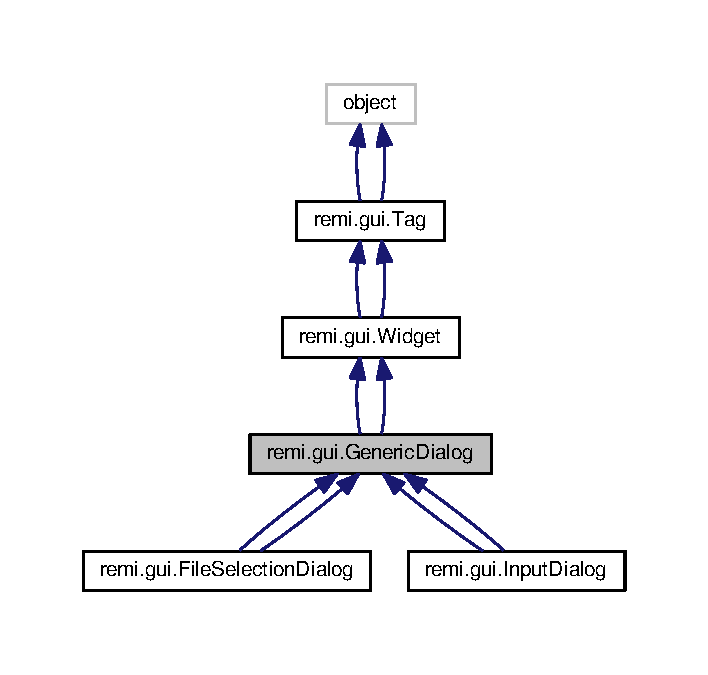
\includegraphics[width=340pt]{d6/de3/classremi_1_1gui_1_1GenericDialog__inherit__graph}
\end{center}
\end{figure}


Collaboration diagram for remi.\+gui.\+Generic\+Dialog\+:
\nopagebreak
\begin{figure}[H]
\begin{center}
\leavevmode
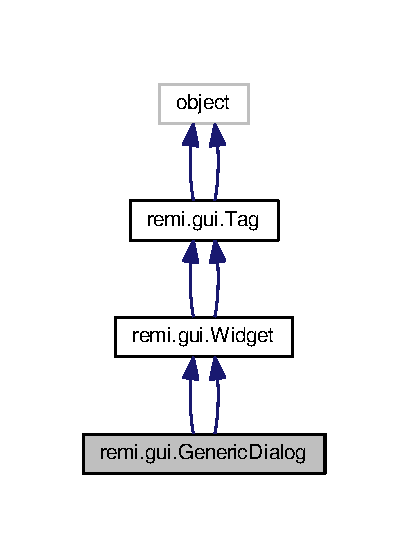
\includegraphics[width=196pt]{db/d9d/classremi_1_1gui_1_1GenericDialog__coll__graph}
\end{center}
\end{figure}
\subsection*{Public Member Functions}
\begin{DoxyCompactItemize}
\item 
def \hyperlink{classremi_1_1gui_1_1GenericDialog_a5d6eda71557518b78261e1007d0e4b4b}{\+\_\+\+\_\+init\+\_\+\+\_\+} (self, title=\textquotesingle{}\textquotesingle{}, message=\textquotesingle{}\textquotesingle{}, kwargs)
\item 
def \hyperlink{classremi_1_1gui_1_1GenericDialog_a40e873d6cdd600eb2632ab60a504fac4}{add\+\_\+field\+\_\+with\+\_\+label} (self, key, label\+\_\+description, field)
\item 
def \hyperlink{classremi_1_1gui_1_1GenericDialog_aedb713b0aa165232509b5d64b56d93b7}{add\+\_\+field} (self, key, field)
\item 
def \hyperlink{classremi_1_1gui_1_1GenericDialog_abe3376922b34089d38e2af903708dc7f}{get\+\_\+field} (self, key)
\item 
def \hyperlink{classremi_1_1gui_1_1GenericDialog_afb62d4e48291115923d9dae74841a989}{confirm\+\_\+dialog} (self)
\item 
def \hyperlink{classremi_1_1gui_1_1GenericDialog_a255f09292492e190f01c87394fce2c15}{set\+\_\+on\+\_\+confirm\+\_\+dialog\+\_\+listener} (self, callback, userdata)
\item 
def \hyperlink{classremi_1_1gui_1_1GenericDialog_a23650c8959545f1a4c50b9b375f0412d}{cancel\+\_\+dialog} (self)
\item 
def \hyperlink{classremi_1_1gui_1_1GenericDialog_ae45abbd039d70a70f5134e843a7fb91e}{set\+\_\+on\+\_\+cancel\+\_\+dialog\+\_\+listener} (self, callback, userdata)
\item 
def \hyperlink{classremi_1_1gui_1_1GenericDialog_ad7ac0adef763e683bfc87a289392bb11}{show} (self, base\+\_\+app\+\_\+instance)
\item 
def \hyperlink{classremi_1_1gui_1_1GenericDialog_ab228c4ebfd696414b4a5c04f5ec55e67}{hide} (self)
\item 
def \hyperlink{classremi_1_1gui_1_1GenericDialog_a5d6eda71557518b78261e1007d0e4b4b}{\+\_\+\+\_\+init\+\_\+\+\_\+} (self, title=\textquotesingle{}\textquotesingle{}, message=\textquotesingle{}\textquotesingle{}, kwargs)
\item 
def \hyperlink{classremi_1_1gui_1_1GenericDialog_a40e873d6cdd600eb2632ab60a504fac4}{add\+\_\+field\+\_\+with\+\_\+label} (self, key, label\+\_\+description, field)
\item 
def \hyperlink{classremi_1_1gui_1_1GenericDialog_aedb713b0aa165232509b5d64b56d93b7}{add\+\_\+field} (self, key, field)
\item 
def \hyperlink{classremi_1_1gui_1_1GenericDialog_abe3376922b34089d38e2af903708dc7f}{get\+\_\+field} (self, key)
\item 
def \hyperlink{classremi_1_1gui_1_1GenericDialog_afb62d4e48291115923d9dae74841a989}{confirm\+\_\+dialog} (self)
\item 
def \hyperlink{classremi_1_1gui_1_1GenericDialog_a255f09292492e190f01c87394fce2c15}{set\+\_\+on\+\_\+confirm\+\_\+dialog\+\_\+listener} (self, callback, userdata)
\item 
def \hyperlink{classremi_1_1gui_1_1GenericDialog_a23650c8959545f1a4c50b9b375f0412d}{cancel\+\_\+dialog} (self)
\item 
def \hyperlink{classremi_1_1gui_1_1GenericDialog_ae45abbd039d70a70f5134e843a7fb91e}{set\+\_\+on\+\_\+cancel\+\_\+dialog\+\_\+listener} (self, callback, userdata)
\item 
def \hyperlink{classremi_1_1gui_1_1GenericDialog_ad7ac0adef763e683bfc87a289392bb11}{show} (self, base\+\_\+app\+\_\+instance)
\item 
def \hyperlink{classremi_1_1gui_1_1GenericDialog_ab228c4ebfd696414b4a5c04f5ec55e67}{hide} (self)
\end{DoxyCompactItemize}
\subsection*{Public Attributes}
\begin{DoxyCompactItemize}
\item 
{\bfseries container}\hypertarget{classremi_1_1gui_1_1GenericDialog_a64988716e9f35b583d5b1a9c025b3883}{}\label{classremi_1_1gui_1_1GenericDialog_a64988716e9f35b583d5b1a9c025b3883}

\item 
{\bfseries conf}\hypertarget{classremi_1_1gui_1_1GenericDialog_a636108546940b87a6d27c6d4adbd1db9}{}\label{classremi_1_1gui_1_1GenericDialog_a636108546940b87a6d27c6d4adbd1db9}

\item 
{\bfseries inputs}\hypertarget{classremi_1_1gui_1_1GenericDialog_abc0f249b5d2364d36b504784c6d529e7}{}\label{classremi_1_1gui_1_1GenericDialog_abc0f249b5d2364d36b504784c6d529e7}

\end{DoxyCompactItemize}
\subsection*{Static Public Attributes}
\begin{DoxyCompactItemize}
\item 
string {\bfseries E\+V\+E\+N\+T\+\_\+\+O\+N\+C\+O\+N\+F\+I\+RM} = \textquotesingle{}\hyperlink{classremi_1_1gui_1_1GenericDialog_afb62d4e48291115923d9dae74841a989}{confirm\+\_\+dialog}\textquotesingle{}\hypertarget{classremi_1_1gui_1_1GenericDialog_a47b550ba98284580cd6796c9b60b3f88}{}\label{classremi_1_1gui_1_1GenericDialog_a47b550ba98284580cd6796c9b60b3f88}

\item 
string {\bfseries E\+V\+E\+N\+T\+\_\+\+O\+N\+C\+A\+N\+C\+EL} = \textquotesingle{}\hyperlink{classremi_1_1gui_1_1GenericDialog_a23650c8959545f1a4c50b9b375f0412d}{cancel\+\_\+dialog}\textquotesingle{}\hypertarget{classremi_1_1gui_1_1GenericDialog_ac4a70282a547c9decdd92d296946814f}{}\label{classremi_1_1gui_1_1GenericDialog_ac4a70282a547c9decdd92d296946814f}

\end{DoxyCompactItemize}


\subsection{Detailed Description}
\begin{DoxyVerb}Generic Dialog widget. It can be customized to create personalized dialog windows.
You can setup the content adding content widgets with the functions add_field or add_field_with_label.
The user can confirm or dismiss the dialog with the common buttons Cancel/Ok.
Each field added to the dialog can be retrieved by its key, in order to get back the edited value. Use the function
get_field(key) to retrieve the field.
The Ok button emits the 'confirm_dialog' event. Register the listener to it with set_on_confirm_dialog_listener.
The Cancel button emits the 'cancel_dialog' event. Register the listener to it with set_on_cancel_dialog_listener.
\end{DoxyVerb}
 

\subsection{Constructor \& Destructor Documentation}
\index{remi\+::gui\+::\+Generic\+Dialog@{remi\+::gui\+::\+Generic\+Dialog}!\+\_\+\+\_\+init\+\_\+\+\_\+@{\+\_\+\+\_\+init\+\_\+\+\_\+}}
\index{\+\_\+\+\_\+init\+\_\+\+\_\+@{\+\_\+\+\_\+init\+\_\+\+\_\+}!remi\+::gui\+::\+Generic\+Dialog@{remi\+::gui\+::\+Generic\+Dialog}}
\subsubsection[{\texorpdfstring{\+\_\+\+\_\+init\+\_\+\+\_\+(self, title=\textquotesingle{}\textquotesingle{}, message=\textquotesingle{}\textquotesingle{}, kwargs)}{__init__(self, title='', message='', kwargs)}}]{\setlength{\rightskip}{0pt plus 5cm}def remi.\+gui.\+Generic\+Dialog.\+\_\+\+\_\+init\+\_\+\+\_\+ (
\begin{DoxyParamCaption}
\item[{}]{self, }
\item[{}]{title = {\ttfamily \textquotesingle{}\textquotesingle{}}, }
\item[{}]{message = {\ttfamily \textquotesingle{}\textquotesingle{}}, }
\item[{}]{kwargs}
\end{DoxyParamCaption}
)}\hypertarget{classremi_1_1gui_1_1GenericDialog_a5d6eda71557518b78261e1007d0e4b4b}{}\label{classremi_1_1gui_1_1GenericDialog_a5d6eda71557518b78261e1007d0e4b4b}
\begin{DoxyVerb}Args:
    title (str): The title of the dialog.
    message (str): The message description.
    kwargs: See Widget.__init__()
\end{DoxyVerb}
 \index{remi\+::gui\+::\+Generic\+Dialog@{remi\+::gui\+::\+Generic\+Dialog}!\+\_\+\+\_\+init\+\_\+\+\_\+@{\+\_\+\+\_\+init\+\_\+\+\_\+}}
\index{\+\_\+\+\_\+init\+\_\+\+\_\+@{\+\_\+\+\_\+init\+\_\+\+\_\+}!remi\+::gui\+::\+Generic\+Dialog@{remi\+::gui\+::\+Generic\+Dialog}}
\subsubsection[{\texorpdfstring{\+\_\+\+\_\+init\+\_\+\+\_\+(self, title=\textquotesingle{}\textquotesingle{}, message=\textquotesingle{}\textquotesingle{}, kwargs)}{__init__(self, title='', message='', kwargs)}}]{\setlength{\rightskip}{0pt plus 5cm}def remi.\+gui.\+Generic\+Dialog.\+\_\+\+\_\+init\+\_\+\+\_\+ (
\begin{DoxyParamCaption}
\item[{}]{self, }
\item[{}]{title = {\ttfamily \textquotesingle{}\textquotesingle{}}, }
\item[{}]{message = {\ttfamily \textquotesingle{}\textquotesingle{}}, }
\item[{}]{kwargs}
\end{DoxyParamCaption}
)}\hypertarget{classremi_1_1gui_1_1GenericDialog_a5d6eda71557518b78261e1007d0e4b4b}{}\label{classremi_1_1gui_1_1GenericDialog_a5d6eda71557518b78261e1007d0e4b4b}
\begin{DoxyVerb}Args:
    title (str): The title of the dialog.
    message (str): The message description.
    kwargs: See Widget.__init__()
\end{DoxyVerb}
 

\subsection{Member Function Documentation}
\index{remi\+::gui\+::\+Generic\+Dialog@{remi\+::gui\+::\+Generic\+Dialog}!add\+\_\+field@{add\+\_\+field}}
\index{add\+\_\+field@{add\+\_\+field}!remi\+::gui\+::\+Generic\+Dialog@{remi\+::gui\+::\+Generic\+Dialog}}
\subsubsection[{\texorpdfstring{add\+\_\+field(self, key, field)}{add_field(self, key, field)}}]{\setlength{\rightskip}{0pt plus 5cm}def remi.\+gui.\+Generic\+Dialog.\+add\+\_\+field (
\begin{DoxyParamCaption}
\item[{}]{self, }
\item[{}]{key, }
\item[{}]{field}
\end{DoxyParamCaption}
)}\hypertarget{classremi_1_1gui_1_1GenericDialog_aedb713b0aa165232509b5d64b56d93b7}{}\label{classremi_1_1gui_1_1GenericDialog_aedb713b0aa165232509b5d64b56d93b7}
\begin{DoxyVerb}Adds a field to the dialog with a unique identifier.

Note: You can access to the fields content calling the function GenericDialog.get_field(key).

Args:
    key (str): The unique identifier for the field.
    field (Widget): The widget to be added to the dialog, TextInput or any Widget for example.
\end{DoxyVerb}
 \index{remi\+::gui\+::\+Generic\+Dialog@{remi\+::gui\+::\+Generic\+Dialog}!add\+\_\+field@{add\+\_\+field}}
\index{add\+\_\+field@{add\+\_\+field}!remi\+::gui\+::\+Generic\+Dialog@{remi\+::gui\+::\+Generic\+Dialog}}
\subsubsection[{\texorpdfstring{add\+\_\+field(self, key, field)}{add_field(self, key, field)}}]{\setlength{\rightskip}{0pt plus 5cm}def remi.\+gui.\+Generic\+Dialog.\+add\+\_\+field (
\begin{DoxyParamCaption}
\item[{}]{self, }
\item[{}]{key, }
\item[{}]{field}
\end{DoxyParamCaption}
)}\hypertarget{classremi_1_1gui_1_1GenericDialog_aedb713b0aa165232509b5d64b56d93b7}{}\label{classremi_1_1gui_1_1GenericDialog_aedb713b0aa165232509b5d64b56d93b7}
\begin{DoxyVerb}Adds a field to the dialog with a unique identifier.

Note: You can access to the fields content calling the function GenericDialog.get_field(key).

Args:
    key (str): The unique identifier for the field.
    field (Widget): The widget to be added to the dialog, TextInput or any Widget for example.
\end{DoxyVerb}
 \index{remi\+::gui\+::\+Generic\+Dialog@{remi\+::gui\+::\+Generic\+Dialog}!add\+\_\+field\+\_\+with\+\_\+label@{add\+\_\+field\+\_\+with\+\_\+label}}
\index{add\+\_\+field\+\_\+with\+\_\+label@{add\+\_\+field\+\_\+with\+\_\+label}!remi\+::gui\+::\+Generic\+Dialog@{remi\+::gui\+::\+Generic\+Dialog}}
\subsubsection[{\texorpdfstring{add\+\_\+field\+\_\+with\+\_\+label(self, key, label\+\_\+description, field)}{add_field_with_label(self, key, label_description, field)}}]{\setlength{\rightskip}{0pt plus 5cm}def remi.\+gui.\+Generic\+Dialog.\+add\+\_\+field\+\_\+with\+\_\+label (
\begin{DoxyParamCaption}
\item[{}]{self, }
\item[{}]{key, }
\item[{}]{label\+\_\+description, }
\item[{}]{field}
\end{DoxyParamCaption}
)}\hypertarget{classremi_1_1gui_1_1GenericDialog_a40e873d6cdd600eb2632ab60a504fac4}{}\label{classremi_1_1gui_1_1GenericDialog_a40e873d6cdd600eb2632ab60a504fac4}
\begin{DoxyVerb}Adds a field to the dialog together with a descriptive label and a unique identifier.

Note: You can access to the fields content calling the function GenericDialog.get_field(key).

Args:
    key (str): The unique identifier for the field.
    label_description (str): The string content of the description label.
    field (Widget): The instance of the field Widget. It can be for example a TextInput or maybe
    a custom widget.
\end{DoxyVerb}
 \index{remi\+::gui\+::\+Generic\+Dialog@{remi\+::gui\+::\+Generic\+Dialog}!add\+\_\+field\+\_\+with\+\_\+label@{add\+\_\+field\+\_\+with\+\_\+label}}
\index{add\+\_\+field\+\_\+with\+\_\+label@{add\+\_\+field\+\_\+with\+\_\+label}!remi\+::gui\+::\+Generic\+Dialog@{remi\+::gui\+::\+Generic\+Dialog}}
\subsubsection[{\texorpdfstring{add\+\_\+field\+\_\+with\+\_\+label(self, key, label\+\_\+description, field)}{add_field_with_label(self, key, label_description, field)}}]{\setlength{\rightskip}{0pt plus 5cm}def remi.\+gui.\+Generic\+Dialog.\+add\+\_\+field\+\_\+with\+\_\+label (
\begin{DoxyParamCaption}
\item[{}]{self, }
\item[{}]{key, }
\item[{}]{label\+\_\+description, }
\item[{}]{field}
\end{DoxyParamCaption}
)}\hypertarget{classremi_1_1gui_1_1GenericDialog_a40e873d6cdd600eb2632ab60a504fac4}{}\label{classremi_1_1gui_1_1GenericDialog_a40e873d6cdd600eb2632ab60a504fac4}
\begin{DoxyVerb}Adds a field to the dialog together with a descriptive label and a unique identifier.

Note: You can access to the fields content calling the function GenericDialog.get_field(key).

Args:
    key (str): The unique identifier for the field.
    label_description (str): The string content of the description label.
    field (Widget): The instance of the field Widget. It can be for example a TextInput or maybe
    a custom widget.
\end{DoxyVerb}
 \index{remi\+::gui\+::\+Generic\+Dialog@{remi\+::gui\+::\+Generic\+Dialog}!cancel\+\_\+dialog@{cancel\+\_\+dialog}}
\index{cancel\+\_\+dialog@{cancel\+\_\+dialog}!remi\+::gui\+::\+Generic\+Dialog@{remi\+::gui\+::\+Generic\+Dialog}}
\subsubsection[{\texorpdfstring{cancel\+\_\+dialog(self)}{cancel_dialog(self)}}]{\setlength{\rightskip}{0pt plus 5cm}def remi.\+gui.\+Generic\+Dialog.\+cancel\+\_\+dialog (
\begin{DoxyParamCaption}
\item[{}]{self}
\end{DoxyParamCaption}
)}\hypertarget{classremi_1_1gui_1_1GenericDialog_a23650c8959545f1a4c50b9b375f0412d}{}\label{classremi_1_1gui_1_1GenericDialog_a23650c8959545f1a4c50b9b375f0412d}
\begin{DoxyVerb}Event generated by the Cancel button click.\end{DoxyVerb}
 \index{remi\+::gui\+::\+Generic\+Dialog@{remi\+::gui\+::\+Generic\+Dialog}!cancel\+\_\+dialog@{cancel\+\_\+dialog}}
\index{cancel\+\_\+dialog@{cancel\+\_\+dialog}!remi\+::gui\+::\+Generic\+Dialog@{remi\+::gui\+::\+Generic\+Dialog}}
\subsubsection[{\texorpdfstring{cancel\+\_\+dialog(self)}{cancel_dialog(self)}}]{\setlength{\rightskip}{0pt plus 5cm}def remi.\+gui.\+Generic\+Dialog.\+cancel\+\_\+dialog (
\begin{DoxyParamCaption}
\item[{}]{self}
\end{DoxyParamCaption}
)}\hypertarget{classremi_1_1gui_1_1GenericDialog_a23650c8959545f1a4c50b9b375f0412d}{}\label{classremi_1_1gui_1_1GenericDialog_a23650c8959545f1a4c50b9b375f0412d}
\begin{DoxyVerb}Event generated by the Cancel button click.\end{DoxyVerb}
 \index{remi\+::gui\+::\+Generic\+Dialog@{remi\+::gui\+::\+Generic\+Dialog}!confirm\+\_\+dialog@{confirm\+\_\+dialog}}
\index{confirm\+\_\+dialog@{confirm\+\_\+dialog}!remi\+::gui\+::\+Generic\+Dialog@{remi\+::gui\+::\+Generic\+Dialog}}
\subsubsection[{\texorpdfstring{confirm\+\_\+dialog(self)}{confirm_dialog(self)}}]{\setlength{\rightskip}{0pt plus 5cm}def remi.\+gui.\+Generic\+Dialog.\+confirm\+\_\+dialog (
\begin{DoxyParamCaption}
\item[{}]{self}
\end{DoxyParamCaption}
)}\hypertarget{classremi_1_1gui_1_1GenericDialog_afb62d4e48291115923d9dae74841a989}{}\label{classremi_1_1gui_1_1GenericDialog_afb62d4e48291115923d9dae74841a989}
\begin{DoxyVerb}Event generated by the OK button click.
\end{DoxyVerb}
 \index{remi\+::gui\+::\+Generic\+Dialog@{remi\+::gui\+::\+Generic\+Dialog}!confirm\+\_\+dialog@{confirm\+\_\+dialog}}
\index{confirm\+\_\+dialog@{confirm\+\_\+dialog}!remi\+::gui\+::\+Generic\+Dialog@{remi\+::gui\+::\+Generic\+Dialog}}
\subsubsection[{\texorpdfstring{confirm\+\_\+dialog(self)}{confirm_dialog(self)}}]{\setlength{\rightskip}{0pt plus 5cm}def remi.\+gui.\+Generic\+Dialog.\+confirm\+\_\+dialog (
\begin{DoxyParamCaption}
\item[{}]{self}
\end{DoxyParamCaption}
)}\hypertarget{classremi_1_1gui_1_1GenericDialog_afb62d4e48291115923d9dae74841a989}{}\label{classremi_1_1gui_1_1GenericDialog_afb62d4e48291115923d9dae74841a989}
\begin{DoxyVerb}Event generated by the OK button click.
\end{DoxyVerb}
 \index{remi\+::gui\+::\+Generic\+Dialog@{remi\+::gui\+::\+Generic\+Dialog}!get\+\_\+field@{get\+\_\+field}}
\index{get\+\_\+field@{get\+\_\+field}!remi\+::gui\+::\+Generic\+Dialog@{remi\+::gui\+::\+Generic\+Dialog}}
\subsubsection[{\texorpdfstring{get\+\_\+field(self, key)}{get_field(self, key)}}]{\setlength{\rightskip}{0pt plus 5cm}def remi.\+gui.\+Generic\+Dialog.\+get\+\_\+field (
\begin{DoxyParamCaption}
\item[{}]{self, }
\item[{}]{key}
\end{DoxyParamCaption}
)}\hypertarget{classremi_1_1gui_1_1GenericDialog_abe3376922b34089d38e2af903708dc7f}{}\label{classremi_1_1gui_1_1GenericDialog_abe3376922b34089d38e2af903708dc7f}
\begin{DoxyVerb}Args:
    key (str): The unique string identifier of the required field.

Returns:
    Widget field instance added previously with methods GenericDialog.add_field or
    GenericDialog.add_field_with_label.
\end{DoxyVerb}
 \index{remi\+::gui\+::\+Generic\+Dialog@{remi\+::gui\+::\+Generic\+Dialog}!get\+\_\+field@{get\+\_\+field}}
\index{get\+\_\+field@{get\+\_\+field}!remi\+::gui\+::\+Generic\+Dialog@{remi\+::gui\+::\+Generic\+Dialog}}
\subsubsection[{\texorpdfstring{get\+\_\+field(self, key)}{get_field(self, key)}}]{\setlength{\rightskip}{0pt plus 5cm}def remi.\+gui.\+Generic\+Dialog.\+get\+\_\+field (
\begin{DoxyParamCaption}
\item[{}]{self, }
\item[{}]{key}
\end{DoxyParamCaption}
)}\hypertarget{classremi_1_1gui_1_1GenericDialog_abe3376922b34089d38e2af903708dc7f}{}\label{classremi_1_1gui_1_1GenericDialog_abe3376922b34089d38e2af903708dc7f}
\begin{DoxyVerb}Args:
    key (str): The unique string identifier of the required field.

Returns:
    Widget field instance added previously with methods GenericDialog.add_field or
    GenericDialog.add_field_with_label.
\end{DoxyVerb}
 \index{remi\+::gui\+::\+Generic\+Dialog@{remi\+::gui\+::\+Generic\+Dialog}!hide@{hide}}
\index{hide@{hide}!remi\+::gui\+::\+Generic\+Dialog@{remi\+::gui\+::\+Generic\+Dialog}}
\subsubsection[{\texorpdfstring{hide(self)}{hide(self)}}]{\setlength{\rightskip}{0pt plus 5cm}def remi.\+gui.\+Generic\+Dialog.\+hide (
\begin{DoxyParamCaption}
\item[{}]{self}
\end{DoxyParamCaption}
)}\hypertarget{classremi_1_1gui_1_1GenericDialog_ab228c4ebfd696414b4a5c04f5ec55e67}{}\label{classremi_1_1gui_1_1GenericDialog_ab228c4ebfd696414b4a5c04f5ec55e67}
\begin{DoxyVerb}\end{DoxyVerb}
 \index{remi\+::gui\+::\+Generic\+Dialog@{remi\+::gui\+::\+Generic\+Dialog}!hide@{hide}}
\index{hide@{hide}!remi\+::gui\+::\+Generic\+Dialog@{remi\+::gui\+::\+Generic\+Dialog}}
\subsubsection[{\texorpdfstring{hide(self)}{hide(self)}}]{\setlength{\rightskip}{0pt plus 5cm}def remi.\+gui.\+Generic\+Dialog.\+hide (
\begin{DoxyParamCaption}
\item[{}]{self}
\end{DoxyParamCaption}
)}\hypertarget{classremi_1_1gui_1_1GenericDialog_ab228c4ebfd696414b4a5c04f5ec55e67}{}\label{classremi_1_1gui_1_1GenericDialog_ab228c4ebfd696414b4a5c04f5ec55e67}
\begin{DoxyVerb}\end{DoxyVerb}
 \index{remi\+::gui\+::\+Generic\+Dialog@{remi\+::gui\+::\+Generic\+Dialog}!set\+\_\+on\+\_\+cancel\+\_\+dialog\+\_\+listener@{set\+\_\+on\+\_\+cancel\+\_\+dialog\+\_\+listener}}
\index{set\+\_\+on\+\_\+cancel\+\_\+dialog\+\_\+listener@{set\+\_\+on\+\_\+cancel\+\_\+dialog\+\_\+listener}!remi\+::gui\+::\+Generic\+Dialog@{remi\+::gui\+::\+Generic\+Dialog}}
\subsubsection[{\texorpdfstring{set\+\_\+on\+\_\+cancel\+\_\+dialog\+\_\+listener(self, callback, userdata)}{set_on_cancel_dialog_listener(self, callback, userdata)}}]{\setlength{\rightskip}{0pt plus 5cm}def remi.\+gui.\+Generic\+Dialog.\+set\+\_\+on\+\_\+cancel\+\_\+dialog\+\_\+listener (
\begin{DoxyParamCaption}
\item[{}]{self, }
\item[{}]{callback, }
\item[{}]{userdata}
\end{DoxyParamCaption}
)}\hypertarget{classremi_1_1gui_1_1GenericDialog_ae45abbd039d70a70f5134e843a7fb91e}{}\label{classremi_1_1gui_1_1GenericDialog_ae45abbd039d70a70f5134e843a7fb91e}
\begin{DoxyVerb}Registers the listener for the GenericDialog.cancel_dialog event.

Note: The prototype of the listener have to be like my_on_cancel_dialog(self, widget).

Args:
    callback (function): Callback function pointer.
\end{DoxyVerb}
 \index{remi\+::gui\+::\+Generic\+Dialog@{remi\+::gui\+::\+Generic\+Dialog}!set\+\_\+on\+\_\+cancel\+\_\+dialog\+\_\+listener@{set\+\_\+on\+\_\+cancel\+\_\+dialog\+\_\+listener}}
\index{set\+\_\+on\+\_\+cancel\+\_\+dialog\+\_\+listener@{set\+\_\+on\+\_\+cancel\+\_\+dialog\+\_\+listener}!remi\+::gui\+::\+Generic\+Dialog@{remi\+::gui\+::\+Generic\+Dialog}}
\subsubsection[{\texorpdfstring{set\+\_\+on\+\_\+cancel\+\_\+dialog\+\_\+listener(self, callback, userdata)}{set_on_cancel_dialog_listener(self, callback, userdata)}}]{\setlength{\rightskip}{0pt plus 5cm}def remi.\+gui.\+Generic\+Dialog.\+set\+\_\+on\+\_\+cancel\+\_\+dialog\+\_\+listener (
\begin{DoxyParamCaption}
\item[{}]{self, }
\item[{}]{callback, }
\item[{}]{userdata}
\end{DoxyParamCaption}
)}\hypertarget{classremi_1_1gui_1_1GenericDialog_ae45abbd039d70a70f5134e843a7fb91e}{}\label{classremi_1_1gui_1_1GenericDialog_ae45abbd039d70a70f5134e843a7fb91e}
\begin{DoxyVerb}Registers the listener for the GenericDialog.cancel_dialog event.

Note: The prototype of the listener have to be like my_on_cancel_dialog(self, widget).

Args:
    callback (function): Callback function pointer.
\end{DoxyVerb}
 \index{remi\+::gui\+::\+Generic\+Dialog@{remi\+::gui\+::\+Generic\+Dialog}!set\+\_\+on\+\_\+confirm\+\_\+dialog\+\_\+listener@{set\+\_\+on\+\_\+confirm\+\_\+dialog\+\_\+listener}}
\index{set\+\_\+on\+\_\+confirm\+\_\+dialog\+\_\+listener@{set\+\_\+on\+\_\+confirm\+\_\+dialog\+\_\+listener}!remi\+::gui\+::\+Generic\+Dialog@{remi\+::gui\+::\+Generic\+Dialog}}
\subsubsection[{\texorpdfstring{set\+\_\+on\+\_\+confirm\+\_\+dialog\+\_\+listener(self, callback, userdata)}{set_on_confirm_dialog_listener(self, callback, userdata)}}]{\setlength{\rightskip}{0pt plus 5cm}def remi.\+gui.\+Generic\+Dialog.\+set\+\_\+on\+\_\+confirm\+\_\+dialog\+\_\+listener (
\begin{DoxyParamCaption}
\item[{}]{self, }
\item[{}]{callback, }
\item[{}]{userdata}
\end{DoxyParamCaption}
)}\hypertarget{classremi_1_1gui_1_1GenericDialog_a255f09292492e190f01c87394fce2c15}{}\label{classremi_1_1gui_1_1GenericDialog_a255f09292492e190f01c87394fce2c15}
\begin{DoxyVerb}Registers the listener for the GenericDialog.confirm_dialog event.

Note: The prototype of the listener have to be like my_on_confirm_dialog(self, widget).

Args:
    callback (function): Callback function pointer.
\end{DoxyVerb}
 \index{remi\+::gui\+::\+Generic\+Dialog@{remi\+::gui\+::\+Generic\+Dialog}!set\+\_\+on\+\_\+confirm\+\_\+dialog\+\_\+listener@{set\+\_\+on\+\_\+confirm\+\_\+dialog\+\_\+listener}}
\index{set\+\_\+on\+\_\+confirm\+\_\+dialog\+\_\+listener@{set\+\_\+on\+\_\+confirm\+\_\+dialog\+\_\+listener}!remi\+::gui\+::\+Generic\+Dialog@{remi\+::gui\+::\+Generic\+Dialog}}
\subsubsection[{\texorpdfstring{set\+\_\+on\+\_\+confirm\+\_\+dialog\+\_\+listener(self, callback, userdata)}{set_on_confirm_dialog_listener(self, callback, userdata)}}]{\setlength{\rightskip}{0pt plus 5cm}def remi.\+gui.\+Generic\+Dialog.\+set\+\_\+on\+\_\+confirm\+\_\+dialog\+\_\+listener (
\begin{DoxyParamCaption}
\item[{}]{self, }
\item[{}]{callback, }
\item[{}]{userdata}
\end{DoxyParamCaption}
)}\hypertarget{classremi_1_1gui_1_1GenericDialog_a255f09292492e190f01c87394fce2c15}{}\label{classremi_1_1gui_1_1GenericDialog_a255f09292492e190f01c87394fce2c15}
\begin{DoxyVerb}Registers the listener for the GenericDialog.confirm_dialog event.

Note: The prototype of the listener have to be like my_on_confirm_dialog(self, widget).

Args:
    callback (function): Callback function pointer.
\end{DoxyVerb}
 \index{remi\+::gui\+::\+Generic\+Dialog@{remi\+::gui\+::\+Generic\+Dialog}!show@{show}}
\index{show@{show}!remi\+::gui\+::\+Generic\+Dialog@{remi\+::gui\+::\+Generic\+Dialog}}
\subsubsection[{\texorpdfstring{show(self, base\+\_\+app\+\_\+instance)}{show(self, base_app_instance)}}]{\setlength{\rightskip}{0pt plus 5cm}def remi.\+gui.\+Generic\+Dialog.\+show (
\begin{DoxyParamCaption}
\item[{}]{self, }
\item[{}]{base\+\_\+app\+\_\+instance}
\end{DoxyParamCaption}
)}\hypertarget{classremi_1_1gui_1_1GenericDialog_ad7ac0adef763e683bfc87a289392bb11}{}\label{classremi_1_1gui_1_1GenericDialog_ad7ac0adef763e683bfc87a289392bb11}
\begin{DoxyVerb}Args:
    base_app_instance:
\end{DoxyVerb}
 \index{remi\+::gui\+::\+Generic\+Dialog@{remi\+::gui\+::\+Generic\+Dialog}!show@{show}}
\index{show@{show}!remi\+::gui\+::\+Generic\+Dialog@{remi\+::gui\+::\+Generic\+Dialog}}
\subsubsection[{\texorpdfstring{show(self, base\+\_\+app\+\_\+instance)}{show(self, base_app_instance)}}]{\setlength{\rightskip}{0pt plus 5cm}def remi.\+gui.\+Generic\+Dialog.\+show (
\begin{DoxyParamCaption}
\item[{}]{self, }
\item[{}]{base\+\_\+app\+\_\+instance}
\end{DoxyParamCaption}
)}\hypertarget{classremi_1_1gui_1_1GenericDialog_ad7ac0adef763e683bfc87a289392bb11}{}\label{classremi_1_1gui_1_1GenericDialog_ad7ac0adef763e683bfc87a289392bb11}
\begin{DoxyVerb}Args:
    base_app_instance:
\end{DoxyVerb}
 

The documentation for this class was generated from the following file\+:\begin{DoxyCompactItemize}
\item 
Compiled/\+Server/remi/gui.\+py\end{DoxyCompactItemize}

\hypertarget{classremi_1_1gui_1_1GenericObject}{}\section{remi.\+gui.\+Generic\+Object Class Reference}
\label{classremi_1_1gui_1_1GenericObject}\index{remi.\+gui.\+Generic\+Object@{remi.\+gui.\+Generic\+Object}}


Inheritance diagram for remi.\+gui.\+Generic\+Object\+:
\nopagebreak
\begin{figure}[H]
\begin{center}
\leavevmode
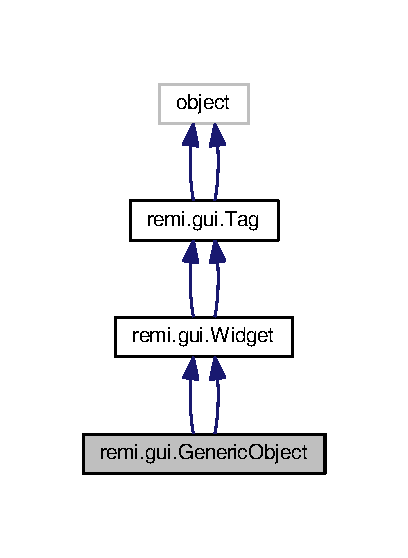
\includegraphics[width=196pt]{d9/d0d/classremi_1_1gui_1_1GenericObject__inherit__graph}
\end{center}
\end{figure}


Collaboration diagram for remi.\+gui.\+Generic\+Object\+:
\nopagebreak
\begin{figure}[H]
\begin{center}
\leavevmode
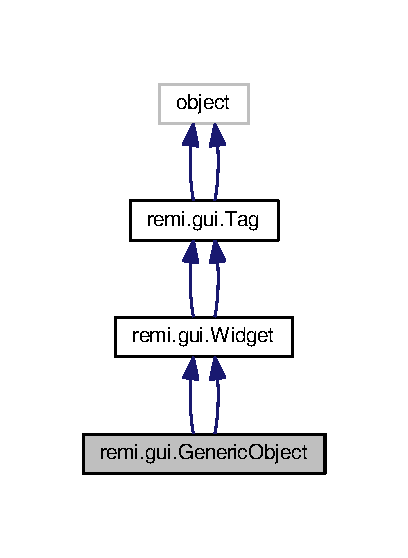
\includegraphics[width=196pt]{de/d07/classremi_1_1gui_1_1GenericObject__coll__graph}
\end{center}
\end{figure}
\subsection*{Public Member Functions}
\begin{DoxyCompactItemize}
\item 
def \hyperlink{classremi_1_1gui_1_1GenericObject_a919ab6921c11385ab2537d732f812e19}{\+\_\+\+\_\+init\+\_\+\+\_\+} (self, filename, kwargs)
\item 
def \hyperlink{classremi_1_1gui_1_1GenericObject_a919ab6921c11385ab2537d732f812e19}{\+\_\+\+\_\+init\+\_\+\+\_\+} (self, filename, kwargs)
\end{DoxyCompactItemize}
\subsection*{Public Attributes}
\begin{DoxyCompactItemize}
\item 
{\bfseries type}\hypertarget{classremi_1_1gui_1_1GenericObject_a1096e15c6de14ca2c7fb5036849f1772}{}\label{classremi_1_1gui_1_1GenericObject_a1096e15c6de14ca2c7fb5036849f1772}

\end{DoxyCompactItemize}
\subsection*{Additional Inherited Members}


\subsection{Detailed Description}
\begin{DoxyVerb}GenericObject widget - allows to show embedded object like pdf,swf..
\end{DoxyVerb}
 

\subsection{Constructor \& Destructor Documentation}
\index{remi\+::gui\+::\+Generic\+Object@{remi\+::gui\+::\+Generic\+Object}!\+\_\+\+\_\+init\+\_\+\+\_\+@{\+\_\+\+\_\+init\+\_\+\+\_\+}}
\index{\+\_\+\+\_\+init\+\_\+\+\_\+@{\+\_\+\+\_\+init\+\_\+\+\_\+}!remi\+::gui\+::\+Generic\+Object@{remi\+::gui\+::\+Generic\+Object}}
\subsubsection[{\texorpdfstring{\+\_\+\+\_\+init\+\_\+\+\_\+(self, filename, kwargs)}{__init__(self, filename, kwargs)}}]{\setlength{\rightskip}{0pt plus 5cm}def remi.\+gui.\+Generic\+Object.\+\_\+\+\_\+init\+\_\+\+\_\+ (
\begin{DoxyParamCaption}
\item[{}]{self, }
\item[{}]{filename, }
\item[{}]{kwargs}
\end{DoxyParamCaption}
)}\hypertarget{classremi_1_1gui_1_1GenericObject_a919ab6921c11385ab2537d732f812e19}{}\label{classremi_1_1gui_1_1GenericObject_a919ab6921c11385ab2537d732f812e19}
\begin{DoxyVerb}Args:
    filename (str): URL
    kwargs: See Widget.__init__()
\end{DoxyVerb}
 \index{remi\+::gui\+::\+Generic\+Object@{remi\+::gui\+::\+Generic\+Object}!\+\_\+\+\_\+init\+\_\+\+\_\+@{\+\_\+\+\_\+init\+\_\+\+\_\+}}
\index{\+\_\+\+\_\+init\+\_\+\+\_\+@{\+\_\+\+\_\+init\+\_\+\+\_\+}!remi\+::gui\+::\+Generic\+Object@{remi\+::gui\+::\+Generic\+Object}}
\subsubsection[{\texorpdfstring{\+\_\+\+\_\+init\+\_\+\+\_\+(self, filename, kwargs)}{__init__(self, filename, kwargs)}}]{\setlength{\rightskip}{0pt plus 5cm}def remi.\+gui.\+Generic\+Object.\+\_\+\+\_\+init\+\_\+\+\_\+ (
\begin{DoxyParamCaption}
\item[{}]{self, }
\item[{}]{filename, }
\item[{}]{kwargs}
\end{DoxyParamCaption}
)}\hypertarget{classremi_1_1gui_1_1GenericObject_a919ab6921c11385ab2537d732f812e19}{}\label{classremi_1_1gui_1_1GenericObject_a919ab6921c11385ab2537d732f812e19}
\begin{DoxyVerb}Args:
    filename (str): URL
    kwargs: See Widget.__init__()
\end{DoxyVerb}
 

The documentation for this class was generated from the following file\+:\begin{DoxyCompactItemize}
\item 
Compiled/\+Server/remi/gui.\+py\end{DoxyCompactItemize}

\hypertarget{classremi_1_1gui_1_1HBox}{}\section{remi.\+gui.\+H\+Box Class Reference}
\label{classremi_1_1gui_1_1HBox}\index{remi.\+gui.\+H\+Box@{remi.\+gui.\+H\+Box}}


Inheritance diagram for remi.\+gui.\+H\+Box\+:
\nopagebreak
\begin{figure}[H]
\begin{center}
\leavevmode
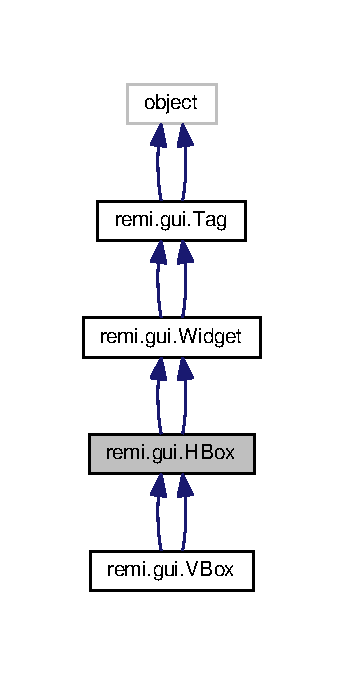
\includegraphics[width=165pt]{d2/de2/classremi_1_1gui_1_1HBox__inherit__graph}
\end{center}
\end{figure}


Collaboration diagram for remi.\+gui.\+H\+Box\+:
\nopagebreak
\begin{figure}[H]
\begin{center}
\leavevmode
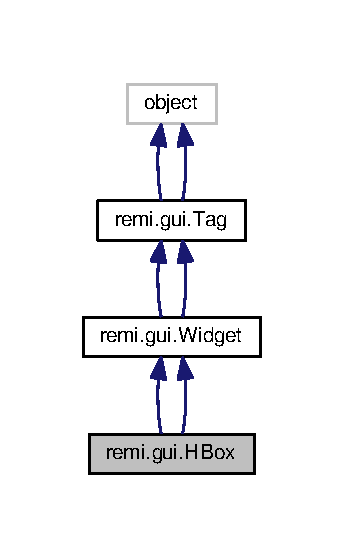
\includegraphics[width=165pt]{d4/df4/classremi_1_1gui_1_1HBox__coll__graph}
\end{center}
\end{figure}
\subsection*{Public Member Functions}
\begin{DoxyCompactItemize}
\item 
def \hyperlink{classremi_1_1gui_1_1HBox_ac92bc687e75b81b270eea9aa68c36e4c}{\+\_\+\+\_\+init\+\_\+\+\_\+} (self, kwargs)
\item 
def \hyperlink{classremi_1_1gui_1_1HBox_a12c4e876e19690415fc6ce3996499fe4}{append} (self, value, key=\textquotesingle{}\textquotesingle{})
\item 
def \hyperlink{classremi_1_1gui_1_1HBox_ac92bc687e75b81b270eea9aa68c36e4c}{\+\_\+\+\_\+init\+\_\+\+\_\+} (self, kwargs)
\item 
def \hyperlink{classremi_1_1gui_1_1HBox_a12c4e876e19690415fc6ce3996499fe4}{append} (self, value, key=\textquotesingle{}\textquotesingle{})
\end{DoxyCompactItemize}
\subsection*{Public Attributes}
\begin{DoxyCompactItemize}
\item 
{\bfseries layout\+\_\+orientation}\hypertarget{classremi_1_1gui_1_1HBox_a89baa42553c214c964106c8059bf8af9}{}\label{classremi_1_1gui_1_1HBox_a89baa42553c214c964106c8059bf8af9}

\end{DoxyCompactItemize}
\subsection*{Additional Inherited Members}


\subsection{Detailed Description}
\begin{DoxyVerb}It contains widget automatically aligning them horizontally.
Does not permit children absolute positioning.

In order to add children to this container, use the append(child, key) function.
The key have to be numeric and determines the children order in the layout.

Note: If you would absolute positioning, use the Widget container instead.
\end{DoxyVerb}
 

\subsection{Constructor \& Destructor Documentation}
\index{remi\+::gui\+::\+H\+Box@{remi\+::gui\+::\+H\+Box}!\+\_\+\+\_\+init\+\_\+\+\_\+@{\+\_\+\+\_\+init\+\_\+\+\_\+}}
\index{\+\_\+\+\_\+init\+\_\+\+\_\+@{\+\_\+\+\_\+init\+\_\+\+\_\+}!remi\+::gui\+::\+H\+Box@{remi\+::gui\+::\+H\+Box}}
\subsubsection[{\texorpdfstring{\+\_\+\+\_\+init\+\_\+\+\_\+(self, kwargs)}{__init__(self, kwargs)}}]{\setlength{\rightskip}{0pt plus 5cm}def remi.\+gui.\+H\+Box.\+\_\+\+\_\+init\+\_\+\+\_\+ (
\begin{DoxyParamCaption}
\item[{}]{self, }
\item[{}]{kwargs}
\end{DoxyParamCaption}
)}\hypertarget{classremi_1_1gui_1_1HBox_ac92bc687e75b81b270eea9aa68c36e4c}{}\label{classremi_1_1gui_1_1HBox_ac92bc687e75b81b270eea9aa68c36e4c}
\begin{DoxyVerb}Args:
    kwargs:
\end{DoxyVerb}
 \index{remi\+::gui\+::\+H\+Box@{remi\+::gui\+::\+H\+Box}!\+\_\+\+\_\+init\+\_\+\+\_\+@{\+\_\+\+\_\+init\+\_\+\+\_\+}}
\index{\+\_\+\+\_\+init\+\_\+\+\_\+@{\+\_\+\+\_\+init\+\_\+\+\_\+}!remi\+::gui\+::\+H\+Box@{remi\+::gui\+::\+H\+Box}}
\subsubsection[{\texorpdfstring{\+\_\+\+\_\+init\+\_\+\+\_\+(self, kwargs)}{__init__(self, kwargs)}}]{\setlength{\rightskip}{0pt plus 5cm}def remi.\+gui.\+H\+Box.\+\_\+\+\_\+init\+\_\+\+\_\+ (
\begin{DoxyParamCaption}
\item[{}]{self, }
\item[{}]{kwargs}
\end{DoxyParamCaption}
)}\hypertarget{classremi_1_1gui_1_1HBox_ac92bc687e75b81b270eea9aa68c36e4c}{}\label{classremi_1_1gui_1_1HBox_ac92bc687e75b81b270eea9aa68c36e4c}
\begin{DoxyVerb}Args:
    kwargs:
\end{DoxyVerb}
 

\subsection{Member Function Documentation}
\index{remi\+::gui\+::\+H\+Box@{remi\+::gui\+::\+H\+Box}!append@{append}}
\index{append@{append}!remi\+::gui\+::\+H\+Box@{remi\+::gui\+::\+H\+Box}}
\subsubsection[{\texorpdfstring{append(self, value, key=\textquotesingle{}\textquotesingle{})}{append(self, value, key='')}}]{\setlength{\rightskip}{0pt plus 5cm}def remi.\+gui.\+H\+Box.\+append (
\begin{DoxyParamCaption}
\item[{}]{self, }
\item[{}]{value, }
\item[{}]{key = {\ttfamily \textquotesingle{}\textquotesingle{}}}
\end{DoxyParamCaption}
)}\hypertarget{classremi_1_1gui_1_1HBox_a12c4e876e19690415fc6ce3996499fe4}{}\label{classremi_1_1gui_1_1HBox_a12c4e876e19690415fc6ce3996499fe4}
\begin{DoxyVerb}It allows to add child widgets to this.
The key allows to access the specific child in this way widget.children[key].
The key have to be numeric and determines the children order in the layout.

Args:
    value (Widget): Child instance to be appended.
    key (str): Unique identifier for the child. If key.isdigit()==True '0' '1'.. the value determines the order
    in the layout
\end{DoxyVerb}
 \index{remi\+::gui\+::\+H\+Box@{remi\+::gui\+::\+H\+Box}!append@{append}}
\index{append@{append}!remi\+::gui\+::\+H\+Box@{remi\+::gui\+::\+H\+Box}}
\subsubsection[{\texorpdfstring{append(self, value, key=\textquotesingle{}\textquotesingle{})}{append(self, value, key='')}}]{\setlength{\rightskip}{0pt plus 5cm}def remi.\+gui.\+H\+Box.\+append (
\begin{DoxyParamCaption}
\item[{}]{self, }
\item[{}]{value, }
\item[{}]{key = {\ttfamily \textquotesingle{}\textquotesingle{}}}
\end{DoxyParamCaption}
)}\hypertarget{classremi_1_1gui_1_1HBox_a12c4e876e19690415fc6ce3996499fe4}{}\label{classremi_1_1gui_1_1HBox_a12c4e876e19690415fc6ce3996499fe4}
\begin{DoxyVerb}It allows to add child widgets to this.
The key allows to access the specific child in this way widget.children[key].
The key have to be numeric and determines the children order in the layout.

Args:
    value (Widget): Child instance to be appended.
    key (str): Unique identifier for the child. If key.isdigit()==True '0' '1'.. the value determines the order
    in the layout
\end{DoxyVerb}
 

The documentation for this class was generated from the following file\+:\begin{DoxyCompactItemize}
\item 
Compiled/\+Server/remi/gui.\+py\end{DoxyCompactItemize}

\hypertarget{classremi_1_1gui_1_1Image}{}\section{remi.\+gui.\+Image Class Reference}
\label{classremi_1_1gui_1_1Image}\index{remi.\+gui.\+Image@{remi.\+gui.\+Image}}


Inheritance diagram for remi.\+gui.\+Image\+:
\nopagebreak
\begin{figure}[H]
\begin{center}
\leavevmode
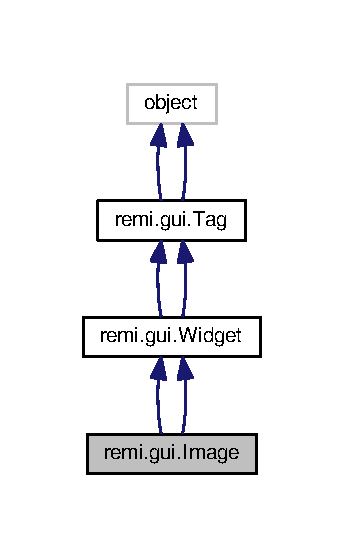
\includegraphics[width=165pt]{d4/dbd/classremi_1_1gui_1_1Image__inherit__graph}
\end{center}
\end{figure}


Collaboration diagram for remi.\+gui.\+Image\+:
\nopagebreak
\begin{figure}[H]
\begin{center}
\leavevmode
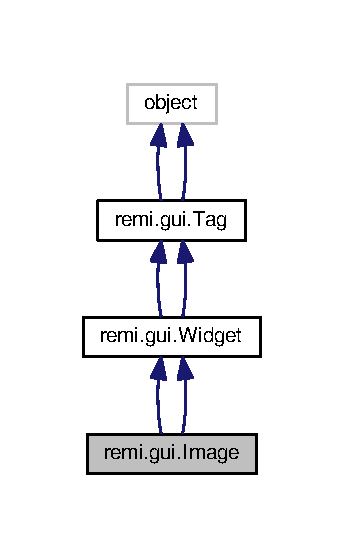
\includegraphics[width=165pt]{d6/d7b/classremi_1_1gui_1_1Image__coll__graph}
\end{center}
\end{figure}
\subsection*{Public Member Functions}
\begin{DoxyCompactItemize}
\item 
def \hyperlink{classremi_1_1gui_1_1Image_a85bf0e4d303e377ba8cf9e8b6100d4c1}{\+\_\+\+\_\+init\+\_\+\+\_\+} (self, filename, kwargs)
\item 
def \hyperlink{classremi_1_1gui_1_1Image_a222d376e090ea59cfbfe0b66e55d2fd4}{set\+\_\+image} (self, filename)
\item 
def \hyperlink{classremi_1_1gui_1_1Image_a85bf0e4d303e377ba8cf9e8b6100d4c1}{\+\_\+\+\_\+init\+\_\+\+\_\+} (self, filename, kwargs)
\item 
def \hyperlink{classremi_1_1gui_1_1Image_a222d376e090ea59cfbfe0b66e55d2fd4}{set\+\_\+image} (self, filename)
\end{DoxyCompactItemize}
\subsection*{Public Attributes}
\begin{DoxyCompactItemize}
\item 
{\bfseries type}\hypertarget{classremi_1_1gui_1_1Image_a55008fa6288d7bf8b33afd53b78bcb2f}{}\label{classremi_1_1gui_1_1Image_a55008fa6288d7bf8b33afd53b78bcb2f}

\end{DoxyCompactItemize}
\subsection*{Additional Inherited Members}


\subsection{Detailed Description}
\begin{DoxyVerb}image widget.\end{DoxyVerb}
 

\subsection{Constructor \& Destructor Documentation}
\index{remi\+::gui\+::\+Image@{remi\+::gui\+::\+Image}!\+\_\+\+\_\+init\+\_\+\+\_\+@{\+\_\+\+\_\+init\+\_\+\+\_\+}}
\index{\+\_\+\+\_\+init\+\_\+\+\_\+@{\+\_\+\+\_\+init\+\_\+\+\_\+}!remi\+::gui\+::\+Image@{remi\+::gui\+::\+Image}}
\subsubsection[{\texorpdfstring{\+\_\+\+\_\+init\+\_\+\+\_\+(self, filename, kwargs)}{__init__(self, filename, kwargs)}}]{\setlength{\rightskip}{0pt plus 5cm}def remi.\+gui.\+Image.\+\_\+\+\_\+init\+\_\+\+\_\+ (
\begin{DoxyParamCaption}
\item[{}]{self, }
\item[{}]{filename, }
\item[{}]{kwargs}
\end{DoxyParamCaption}
)}\hypertarget{classremi_1_1gui_1_1Image_a85bf0e4d303e377ba8cf9e8b6100d4c1}{}\label{classremi_1_1gui_1_1Image_a85bf0e4d303e377ba8cf9e8b6100d4c1}
\begin{DoxyVerb}Args:
    filename (str): an url to an image
    kwargs: See Widget.__init__()
\end{DoxyVerb}
 \index{remi\+::gui\+::\+Image@{remi\+::gui\+::\+Image}!\+\_\+\+\_\+init\+\_\+\+\_\+@{\+\_\+\+\_\+init\+\_\+\+\_\+}}
\index{\+\_\+\+\_\+init\+\_\+\+\_\+@{\+\_\+\+\_\+init\+\_\+\+\_\+}!remi\+::gui\+::\+Image@{remi\+::gui\+::\+Image}}
\subsubsection[{\texorpdfstring{\+\_\+\+\_\+init\+\_\+\+\_\+(self, filename, kwargs)}{__init__(self, filename, kwargs)}}]{\setlength{\rightskip}{0pt plus 5cm}def remi.\+gui.\+Image.\+\_\+\+\_\+init\+\_\+\+\_\+ (
\begin{DoxyParamCaption}
\item[{}]{self, }
\item[{}]{filename, }
\item[{}]{kwargs}
\end{DoxyParamCaption}
)}\hypertarget{classremi_1_1gui_1_1Image_a85bf0e4d303e377ba8cf9e8b6100d4c1}{}\label{classremi_1_1gui_1_1Image_a85bf0e4d303e377ba8cf9e8b6100d4c1}
\begin{DoxyVerb}Args:
    filename (str): an url to an image
    kwargs: See Widget.__init__()
\end{DoxyVerb}
 

\subsection{Member Function Documentation}
\index{remi\+::gui\+::\+Image@{remi\+::gui\+::\+Image}!set\+\_\+image@{set\+\_\+image}}
\index{set\+\_\+image@{set\+\_\+image}!remi\+::gui\+::\+Image@{remi\+::gui\+::\+Image}}
\subsubsection[{\texorpdfstring{set\+\_\+image(self, filename)}{set_image(self, filename)}}]{\setlength{\rightskip}{0pt plus 5cm}def remi.\+gui.\+Image.\+set\+\_\+image (
\begin{DoxyParamCaption}
\item[{}]{self, }
\item[{}]{filename}
\end{DoxyParamCaption}
)}\hypertarget{classremi_1_1gui_1_1Image_a222d376e090ea59cfbfe0b66e55d2fd4}{}\label{classremi_1_1gui_1_1Image_a222d376e090ea59cfbfe0b66e55d2fd4}
\begin{DoxyVerb}Args:
    filename (str): an url to an image
\end{DoxyVerb}
 \index{remi\+::gui\+::\+Image@{remi\+::gui\+::\+Image}!set\+\_\+image@{set\+\_\+image}}
\index{set\+\_\+image@{set\+\_\+image}!remi\+::gui\+::\+Image@{remi\+::gui\+::\+Image}}
\subsubsection[{\texorpdfstring{set\+\_\+image(self, filename)}{set_image(self, filename)}}]{\setlength{\rightskip}{0pt plus 5cm}def remi.\+gui.\+Image.\+set\+\_\+image (
\begin{DoxyParamCaption}
\item[{}]{self, }
\item[{}]{filename}
\end{DoxyParamCaption}
)}\hypertarget{classremi_1_1gui_1_1Image_a222d376e090ea59cfbfe0b66e55d2fd4}{}\label{classremi_1_1gui_1_1Image_a222d376e090ea59cfbfe0b66e55d2fd4}
\begin{DoxyVerb}Args:
    filename (str): an url to an image
\end{DoxyVerb}
 

The documentation for this class was generated from the following file\+:\begin{DoxyCompactItemize}
\item 
Compiled/\+Server/remi/gui.\+py\end{DoxyCompactItemize}

\hypertarget{classremi_1_1gui_1_1Input}{}\section{remi.\+gui.\+Input Class Reference}
\label{classremi_1_1gui_1_1Input}\index{remi.\+gui.\+Input@{remi.\+gui.\+Input}}


Inheritance diagram for remi.\+gui.\+Input\+:
\nopagebreak
\begin{figure}[H]
\begin{center}
\leavevmode
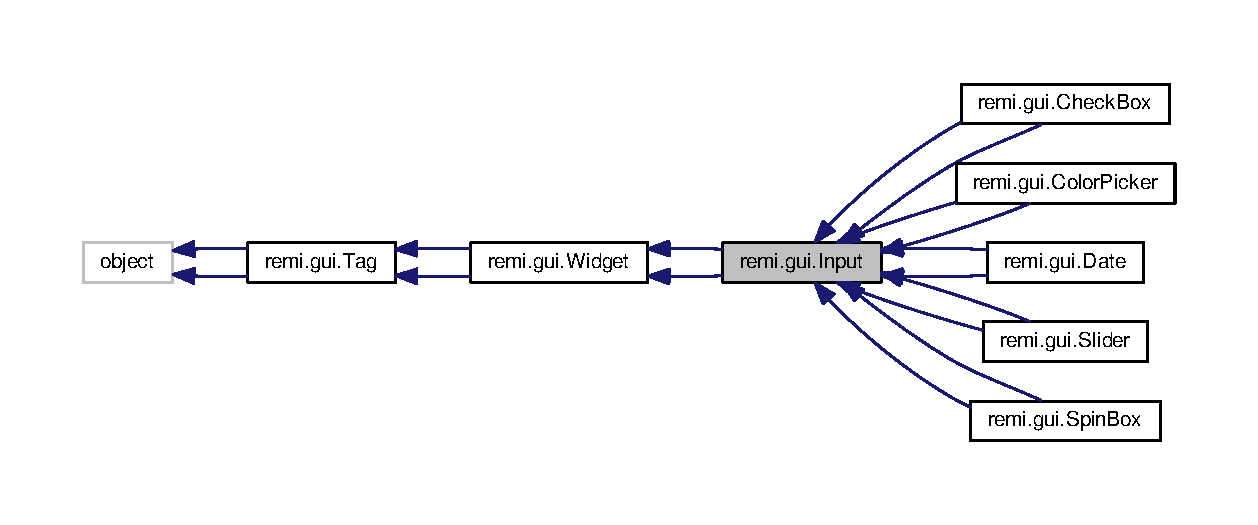
\includegraphics[width=350pt]{d1/d16/classremi_1_1gui_1_1Input__inherit__graph}
\end{center}
\end{figure}


Collaboration diagram for remi.\+gui.\+Input\+:
\nopagebreak
\begin{figure}[H]
\begin{center}
\leavevmode
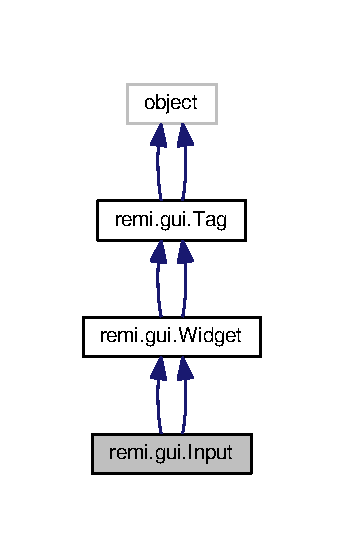
\includegraphics[width=165pt]{d7/d88/classremi_1_1gui_1_1Input__coll__graph}
\end{center}
\end{figure}
\subsection*{Public Member Functions}
\begin{DoxyCompactItemize}
\item 
def \hyperlink{classremi_1_1gui_1_1Input_a7fbd2240680a6a5851b3e6cb4803c702}{\+\_\+\+\_\+init\+\_\+\+\_\+} (self, input\+\_\+type=\textquotesingle{}\textquotesingle{}, default\+\_\+value=\textquotesingle{}\textquotesingle{}, kwargs)
\item 
def \hyperlink{classremi_1_1gui_1_1Input_adf726194a728fbf42b1e3a5832ac39f0}{set\+\_\+value} (self, value)
\item 
def \hyperlink{classremi_1_1gui_1_1Input_ae70594dc1113bb42e74ee2d20ae27896}{get\+\_\+value} (self)
\item 
def \hyperlink{classremi_1_1gui_1_1Input_a05ed9a1c3dcd85ae8b3eb1216b2a6a6a}{onchange} (self, value)
\item 
def \hyperlink{classremi_1_1gui_1_1Input_a094ee901b2fa3915b4c68e2ab40d4bca}{set\+\_\+on\+\_\+change\+\_\+listener} (self, callback, userdata)
\item 
def \hyperlink{classremi_1_1gui_1_1Input_afe721e53146ce0a36f77452fe4d22f6b}{set\+\_\+read\+\_\+only} (self, readonly)
\item 
def \hyperlink{classremi_1_1gui_1_1Input_a7fbd2240680a6a5851b3e6cb4803c702}{\+\_\+\+\_\+init\+\_\+\+\_\+} (self, input\+\_\+type=\textquotesingle{}\textquotesingle{}, default\+\_\+value=\textquotesingle{}\textquotesingle{}, kwargs)
\item 
def \hyperlink{classremi_1_1gui_1_1Input_adf726194a728fbf42b1e3a5832ac39f0}{set\+\_\+value} (self, value)
\item 
def \hyperlink{classremi_1_1gui_1_1Input_ae70594dc1113bb42e74ee2d20ae27896}{get\+\_\+value} (self)
\item 
def \hyperlink{classremi_1_1gui_1_1Input_a05ed9a1c3dcd85ae8b3eb1216b2a6a6a}{onchange} (self, value)
\item 
def \hyperlink{classremi_1_1gui_1_1Input_a094ee901b2fa3915b4c68e2ab40d4bca}{set\+\_\+on\+\_\+change\+\_\+listener} (self, callback, userdata)
\item 
def \hyperlink{classremi_1_1gui_1_1Input_afe721e53146ce0a36f77452fe4d22f6b}{set\+\_\+read\+\_\+only} (self, readonly)
\end{DoxyCompactItemize}
\subsection*{Public Attributes}
\begin{DoxyCompactItemize}
\item 
{\bfseries type}\hypertarget{classremi_1_1gui_1_1Input_a77c5b2fea1826a5237e8d24645182343}{}\label{classremi_1_1gui_1_1Input_a77c5b2fea1826a5237e8d24645182343}

\end{DoxyCompactItemize}
\subsection*{Additional Inherited Members}


\subsection{Detailed Description}
\begin{DoxyVerb}\end{DoxyVerb}
 

\subsection{Constructor \& Destructor Documentation}
\index{remi\+::gui\+::\+Input@{remi\+::gui\+::\+Input}!\+\_\+\+\_\+init\+\_\+\+\_\+@{\+\_\+\+\_\+init\+\_\+\+\_\+}}
\index{\+\_\+\+\_\+init\+\_\+\+\_\+@{\+\_\+\+\_\+init\+\_\+\+\_\+}!remi\+::gui\+::\+Input@{remi\+::gui\+::\+Input}}
\subsubsection[{\texorpdfstring{\+\_\+\+\_\+init\+\_\+\+\_\+(self, input\+\_\+type=\textquotesingle{}\textquotesingle{}, default\+\_\+value=\textquotesingle{}\textquotesingle{}, kwargs)}{__init__(self, input_type='', default_value='', kwargs)}}]{\setlength{\rightskip}{0pt plus 5cm}def remi.\+gui.\+Input.\+\_\+\+\_\+init\+\_\+\+\_\+ (
\begin{DoxyParamCaption}
\item[{}]{self, }
\item[{}]{input\+\_\+type = {\ttfamily \textquotesingle{}\textquotesingle{}}, }
\item[{}]{default\+\_\+value = {\ttfamily \textquotesingle{}\textquotesingle{}}, }
\item[{}]{kwargs}
\end{DoxyParamCaption}
)}\hypertarget{classremi_1_1gui_1_1Input_a7fbd2240680a6a5851b3e6cb4803c702}{}\label{classremi_1_1gui_1_1Input_a7fbd2240680a6a5851b3e6cb4803c702}
\begin{DoxyVerb}Args:
    input_type (str): HTML5 input type
    default_value (str):
    kwargs: See Widget.__init__()
\end{DoxyVerb}
 \index{remi\+::gui\+::\+Input@{remi\+::gui\+::\+Input}!\+\_\+\+\_\+init\+\_\+\+\_\+@{\+\_\+\+\_\+init\+\_\+\+\_\+}}
\index{\+\_\+\+\_\+init\+\_\+\+\_\+@{\+\_\+\+\_\+init\+\_\+\+\_\+}!remi\+::gui\+::\+Input@{remi\+::gui\+::\+Input}}
\subsubsection[{\texorpdfstring{\+\_\+\+\_\+init\+\_\+\+\_\+(self, input\+\_\+type=\textquotesingle{}\textquotesingle{}, default\+\_\+value=\textquotesingle{}\textquotesingle{}, kwargs)}{__init__(self, input_type='', default_value='', kwargs)}}]{\setlength{\rightskip}{0pt plus 5cm}def remi.\+gui.\+Input.\+\_\+\+\_\+init\+\_\+\+\_\+ (
\begin{DoxyParamCaption}
\item[{}]{self, }
\item[{}]{input\+\_\+type = {\ttfamily \textquotesingle{}\textquotesingle{}}, }
\item[{}]{default\+\_\+value = {\ttfamily \textquotesingle{}\textquotesingle{}}, }
\item[{}]{kwargs}
\end{DoxyParamCaption}
)}\hypertarget{classremi_1_1gui_1_1Input_a7fbd2240680a6a5851b3e6cb4803c702}{}\label{classremi_1_1gui_1_1Input_a7fbd2240680a6a5851b3e6cb4803c702}
\begin{DoxyVerb}Args:
    input_type (str): HTML5 input type
    default_value (str):
    kwargs: See Widget.__init__()
\end{DoxyVerb}
 

\subsection{Member Function Documentation}
\index{remi\+::gui\+::\+Input@{remi\+::gui\+::\+Input}!get\+\_\+value@{get\+\_\+value}}
\index{get\+\_\+value@{get\+\_\+value}!remi\+::gui\+::\+Input@{remi\+::gui\+::\+Input}}
\subsubsection[{\texorpdfstring{get\+\_\+value(self)}{get_value(self)}}]{\setlength{\rightskip}{0pt plus 5cm}def remi.\+gui.\+Input.\+get\+\_\+value (
\begin{DoxyParamCaption}
\item[{}]{self}
\end{DoxyParamCaption}
)}\hypertarget{classremi_1_1gui_1_1Input_ae70594dc1113bb42e74ee2d20ae27896}{}\label{classremi_1_1gui_1_1Input_ae70594dc1113bb42e74ee2d20ae27896}
\begin{DoxyVerb}returns the new text value.\end{DoxyVerb}
 \index{remi\+::gui\+::\+Input@{remi\+::gui\+::\+Input}!get\+\_\+value@{get\+\_\+value}}
\index{get\+\_\+value@{get\+\_\+value}!remi\+::gui\+::\+Input@{remi\+::gui\+::\+Input}}
\subsubsection[{\texorpdfstring{get\+\_\+value(self)}{get_value(self)}}]{\setlength{\rightskip}{0pt plus 5cm}def remi.\+gui.\+Input.\+get\+\_\+value (
\begin{DoxyParamCaption}
\item[{}]{self}
\end{DoxyParamCaption}
)}\hypertarget{classremi_1_1gui_1_1Input_ae70594dc1113bb42e74ee2d20ae27896}{}\label{classremi_1_1gui_1_1Input_ae70594dc1113bb42e74ee2d20ae27896}
\begin{DoxyVerb}returns the new text value.\end{DoxyVerb}
 \index{remi\+::gui\+::\+Input@{remi\+::gui\+::\+Input}!onchange@{onchange}}
\index{onchange@{onchange}!remi\+::gui\+::\+Input@{remi\+::gui\+::\+Input}}
\subsubsection[{\texorpdfstring{onchange(self, value)}{onchange(self, value)}}]{\setlength{\rightskip}{0pt plus 5cm}def remi.\+gui.\+Input.\+onchange (
\begin{DoxyParamCaption}
\item[{}]{self, }
\item[{}]{value}
\end{DoxyParamCaption}
)}\hypertarget{classremi_1_1gui_1_1Input_a05ed9a1c3dcd85ae8b3eb1216b2a6a6a}{}\label{classremi_1_1gui_1_1Input_a05ed9a1c3dcd85ae8b3eb1216b2a6a6a}
\begin{DoxyVerb}Args:
    value:

Returns:\end{DoxyVerb}
 \index{remi\+::gui\+::\+Input@{remi\+::gui\+::\+Input}!onchange@{onchange}}
\index{onchange@{onchange}!remi\+::gui\+::\+Input@{remi\+::gui\+::\+Input}}
\subsubsection[{\texorpdfstring{onchange(self, value)}{onchange(self, value)}}]{\setlength{\rightskip}{0pt plus 5cm}def remi.\+gui.\+Input.\+onchange (
\begin{DoxyParamCaption}
\item[{}]{self, }
\item[{}]{value}
\end{DoxyParamCaption}
)}\hypertarget{classremi_1_1gui_1_1Input_a05ed9a1c3dcd85ae8b3eb1216b2a6a6a}{}\label{classremi_1_1gui_1_1Input_a05ed9a1c3dcd85ae8b3eb1216b2a6a6a}
\begin{DoxyVerb}Args:
    value:

Returns:\end{DoxyVerb}
 \index{remi\+::gui\+::\+Input@{remi\+::gui\+::\+Input}!set\+\_\+on\+\_\+change\+\_\+listener@{set\+\_\+on\+\_\+change\+\_\+listener}}
\index{set\+\_\+on\+\_\+change\+\_\+listener@{set\+\_\+on\+\_\+change\+\_\+listener}!remi\+::gui\+::\+Input@{remi\+::gui\+::\+Input}}
\subsubsection[{\texorpdfstring{set\+\_\+on\+\_\+change\+\_\+listener(self, callback, userdata)}{set_on_change_listener(self, callback, userdata)}}]{\setlength{\rightskip}{0pt plus 5cm}def remi.\+gui.\+Input.\+set\+\_\+on\+\_\+change\+\_\+listener (
\begin{DoxyParamCaption}
\item[{}]{self, }
\item[{}]{callback, }
\item[{}]{userdata}
\end{DoxyParamCaption}
)}\hypertarget{classremi_1_1gui_1_1Input_a094ee901b2fa3915b4c68e2ab40d4bca}{}\label{classremi_1_1gui_1_1Input_a094ee901b2fa3915b4c68e2ab40d4bca}
\begin{DoxyVerb}Register the listener for the onchange event.

Note: the listener prototype have to be in the form on_input_changed(self, widget, value).
\end{DoxyVerb}
 \index{remi\+::gui\+::\+Input@{remi\+::gui\+::\+Input}!set\+\_\+on\+\_\+change\+\_\+listener@{set\+\_\+on\+\_\+change\+\_\+listener}}
\index{set\+\_\+on\+\_\+change\+\_\+listener@{set\+\_\+on\+\_\+change\+\_\+listener}!remi\+::gui\+::\+Input@{remi\+::gui\+::\+Input}}
\subsubsection[{\texorpdfstring{set\+\_\+on\+\_\+change\+\_\+listener(self, callback, userdata)}{set_on_change_listener(self, callback, userdata)}}]{\setlength{\rightskip}{0pt plus 5cm}def remi.\+gui.\+Input.\+set\+\_\+on\+\_\+change\+\_\+listener (
\begin{DoxyParamCaption}
\item[{}]{self, }
\item[{}]{callback, }
\item[{}]{userdata}
\end{DoxyParamCaption}
)}\hypertarget{classremi_1_1gui_1_1Input_a094ee901b2fa3915b4c68e2ab40d4bca}{}\label{classremi_1_1gui_1_1Input_a094ee901b2fa3915b4c68e2ab40d4bca}
\begin{DoxyVerb}Register the listener for the onchange event.

Note: the listener prototype have to be in the form on_input_changed(self, widget, value).
\end{DoxyVerb}
 \index{remi\+::gui\+::\+Input@{remi\+::gui\+::\+Input}!set\+\_\+read\+\_\+only@{set\+\_\+read\+\_\+only}}
\index{set\+\_\+read\+\_\+only@{set\+\_\+read\+\_\+only}!remi\+::gui\+::\+Input@{remi\+::gui\+::\+Input}}
\subsubsection[{\texorpdfstring{set\+\_\+read\+\_\+only(self, readonly)}{set_read_only(self, readonly)}}]{\setlength{\rightskip}{0pt plus 5cm}def remi.\+gui.\+Input.\+set\+\_\+read\+\_\+only (
\begin{DoxyParamCaption}
\item[{}]{self, }
\item[{}]{readonly}
\end{DoxyParamCaption}
)}\hypertarget{classremi_1_1gui_1_1Input_afe721e53146ce0a36f77452fe4d22f6b}{}\label{classremi_1_1gui_1_1Input_afe721e53146ce0a36f77452fe4d22f6b}
\begin{DoxyVerb}Args:
    readonly:
\end{DoxyVerb}
 \index{remi\+::gui\+::\+Input@{remi\+::gui\+::\+Input}!set\+\_\+read\+\_\+only@{set\+\_\+read\+\_\+only}}
\index{set\+\_\+read\+\_\+only@{set\+\_\+read\+\_\+only}!remi\+::gui\+::\+Input@{remi\+::gui\+::\+Input}}
\subsubsection[{\texorpdfstring{set\+\_\+read\+\_\+only(self, readonly)}{set_read_only(self, readonly)}}]{\setlength{\rightskip}{0pt plus 5cm}def remi.\+gui.\+Input.\+set\+\_\+read\+\_\+only (
\begin{DoxyParamCaption}
\item[{}]{self, }
\item[{}]{readonly}
\end{DoxyParamCaption}
)}\hypertarget{classremi_1_1gui_1_1Input_afe721e53146ce0a36f77452fe4d22f6b}{}\label{classremi_1_1gui_1_1Input_afe721e53146ce0a36f77452fe4d22f6b}
\begin{DoxyVerb}Args:
    readonly:
\end{DoxyVerb}
 \index{remi\+::gui\+::\+Input@{remi\+::gui\+::\+Input}!set\+\_\+value@{set\+\_\+value}}
\index{set\+\_\+value@{set\+\_\+value}!remi\+::gui\+::\+Input@{remi\+::gui\+::\+Input}}
\subsubsection[{\texorpdfstring{set\+\_\+value(self, value)}{set_value(self, value)}}]{\setlength{\rightskip}{0pt plus 5cm}def remi.\+gui.\+Input.\+set\+\_\+value (
\begin{DoxyParamCaption}
\item[{}]{self, }
\item[{}]{value}
\end{DoxyParamCaption}
)}\hypertarget{classremi_1_1gui_1_1Input_adf726194a728fbf42b1e3a5832ac39f0}{}\label{classremi_1_1gui_1_1Input_adf726194a728fbf42b1e3a5832ac39f0}
\begin{DoxyVerb}Args:
    value:
\end{DoxyVerb}
 \index{remi\+::gui\+::\+Input@{remi\+::gui\+::\+Input}!set\+\_\+value@{set\+\_\+value}}
\index{set\+\_\+value@{set\+\_\+value}!remi\+::gui\+::\+Input@{remi\+::gui\+::\+Input}}
\subsubsection[{\texorpdfstring{set\+\_\+value(self, value)}{set_value(self, value)}}]{\setlength{\rightskip}{0pt plus 5cm}def remi.\+gui.\+Input.\+set\+\_\+value (
\begin{DoxyParamCaption}
\item[{}]{self, }
\item[{}]{value}
\end{DoxyParamCaption}
)}\hypertarget{classremi_1_1gui_1_1Input_adf726194a728fbf42b1e3a5832ac39f0}{}\label{classremi_1_1gui_1_1Input_adf726194a728fbf42b1e3a5832ac39f0}
\begin{DoxyVerb}Args:
    value:
\end{DoxyVerb}
 

The documentation for this class was generated from the following file\+:\begin{DoxyCompactItemize}
\item 
Compiled/\+Server/remi/gui.\+py\end{DoxyCompactItemize}

\hypertarget{classremi_1_1gui_1_1InputDialog}{}\section{remi.\+gui.\+Input\+Dialog Class Reference}
\label{classremi_1_1gui_1_1InputDialog}\index{remi.\+gui.\+Input\+Dialog@{remi.\+gui.\+Input\+Dialog}}


Inheritance diagram for remi.\+gui.\+Input\+Dialog\+:
\nopagebreak
\begin{figure}[H]
\begin{center}
\leavevmode
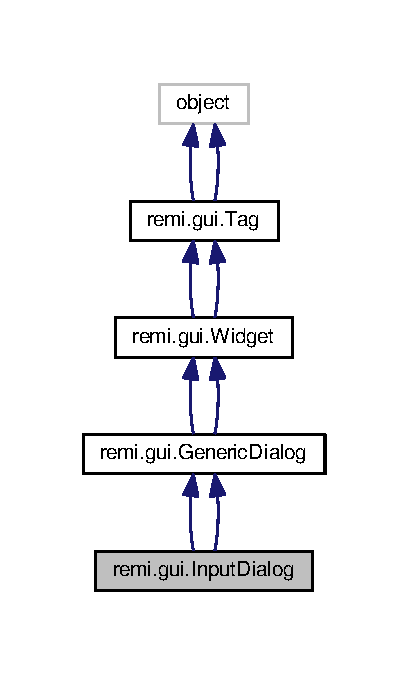
\includegraphics[width=196pt]{da/dbf/classremi_1_1gui_1_1InputDialog__inherit__graph}
\end{center}
\end{figure}


Collaboration diagram for remi.\+gui.\+Input\+Dialog\+:
\nopagebreak
\begin{figure}[H]
\begin{center}
\leavevmode
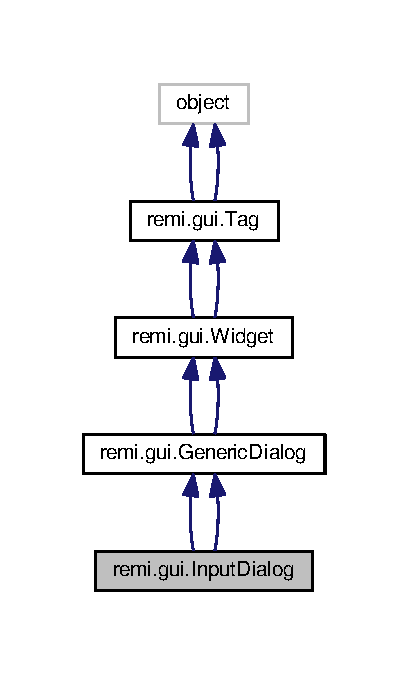
\includegraphics[width=196pt]{da/df1/classremi_1_1gui_1_1InputDialog__coll__graph}
\end{center}
\end{figure}
\subsection*{Public Member Functions}
\begin{DoxyCompactItemize}
\item 
def \hyperlink{classremi_1_1gui_1_1InputDialog_afd73c84c493d65a00f8ff444102ae2cc}{\+\_\+\+\_\+init\+\_\+\+\_\+} (self, title=\textquotesingle{}Title\textquotesingle{}, message=\textquotesingle{}Message\textquotesingle{}, initial\+\_\+value=\textquotesingle{}\textquotesingle{}, kwargs)
\item 
def \hyperlink{classremi_1_1gui_1_1InputDialog_a61b1845d77de3df8dfc27f67b33c617c}{on\+\_\+text\+\_\+enter\+\_\+listener} (self, widget, value)
\item 
def \hyperlink{classremi_1_1gui_1_1InputDialog_a65b20b4e39fdd759fbd47ea081a9b3cd}{confirm\+\_\+value} (self, widget)
\item 
def \hyperlink{classremi_1_1gui_1_1InputDialog_a54fbc140f28297132cf4e7f4a0663e82}{set\+\_\+on\+\_\+confirm\+\_\+value\+\_\+listener} (self, callback, userdata)
\item 
def \hyperlink{classremi_1_1gui_1_1InputDialog_afd73c84c493d65a00f8ff444102ae2cc}{\+\_\+\+\_\+init\+\_\+\+\_\+} (self, title=\textquotesingle{}Title\textquotesingle{}, message=\textquotesingle{}Message\textquotesingle{}, initial\+\_\+value=\textquotesingle{}\textquotesingle{}, kwargs)
\item 
def \hyperlink{classremi_1_1gui_1_1InputDialog_a61b1845d77de3df8dfc27f67b33c617c}{on\+\_\+text\+\_\+enter\+\_\+listener} (self, widget, value)
\item 
def \hyperlink{classremi_1_1gui_1_1InputDialog_a65b20b4e39fdd759fbd47ea081a9b3cd}{confirm\+\_\+value} (self, widget)
\item 
def \hyperlink{classremi_1_1gui_1_1InputDialog_a54fbc140f28297132cf4e7f4a0663e82}{set\+\_\+on\+\_\+confirm\+\_\+value\+\_\+listener} (self, callback, userdata)
\end{DoxyCompactItemize}
\subsection*{Public Attributes}
\begin{DoxyCompactItemize}
\item 
{\bfseries input\+Text}\hypertarget{classremi_1_1gui_1_1InputDialog_a7c1d36c3c62dffbd128d79d5c589de13}{}\label{classremi_1_1gui_1_1InputDialog_a7c1d36c3c62dffbd128d79d5c589de13}

\end{DoxyCompactItemize}
\subsection*{Static Public Attributes}
\begin{DoxyCompactItemize}
\item 
string {\bfseries E\+V\+E\+N\+T\+\_\+\+O\+N\+C\+O\+N\+F\+I\+R\+M\+V\+A\+L\+UE} = \textquotesingle{}\hyperlink{classremi_1_1gui_1_1InputDialog_a65b20b4e39fdd759fbd47ea081a9b3cd}{confirm\+\_\+value}\textquotesingle{}\hypertarget{classremi_1_1gui_1_1InputDialog_a02248849678e75014ee54e297c0b5585}{}\label{classremi_1_1gui_1_1InputDialog_a02248849678e75014ee54e297c0b5585}

\end{DoxyCompactItemize}


\subsection{Detailed Description}
\begin{DoxyVerb}Input Dialog widget. It can be used to query simple and short textual input to the user.
The user can confirm or dismiss the dialog with the common buttons Cancel/Ok.
The Ok button click or the ENTER key pression emits the 'confirm_dialog' event. Register the listener to it
with set_on_confirm_dialog_listener.
The Cancel button emits the 'cancel_dialog' event. Register the listener to it with set_on_cancel_dialog_listener.
\end{DoxyVerb}
 

\subsection{Constructor \& Destructor Documentation}
\index{remi\+::gui\+::\+Input\+Dialog@{remi\+::gui\+::\+Input\+Dialog}!\+\_\+\+\_\+init\+\_\+\+\_\+@{\+\_\+\+\_\+init\+\_\+\+\_\+}}
\index{\+\_\+\+\_\+init\+\_\+\+\_\+@{\+\_\+\+\_\+init\+\_\+\+\_\+}!remi\+::gui\+::\+Input\+Dialog@{remi\+::gui\+::\+Input\+Dialog}}
\subsubsection[{\texorpdfstring{\+\_\+\+\_\+init\+\_\+\+\_\+(self, title=\textquotesingle{}\+Title\textquotesingle{}, message=\textquotesingle{}\+Message\textquotesingle{}, initial\+\_\+value=\textquotesingle{}\textquotesingle{}, kwargs)}{__init__(self, title='Title', message='Message', initial_value='', kwargs)}}]{\setlength{\rightskip}{0pt plus 5cm}def remi.\+gui.\+Input\+Dialog.\+\_\+\+\_\+init\+\_\+\+\_\+ (
\begin{DoxyParamCaption}
\item[{}]{self, }
\item[{}]{title = {\ttfamily \textquotesingle{}Title\textquotesingle{}}, }
\item[{}]{message = {\ttfamily \textquotesingle{}Message\textquotesingle{}}, }
\item[{}]{initial\+\_\+value = {\ttfamily \textquotesingle{}\textquotesingle{}}, }
\item[{}]{kwargs}
\end{DoxyParamCaption}
)}\hypertarget{classremi_1_1gui_1_1InputDialog_afd73c84c493d65a00f8ff444102ae2cc}{}\label{classremi_1_1gui_1_1InputDialog_afd73c84c493d65a00f8ff444102ae2cc}
\begin{DoxyVerb}Args:
    title (str): The title of the dialog.
    message (str): The message description.
    initial_value (str): The default content for the TextInput field.
    kwargs: See Widget.__init__()
\end{DoxyVerb}
 \index{remi\+::gui\+::\+Input\+Dialog@{remi\+::gui\+::\+Input\+Dialog}!\+\_\+\+\_\+init\+\_\+\+\_\+@{\+\_\+\+\_\+init\+\_\+\+\_\+}}
\index{\+\_\+\+\_\+init\+\_\+\+\_\+@{\+\_\+\+\_\+init\+\_\+\+\_\+}!remi\+::gui\+::\+Input\+Dialog@{remi\+::gui\+::\+Input\+Dialog}}
\subsubsection[{\texorpdfstring{\+\_\+\+\_\+init\+\_\+\+\_\+(self, title=\textquotesingle{}\+Title\textquotesingle{}, message=\textquotesingle{}\+Message\textquotesingle{}, initial\+\_\+value=\textquotesingle{}\textquotesingle{}, kwargs)}{__init__(self, title='Title', message='Message', initial_value='', kwargs)}}]{\setlength{\rightskip}{0pt plus 5cm}def remi.\+gui.\+Input\+Dialog.\+\_\+\+\_\+init\+\_\+\+\_\+ (
\begin{DoxyParamCaption}
\item[{}]{self, }
\item[{}]{title = {\ttfamily \textquotesingle{}Title\textquotesingle{}}, }
\item[{}]{message = {\ttfamily \textquotesingle{}Message\textquotesingle{}}, }
\item[{}]{initial\+\_\+value = {\ttfamily \textquotesingle{}\textquotesingle{}}, }
\item[{}]{kwargs}
\end{DoxyParamCaption}
)}\hypertarget{classremi_1_1gui_1_1InputDialog_afd73c84c493d65a00f8ff444102ae2cc}{}\label{classremi_1_1gui_1_1InputDialog_afd73c84c493d65a00f8ff444102ae2cc}
\begin{DoxyVerb}Args:
    title (str): The title of the dialog.
    message (str): The message description.
    initial_value (str): The default content for the TextInput field.
    kwargs: See Widget.__init__()
\end{DoxyVerb}
 

\subsection{Member Function Documentation}
\index{remi\+::gui\+::\+Input\+Dialog@{remi\+::gui\+::\+Input\+Dialog}!confirm\+\_\+value@{confirm\+\_\+value}}
\index{confirm\+\_\+value@{confirm\+\_\+value}!remi\+::gui\+::\+Input\+Dialog@{remi\+::gui\+::\+Input\+Dialog}}
\subsubsection[{\texorpdfstring{confirm\+\_\+value(self, widget)}{confirm_value(self, widget)}}]{\setlength{\rightskip}{0pt plus 5cm}def remi.\+gui.\+Input\+Dialog.\+confirm\+\_\+value (
\begin{DoxyParamCaption}
\item[{}]{self, }
\item[{}]{widget}
\end{DoxyParamCaption}
)}\hypertarget{classremi_1_1gui_1_1InputDialog_a65b20b4e39fdd759fbd47ea081a9b3cd}{}\label{classremi_1_1gui_1_1InputDialog_a65b20b4e39fdd759fbd47ea081a9b3cd}
\begin{DoxyVerb}Event called pressing on OK button.\end{DoxyVerb}
 \index{remi\+::gui\+::\+Input\+Dialog@{remi\+::gui\+::\+Input\+Dialog}!confirm\+\_\+value@{confirm\+\_\+value}}
\index{confirm\+\_\+value@{confirm\+\_\+value}!remi\+::gui\+::\+Input\+Dialog@{remi\+::gui\+::\+Input\+Dialog}}
\subsubsection[{\texorpdfstring{confirm\+\_\+value(self, widget)}{confirm_value(self, widget)}}]{\setlength{\rightskip}{0pt plus 5cm}def remi.\+gui.\+Input\+Dialog.\+confirm\+\_\+value (
\begin{DoxyParamCaption}
\item[{}]{self, }
\item[{}]{widget}
\end{DoxyParamCaption}
)}\hypertarget{classremi_1_1gui_1_1InputDialog_a65b20b4e39fdd759fbd47ea081a9b3cd}{}\label{classremi_1_1gui_1_1InputDialog_a65b20b4e39fdd759fbd47ea081a9b3cd}
\begin{DoxyVerb}Event called pressing on OK button.\end{DoxyVerb}
 \index{remi\+::gui\+::\+Input\+Dialog@{remi\+::gui\+::\+Input\+Dialog}!on\+\_\+text\+\_\+enter\+\_\+listener@{on\+\_\+text\+\_\+enter\+\_\+listener}}
\index{on\+\_\+text\+\_\+enter\+\_\+listener@{on\+\_\+text\+\_\+enter\+\_\+listener}!remi\+::gui\+::\+Input\+Dialog@{remi\+::gui\+::\+Input\+Dialog}}
\subsubsection[{\texorpdfstring{on\+\_\+text\+\_\+enter\+\_\+listener(self, widget, value)}{on_text_enter_listener(self, widget, value)}}]{\setlength{\rightskip}{0pt plus 5cm}def remi.\+gui.\+Input\+Dialog.\+on\+\_\+text\+\_\+enter\+\_\+listener (
\begin{DoxyParamCaption}
\item[{}]{self, }
\item[{}]{widget, }
\item[{}]{value}
\end{DoxyParamCaption}
)}\hypertarget{classremi_1_1gui_1_1InputDialog_a61b1845d77de3df8dfc27f67b33c617c}{}\label{classremi_1_1gui_1_1InputDialog_a61b1845d77de3df8dfc27f67b33c617c}
\begin{DoxyVerb}event called pressing on ENTER key.

propagates the string content of the input field
\end{DoxyVerb}
 \index{remi\+::gui\+::\+Input\+Dialog@{remi\+::gui\+::\+Input\+Dialog}!on\+\_\+text\+\_\+enter\+\_\+listener@{on\+\_\+text\+\_\+enter\+\_\+listener}}
\index{on\+\_\+text\+\_\+enter\+\_\+listener@{on\+\_\+text\+\_\+enter\+\_\+listener}!remi\+::gui\+::\+Input\+Dialog@{remi\+::gui\+::\+Input\+Dialog}}
\subsubsection[{\texorpdfstring{on\+\_\+text\+\_\+enter\+\_\+listener(self, widget, value)}{on_text_enter_listener(self, widget, value)}}]{\setlength{\rightskip}{0pt plus 5cm}def remi.\+gui.\+Input\+Dialog.\+on\+\_\+text\+\_\+enter\+\_\+listener (
\begin{DoxyParamCaption}
\item[{}]{self, }
\item[{}]{widget, }
\item[{}]{value}
\end{DoxyParamCaption}
)}\hypertarget{classremi_1_1gui_1_1InputDialog_a61b1845d77de3df8dfc27f67b33c617c}{}\label{classremi_1_1gui_1_1InputDialog_a61b1845d77de3df8dfc27f67b33c617c}
\begin{DoxyVerb}event called pressing on ENTER key.

propagates the string content of the input field
\end{DoxyVerb}
 \index{remi\+::gui\+::\+Input\+Dialog@{remi\+::gui\+::\+Input\+Dialog}!set\+\_\+on\+\_\+confirm\+\_\+value\+\_\+listener@{set\+\_\+on\+\_\+confirm\+\_\+value\+\_\+listener}}
\index{set\+\_\+on\+\_\+confirm\+\_\+value\+\_\+listener@{set\+\_\+on\+\_\+confirm\+\_\+value\+\_\+listener}!remi\+::gui\+::\+Input\+Dialog@{remi\+::gui\+::\+Input\+Dialog}}
\subsubsection[{\texorpdfstring{set\+\_\+on\+\_\+confirm\+\_\+value\+\_\+listener(self, callback, userdata)}{set_on_confirm_value_listener(self, callback, userdata)}}]{\setlength{\rightskip}{0pt plus 5cm}def remi.\+gui.\+Input\+Dialog.\+set\+\_\+on\+\_\+confirm\+\_\+value\+\_\+listener (
\begin{DoxyParamCaption}
\item[{}]{self, }
\item[{}]{callback, }
\item[{}]{userdata}
\end{DoxyParamCaption}
)}\hypertarget{classremi_1_1gui_1_1InputDialog_a54fbc140f28297132cf4e7f4a0663e82}{}\label{classremi_1_1gui_1_1InputDialog_a54fbc140f28297132cf4e7f4a0663e82}
\begin{DoxyVerb}Registers the listener for the InputDialog.confirm_value event.

Note: The prototype of the listener have to be like my_on_confirm_dialog(self, widget, confirmed_value), where
    confirmed_value is the text content of the input field.

Args:
    callback (function): Callback function pointer.
\end{DoxyVerb}
 \index{remi\+::gui\+::\+Input\+Dialog@{remi\+::gui\+::\+Input\+Dialog}!set\+\_\+on\+\_\+confirm\+\_\+value\+\_\+listener@{set\+\_\+on\+\_\+confirm\+\_\+value\+\_\+listener}}
\index{set\+\_\+on\+\_\+confirm\+\_\+value\+\_\+listener@{set\+\_\+on\+\_\+confirm\+\_\+value\+\_\+listener}!remi\+::gui\+::\+Input\+Dialog@{remi\+::gui\+::\+Input\+Dialog}}
\subsubsection[{\texorpdfstring{set\+\_\+on\+\_\+confirm\+\_\+value\+\_\+listener(self, callback, userdata)}{set_on_confirm_value_listener(self, callback, userdata)}}]{\setlength{\rightskip}{0pt plus 5cm}def remi.\+gui.\+Input\+Dialog.\+set\+\_\+on\+\_\+confirm\+\_\+value\+\_\+listener (
\begin{DoxyParamCaption}
\item[{}]{self, }
\item[{}]{callback, }
\item[{}]{userdata}
\end{DoxyParamCaption}
)}\hypertarget{classremi_1_1gui_1_1InputDialog_a54fbc140f28297132cf4e7f4a0663e82}{}\label{classremi_1_1gui_1_1InputDialog_a54fbc140f28297132cf4e7f4a0663e82}
\begin{DoxyVerb}Registers the listener for the InputDialog.confirm_value event.

Note: The prototype of the listener have to be like my_on_confirm_dialog(self, widget, confirmed_value), where
    confirmed_value is the text content of the input field.

Args:
    callback (function): Callback function pointer.
\end{DoxyVerb}
 

The documentation for this class was generated from the following file\+:\begin{DoxyCompactItemize}
\item 
Compiled/\+Server/remi/gui.\+py\end{DoxyCompactItemize}

\hypertarget{classpy__backend_1_1ServerInteract_1_1interface}{}\section{py\+\_\+backend.\+Server\+Interact.\+interface Class Reference}
\label{classpy__backend_1_1ServerInteract_1_1interface}\index{py\+\_\+backend.\+Server\+Interact.\+interface@{py\+\_\+backend.\+Server\+Interact.\+interface}}
\subsection*{Public Member Functions}
\begin{DoxyCompactItemize}
\item 
def \hyperlink{classpy__backend_1_1ServerInteract_1_1interface_a23c925529e15f6826f72220bbc93fb41}{\+\_\+\+\_\+init\+\_\+\+\_\+} (self, ip, port)
\item 
def \hyperlink{classpy__backend_1_1ServerInteract_1_1interface_a910377517d1791892c4a678c41e731ad}{get\+Backup\+List} (self)
\item 
def \hyperlink{classpy__backend_1_1ServerInteract_1_1interface_a48393572c1bb46d6f6f30238ecdcd44d}{get\+\_\+backups} (self)
\item 
def \hyperlink{classpy__backend_1_1ServerInteract_1_1interface_aaca002b0517d2ad001bd5cf139e97921}{stop} (self, id)
\item 
def \hyperlink{classpy__backend_1_1ServerInteract_1_1interface_a691474250a3e2b1dc34b102866b6b9d4}{toggl} (self, id)
\item 
def \hyperlink{classpy__backend_1_1ServerInteract_1_1interface_a23c925529e15f6826f72220bbc93fb41}{\+\_\+\+\_\+init\+\_\+\+\_\+} (self, ip, port)
\item 
def \hyperlink{classpy__backend_1_1ServerInteract_1_1interface_a910377517d1791892c4a678c41e731ad}{get\+Backup\+List} (self)
\item 
def \hyperlink{classpy__backend_1_1ServerInteract_1_1interface_a48393572c1bb46d6f6f30238ecdcd44d}{get\+\_\+backups} (self)
\item 
def \hyperlink{classpy__backend_1_1ServerInteract_1_1interface_aaca002b0517d2ad001bd5cf139e97921}{stop} (self, id)
\item 
def \hyperlink{classpy__backend_1_1ServerInteract_1_1interface_a691474250a3e2b1dc34b102866b6b9d4}{toggl} (self, id)
\end{DoxyCompactItemize}
\subsection*{Public Attributes}
\begin{DoxyCompactItemize}
\item 
{\bfseries old\+Baks}\hypertarget{classpy__backend_1_1ServerInteract_1_1interface_a2c34b4fc6674648d0c4e93cd5256e34f}{}\label{classpy__backend_1_1ServerInteract_1_1interface_a2c34b4fc6674648d0c4e93cd5256e34f}

\end{DoxyCompactItemize}
\subsection*{Static Public Attributes}
\begin{DoxyCompactItemize}
\item 
list {\bfseries old\+Baks} = \mbox{[}$\,$\mbox{]}\hypertarget{classpy__backend_1_1ServerInteract_1_1interface_a1fc4659ae0eb09190f89ea8bf25a022e}{}\label{classpy__backend_1_1ServerInteract_1_1interface_a1fc4659ae0eb09190f89ea8bf25a022e}

\end{DoxyCompactItemize}


\subsection{Detailed Description}
\begin{DoxyVerb}\end{DoxyVerb}
 

\subsection{Constructor \& Destructor Documentation}
\index{py\+\_\+backend\+::\+Server\+Interact\+::interface@{py\+\_\+backend\+::\+Server\+Interact\+::interface}!\+\_\+\+\_\+init\+\_\+\+\_\+@{\+\_\+\+\_\+init\+\_\+\+\_\+}}
\index{\+\_\+\+\_\+init\+\_\+\+\_\+@{\+\_\+\+\_\+init\+\_\+\+\_\+}!py\+\_\+backend\+::\+Server\+Interact\+::interface@{py\+\_\+backend\+::\+Server\+Interact\+::interface}}
\subsubsection[{\texorpdfstring{\+\_\+\+\_\+init\+\_\+\+\_\+(self, ip, port)}{__init__(self, ip, port)}}]{\setlength{\rightskip}{0pt plus 5cm}def py\+\_\+backend.\+Server\+Interact.\+interface.\+\_\+\+\_\+init\+\_\+\+\_\+ (
\begin{DoxyParamCaption}
\item[{}]{self, }
\item[{}]{ip, }
\item[{}]{port}
\end{DoxyParamCaption}
)}\hypertarget{classpy__backend_1_1ServerInteract_1_1interface_a23c925529e15f6826f72220bbc93fb41}{}\label{classpy__backend_1_1ServerInteract_1_1interface_a23c925529e15f6826f72220bbc93fb41}
\begin{DoxyVerb}Args:
    ip:
    port:
\end{DoxyVerb}
 \index{py\+\_\+backend\+::\+Server\+Interact\+::interface@{py\+\_\+backend\+::\+Server\+Interact\+::interface}!\+\_\+\+\_\+init\+\_\+\+\_\+@{\+\_\+\+\_\+init\+\_\+\+\_\+}}
\index{\+\_\+\+\_\+init\+\_\+\+\_\+@{\+\_\+\+\_\+init\+\_\+\+\_\+}!py\+\_\+backend\+::\+Server\+Interact\+::interface@{py\+\_\+backend\+::\+Server\+Interact\+::interface}}
\subsubsection[{\texorpdfstring{\+\_\+\+\_\+init\+\_\+\+\_\+(self, ip, port)}{__init__(self, ip, port)}}]{\setlength{\rightskip}{0pt plus 5cm}def py\+\_\+backend.\+Server\+Interact.\+interface.\+\_\+\+\_\+init\+\_\+\+\_\+ (
\begin{DoxyParamCaption}
\item[{}]{self, }
\item[{}]{ip, }
\item[{}]{port}
\end{DoxyParamCaption}
)}\hypertarget{classpy__backend_1_1ServerInteract_1_1interface_a23c925529e15f6826f72220bbc93fb41}{}\label{classpy__backend_1_1ServerInteract_1_1interface_a23c925529e15f6826f72220bbc93fb41}
\begin{DoxyVerb}Args:
    ip:
    port:
\end{DoxyVerb}
 

\subsection{Member Function Documentation}
\index{py\+\_\+backend\+::\+Server\+Interact\+::interface@{py\+\_\+backend\+::\+Server\+Interact\+::interface}!get\+\_\+backups@{get\+\_\+backups}}
\index{get\+\_\+backups@{get\+\_\+backups}!py\+\_\+backend\+::\+Server\+Interact\+::interface@{py\+\_\+backend\+::\+Server\+Interact\+::interface}}
\subsubsection[{\texorpdfstring{get\+\_\+backups(self)}{get_backups(self)}}]{\setlength{\rightskip}{0pt plus 5cm}def py\+\_\+backend.\+Server\+Interact.\+interface.\+get\+\_\+backups (
\begin{DoxyParamCaption}
\item[{}]{self}
\end{DoxyParamCaption}
)}\hypertarget{classpy__backend_1_1ServerInteract_1_1interface_a48393572c1bb46d6f6f30238ecdcd44d}{}\label{classpy__backend_1_1ServerInteract_1_1interface_a48393572c1bb46d6f6f30238ecdcd44d}
\begin{DoxyVerb}Returns:\end{DoxyVerb}
 \index{py\+\_\+backend\+::\+Server\+Interact\+::interface@{py\+\_\+backend\+::\+Server\+Interact\+::interface}!get\+\_\+backups@{get\+\_\+backups}}
\index{get\+\_\+backups@{get\+\_\+backups}!py\+\_\+backend\+::\+Server\+Interact\+::interface@{py\+\_\+backend\+::\+Server\+Interact\+::interface}}
\subsubsection[{\texorpdfstring{get\+\_\+backups(self)}{get_backups(self)}}]{\setlength{\rightskip}{0pt plus 5cm}def py\+\_\+backend.\+Server\+Interact.\+interface.\+get\+\_\+backups (
\begin{DoxyParamCaption}
\item[{}]{self}
\end{DoxyParamCaption}
)}\hypertarget{classpy__backend_1_1ServerInteract_1_1interface_a48393572c1bb46d6f6f30238ecdcd44d}{}\label{classpy__backend_1_1ServerInteract_1_1interface_a48393572c1bb46d6f6f30238ecdcd44d}
\begin{DoxyVerb}Returns:\end{DoxyVerb}
 \index{py\+\_\+backend\+::\+Server\+Interact\+::interface@{py\+\_\+backend\+::\+Server\+Interact\+::interface}!get\+Backup\+List@{get\+Backup\+List}}
\index{get\+Backup\+List@{get\+Backup\+List}!py\+\_\+backend\+::\+Server\+Interact\+::interface@{py\+\_\+backend\+::\+Server\+Interact\+::interface}}
\subsubsection[{\texorpdfstring{get\+Backup\+List(self)}{getBackupList(self)}}]{\setlength{\rightskip}{0pt plus 5cm}def py\+\_\+backend.\+Server\+Interact.\+interface.\+get\+Backup\+List (
\begin{DoxyParamCaption}
\item[{}]{self}
\end{DoxyParamCaption}
)}\hypertarget{classpy__backend_1_1ServerInteract_1_1interface_a910377517d1791892c4a678c41e731ad}{}\label{classpy__backend_1_1ServerInteract_1_1interface_a910377517d1791892c4a678c41e731ad}
\begin{DoxyVerb}Returns:\end{DoxyVerb}
 \index{py\+\_\+backend\+::\+Server\+Interact\+::interface@{py\+\_\+backend\+::\+Server\+Interact\+::interface}!get\+Backup\+List@{get\+Backup\+List}}
\index{get\+Backup\+List@{get\+Backup\+List}!py\+\_\+backend\+::\+Server\+Interact\+::interface@{py\+\_\+backend\+::\+Server\+Interact\+::interface}}
\subsubsection[{\texorpdfstring{get\+Backup\+List(self)}{getBackupList(self)}}]{\setlength{\rightskip}{0pt plus 5cm}def py\+\_\+backend.\+Server\+Interact.\+interface.\+get\+Backup\+List (
\begin{DoxyParamCaption}
\item[{}]{self}
\end{DoxyParamCaption}
)}\hypertarget{classpy__backend_1_1ServerInteract_1_1interface_a910377517d1791892c4a678c41e731ad}{}\label{classpy__backend_1_1ServerInteract_1_1interface_a910377517d1791892c4a678c41e731ad}
\begin{DoxyVerb}Returns:\end{DoxyVerb}
 \index{py\+\_\+backend\+::\+Server\+Interact\+::interface@{py\+\_\+backend\+::\+Server\+Interact\+::interface}!stop@{stop}}
\index{stop@{stop}!py\+\_\+backend\+::\+Server\+Interact\+::interface@{py\+\_\+backend\+::\+Server\+Interact\+::interface}}
\subsubsection[{\texorpdfstring{stop(self, id)}{stop(self, id)}}]{\setlength{\rightskip}{0pt plus 5cm}def py\+\_\+backend.\+Server\+Interact.\+interface.\+stop (
\begin{DoxyParamCaption}
\item[{}]{self, }
\item[{}]{id}
\end{DoxyParamCaption}
)}\hypertarget{classpy__backend_1_1ServerInteract_1_1interface_aaca002b0517d2ad001bd5cf139e97921}{}\label{classpy__backend_1_1ServerInteract_1_1interface_aaca002b0517d2ad001bd5cf139e97921}
\begin{DoxyVerb}Args:
    id:
\end{DoxyVerb}
 \index{py\+\_\+backend\+::\+Server\+Interact\+::interface@{py\+\_\+backend\+::\+Server\+Interact\+::interface}!stop@{stop}}
\index{stop@{stop}!py\+\_\+backend\+::\+Server\+Interact\+::interface@{py\+\_\+backend\+::\+Server\+Interact\+::interface}}
\subsubsection[{\texorpdfstring{stop(self, id)}{stop(self, id)}}]{\setlength{\rightskip}{0pt plus 5cm}def py\+\_\+backend.\+Server\+Interact.\+interface.\+stop (
\begin{DoxyParamCaption}
\item[{}]{self, }
\item[{}]{id}
\end{DoxyParamCaption}
)}\hypertarget{classpy__backend_1_1ServerInteract_1_1interface_aaca002b0517d2ad001bd5cf139e97921}{}\label{classpy__backend_1_1ServerInteract_1_1interface_aaca002b0517d2ad001bd5cf139e97921}
\begin{DoxyVerb}Args:
    id:
\end{DoxyVerb}
 \index{py\+\_\+backend\+::\+Server\+Interact\+::interface@{py\+\_\+backend\+::\+Server\+Interact\+::interface}!toggl@{toggl}}
\index{toggl@{toggl}!py\+\_\+backend\+::\+Server\+Interact\+::interface@{py\+\_\+backend\+::\+Server\+Interact\+::interface}}
\subsubsection[{\texorpdfstring{toggl(self, id)}{toggl(self, id)}}]{\setlength{\rightskip}{0pt plus 5cm}def py\+\_\+backend.\+Server\+Interact.\+interface.\+toggl (
\begin{DoxyParamCaption}
\item[{}]{self, }
\item[{}]{id}
\end{DoxyParamCaption}
)}\hypertarget{classpy__backend_1_1ServerInteract_1_1interface_a691474250a3e2b1dc34b102866b6b9d4}{}\label{classpy__backend_1_1ServerInteract_1_1interface_a691474250a3e2b1dc34b102866b6b9d4}
\begin{DoxyVerb}Args:
    id:
\end{DoxyVerb}
 \index{py\+\_\+backend\+::\+Server\+Interact\+::interface@{py\+\_\+backend\+::\+Server\+Interact\+::interface}!toggl@{toggl}}
\index{toggl@{toggl}!py\+\_\+backend\+::\+Server\+Interact\+::interface@{py\+\_\+backend\+::\+Server\+Interact\+::interface}}
\subsubsection[{\texorpdfstring{toggl(self, id)}{toggl(self, id)}}]{\setlength{\rightskip}{0pt plus 5cm}def py\+\_\+backend.\+Server\+Interact.\+interface.\+toggl (
\begin{DoxyParamCaption}
\item[{}]{self, }
\item[{}]{id}
\end{DoxyParamCaption}
)}\hypertarget{classpy__backend_1_1ServerInteract_1_1interface_a691474250a3e2b1dc34b102866b6b9d4}{}\label{classpy__backend_1_1ServerInteract_1_1interface_a691474250a3e2b1dc34b102866b6b9d4}
\begin{DoxyVerb}Args:
    id:
\end{DoxyVerb}
 

The documentation for this class was generated from the following file\+:\begin{DoxyCompactItemize}
\item 
Compiled/\+Server/py\+\_\+backend/Server\+Interact.\+py\end{DoxyCompactItemize}

\hypertarget{unionipAddr}{}\section{Riferimenti per la union ip\+Addr}
\label{unionipAddr}\index{ip\+Addr@{ip\+Addr}}
\subsection*{Campi}
\begin{DoxyCompactItemize}
\item 
uint8\+\_\+t {\bfseries parts} \mbox{[}4\mbox{]}\hypertarget{unionipAddr_a556df322f89f52547482d24855a13049}{}\label{unionipAddr_a556df322f89f52547482d24855a13049}

\item 
uint32\+\_\+t {\bfseries ip}\hypertarget{unionipAddr_a55faff16e5463af66104860af56d915e}{}\label{unionipAddr_a55faff16e5463af66104860af56d915e}

\end{DoxyCompactItemize}


La documentazione per questa union è stata generata a partire dal seguente file\+:\begin{DoxyCompactItemize}
\item 
comandi/Headers.\+h\end{DoxyCompactItemize}

\hypertarget{classremi_1_1gui_1_1Label}{}\section{remi.\+gui.\+Label Class Reference}
\label{classremi_1_1gui_1_1Label}\index{remi.\+gui.\+Label@{remi.\+gui.\+Label}}


Inheritance diagram for remi.\+gui.\+Label\+:
\nopagebreak
\begin{figure}[H]
\begin{center}
\leavevmode
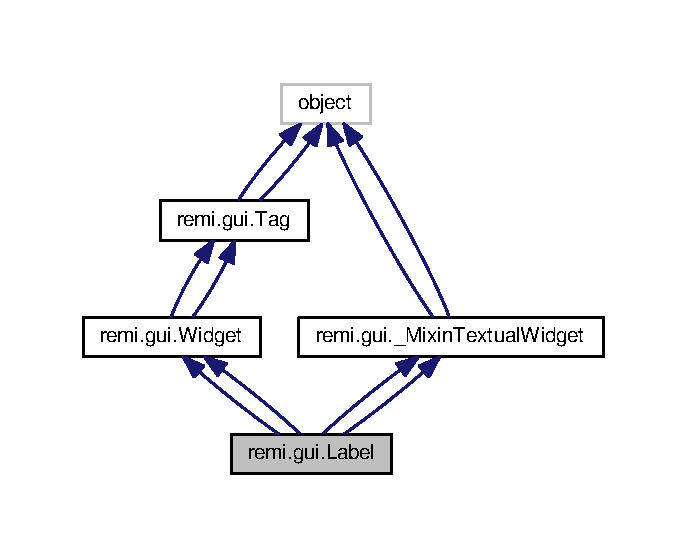
\includegraphics[width=330pt]{d9/d34/classremi_1_1gui_1_1Label__inherit__graph}
\end{center}
\end{figure}


Collaboration diagram for remi.\+gui.\+Label\+:
\nopagebreak
\begin{figure}[H]
\begin{center}
\leavevmode
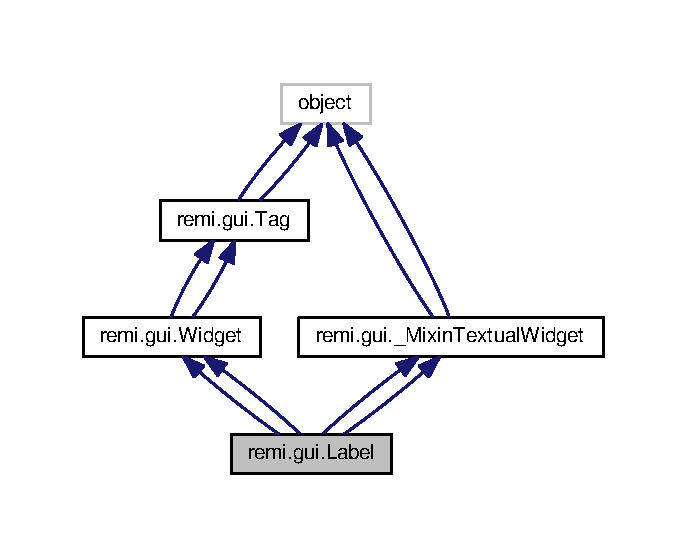
\includegraphics[width=330pt]{de/d4e/classremi_1_1gui_1_1Label__coll__graph}
\end{center}
\end{figure}
\subsection*{Public Member Functions}
\begin{DoxyCompactItemize}
\item 
def \hyperlink{classremi_1_1gui_1_1Label_a277f22b421b7f59cccc7b9e6fc75de9f}{\+\_\+\+\_\+init\+\_\+\+\_\+} (self, text, kwargs)
\item 
def \hyperlink{classremi_1_1gui_1_1Label_a277f22b421b7f59cccc7b9e6fc75de9f}{\+\_\+\+\_\+init\+\_\+\+\_\+} (self, text, kwargs)
\end{DoxyCompactItemize}
\subsection*{Public Attributes}
\begin{DoxyCompactItemize}
\item 
{\bfseries type}\hypertarget{classremi_1_1gui_1_1Label_a987df9e0af9e6b87fb3e0fae6c1e6171}{}\label{classremi_1_1gui_1_1Label_a987df9e0af9e6b87fb3e0fae6c1e6171}

\end{DoxyCompactItemize}
\subsection*{Additional Inherited Members}


\subsection{Detailed Description}
\begin{DoxyVerb}Non editable text label widget. Set its content by means of set_text function, and retrieve its content with the
function get_text.
\end{DoxyVerb}
 

\subsection{Constructor \& Destructor Documentation}
\index{remi\+::gui\+::\+Label@{remi\+::gui\+::\+Label}!\+\_\+\+\_\+init\+\_\+\+\_\+@{\+\_\+\+\_\+init\+\_\+\+\_\+}}
\index{\+\_\+\+\_\+init\+\_\+\+\_\+@{\+\_\+\+\_\+init\+\_\+\+\_\+}!remi\+::gui\+::\+Label@{remi\+::gui\+::\+Label}}
\subsubsection[{\texorpdfstring{\+\_\+\+\_\+init\+\_\+\+\_\+(self, text, kwargs)}{__init__(self, text, kwargs)}}]{\setlength{\rightskip}{0pt plus 5cm}def remi.\+gui.\+Label.\+\_\+\+\_\+init\+\_\+\+\_\+ (
\begin{DoxyParamCaption}
\item[{}]{self, }
\item[{}]{text, }
\item[{}]{kwargs}
\end{DoxyParamCaption}
)}\hypertarget{classremi_1_1gui_1_1Label_a277f22b421b7f59cccc7b9e6fc75de9f}{}\label{classremi_1_1gui_1_1Label_a277f22b421b7f59cccc7b9e6fc75de9f}
\begin{DoxyVerb}Args:
    text (str): The string content that have to be displayed in the Label.
    kwargs: See Widget.__init__()
\end{DoxyVerb}
 \index{remi\+::gui\+::\+Label@{remi\+::gui\+::\+Label}!\+\_\+\+\_\+init\+\_\+\+\_\+@{\+\_\+\+\_\+init\+\_\+\+\_\+}}
\index{\+\_\+\+\_\+init\+\_\+\+\_\+@{\+\_\+\+\_\+init\+\_\+\+\_\+}!remi\+::gui\+::\+Label@{remi\+::gui\+::\+Label}}
\subsubsection[{\texorpdfstring{\+\_\+\+\_\+init\+\_\+\+\_\+(self, text, kwargs)}{__init__(self, text, kwargs)}}]{\setlength{\rightskip}{0pt plus 5cm}def remi.\+gui.\+Label.\+\_\+\+\_\+init\+\_\+\+\_\+ (
\begin{DoxyParamCaption}
\item[{}]{self, }
\item[{}]{text, }
\item[{}]{kwargs}
\end{DoxyParamCaption}
)}\hypertarget{classremi_1_1gui_1_1Label_a277f22b421b7f59cccc7b9e6fc75de9f}{}\label{classremi_1_1gui_1_1Label_a277f22b421b7f59cccc7b9e6fc75de9f}
\begin{DoxyVerb}Args:
    text (str): The string content that have to be displayed in the Label.
    kwargs: See Widget.__init__()
\end{DoxyVerb}
 

The documentation for this class was generated from the following file\+:\begin{DoxyCompactItemize}
\item 
Compiled/\+Server/remi/gui.\+py\end{DoxyCompactItemize}

\hypertarget{classremi_1_1gui_1_1Link}{}\section{remi.\+gui.\+Link Class Reference}
\label{classremi_1_1gui_1_1Link}\index{remi.\+gui.\+Link@{remi.\+gui.\+Link}}


Inheritance diagram for remi.\+gui.\+Link\+:
\nopagebreak
\begin{figure}[H]
\begin{center}
\leavevmode
\includegraphics[width=330pt]{d4/d93/classremi_1_1gui_1_1Link__inherit__graph}
\end{center}
\end{figure}


Collaboration diagram for remi.\+gui.\+Link\+:
\nopagebreak
\begin{figure}[H]
\begin{center}
\leavevmode
\includegraphics[width=330pt]{db/d4e/classremi_1_1gui_1_1Link__coll__graph}
\end{center}
\end{figure}
\subsection*{Public Member Functions}
\begin{DoxyCompactItemize}
\item 
def \hyperlink{classremi_1_1gui_1_1Link_a48356d0197b655fda2b1fd9f4686dbbf}{\+\_\+\+\_\+init\+\_\+\+\_\+} (self, url, text, open\+\_\+new\+\_\+window=True, kwargs)
\item 
def \hyperlink{classremi_1_1gui_1_1Link_acb6497a6b878c0ccdd68acacc1efc9fb}{get\+\_\+url} (self)
\item 
def \hyperlink{classremi_1_1gui_1_1Link_a48356d0197b655fda2b1fd9f4686dbbf}{\+\_\+\+\_\+init\+\_\+\+\_\+} (self, url, text, open\+\_\+new\+\_\+window=True, kwargs)
\item 
def \hyperlink{classremi_1_1gui_1_1Link_acb6497a6b878c0ccdd68acacc1efc9fb}{get\+\_\+url} (self)
\end{DoxyCompactItemize}
\subsection*{Public Attributes}
\begin{DoxyCompactItemize}
\item 
{\bfseries type}\hypertarget{classremi_1_1gui_1_1Link_af76dff7c49ac25c591e17d7024d49e25}{}\label{classremi_1_1gui_1_1Link_af76dff7c49ac25c591e17d7024d49e25}

\end{DoxyCompactItemize}
\subsection*{Additional Inherited Members}


\subsection{Detailed Description}
\begin{DoxyVerb}\end{DoxyVerb}
 

\subsection{Constructor \& Destructor Documentation}
\index{remi\+::gui\+::\+Link@{remi\+::gui\+::\+Link}!\+\_\+\+\_\+init\+\_\+\+\_\+@{\+\_\+\+\_\+init\+\_\+\+\_\+}}
\index{\+\_\+\+\_\+init\+\_\+\+\_\+@{\+\_\+\+\_\+init\+\_\+\+\_\+}!remi\+::gui\+::\+Link@{remi\+::gui\+::\+Link}}
\subsubsection[{\texorpdfstring{\+\_\+\+\_\+init\+\_\+\+\_\+(self, url, text, open\+\_\+new\+\_\+window=\+True, kwargs)}{__init__(self, url, text, open_new_window=True, kwargs)}}]{\setlength{\rightskip}{0pt plus 5cm}def remi.\+gui.\+Link.\+\_\+\+\_\+init\+\_\+\+\_\+ (
\begin{DoxyParamCaption}
\item[{}]{self, }
\item[{}]{url, }
\item[{}]{text, }
\item[{}]{open\+\_\+new\+\_\+window = {\ttfamily True}, }
\item[{}]{kwargs}
\end{DoxyParamCaption}
)}\hypertarget{classremi_1_1gui_1_1Link_a48356d0197b655fda2b1fd9f4686dbbf}{}\label{classremi_1_1gui_1_1Link_a48356d0197b655fda2b1fd9f4686dbbf}
\begin{DoxyVerb}Args:
    url:
    text:
    open_new_window:
    kwargs:
\end{DoxyVerb}
 \index{remi\+::gui\+::\+Link@{remi\+::gui\+::\+Link}!\+\_\+\+\_\+init\+\_\+\+\_\+@{\+\_\+\+\_\+init\+\_\+\+\_\+}}
\index{\+\_\+\+\_\+init\+\_\+\+\_\+@{\+\_\+\+\_\+init\+\_\+\+\_\+}!remi\+::gui\+::\+Link@{remi\+::gui\+::\+Link}}
\subsubsection[{\texorpdfstring{\+\_\+\+\_\+init\+\_\+\+\_\+(self, url, text, open\+\_\+new\+\_\+window=\+True, kwargs)}{__init__(self, url, text, open_new_window=True, kwargs)}}]{\setlength{\rightskip}{0pt plus 5cm}def remi.\+gui.\+Link.\+\_\+\+\_\+init\+\_\+\+\_\+ (
\begin{DoxyParamCaption}
\item[{}]{self, }
\item[{}]{url, }
\item[{}]{text, }
\item[{}]{open\+\_\+new\+\_\+window = {\ttfamily True}, }
\item[{}]{kwargs}
\end{DoxyParamCaption}
)}\hypertarget{classremi_1_1gui_1_1Link_a48356d0197b655fda2b1fd9f4686dbbf}{}\label{classremi_1_1gui_1_1Link_a48356d0197b655fda2b1fd9f4686dbbf}
\begin{DoxyVerb}Args:
    url:
    text:
    open_new_window:
    kwargs:
\end{DoxyVerb}
 

\subsection{Member Function Documentation}
\index{remi\+::gui\+::\+Link@{remi\+::gui\+::\+Link}!get\+\_\+url@{get\+\_\+url}}
\index{get\+\_\+url@{get\+\_\+url}!remi\+::gui\+::\+Link@{remi\+::gui\+::\+Link}}
\subsubsection[{\texorpdfstring{get\+\_\+url(self)}{get_url(self)}}]{\setlength{\rightskip}{0pt plus 5cm}def remi.\+gui.\+Link.\+get\+\_\+url (
\begin{DoxyParamCaption}
\item[{}]{self}
\end{DoxyParamCaption}
)}\hypertarget{classremi_1_1gui_1_1Link_acb6497a6b878c0ccdd68acacc1efc9fb}{}\label{classremi_1_1gui_1_1Link_acb6497a6b878c0ccdd68acacc1efc9fb}
\begin{DoxyVerb}Returns:\end{DoxyVerb}
 \index{remi\+::gui\+::\+Link@{remi\+::gui\+::\+Link}!get\+\_\+url@{get\+\_\+url}}
\index{get\+\_\+url@{get\+\_\+url}!remi\+::gui\+::\+Link@{remi\+::gui\+::\+Link}}
\subsubsection[{\texorpdfstring{get\+\_\+url(self)}{get_url(self)}}]{\setlength{\rightskip}{0pt plus 5cm}def remi.\+gui.\+Link.\+get\+\_\+url (
\begin{DoxyParamCaption}
\item[{}]{self}
\end{DoxyParamCaption}
)}\hypertarget{classremi_1_1gui_1_1Link_acb6497a6b878c0ccdd68acacc1efc9fb}{}\label{classremi_1_1gui_1_1Link_acb6497a6b878c0ccdd68acacc1efc9fb}
\begin{DoxyVerb}Returns:\end{DoxyVerb}
 

The documentation for this class was generated from the following file\+:\begin{DoxyCompactItemize}
\item 
Compiled/\+Server/remi/gui.\+py\end{DoxyCompactItemize}

\hypertarget{classremi_1_1gui_1_1ListItem}{}\section{remi.\+gui.\+List\+Item Class Reference}
\label{classremi_1_1gui_1_1ListItem}\index{remi.\+gui.\+List\+Item@{remi.\+gui.\+List\+Item}}


Inheritance diagram for remi.\+gui.\+List\+Item\+:
\nopagebreak
\begin{figure}[H]
\begin{center}
\leavevmode
\includegraphics[width=330pt]{d5/d64/classremi_1_1gui_1_1ListItem__inherit__graph}
\end{center}
\end{figure}


Collaboration diagram for remi.\+gui.\+List\+Item\+:
\nopagebreak
\begin{figure}[H]
\begin{center}
\leavevmode
\includegraphics[width=330pt]{d0/d5e/classremi_1_1gui_1_1ListItem__coll__graph}
\end{center}
\end{figure}
\subsection*{Public Member Functions}
\begin{DoxyCompactItemize}
\item 
def \hyperlink{classremi_1_1gui_1_1ListItem_af778922b9d51e37a3f7bf98aa93ecc54}{\+\_\+\+\_\+init\+\_\+\+\_\+} (self, text, kwargs)
\item 
def \hyperlink{classremi_1_1gui_1_1ListItem_ab2dff2b03f6c88f3caebea53481db957}{get\+\_\+value} (self)
\item 
def \hyperlink{classremi_1_1gui_1_1ListItem_ae04f42afb8aeaba38d602912d2fc4736}{onclick} (self)
\item 
def \hyperlink{classremi_1_1gui_1_1ListItem_af778922b9d51e37a3f7bf98aa93ecc54}{\+\_\+\+\_\+init\+\_\+\+\_\+} (self, text, kwargs)
\item 
def \hyperlink{classremi_1_1gui_1_1ListItem_ab2dff2b03f6c88f3caebea53481db957}{get\+\_\+value} (self)
\item 
def \hyperlink{classremi_1_1gui_1_1ListItem_ae04f42afb8aeaba38d602912d2fc4736}{onclick} (self)
\end{DoxyCompactItemize}
\subsection*{Public Attributes}
\begin{DoxyCompactItemize}
\item 
{\bfseries type}\hypertarget{classremi_1_1gui_1_1ListItem_acb0badfd2f0d808c4902cc73d1d3c158}{}\label{classremi_1_1gui_1_1ListItem_acb0badfd2f0d808c4902cc73d1d3c158}

\end{DoxyCompactItemize}
\subsection*{Additional Inherited Members}


\subsection{Detailed Description}
\begin{DoxyVerb}List item widget for the ListView.

ListItems are characterized by a textual content. They can be selected from
the ListView. Do NOT manage directly its selection by registering set_on_click_listener, use instead the events of
the ListView.
\end{DoxyVerb}
 

\subsection{Constructor \& Destructor Documentation}
\index{remi\+::gui\+::\+List\+Item@{remi\+::gui\+::\+List\+Item}!\+\_\+\+\_\+init\+\_\+\+\_\+@{\+\_\+\+\_\+init\+\_\+\+\_\+}}
\index{\+\_\+\+\_\+init\+\_\+\+\_\+@{\+\_\+\+\_\+init\+\_\+\+\_\+}!remi\+::gui\+::\+List\+Item@{remi\+::gui\+::\+List\+Item}}
\subsubsection[{\texorpdfstring{\+\_\+\+\_\+init\+\_\+\+\_\+(self, text, kwargs)}{__init__(self, text, kwargs)}}]{\setlength{\rightskip}{0pt plus 5cm}def remi.\+gui.\+List\+Item.\+\_\+\+\_\+init\+\_\+\+\_\+ (
\begin{DoxyParamCaption}
\item[{}]{self, }
\item[{}]{text, }
\item[{}]{kwargs}
\end{DoxyParamCaption}
)}\hypertarget{classremi_1_1gui_1_1ListItem_af778922b9d51e37a3f7bf98aa93ecc54}{}\label{classremi_1_1gui_1_1ListItem_af778922b9d51e37a3f7bf98aa93ecc54}
\begin{DoxyVerb}Args:
    text (str, unicode): The textual content of the ListItem.
    kwargs: See Widget.__init__()
\end{DoxyVerb}
 \index{remi\+::gui\+::\+List\+Item@{remi\+::gui\+::\+List\+Item}!\+\_\+\+\_\+init\+\_\+\+\_\+@{\+\_\+\+\_\+init\+\_\+\+\_\+}}
\index{\+\_\+\+\_\+init\+\_\+\+\_\+@{\+\_\+\+\_\+init\+\_\+\+\_\+}!remi\+::gui\+::\+List\+Item@{remi\+::gui\+::\+List\+Item}}
\subsubsection[{\texorpdfstring{\+\_\+\+\_\+init\+\_\+\+\_\+(self, text, kwargs)}{__init__(self, text, kwargs)}}]{\setlength{\rightskip}{0pt plus 5cm}def remi.\+gui.\+List\+Item.\+\_\+\+\_\+init\+\_\+\+\_\+ (
\begin{DoxyParamCaption}
\item[{}]{self, }
\item[{}]{text, }
\item[{}]{kwargs}
\end{DoxyParamCaption}
)}\hypertarget{classremi_1_1gui_1_1ListItem_af778922b9d51e37a3f7bf98aa93ecc54}{}\label{classremi_1_1gui_1_1ListItem_af778922b9d51e37a3f7bf98aa93ecc54}
\begin{DoxyVerb}Args:
    text (str, unicode): The textual content of the ListItem.
    kwargs: See Widget.__init__()
\end{DoxyVerb}
 

\subsection{Member Function Documentation}
\index{remi\+::gui\+::\+List\+Item@{remi\+::gui\+::\+List\+Item}!get\+\_\+value@{get\+\_\+value}}
\index{get\+\_\+value@{get\+\_\+value}!remi\+::gui\+::\+List\+Item@{remi\+::gui\+::\+List\+Item}}
\subsubsection[{\texorpdfstring{get\+\_\+value(self)}{get_value(self)}}]{\setlength{\rightskip}{0pt plus 5cm}def remi.\+gui.\+List\+Item.\+get\+\_\+value (
\begin{DoxyParamCaption}
\item[{}]{self}
\end{DoxyParamCaption}
)}\hypertarget{classremi_1_1gui_1_1ListItem_ab2dff2b03f6c88f3caebea53481db957}{}\label{classremi_1_1gui_1_1ListItem_ab2dff2b03f6c88f3caebea53481db957}
\begin{DoxyVerb}Returns:
    str: The text content of the ListItem
\end{DoxyVerb}
 \index{remi\+::gui\+::\+List\+Item@{remi\+::gui\+::\+List\+Item}!get\+\_\+value@{get\+\_\+value}}
\index{get\+\_\+value@{get\+\_\+value}!remi\+::gui\+::\+List\+Item@{remi\+::gui\+::\+List\+Item}}
\subsubsection[{\texorpdfstring{get\+\_\+value(self)}{get_value(self)}}]{\setlength{\rightskip}{0pt plus 5cm}def remi.\+gui.\+List\+Item.\+get\+\_\+value (
\begin{DoxyParamCaption}
\item[{}]{self}
\end{DoxyParamCaption}
)}\hypertarget{classremi_1_1gui_1_1ListItem_ab2dff2b03f6c88f3caebea53481db957}{}\label{classremi_1_1gui_1_1ListItem_ab2dff2b03f6c88f3caebea53481db957}
\begin{DoxyVerb}Returns:
    str: The text content of the ListItem
\end{DoxyVerb}
 \index{remi\+::gui\+::\+List\+Item@{remi\+::gui\+::\+List\+Item}!onclick@{onclick}}
\index{onclick@{onclick}!remi\+::gui\+::\+List\+Item@{remi\+::gui\+::\+List\+Item}}
\subsubsection[{\texorpdfstring{onclick(self)}{onclick(self)}}]{\setlength{\rightskip}{0pt plus 5cm}def remi.\+gui.\+List\+Item.\+onclick (
\begin{DoxyParamCaption}
\item[{}]{self}
\end{DoxyParamCaption}
)}\hypertarget{classremi_1_1gui_1_1ListItem_ae04f42afb8aeaba38d602912d2fc4736}{}\label{classremi_1_1gui_1_1ListItem_ae04f42afb8aeaba38d602912d2fc4736}
\begin{DoxyVerb}Called when the item gets clicked. It is managed by the container ListView.\end{DoxyVerb}
 \index{remi\+::gui\+::\+List\+Item@{remi\+::gui\+::\+List\+Item}!onclick@{onclick}}
\index{onclick@{onclick}!remi\+::gui\+::\+List\+Item@{remi\+::gui\+::\+List\+Item}}
\subsubsection[{\texorpdfstring{onclick(self)}{onclick(self)}}]{\setlength{\rightskip}{0pt plus 5cm}def remi.\+gui.\+List\+Item.\+onclick (
\begin{DoxyParamCaption}
\item[{}]{self}
\end{DoxyParamCaption}
)}\hypertarget{classremi_1_1gui_1_1ListItem_ae04f42afb8aeaba38d602912d2fc4736}{}\label{classremi_1_1gui_1_1ListItem_ae04f42afb8aeaba38d602912d2fc4736}
\begin{DoxyVerb}Called when the item gets clicked. It is managed by the container ListView.\end{DoxyVerb}
 

The documentation for this class was generated from the following file\+:\begin{DoxyCompactItemize}
\item 
Compiled/\+Server/remi/gui.\+py\end{DoxyCompactItemize}

\hypertarget{classremi_1_1gui_1_1ListView}{}\section{remi.\+gui.\+List\+View Class Reference}
\label{classremi_1_1gui_1_1ListView}\index{remi.\+gui.\+List\+View@{remi.\+gui.\+List\+View}}


Inheritance diagram for remi.\+gui.\+List\+View\+:
\nopagebreak
\begin{figure}[H]
\begin{center}
\leavevmode
\includegraphics[width=314pt]{d3/de5/classremi_1_1gui_1_1ListView__inherit__graph}
\end{center}
\end{figure}


Collaboration diagram for remi.\+gui.\+List\+View\+:
\nopagebreak
\begin{figure}[H]
\begin{center}
\leavevmode
\includegraphics[width=314pt]{d6/d2b/classremi_1_1gui_1_1ListView__coll__graph}
\end{center}
\end{figure}
\subsection*{Public Member Functions}
\begin{DoxyCompactItemize}
\item 
def \hyperlink{classremi_1_1gui_1_1ListView_a0d33a469484fe97d78e7122ee04dd8e7}{\+\_\+\+\_\+init\+\_\+\+\_\+} (self, selectable=True, kwargs)
\item 
def \hyperlink{classremi_1_1gui_1_1ListView_aaf113567a3811e687eee0a7b70d49f95}{new\+\_\+from\+\_\+list} (cls, items, kwargs)
\item 
def \hyperlink{classremi_1_1gui_1_1ListView_af7deb210e778936cd09bc665de7ada81}{append} (self, item, key=\textquotesingle{}\textquotesingle{})
\item 
def \hyperlink{classremi_1_1gui_1_1ListView_a8142a456f56465229168e7910b2a5406}{empty} (self)
\item 
def \hyperlink{classremi_1_1gui_1_1ListView_adcdc5be097dc81ce9e96b36adeb63d1c}{onselection} (self, widget)
\item 
def \hyperlink{classremi_1_1gui_1_1ListView_aae509720cebc82534989b955bcbc82c8}{set\+\_\+on\+\_\+selection\+\_\+listener} (self, callback, userdata)
\item 
def \hyperlink{classremi_1_1gui_1_1ListView_ad729d9dc0f1e6fd8c42e3f0205c0efc7}{get\+\_\+value} (self)
\item 
def \hyperlink{classremi_1_1gui_1_1ListView_ae916dd25166229d79ed619bf51bfad10}{get\+\_\+key} (self)
\item 
def \hyperlink{classremi_1_1gui_1_1ListView_aedfdc65ab96226786f68bbab0d1c1eec}{select\+\_\+by\+\_\+key} (self, key)
\item 
def \hyperlink{classremi_1_1gui_1_1ListView_a2691e177503dde04d12b1312b597a9ec}{set\+\_\+value} (self, value)
\item 
def \hyperlink{classremi_1_1gui_1_1ListView_a9be5a47ec5d98915429a3486b8611f1f}{select\+\_\+by\+\_\+value} (self, value)
\item 
def \hyperlink{classremi_1_1gui_1_1ListView_a0d33a469484fe97d78e7122ee04dd8e7}{\+\_\+\+\_\+init\+\_\+\+\_\+} (self, selectable=True, kwargs)
\item 
def \hyperlink{classremi_1_1gui_1_1ListView_aaf113567a3811e687eee0a7b70d49f95}{new\+\_\+from\+\_\+list} (cls, items, kwargs)
\item 
def \hyperlink{classremi_1_1gui_1_1ListView_af7deb210e778936cd09bc665de7ada81}{append} (self, item, key=\textquotesingle{}\textquotesingle{})
\item 
def \hyperlink{classremi_1_1gui_1_1ListView_a8142a456f56465229168e7910b2a5406}{empty} (self)
\item 
def \hyperlink{classremi_1_1gui_1_1ListView_adcdc5be097dc81ce9e96b36adeb63d1c}{onselection} (self, widget)
\item 
def \hyperlink{classremi_1_1gui_1_1ListView_aae509720cebc82534989b955bcbc82c8}{set\+\_\+on\+\_\+selection\+\_\+listener} (self, callback, userdata)
\item 
def \hyperlink{classremi_1_1gui_1_1ListView_ad729d9dc0f1e6fd8c42e3f0205c0efc7}{get\+\_\+value} (self)
\item 
def \hyperlink{classremi_1_1gui_1_1ListView_ae916dd25166229d79ed619bf51bfad10}{get\+\_\+key} (self)
\item 
def \hyperlink{classremi_1_1gui_1_1ListView_aedfdc65ab96226786f68bbab0d1c1eec}{select\+\_\+by\+\_\+key} (self, key)
\item 
def \hyperlink{classremi_1_1gui_1_1ListView_a2691e177503dde04d12b1312b597a9ec}{set\+\_\+value} (self, value)
\item 
def \hyperlink{classremi_1_1gui_1_1ListView_a9be5a47ec5d98915429a3486b8611f1f}{select\+\_\+by\+\_\+value} (self, value)
\end{DoxyCompactItemize}
\subsection*{Public Attributes}
\begin{DoxyCompactItemize}
\item 
{\bfseries type}\hypertarget{classremi_1_1gui_1_1ListView_a8a6331d3580fdb495af3f808aa92cdab}{}\label{classremi_1_1gui_1_1ListView_a8a6331d3580fdb495af3f808aa92cdab}

\end{DoxyCompactItemize}
\subsection*{Static Public Attributes}
\begin{DoxyCompactItemize}
\item 
string {\bfseries E\+V\+E\+N\+T\+\_\+\+O\+N\+S\+E\+L\+E\+C\+T\+I\+ON} = \textquotesingle{}\hyperlink{classremi_1_1gui_1_1ListView_adcdc5be097dc81ce9e96b36adeb63d1c}{onselection}\textquotesingle{}\hypertarget{classremi_1_1gui_1_1ListView_a88da212b5bf6284eef0cf0887e8dc9a8}{}\label{classremi_1_1gui_1_1ListView_a88da212b5bf6284eef0cf0887e8dc9a8}

\end{DoxyCompactItemize}


\subsection{Detailed Description}
\begin{DoxyVerb}List widget it can contain ListItems. Add items to it by using the standard append(item, key) function or
generate a filled list from a string list by means of the function new_from_list. Use the list in conjunction of
its onselection event. Register a listener with ListView.set_on_selection_listener.
\end{DoxyVerb}
 

\subsection{Constructor \& Destructor Documentation}
\index{remi\+::gui\+::\+List\+View@{remi\+::gui\+::\+List\+View}!\+\_\+\+\_\+init\+\_\+\+\_\+@{\+\_\+\+\_\+init\+\_\+\+\_\+}}
\index{\+\_\+\+\_\+init\+\_\+\+\_\+@{\+\_\+\+\_\+init\+\_\+\+\_\+}!remi\+::gui\+::\+List\+View@{remi\+::gui\+::\+List\+View}}
\subsubsection[{\texorpdfstring{\+\_\+\+\_\+init\+\_\+\+\_\+(self, selectable=\+True, kwargs)}{__init__(self, selectable=True, kwargs)}}]{\setlength{\rightskip}{0pt plus 5cm}def remi.\+gui.\+List\+View.\+\_\+\+\_\+init\+\_\+\+\_\+ (
\begin{DoxyParamCaption}
\item[{}]{self, }
\item[{}]{selectable = {\ttfamily True}, }
\item[{}]{kwargs}
\end{DoxyParamCaption}
)}\hypertarget{classremi_1_1gui_1_1ListView_a0d33a469484fe97d78e7122ee04dd8e7}{}\label{classremi_1_1gui_1_1ListView_a0d33a469484fe97d78e7122ee04dd8e7}
\begin{DoxyVerb}Args:
    kwargs: See Widget.__init__()
\end{DoxyVerb}
 \index{remi\+::gui\+::\+List\+View@{remi\+::gui\+::\+List\+View}!\+\_\+\+\_\+init\+\_\+\+\_\+@{\+\_\+\+\_\+init\+\_\+\+\_\+}}
\index{\+\_\+\+\_\+init\+\_\+\+\_\+@{\+\_\+\+\_\+init\+\_\+\+\_\+}!remi\+::gui\+::\+List\+View@{remi\+::gui\+::\+List\+View}}
\subsubsection[{\texorpdfstring{\+\_\+\+\_\+init\+\_\+\+\_\+(self, selectable=\+True, kwargs)}{__init__(self, selectable=True, kwargs)}}]{\setlength{\rightskip}{0pt plus 5cm}def remi.\+gui.\+List\+View.\+\_\+\+\_\+init\+\_\+\+\_\+ (
\begin{DoxyParamCaption}
\item[{}]{self, }
\item[{}]{selectable = {\ttfamily True}, }
\item[{}]{kwargs}
\end{DoxyParamCaption}
)}\hypertarget{classremi_1_1gui_1_1ListView_a0d33a469484fe97d78e7122ee04dd8e7}{}\label{classremi_1_1gui_1_1ListView_a0d33a469484fe97d78e7122ee04dd8e7}
\begin{DoxyVerb}Args:
    kwargs: See Widget.__init__()
\end{DoxyVerb}
 

\subsection{Member Function Documentation}
\index{remi\+::gui\+::\+List\+View@{remi\+::gui\+::\+List\+View}!append@{append}}
\index{append@{append}!remi\+::gui\+::\+List\+View@{remi\+::gui\+::\+List\+View}}
\subsubsection[{\texorpdfstring{append(self, item, key=\textquotesingle{}\textquotesingle{})}{append(self, item, key='')}}]{\setlength{\rightskip}{0pt plus 5cm}def remi.\+gui.\+List\+View.\+append (
\begin{DoxyParamCaption}
\item[{}]{self, }
\item[{}]{item, }
\item[{}]{key = {\ttfamily \textquotesingle{}\textquotesingle{}}}
\end{DoxyParamCaption}
)}\hypertarget{classremi_1_1gui_1_1ListView_af7deb210e778936cd09bc665de7ada81}{}\label{classremi_1_1gui_1_1ListView_af7deb210e778936cd09bc665de7ada81}
\begin{DoxyVerb}Appends child items to the ListView. The items are accessible by list.children[key].

Args:
    item (ListItem): the item to add.
    key (str): string key for the item.
\end{DoxyVerb}
 \index{remi\+::gui\+::\+List\+View@{remi\+::gui\+::\+List\+View}!append@{append}}
\index{append@{append}!remi\+::gui\+::\+List\+View@{remi\+::gui\+::\+List\+View}}
\subsubsection[{\texorpdfstring{append(self, item, key=\textquotesingle{}\textquotesingle{})}{append(self, item, key='')}}]{\setlength{\rightskip}{0pt plus 5cm}def remi.\+gui.\+List\+View.\+append (
\begin{DoxyParamCaption}
\item[{}]{self, }
\item[{}]{item, }
\item[{}]{key = {\ttfamily \textquotesingle{}\textquotesingle{}}}
\end{DoxyParamCaption}
)}\hypertarget{classremi_1_1gui_1_1ListView_af7deb210e778936cd09bc665de7ada81}{}\label{classremi_1_1gui_1_1ListView_af7deb210e778936cd09bc665de7ada81}
\begin{DoxyVerb}Appends child items to the ListView. The items are accessible by list.children[key].

Args:
    item (ListItem): the item to add.
    key (str): string key for the item.
\end{DoxyVerb}
 \index{remi\+::gui\+::\+List\+View@{remi\+::gui\+::\+List\+View}!empty@{empty}}
\index{empty@{empty}!remi\+::gui\+::\+List\+View@{remi\+::gui\+::\+List\+View}}
\subsubsection[{\texorpdfstring{empty(self)}{empty(self)}}]{\setlength{\rightskip}{0pt plus 5cm}def remi.\+gui.\+List\+View.\+empty (
\begin{DoxyParamCaption}
\item[{}]{self}
\end{DoxyParamCaption}
)}\hypertarget{classremi_1_1gui_1_1ListView_a8142a456f56465229168e7910b2a5406}{}\label{classremi_1_1gui_1_1ListView_a8142a456f56465229168e7910b2a5406}
\begin{DoxyVerb}Removes all children from the list\end{DoxyVerb}
 \index{remi\+::gui\+::\+List\+View@{remi\+::gui\+::\+List\+View}!empty@{empty}}
\index{empty@{empty}!remi\+::gui\+::\+List\+View@{remi\+::gui\+::\+List\+View}}
\subsubsection[{\texorpdfstring{empty(self)}{empty(self)}}]{\setlength{\rightskip}{0pt plus 5cm}def remi.\+gui.\+List\+View.\+empty (
\begin{DoxyParamCaption}
\item[{}]{self}
\end{DoxyParamCaption}
)}\hypertarget{classremi_1_1gui_1_1ListView_a8142a456f56465229168e7910b2a5406}{}\label{classremi_1_1gui_1_1ListView_a8142a456f56465229168e7910b2a5406}
\begin{DoxyVerb}Removes all children from the list\end{DoxyVerb}
 \index{remi\+::gui\+::\+List\+View@{remi\+::gui\+::\+List\+View}!get\+\_\+key@{get\+\_\+key}}
\index{get\+\_\+key@{get\+\_\+key}!remi\+::gui\+::\+List\+View@{remi\+::gui\+::\+List\+View}}
\subsubsection[{\texorpdfstring{get\+\_\+key(self)}{get_key(self)}}]{\setlength{\rightskip}{0pt plus 5cm}def remi.\+gui.\+List\+View.\+get\+\_\+key (
\begin{DoxyParamCaption}
\item[{}]{self}
\end{DoxyParamCaption}
)}\hypertarget{classremi_1_1gui_1_1ListView_ae916dd25166229d79ed619bf51bfad10}{}\label{classremi_1_1gui_1_1ListView_ae916dd25166229d79ed619bf51bfad10}
\begin{DoxyVerb}Returns:
    str: The key of the selected item or None if no item is selected.
\end{DoxyVerb}
 \index{remi\+::gui\+::\+List\+View@{remi\+::gui\+::\+List\+View}!get\+\_\+key@{get\+\_\+key}}
\index{get\+\_\+key@{get\+\_\+key}!remi\+::gui\+::\+List\+View@{remi\+::gui\+::\+List\+View}}
\subsubsection[{\texorpdfstring{get\+\_\+key(self)}{get_key(self)}}]{\setlength{\rightskip}{0pt plus 5cm}def remi.\+gui.\+List\+View.\+get\+\_\+key (
\begin{DoxyParamCaption}
\item[{}]{self}
\end{DoxyParamCaption}
)}\hypertarget{classremi_1_1gui_1_1ListView_ae916dd25166229d79ed619bf51bfad10}{}\label{classremi_1_1gui_1_1ListView_ae916dd25166229d79ed619bf51bfad10}
\begin{DoxyVerb}Returns:
    str: The key of the selected item or None if no item is selected.
\end{DoxyVerb}
 \index{remi\+::gui\+::\+List\+View@{remi\+::gui\+::\+List\+View}!get\+\_\+value@{get\+\_\+value}}
\index{get\+\_\+value@{get\+\_\+value}!remi\+::gui\+::\+List\+View@{remi\+::gui\+::\+List\+View}}
\subsubsection[{\texorpdfstring{get\+\_\+value(self)}{get_value(self)}}]{\setlength{\rightskip}{0pt plus 5cm}def remi.\+gui.\+List\+View.\+get\+\_\+value (
\begin{DoxyParamCaption}
\item[{}]{self}
\end{DoxyParamCaption}
)}\hypertarget{classremi_1_1gui_1_1ListView_ad729d9dc0f1e6fd8c42e3f0205c0efc7}{}\label{classremi_1_1gui_1_1ListView_ad729d9dc0f1e6fd8c42e3f0205c0efc7}
\begin{DoxyVerb}Returns:
    str: The value of the selected item or None
\end{DoxyVerb}
 \index{remi\+::gui\+::\+List\+View@{remi\+::gui\+::\+List\+View}!get\+\_\+value@{get\+\_\+value}}
\index{get\+\_\+value@{get\+\_\+value}!remi\+::gui\+::\+List\+View@{remi\+::gui\+::\+List\+View}}
\subsubsection[{\texorpdfstring{get\+\_\+value(self)}{get_value(self)}}]{\setlength{\rightskip}{0pt plus 5cm}def remi.\+gui.\+List\+View.\+get\+\_\+value (
\begin{DoxyParamCaption}
\item[{}]{self}
\end{DoxyParamCaption}
)}\hypertarget{classremi_1_1gui_1_1ListView_ad729d9dc0f1e6fd8c42e3f0205c0efc7}{}\label{classremi_1_1gui_1_1ListView_ad729d9dc0f1e6fd8c42e3f0205c0efc7}
\begin{DoxyVerb}Returns:
    str: The value of the selected item or None
\end{DoxyVerb}
 \index{remi\+::gui\+::\+List\+View@{remi\+::gui\+::\+List\+View}!new\+\_\+from\+\_\+list@{new\+\_\+from\+\_\+list}}
\index{new\+\_\+from\+\_\+list@{new\+\_\+from\+\_\+list}!remi\+::gui\+::\+List\+View@{remi\+::gui\+::\+List\+View}}
\subsubsection[{\texorpdfstring{new\+\_\+from\+\_\+list(cls, items, kwargs)}{new_from_list(cls, items, kwargs)}}]{\setlength{\rightskip}{0pt plus 5cm}def remi.\+gui.\+List\+View.\+new\+\_\+from\+\_\+list (
\begin{DoxyParamCaption}
\item[{}]{cls, }
\item[{}]{items, }
\item[{}]{kwargs}
\end{DoxyParamCaption}
)}\hypertarget{classremi_1_1gui_1_1ListView_aaf113567a3811e687eee0a7b70d49f95}{}\label{classremi_1_1gui_1_1ListView_aaf113567a3811e687eee0a7b70d49f95}
\begin{DoxyVerb}Populates the ListView with a string list.

Args:
    items (list): list of strings to fill the widget with.
\end{DoxyVerb}
 \index{remi\+::gui\+::\+List\+View@{remi\+::gui\+::\+List\+View}!new\+\_\+from\+\_\+list@{new\+\_\+from\+\_\+list}}
\index{new\+\_\+from\+\_\+list@{new\+\_\+from\+\_\+list}!remi\+::gui\+::\+List\+View@{remi\+::gui\+::\+List\+View}}
\subsubsection[{\texorpdfstring{new\+\_\+from\+\_\+list(cls, items, kwargs)}{new_from_list(cls, items, kwargs)}}]{\setlength{\rightskip}{0pt plus 5cm}def remi.\+gui.\+List\+View.\+new\+\_\+from\+\_\+list (
\begin{DoxyParamCaption}
\item[{}]{cls, }
\item[{}]{items, }
\item[{}]{kwargs}
\end{DoxyParamCaption}
)}\hypertarget{classremi_1_1gui_1_1ListView_aaf113567a3811e687eee0a7b70d49f95}{}\label{classremi_1_1gui_1_1ListView_aaf113567a3811e687eee0a7b70d49f95}
\begin{DoxyVerb}Populates the ListView with a string list.

Args:
    items (list): list of strings to fill the widget with.
\end{DoxyVerb}
 \index{remi\+::gui\+::\+List\+View@{remi\+::gui\+::\+List\+View}!onselection@{onselection}}
\index{onselection@{onselection}!remi\+::gui\+::\+List\+View@{remi\+::gui\+::\+List\+View}}
\subsubsection[{\texorpdfstring{onselection(self, widget)}{onselection(self, widget)}}]{\setlength{\rightskip}{0pt plus 5cm}def remi.\+gui.\+List\+View.\+onselection (
\begin{DoxyParamCaption}
\item[{}]{self, }
\item[{}]{widget}
\end{DoxyParamCaption}
)}\hypertarget{classremi_1_1gui_1_1ListView_adcdc5be097dc81ce9e96b36adeb63d1c}{}\label{classremi_1_1gui_1_1ListView_adcdc5be097dc81ce9e96b36adeb63d1c}
\begin{DoxyVerb}Called when a new item gets selected in the list.\end{DoxyVerb}
 \index{remi\+::gui\+::\+List\+View@{remi\+::gui\+::\+List\+View}!onselection@{onselection}}
\index{onselection@{onselection}!remi\+::gui\+::\+List\+View@{remi\+::gui\+::\+List\+View}}
\subsubsection[{\texorpdfstring{onselection(self, widget)}{onselection(self, widget)}}]{\setlength{\rightskip}{0pt plus 5cm}def remi.\+gui.\+List\+View.\+onselection (
\begin{DoxyParamCaption}
\item[{}]{self, }
\item[{}]{widget}
\end{DoxyParamCaption}
)}\hypertarget{classremi_1_1gui_1_1ListView_adcdc5be097dc81ce9e96b36adeb63d1c}{}\label{classremi_1_1gui_1_1ListView_adcdc5be097dc81ce9e96b36adeb63d1c}
\begin{DoxyVerb}Called when a new item gets selected in the list.\end{DoxyVerb}
 \index{remi\+::gui\+::\+List\+View@{remi\+::gui\+::\+List\+View}!select\+\_\+by\+\_\+key@{select\+\_\+by\+\_\+key}}
\index{select\+\_\+by\+\_\+key@{select\+\_\+by\+\_\+key}!remi\+::gui\+::\+List\+View@{remi\+::gui\+::\+List\+View}}
\subsubsection[{\texorpdfstring{select\+\_\+by\+\_\+key(self, key)}{select_by_key(self, key)}}]{\setlength{\rightskip}{0pt plus 5cm}def remi.\+gui.\+List\+View.\+select\+\_\+by\+\_\+key (
\begin{DoxyParamCaption}
\item[{}]{self, }
\item[{}]{key}
\end{DoxyParamCaption}
)}\hypertarget{classremi_1_1gui_1_1ListView_aedfdc65ab96226786f68bbab0d1c1eec}{}\label{classremi_1_1gui_1_1ListView_aedfdc65ab96226786f68bbab0d1c1eec}
\begin{DoxyVerb}Selects an item by its key.

Args:
    key (str): The unique string identifier of the item that have to be selected.
\end{DoxyVerb}
 \index{remi\+::gui\+::\+List\+View@{remi\+::gui\+::\+List\+View}!select\+\_\+by\+\_\+key@{select\+\_\+by\+\_\+key}}
\index{select\+\_\+by\+\_\+key@{select\+\_\+by\+\_\+key}!remi\+::gui\+::\+List\+View@{remi\+::gui\+::\+List\+View}}
\subsubsection[{\texorpdfstring{select\+\_\+by\+\_\+key(self, key)}{select_by_key(self, key)}}]{\setlength{\rightskip}{0pt plus 5cm}def remi.\+gui.\+List\+View.\+select\+\_\+by\+\_\+key (
\begin{DoxyParamCaption}
\item[{}]{self, }
\item[{}]{key}
\end{DoxyParamCaption}
)}\hypertarget{classremi_1_1gui_1_1ListView_aedfdc65ab96226786f68bbab0d1c1eec}{}\label{classremi_1_1gui_1_1ListView_aedfdc65ab96226786f68bbab0d1c1eec}
\begin{DoxyVerb}Selects an item by its key.

Args:
    key (str): The unique string identifier of the item that have to be selected.
\end{DoxyVerb}
 \index{remi\+::gui\+::\+List\+View@{remi\+::gui\+::\+List\+View}!select\+\_\+by\+\_\+value@{select\+\_\+by\+\_\+value}}
\index{select\+\_\+by\+\_\+value@{select\+\_\+by\+\_\+value}!remi\+::gui\+::\+List\+View@{remi\+::gui\+::\+List\+View}}
\subsubsection[{\texorpdfstring{select\+\_\+by\+\_\+value(self, value)}{select_by_value(self, value)}}]{\setlength{\rightskip}{0pt plus 5cm}def remi.\+gui.\+List\+View.\+select\+\_\+by\+\_\+value (
\begin{DoxyParamCaption}
\item[{}]{self, }
\item[{}]{value}
\end{DoxyParamCaption}
)}\hypertarget{classremi_1_1gui_1_1ListView_a9be5a47ec5d98915429a3486b8611f1f}{}\label{classremi_1_1gui_1_1ListView_a9be5a47ec5d98915429a3486b8611f1f}
\begin{DoxyVerb}Selects an item by the text content of the child.

Args:
    value (str): Text content of the item that have to be selected.
\end{DoxyVerb}
 \index{remi\+::gui\+::\+List\+View@{remi\+::gui\+::\+List\+View}!select\+\_\+by\+\_\+value@{select\+\_\+by\+\_\+value}}
\index{select\+\_\+by\+\_\+value@{select\+\_\+by\+\_\+value}!remi\+::gui\+::\+List\+View@{remi\+::gui\+::\+List\+View}}
\subsubsection[{\texorpdfstring{select\+\_\+by\+\_\+value(self, value)}{select_by_value(self, value)}}]{\setlength{\rightskip}{0pt plus 5cm}def remi.\+gui.\+List\+View.\+select\+\_\+by\+\_\+value (
\begin{DoxyParamCaption}
\item[{}]{self, }
\item[{}]{value}
\end{DoxyParamCaption}
)}\hypertarget{classremi_1_1gui_1_1ListView_a9be5a47ec5d98915429a3486b8611f1f}{}\label{classremi_1_1gui_1_1ListView_a9be5a47ec5d98915429a3486b8611f1f}
\begin{DoxyVerb}Selects an item by the text content of the child.

Args:
    value (str): Text content of the item that have to be selected.
\end{DoxyVerb}
 \index{remi\+::gui\+::\+List\+View@{remi\+::gui\+::\+List\+View}!set\+\_\+on\+\_\+selection\+\_\+listener@{set\+\_\+on\+\_\+selection\+\_\+listener}}
\index{set\+\_\+on\+\_\+selection\+\_\+listener@{set\+\_\+on\+\_\+selection\+\_\+listener}!remi\+::gui\+::\+List\+View@{remi\+::gui\+::\+List\+View}}
\subsubsection[{\texorpdfstring{set\+\_\+on\+\_\+selection\+\_\+listener(self, callback, userdata)}{set_on_selection_listener(self, callback, userdata)}}]{\setlength{\rightskip}{0pt plus 5cm}def remi.\+gui.\+List\+View.\+set\+\_\+on\+\_\+selection\+\_\+listener (
\begin{DoxyParamCaption}
\item[{}]{self, }
\item[{}]{callback, }
\item[{}]{userdata}
\end{DoxyParamCaption}
)}\hypertarget{classremi_1_1gui_1_1ListView_aae509720cebc82534989b955bcbc82c8}{}\label{classremi_1_1gui_1_1ListView_aae509720cebc82534989b955bcbc82c8}
\begin{DoxyVerb}Registers the listener for the ListView.onselection event.

Note: The prototype of the listener have to be like my_list_onselection(self, widget, selectedKey). Where
selectedKey is the unique string identifier for the selected item. To access the item use
ListView.children[key], or its value directly by ListView.get_value.

Args:
    callback (function): Callback function pointer.
\end{DoxyVerb}
 \index{remi\+::gui\+::\+List\+View@{remi\+::gui\+::\+List\+View}!set\+\_\+on\+\_\+selection\+\_\+listener@{set\+\_\+on\+\_\+selection\+\_\+listener}}
\index{set\+\_\+on\+\_\+selection\+\_\+listener@{set\+\_\+on\+\_\+selection\+\_\+listener}!remi\+::gui\+::\+List\+View@{remi\+::gui\+::\+List\+View}}
\subsubsection[{\texorpdfstring{set\+\_\+on\+\_\+selection\+\_\+listener(self, callback, userdata)}{set_on_selection_listener(self, callback, userdata)}}]{\setlength{\rightskip}{0pt plus 5cm}def remi.\+gui.\+List\+View.\+set\+\_\+on\+\_\+selection\+\_\+listener (
\begin{DoxyParamCaption}
\item[{}]{self, }
\item[{}]{callback, }
\item[{}]{userdata}
\end{DoxyParamCaption}
)}\hypertarget{classremi_1_1gui_1_1ListView_aae509720cebc82534989b955bcbc82c8}{}\label{classremi_1_1gui_1_1ListView_aae509720cebc82534989b955bcbc82c8}
\begin{DoxyVerb}Registers the listener for the ListView.onselection event.

Note: The prototype of the listener have to be like my_list_onselection(self, widget, selectedKey). Where
selectedKey is the unique string identifier for the selected item. To access the item use
ListView.children[key], or its value directly by ListView.get_value.

Args:
    callback (function): Callback function pointer.
\end{DoxyVerb}
 \index{remi\+::gui\+::\+List\+View@{remi\+::gui\+::\+List\+View}!set\+\_\+value@{set\+\_\+value}}
\index{set\+\_\+value@{set\+\_\+value}!remi\+::gui\+::\+List\+View@{remi\+::gui\+::\+List\+View}}
\subsubsection[{\texorpdfstring{set\+\_\+value(self, value)}{set_value(self, value)}}]{\setlength{\rightskip}{0pt plus 5cm}def remi.\+gui.\+List\+View.\+set\+\_\+value (
\begin{DoxyParamCaption}
\item[{}]{self, }
\item[{}]{value}
\end{DoxyParamCaption}
)}\hypertarget{classremi_1_1gui_1_1ListView_a2691e177503dde04d12b1312b597a9ec}{}\label{classremi_1_1gui_1_1ListView_a2691e177503dde04d12b1312b597a9ec}
\begin{DoxyVerb}Args:
    value:
\end{DoxyVerb}
 \index{remi\+::gui\+::\+List\+View@{remi\+::gui\+::\+List\+View}!set\+\_\+value@{set\+\_\+value}}
\index{set\+\_\+value@{set\+\_\+value}!remi\+::gui\+::\+List\+View@{remi\+::gui\+::\+List\+View}}
\subsubsection[{\texorpdfstring{set\+\_\+value(self, value)}{set_value(self, value)}}]{\setlength{\rightskip}{0pt plus 5cm}def remi.\+gui.\+List\+View.\+set\+\_\+value (
\begin{DoxyParamCaption}
\item[{}]{self, }
\item[{}]{value}
\end{DoxyParamCaption}
)}\hypertarget{classremi_1_1gui_1_1ListView_a2691e177503dde04d12b1312b597a9ec}{}\label{classremi_1_1gui_1_1ListView_a2691e177503dde04d12b1312b597a9ec}
\begin{DoxyVerb}Args:
    value:
\end{DoxyVerb}
 

The documentation for this class was generated from the following file\+:\begin{DoxyCompactItemize}
\item 
Compiled/\+Server/remi/gui.\+py\end{DoxyCompactItemize}

\hypertarget{classremi_1_1gui_1_1Menu}{}\section{remi.\+gui.\+Menu Class Reference}
\label{classremi_1_1gui_1_1Menu}\index{remi.\+gui.\+Menu@{remi.\+gui.\+Menu}}


Inheritance diagram for remi.\+gui.\+Menu\+:
\nopagebreak
\begin{figure}[H]
\begin{center}
\leavevmode
\includegraphics[width=165pt]{db/de0/classremi_1_1gui_1_1Menu__inherit__graph}
\end{center}
\end{figure}


Collaboration diagram for remi.\+gui.\+Menu\+:
\nopagebreak
\begin{figure}[H]
\begin{center}
\leavevmode
\includegraphics[width=165pt]{d5/ded/classremi_1_1gui_1_1Menu__coll__graph}
\end{center}
\end{figure}
\subsection*{Public Member Functions}
\begin{DoxyCompactItemize}
\item 
def \hyperlink{classremi_1_1gui_1_1Menu_abbb21fd1b50adcb8898058f13dcaabb9}{\+\_\+\+\_\+init\+\_\+\+\_\+} (self, kwargs)
\item 
def \hyperlink{classremi_1_1gui_1_1Menu_abbb21fd1b50adcb8898058f13dcaabb9}{\+\_\+\+\_\+init\+\_\+\+\_\+} (self, kwargs)
\end{DoxyCompactItemize}
\subsection*{Public Attributes}
\begin{DoxyCompactItemize}
\item 
{\bfseries type}\hypertarget{classremi_1_1gui_1_1Menu_ae639f6472ec437dee250cc579bccf2ed}{}\label{classremi_1_1gui_1_1Menu_ae639f6472ec437dee250cc579bccf2ed}

\end{DoxyCompactItemize}
\subsection*{Additional Inherited Members}


\subsection{Detailed Description}
\begin{DoxyVerb}Menu widget can contain MenuItem.\end{DoxyVerb}
 

\subsection{Constructor \& Destructor Documentation}
\index{remi\+::gui\+::\+Menu@{remi\+::gui\+::\+Menu}!\+\_\+\+\_\+init\+\_\+\+\_\+@{\+\_\+\+\_\+init\+\_\+\+\_\+}}
\index{\+\_\+\+\_\+init\+\_\+\+\_\+@{\+\_\+\+\_\+init\+\_\+\+\_\+}!remi\+::gui\+::\+Menu@{remi\+::gui\+::\+Menu}}
\subsubsection[{\texorpdfstring{\+\_\+\+\_\+init\+\_\+\+\_\+(self, kwargs)}{__init__(self, kwargs)}}]{\setlength{\rightskip}{0pt plus 5cm}def remi.\+gui.\+Menu.\+\_\+\+\_\+init\+\_\+\+\_\+ (
\begin{DoxyParamCaption}
\item[{}]{self, }
\item[{}]{kwargs}
\end{DoxyParamCaption}
)}\hypertarget{classremi_1_1gui_1_1Menu_abbb21fd1b50adcb8898058f13dcaabb9}{}\label{classremi_1_1gui_1_1Menu_abbb21fd1b50adcb8898058f13dcaabb9}
\begin{DoxyVerb}Args:
    kwargs: See Widget.__init__()
\end{DoxyVerb}
 \index{remi\+::gui\+::\+Menu@{remi\+::gui\+::\+Menu}!\+\_\+\+\_\+init\+\_\+\+\_\+@{\+\_\+\+\_\+init\+\_\+\+\_\+}}
\index{\+\_\+\+\_\+init\+\_\+\+\_\+@{\+\_\+\+\_\+init\+\_\+\+\_\+}!remi\+::gui\+::\+Menu@{remi\+::gui\+::\+Menu}}
\subsubsection[{\texorpdfstring{\+\_\+\+\_\+init\+\_\+\+\_\+(self, kwargs)}{__init__(self, kwargs)}}]{\setlength{\rightskip}{0pt plus 5cm}def remi.\+gui.\+Menu.\+\_\+\+\_\+init\+\_\+\+\_\+ (
\begin{DoxyParamCaption}
\item[{}]{self, }
\item[{}]{kwargs}
\end{DoxyParamCaption}
)}\hypertarget{classremi_1_1gui_1_1Menu_abbb21fd1b50adcb8898058f13dcaabb9}{}\label{classremi_1_1gui_1_1Menu_abbb21fd1b50adcb8898058f13dcaabb9}
\begin{DoxyVerb}Args:
    kwargs: See Widget.__init__()
\end{DoxyVerb}
 

The documentation for this class was generated from the following file\+:\begin{DoxyCompactItemize}
\item 
Compiled/\+Server/remi/gui.\+py\end{DoxyCompactItemize}

\hypertarget{classremi_1_1gui_1_1MenuBar}{}\section{remi.\+gui.\+Menu\+Bar Class Reference}
\label{classremi_1_1gui_1_1MenuBar}\index{remi.\+gui.\+Menu\+Bar@{remi.\+gui.\+Menu\+Bar}}


Inheritance diagram for remi.\+gui.\+Menu\+Bar\+:
\nopagebreak
\begin{figure}[H]
\begin{center}
\leavevmode
\includegraphics[width=173pt]{dd/da1/classremi_1_1gui_1_1MenuBar__inherit__graph}
\end{center}
\end{figure}


Collaboration diagram for remi.\+gui.\+Menu\+Bar\+:
\nopagebreak
\begin{figure}[H]
\begin{center}
\leavevmode
\includegraphics[width=173pt]{d9/df8/classremi_1_1gui_1_1MenuBar__coll__graph}
\end{center}
\end{figure}
\subsection*{Public Member Functions}
\begin{DoxyCompactItemize}
\item 
def \hyperlink{classremi_1_1gui_1_1MenuBar_a78d9330ef0350718c644347f2ec2e846}{\+\_\+\+\_\+init\+\_\+\+\_\+} (self, kwargs)
\item 
def \hyperlink{classremi_1_1gui_1_1MenuBar_a78d9330ef0350718c644347f2ec2e846}{\+\_\+\+\_\+init\+\_\+\+\_\+} (self, kwargs)
\end{DoxyCompactItemize}
\subsection*{Public Attributes}
\begin{DoxyCompactItemize}
\item 
{\bfseries type}\hypertarget{classremi_1_1gui_1_1MenuBar_ab3ffc656a1392f4d26fa258329225809}{}\label{classremi_1_1gui_1_1MenuBar_ab3ffc656a1392f4d26fa258329225809}

\end{DoxyCompactItemize}
\subsection*{Additional Inherited Members}


\subsection{Detailed Description}
\begin{DoxyVerb}\end{DoxyVerb}
 

\subsection{Constructor \& Destructor Documentation}
\index{remi\+::gui\+::\+Menu\+Bar@{remi\+::gui\+::\+Menu\+Bar}!\+\_\+\+\_\+init\+\_\+\+\_\+@{\+\_\+\+\_\+init\+\_\+\+\_\+}}
\index{\+\_\+\+\_\+init\+\_\+\+\_\+@{\+\_\+\+\_\+init\+\_\+\+\_\+}!remi\+::gui\+::\+Menu\+Bar@{remi\+::gui\+::\+Menu\+Bar}}
\subsubsection[{\texorpdfstring{\+\_\+\+\_\+init\+\_\+\+\_\+(self, kwargs)}{__init__(self, kwargs)}}]{\setlength{\rightskip}{0pt plus 5cm}def remi.\+gui.\+Menu\+Bar.\+\_\+\+\_\+init\+\_\+\+\_\+ (
\begin{DoxyParamCaption}
\item[{}]{self, }
\item[{}]{kwargs}
\end{DoxyParamCaption}
)}\hypertarget{classremi_1_1gui_1_1MenuBar_a78d9330ef0350718c644347f2ec2e846}{}\label{classremi_1_1gui_1_1MenuBar_a78d9330ef0350718c644347f2ec2e846}
\begin{DoxyVerb}Args:
    kwargs: See Widget.__init__()
\end{DoxyVerb}
 \index{remi\+::gui\+::\+Menu\+Bar@{remi\+::gui\+::\+Menu\+Bar}!\+\_\+\+\_\+init\+\_\+\+\_\+@{\+\_\+\+\_\+init\+\_\+\+\_\+}}
\index{\+\_\+\+\_\+init\+\_\+\+\_\+@{\+\_\+\+\_\+init\+\_\+\+\_\+}!remi\+::gui\+::\+Menu\+Bar@{remi\+::gui\+::\+Menu\+Bar}}
\subsubsection[{\texorpdfstring{\+\_\+\+\_\+init\+\_\+\+\_\+(self, kwargs)}{__init__(self, kwargs)}}]{\setlength{\rightskip}{0pt plus 5cm}def remi.\+gui.\+Menu\+Bar.\+\_\+\+\_\+init\+\_\+\+\_\+ (
\begin{DoxyParamCaption}
\item[{}]{self, }
\item[{}]{kwargs}
\end{DoxyParamCaption}
)}\hypertarget{classremi_1_1gui_1_1MenuBar_a78d9330ef0350718c644347f2ec2e846}{}\label{classremi_1_1gui_1_1MenuBar_a78d9330ef0350718c644347f2ec2e846}
\begin{DoxyVerb}Args:
    kwargs: See Widget.__init__()
\end{DoxyVerb}
 

The documentation for this class was generated from the following file\+:\begin{DoxyCompactItemize}
\item 
Compiled/\+Server/remi/gui.\+py\end{DoxyCompactItemize}

\hypertarget{classremi_1_1gui_1_1MenuItem}{}\section{remi.\+gui.\+Menu\+Item Class Reference}
\label{classremi_1_1gui_1_1MenuItem}\index{remi.\+gui.\+Menu\+Item@{remi.\+gui.\+Menu\+Item}}


Inheritance diagram for remi.\+gui.\+Menu\+Item\+:
\nopagebreak
\begin{figure}[H]
\begin{center}
\leavevmode
\includegraphics[width=330pt]{d8/d84/classremi_1_1gui_1_1MenuItem__inherit__graph}
\end{center}
\end{figure}


Collaboration diagram for remi.\+gui.\+Menu\+Item\+:
\nopagebreak
\begin{figure}[H]
\begin{center}
\leavevmode
\includegraphics[width=330pt]{d3/dec/classremi_1_1gui_1_1MenuItem__coll__graph}
\end{center}
\end{figure}
\subsection*{Public Member Functions}
\begin{DoxyCompactItemize}
\item 
def \hyperlink{classremi_1_1gui_1_1MenuItem_a4d58be7f1ccce673cb5d13303c27f6dd}{\+\_\+\+\_\+init\+\_\+\+\_\+} (self, text, kwargs)
\item 
def \hyperlink{classremi_1_1gui_1_1MenuItem_a0c336dc4bc774be48421925a43d76bc0}{append} (self, value, key=\textquotesingle{}\textquotesingle{})
\item 
def \hyperlink{classremi_1_1gui_1_1MenuItem_a4d58be7f1ccce673cb5d13303c27f6dd}{\+\_\+\+\_\+init\+\_\+\+\_\+} (self, text, kwargs)
\item 
def \hyperlink{classremi_1_1gui_1_1MenuItem_a0c336dc4bc774be48421925a43d76bc0}{append} (self, value, key=\textquotesingle{}\textquotesingle{})
\end{DoxyCompactItemize}
\subsection*{Public Attributes}
\begin{DoxyCompactItemize}
\item 
{\bfseries sub\+\_\+container}\hypertarget{classremi_1_1gui_1_1MenuItem_a837df6dd5743c0a62aa9f171f5c41aa6}{}\label{classremi_1_1gui_1_1MenuItem_a837df6dd5743c0a62aa9f171f5c41aa6}

\item 
{\bfseries type}\hypertarget{classremi_1_1gui_1_1MenuItem_a180e4b5557efb5ade162d17d797c71f7}{}\label{classremi_1_1gui_1_1MenuItem_a180e4b5557efb5ade162d17d797c71f7}

\end{DoxyCompactItemize}
\subsection*{Additional Inherited Members}


\subsection{Detailed Description}
\begin{DoxyVerb}MenuItem widget can contain other MenuItem.\end{DoxyVerb}
 

\subsection{Constructor \& Destructor Documentation}
\index{remi\+::gui\+::\+Menu\+Item@{remi\+::gui\+::\+Menu\+Item}!\+\_\+\+\_\+init\+\_\+\+\_\+@{\+\_\+\+\_\+init\+\_\+\+\_\+}}
\index{\+\_\+\+\_\+init\+\_\+\+\_\+@{\+\_\+\+\_\+init\+\_\+\+\_\+}!remi\+::gui\+::\+Menu\+Item@{remi\+::gui\+::\+Menu\+Item}}
\subsubsection[{\texorpdfstring{\+\_\+\+\_\+init\+\_\+\+\_\+(self, text, kwargs)}{__init__(self, text, kwargs)}}]{\setlength{\rightskip}{0pt plus 5cm}def remi.\+gui.\+Menu\+Item.\+\_\+\+\_\+init\+\_\+\+\_\+ (
\begin{DoxyParamCaption}
\item[{}]{self, }
\item[{}]{text, }
\item[{}]{kwargs}
\end{DoxyParamCaption}
)}\hypertarget{classremi_1_1gui_1_1MenuItem_a4d58be7f1ccce673cb5d13303c27f6dd}{}\label{classremi_1_1gui_1_1MenuItem_a4d58be7f1ccce673cb5d13303c27f6dd}
\begin{DoxyVerb}Args:
    text (str):
    kwargs: See Widget.__init__()
\end{DoxyVerb}
 \index{remi\+::gui\+::\+Menu\+Item@{remi\+::gui\+::\+Menu\+Item}!\+\_\+\+\_\+init\+\_\+\+\_\+@{\+\_\+\+\_\+init\+\_\+\+\_\+}}
\index{\+\_\+\+\_\+init\+\_\+\+\_\+@{\+\_\+\+\_\+init\+\_\+\+\_\+}!remi\+::gui\+::\+Menu\+Item@{remi\+::gui\+::\+Menu\+Item}}
\subsubsection[{\texorpdfstring{\+\_\+\+\_\+init\+\_\+\+\_\+(self, text, kwargs)}{__init__(self, text, kwargs)}}]{\setlength{\rightskip}{0pt plus 5cm}def remi.\+gui.\+Menu\+Item.\+\_\+\+\_\+init\+\_\+\+\_\+ (
\begin{DoxyParamCaption}
\item[{}]{self, }
\item[{}]{text, }
\item[{}]{kwargs}
\end{DoxyParamCaption}
)}\hypertarget{classremi_1_1gui_1_1MenuItem_a4d58be7f1ccce673cb5d13303c27f6dd}{}\label{classremi_1_1gui_1_1MenuItem_a4d58be7f1ccce673cb5d13303c27f6dd}
\begin{DoxyVerb}Args:
    text (str):
    kwargs: See Widget.__init__()
\end{DoxyVerb}
 

\subsection{Member Function Documentation}
\index{remi\+::gui\+::\+Menu\+Item@{remi\+::gui\+::\+Menu\+Item}!append@{append}}
\index{append@{append}!remi\+::gui\+::\+Menu\+Item@{remi\+::gui\+::\+Menu\+Item}}
\subsubsection[{\texorpdfstring{append(self, value, key=\textquotesingle{}\textquotesingle{})}{append(self, value, key='')}}]{\setlength{\rightskip}{0pt plus 5cm}def remi.\+gui.\+Menu\+Item.\+append (
\begin{DoxyParamCaption}
\item[{}]{self, }
\item[{}]{value, }
\item[{}]{key = {\ttfamily \textquotesingle{}\textquotesingle{}}}
\end{DoxyParamCaption}
)}\hypertarget{classremi_1_1gui_1_1MenuItem_a0c336dc4bc774be48421925a43d76bc0}{}\label{classremi_1_1gui_1_1MenuItem_a0c336dc4bc774be48421925a43d76bc0}
\begin{DoxyVerb}Args:
    value:
    key:
\end{DoxyVerb}
 \index{remi\+::gui\+::\+Menu\+Item@{remi\+::gui\+::\+Menu\+Item}!append@{append}}
\index{append@{append}!remi\+::gui\+::\+Menu\+Item@{remi\+::gui\+::\+Menu\+Item}}
\subsubsection[{\texorpdfstring{append(self, value, key=\textquotesingle{}\textquotesingle{})}{append(self, value, key='')}}]{\setlength{\rightskip}{0pt plus 5cm}def remi.\+gui.\+Menu\+Item.\+append (
\begin{DoxyParamCaption}
\item[{}]{self, }
\item[{}]{value, }
\item[{}]{key = {\ttfamily \textquotesingle{}\textquotesingle{}}}
\end{DoxyParamCaption}
)}\hypertarget{classremi_1_1gui_1_1MenuItem_a0c336dc4bc774be48421925a43d76bc0}{}\label{classremi_1_1gui_1_1MenuItem_a0c336dc4bc774be48421925a43d76bc0}
\begin{DoxyVerb}Args:
    value:
    key:
\end{DoxyVerb}
 

The documentation for this class was generated from the following file\+:\begin{DoxyCompactItemize}
\item 
Compiled/\+Server/remi/gui.\+py\end{DoxyCompactItemize}

\hypertarget{classmonitor_1_1MyApp}{}\section{monitor.\+My\+App Class Reference}
\label{classmonitor_1_1MyApp}\index{monitor.\+My\+App@{monitor.\+My\+App}}


Inheritance diagram for monitor.\+My\+App\+:
\nopagebreak
\begin{figure}[H]
\begin{center}
\leavevmode
\includegraphics[width=163pt]{d7/df8/classmonitor_1_1MyApp__inherit__graph}
\end{center}
\end{figure}


Collaboration diagram for monitor.\+My\+App\+:
\nopagebreak
\begin{figure}[H]
\begin{center}
\leavevmode
\includegraphics[width=163pt]{d5/d39/classmonitor_1_1MyApp__coll__graph}
\end{center}
\end{figure}
\subsection*{Public Member Functions}
\begin{DoxyCompactItemize}
\item 
def \hyperlink{classmonitor_1_1MyApp_a47a59d4b9b135d3562d6092363a65608}{\+\_\+\+\_\+init\+\_\+\+\_\+} (self, args)
\item 
def \hyperlink{classmonitor_1_1MyApp_ace10b1281ba20d05145509d837950266}{cmd\+\_\+stp} (self, widget, id)
\item 
def \hyperlink{classmonitor_1_1MyApp_a6d0ff5777d9ecd221be849d5f3a42539}{cmd\+\_\+toggl} (self, widget, id)
\item 
def \hyperlink{classmonitor_1_1MyApp_a12a7e1c078a2ce6a190b019613a081de}{bak\+\_\+click\+\_\+listener} (self, widget, id)
\item 
def \hyperlink{classmonitor_1_1MyApp_a9b575be75a07361df67ebf7508b2820e}{on\+\_\+menu\+\_\+click} (self, widget, view, list)
\item 
def \hyperlink{classmonitor_1_1MyApp_a2bac7d4555fa6e81dee2887060f3ff0e}{main} (self)
\item 
def \hyperlink{classmonitor_1_1MyApp_ac04b8f7a80227357fd7899a73b2fdf93}{update} (self)
\item 
def \hyperlink{classmonitor_1_1MyApp_a47a59d4b9b135d3562d6092363a65608}{\+\_\+\+\_\+init\+\_\+\+\_\+} (self, args)
\item 
def \hyperlink{classmonitor_1_1MyApp_ace10b1281ba20d05145509d837950266}{cmd\+\_\+stp} (self, widget, id)
\item 
def \hyperlink{classmonitor_1_1MyApp_a6d0ff5777d9ecd221be849d5f3a42539}{cmd\+\_\+toggl} (self, widget, id)
\item 
def \hyperlink{classmonitor_1_1MyApp_a12a7e1c078a2ce6a190b019613a081de}{bak\+\_\+click\+\_\+listener} (self, widget, id)
\item 
def \hyperlink{classmonitor_1_1MyApp_a9b575be75a07361df67ebf7508b2820e}{on\+\_\+menu\+\_\+click} (self, widget, view, list)
\item 
def \hyperlink{classmonitor_1_1MyApp_a2bac7d4555fa6e81dee2887060f3ff0e}{main} (self)
\item 
def \hyperlink{classmonitor_1_1MyApp_ac04b8f7a80227357fd7899a73b2fdf93}{update} (self)
\end{DoxyCompactItemize}
\subsection*{Public Attributes}
\begin{DoxyCompactItemize}
\item 
{\bfseries iface}\hypertarget{classmonitor_1_1MyApp_a7479bcc65203fa0200a4b6cf49c18f14}{}\label{classmonitor_1_1MyApp_a7479bcc65203fa0200a4b6cf49c18f14}

\item 
{\bfseries q}\hypertarget{classmonitor_1_1MyApp_a1f2d771002bb66227dec4165f1f12e29}{}\label{classmonitor_1_1MyApp_a1f2d771002bb66227dec4165f1f12e29}

\end{DoxyCompactItemize}
\subsection*{Static Public Attributes}
\begin{DoxyCompactItemize}
\item 
list {\bfseries elements} = \mbox{[}$\,$\mbox{]}\hypertarget{classmonitor_1_1MyApp_a5f710a45f769725df48c596063fe23e5}{}\label{classmonitor_1_1MyApp_a5f710a45f769725df48c596063fe23e5}

\end{DoxyCompactItemize}


\subsection{Detailed Description}
\begin{DoxyVerb}\end{DoxyVerb}
 

\subsection{Constructor \& Destructor Documentation}
\index{monitor\+::\+My\+App@{monitor\+::\+My\+App}!\+\_\+\+\_\+init\+\_\+\+\_\+@{\+\_\+\+\_\+init\+\_\+\+\_\+}}
\index{\+\_\+\+\_\+init\+\_\+\+\_\+@{\+\_\+\+\_\+init\+\_\+\+\_\+}!monitor\+::\+My\+App@{monitor\+::\+My\+App}}
\subsubsection[{\texorpdfstring{\+\_\+\+\_\+init\+\_\+\+\_\+(self, args)}{__init__(self, args)}}]{\setlength{\rightskip}{0pt plus 5cm}def monitor.\+My\+App.\+\_\+\+\_\+init\+\_\+\+\_\+ (
\begin{DoxyParamCaption}
\item[{}]{self, }
\item[{}]{args}
\end{DoxyParamCaption}
)}\hypertarget{classmonitor_1_1MyApp_a47a59d4b9b135d3562d6092363a65608}{}\label{classmonitor_1_1MyApp_a47a59d4b9b135d3562d6092363a65608}
\begin{DoxyVerb}Args:
    args:
\end{DoxyVerb}
 \index{monitor\+::\+My\+App@{monitor\+::\+My\+App}!\+\_\+\+\_\+init\+\_\+\+\_\+@{\+\_\+\+\_\+init\+\_\+\+\_\+}}
\index{\+\_\+\+\_\+init\+\_\+\+\_\+@{\+\_\+\+\_\+init\+\_\+\+\_\+}!monitor\+::\+My\+App@{monitor\+::\+My\+App}}
\subsubsection[{\texorpdfstring{\+\_\+\+\_\+init\+\_\+\+\_\+(self, args)}{__init__(self, args)}}]{\setlength{\rightskip}{0pt plus 5cm}def monitor.\+My\+App.\+\_\+\+\_\+init\+\_\+\+\_\+ (
\begin{DoxyParamCaption}
\item[{}]{self, }
\item[{}]{args}
\end{DoxyParamCaption}
)}\hypertarget{classmonitor_1_1MyApp_a47a59d4b9b135d3562d6092363a65608}{}\label{classmonitor_1_1MyApp_a47a59d4b9b135d3562d6092363a65608}
\begin{DoxyVerb}Args:
    args:
\end{DoxyVerb}
 

\subsection{Member Function Documentation}
\index{monitor\+::\+My\+App@{monitor\+::\+My\+App}!bak\+\_\+click\+\_\+listener@{bak\+\_\+click\+\_\+listener}}
\index{bak\+\_\+click\+\_\+listener@{bak\+\_\+click\+\_\+listener}!monitor\+::\+My\+App@{monitor\+::\+My\+App}}
\subsubsection[{\texorpdfstring{bak\+\_\+click\+\_\+listener(self, widget, id)}{bak_click_listener(self, widget, id)}}]{\setlength{\rightskip}{0pt plus 5cm}def monitor.\+My\+App.\+bak\+\_\+click\+\_\+listener (
\begin{DoxyParamCaption}
\item[{}]{self, }
\item[{}]{widget, }
\item[{}]{id}
\end{DoxyParamCaption}
)}\hypertarget{classmonitor_1_1MyApp_a12a7e1c078a2ce6a190b019613a081de}{}\label{classmonitor_1_1MyApp_a12a7e1c078a2ce6a190b019613a081de}
\begin{DoxyVerb}Args:
    widget:
    id:
\end{DoxyVerb}
 \index{monitor\+::\+My\+App@{monitor\+::\+My\+App}!bak\+\_\+click\+\_\+listener@{bak\+\_\+click\+\_\+listener}}
\index{bak\+\_\+click\+\_\+listener@{bak\+\_\+click\+\_\+listener}!monitor\+::\+My\+App@{monitor\+::\+My\+App}}
\subsubsection[{\texorpdfstring{bak\+\_\+click\+\_\+listener(self, widget, id)}{bak_click_listener(self, widget, id)}}]{\setlength{\rightskip}{0pt plus 5cm}def monitor.\+My\+App.\+bak\+\_\+click\+\_\+listener (
\begin{DoxyParamCaption}
\item[{}]{self, }
\item[{}]{widget, }
\item[{}]{id}
\end{DoxyParamCaption}
)}\hypertarget{classmonitor_1_1MyApp_a12a7e1c078a2ce6a190b019613a081de}{}\label{classmonitor_1_1MyApp_a12a7e1c078a2ce6a190b019613a081de}
\begin{DoxyVerb}Args:
    widget:
    id:
\end{DoxyVerb}
 \index{monitor\+::\+My\+App@{monitor\+::\+My\+App}!cmd\+\_\+stp@{cmd\+\_\+stp}}
\index{cmd\+\_\+stp@{cmd\+\_\+stp}!monitor\+::\+My\+App@{monitor\+::\+My\+App}}
\subsubsection[{\texorpdfstring{cmd\+\_\+stp(self, widget, id)}{cmd_stp(self, widget, id)}}]{\setlength{\rightskip}{0pt plus 5cm}def monitor.\+My\+App.\+cmd\+\_\+stp (
\begin{DoxyParamCaption}
\item[{}]{self, }
\item[{}]{widget, }
\item[{}]{id}
\end{DoxyParamCaption}
)}\hypertarget{classmonitor_1_1MyApp_ace10b1281ba20d05145509d837950266}{}\label{classmonitor_1_1MyApp_ace10b1281ba20d05145509d837950266}
\begin{DoxyVerb}Args:
    widget:
    id:
\end{DoxyVerb}
 \index{monitor\+::\+My\+App@{monitor\+::\+My\+App}!cmd\+\_\+stp@{cmd\+\_\+stp}}
\index{cmd\+\_\+stp@{cmd\+\_\+stp}!monitor\+::\+My\+App@{monitor\+::\+My\+App}}
\subsubsection[{\texorpdfstring{cmd\+\_\+stp(self, widget, id)}{cmd_stp(self, widget, id)}}]{\setlength{\rightskip}{0pt plus 5cm}def monitor.\+My\+App.\+cmd\+\_\+stp (
\begin{DoxyParamCaption}
\item[{}]{self, }
\item[{}]{widget, }
\item[{}]{id}
\end{DoxyParamCaption}
)}\hypertarget{classmonitor_1_1MyApp_ace10b1281ba20d05145509d837950266}{}\label{classmonitor_1_1MyApp_ace10b1281ba20d05145509d837950266}
\begin{DoxyVerb}Args:
    widget:
    id:
\end{DoxyVerb}
 \index{monitor\+::\+My\+App@{monitor\+::\+My\+App}!cmd\+\_\+toggl@{cmd\+\_\+toggl}}
\index{cmd\+\_\+toggl@{cmd\+\_\+toggl}!monitor\+::\+My\+App@{monitor\+::\+My\+App}}
\subsubsection[{\texorpdfstring{cmd\+\_\+toggl(self, widget, id)}{cmd_toggl(self, widget, id)}}]{\setlength{\rightskip}{0pt plus 5cm}def monitor.\+My\+App.\+cmd\+\_\+toggl (
\begin{DoxyParamCaption}
\item[{}]{self, }
\item[{}]{widget, }
\item[{}]{id}
\end{DoxyParamCaption}
)}\hypertarget{classmonitor_1_1MyApp_a6d0ff5777d9ecd221be849d5f3a42539}{}\label{classmonitor_1_1MyApp_a6d0ff5777d9ecd221be849d5f3a42539}
\begin{DoxyVerb}Args:
    widget:
    id:
\end{DoxyVerb}
 \index{monitor\+::\+My\+App@{monitor\+::\+My\+App}!cmd\+\_\+toggl@{cmd\+\_\+toggl}}
\index{cmd\+\_\+toggl@{cmd\+\_\+toggl}!monitor\+::\+My\+App@{monitor\+::\+My\+App}}
\subsubsection[{\texorpdfstring{cmd\+\_\+toggl(self, widget, id)}{cmd_toggl(self, widget, id)}}]{\setlength{\rightskip}{0pt plus 5cm}def monitor.\+My\+App.\+cmd\+\_\+toggl (
\begin{DoxyParamCaption}
\item[{}]{self, }
\item[{}]{widget, }
\item[{}]{id}
\end{DoxyParamCaption}
)}\hypertarget{classmonitor_1_1MyApp_a6d0ff5777d9ecd221be849d5f3a42539}{}\label{classmonitor_1_1MyApp_a6d0ff5777d9ecd221be849d5f3a42539}
\begin{DoxyVerb}Args:
    widget:
    id:
\end{DoxyVerb}
 \index{monitor\+::\+My\+App@{monitor\+::\+My\+App}!main@{main}}
\index{main@{main}!monitor\+::\+My\+App@{monitor\+::\+My\+App}}
\subsubsection[{\texorpdfstring{main(self)}{main(self)}}]{\setlength{\rightskip}{0pt plus 5cm}def monitor.\+My\+App.\+main (
\begin{DoxyParamCaption}
\item[{}]{self}
\end{DoxyParamCaption}
)}\hypertarget{classmonitor_1_1MyApp_a2bac7d4555fa6e81dee2887060f3ff0e}{}\label{classmonitor_1_1MyApp_a2bac7d4555fa6e81dee2887060f3ff0e}
\begin{DoxyVerb}Returns:\end{DoxyVerb}
 \index{monitor\+::\+My\+App@{monitor\+::\+My\+App}!main@{main}}
\index{main@{main}!monitor\+::\+My\+App@{monitor\+::\+My\+App}}
\subsubsection[{\texorpdfstring{main(self)}{main(self)}}]{\setlength{\rightskip}{0pt plus 5cm}def monitor.\+My\+App.\+main (
\begin{DoxyParamCaption}
\item[{}]{self}
\end{DoxyParamCaption}
)}\hypertarget{classmonitor_1_1MyApp_a2bac7d4555fa6e81dee2887060f3ff0e}{}\label{classmonitor_1_1MyApp_a2bac7d4555fa6e81dee2887060f3ff0e}
\begin{DoxyVerb}Returns:\end{DoxyVerb}
 \index{monitor\+::\+My\+App@{monitor\+::\+My\+App}!on\+\_\+menu\+\_\+click@{on\+\_\+menu\+\_\+click}}
\index{on\+\_\+menu\+\_\+click@{on\+\_\+menu\+\_\+click}!monitor\+::\+My\+App@{monitor\+::\+My\+App}}
\subsubsection[{\texorpdfstring{on\+\_\+menu\+\_\+click(self, widget, view, list)}{on_menu_click(self, widget, view, list)}}]{\setlength{\rightskip}{0pt plus 5cm}def monitor.\+My\+App.\+on\+\_\+menu\+\_\+click (
\begin{DoxyParamCaption}
\item[{}]{self, }
\item[{}]{widget, }
\item[{}]{view, }
\item[{}]{list}
\end{DoxyParamCaption}
)}\hypertarget{classmonitor_1_1MyApp_a9b575be75a07361df67ebf7508b2820e}{}\label{classmonitor_1_1MyApp_a9b575be75a07361df67ebf7508b2820e}
\begin{DoxyVerb}Args:
    widget:
    view:
    list:
\end{DoxyVerb}
 \index{monitor\+::\+My\+App@{monitor\+::\+My\+App}!on\+\_\+menu\+\_\+click@{on\+\_\+menu\+\_\+click}}
\index{on\+\_\+menu\+\_\+click@{on\+\_\+menu\+\_\+click}!monitor\+::\+My\+App@{monitor\+::\+My\+App}}
\subsubsection[{\texorpdfstring{on\+\_\+menu\+\_\+click(self, widget, view, list)}{on_menu_click(self, widget, view, list)}}]{\setlength{\rightskip}{0pt plus 5cm}def monitor.\+My\+App.\+on\+\_\+menu\+\_\+click (
\begin{DoxyParamCaption}
\item[{}]{self, }
\item[{}]{widget, }
\item[{}]{view, }
\item[{}]{list}
\end{DoxyParamCaption}
)}\hypertarget{classmonitor_1_1MyApp_a9b575be75a07361df67ebf7508b2820e}{}\label{classmonitor_1_1MyApp_a9b575be75a07361df67ebf7508b2820e}
\begin{DoxyVerb}Args:
    widget:
    view:
    list:
\end{DoxyVerb}
 \index{monitor\+::\+My\+App@{monitor\+::\+My\+App}!update@{update}}
\index{update@{update}!monitor\+::\+My\+App@{monitor\+::\+My\+App}}
\subsubsection[{\texorpdfstring{update(self)}{update(self)}}]{\setlength{\rightskip}{0pt plus 5cm}def monitor.\+My\+App.\+update (
\begin{DoxyParamCaption}
\item[{}]{self}
\end{DoxyParamCaption}
)}\hypertarget{classmonitor_1_1MyApp_ac04b8f7a80227357fd7899a73b2fdf93}{}\label{classmonitor_1_1MyApp_ac04b8f7a80227357fd7899a73b2fdf93}
\begin{DoxyVerb}\end{DoxyVerb}
 \index{monitor\+::\+My\+App@{monitor\+::\+My\+App}!update@{update}}
\index{update@{update}!monitor\+::\+My\+App@{monitor\+::\+My\+App}}
\subsubsection[{\texorpdfstring{update(self)}{update(self)}}]{\setlength{\rightskip}{0pt plus 5cm}def monitor.\+My\+App.\+update (
\begin{DoxyParamCaption}
\item[{}]{self}
\end{DoxyParamCaption}
)}\hypertarget{classmonitor_1_1MyApp_ac04b8f7a80227357fd7899a73b2fdf93}{}\label{classmonitor_1_1MyApp_ac04b8f7a80227357fd7899a73b2fdf93}
\begin{DoxyVerb}\end{DoxyVerb}
 

The documentation for this class was generated from the following file\+:\begin{DoxyCompactItemize}
\item 
Compiled/\+Server/monitor.\+py\end{DoxyCompactItemize}

\hypertarget{structnetwork}{}\section{Riferimenti per la struct network}
\label{structnetwork}\index{network@{network}}


{\ttfamily \#include $<$Headers.\+h$>$}



Diagramma di collaborazione per network\+:
% FIG 0
\subsection*{Campi}
\begin{DoxyCompactItemize}
\item 
\hyperlink{unionipAddr}{ip\+Addr} \hyperlink{structnetwork_aadfdf4cd8bd0c69641dbbdcc6376bb10}{address}\hypertarget{structnetwork_aadfdf4cd8bd0c69641dbbdcc6376bb10}{}\label{structnetwork_aadfdf4cd8bd0c69641dbbdcc6376bb10}

\begin{DoxyCompactList}\small\item\em ip \end{DoxyCompactList}\item 
unsigned int \hyperlink{structnetwork_a4b43d7f804814ac38a81108cfc538969}{net\+Mask}\hypertarget{structnetwork_a4b43d7f804814ac38a81108cfc538969}{}\label{structnetwork_a4b43d7f804814ac38a81108cfc538969}

\begin{DoxyCompactList}\small\item\em netmask \end{DoxyCompactList}\end{DoxyCompactItemize}


\subsection{Descrizione dettagliata}
Definizione di rete 

La documentazione per questa struct è stata generata a partire dal seguente file\+:\begin{DoxyCompactItemize}
\item 
comandi/Headers.\+h\end{DoxyCompactItemize}

\hypertarget{classremi_1_1gui_1_1PlotlyWidget}{}\section{remi.\+gui.\+Plotly\+Widget Class Reference}
\label{classremi_1_1gui_1_1PlotlyWidget}\index{remi.\+gui.\+Plotly\+Widget@{remi.\+gui.\+Plotly\+Widget}}


Inheritance diagram for remi.\+gui.\+Plotly\+Widget\+:
\nopagebreak
\begin{figure}[H]
\begin{center}
\leavevmode
\includegraphics[width=190pt]{d9/d11/classremi_1_1gui_1_1PlotlyWidget__inherit__graph}
\end{center}
\end{figure}


Collaboration diagram for remi.\+gui.\+Plotly\+Widget\+:
\nopagebreak
\begin{figure}[H]
\begin{center}
\leavevmode
\includegraphics[width=190pt]{dc/d77/classremi_1_1gui_1_1PlotlyWidget__coll__graph}
\end{center}
\end{figure}
\subsection*{Public Member Functions}
\begin{DoxyCompactItemize}
\item 
def \hyperlink{classremi_1_1gui_1_1PlotlyWidget_a47d74cb012f2672d376bec9d5590d66f}{\+\_\+\+\_\+init\+\_\+\+\_\+} (self, data=None, update=None, update\+Rate=1, kwargs)
\item 
def \hyperlink{classremi_1_1gui_1_1PlotlyWidget_a4f60413e7ccbf862ea550833a2e655de}{get\+\_\+refresh} (self)
\item 
def \hyperlink{classremi_1_1gui_1_1PlotlyWidget_a47d74cb012f2672d376bec9d5590d66f}{\+\_\+\+\_\+init\+\_\+\+\_\+} (self, data=None, update=None, update\+Rate=1, kwargs)
\item 
def \hyperlink{classremi_1_1gui_1_1PlotlyWidget_a4f60413e7ccbf862ea550833a2e655de}{get\+\_\+refresh} (self)
\end{DoxyCompactItemize}
\subsection*{Public Attributes}
\begin{DoxyCompactItemize}
\item 
{\bfseries update\+Rate}\hypertarget{classremi_1_1gui_1_1PlotlyWidget_a859657c72901e43186e8ee087f7de8b8}{}\label{classremi_1_1gui_1_1PlotlyWidget_a859657c72901e43186e8ee087f7de8b8}

\item 
{\bfseries data}\hypertarget{classremi_1_1gui_1_1PlotlyWidget_ab7b0229a3ef7507db216089373d69d7b}{}\label{classremi_1_1gui_1_1PlotlyWidget_ab7b0229a3ef7507db216089373d69d7b}

\item 
{\bfseries update}\hypertarget{classremi_1_1gui_1_1PlotlyWidget_a9c92bc099e1f287354327c85e03873ed}{}\label{classremi_1_1gui_1_1PlotlyWidget_a9c92bc099e1f287354327c85e03873ed}

\end{DoxyCompactItemize}
\subsection*{Additional Inherited Members}


\subsection{Detailed Description}
\begin{DoxyVerb}\end{DoxyVerb}
 

\subsection{Constructor \& Destructor Documentation}
\index{remi\+::gui\+::\+Plotly\+Widget@{remi\+::gui\+::\+Plotly\+Widget}!\+\_\+\+\_\+init\+\_\+\+\_\+@{\+\_\+\+\_\+init\+\_\+\+\_\+}}
\index{\+\_\+\+\_\+init\+\_\+\+\_\+@{\+\_\+\+\_\+init\+\_\+\+\_\+}!remi\+::gui\+::\+Plotly\+Widget@{remi\+::gui\+::\+Plotly\+Widget}}
\subsubsection[{\texorpdfstring{\+\_\+\+\_\+init\+\_\+\+\_\+(self, data=\+None, update=\+None, update\+Rate=1, kwargs)}{__init__(self, data=None, update=None, updateRate=1, kwargs)}}]{\setlength{\rightskip}{0pt plus 5cm}def remi.\+gui.\+Plotly\+Widget.\+\_\+\+\_\+init\+\_\+\+\_\+ (
\begin{DoxyParamCaption}
\item[{}]{self, }
\item[{}]{data = {\ttfamily None}, }
\item[{}]{update = {\ttfamily None}, }
\item[{}]{update\+Rate = {\ttfamily 1}, }
\item[{}]{kwargs}
\end{DoxyParamCaption}
)}\hypertarget{classremi_1_1gui_1_1PlotlyWidget_a47d74cb012f2672d376bec9d5590d66f}{}\label{classremi_1_1gui_1_1PlotlyWidget_a47d74cb012f2672d376bec9d5590d66f}
\begin{DoxyVerb}Args:
    data:
    update:
    updateRate:
    kwargs:
\end{DoxyVerb}
 \index{remi\+::gui\+::\+Plotly\+Widget@{remi\+::gui\+::\+Plotly\+Widget}!\+\_\+\+\_\+init\+\_\+\+\_\+@{\+\_\+\+\_\+init\+\_\+\+\_\+}}
\index{\+\_\+\+\_\+init\+\_\+\+\_\+@{\+\_\+\+\_\+init\+\_\+\+\_\+}!remi\+::gui\+::\+Plotly\+Widget@{remi\+::gui\+::\+Plotly\+Widget}}
\subsubsection[{\texorpdfstring{\+\_\+\+\_\+init\+\_\+\+\_\+(self, data=\+None, update=\+None, update\+Rate=1, kwargs)}{__init__(self, data=None, update=None, updateRate=1, kwargs)}}]{\setlength{\rightskip}{0pt plus 5cm}def remi.\+gui.\+Plotly\+Widget.\+\_\+\+\_\+init\+\_\+\+\_\+ (
\begin{DoxyParamCaption}
\item[{}]{self, }
\item[{}]{data = {\ttfamily None}, }
\item[{}]{update = {\ttfamily None}, }
\item[{}]{update\+Rate = {\ttfamily 1}, }
\item[{}]{kwargs}
\end{DoxyParamCaption}
)}\hypertarget{classremi_1_1gui_1_1PlotlyWidget_a47d74cb012f2672d376bec9d5590d66f}{}\label{classremi_1_1gui_1_1PlotlyWidget_a47d74cb012f2672d376bec9d5590d66f}
\begin{DoxyVerb}Args:
    data:
    update:
    updateRate:
    kwargs:
\end{DoxyVerb}
 

\subsection{Member Function Documentation}
\index{remi\+::gui\+::\+Plotly\+Widget@{remi\+::gui\+::\+Plotly\+Widget}!get\+\_\+refresh@{get\+\_\+refresh}}
\index{get\+\_\+refresh@{get\+\_\+refresh}!remi\+::gui\+::\+Plotly\+Widget@{remi\+::gui\+::\+Plotly\+Widget}}
\subsubsection[{\texorpdfstring{get\+\_\+refresh(self)}{get_refresh(self)}}]{\setlength{\rightskip}{0pt plus 5cm}def remi.\+gui.\+Plotly\+Widget.\+get\+\_\+refresh (
\begin{DoxyParamCaption}
\item[{}]{self}
\end{DoxyParamCaption}
)}\hypertarget{classremi_1_1gui_1_1PlotlyWidget_a4f60413e7ccbf862ea550833a2e655de}{}\label{classremi_1_1gui_1_1PlotlyWidget_a4f60413e7ccbf862ea550833a2e655de}
\begin{DoxyVerb}Returns:\end{DoxyVerb}
 \index{remi\+::gui\+::\+Plotly\+Widget@{remi\+::gui\+::\+Plotly\+Widget}!get\+\_\+refresh@{get\+\_\+refresh}}
\index{get\+\_\+refresh@{get\+\_\+refresh}!remi\+::gui\+::\+Plotly\+Widget@{remi\+::gui\+::\+Plotly\+Widget}}
\subsubsection[{\texorpdfstring{get\+\_\+refresh(self)}{get_refresh(self)}}]{\setlength{\rightskip}{0pt plus 5cm}def remi.\+gui.\+Plotly\+Widget.\+get\+\_\+refresh (
\begin{DoxyParamCaption}
\item[{}]{self}
\end{DoxyParamCaption}
)}\hypertarget{classremi_1_1gui_1_1PlotlyWidget_a4f60413e7ccbf862ea550833a2e655de}{}\label{classremi_1_1gui_1_1PlotlyWidget_a4f60413e7ccbf862ea550833a2e655de}
\begin{DoxyVerb}Returns:\end{DoxyVerb}
 

The documentation for this class was generated from the following file\+:\begin{DoxyCompactItemize}
\item 
Compiled/\+Server/remi/gui.\+py\end{DoxyCompactItemize}

\hypertarget{classremi_1_1server_1_1Server}{}\section{remi.\+server.\+Server Class Reference}
\label{classremi_1_1server_1_1Server}\index{remi.\+server.\+Server@{remi.\+server.\+Server}}


Inheritance diagram for remi.\+server.\+Server\+:
\nopagebreak
\begin{figure}[H]
\begin{center}
\leavevmode
\includegraphics[width=226pt]{d0/dc2/classremi_1_1server_1_1Server__inherit__graph}
\end{center}
\end{figure}


Collaboration diagram for remi.\+server.\+Server\+:
\nopagebreak
\begin{figure}[H]
\begin{center}
\leavevmode
\includegraphics[width=177pt]{d9/d56/classremi_1_1server_1_1Server__coll__graph}
\end{center}
\end{figure}
\subsection*{Public Member Functions}
\begin{DoxyCompactItemize}
\item 
def \hyperlink{classremi_1_1server_1_1Server_afb39e663653835160a7fe12bdc298bca}{\+\_\+\+\_\+init\+\_\+\+\_\+} (self, gui\+\_\+class, \hyperlink{classremi_1_1server_1_1Server_a2e53f38dc0ced2c472d662d7dce195da}{title}=\textquotesingle{}\textquotesingle{}, \hyperlink{classremi_1_1server_1_1Server_a442c9f9b26e9c9bd5049461a25a21430}{start}=True, \hyperlink{classremi_1_1server_1_1Server_a10d27f58025a2343347abc999b523773}{address}=\textquotesingle{}127.\+0.\+0.\+1\textquotesingle{}, port=8081, username=None, password=None, multiple\+\_\+instance=False, enable\+\_\+file\+\_\+cache=True, update\+\_\+interval=0.\+1, start\+\_\+browser=True, websocket\+\_\+timeout\+\_\+timer\+\_\+ms=1000, websocket\+\_\+port=0, host\+\_\+name=None, pending\+\_\+messages\+\_\+queue\+\_\+length=1000, userdata=(), https=False, certfile=None, ignore\+S\+I\+G\+I\+NT=False)
\item 
def \hyperlink{classremi_1_1server_1_1Server_a2e53f38dc0ced2c472d662d7dce195da}{title} (self)
\item 
def \hyperlink{classremi_1_1server_1_1Server_a10d27f58025a2343347abc999b523773}{address} (self)
\item 
def \hyperlink{classremi_1_1server_1_1Server_a442c9f9b26e9c9bd5049461a25a21430}{start} (self, https, certfile)
\item 
def \hyperlink{classremi_1_1server_1_1Server_a4ac0544b43e4fd854c931a86656ce2de}{serve\+\_\+forever} (self, ignore\+S\+I\+G\+I\+NT=False)
\item 
def \hyperlink{classremi_1_1server_1_1Server_a9650d8044020da20f309c5922e15a292}{stop} (self)
\item 
def \hyperlink{classremi_1_1server_1_1Server_afb39e663653835160a7fe12bdc298bca}{\+\_\+\+\_\+init\+\_\+\+\_\+} (self, gui\+\_\+class, \hyperlink{classremi_1_1server_1_1Server_a2e53f38dc0ced2c472d662d7dce195da}{title}=\textquotesingle{}\textquotesingle{}, \hyperlink{classremi_1_1server_1_1Server_a442c9f9b26e9c9bd5049461a25a21430}{start}=True, \hyperlink{classremi_1_1server_1_1Server_a10d27f58025a2343347abc999b523773}{address}=\textquotesingle{}127.\+0.\+0.\+1\textquotesingle{}, port=8081, username=None, password=None, multiple\+\_\+instance=False, enable\+\_\+file\+\_\+cache=True, update\+\_\+interval=0.\+1, start\+\_\+browser=True, websocket\+\_\+timeout\+\_\+timer\+\_\+ms=1000, websocket\+\_\+port=0, host\+\_\+name=None, pending\+\_\+messages\+\_\+queue\+\_\+length=1000, userdata=(), https=False, certfile=None, ignore\+S\+I\+G\+I\+NT=False)
\item 
def \hyperlink{classremi_1_1server_1_1Server_a2e53f38dc0ced2c472d662d7dce195da}{title} (self)
\item 
def \hyperlink{classremi_1_1server_1_1Server_a10d27f58025a2343347abc999b523773}{address} (self)
\item 
def \hyperlink{classremi_1_1server_1_1Server_a442c9f9b26e9c9bd5049461a25a21430}{start} (self, https, certfile)
\item 
def \hyperlink{classremi_1_1server_1_1Server_a4ac0544b43e4fd854c931a86656ce2de}{serve\+\_\+forever} (self, ignore\+S\+I\+G\+I\+NT=False)
\item 
def \hyperlink{classremi_1_1server_1_1Server_a9650d8044020da20f309c5922e15a292}{stop} (self)
\end{DoxyCompactItemize}


\subsection{Detailed Description}
\begin{DoxyVerb}\end{DoxyVerb}
 

\subsection{Constructor \& Destructor Documentation}
\index{remi\+::server\+::\+Server@{remi\+::server\+::\+Server}!\+\_\+\+\_\+init\+\_\+\+\_\+@{\+\_\+\+\_\+init\+\_\+\+\_\+}}
\index{\+\_\+\+\_\+init\+\_\+\+\_\+@{\+\_\+\+\_\+init\+\_\+\+\_\+}!remi\+::server\+::\+Server@{remi\+::server\+::\+Server}}
\subsubsection[{\texorpdfstring{\+\_\+\+\_\+init\+\_\+\+\_\+(self, gui\+\_\+class, title=\textquotesingle{}\textquotesingle{}, start=\+True, address=\textquotesingle{}127.\+0.\+0.\+1\textquotesingle{}, port=8081, username=\+None, password=\+None, multiple\+\_\+instance=\+False, enable\+\_\+file\+\_\+cache=\+True, update\+\_\+interval=0.\+1, start\+\_\+browser=\+True, websocket\+\_\+timeout\+\_\+timer\+\_\+ms=1000, websocket\+\_\+port=0, host\+\_\+name=\+None, pending\+\_\+messages\+\_\+queue\+\_\+length=1000, userdata=(), https=\+False, certfile=\+None, ignore\+S\+I\+G\+I\+N\+T=\+False)}{__init__(self, gui_class, title='', start=True, address='127.0.0.1', port=8081, username=None, password=None, multiple_instance=False, enable_file_cache=True, update_interval=0.1, start_browser=True, websocket_timeout_timer_ms=1000, websocket_port=0, host_name=None, pending_messages_queue_length=1000, userdata=(), https=False, certfile=None, ignoreSIGINT=False)}}]{\setlength{\rightskip}{0pt plus 5cm}def remi.\+server.\+Server.\+\_\+\+\_\+init\+\_\+\+\_\+ (
\begin{DoxyParamCaption}
\item[{}]{self, }
\item[{}]{gui\+\_\+class, }
\item[{}]{title = {\ttfamily \textquotesingle{}\textquotesingle{}}, }
\item[{}]{start = {\ttfamily True}, }
\item[{}]{address = {\ttfamily \textquotesingle{}127.0.0.1\textquotesingle{}}, }
\item[{}]{port = {\ttfamily 8081}, }
\item[{}]{username = {\ttfamily None}, }
\item[{}]{password = {\ttfamily None}, }
\item[{}]{multiple\+\_\+instance = {\ttfamily False}, }
\item[{}]{enable\+\_\+file\+\_\+cache = {\ttfamily True}, }
\item[{}]{update\+\_\+interval = {\ttfamily 0.1}, }
\item[{}]{start\+\_\+browser = {\ttfamily True}, }
\item[{}]{websocket\+\_\+timeout\+\_\+timer\+\_\+ms = {\ttfamily 1000}, }
\item[{}]{websocket\+\_\+port = {\ttfamily 0}, }
\item[{}]{host\+\_\+name = {\ttfamily None}, }
\item[{}]{pending\+\_\+messages\+\_\+queue\+\_\+length = {\ttfamily 1000}, }
\item[{}]{userdata = {\ttfamily ()}, }
\item[{}]{https = {\ttfamily False}, }
\item[{}]{certfile = {\ttfamily None}, }
\item[{}]{ignore\+S\+I\+G\+I\+NT = {\ttfamily False}}
\end{DoxyParamCaption}
)}\hypertarget{classremi_1_1server_1_1Server_afb39e663653835160a7fe12bdc298bca}{}\label{classremi_1_1server_1_1Server_afb39e663653835160a7fe12bdc298bca}
\begin{DoxyVerb}Args:
    gui_class:
    title:
    start:
    address:
    port:
    username:
    password:
    multiple_instance:
    enable_file_cache:
    update_interval:
    start_browser:
    websocket_timeout_timer_ms:
    websocket_port:
    host_name:
    pending_messages_queue_length:
    userdata:
    https:
    certfile:
    ignoreSIGINT:
\end{DoxyVerb}
 \index{remi\+::server\+::\+Server@{remi\+::server\+::\+Server}!\+\_\+\+\_\+init\+\_\+\+\_\+@{\+\_\+\+\_\+init\+\_\+\+\_\+}}
\index{\+\_\+\+\_\+init\+\_\+\+\_\+@{\+\_\+\+\_\+init\+\_\+\+\_\+}!remi\+::server\+::\+Server@{remi\+::server\+::\+Server}}
\subsubsection[{\texorpdfstring{\+\_\+\+\_\+init\+\_\+\+\_\+(self, gui\+\_\+class, title=\textquotesingle{}\textquotesingle{}, start=\+True, address=\textquotesingle{}127.\+0.\+0.\+1\textquotesingle{}, port=8081, username=\+None, password=\+None, multiple\+\_\+instance=\+False, enable\+\_\+file\+\_\+cache=\+True, update\+\_\+interval=0.\+1, start\+\_\+browser=\+True, websocket\+\_\+timeout\+\_\+timer\+\_\+ms=1000, websocket\+\_\+port=0, host\+\_\+name=\+None, pending\+\_\+messages\+\_\+queue\+\_\+length=1000, userdata=(), https=\+False, certfile=\+None, ignore\+S\+I\+G\+I\+N\+T=\+False)}{__init__(self, gui_class, title='', start=True, address='127.0.0.1', port=8081, username=None, password=None, multiple_instance=False, enable_file_cache=True, update_interval=0.1, start_browser=True, websocket_timeout_timer_ms=1000, websocket_port=0, host_name=None, pending_messages_queue_length=1000, userdata=(), https=False, certfile=None, ignoreSIGINT=False)}}]{\setlength{\rightskip}{0pt plus 5cm}def remi.\+server.\+Server.\+\_\+\+\_\+init\+\_\+\+\_\+ (
\begin{DoxyParamCaption}
\item[{}]{self, }
\item[{}]{gui\+\_\+class, }
\item[{}]{title = {\ttfamily \textquotesingle{}\textquotesingle{}}, }
\item[{}]{start = {\ttfamily True}, }
\item[{}]{address = {\ttfamily \textquotesingle{}127.0.0.1\textquotesingle{}}, }
\item[{}]{port = {\ttfamily 8081}, }
\item[{}]{username = {\ttfamily None}, }
\item[{}]{password = {\ttfamily None}, }
\item[{}]{multiple\+\_\+instance = {\ttfamily False}, }
\item[{}]{enable\+\_\+file\+\_\+cache = {\ttfamily True}, }
\item[{}]{update\+\_\+interval = {\ttfamily 0.1}, }
\item[{}]{start\+\_\+browser = {\ttfamily True}, }
\item[{}]{websocket\+\_\+timeout\+\_\+timer\+\_\+ms = {\ttfamily 1000}, }
\item[{}]{websocket\+\_\+port = {\ttfamily 0}, }
\item[{}]{host\+\_\+name = {\ttfamily None}, }
\item[{}]{pending\+\_\+messages\+\_\+queue\+\_\+length = {\ttfamily 1000}, }
\item[{}]{userdata = {\ttfamily ()}, }
\item[{}]{https = {\ttfamily False}, }
\item[{}]{certfile = {\ttfamily None}, }
\item[{}]{ignore\+S\+I\+G\+I\+NT = {\ttfamily False}}
\end{DoxyParamCaption}
)}\hypertarget{classremi_1_1server_1_1Server_afb39e663653835160a7fe12bdc298bca}{}\label{classremi_1_1server_1_1Server_afb39e663653835160a7fe12bdc298bca}
\begin{DoxyVerb}Args:
    gui_class:
    title:
    start:
    address:
    port:
    username:
    password:
    multiple_instance:
    enable_file_cache:
    update_interval:
    start_browser:
    websocket_timeout_timer_ms:
    websocket_port:
    host_name:
    pending_messages_queue_length:
    userdata:
    https:
    certfile:
    ignoreSIGINT:
\end{DoxyVerb}
 

\subsection{Member Function Documentation}
\index{remi\+::server\+::\+Server@{remi\+::server\+::\+Server}!address@{address}}
\index{address@{address}!remi\+::server\+::\+Server@{remi\+::server\+::\+Server}}
\subsubsection[{\texorpdfstring{address(self)}{address(self)}}]{\setlength{\rightskip}{0pt plus 5cm}def remi.\+server.\+Server.\+address (
\begin{DoxyParamCaption}
\item[{}]{self}
\end{DoxyParamCaption}
)}\hypertarget{classremi_1_1server_1_1Server_a10d27f58025a2343347abc999b523773}{}\label{classremi_1_1server_1_1Server_a10d27f58025a2343347abc999b523773}
\begin{DoxyVerb}Returns:\end{DoxyVerb}
 \index{remi\+::server\+::\+Server@{remi\+::server\+::\+Server}!address@{address}}
\index{address@{address}!remi\+::server\+::\+Server@{remi\+::server\+::\+Server}}
\subsubsection[{\texorpdfstring{address(self)}{address(self)}}]{\setlength{\rightskip}{0pt plus 5cm}def remi.\+server.\+Server.\+address (
\begin{DoxyParamCaption}
\item[{}]{self}
\end{DoxyParamCaption}
)}\hypertarget{classremi_1_1server_1_1Server_a10d27f58025a2343347abc999b523773}{}\label{classremi_1_1server_1_1Server_a10d27f58025a2343347abc999b523773}
\begin{DoxyVerb}Returns:\end{DoxyVerb}
 \index{remi\+::server\+::\+Server@{remi\+::server\+::\+Server}!serve\+\_\+forever@{serve\+\_\+forever}}
\index{serve\+\_\+forever@{serve\+\_\+forever}!remi\+::server\+::\+Server@{remi\+::server\+::\+Server}}
\subsubsection[{\texorpdfstring{serve\+\_\+forever(self, ignore\+S\+I\+G\+I\+N\+T=\+False)}{serve_forever(self, ignoreSIGINT=False)}}]{\setlength{\rightskip}{0pt plus 5cm}def remi.\+server.\+Server.\+serve\+\_\+forever (
\begin{DoxyParamCaption}
\item[{}]{self, }
\item[{}]{ignore\+S\+I\+G\+I\+NT = {\ttfamily False}}
\end{DoxyParamCaption}
)}\hypertarget{classremi_1_1server_1_1Server_a4ac0544b43e4fd854c931a86656ce2de}{}\label{classremi_1_1server_1_1Server_a4ac0544b43e4fd854c931a86656ce2de}
\begin{DoxyVerb}Args:
    ignoreSIGINT:
\end{DoxyVerb}
 \index{remi\+::server\+::\+Server@{remi\+::server\+::\+Server}!serve\+\_\+forever@{serve\+\_\+forever}}
\index{serve\+\_\+forever@{serve\+\_\+forever}!remi\+::server\+::\+Server@{remi\+::server\+::\+Server}}
\subsubsection[{\texorpdfstring{serve\+\_\+forever(self, ignore\+S\+I\+G\+I\+N\+T=\+False)}{serve_forever(self, ignoreSIGINT=False)}}]{\setlength{\rightskip}{0pt plus 5cm}def remi.\+server.\+Server.\+serve\+\_\+forever (
\begin{DoxyParamCaption}
\item[{}]{self, }
\item[{}]{ignore\+S\+I\+G\+I\+NT = {\ttfamily False}}
\end{DoxyParamCaption}
)}\hypertarget{classremi_1_1server_1_1Server_a4ac0544b43e4fd854c931a86656ce2de}{}\label{classremi_1_1server_1_1Server_a4ac0544b43e4fd854c931a86656ce2de}
\begin{DoxyVerb}Args:
    ignoreSIGINT:
\end{DoxyVerb}
 \index{remi\+::server\+::\+Server@{remi\+::server\+::\+Server}!start@{start}}
\index{start@{start}!remi\+::server\+::\+Server@{remi\+::server\+::\+Server}}
\subsubsection[{\texorpdfstring{start(self, https, certfile)}{start(self, https, certfile)}}]{\setlength{\rightskip}{0pt plus 5cm}def remi.\+server.\+Server.\+start (
\begin{DoxyParamCaption}
\item[{}]{self, }
\item[{}]{https, }
\item[{}]{certfile}
\end{DoxyParamCaption}
)}\hypertarget{classremi_1_1server_1_1Server_a442c9f9b26e9c9bd5049461a25a21430}{}\label{classremi_1_1server_1_1Server_a442c9f9b26e9c9bd5049461a25a21430}
\begin{DoxyVerb}Args:
    https:
    certfile:
\end{DoxyVerb}
 \index{remi\+::server\+::\+Server@{remi\+::server\+::\+Server}!start@{start}}
\index{start@{start}!remi\+::server\+::\+Server@{remi\+::server\+::\+Server}}
\subsubsection[{\texorpdfstring{start(self, https, certfile)}{start(self, https, certfile)}}]{\setlength{\rightskip}{0pt plus 5cm}def remi.\+server.\+Server.\+start (
\begin{DoxyParamCaption}
\item[{}]{self, }
\item[{}]{https, }
\item[{}]{certfile}
\end{DoxyParamCaption}
)}\hypertarget{classremi_1_1server_1_1Server_a442c9f9b26e9c9bd5049461a25a21430}{}\label{classremi_1_1server_1_1Server_a442c9f9b26e9c9bd5049461a25a21430}
\begin{DoxyVerb}Args:
    https:
    certfile:
\end{DoxyVerb}
 \index{remi\+::server\+::\+Server@{remi\+::server\+::\+Server}!stop@{stop}}
\index{stop@{stop}!remi\+::server\+::\+Server@{remi\+::server\+::\+Server}}
\subsubsection[{\texorpdfstring{stop(self)}{stop(self)}}]{\setlength{\rightskip}{0pt plus 5cm}def remi.\+server.\+Server.\+stop (
\begin{DoxyParamCaption}
\item[{}]{self}
\end{DoxyParamCaption}
)}\hypertarget{classremi_1_1server_1_1Server_a9650d8044020da20f309c5922e15a292}{}\label{classremi_1_1server_1_1Server_a9650d8044020da20f309c5922e15a292}
\begin{DoxyVerb}\end{DoxyVerb}
 \index{remi\+::server\+::\+Server@{remi\+::server\+::\+Server}!stop@{stop}}
\index{stop@{stop}!remi\+::server\+::\+Server@{remi\+::server\+::\+Server}}
\subsubsection[{\texorpdfstring{stop(self)}{stop(self)}}]{\setlength{\rightskip}{0pt plus 5cm}def remi.\+server.\+Server.\+stop (
\begin{DoxyParamCaption}
\item[{}]{self}
\end{DoxyParamCaption}
)}\hypertarget{classremi_1_1server_1_1Server_a9650d8044020da20f309c5922e15a292}{}\label{classremi_1_1server_1_1Server_a9650d8044020da20f309c5922e15a292}
\begin{DoxyVerb}\end{DoxyVerb}
 \index{remi\+::server\+::\+Server@{remi\+::server\+::\+Server}!title@{title}}
\index{title@{title}!remi\+::server\+::\+Server@{remi\+::server\+::\+Server}}
\subsubsection[{\texorpdfstring{title(self)}{title(self)}}]{\setlength{\rightskip}{0pt plus 5cm}def remi.\+server.\+Server.\+title (
\begin{DoxyParamCaption}
\item[{}]{self}
\end{DoxyParamCaption}
)}\hypertarget{classremi_1_1server_1_1Server_a2e53f38dc0ced2c472d662d7dce195da}{}\label{classremi_1_1server_1_1Server_a2e53f38dc0ced2c472d662d7dce195da}
\begin{DoxyVerb}Returns:\end{DoxyVerb}
 \index{remi\+::server\+::\+Server@{remi\+::server\+::\+Server}!title@{title}}
\index{title@{title}!remi\+::server\+::\+Server@{remi\+::server\+::\+Server}}
\subsubsection[{\texorpdfstring{title(self)}{title(self)}}]{\setlength{\rightskip}{0pt plus 5cm}def remi.\+server.\+Server.\+title (
\begin{DoxyParamCaption}
\item[{}]{self}
\end{DoxyParamCaption}
)}\hypertarget{classremi_1_1server_1_1Server_a2e53f38dc0ced2c472d662d7dce195da}{}\label{classremi_1_1server_1_1Server_a2e53f38dc0ced2c472d662d7dce195da}
\begin{DoxyVerb}Returns:\end{DoxyVerb}
 

The documentation for this class was generated from the following file\+:\begin{DoxyCompactItemize}
\item 
Compiled/\+Server/remi/server.\+py\end{DoxyCompactItemize}

\hypertarget{classremi_1_1gui_1_1Slider}{}\section{remi.\+gui.\+Slider Class Reference}
\label{classremi_1_1gui_1_1Slider}\index{remi.\+gui.\+Slider@{remi.\+gui.\+Slider}}


Inheritance diagram for remi.\+gui.\+Slider\+:
\nopagebreak
\begin{figure}[H]
\begin{center}
\leavevmode
\includegraphics[width=165pt]{d5/d13/classremi_1_1gui_1_1Slider__inherit__graph}
\end{center}
\end{figure}


Collaboration diagram for remi.\+gui.\+Slider\+:
\nopagebreak
\begin{figure}[H]
\begin{center}
\leavevmode
\includegraphics[width=165pt]{d6/db5/classremi_1_1gui_1_1Slider__coll__graph}
\end{center}
\end{figure}
\subsection*{Public Member Functions}
\begin{DoxyCompactItemize}
\item 
def \hyperlink{classremi_1_1gui_1_1Slider_ad512ff20cf037d5a29f013d914fd0058}{\+\_\+\+\_\+init\+\_\+\+\_\+} (self, default\+\_\+value=\textquotesingle{}\textquotesingle{}, min=0, max=10000, step=1, kwargs)
\item 
def \hyperlink{classremi_1_1gui_1_1Slider_a5b06b37f09c85df50ecbbc86d89d8d8e}{oninput} (self, value)
\item 
def \hyperlink{classremi_1_1gui_1_1Slider_a6d57d07fb4c1ec08109b4f8748a795c5}{set\+\_\+oninput\+\_\+listener} (self, callback, userdata)
\item 
def \hyperlink{classremi_1_1gui_1_1Slider_ad512ff20cf037d5a29f013d914fd0058}{\+\_\+\+\_\+init\+\_\+\+\_\+} (self, default\+\_\+value=\textquotesingle{}\textquotesingle{}, min=0, max=10000, step=1, kwargs)
\item 
def \hyperlink{classremi_1_1gui_1_1Slider_a5b06b37f09c85df50ecbbc86d89d8d8e}{oninput} (self, value)
\item 
def \hyperlink{classremi_1_1gui_1_1Slider_a6d57d07fb4c1ec08109b4f8748a795c5}{set\+\_\+oninput\+\_\+listener} (self, callback, userdata)
\end{DoxyCompactItemize}
\subsection*{Static Public Attributes}
\begin{DoxyCompactItemize}
\item 
string {\bfseries E\+V\+E\+N\+T\+\_\+\+O\+N\+I\+N\+P\+UT} = \textquotesingle{}\hyperlink{classremi_1_1gui_1_1Slider_a5b06b37f09c85df50ecbbc86d89d8d8e}{oninput}\textquotesingle{}\hypertarget{classremi_1_1gui_1_1Slider_a67933379cb91a9d7f8fa769b5190f932}{}\label{classremi_1_1gui_1_1Slider_a67933379cb91a9d7f8fa769b5190f932}

\end{DoxyCompactItemize}
\subsection*{Additional Inherited Members}


\subsection{Detailed Description}
\begin{DoxyVerb}\end{DoxyVerb}
 

\subsection{Constructor \& Destructor Documentation}
\index{remi\+::gui\+::\+Slider@{remi\+::gui\+::\+Slider}!\+\_\+\+\_\+init\+\_\+\+\_\+@{\+\_\+\+\_\+init\+\_\+\+\_\+}}
\index{\+\_\+\+\_\+init\+\_\+\+\_\+@{\+\_\+\+\_\+init\+\_\+\+\_\+}!remi\+::gui\+::\+Slider@{remi\+::gui\+::\+Slider}}
\subsubsection[{\texorpdfstring{\+\_\+\+\_\+init\+\_\+\+\_\+(self, default\+\_\+value=\textquotesingle{}\textquotesingle{}, min=0, max=10000, step=1, kwargs)}{__init__(self, default_value='', min=0, max=10000, step=1, kwargs)}}]{\setlength{\rightskip}{0pt plus 5cm}def remi.\+gui.\+Slider.\+\_\+\+\_\+init\+\_\+\+\_\+ (
\begin{DoxyParamCaption}
\item[{}]{self, }
\item[{}]{default\+\_\+value = {\ttfamily \textquotesingle{}\textquotesingle{}}, }
\item[{}]{min = {\ttfamily 0}, }
\item[{}]{max = {\ttfamily 10000}, }
\item[{}]{step = {\ttfamily 1}, }
\item[{}]{kwargs}
\end{DoxyParamCaption}
)}\hypertarget{classremi_1_1gui_1_1Slider_ad512ff20cf037d5a29f013d914fd0058}{}\label{classremi_1_1gui_1_1Slider_ad512ff20cf037d5a29f013d914fd0058}
\begin{DoxyVerb}Args:
    default_value (str):
    min (int):
    max (int):
    step (int):
    kwargs: See Widget.__init__()
\end{DoxyVerb}
 \index{remi\+::gui\+::\+Slider@{remi\+::gui\+::\+Slider}!\+\_\+\+\_\+init\+\_\+\+\_\+@{\+\_\+\+\_\+init\+\_\+\+\_\+}}
\index{\+\_\+\+\_\+init\+\_\+\+\_\+@{\+\_\+\+\_\+init\+\_\+\+\_\+}!remi\+::gui\+::\+Slider@{remi\+::gui\+::\+Slider}}
\subsubsection[{\texorpdfstring{\+\_\+\+\_\+init\+\_\+\+\_\+(self, default\+\_\+value=\textquotesingle{}\textquotesingle{}, min=0, max=10000, step=1, kwargs)}{__init__(self, default_value='', min=0, max=10000, step=1, kwargs)}}]{\setlength{\rightskip}{0pt plus 5cm}def remi.\+gui.\+Slider.\+\_\+\+\_\+init\+\_\+\+\_\+ (
\begin{DoxyParamCaption}
\item[{}]{self, }
\item[{}]{default\+\_\+value = {\ttfamily \textquotesingle{}\textquotesingle{}}, }
\item[{}]{min = {\ttfamily 0}, }
\item[{}]{max = {\ttfamily 10000}, }
\item[{}]{step = {\ttfamily 1}, }
\item[{}]{kwargs}
\end{DoxyParamCaption}
)}\hypertarget{classremi_1_1gui_1_1Slider_ad512ff20cf037d5a29f013d914fd0058}{}\label{classremi_1_1gui_1_1Slider_ad512ff20cf037d5a29f013d914fd0058}
\begin{DoxyVerb}Args:
    default_value (str):
    min (int):
    max (int):
    step (int):
    kwargs: See Widget.__init__()
\end{DoxyVerb}
 

\subsection{Member Function Documentation}
\index{remi\+::gui\+::\+Slider@{remi\+::gui\+::\+Slider}!oninput@{oninput}}
\index{oninput@{oninput}!remi\+::gui\+::\+Slider@{remi\+::gui\+::\+Slider}}
\subsubsection[{\texorpdfstring{oninput(self, value)}{oninput(self, value)}}]{\setlength{\rightskip}{0pt plus 5cm}def remi.\+gui.\+Slider.\+oninput (
\begin{DoxyParamCaption}
\item[{}]{self, }
\item[{}]{value}
\end{DoxyParamCaption}
)}\hypertarget{classremi_1_1gui_1_1Slider_a5b06b37f09c85df50ecbbc86d89d8d8e}{}\label{classremi_1_1gui_1_1Slider_a5b06b37f09c85df50ecbbc86d89d8d8e}
\begin{DoxyVerb}Args:
    value:

Returns:\end{DoxyVerb}
 \index{remi\+::gui\+::\+Slider@{remi\+::gui\+::\+Slider}!oninput@{oninput}}
\index{oninput@{oninput}!remi\+::gui\+::\+Slider@{remi\+::gui\+::\+Slider}}
\subsubsection[{\texorpdfstring{oninput(self, value)}{oninput(self, value)}}]{\setlength{\rightskip}{0pt plus 5cm}def remi.\+gui.\+Slider.\+oninput (
\begin{DoxyParamCaption}
\item[{}]{self, }
\item[{}]{value}
\end{DoxyParamCaption}
)}\hypertarget{classremi_1_1gui_1_1Slider_a5b06b37f09c85df50ecbbc86d89d8d8e}{}\label{classremi_1_1gui_1_1Slider_a5b06b37f09c85df50ecbbc86d89d8d8e}
\begin{DoxyVerb}Args:
    value:

Returns:\end{DoxyVerb}
 \index{remi\+::gui\+::\+Slider@{remi\+::gui\+::\+Slider}!set\+\_\+oninput\+\_\+listener@{set\+\_\+oninput\+\_\+listener}}
\index{set\+\_\+oninput\+\_\+listener@{set\+\_\+oninput\+\_\+listener}!remi\+::gui\+::\+Slider@{remi\+::gui\+::\+Slider}}
\subsubsection[{\texorpdfstring{set\+\_\+oninput\+\_\+listener(self, callback, userdata)}{set_oninput_listener(self, callback, userdata)}}]{\setlength{\rightskip}{0pt plus 5cm}def remi.\+gui.\+Slider.\+set\+\_\+oninput\+\_\+listener (
\begin{DoxyParamCaption}
\item[{}]{self, }
\item[{}]{callback, }
\item[{}]{userdata}
\end{DoxyParamCaption}
)}\hypertarget{classremi_1_1gui_1_1Slider_a6d57d07fb4c1ec08109b4f8748a795c5}{}\label{classremi_1_1gui_1_1Slider_a6d57d07fb4c1ec08109b4f8748a795c5}
\begin{DoxyVerb}Register the listener for the oninput event.

Note: the listener prototype have to be in the form on_slider_input(self, widget, value).
\end{DoxyVerb}
 \index{remi\+::gui\+::\+Slider@{remi\+::gui\+::\+Slider}!set\+\_\+oninput\+\_\+listener@{set\+\_\+oninput\+\_\+listener}}
\index{set\+\_\+oninput\+\_\+listener@{set\+\_\+oninput\+\_\+listener}!remi\+::gui\+::\+Slider@{remi\+::gui\+::\+Slider}}
\subsubsection[{\texorpdfstring{set\+\_\+oninput\+\_\+listener(self, callback, userdata)}{set_oninput_listener(self, callback, userdata)}}]{\setlength{\rightskip}{0pt plus 5cm}def remi.\+gui.\+Slider.\+set\+\_\+oninput\+\_\+listener (
\begin{DoxyParamCaption}
\item[{}]{self, }
\item[{}]{callback, }
\item[{}]{userdata}
\end{DoxyParamCaption}
)}\hypertarget{classremi_1_1gui_1_1Slider_a6d57d07fb4c1ec08109b4f8748a795c5}{}\label{classremi_1_1gui_1_1Slider_a6d57d07fb4c1ec08109b4f8748a795c5}
\begin{DoxyVerb}Register the listener for the oninput event.

Note: the listener prototype have to be in the form on_slider_input(self, widget, value).
\end{DoxyVerb}
 

The documentation for this class was generated from the following file\+:\begin{DoxyCompactItemize}
\item 
Compiled/\+Server/remi/gui.\+py\end{DoxyCompactItemize}

\hypertarget{classremi_1_1gui_1_1SpinBox}{}\section{remi.\+gui.\+Spin\+Box Class Reference}
\label{classremi_1_1gui_1_1SpinBox}\index{remi.\+gui.\+Spin\+Box@{remi.\+gui.\+Spin\+Box}}


Inheritance diagram for remi.\+gui.\+Spin\+Box\+:
\nopagebreak
\begin{figure}[H]
\begin{center}
\leavevmode
\includegraphics[width=171pt]{de/d75/classremi_1_1gui_1_1SpinBox__inherit__graph}
\end{center}
\end{figure}


Collaboration diagram for remi.\+gui.\+Spin\+Box\+:
\nopagebreak
\begin{figure}[H]
\begin{center}
\leavevmode
\includegraphics[width=171pt]{d4/d66/classremi_1_1gui_1_1SpinBox__coll__graph}
\end{center}
\end{figure}
\subsection*{Public Member Functions}
\begin{DoxyCompactItemize}
\item 
def \hyperlink{classremi_1_1gui_1_1SpinBox_a53a8fdc4ee14fdbcd78343c5d27139fc}{\+\_\+\+\_\+init\+\_\+\+\_\+} (self, default\+\_\+value=\textquotesingle{}100\textquotesingle{}, min=100, max=5000, step=1, allow\+\_\+editing=True, kwargs)
\item 
def \hyperlink{classremi_1_1gui_1_1SpinBox_a53a8fdc4ee14fdbcd78343c5d27139fc}{\+\_\+\+\_\+init\+\_\+\+\_\+} (self, default\+\_\+value=\textquotesingle{}100\textquotesingle{}, min=100, max=5000, step=1, allow\+\_\+editing=True, kwargs)
\end{DoxyCompactItemize}
\subsection*{Additional Inherited Members}


\subsection{Detailed Description}
\begin{DoxyVerb}spin box widget useful as numeric input field implements the onchange event.
\end{DoxyVerb}
 

\subsection{Constructor \& Destructor Documentation}
\index{remi\+::gui\+::\+Spin\+Box@{remi\+::gui\+::\+Spin\+Box}!\+\_\+\+\_\+init\+\_\+\+\_\+@{\+\_\+\+\_\+init\+\_\+\+\_\+}}
\index{\+\_\+\+\_\+init\+\_\+\+\_\+@{\+\_\+\+\_\+init\+\_\+\+\_\+}!remi\+::gui\+::\+Spin\+Box@{remi\+::gui\+::\+Spin\+Box}}
\subsubsection[{\texorpdfstring{\+\_\+\+\_\+init\+\_\+\+\_\+(self, default\+\_\+value=\textquotesingle{}100\textquotesingle{}, min=100, max=5000, step=1, allow\+\_\+editing=\+True, kwargs)}{__init__(self, default_value='100', min=100, max=5000, step=1, allow_editing=True, kwargs)}}]{\setlength{\rightskip}{0pt plus 5cm}def remi.\+gui.\+Spin\+Box.\+\_\+\+\_\+init\+\_\+\+\_\+ (
\begin{DoxyParamCaption}
\item[{}]{self, }
\item[{}]{default\+\_\+value = {\ttfamily \textquotesingle{}100\textquotesingle{}}, }
\item[{}]{min = {\ttfamily 100}, }
\item[{}]{max = {\ttfamily 5000}, }
\item[{}]{step = {\ttfamily 1}, }
\item[{}]{allow\+\_\+editing = {\ttfamily True}, }
\item[{}]{kwargs}
\end{DoxyParamCaption}
)}\hypertarget{classremi_1_1gui_1_1SpinBox_a53a8fdc4ee14fdbcd78343c5d27139fc}{}\label{classremi_1_1gui_1_1SpinBox_a53a8fdc4ee14fdbcd78343c5d27139fc}
\begin{DoxyVerb}Args:
    default_value (str):
    min (int):
    max (int):
    step (int):
    allow_editing (bool): If true allow editing the value using backpspace/delete/enter (othewise
    only allow entering numbers)
    kwargs: See Widget.__init__()
\end{DoxyVerb}
 \index{remi\+::gui\+::\+Spin\+Box@{remi\+::gui\+::\+Spin\+Box}!\+\_\+\+\_\+init\+\_\+\+\_\+@{\+\_\+\+\_\+init\+\_\+\+\_\+}}
\index{\+\_\+\+\_\+init\+\_\+\+\_\+@{\+\_\+\+\_\+init\+\_\+\+\_\+}!remi\+::gui\+::\+Spin\+Box@{remi\+::gui\+::\+Spin\+Box}}
\subsubsection[{\texorpdfstring{\+\_\+\+\_\+init\+\_\+\+\_\+(self, default\+\_\+value=\textquotesingle{}100\textquotesingle{}, min=100, max=5000, step=1, allow\+\_\+editing=\+True, kwargs)}{__init__(self, default_value='100', min=100, max=5000, step=1, allow_editing=True, kwargs)}}]{\setlength{\rightskip}{0pt plus 5cm}def remi.\+gui.\+Spin\+Box.\+\_\+\+\_\+init\+\_\+\+\_\+ (
\begin{DoxyParamCaption}
\item[{}]{self, }
\item[{}]{default\+\_\+value = {\ttfamily \textquotesingle{}100\textquotesingle{}}, }
\item[{}]{min = {\ttfamily 100}, }
\item[{}]{max = {\ttfamily 5000}, }
\item[{}]{step = {\ttfamily 1}, }
\item[{}]{allow\+\_\+editing = {\ttfamily True}, }
\item[{}]{kwargs}
\end{DoxyParamCaption}
)}\hypertarget{classremi_1_1gui_1_1SpinBox_a53a8fdc4ee14fdbcd78343c5d27139fc}{}\label{classremi_1_1gui_1_1SpinBox_a53a8fdc4ee14fdbcd78343c5d27139fc}
\begin{DoxyVerb}Args:
    default_value (str):
    min (int):
    max (int):
    step (int):
    allow_editing (bool): If true allow editing the value using backpspace/delete/enter (othewise
    only allow entering numbers)
    kwargs: See Widget.__init__()
\end{DoxyVerb}
 

The documentation for this class was generated from the following file\+:\begin{DoxyCompactItemize}
\item 
Compiled/\+Server/remi/gui.\+py\end{DoxyCompactItemize}

\hypertarget{classremi_1_1server_1_1StandaloneServer}{}\section{remi.\+server.\+Standalone\+Server Class Reference}
\label{classremi_1_1server_1_1StandaloneServer}\index{remi.\+server.\+Standalone\+Server@{remi.\+server.\+Standalone\+Server}}


Inheritance diagram for remi.\+server.\+Standalone\+Server\+:
\nopagebreak
\begin{figure}[H]
\begin{center}
\leavevmode
\includegraphics[width=226pt]{d0/daa/classremi_1_1server_1_1StandaloneServer__inherit__graph}
\end{center}
\end{figure}


Collaboration diagram for remi.\+server.\+Standalone\+Server\+:
\nopagebreak
\begin{figure}[H]
\begin{center}
\leavevmode
\includegraphics[width=226pt]{d9/d73/classremi_1_1server_1_1StandaloneServer__coll__graph}
\end{center}
\end{figure}
\subsection*{Public Member Functions}
\begin{DoxyCompactItemize}
\item 
def \hyperlink{classremi_1_1server_1_1StandaloneServer_af72162c9b8c8c35288167d2b127204d5}{\+\_\+\+\_\+init\+\_\+\+\_\+} (self, gui\+\_\+class, \hyperlink{classremi_1_1server_1_1Server_a2e53f38dc0ced2c472d662d7dce195da}{title}=\textquotesingle{}\textquotesingle{}, width=800, height=600, resizable=True, fullscreen=False, \hyperlink{classremi_1_1server_1_1Server_a442c9f9b26e9c9bd5049461a25a21430}{start}=True, userdata=())
\item 
def \hyperlink{classremi_1_1server_1_1StandaloneServer_ac8642e4eb52ce29ac54739e0072e16b1}{serve\+\_\+forever} (self)
\item 
def \hyperlink{classremi_1_1server_1_1StandaloneServer_af72162c9b8c8c35288167d2b127204d5}{\+\_\+\+\_\+init\+\_\+\+\_\+} (self, gui\+\_\+class, \hyperlink{classremi_1_1server_1_1Server_a2e53f38dc0ced2c472d662d7dce195da}{title}=\textquotesingle{}\textquotesingle{}, width=800, height=600, resizable=True, fullscreen=False, \hyperlink{classremi_1_1server_1_1Server_a442c9f9b26e9c9bd5049461a25a21430}{start}=True, userdata=())
\item 
def \hyperlink{classremi_1_1server_1_1StandaloneServer_ac8642e4eb52ce29ac54739e0072e16b1}{serve\+\_\+forever} (self)
\end{DoxyCompactItemize}


\subsection{Detailed Description}
\begin{DoxyVerb}\end{DoxyVerb}
 

\subsection{Constructor \& Destructor Documentation}
\index{remi\+::server\+::\+Standalone\+Server@{remi\+::server\+::\+Standalone\+Server}!\+\_\+\+\_\+init\+\_\+\+\_\+@{\+\_\+\+\_\+init\+\_\+\+\_\+}}
\index{\+\_\+\+\_\+init\+\_\+\+\_\+@{\+\_\+\+\_\+init\+\_\+\+\_\+}!remi\+::server\+::\+Standalone\+Server@{remi\+::server\+::\+Standalone\+Server}}
\subsubsection[{\texorpdfstring{\+\_\+\+\_\+init\+\_\+\+\_\+(self, gui\+\_\+class, title=\textquotesingle{}\textquotesingle{}, width=800, height=600, resizable=\+True, fullscreen=\+False, start=\+True, userdata=())}{__init__(self, gui_class, title='', width=800, height=600, resizable=True, fullscreen=False, start=True, userdata=())}}]{\setlength{\rightskip}{0pt plus 5cm}def remi.\+server.\+Standalone\+Server.\+\_\+\+\_\+init\+\_\+\+\_\+ (
\begin{DoxyParamCaption}
\item[{}]{self, }
\item[{}]{gui\+\_\+class, }
\item[{}]{title = {\ttfamily \textquotesingle{}\textquotesingle{}}, }
\item[{}]{width = {\ttfamily 800}, }
\item[{}]{height = {\ttfamily 600}, }
\item[{}]{resizable = {\ttfamily True}, }
\item[{}]{fullscreen = {\ttfamily False}, }
\item[{}]{start = {\ttfamily True}, }
\item[{}]{userdata = {\ttfamily ()}}
\end{DoxyParamCaption}
)}\hypertarget{classremi_1_1server_1_1StandaloneServer_af72162c9b8c8c35288167d2b127204d5}{}\label{classremi_1_1server_1_1StandaloneServer_af72162c9b8c8c35288167d2b127204d5}
\begin{DoxyVerb}Args:
    gui_class:
    title:
    width:
    height:
    resizable:
    fullscreen:
    start:
    userdata:
\end{DoxyVerb}
 \index{remi\+::server\+::\+Standalone\+Server@{remi\+::server\+::\+Standalone\+Server}!\+\_\+\+\_\+init\+\_\+\+\_\+@{\+\_\+\+\_\+init\+\_\+\+\_\+}}
\index{\+\_\+\+\_\+init\+\_\+\+\_\+@{\+\_\+\+\_\+init\+\_\+\+\_\+}!remi\+::server\+::\+Standalone\+Server@{remi\+::server\+::\+Standalone\+Server}}
\subsubsection[{\texorpdfstring{\+\_\+\+\_\+init\+\_\+\+\_\+(self, gui\+\_\+class, title=\textquotesingle{}\textquotesingle{}, width=800, height=600, resizable=\+True, fullscreen=\+False, start=\+True, userdata=())}{__init__(self, gui_class, title='', width=800, height=600, resizable=True, fullscreen=False, start=True, userdata=())}}]{\setlength{\rightskip}{0pt plus 5cm}def remi.\+server.\+Standalone\+Server.\+\_\+\+\_\+init\+\_\+\+\_\+ (
\begin{DoxyParamCaption}
\item[{}]{self, }
\item[{}]{gui\+\_\+class, }
\item[{}]{title = {\ttfamily \textquotesingle{}\textquotesingle{}}, }
\item[{}]{width = {\ttfamily 800}, }
\item[{}]{height = {\ttfamily 600}, }
\item[{}]{resizable = {\ttfamily True}, }
\item[{}]{fullscreen = {\ttfamily False}, }
\item[{}]{start = {\ttfamily True}, }
\item[{}]{userdata = {\ttfamily ()}}
\end{DoxyParamCaption}
)}\hypertarget{classremi_1_1server_1_1StandaloneServer_af72162c9b8c8c35288167d2b127204d5}{}\label{classremi_1_1server_1_1StandaloneServer_af72162c9b8c8c35288167d2b127204d5}
\begin{DoxyVerb}Args:
    gui_class:
    title:
    width:
    height:
    resizable:
    fullscreen:
    start:
    userdata:
\end{DoxyVerb}
 

\subsection{Member Function Documentation}
\index{remi\+::server\+::\+Standalone\+Server@{remi\+::server\+::\+Standalone\+Server}!serve\+\_\+forever@{serve\+\_\+forever}}
\index{serve\+\_\+forever@{serve\+\_\+forever}!remi\+::server\+::\+Standalone\+Server@{remi\+::server\+::\+Standalone\+Server}}
\subsubsection[{\texorpdfstring{serve\+\_\+forever(self)}{serve_forever(self)}}]{\setlength{\rightskip}{0pt plus 5cm}def remi.\+server.\+Standalone\+Server.\+serve\+\_\+forever (
\begin{DoxyParamCaption}
\item[{}]{self}
\end{DoxyParamCaption}
)}\hypertarget{classremi_1_1server_1_1StandaloneServer_ac8642e4eb52ce29ac54739e0072e16b1}{}\label{classremi_1_1server_1_1StandaloneServer_ac8642e4eb52ce29ac54739e0072e16b1}
\begin{DoxyVerb}\end{DoxyVerb}
 \index{remi\+::server\+::\+Standalone\+Server@{remi\+::server\+::\+Standalone\+Server}!serve\+\_\+forever@{serve\+\_\+forever}}
\index{serve\+\_\+forever@{serve\+\_\+forever}!remi\+::server\+::\+Standalone\+Server@{remi\+::server\+::\+Standalone\+Server}}
\subsubsection[{\texorpdfstring{serve\+\_\+forever(self)}{serve_forever(self)}}]{\setlength{\rightskip}{0pt plus 5cm}def remi.\+server.\+Standalone\+Server.\+serve\+\_\+forever (
\begin{DoxyParamCaption}
\item[{}]{self}
\end{DoxyParamCaption}
)}\hypertarget{classremi_1_1server_1_1StandaloneServer_ac8642e4eb52ce29ac54739e0072e16b1}{}\label{classremi_1_1server_1_1StandaloneServer_ac8642e4eb52ce29ac54739e0072e16b1}
\begin{DoxyVerb}\end{DoxyVerb}
 

The documentation for this class was generated from the following file\+:\begin{DoxyCompactItemize}
\item 
Compiled/\+Server/remi/server.\+py\end{DoxyCompactItemize}

\hypertarget{classremi_1_1gui_1_1Svg}{}\section{remi.\+gui.\+Svg Class Reference}
\label{classremi_1_1gui_1_1Svg}\index{remi.\+gui.\+Svg@{remi.\+gui.\+Svg}}


Inheritance diagram for remi.\+gui.\+Svg\+:
\nopagebreak
\begin{figure}[H]
\begin{center}
\leavevmode
\includegraphics[width=165pt]{d7/dba/classremi_1_1gui_1_1Svg__inherit__graph}
\end{center}
\end{figure}


Collaboration diagram for remi.\+gui.\+Svg\+:
\nopagebreak
\begin{figure}[H]
\begin{center}
\leavevmode
\includegraphics[width=165pt]{da/dc4/classremi_1_1gui_1_1Svg__coll__graph}
\end{center}
\end{figure}
\subsection*{Public Member Functions}
\begin{DoxyCompactItemize}
\item 
def \hyperlink{classremi_1_1gui_1_1Svg_a69e6ef36206f4bf205ec264aaa446649}{\+\_\+\+\_\+init\+\_\+\+\_\+} (self, width, height, kwargs)
\item 
def \hyperlink{classremi_1_1gui_1_1Svg_a6ffc7d6b9bed0f4b4ffbc77f89331d3c}{set\+\_\+viewbox} (self, x, y, w, h)
\item 
def \hyperlink{classremi_1_1gui_1_1Svg_a69e6ef36206f4bf205ec264aaa446649}{\+\_\+\+\_\+init\+\_\+\+\_\+} (self, width, height, kwargs)
\item 
def \hyperlink{classremi_1_1gui_1_1Svg_a6ffc7d6b9bed0f4b4ffbc77f89331d3c}{set\+\_\+viewbox} (self, x, y, w, h)
\end{DoxyCompactItemize}
\subsection*{Public Attributes}
\begin{DoxyCompactItemize}
\item 
{\bfseries type}\hypertarget{classremi_1_1gui_1_1Svg_a99a4be72b046f7658dfaab7febd85afe}{}\label{classremi_1_1gui_1_1Svg_a99a4be72b046f7658dfaab7febd85afe}

\end{DoxyCompactItemize}
\subsection*{Additional Inherited Members}


\subsection{Detailed Description}
\begin{DoxyVerb}svg widget - is a container for graphic widgets such as SvgCircle, SvgLine and so on.\end{DoxyVerb}
 

\subsection{Constructor \& Destructor Documentation}
\index{remi\+::gui\+::\+Svg@{remi\+::gui\+::\+Svg}!\+\_\+\+\_\+init\+\_\+\+\_\+@{\+\_\+\+\_\+init\+\_\+\+\_\+}}
\index{\+\_\+\+\_\+init\+\_\+\+\_\+@{\+\_\+\+\_\+init\+\_\+\+\_\+}!remi\+::gui\+::\+Svg@{remi\+::gui\+::\+Svg}}
\subsubsection[{\texorpdfstring{\+\_\+\+\_\+init\+\_\+\+\_\+(self, width, height, kwargs)}{__init__(self, width, height, kwargs)}}]{\setlength{\rightskip}{0pt plus 5cm}def remi.\+gui.\+Svg.\+\_\+\+\_\+init\+\_\+\+\_\+ (
\begin{DoxyParamCaption}
\item[{}]{self, }
\item[{}]{width, }
\item[{}]{height, }
\item[{}]{kwargs}
\end{DoxyParamCaption}
)}\hypertarget{classremi_1_1gui_1_1Svg_a69e6ef36206f4bf205ec264aaa446649}{}\label{classremi_1_1gui_1_1Svg_a69e6ef36206f4bf205ec264aaa446649}
\begin{DoxyVerb}Args:
    width (int): the viewport width in pixel
    height (int): the viewport height in pixel
    kwargs: See Widget.__init__()
\end{DoxyVerb}
 \index{remi\+::gui\+::\+Svg@{remi\+::gui\+::\+Svg}!\+\_\+\+\_\+init\+\_\+\+\_\+@{\+\_\+\+\_\+init\+\_\+\+\_\+}}
\index{\+\_\+\+\_\+init\+\_\+\+\_\+@{\+\_\+\+\_\+init\+\_\+\+\_\+}!remi\+::gui\+::\+Svg@{remi\+::gui\+::\+Svg}}
\subsubsection[{\texorpdfstring{\+\_\+\+\_\+init\+\_\+\+\_\+(self, width, height, kwargs)}{__init__(self, width, height, kwargs)}}]{\setlength{\rightskip}{0pt plus 5cm}def remi.\+gui.\+Svg.\+\_\+\+\_\+init\+\_\+\+\_\+ (
\begin{DoxyParamCaption}
\item[{}]{self, }
\item[{}]{width, }
\item[{}]{height, }
\item[{}]{kwargs}
\end{DoxyParamCaption}
)}\hypertarget{classremi_1_1gui_1_1Svg_a69e6ef36206f4bf205ec264aaa446649}{}\label{classremi_1_1gui_1_1Svg_a69e6ef36206f4bf205ec264aaa446649}
\begin{DoxyVerb}Args:
    width (int): the viewport width in pixel
    height (int): the viewport height in pixel
    kwargs: See Widget.__init__()
\end{DoxyVerb}
 

\subsection{Member Function Documentation}
\index{remi\+::gui\+::\+Svg@{remi\+::gui\+::\+Svg}!set\+\_\+viewbox@{set\+\_\+viewbox}}
\index{set\+\_\+viewbox@{set\+\_\+viewbox}!remi\+::gui\+::\+Svg@{remi\+::gui\+::\+Svg}}
\subsubsection[{\texorpdfstring{set\+\_\+viewbox(self, x, y, w, h)}{set_viewbox(self, x, y, w, h)}}]{\setlength{\rightskip}{0pt plus 5cm}def remi.\+gui.\+Svg.\+set\+\_\+viewbox (
\begin{DoxyParamCaption}
\item[{}]{self, }
\item[{}]{x, }
\item[{}]{y, }
\item[{}]{w, }
\item[{}]{h}
\end{DoxyParamCaption}
)}\hypertarget{classremi_1_1gui_1_1Svg_a6ffc7d6b9bed0f4b4ffbc77f89331d3c}{}\label{classremi_1_1gui_1_1Svg_a6ffc7d6b9bed0f4b4ffbc77f89331d3c}
\begin{DoxyVerb}Sets the origin and size of the viewbox, describing a virtual view area.

Args:
    x (int): x coordinate of the viewbox origin
    y (int): y coordinate of the viewbox origin
    w (int): width of the viewbox
    h (int): height of the viewbox
\end{DoxyVerb}
 \index{remi\+::gui\+::\+Svg@{remi\+::gui\+::\+Svg}!set\+\_\+viewbox@{set\+\_\+viewbox}}
\index{set\+\_\+viewbox@{set\+\_\+viewbox}!remi\+::gui\+::\+Svg@{remi\+::gui\+::\+Svg}}
\subsubsection[{\texorpdfstring{set\+\_\+viewbox(self, x, y, w, h)}{set_viewbox(self, x, y, w, h)}}]{\setlength{\rightskip}{0pt plus 5cm}def remi.\+gui.\+Svg.\+set\+\_\+viewbox (
\begin{DoxyParamCaption}
\item[{}]{self, }
\item[{}]{x, }
\item[{}]{y, }
\item[{}]{w, }
\item[{}]{h}
\end{DoxyParamCaption}
)}\hypertarget{classremi_1_1gui_1_1Svg_a6ffc7d6b9bed0f4b4ffbc77f89331d3c}{}\label{classremi_1_1gui_1_1Svg_a6ffc7d6b9bed0f4b4ffbc77f89331d3c}
\begin{DoxyVerb}Sets the origin and size of the viewbox, describing a virtual view area.

Args:
    x (int): x coordinate of the viewbox origin
    y (int): y coordinate of the viewbox origin
    w (int): width of the viewbox
    h (int): height of the viewbox
\end{DoxyVerb}
 

The documentation for this class was generated from the following file\+:\begin{DoxyCompactItemize}
\item 
Compiled/\+Server/remi/gui.\+py\end{DoxyCompactItemize}

\hypertarget{classremi_1_1gui_1_1SvgCircle}{}\section{remi.\+gui.\+Svg\+Circle Class Reference}
\label{classremi_1_1gui_1_1SvgCircle}\index{remi.\+gui.\+Svg\+Circle@{remi.\+gui.\+Svg\+Circle}}


Inheritance diagram for remi.\+gui.\+Svg\+Circle\+:
\nopagebreak
\begin{figure}[H]
\begin{center}
\leavevmode
\includegraphics[width=179pt]{d4/da5/classremi_1_1gui_1_1SvgCircle__inherit__graph}
\end{center}
\end{figure}


Collaboration diagram for remi.\+gui.\+Svg\+Circle\+:
\nopagebreak
\begin{figure}[H]
\begin{center}
\leavevmode
\includegraphics[width=179pt]{de/dc7/classremi_1_1gui_1_1SvgCircle__coll__graph}
\end{center}
\end{figure}
\subsection*{Public Member Functions}
\begin{DoxyCompactItemize}
\item 
def \hyperlink{classremi_1_1gui_1_1SvgCircle_a1048dd4ecd0ed38b92dc4b47867a5eb7}{\+\_\+\+\_\+init\+\_\+\+\_\+} (self, x, y, radius, kwargs)
\item 
def \hyperlink{classremi_1_1gui_1_1SvgCircle_aee5b9c0fcf53536a465caf949d1657e8}{set\+\_\+radius} (self, radius)
\item 
def \hyperlink{classremi_1_1gui_1_1SvgCircle_af133b230b01b0ae8fec9bd3243823240}{set\+\_\+position} (self, x, y)
\item 
def \hyperlink{classremi_1_1gui_1_1SvgCircle_a1048dd4ecd0ed38b92dc4b47867a5eb7}{\+\_\+\+\_\+init\+\_\+\+\_\+} (self, x, y, radius, kwargs)
\item 
def \hyperlink{classremi_1_1gui_1_1SvgCircle_aee5b9c0fcf53536a465caf949d1657e8}{set\+\_\+radius} (self, radius)
\item 
def \hyperlink{classremi_1_1gui_1_1SvgCircle_af133b230b01b0ae8fec9bd3243823240}{set\+\_\+position} (self, x, y)
\end{DoxyCompactItemize}
\subsection*{Public Attributes}
\begin{DoxyCompactItemize}
\item 
{\bfseries type}\hypertarget{classremi_1_1gui_1_1SvgCircle_ae2f9770d5dca0d3c62259beebd795e72}{}\label{classremi_1_1gui_1_1SvgCircle_ae2f9770d5dca0d3c62259beebd795e72}

\end{DoxyCompactItemize}
\subsection*{Additional Inherited Members}


\subsection{Detailed Description}
\begin{DoxyVerb}svg circle - a circle represented filled and with a stroke.\end{DoxyVerb}
 

\subsection{Constructor \& Destructor Documentation}
\index{remi\+::gui\+::\+Svg\+Circle@{remi\+::gui\+::\+Svg\+Circle}!\+\_\+\+\_\+init\+\_\+\+\_\+@{\+\_\+\+\_\+init\+\_\+\+\_\+}}
\index{\+\_\+\+\_\+init\+\_\+\+\_\+@{\+\_\+\+\_\+init\+\_\+\+\_\+}!remi\+::gui\+::\+Svg\+Circle@{remi\+::gui\+::\+Svg\+Circle}}
\subsubsection[{\texorpdfstring{\+\_\+\+\_\+init\+\_\+\+\_\+(self, x, y, radius, kwargs)}{__init__(self, x, y, radius, kwargs)}}]{\setlength{\rightskip}{0pt plus 5cm}def remi.\+gui.\+Svg\+Circle.\+\_\+\+\_\+init\+\_\+\+\_\+ (
\begin{DoxyParamCaption}
\item[{}]{self, }
\item[{}]{x, }
\item[{}]{y, }
\item[{}]{radius, }
\item[{}]{kwargs}
\end{DoxyParamCaption}
)}\hypertarget{classremi_1_1gui_1_1SvgCircle_a1048dd4ecd0ed38b92dc4b47867a5eb7}{}\label{classremi_1_1gui_1_1SvgCircle_a1048dd4ecd0ed38b92dc4b47867a5eb7}
\begin{DoxyVerb}Args:
    x (int): the x center point of the circle
    y (int): the y center point of the circle
    radius (int): the circle radius
    kwargs: See Widget.__init__()
\end{DoxyVerb}
 \index{remi\+::gui\+::\+Svg\+Circle@{remi\+::gui\+::\+Svg\+Circle}!\+\_\+\+\_\+init\+\_\+\+\_\+@{\+\_\+\+\_\+init\+\_\+\+\_\+}}
\index{\+\_\+\+\_\+init\+\_\+\+\_\+@{\+\_\+\+\_\+init\+\_\+\+\_\+}!remi\+::gui\+::\+Svg\+Circle@{remi\+::gui\+::\+Svg\+Circle}}
\subsubsection[{\texorpdfstring{\+\_\+\+\_\+init\+\_\+\+\_\+(self, x, y, radius, kwargs)}{__init__(self, x, y, radius, kwargs)}}]{\setlength{\rightskip}{0pt plus 5cm}def remi.\+gui.\+Svg\+Circle.\+\_\+\+\_\+init\+\_\+\+\_\+ (
\begin{DoxyParamCaption}
\item[{}]{self, }
\item[{}]{x, }
\item[{}]{y, }
\item[{}]{radius, }
\item[{}]{kwargs}
\end{DoxyParamCaption}
)}\hypertarget{classremi_1_1gui_1_1SvgCircle_a1048dd4ecd0ed38b92dc4b47867a5eb7}{}\label{classremi_1_1gui_1_1SvgCircle_a1048dd4ecd0ed38b92dc4b47867a5eb7}
\begin{DoxyVerb}Args:
    x (int): the x center point of the circle
    y (int): the y center point of the circle
    radius (int): the circle radius
    kwargs: See Widget.__init__()
\end{DoxyVerb}
 

\subsection{Member Function Documentation}
\index{remi\+::gui\+::\+Svg\+Circle@{remi\+::gui\+::\+Svg\+Circle}!set\+\_\+position@{set\+\_\+position}}
\index{set\+\_\+position@{set\+\_\+position}!remi\+::gui\+::\+Svg\+Circle@{remi\+::gui\+::\+Svg\+Circle}}
\subsubsection[{\texorpdfstring{set\+\_\+position(self, x, y)}{set_position(self, x, y)}}]{\setlength{\rightskip}{0pt plus 5cm}def remi.\+gui.\+Svg\+Circle.\+set\+\_\+position (
\begin{DoxyParamCaption}
\item[{}]{self, }
\item[{}]{x, }
\item[{}]{y}
\end{DoxyParamCaption}
)}\hypertarget{classremi_1_1gui_1_1SvgCircle_af133b230b01b0ae8fec9bd3243823240}{}\label{classremi_1_1gui_1_1SvgCircle_af133b230b01b0ae8fec9bd3243823240}
\begin{DoxyVerb}Sets the circle position.

Args:
    x (int): the x coordinate
    y (int): the y coordinate
\end{DoxyVerb}
 \index{remi\+::gui\+::\+Svg\+Circle@{remi\+::gui\+::\+Svg\+Circle}!set\+\_\+position@{set\+\_\+position}}
\index{set\+\_\+position@{set\+\_\+position}!remi\+::gui\+::\+Svg\+Circle@{remi\+::gui\+::\+Svg\+Circle}}
\subsubsection[{\texorpdfstring{set\+\_\+position(self, x, y)}{set_position(self, x, y)}}]{\setlength{\rightskip}{0pt plus 5cm}def remi.\+gui.\+Svg\+Circle.\+set\+\_\+position (
\begin{DoxyParamCaption}
\item[{}]{self, }
\item[{}]{x, }
\item[{}]{y}
\end{DoxyParamCaption}
)}\hypertarget{classremi_1_1gui_1_1SvgCircle_af133b230b01b0ae8fec9bd3243823240}{}\label{classremi_1_1gui_1_1SvgCircle_af133b230b01b0ae8fec9bd3243823240}
\begin{DoxyVerb}Sets the circle position.

Args:
    x (int): the x coordinate
    y (int): the y coordinate
\end{DoxyVerb}
 \index{remi\+::gui\+::\+Svg\+Circle@{remi\+::gui\+::\+Svg\+Circle}!set\+\_\+radius@{set\+\_\+radius}}
\index{set\+\_\+radius@{set\+\_\+radius}!remi\+::gui\+::\+Svg\+Circle@{remi\+::gui\+::\+Svg\+Circle}}
\subsubsection[{\texorpdfstring{set\+\_\+radius(self, radius)}{set_radius(self, radius)}}]{\setlength{\rightskip}{0pt plus 5cm}def remi.\+gui.\+Svg\+Circle.\+set\+\_\+radius (
\begin{DoxyParamCaption}
\item[{}]{self, }
\item[{}]{radius}
\end{DoxyParamCaption}
)}\hypertarget{classremi_1_1gui_1_1SvgCircle_aee5b9c0fcf53536a465caf949d1657e8}{}\label{classremi_1_1gui_1_1SvgCircle_aee5b9c0fcf53536a465caf949d1657e8}
\begin{DoxyVerb}Sets the circle radius.

Args:
    radius (int): the circle radius
\end{DoxyVerb}
 \index{remi\+::gui\+::\+Svg\+Circle@{remi\+::gui\+::\+Svg\+Circle}!set\+\_\+radius@{set\+\_\+radius}}
\index{set\+\_\+radius@{set\+\_\+radius}!remi\+::gui\+::\+Svg\+Circle@{remi\+::gui\+::\+Svg\+Circle}}
\subsubsection[{\texorpdfstring{set\+\_\+radius(self, radius)}{set_radius(self, radius)}}]{\setlength{\rightskip}{0pt plus 5cm}def remi.\+gui.\+Svg\+Circle.\+set\+\_\+radius (
\begin{DoxyParamCaption}
\item[{}]{self, }
\item[{}]{radius}
\end{DoxyParamCaption}
)}\hypertarget{classremi_1_1gui_1_1SvgCircle_aee5b9c0fcf53536a465caf949d1657e8}{}\label{classremi_1_1gui_1_1SvgCircle_aee5b9c0fcf53536a465caf949d1657e8}
\begin{DoxyVerb}Sets the circle radius.

Args:
    radius (int): the circle radius
\end{DoxyVerb}
 

The documentation for this class was generated from the following file\+:\begin{DoxyCompactItemize}
\item 
Compiled/\+Server/remi/gui.\+py\end{DoxyCompactItemize}

\hypertarget{classremi_1_1gui_1_1SvgLine}{}\section{remi.\+gui.\+Svg\+Line Class Reference}
\label{classremi_1_1gui_1_1SvgLine}\index{remi.\+gui.\+Svg\+Line@{remi.\+gui.\+Svg\+Line}}


Inheritance diagram for remi.\+gui.\+Svg\+Line\+:
\nopagebreak
\begin{figure}[H]
\begin{center}
\leavevmode
\includegraphics[width=169pt]{d4/d23/classremi_1_1gui_1_1SvgLine__inherit__graph}
\end{center}
\end{figure}


Collaboration diagram for remi.\+gui.\+Svg\+Line\+:
\nopagebreak
\begin{figure}[H]
\begin{center}
\leavevmode
\includegraphics[width=169pt]{df/db7/classremi_1_1gui_1_1SvgLine__coll__graph}
\end{center}
\end{figure}
\subsection*{Public Member Functions}
\begin{DoxyCompactItemize}
\item 
def \hyperlink{classremi_1_1gui_1_1SvgLine_a0c8992fc14b08f54653fa6b26115c0e5}{\+\_\+\+\_\+init\+\_\+\+\_\+} (self, x1, y1, x2, y2, kwargs)
\item 
def \hyperlink{classremi_1_1gui_1_1SvgLine_af09b3c7641d0be2ca7c8b4ce2c6542e2}{set\+\_\+coords} (self, x1, y1, x2, y2)
\item 
def \hyperlink{classremi_1_1gui_1_1SvgLine_a87fe94fb40555fa768a92cc6e604e319}{set\+\_\+p1} (self, x1, y1)
\item 
def \hyperlink{classremi_1_1gui_1_1SvgLine_a12864666511dd40ead1b3ee37badc6dd}{set\+\_\+p2} (self, x2, y2)
\item 
def \hyperlink{classremi_1_1gui_1_1SvgLine_abe91b2db04526f47656ee87b41693c62}{set\+\_\+stroke} (self, width=1, color=\textquotesingle{}black\textquotesingle{})
\item 
def \hyperlink{classremi_1_1gui_1_1SvgLine_a0c8992fc14b08f54653fa6b26115c0e5}{\+\_\+\+\_\+init\+\_\+\+\_\+} (self, x1, y1, x2, y2, kwargs)
\item 
def \hyperlink{classremi_1_1gui_1_1SvgLine_af09b3c7641d0be2ca7c8b4ce2c6542e2}{set\+\_\+coords} (self, x1, y1, x2, y2)
\item 
def \hyperlink{classremi_1_1gui_1_1SvgLine_a87fe94fb40555fa768a92cc6e604e319}{set\+\_\+p1} (self, x1, y1)
\item 
def \hyperlink{classremi_1_1gui_1_1SvgLine_a12864666511dd40ead1b3ee37badc6dd}{set\+\_\+p2} (self, x2, y2)
\item 
def \hyperlink{classremi_1_1gui_1_1SvgLine_abe91b2db04526f47656ee87b41693c62}{set\+\_\+stroke} (self, width=1, color=\textquotesingle{}black\textquotesingle{})
\end{DoxyCompactItemize}
\subsection*{Public Attributes}
\begin{DoxyCompactItemize}
\item 
{\bfseries type}\hypertarget{classremi_1_1gui_1_1SvgLine_a54a524aa46f9477e9372bea97553c6e5}{}\label{classremi_1_1gui_1_1SvgLine_a54a524aa46f9477e9372bea97553c6e5}

\end{DoxyCompactItemize}
\subsection*{Additional Inherited Members}


\subsection{Detailed Description}
\begin{DoxyVerb}\end{DoxyVerb}
 

\subsection{Constructor \& Destructor Documentation}
\index{remi\+::gui\+::\+Svg\+Line@{remi\+::gui\+::\+Svg\+Line}!\+\_\+\+\_\+init\+\_\+\+\_\+@{\+\_\+\+\_\+init\+\_\+\+\_\+}}
\index{\+\_\+\+\_\+init\+\_\+\+\_\+@{\+\_\+\+\_\+init\+\_\+\+\_\+}!remi\+::gui\+::\+Svg\+Line@{remi\+::gui\+::\+Svg\+Line}}
\subsubsection[{\texorpdfstring{\+\_\+\+\_\+init\+\_\+\+\_\+(self, x1, y1, x2, y2, kwargs)}{__init__(self, x1, y1, x2, y2, kwargs)}}]{\setlength{\rightskip}{0pt plus 5cm}def remi.\+gui.\+Svg\+Line.\+\_\+\+\_\+init\+\_\+\+\_\+ (
\begin{DoxyParamCaption}
\item[{}]{self, }
\item[{}]{x1, }
\item[{}]{y1, }
\item[{}]{x2, }
\item[{}]{y2, }
\item[{}]{kwargs}
\end{DoxyParamCaption}
)}\hypertarget{classremi_1_1gui_1_1SvgLine_a0c8992fc14b08f54653fa6b26115c0e5}{}\label{classremi_1_1gui_1_1SvgLine_a0c8992fc14b08f54653fa6b26115c0e5}
\begin{DoxyVerb}Args:
    x1:
    y1:
    x2:
    y2:
    kwargs:
\end{DoxyVerb}
 \index{remi\+::gui\+::\+Svg\+Line@{remi\+::gui\+::\+Svg\+Line}!\+\_\+\+\_\+init\+\_\+\+\_\+@{\+\_\+\+\_\+init\+\_\+\+\_\+}}
\index{\+\_\+\+\_\+init\+\_\+\+\_\+@{\+\_\+\+\_\+init\+\_\+\+\_\+}!remi\+::gui\+::\+Svg\+Line@{remi\+::gui\+::\+Svg\+Line}}
\subsubsection[{\texorpdfstring{\+\_\+\+\_\+init\+\_\+\+\_\+(self, x1, y1, x2, y2, kwargs)}{__init__(self, x1, y1, x2, y2, kwargs)}}]{\setlength{\rightskip}{0pt plus 5cm}def remi.\+gui.\+Svg\+Line.\+\_\+\+\_\+init\+\_\+\+\_\+ (
\begin{DoxyParamCaption}
\item[{}]{self, }
\item[{}]{x1, }
\item[{}]{y1, }
\item[{}]{x2, }
\item[{}]{y2, }
\item[{}]{kwargs}
\end{DoxyParamCaption}
)}\hypertarget{classremi_1_1gui_1_1SvgLine_a0c8992fc14b08f54653fa6b26115c0e5}{}\label{classremi_1_1gui_1_1SvgLine_a0c8992fc14b08f54653fa6b26115c0e5}
\begin{DoxyVerb}Args:
    x1:
    y1:
    x2:
    y2:
    kwargs:
\end{DoxyVerb}
 

\subsection{Member Function Documentation}
\index{remi\+::gui\+::\+Svg\+Line@{remi\+::gui\+::\+Svg\+Line}!set\+\_\+coords@{set\+\_\+coords}}
\index{set\+\_\+coords@{set\+\_\+coords}!remi\+::gui\+::\+Svg\+Line@{remi\+::gui\+::\+Svg\+Line}}
\subsubsection[{\texorpdfstring{set\+\_\+coords(self, x1, y1, x2, y2)}{set_coords(self, x1, y1, x2, y2)}}]{\setlength{\rightskip}{0pt plus 5cm}def remi.\+gui.\+Svg\+Line.\+set\+\_\+coords (
\begin{DoxyParamCaption}
\item[{}]{self, }
\item[{}]{x1, }
\item[{}]{y1, }
\item[{}]{x2, }
\item[{}]{y2}
\end{DoxyParamCaption}
)}\hypertarget{classremi_1_1gui_1_1SvgLine_af09b3c7641d0be2ca7c8b4ce2c6542e2}{}\label{classremi_1_1gui_1_1SvgLine_af09b3c7641d0be2ca7c8b4ce2c6542e2}
\begin{DoxyVerb}Args:
    x1:
    y1:
    x2:
    y2:
\end{DoxyVerb}
 \index{remi\+::gui\+::\+Svg\+Line@{remi\+::gui\+::\+Svg\+Line}!set\+\_\+coords@{set\+\_\+coords}}
\index{set\+\_\+coords@{set\+\_\+coords}!remi\+::gui\+::\+Svg\+Line@{remi\+::gui\+::\+Svg\+Line}}
\subsubsection[{\texorpdfstring{set\+\_\+coords(self, x1, y1, x2, y2)}{set_coords(self, x1, y1, x2, y2)}}]{\setlength{\rightskip}{0pt plus 5cm}def remi.\+gui.\+Svg\+Line.\+set\+\_\+coords (
\begin{DoxyParamCaption}
\item[{}]{self, }
\item[{}]{x1, }
\item[{}]{y1, }
\item[{}]{x2, }
\item[{}]{y2}
\end{DoxyParamCaption}
)}\hypertarget{classremi_1_1gui_1_1SvgLine_af09b3c7641d0be2ca7c8b4ce2c6542e2}{}\label{classremi_1_1gui_1_1SvgLine_af09b3c7641d0be2ca7c8b4ce2c6542e2}
\begin{DoxyVerb}Args:
    x1:
    y1:
    x2:
    y2:
\end{DoxyVerb}
 \index{remi\+::gui\+::\+Svg\+Line@{remi\+::gui\+::\+Svg\+Line}!set\+\_\+p1@{set\+\_\+p1}}
\index{set\+\_\+p1@{set\+\_\+p1}!remi\+::gui\+::\+Svg\+Line@{remi\+::gui\+::\+Svg\+Line}}
\subsubsection[{\texorpdfstring{set\+\_\+p1(self, x1, y1)}{set_p1(self, x1, y1)}}]{\setlength{\rightskip}{0pt plus 5cm}def remi.\+gui.\+Svg\+Line.\+set\+\_\+p1 (
\begin{DoxyParamCaption}
\item[{}]{self, }
\item[{}]{x1, }
\item[{}]{y1}
\end{DoxyParamCaption}
)}\hypertarget{classremi_1_1gui_1_1SvgLine_a87fe94fb40555fa768a92cc6e604e319}{}\label{classremi_1_1gui_1_1SvgLine_a87fe94fb40555fa768a92cc6e604e319}
\begin{DoxyVerb}Args:
    x1:
    y1:
\end{DoxyVerb}
 \index{remi\+::gui\+::\+Svg\+Line@{remi\+::gui\+::\+Svg\+Line}!set\+\_\+p1@{set\+\_\+p1}}
\index{set\+\_\+p1@{set\+\_\+p1}!remi\+::gui\+::\+Svg\+Line@{remi\+::gui\+::\+Svg\+Line}}
\subsubsection[{\texorpdfstring{set\+\_\+p1(self, x1, y1)}{set_p1(self, x1, y1)}}]{\setlength{\rightskip}{0pt plus 5cm}def remi.\+gui.\+Svg\+Line.\+set\+\_\+p1 (
\begin{DoxyParamCaption}
\item[{}]{self, }
\item[{}]{x1, }
\item[{}]{y1}
\end{DoxyParamCaption}
)}\hypertarget{classremi_1_1gui_1_1SvgLine_a87fe94fb40555fa768a92cc6e604e319}{}\label{classremi_1_1gui_1_1SvgLine_a87fe94fb40555fa768a92cc6e604e319}
\begin{DoxyVerb}Args:
    x1:
    y1:
\end{DoxyVerb}
 \index{remi\+::gui\+::\+Svg\+Line@{remi\+::gui\+::\+Svg\+Line}!set\+\_\+p2@{set\+\_\+p2}}
\index{set\+\_\+p2@{set\+\_\+p2}!remi\+::gui\+::\+Svg\+Line@{remi\+::gui\+::\+Svg\+Line}}
\subsubsection[{\texorpdfstring{set\+\_\+p2(self, x2, y2)}{set_p2(self, x2, y2)}}]{\setlength{\rightskip}{0pt plus 5cm}def remi.\+gui.\+Svg\+Line.\+set\+\_\+p2 (
\begin{DoxyParamCaption}
\item[{}]{self, }
\item[{}]{x2, }
\item[{}]{y2}
\end{DoxyParamCaption}
)}\hypertarget{classremi_1_1gui_1_1SvgLine_a12864666511dd40ead1b3ee37badc6dd}{}\label{classremi_1_1gui_1_1SvgLine_a12864666511dd40ead1b3ee37badc6dd}
\begin{DoxyVerb}Args:
    x2:
    y2:
\end{DoxyVerb}
 \index{remi\+::gui\+::\+Svg\+Line@{remi\+::gui\+::\+Svg\+Line}!set\+\_\+p2@{set\+\_\+p2}}
\index{set\+\_\+p2@{set\+\_\+p2}!remi\+::gui\+::\+Svg\+Line@{remi\+::gui\+::\+Svg\+Line}}
\subsubsection[{\texorpdfstring{set\+\_\+p2(self, x2, y2)}{set_p2(self, x2, y2)}}]{\setlength{\rightskip}{0pt plus 5cm}def remi.\+gui.\+Svg\+Line.\+set\+\_\+p2 (
\begin{DoxyParamCaption}
\item[{}]{self, }
\item[{}]{x2, }
\item[{}]{y2}
\end{DoxyParamCaption}
)}\hypertarget{classremi_1_1gui_1_1SvgLine_a12864666511dd40ead1b3ee37badc6dd}{}\label{classremi_1_1gui_1_1SvgLine_a12864666511dd40ead1b3ee37badc6dd}
\begin{DoxyVerb}Args:
    x2:
    y2:
\end{DoxyVerb}
 \index{remi\+::gui\+::\+Svg\+Line@{remi\+::gui\+::\+Svg\+Line}!set\+\_\+stroke@{set\+\_\+stroke}}
\index{set\+\_\+stroke@{set\+\_\+stroke}!remi\+::gui\+::\+Svg\+Line@{remi\+::gui\+::\+Svg\+Line}}
\subsubsection[{\texorpdfstring{set\+\_\+stroke(self, width=1, color=\textquotesingle{}black\textquotesingle{})}{set_stroke(self, width=1, color='black')}}]{\setlength{\rightskip}{0pt plus 5cm}def remi.\+gui.\+Svg\+Line.\+set\+\_\+stroke (
\begin{DoxyParamCaption}
\item[{}]{self, }
\item[{}]{width = {\ttfamily 1}, }
\item[{}]{color = {\ttfamily \textquotesingle{}black\textquotesingle{}}}
\end{DoxyParamCaption}
)}\hypertarget{classremi_1_1gui_1_1SvgLine_abe91b2db04526f47656ee87b41693c62}{}\label{classremi_1_1gui_1_1SvgLine_abe91b2db04526f47656ee87b41693c62}
\begin{DoxyVerb}Args:
    width:
    color:
\end{DoxyVerb}
 \index{remi\+::gui\+::\+Svg\+Line@{remi\+::gui\+::\+Svg\+Line}!set\+\_\+stroke@{set\+\_\+stroke}}
\index{set\+\_\+stroke@{set\+\_\+stroke}!remi\+::gui\+::\+Svg\+Line@{remi\+::gui\+::\+Svg\+Line}}
\subsubsection[{\texorpdfstring{set\+\_\+stroke(self, width=1, color=\textquotesingle{}black\textquotesingle{})}{set_stroke(self, width=1, color='black')}}]{\setlength{\rightskip}{0pt plus 5cm}def remi.\+gui.\+Svg\+Line.\+set\+\_\+stroke (
\begin{DoxyParamCaption}
\item[{}]{self, }
\item[{}]{width = {\ttfamily 1}, }
\item[{}]{color = {\ttfamily \textquotesingle{}black\textquotesingle{}}}
\end{DoxyParamCaption}
)}\hypertarget{classremi_1_1gui_1_1SvgLine_abe91b2db04526f47656ee87b41693c62}{}\label{classremi_1_1gui_1_1SvgLine_abe91b2db04526f47656ee87b41693c62}
\begin{DoxyVerb}Args:
    width:
    color:
\end{DoxyVerb}
 

The documentation for this class was generated from the following file\+:\begin{DoxyCompactItemize}
\item 
Compiled/\+Server/remi/gui.\+py\end{DoxyCompactItemize}

\hypertarget{classremi_1_1gui_1_1SvgPolyline}{}\section{remi.\+gui.\+Svg\+Polyline Class Reference}
\label{classremi_1_1gui_1_1SvgPolyline}\index{remi.\+gui.\+Svg\+Polyline@{remi.\+gui.\+Svg\+Polyline}}


Inheritance diagram for remi.\+gui.\+Svg\+Polyline\+:
\nopagebreak
\begin{figure}[H]
\begin{center}
\leavevmode
\includegraphics[width=186pt]{d8/de4/classremi_1_1gui_1_1SvgPolyline__inherit__graph}
\end{center}
\end{figure}


Collaboration diagram for remi.\+gui.\+Svg\+Polyline\+:
\nopagebreak
\begin{figure}[H]
\begin{center}
\leavevmode
\includegraphics[width=186pt]{da/de3/classremi_1_1gui_1_1SvgPolyline__coll__graph}
\end{center}
\end{figure}
\subsection*{Public Member Functions}
\begin{DoxyCompactItemize}
\item 
def \hyperlink{classremi_1_1gui_1_1SvgPolyline_a492a0997b812dcfa7d1d38581dc6815c}{\+\_\+\+\_\+init\+\_\+\+\_\+} (self, \+\_\+maxlen=None, kwargs)
\item 
def \hyperlink{classremi_1_1gui_1_1SvgPolyline_a613f2055e7a7f206b2a37ae4408f28a9}{add\+\_\+coord} (self, x, y)
\item 
def \hyperlink{classremi_1_1gui_1_1SvgPolyline_acbe54ac30ce596f54d0e7f272dfd38c3}{set\+\_\+stroke} (self, width=1, color=\textquotesingle{}black\textquotesingle{})
\item 
def \hyperlink{classremi_1_1gui_1_1SvgPolyline_a492a0997b812dcfa7d1d38581dc6815c}{\+\_\+\+\_\+init\+\_\+\+\_\+} (self, \+\_\+maxlen=None, kwargs)
\item 
def \hyperlink{classremi_1_1gui_1_1SvgPolyline_a613f2055e7a7f206b2a37ae4408f28a9}{add\+\_\+coord} (self, x, y)
\item 
def \hyperlink{classremi_1_1gui_1_1SvgPolyline_acbe54ac30ce596f54d0e7f272dfd38c3}{set\+\_\+stroke} (self, width=1, color=\textquotesingle{}black\textquotesingle{})
\end{DoxyCompactItemize}
\subsection*{Public Attributes}
\begin{DoxyCompactItemize}
\item 
{\bfseries type}\hypertarget{classremi_1_1gui_1_1SvgPolyline_ab3c13fbe5ce9798f3b66564cd29c01e7}{}\label{classremi_1_1gui_1_1SvgPolyline_ab3c13fbe5ce9798f3b66564cd29c01e7}

\item 
{\bfseries coordsX}\hypertarget{classremi_1_1gui_1_1SvgPolyline_ae6e264c8e4c6cc3cb7b987589ef449b7}{}\label{classremi_1_1gui_1_1SvgPolyline_ae6e264c8e4c6cc3cb7b987589ef449b7}

\item 
{\bfseries coordsY}\hypertarget{classremi_1_1gui_1_1SvgPolyline_ad40737cd8d05cdbd965a94e1bb9ce844}{}\label{classremi_1_1gui_1_1SvgPolyline_ad40737cd8d05cdbd965a94e1bb9ce844}

\item 
{\bfseries maxlen}\hypertarget{classremi_1_1gui_1_1SvgPolyline_a5ce3069520197472d5188e842706c82f}{}\label{classremi_1_1gui_1_1SvgPolyline_a5ce3069520197472d5188e842706c82f}

\end{DoxyCompactItemize}
\subsection*{Additional Inherited Members}


\subsection{Detailed Description}
\begin{DoxyVerb}\end{DoxyVerb}
 

\subsection{Constructor \& Destructor Documentation}
\index{remi\+::gui\+::\+Svg\+Polyline@{remi\+::gui\+::\+Svg\+Polyline}!\+\_\+\+\_\+init\+\_\+\+\_\+@{\+\_\+\+\_\+init\+\_\+\+\_\+}}
\index{\+\_\+\+\_\+init\+\_\+\+\_\+@{\+\_\+\+\_\+init\+\_\+\+\_\+}!remi\+::gui\+::\+Svg\+Polyline@{remi\+::gui\+::\+Svg\+Polyline}}
\subsubsection[{\texorpdfstring{\+\_\+\+\_\+init\+\_\+\+\_\+(self, \+\_\+maxlen=\+None, kwargs)}{__init__(self, _maxlen=None, kwargs)}}]{\setlength{\rightskip}{0pt plus 5cm}def remi.\+gui.\+Svg\+Polyline.\+\_\+\+\_\+init\+\_\+\+\_\+ (
\begin{DoxyParamCaption}
\item[{}]{self, }
\item[{}]{\+\_\+maxlen = {\ttfamily None}, }
\item[{}]{kwargs}
\end{DoxyParamCaption}
)}\hypertarget{classremi_1_1gui_1_1SvgPolyline_a492a0997b812dcfa7d1d38581dc6815c}{}\label{classremi_1_1gui_1_1SvgPolyline_a492a0997b812dcfa7d1d38581dc6815c}
\begin{DoxyVerb}Args:
    _maxlen:
    kwargs:
\end{DoxyVerb}
 \index{remi\+::gui\+::\+Svg\+Polyline@{remi\+::gui\+::\+Svg\+Polyline}!\+\_\+\+\_\+init\+\_\+\+\_\+@{\+\_\+\+\_\+init\+\_\+\+\_\+}}
\index{\+\_\+\+\_\+init\+\_\+\+\_\+@{\+\_\+\+\_\+init\+\_\+\+\_\+}!remi\+::gui\+::\+Svg\+Polyline@{remi\+::gui\+::\+Svg\+Polyline}}
\subsubsection[{\texorpdfstring{\+\_\+\+\_\+init\+\_\+\+\_\+(self, \+\_\+maxlen=\+None, kwargs)}{__init__(self, _maxlen=None, kwargs)}}]{\setlength{\rightskip}{0pt plus 5cm}def remi.\+gui.\+Svg\+Polyline.\+\_\+\+\_\+init\+\_\+\+\_\+ (
\begin{DoxyParamCaption}
\item[{}]{self, }
\item[{}]{\+\_\+maxlen = {\ttfamily None}, }
\item[{}]{kwargs}
\end{DoxyParamCaption}
)}\hypertarget{classremi_1_1gui_1_1SvgPolyline_a492a0997b812dcfa7d1d38581dc6815c}{}\label{classremi_1_1gui_1_1SvgPolyline_a492a0997b812dcfa7d1d38581dc6815c}
\begin{DoxyVerb}Args:
    _maxlen:
    kwargs:
\end{DoxyVerb}
 

\subsection{Member Function Documentation}
\index{remi\+::gui\+::\+Svg\+Polyline@{remi\+::gui\+::\+Svg\+Polyline}!add\+\_\+coord@{add\+\_\+coord}}
\index{add\+\_\+coord@{add\+\_\+coord}!remi\+::gui\+::\+Svg\+Polyline@{remi\+::gui\+::\+Svg\+Polyline}}
\subsubsection[{\texorpdfstring{add\+\_\+coord(self, x, y)}{add_coord(self, x, y)}}]{\setlength{\rightskip}{0pt plus 5cm}def remi.\+gui.\+Svg\+Polyline.\+add\+\_\+coord (
\begin{DoxyParamCaption}
\item[{}]{self, }
\item[{}]{x, }
\item[{}]{y}
\end{DoxyParamCaption}
)}\hypertarget{classremi_1_1gui_1_1SvgPolyline_a613f2055e7a7f206b2a37ae4408f28a9}{}\label{classremi_1_1gui_1_1SvgPolyline_a613f2055e7a7f206b2a37ae4408f28a9}
\begin{DoxyVerb}Args:
    x:
    y:
\end{DoxyVerb}
 \index{remi\+::gui\+::\+Svg\+Polyline@{remi\+::gui\+::\+Svg\+Polyline}!add\+\_\+coord@{add\+\_\+coord}}
\index{add\+\_\+coord@{add\+\_\+coord}!remi\+::gui\+::\+Svg\+Polyline@{remi\+::gui\+::\+Svg\+Polyline}}
\subsubsection[{\texorpdfstring{add\+\_\+coord(self, x, y)}{add_coord(self, x, y)}}]{\setlength{\rightskip}{0pt plus 5cm}def remi.\+gui.\+Svg\+Polyline.\+add\+\_\+coord (
\begin{DoxyParamCaption}
\item[{}]{self, }
\item[{}]{x, }
\item[{}]{y}
\end{DoxyParamCaption}
)}\hypertarget{classremi_1_1gui_1_1SvgPolyline_a613f2055e7a7f206b2a37ae4408f28a9}{}\label{classremi_1_1gui_1_1SvgPolyline_a613f2055e7a7f206b2a37ae4408f28a9}
\begin{DoxyVerb}Args:
    x:
    y:
\end{DoxyVerb}
 \index{remi\+::gui\+::\+Svg\+Polyline@{remi\+::gui\+::\+Svg\+Polyline}!set\+\_\+stroke@{set\+\_\+stroke}}
\index{set\+\_\+stroke@{set\+\_\+stroke}!remi\+::gui\+::\+Svg\+Polyline@{remi\+::gui\+::\+Svg\+Polyline}}
\subsubsection[{\texorpdfstring{set\+\_\+stroke(self, width=1, color=\textquotesingle{}black\textquotesingle{})}{set_stroke(self, width=1, color='black')}}]{\setlength{\rightskip}{0pt plus 5cm}def remi.\+gui.\+Svg\+Polyline.\+set\+\_\+stroke (
\begin{DoxyParamCaption}
\item[{}]{self, }
\item[{}]{width = {\ttfamily 1}, }
\item[{}]{color = {\ttfamily \textquotesingle{}black\textquotesingle{}}}
\end{DoxyParamCaption}
)}\hypertarget{classremi_1_1gui_1_1SvgPolyline_acbe54ac30ce596f54d0e7f272dfd38c3}{}\label{classremi_1_1gui_1_1SvgPolyline_acbe54ac30ce596f54d0e7f272dfd38c3}
\begin{DoxyVerb}Args:
    width:
    color:
\end{DoxyVerb}
 \index{remi\+::gui\+::\+Svg\+Polyline@{remi\+::gui\+::\+Svg\+Polyline}!set\+\_\+stroke@{set\+\_\+stroke}}
\index{set\+\_\+stroke@{set\+\_\+stroke}!remi\+::gui\+::\+Svg\+Polyline@{remi\+::gui\+::\+Svg\+Polyline}}
\subsubsection[{\texorpdfstring{set\+\_\+stroke(self, width=1, color=\textquotesingle{}black\textquotesingle{})}{set_stroke(self, width=1, color='black')}}]{\setlength{\rightskip}{0pt plus 5cm}def remi.\+gui.\+Svg\+Polyline.\+set\+\_\+stroke (
\begin{DoxyParamCaption}
\item[{}]{self, }
\item[{}]{width = {\ttfamily 1}, }
\item[{}]{color = {\ttfamily \textquotesingle{}black\textquotesingle{}}}
\end{DoxyParamCaption}
)}\hypertarget{classremi_1_1gui_1_1SvgPolyline_acbe54ac30ce596f54d0e7f272dfd38c3}{}\label{classremi_1_1gui_1_1SvgPolyline_acbe54ac30ce596f54d0e7f272dfd38c3}
\begin{DoxyVerb}Args:
    width:
    color:
\end{DoxyVerb}
 

The documentation for this class was generated from the following file\+:\begin{DoxyCompactItemize}
\item 
Compiled/\+Server/remi/gui.\+py\end{DoxyCompactItemize}

\hypertarget{classremi_1_1gui_1_1SvgRectangle}{}\section{remi.\+gui.\+Svg\+Rectangle Class Reference}
\label{classremi_1_1gui_1_1SvgRectangle}\index{remi.\+gui.\+Svg\+Rectangle@{remi.\+gui.\+Svg\+Rectangle}}


Inheritance diagram for remi.\+gui.\+Svg\+Rectangle\+:
\nopagebreak
\begin{figure}[H]
\begin{center}
\leavevmode
\includegraphics[width=196pt]{d0/d82/classremi_1_1gui_1_1SvgRectangle__inherit__graph}
\end{center}
\end{figure}


Collaboration diagram for remi.\+gui.\+Svg\+Rectangle\+:
\nopagebreak
\begin{figure}[H]
\begin{center}
\leavevmode
\includegraphics[width=196pt]{d4/d83/classremi_1_1gui_1_1SvgRectangle__coll__graph}
\end{center}
\end{figure}
\subsection*{Public Member Functions}
\begin{DoxyCompactItemize}
\item 
def \hyperlink{classremi_1_1gui_1_1SvgRectangle_a22e8e3ddb13cccc244142c1a9b3a2f59}{\+\_\+\+\_\+init\+\_\+\+\_\+} (self, x, y, w, h, kwargs)
\item 
def \hyperlink{classremi_1_1gui_1_1SvgRectangle_a29aa15daf103a941a68033a1883286ea}{set\+\_\+size} (self, w, h)
\item 
def \hyperlink{classremi_1_1gui_1_1SvgRectangle_a22e8e3ddb13cccc244142c1a9b3a2f59}{\+\_\+\+\_\+init\+\_\+\+\_\+} (self, x, y, w, h, kwargs)
\item 
def \hyperlink{classremi_1_1gui_1_1SvgRectangle_a29aa15daf103a941a68033a1883286ea}{set\+\_\+size} (self, w, h)
\end{DoxyCompactItemize}
\subsection*{Public Attributes}
\begin{DoxyCompactItemize}
\item 
{\bfseries type}\hypertarget{classremi_1_1gui_1_1SvgRectangle_ae1ce8455b51fded0fae674cb43b87215}{}\label{classremi_1_1gui_1_1SvgRectangle_ae1ce8455b51fded0fae674cb43b87215}

\end{DoxyCompactItemize}
\subsection*{Additional Inherited Members}


\subsection{Detailed Description}
\begin{DoxyVerb}svg rectangle - a rectangle represented filled and with a stroke.\end{DoxyVerb}
 

\subsection{Constructor \& Destructor Documentation}
\index{remi\+::gui\+::\+Svg\+Rectangle@{remi\+::gui\+::\+Svg\+Rectangle}!\+\_\+\+\_\+init\+\_\+\+\_\+@{\+\_\+\+\_\+init\+\_\+\+\_\+}}
\index{\+\_\+\+\_\+init\+\_\+\+\_\+@{\+\_\+\+\_\+init\+\_\+\+\_\+}!remi\+::gui\+::\+Svg\+Rectangle@{remi\+::gui\+::\+Svg\+Rectangle}}
\subsubsection[{\texorpdfstring{\+\_\+\+\_\+init\+\_\+\+\_\+(self, x, y, w, h, kwargs)}{__init__(self, x, y, w, h, kwargs)}}]{\setlength{\rightskip}{0pt plus 5cm}def remi.\+gui.\+Svg\+Rectangle.\+\_\+\+\_\+init\+\_\+\+\_\+ (
\begin{DoxyParamCaption}
\item[{}]{self, }
\item[{}]{x, }
\item[{}]{y, }
\item[{}]{w, }
\item[{}]{h, }
\item[{}]{kwargs}
\end{DoxyParamCaption}
)}\hypertarget{classremi_1_1gui_1_1SvgRectangle_a22e8e3ddb13cccc244142c1a9b3a2f59}{}\label{classremi_1_1gui_1_1SvgRectangle_a22e8e3ddb13cccc244142c1a9b3a2f59}
\begin{DoxyVerb}Args:
    x (int): the x coordinate of the top left corner of the rectangle
    y (int): the y coordinate of the top left corner of the rectangle
    w (int): width of the rectangle
    h (int): height of the rectangle
    kwargs: See Widget.__init__()
\end{DoxyVerb}
 \index{remi\+::gui\+::\+Svg\+Rectangle@{remi\+::gui\+::\+Svg\+Rectangle}!\+\_\+\+\_\+init\+\_\+\+\_\+@{\+\_\+\+\_\+init\+\_\+\+\_\+}}
\index{\+\_\+\+\_\+init\+\_\+\+\_\+@{\+\_\+\+\_\+init\+\_\+\+\_\+}!remi\+::gui\+::\+Svg\+Rectangle@{remi\+::gui\+::\+Svg\+Rectangle}}
\subsubsection[{\texorpdfstring{\+\_\+\+\_\+init\+\_\+\+\_\+(self, x, y, w, h, kwargs)}{__init__(self, x, y, w, h, kwargs)}}]{\setlength{\rightskip}{0pt plus 5cm}def remi.\+gui.\+Svg\+Rectangle.\+\_\+\+\_\+init\+\_\+\+\_\+ (
\begin{DoxyParamCaption}
\item[{}]{self, }
\item[{}]{x, }
\item[{}]{y, }
\item[{}]{w, }
\item[{}]{h, }
\item[{}]{kwargs}
\end{DoxyParamCaption}
)}\hypertarget{classremi_1_1gui_1_1SvgRectangle_a22e8e3ddb13cccc244142c1a9b3a2f59}{}\label{classremi_1_1gui_1_1SvgRectangle_a22e8e3ddb13cccc244142c1a9b3a2f59}
\begin{DoxyVerb}Args:
    x (int): the x coordinate of the top left corner of the rectangle
    y (int): the y coordinate of the top left corner of the rectangle
    w (int): width of the rectangle
    h (int): height of the rectangle
    kwargs: See Widget.__init__()
\end{DoxyVerb}
 

\subsection{Member Function Documentation}
\index{remi\+::gui\+::\+Svg\+Rectangle@{remi\+::gui\+::\+Svg\+Rectangle}!set\+\_\+size@{set\+\_\+size}}
\index{set\+\_\+size@{set\+\_\+size}!remi\+::gui\+::\+Svg\+Rectangle@{remi\+::gui\+::\+Svg\+Rectangle}}
\subsubsection[{\texorpdfstring{set\+\_\+size(self, w, h)}{set_size(self, w, h)}}]{\setlength{\rightskip}{0pt plus 5cm}def remi.\+gui.\+Svg\+Rectangle.\+set\+\_\+size (
\begin{DoxyParamCaption}
\item[{}]{self, }
\item[{}]{w, }
\item[{}]{h}
\end{DoxyParamCaption}
)}\hypertarget{classremi_1_1gui_1_1SvgRectangle_a29aa15daf103a941a68033a1883286ea}{}\label{classremi_1_1gui_1_1SvgRectangle_a29aa15daf103a941a68033a1883286ea}
\begin{DoxyVerb}Sets the rectangle size.

Args:
    w (int): width of the rectangle
    h (int): height of the rectangle
\end{DoxyVerb}
 \index{remi\+::gui\+::\+Svg\+Rectangle@{remi\+::gui\+::\+Svg\+Rectangle}!set\+\_\+size@{set\+\_\+size}}
\index{set\+\_\+size@{set\+\_\+size}!remi\+::gui\+::\+Svg\+Rectangle@{remi\+::gui\+::\+Svg\+Rectangle}}
\subsubsection[{\texorpdfstring{set\+\_\+size(self, w, h)}{set_size(self, w, h)}}]{\setlength{\rightskip}{0pt plus 5cm}def remi.\+gui.\+Svg\+Rectangle.\+set\+\_\+size (
\begin{DoxyParamCaption}
\item[{}]{self, }
\item[{}]{w, }
\item[{}]{h}
\end{DoxyParamCaption}
)}\hypertarget{classremi_1_1gui_1_1SvgRectangle_a29aa15daf103a941a68033a1883286ea}{}\label{classremi_1_1gui_1_1SvgRectangle_a29aa15daf103a941a68033a1883286ea}
\begin{DoxyVerb}Sets the rectangle size.

Args:
    w (int): width of the rectangle
    h (int): height of the rectangle
\end{DoxyVerb}
 

The documentation for this class was generated from the following file\+:\begin{DoxyCompactItemize}
\item 
Compiled/\+Server/remi/gui.\+py\end{DoxyCompactItemize}

\hypertarget{classremi_1_1gui_1_1SvgShape}{}\section{remi.\+gui.\+Svg\+Shape Class Reference}
\label{classremi_1_1gui_1_1SvgShape}\index{remi.\+gui.\+Svg\+Shape@{remi.\+gui.\+Svg\+Shape}}


Inheritance diagram for remi.\+gui.\+Svg\+Shape\+:
\nopagebreak
\begin{figure}[H]
\begin{center}
\leavevmode
\includegraphics[width=350pt]{d9/dd3/classremi_1_1gui_1_1SvgShape__inherit__graph}
\end{center}
\end{figure}


Collaboration diagram for remi.\+gui.\+Svg\+Shape\+:
\nopagebreak
\begin{figure}[H]
\begin{center}
\leavevmode
\includegraphics[width=179pt]{d1/d0a/classremi_1_1gui_1_1SvgShape__coll__graph}
\end{center}
\end{figure}
\subsection*{Public Member Functions}
\begin{DoxyCompactItemize}
\item 
def \hyperlink{classremi_1_1gui_1_1SvgShape_a37f6ec97c58707e9360effdb3c7458f6}{\+\_\+\+\_\+init\+\_\+\+\_\+} (self, x, y, kwargs)
\item 
def \hyperlink{classremi_1_1gui_1_1SvgShape_a15ecf5e4541c94d26100fa8eec3cc5ce}{set\+\_\+position} (self, x, y)
\item 
def \hyperlink{classremi_1_1gui_1_1SvgShape_a1ed1293aab9b1cddf2fa1f8d50d80b3b}{set\+\_\+stroke} (self, width=1, color=\textquotesingle{}black\textquotesingle{})
\item 
def \hyperlink{classremi_1_1gui_1_1SvgShape_a0227ee21eeceeb98b2df926f2d4c88c2}{set\+\_\+fill} (self, color=\textquotesingle{}black\textquotesingle{})
\item 
def \hyperlink{classremi_1_1gui_1_1SvgShape_a37f6ec97c58707e9360effdb3c7458f6}{\+\_\+\+\_\+init\+\_\+\+\_\+} (self, x, y, kwargs)
\item 
def \hyperlink{classremi_1_1gui_1_1SvgShape_a15ecf5e4541c94d26100fa8eec3cc5ce}{set\+\_\+position} (self, x, y)
\item 
def \hyperlink{classremi_1_1gui_1_1SvgShape_a1ed1293aab9b1cddf2fa1f8d50d80b3b}{set\+\_\+stroke} (self, width=1, color=\textquotesingle{}black\textquotesingle{})
\item 
def \hyperlink{classremi_1_1gui_1_1SvgShape_a0227ee21eeceeb98b2df926f2d4c88c2}{set\+\_\+fill} (self, color=\textquotesingle{}black\textquotesingle{})
\end{DoxyCompactItemize}
\subsection*{Additional Inherited Members}


\subsection{Detailed Description}
\begin{DoxyVerb}svg shape generic widget. Consists of a position, a fill color and a stroke.\end{DoxyVerb}
 

\subsection{Constructor \& Destructor Documentation}
\index{remi\+::gui\+::\+Svg\+Shape@{remi\+::gui\+::\+Svg\+Shape}!\+\_\+\+\_\+init\+\_\+\+\_\+@{\+\_\+\+\_\+init\+\_\+\+\_\+}}
\index{\+\_\+\+\_\+init\+\_\+\+\_\+@{\+\_\+\+\_\+init\+\_\+\+\_\+}!remi\+::gui\+::\+Svg\+Shape@{remi\+::gui\+::\+Svg\+Shape}}
\subsubsection[{\texorpdfstring{\+\_\+\+\_\+init\+\_\+\+\_\+(self, x, y, kwargs)}{__init__(self, x, y, kwargs)}}]{\setlength{\rightskip}{0pt plus 5cm}def remi.\+gui.\+Svg\+Shape.\+\_\+\+\_\+init\+\_\+\+\_\+ (
\begin{DoxyParamCaption}
\item[{}]{self, }
\item[{}]{x, }
\item[{}]{y, }
\item[{}]{kwargs}
\end{DoxyParamCaption}
)}\hypertarget{classremi_1_1gui_1_1SvgShape_a37f6ec97c58707e9360effdb3c7458f6}{}\label{classremi_1_1gui_1_1SvgShape_a37f6ec97c58707e9360effdb3c7458f6}
\begin{DoxyVerb}Args:
    x (int): the x coordinate
    y (int): the y coordinate
    kwargs: See Widget.__init__()
\end{DoxyVerb}
 \index{remi\+::gui\+::\+Svg\+Shape@{remi\+::gui\+::\+Svg\+Shape}!\+\_\+\+\_\+init\+\_\+\+\_\+@{\+\_\+\+\_\+init\+\_\+\+\_\+}}
\index{\+\_\+\+\_\+init\+\_\+\+\_\+@{\+\_\+\+\_\+init\+\_\+\+\_\+}!remi\+::gui\+::\+Svg\+Shape@{remi\+::gui\+::\+Svg\+Shape}}
\subsubsection[{\texorpdfstring{\+\_\+\+\_\+init\+\_\+\+\_\+(self, x, y, kwargs)}{__init__(self, x, y, kwargs)}}]{\setlength{\rightskip}{0pt plus 5cm}def remi.\+gui.\+Svg\+Shape.\+\_\+\+\_\+init\+\_\+\+\_\+ (
\begin{DoxyParamCaption}
\item[{}]{self, }
\item[{}]{x, }
\item[{}]{y, }
\item[{}]{kwargs}
\end{DoxyParamCaption}
)}\hypertarget{classremi_1_1gui_1_1SvgShape_a37f6ec97c58707e9360effdb3c7458f6}{}\label{classremi_1_1gui_1_1SvgShape_a37f6ec97c58707e9360effdb3c7458f6}
\begin{DoxyVerb}Args:
    x (int): the x coordinate
    y (int): the y coordinate
    kwargs: See Widget.__init__()
\end{DoxyVerb}
 

\subsection{Member Function Documentation}
\index{remi\+::gui\+::\+Svg\+Shape@{remi\+::gui\+::\+Svg\+Shape}!set\+\_\+fill@{set\+\_\+fill}}
\index{set\+\_\+fill@{set\+\_\+fill}!remi\+::gui\+::\+Svg\+Shape@{remi\+::gui\+::\+Svg\+Shape}}
\subsubsection[{\texorpdfstring{set\+\_\+fill(self, color=\textquotesingle{}black\textquotesingle{})}{set_fill(self, color='black')}}]{\setlength{\rightskip}{0pt plus 5cm}def remi.\+gui.\+Svg\+Shape.\+set\+\_\+fill (
\begin{DoxyParamCaption}
\item[{}]{self, }
\item[{}]{color = {\ttfamily \textquotesingle{}black\textquotesingle{}}}
\end{DoxyParamCaption}
)}\hypertarget{classremi_1_1gui_1_1SvgShape_a0227ee21eeceeb98b2df926f2d4c88c2}{}\label{classremi_1_1gui_1_1SvgShape_a0227ee21eeceeb98b2df926f2d4c88c2}
\begin{DoxyVerb}Sets the fill color.

Args:
    color (str): stroke color
\end{DoxyVerb}
 \index{remi\+::gui\+::\+Svg\+Shape@{remi\+::gui\+::\+Svg\+Shape}!set\+\_\+fill@{set\+\_\+fill}}
\index{set\+\_\+fill@{set\+\_\+fill}!remi\+::gui\+::\+Svg\+Shape@{remi\+::gui\+::\+Svg\+Shape}}
\subsubsection[{\texorpdfstring{set\+\_\+fill(self, color=\textquotesingle{}black\textquotesingle{})}{set_fill(self, color='black')}}]{\setlength{\rightskip}{0pt plus 5cm}def remi.\+gui.\+Svg\+Shape.\+set\+\_\+fill (
\begin{DoxyParamCaption}
\item[{}]{self, }
\item[{}]{color = {\ttfamily \textquotesingle{}black\textquotesingle{}}}
\end{DoxyParamCaption}
)}\hypertarget{classremi_1_1gui_1_1SvgShape_a0227ee21eeceeb98b2df926f2d4c88c2}{}\label{classremi_1_1gui_1_1SvgShape_a0227ee21eeceeb98b2df926f2d4c88c2}
\begin{DoxyVerb}Sets the fill color.

Args:
    color (str): stroke color
\end{DoxyVerb}
 \index{remi\+::gui\+::\+Svg\+Shape@{remi\+::gui\+::\+Svg\+Shape}!set\+\_\+position@{set\+\_\+position}}
\index{set\+\_\+position@{set\+\_\+position}!remi\+::gui\+::\+Svg\+Shape@{remi\+::gui\+::\+Svg\+Shape}}
\subsubsection[{\texorpdfstring{set\+\_\+position(self, x, y)}{set_position(self, x, y)}}]{\setlength{\rightskip}{0pt plus 5cm}def remi.\+gui.\+Svg\+Shape.\+set\+\_\+position (
\begin{DoxyParamCaption}
\item[{}]{self, }
\item[{}]{x, }
\item[{}]{y}
\end{DoxyParamCaption}
)}\hypertarget{classremi_1_1gui_1_1SvgShape_a15ecf5e4541c94d26100fa8eec3cc5ce}{}\label{classremi_1_1gui_1_1SvgShape_a15ecf5e4541c94d26100fa8eec3cc5ce}
\begin{DoxyVerb}Sets the shape position.

Args:
    x (int): the x coordinate
    y (int): the y coordinate
\end{DoxyVerb}
 \index{remi\+::gui\+::\+Svg\+Shape@{remi\+::gui\+::\+Svg\+Shape}!set\+\_\+position@{set\+\_\+position}}
\index{set\+\_\+position@{set\+\_\+position}!remi\+::gui\+::\+Svg\+Shape@{remi\+::gui\+::\+Svg\+Shape}}
\subsubsection[{\texorpdfstring{set\+\_\+position(self, x, y)}{set_position(self, x, y)}}]{\setlength{\rightskip}{0pt plus 5cm}def remi.\+gui.\+Svg\+Shape.\+set\+\_\+position (
\begin{DoxyParamCaption}
\item[{}]{self, }
\item[{}]{x, }
\item[{}]{y}
\end{DoxyParamCaption}
)}\hypertarget{classremi_1_1gui_1_1SvgShape_a15ecf5e4541c94d26100fa8eec3cc5ce}{}\label{classremi_1_1gui_1_1SvgShape_a15ecf5e4541c94d26100fa8eec3cc5ce}
\begin{DoxyVerb}Sets the shape position.

Args:
    x (int): the x coordinate
    y (int): the y coordinate
\end{DoxyVerb}
 \index{remi\+::gui\+::\+Svg\+Shape@{remi\+::gui\+::\+Svg\+Shape}!set\+\_\+stroke@{set\+\_\+stroke}}
\index{set\+\_\+stroke@{set\+\_\+stroke}!remi\+::gui\+::\+Svg\+Shape@{remi\+::gui\+::\+Svg\+Shape}}
\subsubsection[{\texorpdfstring{set\+\_\+stroke(self, width=1, color=\textquotesingle{}black\textquotesingle{})}{set_stroke(self, width=1, color='black')}}]{\setlength{\rightskip}{0pt plus 5cm}def remi.\+gui.\+Svg\+Shape.\+set\+\_\+stroke (
\begin{DoxyParamCaption}
\item[{}]{self, }
\item[{}]{width = {\ttfamily 1}, }
\item[{}]{color = {\ttfamily \textquotesingle{}black\textquotesingle{}}}
\end{DoxyParamCaption}
)}\hypertarget{classremi_1_1gui_1_1SvgShape_a1ed1293aab9b1cddf2fa1f8d50d80b3b}{}\label{classremi_1_1gui_1_1SvgShape_a1ed1293aab9b1cddf2fa1f8d50d80b3b}
\begin{DoxyVerb}Sets the stroke properties.

Args:
    width (int): stroke width
    color (str): stroke color
\end{DoxyVerb}
 \index{remi\+::gui\+::\+Svg\+Shape@{remi\+::gui\+::\+Svg\+Shape}!set\+\_\+stroke@{set\+\_\+stroke}}
\index{set\+\_\+stroke@{set\+\_\+stroke}!remi\+::gui\+::\+Svg\+Shape@{remi\+::gui\+::\+Svg\+Shape}}
\subsubsection[{\texorpdfstring{set\+\_\+stroke(self, width=1, color=\textquotesingle{}black\textquotesingle{})}{set_stroke(self, width=1, color='black')}}]{\setlength{\rightskip}{0pt plus 5cm}def remi.\+gui.\+Svg\+Shape.\+set\+\_\+stroke (
\begin{DoxyParamCaption}
\item[{}]{self, }
\item[{}]{width = {\ttfamily 1}, }
\item[{}]{color = {\ttfamily \textquotesingle{}black\textquotesingle{}}}
\end{DoxyParamCaption}
)}\hypertarget{classremi_1_1gui_1_1SvgShape_a1ed1293aab9b1cddf2fa1f8d50d80b3b}{}\label{classremi_1_1gui_1_1SvgShape_a1ed1293aab9b1cddf2fa1f8d50d80b3b}
\begin{DoxyVerb}Sets the stroke properties.

Args:
    width (int): stroke width
    color (str): stroke color
\end{DoxyVerb}
 

The documentation for this class was generated from the following file\+:\begin{DoxyCompactItemize}
\item 
Compiled/\+Server/remi/gui.\+py\end{DoxyCompactItemize}

\hypertarget{classremi_1_1gui_1_1SvgText}{}\section{remi.\+gui.\+Svg\+Text Class Reference}
\label{classremi_1_1gui_1_1SvgText}\index{remi.\+gui.\+Svg\+Text@{remi.\+gui.\+Svg\+Text}}


Inheritance diagram for remi.\+gui.\+Svg\+Text\+:
\nopagebreak
\begin{figure}[H]
\begin{center}
\leavevmode
\includegraphics[width=330pt]{d7/d7c/classremi_1_1gui_1_1SvgText__inherit__graph}
\end{center}
\end{figure}


Collaboration diagram for remi.\+gui.\+Svg\+Text\+:
\nopagebreak
\begin{figure}[H]
\begin{center}
\leavevmode
\includegraphics[width=330pt]{d2/d46/classremi_1_1gui_1_1SvgText__coll__graph}
\end{center}
\end{figure}
\subsection*{Public Member Functions}
\begin{DoxyCompactItemize}
\item 
def \hyperlink{classremi_1_1gui_1_1SvgText_ae9758ce30dc750f604f1838ec45ad310}{\+\_\+\+\_\+init\+\_\+\+\_\+} (self, x, y, text, kwargs)
\item 
def \hyperlink{classremi_1_1gui_1_1SvgText_ae9758ce30dc750f604f1838ec45ad310}{\+\_\+\+\_\+init\+\_\+\+\_\+} (self, x, y, text, kwargs)
\end{DoxyCompactItemize}
\subsection*{Public Attributes}
\begin{DoxyCompactItemize}
\item 
{\bfseries type}\hypertarget{classremi_1_1gui_1_1SvgText_aef13cd75ac56dfb20e11d0b5a95370e6}{}\label{classremi_1_1gui_1_1SvgText_aef13cd75ac56dfb20e11d0b5a95370e6}

\end{DoxyCompactItemize}
\subsection*{Additional Inherited Members}


\subsection{Detailed Description}
\begin{DoxyVerb}\end{DoxyVerb}
 

\subsection{Constructor \& Destructor Documentation}
\index{remi\+::gui\+::\+Svg\+Text@{remi\+::gui\+::\+Svg\+Text}!\+\_\+\+\_\+init\+\_\+\+\_\+@{\+\_\+\+\_\+init\+\_\+\+\_\+}}
\index{\+\_\+\+\_\+init\+\_\+\+\_\+@{\+\_\+\+\_\+init\+\_\+\+\_\+}!remi\+::gui\+::\+Svg\+Text@{remi\+::gui\+::\+Svg\+Text}}
\subsubsection[{\texorpdfstring{\+\_\+\+\_\+init\+\_\+\+\_\+(self, x, y, text, kwargs)}{__init__(self, x, y, text, kwargs)}}]{\setlength{\rightskip}{0pt plus 5cm}def remi.\+gui.\+Svg\+Text.\+\_\+\+\_\+init\+\_\+\+\_\+ (
\begin{DoxyParamCaption}
\item[{}]{self, }
\item[{}]{x, }
\item[{}]{y, }
\item[{}]{text, }
\item[{}]{kwargs}
\end{DoxyParamCaption}
)}\hypertarget{classremi_1_1gui_1_1SvgText_ae9758ce30dc750f604f1838ec45ad310}{}\label{classremi_1_1gui_1_1SvgText_ae9758ce30dc750f604f1838ec45ad310}
\begin{DoxyVerb}Args:
    x:
    y:
    text:
    kwargs:
\end{DoxyVerb}
 \index{remi\+::gui\+::\+Svg\+Text@{remi\+::gui\+::\+Svg\+Text}!\+\_\+\+\_\+init\+\_\+\+\_\+@{\+\_\+\+\_\+init\+\_\+\+\_\+}}
\index{\+\_\+\+\_\+init\+\_\+\+\_\+@{\+\_\+\+\_\+init\+\_\+\+\_\+}!remi\+::gui\+::\+Svg\+Text@{remi\+::gui\+::\+Svg\+Text}}
\subsubsection[{\texorpdfstring{\+\_\+\+\_\+init\+\_\+\+\_\+(self, x, y, text, kwargs)}{__init__(self, x, y, text, kwargs)}}]{\setlength{\rightskip}{0pt plus 5cm}def remi.\+gui.\+Svg\+Text.\+\_\+\+\_\+init\+\_\+\+\_\+ (
\begin{DoxyParamCaption}
\item[{}]{self, }
\item[{}]{x, }
\item[{}]{y, }
\item[{}]{text, }
\item[{}]{kwargs}
\end{DoxyParamCaption}
)}\hypertarget{classremi_1_1gui_1_1SvgText_ae9758ce30dc750f604f1838ec45ad310}{}\label{classremi_1_1gui_1_1SvgText_ae9758ce30dc750f604f1838ec45ad310}
\begin{DoxyVerb}Args:
    x:
    y:
    text:
    kwargs:
\end{DoxyVerb}
 

The documentation for this class was generated from the following file\+:\begin{DoxyCompactItemize}
\item 
Compiled/\+Server/remi/gui.\+py\end{DoxyCompactItemize}

\hypertarget{classremi_1_1gui_1_1TabBox}{}\section{remi.\+gui.\+Tab\+Box Class Reference}
\label{classremi_1_1gui_1_1TabBox}\index{remi.\+gui.\+Tab\+Box@{remi.\+gui.\+Tab\+Box}}


Inheritance diagram for remi.\+gui.\+Tab\+Box\+:
\nopagebreak
\begin{figure}[H]
\begin{center}
\leavevmode
\includegraphics[width=168pt]{d5/d82/classremi_1_1gui_1_1TabBox__inherit__graph}
\end{center}
\end{figure}


Collaboration diagram for remi.\+gui.\+Tab\+Box\+:
\nopagebreak
\begin{figure}[H]
\begin{center}
\leavevmode
\includegraphics[width=168pt]{d4/d9e/classremi_1_1gui_1_1TabBox__coll__graph}
\end{center}
\end{figure}
\subsection*{Public Member Functions}
\begin{DoxyCompactItemize}
\item 
def \hyperlink{classremi_1_1gui_1_1TabBox_a67dbc8f1339f4a75be63bf24f52b1d3c}{\+\_\+\+\_\+init\+\_\+\+\_\+} (self, kwargs)
\item 
def \hyperlink{classremi_1_1gui_1_1TabBox_aa06f79002d74e9c11870399d160042aa}{select\+\_\+by\+\_\+widget} (self, widget)
\item 
def \hyperlink{classremi_1_1gui_1_1TabBox_ad92a16cf0bfb37e8eb2942984b8c7759}{select\+\_\+by\+\_\+name} (self, name)
\item 
def \hyperlink{classremi_1_1gui_1_1TabBox_a42896d30ac207b0b9216901f4e95c152}{select\+\_\+by\+\_\+index} (self, index)
\item 
def \hyperlink{classremi_1_1gui_1_1TabBox_a366da180a88367c2a080f59b668e5c78}{add\+\_\+tab} (self, widget, name, tab\+\_\+cb)
\item 
def \hyperlink{classremi_1_1gui_1_1TabBox_a67dbc8f1339f4a75be63bf24f52b1d3c}{\+\_\+\+\_\+init\+\_\+\+\_\+} (self, kwargs)
\item 
def \hyperlink{classremi_1_1gui_1_1TabBox_aa06f79002d74e9c11870399d160042aa}{select\+\_\+by\+\_\+widget} (self, widget)
\item 
def \hyperlink{classremi_1_1gui_1_1TabBox_ad92a16cf0bfb37e8eb2942984b8c7759}{select\+\_\+by\+\_\+name} (self, name)
\item 
def \hyperlink{classremi_1_1gui_1_1TabBox_a42896d30ac207b0b9216901f4e95c152}{select\+\_\+by\+\_\+index} (self, index)
\item 
def \hyperlink{classremi_1_1gui_1_1TabBox_a366da180a88367c2a080f59b668e5c78}{add\+\_\+tab} (self, widget, name, tab\+\_\+cb)
\end{DoxyCompactItemize}
\subsection*{Additional Inherited Members}


\subsection{Detailed Description}
\begin{DoxyVerb}\end{DoxyVerb}
 

\subsection{Constructor \& Destructor Documentation}
\index{remi\+::gui\+::\+Tab\+Box@{remi\+::gui\+::\+Tab\+Box}!\+\_\+\+\_\+init\+\_\+\+\_\+@{\+\_\+\+\_\+init\+\_\+\+\_\+}}
\index{\+\_\+\+\_\+init\+\_\+\+\_\+@{\+\_\+\+\_\+init\+\_\+\+\_\+}!remi\+::gui\+::\+Tab\+Box@{remi\+::gui\+::\+Tab\+Box}}
\subsubsection[{\texorpdfstring{\+\_\+\+\_\+init\+\_\+\+\_\+(self, kwargs)}{__init__(self, kwargs)}}]{\setlength{\rightskip}{0pt plus 5cm}def remi.\+gui.\+Tab\+Box.\+\_\+\+\_\+init\+\_\+\+\_\+ (
\begin{DoxyParamCaption}
\item[{}]{self, }
\item[{}]{kwargs}
\end{DoxyParamCaption}
)}\hypertarget{classremi_1_1gui_1_1TabBox_a67dbc8f1339f4a75be63bf24f52b1d3c}{}\label{classremi_1_1gui_1_1TabBox_a67dbc8f1339f4a75be63bf24f52b1d3c}
\begin{DoxyVerb}Args:
    kwargs:
\end{DoxyVerb}
 \index{remi\+::gui\+::\+Tab\+Box@{remi\+::gui\+::\+Tab\+Box}!\+\_\+\+\_\+init\+\_\+\+\_\+@{\+\_\+\+\_\+init\+\_\+\+\_\+}}
\index{\+\_\+\+\_\+init\+\_\+\+\_\+@{\+\_\+\+\_\+init\+\_\+\+\_\+}!remi\+::gui\+::\+Tab\+Box@{remi\+::gui\+::\+Tab\+Box}}
\subsubsection[{\texorpdfstring{\+\_\+\+\_\+init\+\_\+\+\_\+(self, kwargs)}{__init__(self, kwargs)}}]{\setlength{\rightskip}{0pt plus 5cm}def remi.\+gui.\+Tab\+Box.\+\_\+\+\_\+init\+\_\+\+\_\+ (
\begin{DoxyParamCaption}
\item[{}]{self, }
\item[{}]{kwargs}
\end{DoxyParamCaption}
)}\hypertarget{classremi_1_1gui_1_1TabBox_a67dbc8f1339f4a75be63bf24f52b1d3c}{}\label{classremi_1_1gui_1_1TabBox_a67dbc8f1339f4a75be63bf24f52b1d3c}
\begin{DoxyVerb}Args:
    kwargs:
\end{DoxyVerb}
 

\subsection{Member Function Documentation}
\index{remi\+::gui\+::\+Tab\+Box@{remi\+::gui\+::\+Tab\+Box}!add\+\_\+tab@{add\+\_\+tab}}
\index{add\+\_\+tab@{add\+\_\+tab}!remi\+::gui\+::\+Tab\+Box@{remi\+::gui\+::\+Tab\+Box}}
\subsubsection[{\texorpdfstring{add\+\_\+tab(self, widget, name, tab\+\_\+cb)}{add_tab(self, widget, name, tab_cb)}}]{\setlength{\rightskip}{0pt plus 5cm}def remi.\+gui.\+Tab\+Box.\+add\+\_\+tab (
\begin{DoxyParamCaption}
\item[{}]{self, }
\item[{}]{widget, }
\item[{}]{name, }
\item[{}]{tab\+\_\+cb}
\end{DoxyParamCaption}
)}\hypertarget{classremi_1_1gui_1_1TabBox_a366da180a88367c2a080f59b668e5c78}{}\label{classremi_1_1gui_1_1TabBox_a366da180a88367c2a080f59b668e5c78}
\begin{DoxyVerb}Args:
    widget:
    name:
    tab_cb:

Returns:\end{DoxyVerb}
 \index{remi\+::gui\+::\+Tab\+Box@{remi\+::gui\+::\+Tab\+Box}!add\+\_\+tab@{add\+\_\+tab}}
\index{add\+\_\+tab@{add\+\_\+tab}!remi\+::gui\+::\+Tab\+Box@{remi\+::gui\+::\+Tab\+Box}}
\subsubsection[{\texorpdfstring{add\+\_\+tab(self, widget, name, tab\+\_\+cb)}{add_tab(self, widget, name, tab_cb)}}]{\setlength{\rightskip}{0pt plus 5cm}def remi.\+gui.\+Tab\+Box.\+add\+\_\+tab (
\begin{DoxyParamCaption}
\item[{}]{self, }
\item[{}]{widget, }
\item[{}]{name, }
\item[{}]{tab\+\_\+cb}
\end{DoxyParamCaption}
)}\hypertarget{classremi_1_1gui_1_1TabBox_a366da180a88367c2a080f59b668e5c78}{}\label{classremi_1_1gui_1_1TabBox_a366da180a88367c2a080f59b668e5c78}
\begin{DoxyVerb}Args:
    widget:
    name:
    tab_cb:

Returns:\end{DoxyVerb}
 \index{remi\+::gui\+::\+Tab\+Box@{remi\+::gui\+::\+Tab\+Box}!select\+\_\+by\+\_\+index@{select\+\_\+by\+\_\+index}}
\index{select\+\_\+by\+\_\+index@{select\+\_\+by\+\_\+index}!remi\+::gui\+::\+Tab\+Box@{remi\+::gui\+::\+Tab\+Box}}
\subsubsection[{\texorpdfstring{select\+\_\+by\+\_\+index(self, index)}{select_by_index(self, index)}}]{\setlength{\rightskip}{0pt plus 5cm}def remi.\+gui.\+Tab\+Box.\+select\+\_\+by\+\_\+index (
\begin{DoxyParamCaption}
\item[{}]{self, }
\item[{}]{index}
\end{DoxyParamCaption}
)}\hypertarget{classremi_1_1gui_1_1TabBox_a42896d30ac207b0b9216901f4e95c152}{}\label{classremi_1_1gui_1_1TabBox_a42896d30ac207b0b9216901f4e95c152}
\begin{DoxyVerb}shows a tab identified by its index \end{DoxyVerb}
 \index{remi\+::gui\+::\+Tab\+Box@{remi\+::gui\+::\+Tab\+Box}!select\+\_\+by\+\_\+index@{select\+\_\+by\+\_\+index}}
\index{select\+\_\+by\+\_\+index@{select\+\_\+by\+\_\+index}!remi\+::gui\+::\+Tab\+Box@{remi\+::gui\+::\+Tab\+Box}}
\subsubsection[{\texorpdfstring{select\+\_\+by\+\_\+index(self, index)}{select_by_index(self, index)}}]{\setlength{\rightskip}{0pt plus 5cm}def remi.\+gui.\+Tab\+Box.\+select\+\_\+by\+\_\+index (
\begin{DoxyParamCaption}
\item[{}]{self, }
\item[{}]{index}
\end{DoxyParamCaption}
)}\hypertarget{classremi_1_1gui_1_1TabBox_a42896d30ac207b0b9216901f4e95c152}{}\label{classremi_1_1gui_1_1TabBox_a42896d30ac207b0b9216901f4e95c152}
\begin{DoxyVerb}shows a tab identified by its index \end{DoxyVerb}
 \index{remi\+::gui\+::\+Tab\+Box@{remi\+::gui\+::\+Tab\+Box}!select\+\_\+by\+\_\+name@{select\+\_\+by\+\_\+name}}
\index{select\+\_\+by\+\_\+name@{select\+\_\+by\+\_\+name}!remi\+::gui\+::\+Tab\+Box@{remi\+::gui\+::\+Tab\+Box}}
\subsubsection[{\texorpdfstring{select\+\_\+by\+\_\+name(self, name)}{select_by_name(self, name)}}]{\setlength{\rightskip}{0pt plus 5cm}def remi.\+gui.\+Tab\+Box.\+select\+\_\+by\+\_\+name (
\begin{DoxyParamCaption}
\item[{}]{self, }
\item[{}]{name}
\end{DoxyParamCaption}
)}\hypertarget{classremi_1_1gui_1_1TabBox_ad92a16cf0bfb37e8eb2942984b8c7759}{}\label{classremi_1_1gui_1_1TabBox_ad92a16cf0bfb37e8eb2942984b8c7759}
\begin{DoxyVerb}shows a tab identified by the name \end{DoxyVerb}
 \index{remi\+::gui\+::\+Tab\+Box@{remi\+::gui\+::\+Tab\+Box}!select\+\_\+by\+\_\+name@{select\+\_\+by\+\_\+name}}
\index{select\+\_\+by\+\_\+name@{select\+\_\+by\+\_\+name}!remi\+::gui\+::\+Tab\+Box@{remi\+::gui\+::\+Tab\+Box}}
\subsubsection[{\texorpdfstring{select\+\_\+by\+\_\+name(self, name)}{select_by_name(self, name)}}]{\setlength{\rightskip}{0pt plus 5cm}def remi.\+gui.\+Tab\+Box.\+select\+\_\+by\+\_\+name (
\begin{DoxyParamCaption}
\item[{}]{self, }
\item[{}]{name}
\end{DoxyParamCaption}
)}\hypertarget{classremi_1_1gui_1_1TabBox_ad92a16cf0bfb37e8eb2942984b8c7759}{}\label{classremi_1_1gui_1_1TabBox_ad92a16cf0bfb37e8eb2942984b8c7759}
\begin{DoxyVerb}shows a tab identified by the name \end{DoxyVerb}
 \index{remi\+::gui\+::\+Tab\+Box@{remi\+::gui\+::\+Tab\+Box}!select\+\_\+by\+\_\+widget@{select\+\_\+by\+\_\+widget}}
\index{select\+\_\+by\+\_\+widget@{select\+\_\+by\+\_\+widget}!remi\+::gui\+::\+Tab\+Box@{remi\+::gui\+::\+Tab\+Box}}
\subsubsection[{\texorpdfstring{select\+\_\+by\+\_\+widget(self, widget)}{select_by_widget(self, widget)}}]{\setlength{\rightskip}{0pt plus 5cm}def remi.\+gui.\+Tab\+Box.\+select\+\_\+by\+\_\+widget (
\begin{DoxyParamCaption}
\item[{}]{self, }
\item[{}]{widget}
\end{DoxyParamCaption}
)}\hypertarget{classremi_1_1gui_1_1TabBox_aa06f79002d74e9c11870399d160042aa}{}\label{classremi_1_1gui_1_1TabBox_aa06f79002d74e9c11870399d160042aa}
\begin{DoxyVerb}shows a tab identified by the contained widget \end{DoxyVerb}
 \index{remi\+::gui\+::\+Tab\+Box@{remi\+::gui\+::\+Tab\+Box}!select\+\_\+by\+\_\+widget@{select\+\_\+by\+\_\+widget}}
\index{select\+\_\+by\+\_\+widget@{select\+\_\+by\+\_\+widget}!remi\+::gui\+::\+Tab\+Box@{remi\+::gui\+::\+Tab\+Box}}
\subsubsection[{\texorpdfstring{select\+\_\+by\+\_\+widget(self, widget)}{select_by_widget(self, widget)}}]{\setlength{\rightskip}{0pt plus 5cm}def remi.\+gui.\+Tab\+Box.\+select\+\_\+by\+\_\+widget (
\begin{DoxyParamCaption}
\item[{}]{self, }
\item[{}]{widget}
\end{DoxyParamCaption}
)}\hypertarget{classremi_1_1gui_1_1TabBox_aa06f79002d74e9c11870399d160042aa}{}\label{classremi_1_1gui_1_1TabBox_aa06f79002d74e9c11870399d160042aa}
\begin{DoxyVerb}shows a tab identified by the contained widget \end{DoxyVerb}
 

The documentation for this class was generated from the following file\+:\begin{DoxyCompactItemize}
\item 
Compiled/\+Server/remi/gui.\+py\end{DoxyCompactItemize}

\hypertarget{classremi_1_1gui_1_1Table}{}\section{remi.\+gui.\+Table Class Reference}
\label{classremi_1_1gui_1_1Table}\index{remi.\+gui.\+Table@{remi.\+gui.\+Table}}


Inheritance diagram for remi.\+gui.\+Table\+:
\nopagebreak
\begin{figure}[H]
\begin{center}
\leavevmode
\includegraphics[width=189pt]{d9/d41/classremi_1_1gui_1_1Table__inherit__graph}
\end{center}
\end{figure}


Collaboration diagram for remi.\+gui.\+Table\+:
\nopagebreak
\begin{figure}[H]
\begin{center}
\leavevmode
\includegraphics[width=165pt]{d6/d5c/classremi_1_1gui_1_1Table__coll__graph}
\end{center}
\end{figure}
\subsection*{Public Member Functions}
\begin{DoxyCompactItemize}
\item 
def \hyperlink{classremi_1_1gui_1_1Table_a50e1ebd82728fbd47318b5c16fc1f272}{\+\_\+\+\_\+init\+\_\+\+\_\+} (self, kwargs)
\item 
def \hyperlink{classremi_1_1gui_1_1Table_a9657491417c2b88f6de318d4c36279b1}{new\+\_\+from\+\_\+list} (cls, content, fill\+\_\+title=True, kwargs)
\item 
def \hyperlink{classremi_1_1gui_1_1Table_aa224fd86a90c9b8c3a5e56a3b6362648}{append\+\_\+from\+\_\+list} (self, content, fill\+\_\+title=False)
\item 
def \hyperlink{classremi_1_1gui_1_1Table_aaf7ae8ac5660acb197e4beffd1eea871}{append} (self, row, key=\textquotesingle{}\textquotesingle{})
\item 
def \hyperlink{classremi_1_1gui_1_1Table_a1c0ef0c9820527fb6a22eacfbdd5e37f}{on\+\_\+table\+\_\+row\+\_\+click} (self, row, item)
\item 
def \hyperlink{classremi_1_1gui_1_1Table_a9bcf535f481bd527f336c5565bfc663a}{set\+\_\+on\+\_\+table\+\_\+row\+\_\+click\+\_\+listener} (self, callback, userdata)
\item 
def \hyperlink{classremi_1_1gui_1_1Table_a50e1ebd82728fbd47318b5c16fc1f272}{\+\_\+\+\_\+init\+\_\+\+\_\+} (self, kwargs)
\item 
def \hyperlink{classremi_1_1gui_1_1Table_a9657491417c2b88f6de318d4c36279b1}{new\+\_\+from\+\_\+list} (cls, content, fill\+\_\+title=True, kwargs)
\item 
def \hyperlink{classremi_1_1gui_1_1Table_aa224fd86a90c9b8c3a5e56a3b6362648}{append\+\_\+from\+\_\+list} (self, content, fill\+\_\+title=False)
\item 
def \hyperlink{classremi_1_1gui_1_1Table_aaf7ae8ac5660acb197e4beffd1eea871}{append} (self, row, key=\textquotesingle{}\textquotesingle{})
\item 
def \hyperlink{classremi_1_1gui_1_1Table_a1c0ef0c9820527fb6a22eacfbdd5e37f}{on\+\_\+table\+\_\+row\+\_\+click} (self, row, item)
\item 
def \hyperlink{classremi_1_1gui_1_1Table_a9bcf535f481bd527f336c5565bfc663a}{set\+\_\+on\+\_\+table\+\_\+row\+\_\+click\+\_\+listener} (self, callback, userdata)
\end{DoxyCompactItemize}
\subsection*{Public Attributes}
\begin{DoxyCompactItemize}
\item 
{\bfseries type}\hypertarget{classremi_1_1gui_1_1Table_afead5a61a04602406efbac35b3699b0c}{}\label{classremi_1_1gui_1_1Table_afead5a61a04602406efbac35b3699b0c}

\end{DoxyCompactItemize}
\subsection*{Static Public Attributes}
\begin{DoxyCompactItemize}
\item 
string {\bfseries E\+V\+E\+N\+T\+\_\+\+O\+N\+\_\+\+T\+A\+B\+L\+E\+\_\+\+R\+O\+W\+\_\+\+C\+L\+I\+CK} = \textquotesingle{}\hyperlink{classremi_1_1gui_1_1Table_a1c0ef0c9820527fb6a22eacfbdd5e37f}{on\+\_\+table\+\_\+row\+\_\+click}\textquotesingle{}\hypertarget{classremi_1_1gui_1_1Table_a314d1388111bf7c0ce992ea34bd2bcc0}{}\label{classremi_1_1gui_1_1Table_a314d1388111bf7c0ce992ea34bd2bcc0}

\end{DoxyCompactItemize}


\subsection{Detailed Description}
\begin{DoxyVerb}table widget - it will contains TableRow
\end{DoxyVerb}
 

\subsection{Constructor \& Destructor Documentation}
\index{remi\+::gui\+::\+Table@{remi\+::gui\+::\+Table}!\+\_\+\+\_\+init\+\_\+\+\_\+@{\+\_\+\+\_\+init\+\_\+\+\_\+}}
\index{\+\_\+\+\_\+init\+\_\+\+\_\+@{\+\_\+\+\_\+init\+\_\+\+\_\+}!remi\+::gui\+::\+Table@{remi\+::gui\+::\+Table}}
\subsubsection[{\texorpdfstring{\+\_\+\+\_\+init\+\_\+\+\_\+(self, kwargs)}{__init__(self, kwargs)}}]{\setlength{\rightskip}{0pt plus 5cm}def remi.\+gui.\+Table.\+\_\+\+\_\+init\+\_\+\+\_\+ (
\begin{DoxyParamCaption}
\item[{}]{self, }
\item[{}]{kwargs}
\end{DoxyParamCaption}
)}\hypertarget{classremi_1_1gui_1_1Table_a50e1ebd82728fbd47318b5c16fc1f272}{}\label{classremi_1_1gui_1_1Table_a50e1ebd82728fbd47318b5c16fc1f272}
\begin{DoxyVerb}Args:
    kwargs: See Widget.__init__()
\end{DoxyVerb}
 \index{remi\+::gui\+::\+Table@{remi\+::gui\+::\+Table}!\+\_\+\+\_\+init\+\_\+\+\_\+@{\+\_\+\+\_\+init\+\_\+\+\_\+}}
\index{\+\_\+\+\_\+init\+\_\+\+\_\+@{\+\_\+\+\_\+init\+\_\+\+\_\+}!remi\+::gui\+::\+Table@{remi\+::gui\+::\+Table}}
\subsubsection[{\texorpdfstring{\+\_\+\+\_\+init\+\_\+\+\_\+(self, kwargs)}{__init__(self, kwargs)}}]{\setlength{\rightskip}{0pt plus 5cm}def remi.\+gui.\+Table.\+\_\+\+\_\+init\+\_\+\+\_\+ (
\begin{DoxyParamCaption}
\item[{}]{self, }
\item[{}]{kwargs}
\end{DoxyParamCaption}
)}\hypertarget{classremi_1_1gui_1_1Table_a50e1ebd82728fbd47318b5c16fc1f272}{}\label{classremi_1_1gui_1_1Table_a50e1ebd82728fbd47318b5c16fc1f272}
\begin{DoxyVerb}Args:
    kwargs: See Widget.__init__()
\end{DoxyVerb}
 

\subsection{Member Function Documentation}
\index{remi\+::gui\+::\+Table@{remi\+::gui\+::\+Table}!append@{append}}
\index{append@{append}!remi\+::gui\+::\+Table@{remi\+::gui\+::\+Table}}
\subsubsection[{\texorpdfstring{append(self, row, key=\textquotesingle{}\textquotesingle{})}{append(self, row, key='')}}]{\setlength{\rightskip}{0pt plus 5cm}def remi.\+gui.\+Table.\+append (
\begin{DoxyParamCaption}
\item[{}]{self, }
\item[{}]{row, }
\item[{}]{key = {\ttfamily \textquotesingle{}\textquotesingle{}}}
\end{DoxyParamCaption}
)}\hypertarget{classremi_1_1gui_1_1Table_aaf7ae8ac5660acb197e4beffd1eea871}{}\label{classremi_1_1gui_1_1Table_aaf7ae8ac5660acb197e4beffd1eea871}
\begin{DoxyVerb}Args:
    row:
    key:
\end{DoxyVerb}
 \index{remi\+::gui\+::\+Table@{remi\+::gui\+::\+Table}!append@{append}}
\index{append@{append}!remi\+::gui\+::\+Table@{remi\+::gui\+::\+Table}}
\subsubsection[{\texorpdfstring{append(self, row, key=\textquotesingle{}\textquotesingle{})}{append(self, row, key='')}}]{\setlength{\rightskip}{0pt plus 5cm}def remi.\+gui.\+Table.\+append (
\begin{DoxyParamCaption}
\item[{}]{self, }
\item[{}]{row, }
\item[{}]{key = {\ttfamily \textquotesingle{}\textquotesingle{}}}
\end{DoxyParamCaption}
)}\hypertarget{classremi_1_1gui_1_1Table_aaf7ae8ac5660acb197e4beffd1eea871}{}\label{classremi_1_1gui_1_1Table_aaf7ae8ac5660acb197e4beffd1eea871}
\begin{DoxyVerb}Args:
    row:
    key:
\end{DoxyVerb}
 \index{remi\+::gui\+::\+Table@{remi\+::gui\+::\+Table}!append\+\_\+from\+\_\+list@{append\+\_\+from\+\_\+list}}
\index{append\+\_\+from\+\_\+list@{append\+\_\+from\+\_\+list}!remi\+::gui\+::\+Table@{remi\+::gui\+::\+Table}}
\subsubsection[{\texorpdfstring{append\+\_\+from\+\_\+list(self, content, fill\+\_\+title=\+False)}{append_from_list(self, content, fill_title=False)}}]{\setlength{\rightskip}{0pt plus 5cm}def remi.\+gui.\+Table.\+append\+\_\+from\+\_\+list (
\begin{DoxyParamCaption}
\item[{}]{self, }
\item[{}]{content, }
\item[{}]{fill\+\_\+title = {\ttfamily False}}
\end{DoxyParamCaption}
)}\hypertarget{classremi_1_1gui_1_1Table_aa224fd86a90c9b8c3a5e56a3b6362648}{}\label{classremi_1_1gui_1_1Table_aa224fd86a90c9b8c3a5e56a3b6362648}
\begin{DoxyVerb}Appends rows created from the data contained in the provided
list of tuples of strings. The first tuple of the list can be
set as table title.

Args:
    content (list): list of tuples of strings. Each tuple is a row.
    fill_title (bool): if true, the first tuple in the list will
be set as title.
\end{DoxyVerb}
 \index{remi\+::gui\+::\+Table@{remi\+::gui\+::\+Table}!append\+\_\+from\+\_\+list@{append\+\_\+from\+\_\+list}}
\index{append\+\_\+from\+\_\+list@{append\+\_\+from\+\_\+list}!remi\+::gui\+::\+Table@{remi\+::gui\+::\+Table}}
\subsubsection[{\texorpdfstring{append\+\_\+from\+\_\+list(self, content, fill\+\_\+title=\+False)}{append_from_list(self, content, fill_title=False)}}]{\setlength{\rightskip}{0pt plus 5cm}def remi.\+gui.\+Table.\+append\+\_\+from\+\_\+list (
\begin{DoxyParamCaption}
\item[{}]{self, }
\item[{}]{content, }
\item[{}]{fill\+\_\+title = {\ttfamily False}}
\end{DoxyParamCaption}
)}\hypertarget{classremi_1_1gui_1_1Table_aa224fd86a90c9b8c3a5e56a3b6362648}{}\label{classremi_1_1gui_1_1Table_aa224fd86a90c9b8c3a5e56a3b6362648}
\begin{DoxyVerb}Appends rows created from the data contained in the provided
list of tuples of strings. The first tuple of the list can be
set as table title.

Args:
    content (list): list of tuples of strings. Each tuple is a row.
    fill_title (bool): if true, the first tuple in the list will
be set as title.
\end{DoxyVerb}
 \index{remi\+::gui\+::\+Table@{remi\+::gui\+::\+Table}!new\+\_\+from\+\_\+list@{new\+\_\+from\+\_\+list}}
\index{new\+\_\+from\+\_\+list@{new\+\_\+from\+\_\+list}!remi\+::gui\+::\+Table@{remi\+::gui\+::\+Table}}
\subsubsection[{\texorpdfstring{new\+\_\+from\+\_\+list(cls, content, fill\+\_\+title=\+True, kwargs)}{new_from_list(cls, content, fill_title=True, kwargs)}}]{\setlength{\rightskip}{0pt plus 5cm}def remi.\+gui.\+Table.\+new\+\_\+from\+\_\+list (
\begin{DoxyParamCaption}
\item[{}]{cls, }
\item[{}]{content, }
\item[{}]{fill\+\_\+title = {\ttfamily True}, }
\item[{}]{kwargs}
\end{DoxyParamCaption}
)}\hypertarget{classremi_1_1gui_1_1Table_a9657491417c2b88f6de318d4c36279b1}{}\label{classremi_1_1gui_1_1Table_a9657491417c2b88f6de318d4c36279b1}
\begin{DoxyVerb}Populates the Table with a list of tuples of strings.

Args:
    content (list): list of tuples of strings. Each tuple is a row.
    fill_title (bool): if true, the first tuple in the list will
be set as title
\end{DoxyVerb}
 \index{remi\+::gui\+::\+Table@{remi\+::gui\+::\+Table}!new\+\_\+from\+\_\+list@{new\+\_\+from\+\_\+list}}
\index{new\+\_\+from\+\_\+list@{new\+\_\+from\+\_\+list}!remi\+::gui\+::\+Table@{remi\+::gui\+::\+Table}}
\subsubsection[{\texorpdfstring{new\+\_\+from\+\_\+list(cls, content, fill\+\_\+title=\+True, kwargs)}{new_from_list(cls, content, fill_title=True, kwargs)}}]{\setlength{\rightskip}{0pt plus 5cm}def remi.\+gui.\+Table.\+new\+\_\+from\+\_\+list (
\begin{DoxyParamCaption}
\item[{}]{cls, }
\item[{}]{content, }
\item[{}]{fill\+\_\+title = {\ttfamily True}, }
\item[{}]{kwargs}
\end{DoxyParamCaption}
)}\hypertarget{classremi_1_1gui_1_1Table_a9657491417c2b88f6de318d4c36279b1}{}\label{classremi_1_1gui_1_1Table_a9657491417c2b88f6de318d4c36279b1}
\begin{DoxyVerb}Populates the Table with a list of tuples of strings.

Args:
    content (list): list of tuples of strings. Each tuple is a row.
    fill_title (bool): if true, the first tuple in the list will
be set as title
\end{DoxyVerb}
 \index{remi\+::gui\+::\+Table@{remi\+::gui\+::\+Table}!on\+\_\+table\+\_\+row\+\_\+click@{on\+\_\+table\+\_\+row\+\_\+click}}
\index{on\+\_\+table\+\_\+row\+\_\+click@{on\+\_\+table\+\_\+row\+\_\+click}!remi\+::gui\+::\+Table@{remi\+::gui\+::\+Table}}
\subsubsection[{\texorpdfstring{on\+\_\+table\+\_\+row\+\_\+click(self, row, item)}{on_table_row_click(self, row, item)}}]{\setlength{\rightskip}{0pt plus 5cm}def remi.\+gui.\+Table.\+on\+\_\+table\+\_\+row\+\_\+click (
\begin{DoxyParamCaption}
\item[{}]{self, }
\item[{}]{row, }
\item[{}]{item}
\end{DoxyParamCaption}
)}\hypertarget{classremi_1_1gui_1_1Table_a1c0ef0c9820527fb6a22eacfbdd5e37f}{}\label{classremi_1_1gui_1_1Table_a1c0ef0c9820527fb6a22eacfbdd5e37f}
\begin{DoxyVerb}Args:
    row:
    item:
\end{DoxyVerb}
 \index{remi\+::gui\+::\+Table@{remi\+::gui\+::\+Table}!on\+\_\+table\+\_\+row\+\_\+click@{on\+\_\+table\+\_\+row\+\_\+click}}
\index{on\+\_\+table\+\_\+row\+\_\+click@{on\+\_\+table\+\_\+row\+\_\+click}!remi\+::gui\+::\+Table@{remi\+::gui\+::\+Table}}
\subsubsection[{\texorpdfstring{on\+\_\+table\+\_\+row\+\_\+click(self, row, item)}{on_table_row_click(self, row, item)}}]{\setlength{\rightskip}{0pt plus 5cm}def remi.\+gui.\+Table.\+on\+\_\+table\+\_\+row\+\_\+click (
\begin{DoxyParamCaption}
\item[{}]{self, }
\item[{}]{row, }
\item[{}]{item}
\end{DoxyParamCaption}
)}\hypertarget{classremi_1_1gui_1_1Table_a1c0ef0c9820527fb6a22eacfbdd5e37f}{}\label{classremi_1_1gui_1_1Table_a1c0ef0c9820527fb6a22eacfbdd5e37f}
\begin{DoxyVerb}Args:
    row:
    item:
\end{DoxyVerb}
 \index{remi\+::gui\+::\+Table@{remi\+::gui\+::\+Table}!set\+\_\+on\+\_\+table\+\_\+row\+\_\+click\+\_\+listener@{set\+\_\+on\+\_\+table\+\_\+row\+\_\+click\+\_\+listener}}
\index{set\+\_\+on\+\_\+table\+\_\+row\+\_\+click\+\_\+listener@{set\+\_\+on\+\_\+table\+\_\+row\+\_\+click\+\_\+listener}!remi\+::gui\+::\+Table@{remi\+::gui\+::\+Table}}
\subsubsection[{\texorpdfstring{set\+\_\+on\+\_\+table\+\_\+row\+\_\+click\+\_\+listener(self, callback, userdata)}{set_on_table_row_click_listener(self, callback, userdata)}}]{\setlength{\rightskip}{0pt plus 5cm}def remi.\+gui.\+Table.\+set\+\_\+on\+\_\+table\+\_\+row\+\_\+click\+\_\+listener (
\begin{DoxyParamCaption}
\item[{}]{self, }
\item[{}]{callback, }
\item[{}]{userdata}
\end{DoxyParamCaption}
)}\hypertarget{classremi_1_1gui_1_1Table_a9bcf535f481bd527f336c5565bfc663a}{}\label{classremi_1_1gui_1_1Table_a9bcf535f481bd527f336c5565bfc663a}
\begin{DoxyVerb}Registers the listener for the Table.on_table_row_click event.

Note: The prototype of the listener have to be like
    on_table_row_click(self, table, row, item).

Args:
    callback (function): Callback function pointer.
    table (Table): The emitter of the event.
    row (TableRow): The TableRow containing the clicked TableItem.
    item (TableItem): The clicked TableItem.
\end{DoxyVerb}
 \index{remi\+::gui\+::\+Table@{remi\+::gui\+::\+Table}!set\+\_\+on\+\_\+table\+\_\+row\+\_\+click\+\_\+listener@{set\+\_\+on\+\_\+table\+\_\+row\+\_\+click\+\_\+listener}}
\index{set\+\_\+on\+\_\+table\+\_\+row\+\_\+click\+\_\+listener@{set\+\_\+on\+\_\+table\+\_\+row\+\_\+click\+\_\+listener}!remi\+::gui\+::\+Table@{remi\+::gui\+::\+Table}}
\subsubsection[{\texorpdfstring{set\+\_\+on\+\_\+table\+\_\+row\+\_\+click\+\_\+listener(self, callback, userdata)}{set_on_table_row_click_listener(self, callback, userdata)}}]{\setlength{\rightskip}{0pt plus 5cm}def remi.\+gui.\+Table.\+set\+\_\+on\+\_\+table\+\_\+row\+\_\+click\+\_\+listener (
\begin{DoxyParamCaption}
\item[{}]{self, }
\item[{}]{callback, }
\item[{}]{userdata}
\end{DoxyParamCaption}
)}\hypertarget{classremi_1_1gui_1_1Table_a9bcf535f481bd527f336c5565bfc663a}{}\label{classremi_1_1gui_1_1Table_a9bcf535f481bd527f336c5565bfc663a}
\begin{DoxyVerb}Registers the listener for the Table.on_table_row_click event.

Note: The prototype of the listener have to be like
    on_table_row_click(self, table, row, item).

Args:
    callback (function): Callback function pointer.
    table (Table): The emitter of the event.
    row (TableRow): The TableRow containing the clicked TableItem.
    item (TableItem): The clicked TableItem.
\end{DoxyVerb}
 

The documentation for this class was generated from the following file\+:\begin{DoxyCompactItemize}
\item 
Compiled/\+Server/remi/gui.\+py\end{DoxyCompactItemize}

\hypertarget{classremi_1_1gui_1_1TableEditableItem}{}\section{remi.\+gui.\+Table\+Editable\+Item Class Reference}
\label{classremi_1_1gui_1_1TableEditableItem}\index{remi.\+gui.\+Table\+Editable\+Item@{remi.\+gui.\+Table\+Editable\+Item}}


Inheritance diagram for remi.\+gui.\+Table\+Editable\+Item\+:
\nopagebreak
\begin{figure}[H]
\begin{center}
\leavevmode
\includegraphics[width=330pt]{df/dab/classremi_1_1gui_1_1TableEditableItem__inherit__graph}
\end{center}
\end{figure}


Collaboration diagram for remi.\+gui.\+Table\+Editable\+Item\+:
\nopagebreak
\begin{figure}[H]
\begin{center}
\leavevmode
\includegraphics[width=330pt]{d5/dc5/classremi_1_1gui_1_1TableEditableItem__coll__graph}
\end{center}
\end{figure}
\subsection*{Public Member Functions}
\begin{DoxyCompactItemize}
\item 
def \hyperlink{classremi_1_1gui_1_1TableEditableItem_a4a40c8cca94502c043db03c21695d869}{\+\_\+\+\_\+init\+\_\+\+\_\+} (self, text=\textquotesingle{}\textquotesingle{}, kwargs)
\item 
def \hyperlink{classremi_1_1gui_1_1TableEditableItem_a60bf01d297858ee28435312fcbcd1397}{onchange} (self, emitter, new\+\_\+value)
\item 
def \hyperlink{classremi_1_1gui_1_1TableEditableItem_ad590438db3cbe813cff27936e4c69253}{set\+\_\+on\+\_\+change\+\_\+listener} (self, callback, userdata)
\item 
def \hyperlink{classremi_1_1gui_1_1TableEditableItem_a4a40c8cca94502c043db03c21695d869}{\+\_\+\+\_\+init\+\_\+\+\_\+} (self, text=\textquotesingle{}\textquotesingle{}, kwargs)
\item 
def \hyperlink{classremi_1_1gui_1_1TableEditableItem_a60bf01d297858ee28435312fcbcd1397}{onchange} (self, emitter, new\+\_\+value)
\item 
def \hyperlink{classremi_1_1gui_1_1TableEditableItem_ad590438db3cbe813cff27936e4c69253}{set\+\_\+on\+\_\+change\+\_\+listener} (self, callback, userdata)
\end{DoxyCompactItemize}
\subsection*{Public Attributes}
\begin{DoxyCompactItemize}
\item 
{\bfseries type}\hypertarget{classremi_1_1gui_1_1TableEditableItem_a54bcec88025570e23b80e8b10e476d5a}{}\label{classremi_1_1gui_1_1TableEditableItem_a54bcec88025570e23b80e8b10e476d5a}

\item 
{\bfseries edit\+Input}\hypertarget{classremi_1_1gui_1_1TableEditableItem_a60909b4feb348eb22a1d082c94ee8f64}{}\label{classremi_1_1gui_1_1TableEditableItem_a60909b4feb348eb22a1d082c94ee8f64}

\item 
{\bfseries get\+\_\+text}\hypertarget{classremi_1_1gui_1_1TableEditableItem_a1c2fa75e9ba5485665b7a5ffb88a047a}{}\label{classremi_1_1gui_1_1TableEditableItem_a1c2fa75e9ba5485665b7a5ffb88a047a}

\item 
{\bfseries set\+\_\+text}\hypertarget{classremi_1_1gui_1_1TableEditableItem_aca4ccef176805e8797660284bb96873a}{}\label{classremi_1_1gui_1_1TableEditableItem_aca4ccef176805e8797660284bb96873a}

\end{DoxyCompactItemize}
\subsection*{Additional Inherited Members}


\subsection{Detailed Description}
\begin{DoxyVerb}item widget for the TableRow.\end{DoxyVerb}
 

\subsection{Constructor \& Destructor Documentation}
\index{remi\+::gui\+::\+Table\+Editable\+Item@{remi\+::gui\+::\+Table\+Editable\+Item}!\+\_\+\+\_\+init\+\_\+\+\_\+@{\+\_\+\+\_\+init\+\_\+\+\_\+}}
\index{\+\_\+\+\_\+init\+\_\+\+\_\+@{\+\_\+\+\_\+init\+\_\+\+\_\+}!remi\+::gui\+::\+Table\+Editable\+Item@{remi\+::gui\+::\+Table\+Editable\+Item}}
\subsubsection[{\texorpdfstring{\+\_\+\+\_\+init\+\_\+\+\_\+(self, text=\textquotesingle{}\textquotesingle{}, kwargs)}{__init__(self, text='', kwargs)}}]{\setlength{\rightskip}{0pt plus 5cm}def remi.\+gui.\+Table\+Editable\+Item.\+\_\+\+\_\+init\+\_\+\+\_\+ (
\begin{DoxyParamCaption}
\item[{}]{self, }
\item[{}]{text = {\ttfamily \textquotesingle{}\textquotesingle{}}, }
\item[{}]{kwargs}
\end{DoxyParamCaption}
)}\hypertarget{classremi_1_1gui_1_1TableEditableItem_a4a40c8cca94502c043db03c21695d869}{}\label{classremi_1_1gui_1_1TableEditableItem_a4a40c8cca94502c043db03c21695d869}
\begin{DoxyVerb}Args:
    text (str):
    kwargs: See Widget.__init__()
\end{DoxyVerb}
 \index{remi\+::gui\+::\+Table\+Editable\+Item@{remi\+::gui\+::\+Table\+Editable\+Item}!\+\_\+\+\_\+init\+\_\+\+\_\+@{\+\_\+\+\_\+init\+\_\+\+\_\+}}
\index{\+\_\+\+\_\+init\+\_\+\+\_\+@{\+\_\+\+\_\+init\+\_\+\+\_\+}!remi\+::gui\+::\+Table\+Editable\+Item@{remi\+::gui\+::\+Table\+Editable\+Item}}
\subsubsection[{\texorpdfstring{\+\_\+\+\_\+init\+\_\+\+\_\+(self, text=\textquotesingle{}\textquotesingle{}, kwargs)}{__init__(self, text='', kwargs)}}]{\setlength{\rightskip}{0pt plus 5cm}def remi.\+gui.\+Table\+Editable\+Item.\+\_\+\+\_\+init\+\_\+\+\_\+ (
\begin{DoxyParamCaption}
\item[{}]{self, }
\item[{}]{text = {\ttfamily \textquotesingle{}\textquotesingle{}}, }
\item[{}]{kwargs}
\end{DoxyParamCaption}
)}\hypertarget{classremi_1_1gui_1_1TableEditableItem_a4a40c8cca94502c043db03c21695d869}{}\label{classremi_1_1gui_1_1TableEditableItem_a4a40c8cca94502c043db03c21695d869}
\begin{DoxyVerb}Args:
    text (str):
    kwargs: See Widget.__init__()
\end{DoxyVerb}
 

\subsection{Member Function Documentation}
\index{remi\+::gui\+::\+Table\+Editable\+Item@{remi\+::gui\+::\+Table\+Editable\+Item}!onchange@{onchange}}
\index{onchange@{onchange}!remi\+::gui\+::\+Table\+Editable\+Item@{remi\+::gui\+::\+Table\+Editable\+Item}}
\subsubsection[{\texorpdfstring{onchange(self, emitter, new\+\_\+value)}{onchange(self, emitter, new_value)}}]{\setlength{\rightskip}{0pt plus 5cm}def remi.\+gui.\+Table\+Editable\+Item.\+onchange (
\begin{DoxyParamCaption}
\item[{}]{self, }
\item[{}]{emitter, }
\item[{}]{new\+\_\+value}
\end{DoxyParamCaption}
)}\hypertarget{classremi_1_1gui_1_1TableEditableItem_a60bf01d297858ee28435312fcbcd1397}{}\label{classremi_1_1gui_1_1TableEditableItem_a60bf01d297858ee28435312fcbcd1397}
\begin{DoxyVerb}Args:
    emitter:
    new_value:

Returns:\end{DoxyVerb}
 \index{remi\+::gui\+::\+Table\+Editable\+Item@{remi\+::gui\+::\+Table\+Editable\+Item}!onchange@{onchange}}
\index{onchange@{onchange}!remi\+::gui\+::\+Table\+Editable\+Item@{remi\+::gui\+::\+Table\+Editable\+Item}}
\subsubsection[{\texorpdfstring{onchange(self, emitter, new\+\_\+value)}{onchange(self, emitter, new_value)}}]{\setlength{\rightskip}{0pt plus 5cm}def remi.\+gui.\+Table\+Editable\+Item.\+onchange (
\begin{DoxyParamCaption}
\item[{}]{self, }
\item[{}]{emitter, }
\item[{}]{new\+\_\+value}
\end{DoxyParamCaption}
)}\hypertarget{classremi_1_1gui_1_1TableEditableItem_a60bf01d297858ee28435312fcbcd1397}{}\label{classremi_1_1gui_1_1TableEditableItem_a60bf01d297858ee28435312fcbcd1397}
\begin{DoxyVerb}Args:
    emitter:
    new_value:

Returns:\end{DoxyVerb}
 \index{remi\+::gui\+::\+Table\+Editable\+Item@{remi\+::gui\+::\+Table\+Editable\+Item}!set\+\_\+on\+\_\+change\+\_\+listener@{set\+\_\+on\+\_\+change\+\_\+listener}}
\index{set\+\_\+on\+\_\+change\+\_\+listener@{set\+\_\+on\+\_\+change\+\_\+listener}!remi\+::gui\+::\+Table\+Editable\+Item@{remi\+::gui\+::\+Table\+Editable\+Item}}
\subsubsection[{\texorpdfstring{set\+\_\+on\+\_\+change\+\_\+listener(self, callback, userdata)}{set_on_change_listener(self, callback, userdata)}}]{\setlength{\rightskip}{0pt plus 5cm}def remi.\+gui.\+Table\+Editable\+Item.\+set\+\_\+on\+\_\+change\+\_\+listener (
\begin{DoxyParamCaption}
\item[{}]{self, }
\item[{}]{callback, }
\item[{}]{userdata}
\end{DoxyParamCaption}
)}\hypertarget{classremi_1_1gui_1_1TableEditableItem_ad590438db3cbe813cff27936e4c69253}{}\label{classremi_1_1gui_1_1TableEditableItem_ad590438db3cbe813cff27936e4c69253}
\begin{DoxyVerb}Register the listener for the onchange event.

Note: the listener prototype have to be in the form on_item_changed(self, widget, value).
\end{DoxyVerb}
 \index{remi\+::gui\+::\+Table\+Editable\+Item@{remi\+::gui\+::\+Table\+Editable\+Item}!set\+\_\+on\+\_\+change\+\_\+listener@{set\+\_\+on\+\_\+change\+\_\+listener}}
\index{set\+\_\+on\+\_\+change\+\_\+listener@{set\+\_\+on\+\_\+change\+\_\+listener}!remi\+::gui\+::\+Table\+Editable\+Item@{remi\+::gui\+::\+Table\+Editable\+Item}}
\subsubsection[{\texorpdfstring{set\+\_\+on\+\_\+change\+\_\+listener(self, callback, userdata)}{set_on_change_listener(self, callback, userdata)}}]{\setlength{\rightskip}{0pt plus 5cm}def remi.\+gui.\+Table\+Editable\+Item.\+set\+\_\+on\+\_\+change\+\_\+listener (
\begin{DoxyParamCaption}
\item[{}]{self, }
\item[{}]{callback, }
\item[{}]{userdata}
\end{DoxyParamCaption}
)}\hypertarget{classremi_1_1gui_1_1TableEditableItem_ad590438db3cbe813cff27936e4c69253}{}\label{classremi_1_1gui_1_1TableEditableItem_ad590438db3cbe813cff27936e4c69253}
\begin{DoxyVerb}Register the listener for the onchange event.

Note: the listener prototype have to be in the form on_item_changed(self, widget, value).
\end{DoxyVerb}
 

The documentation for this class was generated from the following file\+:\begin{DoxyCompactItemize}
\item 
Compiled/\+Server/remi/gui.\+py\end{DoxyCompactItemize}

\hypertarget{classremi_1_1gui_1_1TableItem}{}\section{remi.\+gui.\+Table\+Item Class Reference}
\label{classremi_1_1gui_1_1TableItem}\index{remi.\+gui.\+Table\+Item@{remi.\+gui.\+Table\+Item}}


Inheritance diagram for remi.\+gui.\+Table\+Item\+:
\nopagebreak
\begin{figure}[H]
\begin{center}
\leavevmode
\includegraphics[width=330pt]{d4/d99/classremi_1_1gui_1_1TableItem__inherit__graph}
\end{center}
\end{figure}


Collaboration diagram for remi.\+gui.\+Table\+Item\+:
\nopagebreak
\begin{figure}[H]
\begin{center}
\leavevmode
\includegraphics[width=330pt]{d5/dfd/classremi_1_1gui_1_1TableItem__coll__graph}
\end{center}
\end{figure}
\subsection*{Public Member Functions}
\begin{DoxyCompactItemize}
\item 
def \hyperlink{classremi_1_1gui_1_1TableItem_a9071ef2c5228dc089a37dd7209144dcc}{\+\_\+\+\_\+init\+\_\+\+\_\+} (self, text=\textquotesingle{}\textquotesingle{}, kwargs)
\item 
def \hyperlink{classremi_1_1gui_1_1TableItem_a9071ef2c5228dc089a37dd7209144dcc}{\+\_\+\+\_\+init\+\_\+\+\_\+} (self, text=\textquotesingle{}\textquotesingle{}, kwargs)
\end{DoxyCompactItemize}
\subsection*{Public Attributes}
\begin{DoxyCompactItemize}
\item 
{\bfseries type}\hypertarget{classremi_1_1gui_1_1TableItem_ab70c10a52f905d6e699830f5a60901ce}{}\label{classremi_1_1gui_1_1TableItem_ab70c10a52f905d6e699830f5a60901ce}

\end{DoxyCompactItemize}
\subsection*{Additional Inherited Members}


\subsection{Detailed Description}
\begin{DoxyVerb}item widget for the TableRow.\end{DoxyVerb}
 

\subsection{Constructor \& Destructor Documentation}
\index{remi\+::gui\+::\+Table\+Item@{remi\+::gui\+::\+Table\+Item}!\+\_\+\+\_\+init\+\_\+\+\_\+@{\+\_\+\+\_\+init\+\_\+\+\_\+}}
\index{\+\_\+\+\_\+init\+\_\+\+\_\+@{\+\_\+\+\_\+init\+\_\+\+\_\+}!remi\+::gui\+::\+Table\+Item@{remi\+::gui\+::\+Table\+Item}}
\subsubsection[{\texorpdfstring{\+\_\+\+\_\+init\+\_\+\+\_\+(self, text=\textquotesingle{}\textquotesingle{}, kwargs)}{__init__(self, text='', kwargs)}}]{\setlength{\rightskip}{0pt plus 5cm}def remi.\+gui.\+Table\+Item.\+\_\+\+\_\+init\+\_\+\+\_\+ (
\begin{DoxyParamCaption}
\item[{}]{self, }
\item[{}]{text = {\ttfamily \textquotesingle{}\textquotesingle{}}, }
\item[{}]{kwargs}
\end{DoxyParamCaption}
)}\hypertarget{classremi_1_1gui_1_1TableItem_a9071ef2c5228dc089a37dd7209144dcc}{}\label{classremi_1_1gui_1_1TableItem_a9071ef2c5228dc089a37dd7209144dcc}
\begin{DoxyVerb}Args:
    text (str):
    kwargs: See Widget.__init__()
\end{DoxyVerb}
 \index{remi\+::gui\+::\+Table\+Item@{remi\+::gui\+::\+Table\+Item}!\+\_\+\+\_\+init\+\_\+\+\_\+@{\+\_\+\+\_\+init\+\_\+\+\_\+}}
\index{\+\_\+\+\_\+init\+\_\+\+\_\+@{\+\_\+\+\_\+init\+\_\+\+\_\+}!remi\+::gui\+::\+Table\+Item@{remi\+::gui\+::\+Table\+Item}}
\subsubsection[{\texorpdfstring{\+\_\+\+\_\+init\+\_\+\+\_\+(self, text=\textquotesingle{}\textquotesingle{}, kwargs)}{__init__(self, text='', kwargs)}}]{\setlength{\rightskip}{0pt plus 5cm}def remi.\+gui.\+Table\+Item.\+\_\+\+\_\+init\+\_\+\+\_\+ (
\begin{DoxyParamCaption}
\item[{}]{self, }
\item[{}]{text = {\ttfamily \textquotesingle{}\textquotesingle{}}, }
\item[{}]{kwargs}
\end{DoxyParamCaption}
)}\hypertarget{classremi_1_1gui_1_1TableItem_a9071ef2c5228dc089a37dd7209144dcc}{}\label{classremi_1_1gui_1_1TableItem_a9071ef2c5228dc089a37dd7209144dcc}
\begin{DoxyVerb}Args:
    text (str):
    kwargs: See Widget.__init__()
\end{DoxyVerb}
 

The documentation for this class was generated from the following file\+:\begin{DoxyCompactItemize}
\item 
Compiled/\+Server/remi/gui.\+py\end{DoxyCompactItemize}

\hypertarget{classremi_1_1gui_1_1TableRow}{}\section{remi.\+gui.\+Table\+Row Class Reference}
\label{classremi_1_1gui_1_1TableRow}\index{remi.\+gui.\+Table\+Row@{remi.\+gui.\+Table\+Row}}


Inheritance diagram for remi.\+gui.\+Table\+Row\+:
\nopagebreak
\begin{figure}[H]
\begin{center}
\leavevmode
\includegraphics[width=178pt]{d5/d97/classremi_1_1gui_1_1TableRow__inherit__graph}
\end{center}
\end{figure}


Collaboration diagram for remi.\+gui.\+Table\+Row\+:
\nopagebreak
\begin{figure}[H]
\begin{center}
\leavevmode
\includegraphics[width=178pt]{da/d65/classremi_1_1gui_1_1TableRow__coll__graph}
\end{center}
\end{figure}
\subsection*{Public Member Functions}
\begin{DoxyCompactItemize}
\item 
def \hyperlink{classremi_1_1gui_1_1TableRow_ad40ad115f41daa464129e409573b5134}{\+\_\+\+\_\+init\+\_\+\+\_\+} (self, kwargs)
\item 
def \hyperlink{classremi_1_1gui_1_1TableRow_aa2c89d3552c854f7834ed7ec5caa52a0}{append} (self, item, key=\textquotesingle{}\textquotesingle{})
\item 
def \hyperlink{classremi_1_1gui_1_1TableRow_a6aa1d4d720bcef9c7353bf45f4f49654}{on\+\_\+row\+\_\+item\+\_\+click} (self, item)
\item 
def \hyperlink{classremi_1_1gui_1_1TableRow_a6e669389d81a91db96636ca481051bf7}{set\+\_\+on\+\_\+row\+\_\+item\+\_\+click\+\_\+listener} (self, callback, userdata)
\item 
def \hyperlink{classremi_1_1gui_1_1TableRow_ad40ad115f41daa464129e409573b5134}{\+\_\+\+\_\+init\+\_\+\+\_\+} (self, kwargs)
\item 
def \hyperlink{classremi_1_1gui_1_1TableRow_aa2c89d3552c854f7834ed7ec5caa52a0}{append} (self, item, key=\textquotesingle{}\textquotesingle{})
\item 
def \hyperlink{classremi_1_1gui_1_1TableRow_a6aa1d4d720bcef9c7353bf45f4f49654}{on\+\_\+row\+\_\+item\+\_\+click} (self, item)
\item 
def \hyperlink{classremi_1_1gui_1_1TableRow_a6e669389d81a91db96636ca481051bf7}{set\+\_\+on\+\_\+row\+\_\+item\+\_\+click\+\_\+listener} (self, callback, userdata)
\end{DoxyCompactItemize}
\subsection*{Public Attributes}
\begin{DoxyCompactItemize}
\item 
{\bfseries type}\hypertarget{classremi_1_1gui_1_1TableRow_a3c66a09be37958982fff046618cbae6d}{}\label{classremi_1_1gui_1_1TableRow_a3c66a09be37958982fff046618cbae6d}

\end{DoxyCompactItemize}
\subsection*{Static Public Attributes}
\begin{DoxyCompactItemize}
\item 
string {\bfseries E\+V\+E\+N\+T\+\_\+\+O\+N\+\_\+\+R\+O\+W\+\_\+\+I\+T\+E\+M\+\_\+\+C\+L\+I\+CK} = \textquotesingle{}\hyperlink{classremi_1_1gui_1_1TableRow_a6aa1d4d720bcef9c7353bf45f4f49654}{on\+\_\+row\+\_\+item\+\_\+click}\textquotesingle{}\hypertarget{classremi_1_1gui_1_1TableRow_a54149946c7d08b788f0c1a26747a98b2}{}\label{classremi_1_1gui_1_1TableRow_a54149946c7d08b788f0c1a26747a98b2}

\end{DoxyCompactItemize}


\subsection{Detailed Description}
\begin{DoxyVerb}row widget for the Table - it will contains TableItem
\end{DoxyVerb}
 

\subsection{Constructor \& Destructor Documentation}
\index{remi\+::gui\+::\+Table\+Row@{remi\+::gui\+::\+Table\+Row}!\+\_\+\+\_\+init\+\_\+\+\_\+@{\+\_\+\+\_\+init\+\_\+\+\_\+}}
\index{\+\_\+\+\_\+init\+\_\+\+\_\+@{\+\_\+\+\_\+init\+\_\+\+\_\+}!remi\+::gui\+::\+Table\+Row@{remi\+::gui\+::\+Table\+Row}}
\subsubsection[{\texorpdfstring{\+\_\+\+\_\+init\+\_\+\+\_\+(self, kwargs)}{__init__(self, kwargs)}}]{\setlength{\rightskip}{0pt plus 5cm}def remi.\+gui.\+Table\+Row.\+\_\+\+\_\+init\+\_\+\+\_\+ (
\begin{DoxyParamCaption}
\item[{}]{self, }
\item[{}]{kwargs}
\end{DoxyParamCaption}
)}\hypertarget{classremi_1_1gui_1_1TableRow_ad40ad115f41daa464129e409573b5134}{}\label{classremi_1_1gui_1_1TableRow_ad40ad115f41daa464129e409573b5134}
\begin{DoxyVerb}Args:
    kwargs: See Widget.__init__()
\end{DoxyVerb}
 \index{remi\+::gui\+::\+Table\+Row@{remi\+::gui\+::\+Table\+Row}!\+\_\+\+\_\+init\+\_\+\+\_\+@{\+\_\+\+\_\+init\+\_\+\+\_\+}}
\index{\+\_\+\+\_\+init\+\_\+\+\_\+@{\+\_\+\+\_\+init\+\_\+\+\_\+}!remi\+::gui\+::\+Table\+Row@{remi\+::gui\+::\+Table\+Row}}
\subsubsection[{\texorpdfstring{\+\_\+\+\_\+init\+\_\+\+\_\+(self, kwargs)}{__init__(self, kwargs)}}]{\setlength{\rightskip}{0pt plus 5cm}def remi.\+gui.\+Table\+Row.\+\_\+\+\_\+init\+\_\+\+\_\+ (
\begin{DoxyParamCaption}
\item[{}]{self, }
\item[{}]{kwargs}
\end{DoxyParamCaption}
)}\hypertarget{classremi_1_1gui_1_1TableRow_ad40ad115f41daa464129e409573b5134}{}\label{classremi_1_1gui_1_1TableRow_ad40ad115f41daa464129e409573b5134}
\begin{DoxyVerb}Args:
    kwargs: See Widget.__init__()
\end{DoxyVerb}
 

\subsection{Member Function Documentation}
\index{remi\+::gui\+::\+Table\+Row@{remi\+::gui\+::\+Table\+Row}!append@{append}}
\index{append@{append}!remi\+::gui\+::\+Table\+Row@{remi\+::gui\+::\+Table\+Row}}
\subsubsection[{\texorpdfstring{append(self, item, key=\textquotesingle{}\textquotesingle{})}{append(self, item, key='')}}]{\setlength{\rightskip}{0pt plus 5cm}def remi.\+gui.\+Table\+Row.\+append (
\begin{DoxyParamCaption}
\item[{}]{self, }
\item[{}]{item, }
\item[{}]{key = {\ttfamily \textquotesingle{}\textquotesingle{}}}
\end{DoxyParamCaption}
)}\hypertarget{classremi_1_1gui_1_1TableRow_aa2c89d3552c854f7834ed7ec5caa52a0}{}\label{classremi_1_1gui_1_1TableRow_aa2c89d3552c854f7834ed7ec5caa52a0}
\begin{DoxyVerb}Args:
    item:
    key:
\end{DoxyVerb}
 \index{remi\+::gui\+::\+Table\+Row@{remi\+::gui\+::\+Table\+Row}!append@{append}}
\index{append@{append}!remi\+::gui\+::\+Table\+Row@{remi\+::gui\+::\+Table\+Row}}
\subsubsection[{\texorpdfstring{append(self, item, key=\textquotesingle{}\textquotesingle{})}{append(self, item, key='')}}]{\setlength{\rightskip}{0pt plus 5cm}def remi.\+gui.\+Table\+Row.\+append (
\begin{DoxyParamCaption}
\item[{}]{self, }
\item[{}]{item, }
\item[{}]{key = {\ttfamily \textquotesingle{}\textquotesingle{}}}
\end{DoxyParamCaption}
)}\hypertarget{classremi_1_1gui_1_1TableRow_aa2c89d3552c854f7834ed7ec5caa52a0}{}\label{classremi_1_1gui_1_1TableRow_aa2c89d3552c854f7834ed7ec5caa52a0}
\begin{DoxyVerb}Args:
    item:
    key:
\end{DoxyVerb}
 \index{remi\+::gui\+::\+Table\+Row@{remi\+::gui\+::\+Table\+Row}!on\+\_\+row\+\_\+item\+\_\+click@{on\+\_\+row\+\_\+item\+\_\+click}}
\index{on\+\_\+row\+\_\+item\+\_\+click@{on\+\_\+row\+\_\+item\+\_\+click}!remi\+::gui\+::\+Table\+Row@{remi\+::gui\+::\+Table\+Row}}
\subsubsection[{\texorpdfstring{on\+\_\+row\+\_\+item\+\_\+click(self, item)}{on_row_item_click(self, item)}}]{\setlength{\rightskip}{0pt plus 5cm}def remi.\+gui.\+Table\+Row.\+on\+\_\+row\+\_\+item\+\_\+click (
\begin{DoxyParamCaption}
\item[{}]{self, }
\item[{}]{item}
\end{DoxyParamCaption}
)}\hypertarget{classremi_1_1gui_1_1TableRow_a6aa1d4d720bcef9c7353bf45f4f49654}{}\label{classremi_1_1gui_1_1TableRow_a6aa1d4d720bcef9c7353bf45f4f49654}
\begin{DoxyVerb}Args:
    item:
\end{DoxyVerb}
 \index{remi\+::gui\+::\+Table\+Row@{remi\+::gui\+::\+Table\+Row}!on\+\_\+row\+\_\+item\+\_\+click@{on\+\_\+row\+\_\+item\+\_\+click}}
\index{on\+\_\+row\+\_\+item\+\_\+click@{on\+\_\+row\+\_\+item\+\_\+click}!remi\+::gui\+::\+Table\+Row@{remi\+::gui\+::\+Table\+Row}}
\subsubsection[{\texorpdfstring{on\+\_\+row\+\_\+item\+\_\+click(self, item)}{on_row_item_click(self, item)}}]{\setlength{\rightskip}{0pt plus 5cm}def remi.\+gui.\+Table\+Row.\+on\+\_\+row\+\_\+item\+\_\+click (
\begin{DoxyParamCaption}
\item[{}]{self, }
\item[{}]{item}
\end{DoxyParamCaption}
)}\hypertarget{classremi_1_1gui_1_1TableRow_a6aa1d4d720bcef9c7353bf45f4f49654}{}\label{classremi_1_1gui_1_1TableRow_a6aa1d4d720bcef9c7353bf45f4f49654}
\begin{DoxyVerb}Args:
    item:
\end{DoxyVerb}
 \index{remi\+::gui\+::\+Table\+Row@{remi\+::gui\+::\+Table\+Row}!set\+\_\+on\+\_\+row\+\_\+item\+\_\+click\+\_\+listener@{set\+\_\+on\+\_\+row\+\_\+item\+\_\+click\+\_\+listener}}
\index{set\+\_\+on\+\_\+row\+\_\+item\+\_\+click\+\_\+listener@{set\+\_\+on\+\_\+row\+\_\+item\+\_\+click\+\_\+listener}!remi\+::gui\+::\+Table\+Row@{remi\+::gui\+::\+Table\+Row}}
\subsubsection[{\texorpdfstring{set\+\_\+on\+\_\+row\+\_\+item\+\_\+click\+\_\+listener(self, callback, userdata)}{set_on_row_item_click_listener(self, callback, userdata)}}]{\setlength{\rightskip}{0pt plus 5cm}def remi.\+gui.\+Table\+Row.\+set\+\_\+on\+\_\+row\+\_\+item\+\_\+click\+\_\+listener (
\begin{DoxyParamCaption}
\item[{}]{self, }
\item[{}]{callback, }
\item[{}]{userdata}
\end{DoxyParamCaption}
)}\hypertarget{classremi_1_1gui_1_1TableRow_a6e669389d81a91db96636ca481051bf7}{}\label{classremi_1_1gui_1_1TableRow_a6e669389d81a91db96636ca481051bf7}
\begin{DoxyVerb}Registers the listener for the TableRow.on_row_item_click event.

Note: This is internally used by the Table widget in order to generate the
    Table.on_table_row_click event.
    Use Table.set_on_table_row_click_listener instead.
Note: The prototype of the listener have to be like
    on_row_item_click(self, row, item).

Args:
    callback (function): Callback function pointer.
    row (TableRow): The emitter of the event.
    item (TableItem): The clicked TableItem.
\end{DoxyVerb}
 \index{remi\+::gui\+::\+Table\+Row@{remi\+::gui\+::\+Table\+Row}!set\+\_\+on\+\_\+row\+\_\+item\+\_\+click\+\_\+listener@{set\+\_\+on\+\_\+row\+\_\+item\+\_\+click\+\_\+listener}}
\index{set\+\_\+on\+\_\+row\+\_\+item\+\_\+click\+\_\+listener@{set\+\_\+on\+\_\+row\+\_\+item\+\_\+click\+\_\+listener}!remi\+::gui\+::\+Table\+Row@{remi\+::gui\+::\+Table\+Row}}
\subsubsection[{\texorpdfstring{set\+\_\+on\+\_\+row\+\_\+item\+\_\+click\+\_\+listener(self, callback, userdata)}{set_on_row_item_click_listener(self, callback, userdata)}}]{\setlength{\rightskip}{0pt plus 5cm}def remi.\+gui.\+Table\+Row.\+set\+\_\+on\+\_\+row\+\_\+item\+\_\+click\+\_\+listener (
\begin{DoxyParamCaption}
\item[{}]{self, }
\item[{}]{callback, }
\item[{}]{userdata}
\end{DoxyParamCaption}
)}\hypertarget{classremi_1_1gui_1_1TableRow_a6e669389d81a91db96636ca481051bf7}{}\label{classremi_1_1gui_1_1TableRow_a6e669389d81a91db96636ca481051bf7}
\begin{DoxyVerb}Registers the listener for the TableRow.on_row_item_click event.

Note: This is internally used by the Table widget in order to generate the
    Table.on_table_row_click event.
    Use Table.set_on_table_row_click_listener instead.
Note: The prototype of the listener have to be like
    on_row_item_click(self, row, item).

Args:
    callback (function): Callback function pointer.
    row (TableRow): The emitter of the event.
    item (TableItem): The clicked TableItem.
\end{DoxyVerb}
 

The documentation for this class was generated from the following file\+:\begin{DoxyCompactItemize}
\item 
Compiled/\+Server/remi/gui.\+py\end{DoxyCompactItemize}

\hypertarget{classremi_1_1gui_1_1TableTitle}{}\section{remi.\+gui.\+Table\+Title Class Reference}
\label{classremi_1_1gui_1_1TableTitle}\index{remi.\+gui.\+Table\+Title@{remi.\+gui.\+Table\+Title}}


Inheritance diagram for remi.\+gui.\+Table\+Title\+:
\nopagebreak
\begin{figure}[H]
\begin{center}
\leavevmode
\includegraphics[width=330pt]{d2/d0d/classremi_1_1gui_1_1TableTitle__inherit__graph}
\end{center}
\end{figure}


Collaboration diagram for remi.\+gui.\+Table\+Title\+:
\nopagebreak
\begin{figure}[H]
\begin{center}
\leavevmode
\includegraphics[width=330pt]{db/dfc/classremi_1_1gui_1_1TableTitle__coll__graph}
\end{center}
\end{figure}
\subsection*{Public Member Functions}
\begin{DoxyCompactItemize}
\item 
def \hyperlink{classremi_1_1gui_1_1TableTitle_ae80a9e1a98010f516763cd871d28bc87}{\+\_\+\+\_\+init\+\_\+\+\_\+} (self, text=\textquotesingle{}\textquotesingle{}, kwargs)
\item 
def \hyperlink{classremi_1_1gui_1_1TableTitle_ae80a9e1a98010f516763cd871d28bc87}{\+\_\+\+\_\+init\+\_\+\+\_\+} (self, text=\textquotesingle{}\textquotesingle{}, kwargs)
\end{DoxyCompactItemize}
\subsection*{Public Attributes}
\begin{DoxyCompactItemize}
\item 
{\bfseries type}\hypertarget{classremi_1_1gui_1_1TableTitle_abbf3501b7d399daafd88734b7ef85752}{}\label{classremi_1_1gui_1_1TableTitle_abbf3501b7d399daafd88734b7ef85752}

\end{DoxyCompactItemize}
\subsection*{Additional Inherited Members}


\subsection{Detailed Description}
\begin{DoxyVerb}title widget for the table.\end{DoxyVerb}
 

\subsection{Constructor \& Destructor Documentation}
\index{remi\+::gui\+::\+Table\+Title@{remi\+::gui\+::\+Table\+Title}!\+\_\+\+\_\+init\+\_\+\+\_\+@{\+\_\+\+\_\+init\+\_\+\+\_\+}}
\index{\+\_\+\+\_\+init\+\_\+\+\_\+@{\+\_\+\+\_\+init\+\_\+\+\_\+}!remi\+::gui\+::\+Table\+Title@{remi\+::gui\+::\+Table\+Title}}
\subsubsection[{\texorpdfstring{\+\_\+\+\_\+init\+\_\+\+\_\+(self, text=\textquotesingle{}\textquotesingle{}, kwargs)}{__init__(self, text='', kwargs)}}]{\setlength{\rightskip}{0pt plus 5cm}def remi.\+gui.\+Table\+Title.\+\_\+\+\_\+init\+\_\+\+\_\+ (
\begin{DoxyParamCaption}
\item[{}]{self, }
\item[{}]{text = {\ttfamily \textquotesingle{}\textquotesingle{}}, }
\item[{}]{kwargs}
\end{DoxyParamCaption}
)}\hypertarget{classremi_1_1gui_1_1TableTitle_ae80a9e1a98010f516763cd871d28bc87}{}\label{classremi_1_1gui_1_1TableTitle_ae80a9e1a98010f516763cd871d28bc87}
\begin{DoxyVerb}Args:
    text (str):
    kwargs: See Widget.__init__()
\end{DoxyVerb}
 \index{remi\+::gui\+::\+Table\+Title@{remi\+::gui\+::\+Table\+Title}!\+\_\+\+\_\+init\+\_\+\+\_\+@{\+\_\+\+\_\+init\+\_\+\+\_\+}}
\index{\+\_\+\+\_\+init\+\_\+\+\_\+@{\+\_\+\+\_\+init\+\_\+\+\_\+}!remi\+::gui\+::\+Table\+Title@{remi\+::gui\+::\+Table\+Title}}
\subsubsection[{\texorpdfstring{\+\_\+\+\_\+init\+\_\+\+\_\+(self, text=\textquotesingle{}\textquotesingle{}, kwargs)}{__init__(self, text='', kwargs)}}]{\setlength{\rightskip}{0pt plus 5cm}def remi.\+gui.\+Table\+Title.\+\_\+\+\_\+init\+\_\+\+\_\+ (
\begin{DoxyParamCaption}
\item[{}]{self, }
\item[{}]{text = {\ttfamily \textquotesingle{}\textquotesingle{}}, }
\item[{}]{kwargs}
\end{DoxyParamCaption}
)}\hypertarget{classremi_1_1gui_1_1TableTitle_ae80a9e1a98010f516763cd871d28bc87}{}\label{classremi_1_1gui_1_1TableTitle_ae80a9e1a98010f516763cd871d28bc87}
\begin{DoxyVerb}Args:
    text (str):
    kwargs: See Widget.__init__()
\end{DoxyVerb}
 

The documentation for this class was generated from the following file\+:\begin{DoxyCompactItemize}
\item 
Compiled/\+Server/remi/gui.\+py\end{DoxyCompactItemize}

\hypertarget{classremi_1_1gui_1_1TableWidget}{}\section{remi.\+gui.\+Table\+Widget Class Reference}
\label{classremi_1_1gui_1_1TableWidget}\index{remi.\+gui.\+Table\+Widget@{remi.\+gui.\+Table\+Widget}}


Inheritance diagram for remi.\+gui.\+Table\+Widget\+:
\nopagebreak
\begin{figure}[H]
\begin{center}
\leavevmode
\includegraphics[width=189pt]{df/d0a/classremi_1_1gui_1_1TableWidget__inherit__graph}
\end{center}
\end{figure}


Collaboration diagram for remi.\+gui.\+Table\+Widget\+:
\nopagebreak
\begin{figure}[H]
\begin{center}
\leavevmode
\includegraphics[width=189pt]{db/d5d/classremi_1_1gui_1_1TableWidget__coll__graph}
\end{center}
\end{figure}
\subsection*{Public Member Functions}
\begin{DoxyCompactItemize}
\item 
def \hyperlink{classremi_1_1gui_1_1TableWidget_ab08a68c78e882d9bd183b95edb74a22c}{\+\_\+\+\_\+init\+\_\+\+\_\+} (self, n\+\_\+rows, n\+\_\+columns, use\+\_\+title=True, editable=False, kwargs)
\item 
def \hyperlink{classremi_1_1gui_1_1TableWidget_a9218499d5222e9fe3a791465a86254c9}{set\+\_\+use\+\_\+title} (self, use\+\_\+title)
\item 
def \hyperlink{classremi_1_1gui_1_1TableWidget_ac0dc549efec3022d831c7a84991fba89}{item\+\_\+at} (self, row, column)
\item 
def \hyperlink{classremi_1_1gui_1_1TableWidget_ac7e5bb14d4ef59a0be1b5a2bd0e8ccb8}{item\+\_\+coords} (self, table\+\_\+item)
\item 
def \hyperlink{classremi_1_1gui_1_1TableWidget_a4a15eaf75be49c70f7565a8959f1ac7e}{column\+\_\+count} (self)
\item 
def \hyperlink{classremi_1_1gui_1_1TableWidget_a159fb69684ef04c24c431ee9b1a886c2}{row\+\_\+count} (self)
\item 
def \hyperlink{classremi_1_1gui_1_1TableWidget_a7285e72d46c2fc90cd439a74a7d3fea1}{set\+\_\+row\+\_\+count} (self, count)
\item 
def \hyperlink{classremi_1_1gui_1_1TableWidget_afc003e25fc2c6b56b4be6e5e1be84eda}{set\+\_\+column\+\_\+count} (self, count)
\item 
def \hyperlink{classremi_1_1gui_1_1TableWidget_a6f2e578d9fee320d5b1ec66a79659142}{on\+\_\+item\+\_\+changed} (self, item, new\+\_\+value, row, column)
\item 
def \hyperlink{classremi_1_1gui_1_1TableWidget_a2d3eb5a940379cc06b4bf547066f141e}{set\+\_\+on\+\_\+item\+\_\+changed\+\_\+listener} (self, callback, userdata)
\item 
def \hyperlink{classremi_1_1gui_1_1TableWidget_ab08a68c78e882d9bd183b95edb74a22c}{\+\_\+\+\_\+init\+\_\+\+\_\+} (self, n\+\_\+rows, n\+\_\+columns, use\+\_\+title=True, editable=False, kwargs)
\item 
def \hyperlink{classremi_1_1gui_1_1TableWidget_a9218499d5222e9fe3a791465a86254c9}{set\+\_\+use\+\_\+title} (self, use\+\_\+title)
\item 
def \hyperlink{classremi_1_1gui_1_1TableWidget_ac0dc549efec3022d831c7a84991fba89}{item\+\_\+at} (self, row, column)
\item 
def \hyperlink{classremi_1_1gui_1_1TableWidget_ac7e5bb14d4ef59a0be1b5a2bd0e8ccb8}{item\+\_\+coords} (self, table\+\_\+item)
\item 
def \hyperlink{classremi_1_1gui_1_1TableWidget_a4a15eaf75be49c70f7565a8959f1ac7e}{column\+\_\+count} (self)
\item 
def \hyperlink{classremi_1_1gui_1_1TableWidget_a159fb69684ef04c24c431ee9b1a886c2}{row\+\_\+count} (self)
\item 
def \hyperlink{classremi_1_1gui_1_1TableWidget_a7285e72d46c2fc90cd439a74a7d3fea1}{set\+\_\+row\+\_\+count} (self, count)
\item 
def \hyperlink{classremi_1_1gui_1_1TableWidget_afc003e25fc2c6b56b4be6e5e1be84eda}{set\+\_\+column\+\_\+count} (self, count)
\item 
def \hyperlink{classremi_1_1gui_1_1TableWidget_a6f2e578d9fee320d5b1ec66a79659142}{on\+\_\+item\+\_\+changed} (self, item, new\+\_\+value, row, column)
\item 
def \hyperlink{classremi_1_1gui_1_1TableWidget_a2d3eb5a940379cc06b4bf547066f141e}{set\+\_\+on\+\_\+item\+\_\+changed\+\_\+listener} (self, callback, userdata)
\end{DoxyCompactItemize}
\subsection*{Static Public Attributes}
\begin{DoxyCompactItemize}
\item 
string {\bfseries E\+V\+E\+N\+T\+\_\+\+O\+N\+\_\+\+I\+T\+E\+M\+\_\+\+C\+H\+A\+N\+G\+ED} = \textquotesingle{}\hyperlink{classremi_1_1gui_1_1TableWidget_a6f2e578d9fee320d5b1ec66a79659142}{on\+\_\+item\+\_\+changed}\textquotesingle{}\hypertarget{classremi_1_1gui_1_1TableWidget_a9f068a238371afd81068527e089d288b}{}\label{classremi_1_1gui_1_1TableWidget_a9f068a238371afd81068527e089d288b}

\end{DoxyCompactItemize}
\subsection*{Additional Inherited Members}


\subsection{Detailed Description}
\begin{DoxyVerb}Basic table model widget.
Each item is addressed by stringified integer key in the children dictionary.
\end{DoxyVerb}
 

\subsection{Constructor \& Destructor Documentation}
\index{remi\+::gui\+::\+Table\+Widget@{remi\+::gui\+::\+Table\+Widget}!\+\_\+\+\_\+init\+\_\+\+\_\+@{\+\_\+\+\_\+init\+\_\+\+\_\+}}
\index{\+\_\+\+\_\+init\+\_\+\+\_\+@{\+\_\+\+\_\+init\+\_\+\+\_\+}!remi\+::gui\+::\+Table\+Widget@{remi\+::gui\+::\+Table\+Widget}}
\subsubsection[{\texorpdfstring{\+\_\+\+\_\+init\+\_\+\+\_\+(self, n\+\_\+rows, n\+\_\+columns, use\+\_\+title=\+True, editable=\+False, kwargs)}{__init__(self, n_rows, n_columns, use_title=True, editable=False, kwargs)}}]{\setlength{\rightskip}{0pt plus 5cm}def remi.\+gui.\+Table\+Widget.\+\_\+\+\_\+init\+\_\+\+\_\+ (
\begin{DoxyParamCaption}
\item[{}]{self, }
\item[{}]{n\+\_\+rows, }
\item[{}]{n\+\_\+columns, }
\item[{}]{use\+\_\+title = {\ttfamily True}, }
\item[{}]{editable = {\ttfamily False}, }
\item[{}]{kwargs}
\end{DoxyParamCaption}
)}\hypertarget{classremi_1_1gui_1_1TableWidget_ab08a68c78e882d9bd183b95edb74a22c}{}\label{classremi_1_1gui_1_1TableWidget_ab08a68c78e882d9bd183b95edb74a22c}
\begin{DoxyVerb}Args:
    use_title (bool): enable title bar. Note that the title bar is
treated as a row (it is comprised in n_rows count)
    n_rows (int): number of rows to create
    n_columns (int): number of columns to create
    kwargs: See Widget.__init__()
\end{DoxyVerb}
 \index{remi\+::gui\+::\+Table\+Widget@{remi\+::gui\+::\+Table\+Widget}!\+\_\+\+\_\+init\+\_\+\+\_\+@{\+\_\+\+\_\+init\+\_\+\+\_\+}}
\index{\+\_\+\+\_\+init\+\_\+\+\_\+@{\+\_\+\+\_\+init\+\_\+\+\_\+}!remi\+::gui\+::\+Table\+Widget@{remi\+::gui\+::\+Table\+Widget}}
\subsubsection[{\texorpdfstring{\+\_\+\+\_\+init\+\_\+\+\_\+(self, n\+\_\+rows, n\+\_\+columns, use\+\_\+title=\+True, editable=\+False, kwargs)}{__init__(self, n_rows, n_columns, use_title=True, editable=False, kwargs)}}]{\setlength{\rightskip}{0pt plus 5cm}def remi.\+gui.\+Table\+Widget.\+\_\+\+\_\+init\+\_\+\+\_\+ (
\begin{DoxyParamCaption}
\item[{}]{self, }
\item[{}]{n\+\_\+rows, }
\item[{}]{n\+\_\+columns, }
\item[{}]{use\+\_\+title = {\ttfamily True}, }
\item[{}]{editable = {\ttfamily False}, }
\item[{}]{kwargs}
\end{DoxyParamCaption}
)}\hypertarget{classremi_1_1gui_1_1TableWidget_ab08a68c78e882d9bd183b95edb74a22c}{}\label{classremi_1_1gui_1_1TableWidget_ab08a68c78e882d9bd183b95edb74a22c}
\begin{DoxyVerb}Args:
    use_title (bool): enable title bar. Note that the title bar is
treated as a row (it is comprised in n_rows count)
    n_rows (int): number of rows to create
    n_columns (int): number of columns to create
    kwargs: See Widget.__init__()
\end{DoxyVerb}
 

\subsection{Member Function Documentation}
\index{remi\+::gui\+::\+Table\+Widget@{remi\+::gui\+::\+Table\+Widget}!column\+\_\+count@{column\+\_\+count}}
\index{column\+\_\+count@{column\+\_\+count}!remi\+::gui\+::\+Table\+Widget@{remi\+::gui\+::\+Table\+Widget}}
\subsubsection[{\texorpdfstring{column\+\_\+count(self)}{column_count(self)}}]{\setlength{\rightskip}{0pt plus 5cm}def remi.\+gui.\+Table\+Widget.\+column\+\_\+count (
\begin{DoxyParamCaption}
\item[{}]{self}
\end{DoxyParamCaption}
)}\hypertarget{classremi_1_1gui_1_1TableWidget_a4a15eaf75be49c70f7565a8959f1ac7e}{}\label{classremi_1_1gui_1_1TableWidget_a4a15eaf75be49c70f7565a8959f1ac7e}
\begin{DoxyVerb}Returns table's columns count.
\end{DoxyVerb}
 \index{remi\+::gui\+::\+Table\+Widget@{remi\+::gui\+::\+Table\+Widget}!column\+\_\+count@{column\+\_\+count}}
\index{column\+\_\+count@{column\+\_\+count}!remi\+::gui\+::\+Table\+Widget@{remi\+::gui\+::\+Table\+Widget}}
\subsubsection[{\texorpdfstring{column\+\_\+count(self)}{column_count(self)}}]{\setlength{\rightskip}{0pt plus 5cm}def remi.\+gui.\+Table\+Widget.\+column\+\_\+count (
\begin{DoxyParamCaption}
\item[{}]{self}
\end{DoxyParamCaption}
)}\hypertarget{classremi_1_1gui_1_1TableWidget_a4a15eaf75be49c70f7565a8959f1ac7e}{}\label{classremi_1_1gui_1_1TableWidget_a4a15eaf75be49c70f7565a8959f1ac7e}
\begin{DoxyVerb}Returns table's columns count.
\end{DoxyVerb}
 \index{remi\+::gui\+::\+Table\+Widget@{remi\+::gui\+::\+Table\+Widget}!item\+\_\+at@{item\+\_\+at}}
\index{item\+\_\+at@{item\+\_\+at}!remi\+::gui\+::\+Table\+Widget@{remi\+::gui\+::\+Table\+Widget}}
\subsubsection[{\texorpdfstring{item\+\_\+at(self, row, column)}{item_at(self, row, column)}}]{\setlength{\rightskip}{0pt plus 5cm}def remi.\+gui.\+Table\+Widget.\+item\+\_\+at (
\begin{DoxyParamCaption}
\item[{}]{self, }
\item[{}]{row, }
\item[{}]{column}
\end{DoxyParamCaption}
)}\hypertarget{classremi_1_1gui_1_1TableWidget_ac0dc549efec3022d831c7a84991fba89}{}\label{classremi_1_1gui_1_1TableWidget_ac0dc549efec3022d831c7a84991fba89}
\begin{DoxyVerb}Returns the TableItem instance at row, column cordinates

Args:
    row (int): zero based index
    column (int): zero based index
\end{DoxyVerb}
 \index{remi\+::gui\+::\+Table\+Widget@{remi\+::gui\+::\+Table\+Widget}!item\+\_\+at@{item\+\_\+at}}
\index{item\+\_\+at@{item\+\_\+at}!remi\+::gui\+::\+Table\+Widget@{remi\+::gui\+::\+Table\+Widget}}
\subsubsection[{\texorpdfstring{item\+\_\+at(self, row, column)}{item_at(self, row, column)}}]{\setlength{\rightskip}{0pt plus 5cm}def remi.\+gui.\+Table\+Widget.\+item\+\_\+at (
\begin{DoxyParamCaption}
\item[{}]{self, }
\item[{}]{row, }
\item[{}]{column}
\end{DoxyParamCaption}
)}\hypertarget{classremi_1_1gui_1_1TableWidget_ac0dc549efec3022d831c7a84991fba89}{}\label{classremi_1_1gui_1_1TableWidget_ac0dc549efec3022d831c7a84991fba89}
\begin{DoxyVerb}Returns the TableItem instance at row, column cordinates

Args:
    row (int): zero based index
    column (int): zero based index
\end{DoxyVerb}
 \index{remi\+::gui\+::\+Table\+Widget@{remi\+::gui\+::\+Table\+Widget}!item\+\_\+coords@{item\+\_\+coords}}
\index{item\+\_\+coords@{item\+\_\+coords}!remi\+::gui\+::\+Table\+Widget@{remi\+::gui\+::\+Table\+Widget}}
\subsubsection[{\texorpdfstring{item\+\_\+coords(self, table\+\_\+item)}{item_coords(self, table_item)}}]{\setlength{\rightskip}{0pt plus 5cm}def remi.\+gui.\+Table\+Widget.\+item\+\_\+coords (
\begin{DoxyParamCaption}
\item[{}]{self, }
\item[{}]{table\+\_\+item}
\end{DoxyParamCaption}
)}\hypertarget{classremi_1_1gui_1_1TableWidget_ac7e5bb14d4ef59a0be1b5a2bd0e8ccb8}{}\label{classremi_1_1gui_1_1TableWidget_ac7e5bb14d4ef59a0be1b5a2bd0e8ccb8}
\begin{DoxyVerb}Returns table_item's (row, column) cordinates.
Returns None in case of item not found.

Args:
    table_item (TableItem): an item instance
\end{DoxyVerb}
 \index{remi\+::gui\+::\+Table\+Widget@{remi\+::gui\+::\+Table\+Widget}!item\+\_\+coords@{item\+\_\+coords}}
\index{item\+\_\+coords@{item\+\_\+coords}!remi\+::gui\+::\+Table\+Widget@{remi\+::gui\+::\+Table\+Widget}}
\subsubsection[{\texorpdfstring{item\+\_\+coords(self, table\+\_\+item)}{item_coords(self, table_item)}}]{\setlength{\rightskip}{0pt plus 5cm}def remi.\+gui.\+Table\+Widget.\+item\+\_\+coords (
\begin{DoxyParamCaption}
\item[{}]{self, }
\item[{}]{table\+\_\+item}
\end{DoxyParamCaption}
)}\hypertarget{classremi_1_1gui_1_1TableWidget_ac7e5bb14d4ef59a0be1b5a2bd0e8ccb8}{}\label{classremi_1_1gui_1_1TableWidget_ac7e5bb14d4ef59a0be1b5a2bd0e8ccb8}
\begin{DoxyVerb}Returns table_item's (row, column) cordinates.
Returns None in case of item not found.

Args:
    table_item (TableItem): an item instance
\end{DoxyVerb}
 \index{remi\+::gui\+::\+Table\+Widget@{remi\+::gui\+::\+Table\+Widget}!on\+\_\+item\+\_\+changed@{on\+\_\+item\+\_\+changed}}
\index{on\+\_\+item\+\_\+changed@{on\+\_\+item\+\_\+changed}!remi\+::gui\+::\+Table\+Widget@{remi\+::gui\+::\+Table\+Widget}}
\subsubsection[{\texorpdfstring{on\+\_\+item\+\_\+changed(self, item, new\+\_\+value, row, column)}{on_item_changed(self, item, new_value, row, column)}}]{\setlength{\rightskip}{0pt plus 5cm}def remi.\+gui.\+Table\+Widget.\+on\+\_\+item\+\_\+changed (
\begin{DoxyParamCaption}
\item[{}]{self, }
\item[{}]{item, }
\item[{}]{new\+\_\+value, }
\item[{}]{row, }
\item[{}]{column}
\end{DoxyParamCaption}
)}\hypertarget{classremi_1_1gui_1_1TableWidget_a6f2e578d9fee320d5b1ec66a79659142}{}\label{classremi_1_1gui_1_1TableWidget_a6f2e578d9fee320d5b1ec66a79659142}
\begin{DoxyVerb}Args:
    item:
    new_value:
    row:
    column:
\end{DoxyVerb}
 \index{remi\+::gui\+::\+Table\+Widget@{remi\+::gui\+::\+Table\+Widget}!on\+\_\+item\+\_\+changed@{on\+\_\+item\+\_\+changed}}
\index{on\+\_\+item\+\_\+changed@{on\+\_\+item\+\_\+changed}!remi\+::gui\+::\+Table\+Widget@{remi\+::gui\+::\+Table\+Widget}}
\subsubsection[{\texorpdfstring{on\+\_\+item\+\_\+changed(self, item, new\+\_\+value, row, column)}{on_item_changed(self, item, new_value, row, column)}}]{\setlength{\rightskip}{0pt plus 5cm}def remi.\+gui.\+Table\+Widget.\+on\+\_\+item\+\_\+changed (
\begin{DoxyParamCaption}
\item[{}]{self, }
\item[{}]{item, }
\item[{}]{new\+\_\+value, }
\item[{}]{row, }
\item[{}]{column}
\end{DoxyParamCaption}
)}\hypertarget{classremi_1_1gui_1_1TableWidget_a6f2e578d9fee320d5b1ec66a79659142}{}\label{classremi_1_1gui_1_1TableWidget_a6f2e578d9fee320d5b1ec66a79659142}
\begin{DoxyVerb}Args:
    item:
    new_value:
    row:
    column:
\end{DoxyVerb}
 \index{remi\+::gui\+::\+Table\+Widget@{remi\+::gui\+::\+Table\+Widget}!row\+\_\+count@{row\+\_\+count}}
\index{row\+\_\+count@{row\+\_\+count}!remi\+::gui\+::\+Table\+Widget@{remi\+::gui\+::\+Table\+Widget}}
\subsubsection[{\texorpdfstring{row\+\_\+count(self)}{row_count(self)}}]{\setlength{\rightskip}{0pt plus 5cm}def remi.\+gui.\+Table\+Widget.\+row\+\_\+count (
\begin{DoxyParamCaption}
\item[{}]{self}
\end{DoxyParamCaption}
)}\hypertarget{classremi_1_1gui_1_1TableWidget_a159fb69684ef04c24c431ee9b1a886c2}{}\label{classremi_1_1gui_1_1TableWidget_a159fb69684ef04c24c431ee9b1a886c2}
\begin{DoxyVerb}Returns table's rows count (the title is considered as a row).
\end{DoxyVerb}
 \index{remi\+::gui\+::\+Table\+Widget@{remi\+::gui\+::\+Table\+Widget}!row\+\_\+count@{row\+\_\+count}}
\index{row\+\_\+count@{row\+\_\+count}!remi\+::gui\+::\+Table\+Widget@{remi\+::gui\+::\+Table\+Widget}}
\subsubsection[{\texorpdfstring{row\+\_\+count(self)}{row_count(self)}}]{\setlength{\rightskip}{0pt plus 5cm}def remi.\+gui.\+Table\+Widget.\+row\+\_\+count (
\begin{DoxyParamCaption}
\item[{}]{self}
\end{DoxyParamCaption}
)}\hypertarget{classremi_1_1gui_1_1TableWidget_a159fb69684ef04c24c431ee9b1a886c2}{}\label{classremi_1_1gui_1_1TableWidget_a159fb69684ef04c24c431ee9b1a886c2}
\begin{DoxyVerb}Returns table's rows count (the title is considered as a row).
\end{DoxyVerb}
 \index{remi\+::gui\+::\+Table\+Widget@{remi\+::gui\+::\+Table\+Widget}!set\+\_\+column\+\_\+count@{set\+\_\+column\+\_\+count}}
\index{set\+\_\+column\+\_\+count@{set\+\_\+column\+\_\+count}!remi\+::gui\+::\+Table\+Widget@{remi\+::gui\+::\+Table\+Widget}}
\subsubsection[{\texorpdfstring{set\+\_\+column\+\_\+count(self, count)}{set_column_count(self, count)}}]{\setlength{\rightskip}{0pt plus 5cm}def remi.\+gui.\+Table\+Widget.\+set\+\_\+column\+\_\+count (
\begin{DoxyParamCaption}
\item[{}]{self, }
\item[{}]{count}
\end{DoxyParamCaption}
)}\hypertarget{classremi_1_1gui_1_1TableWidget_afc003e25fc2c6b56b4be6e5e1be84eda}{}\label{classremi_1_1gui_1_1TableWidget_afc003e25fc2c6b56b4be6e5e1be84eda}
\begin{DoxyVerb}Sets the table column count.

Args:
    count (int): column of rows
\end{DoxyVerb}
 \index{remi\+::gui\+::\+Table\+Widget@{remi\+::gui\+::\+Table\+Widget}!set\+\_\+column\+\_\+count@{set\+\_\+column\+\_\+count}}
\index{set\+\_\+column\+\_\+count@{set\+\_\+column\+\_\+count}!remi\+::gui\+::\+Table\+Widget@{remi\+::gui\+::\+Table\+Widget}}
\subsubsection[{\texorpdfstring{set\+\_\+column\+\_\+count(self, count)}{set_column_count(self, count)}}]{\setlength{\rightskip}{0pt plus 5cm}def remi.\+gui.\+Table\+Widget.\+set\+\_\+column\+\_\+count (
\begin{DoxyParamCaption}
\item[{}]{self, }
\item[{}]{count}
\end{DoxyParamCaption}
)}\hypertarget{classremi_1_1gui_1_1TableWidget_afc003e25fc2c6b56b4be6e5e1be84eda}{}\label{classremi_1_1gui_1_1TableWidget_afc003e25fc2c6b56b4be6e5e1be84eda}
\begin{DoxyVerb}Sets the table column count.

Args:
    count (int): column of rows
\end{DoxyVerb}
 \index{remi\+::gui\+::\+Table\+Widget@{remi\+::gui\+::\+Table\+Widget}!set\+\_\+on\+\_\+item\+\_\+changed\+\_\+listener@{set\+\_\+on\+\_\+item\+\_\+changed\+\_\+listener}}
\index{set\+\_\+on\+\_\+item\+\_\+changed\+\_\+listener@{set\+\_\+on\+\_\+item\+\_\+changed\+\_\+listener}!remi\+::gui\+::\+Table\+Widget@{remi\+::gui\+::\+Table\+Widget}}
\subsubsection[{\texorpdfstring{set\+\_\+on\+\_\+item\+\_\+changed\+\_\+listener(self, callback, userdata)}{set_on_item_changed_listener(self, callback, userdata)}}]{\setlength{\rightskip}{0pt plus 5cm}def remi.\+gui.\+Table\+Widget.\+set\+\_\+on\+\_\+item\+\_\+changed\+\_\+listener (
\begin{DoxyParamCaption}
\item[{}]{self, }
\item[{}]{callback, }
\item[{}]{userdata}
\end{DoxyParamCaption}
)}\hypertarget{classremi_1_1gui_1_1TableWidget_a2d3eb5a940379cc06b4bf547066f141e}{}\label{classremi_1_1gui_1_1TableWidget_a2d3eb5a940379cc06b4bf547066f141e}
\begin{DoxyVerb}Registers the listener for the Table.on_item_changed event.

Note: The prototype of the listener have to be like
    on_item_changed(self, item, new_value, row, column).

Args:
    callback (function): Callback function pointer.
    table (TableWidget): The emitter of the event.
    item (TableItem): The TableItem instance.
    new_value (str): New text content.
    row (int): row index.
    column (int): column index.
\end{DoxyVerb}
 \index{remi\+::gui\+::\+Table\+Widget@{remi\+::gui\+::\+Table\+Widget}!set\+\_\+on\+\_\+item\+\_\+changed\+\_\+listener@{set\+\_\+on\+\_\+item\+\_\+changed\+\_\+listener}}
\index{set\+\_\+on\+\_\+item\+\_\+changed\+\_\+listener@{set\+\_\+on\+\_\+item\+\_\+changed\+\_\+listener}!remi\+::gui\+::\+Table\+Widget@{remi\+::gui\+::\+Table\+Widget}}
\subsubsection[{\texorpdfstring{set\+\_\+on\+\_\+item\+\_\+changed\+\_\+listener(self, callback, userdata)}{set_on_item_changed_listener(self, callback, userdata)}}]{\setlength{\rightskip}{0pt plus 5cm}def remi.\+gui.\+Table\+Widget.\+set\+\_\+on\+\_\+item\+\_\+changed\+\_\+listener (
\begin{DoxyParamCaption}
\item[{}]{self, }
\item[{}]{callback, }
\item[{}]{userdata}
\end{DoxyParamCaption}
)}\hypertarget{classremi_1_1gui_1_1TableWidget_a2d3eb5a940379cc06b4bf547066f141e}{}\label{classremi_1_1gui_1_1TableWidget_a2d3eb5a940379cc06b4bf547066f141e}
\begin{DoxyVerb}Registers the listener for the Table.on_item_changed event.

Note: The prototype of the listener have to be like
    on_item_changed(self, item, new_value, row, column).

Args:
    callback (function): Callback function pointer.
    table (TableWidget): The emitter of the event.
    item (TableItem): The TableItem instance.
    new_value (str): New text content.
    row (int): row index.
    column (int): column index.
\end{DoxyVerb}
 \index{remi\+::gui\+::\+Table\+Widget@{remi\+::gui\+::\+Table\+Widget}!set\+\_\+row\+\_\+count@{set\+\_\+row\+\_\+count}}
\index{set\+\_\+row\+\_\+count@{set\+\_\+row\+\_\+count}!remi\+::gui\+::\+Table\+Widget@{remi\+::gui\+::\+Table\+Widget}}
\subsubsection[{\texorpdfstring{set\+\_\+row\+\_\+count(self, count)}{set_row_count(self, count)}}]{\setlength{\rightskip}{0pt plus 5cm}def remi.\+gui.\+Table\+Widget.\+set\+\_\+row\+\_\+count (
\begin{DoxyParamCaption}
\item[{}]{self, }
\item[{}]{count}
\end{DoxyParamCaption}
)}\hypertarget{classremi_1_1gui_1_1TableWidget_a7285e72d46c2fc90cd439a74a7d3fea1}{}\label{classremi_1_1gui_1_1TableWidget_a7285e72d46c2fc90cd439a74a7d3fea1}
\begin{DoxyVerb}Sets the table row count.

Args:
    count (int): number of rows
\end{DoxyVerb}
 \index{remi\+::gui\+::\+Table\+Widget@{remi\+::gui\+::\+Table\+Widget}!set\+\_\+row\+\_\+count@{set\+\_\+row\+\_\+count}}
\index{set\+\_\+row\+\_\+count@{set\+\_\+row\+\_\+count}!remi\+::gui\+::\+Table\+Widget@{remi\+::gui\+::\+Table\+Widget}}
\subsubsection[{\texorpdfstring{set\+\_\+row\+\_\+count(self, count)}{set_row_count(self, count)}}]{\setlength{\rightskip}{0pt plus 5cm}def remi.\+gui.\+Table\+Widget.\+set\+\_\+row\+\_\+count (
\begin{DoxyParamCaption}
\item[{}]{self, }
\item[{}]{count}
\end{DoxyParamCaption}
)}\hypertarget{classremi_1_1gui_1_1TableWidget_a7285e72d46c2fc90cd439a74a7d3fea1}{}\label{classremi_1_1gui_1_1TableWidget_a7285e72d46c2fc90cd439a74a7d3fea1}
\begin{DoxyVerb}Sets the table row count.

Args:
    count (int): number of rows
\end{DoxyVerb}
 \index{remi\+::gui\+::\+Table\+Widget@{remi\+::gui\+::\+Table\+Widget}!set\+\_\+use\+\_\+title@{set\+\_\+use\+\_\+title}}
\index{set\+\_\+use\+\_\+title@{set\+\_\+use\+\_\+title}!remi\+::gui\+::\+Table\+Widget@{remi\+::gui\+::\+Table\+Widget}}
\subsubsection[{\texorpdfstring{set\+\_\+use\+\_\+title(self, use\+\_\+title)}{set_use_title(self, use_title)}}]{\setlength{\rightskip}{0pt plus 5cm}def remi.\+gui.\+Table\+Widget.\+set\+\_\+use\+\_\+title (
\begin{DoxyParamCaption}
\item[{}]{self, }
\item[{}]{use\+\_\+title}
\end{DoxyParamCaption}
)}\hypertarget{classremi_1_1gui_1_1TableWidget_a9218499d5222e9fe3a791465a86254c9}{}\label{classremi_1_1gui_1_1TableWidget_a9218499d5222e9fe3a791465a86254c9}
\begin{DoxyVerb}Returns the TableItem instance at row, column cordinates

Args:
    use_title (bool): enable title bar.
\end{DoxyVerb}
 \index{remi\+::gui\+::\+Table\+Widget@{remi\+::gui\+::\+Table\+Widget}!set\+\_\+use\+\_\+title@{set\+\_\+use\+\_\+title}}
\index{set\+\_\+use\+\_\+title@{set\+\_\+use\+\_\+title}!remi\+::gui\+::\+Table\+Widget@{remi\+::gui\+::\+Table\+Widget}}
\subsubsection[{\texorpdfstring{set\+\_\+use\+\_\+title(self, use\+\_\+title)}{set_use_title(self, use_title)}}]{\setlength{\rightskip}{0pt plus 5cm}def remi.\+gui.\+Table\+Widget.\+set\+\_\+use\+\_\+title (
\begin{DoxyParamCaption}
\item[{}]{self, }
\item[{}]{use\+\_\+title}
\end{DoxyParamCaption}
)}\hypertarget{classremi_1_1gui_1_1TableWidget_a9218499d5222e9fe3a791465a86254c9}{}\label{classremi_1_1gui_1_1TableWidget_a9218499d5222e9fe3a791465a86254c9}
\begin{DoxyVerb}Returns the TableItem instance at row, column cordinates

Args:
    use_title (bool): enable title bar.
\end{DoxyVerb}
 

The documentation for this class was generated from the following file\+:\begin{DoxyCompactItemize}
\item 
Compiled/\+Server/remi/gui.\+py\end{DoxyCompactItemize}

\hypertarget{classremi_1_1gui_1_1Tag}{}\section{remi.\+gui.\+Tag Class Reference}
\label{classremi_1_1gui_1_1Tag}\index{remi.\+gui.\+Tag@{remi.\+gui.\+Tag}}


Inheritance diagram for remi.\+gui.\+Tag\+:
\nopagebreak
\begin{figure}[H]
\begin{center}
\leavevmode
\includegraphics[height=550pt]{df/d46/classremi_1_1gui_1_1Tag__inherit__graph}
\end{center}
\end{figure}


Collaboration diagram for remi.\+gui.\+Tag\+:
\nopagebreak
\begin{figure}[H]
\begin{center}
\leavevmode
\includegraphics[width=151pt]{db/d95/classremi_1_1gui_1_1Tag__coll__graph}
\end{center}
\end{figure}
\subsection*{Public Member Functions}
\begin{DoxyCompactItemize}
\item 
def \hyperlink{classremi_1_1gui_1_1Tag_ac6cbf96099450073941155428905ae42}{\+\_\+\+\_\+init\+\_\+\+\_\+} (self, kwargs)
\item 
def \hyperlink{classremi_1_1gui_1_1Tag_af8e3045fefdaee8350adb573f9207c50}{identifier} (self)
\item 
def \hyperlink{classremi_1_1gui_1_1Tag_a4bd241477678dc78202f410be8d53f75}{repr} (self, client, changed\+\_\+widgets=\{\})
\item 
def \hyperlink{classremi_1_1gui_1_1Tag_a5af9ed8999b079e1cedb146c7ab64895}{add\+\_\+class} (self, cls)
\item 
def \hyperlink{classremi_1_1gui_1_1Tag_a8d42feed3ed238c463702029fdf390c3}{remove\+\_\+class} (self, cls)
\item 
def \hyperlink{classremi_1_1gui_1_1Tag_a1832fc4774b5de4542d4b6a566b871fa}{add\+\_\+child} (self, key, child)
\item 
def \hyperlink{classremi_1_1gui_1_1Tag_a1a99f062371ba2b0e02aeaec3f227b92}{get\+\_\+child} (self, key)
\item 
def \hyperlink{classremi_1_1gui_1_1Tag_acd91844c0df37f7216fb5df0fade0e86}{get\+\_\+parent} (self)
\item 
def \hyperlink{classremi_1_1gui_1_1Tag_ab960edece792bd24bec6b052cc412f40}{empty} (self)
\item 
def \hyperlink{classremi_1_1gui_1_1Tag_a1907efeb216714a9eaf6a561bb272715}{remove\+\_\+child} (self, child)
\item 
def \hyperlink{classremi_1_1gui_1_1Tag_ac6cbf96099450073941155428905ae42}{\+\_\+\+\_\+init\+\_\+\+\_\+} (self, kwargs)
\item 
def \hyperlink{classremi_1_1gui_1_1Tag_af8e3045fefdaee8350adb573f9207c50}{identifier} (self)
\item 
def \hyperlink{classremi_1_1gui_1_1Tag_a4bd241477678dc78202f410be8d53f75}{repr} (self, client, changed\+\_\+widgets=\{\})
\item 
def \hyperlink{classremi_1_1gui_1_1Tag_a5af9ed8999b079e1cedb146c7ab64895}{add\+\_\+class} (self, cls)
\item 
def \hyperlink{classremi_1_1gui_1_1Tag_a8d42feed3ed238c463702029fdf390c3}{remove\+\_\+class} (self, cls)
\item 
def \hyperlink{classremi_1_1gui_1_1Tag_a1832fc4774b5de4542d4b6a566b871fa}{add\+\_\+child} (self, key, child)
\item 
def \hyperlink{classremi_1_1gui_1_1Tag_a1a99f062371ba2b0e02aeaec3f227b92}{get\+\_\+child} (self, key)
\item 
def \hyperlink{classremi_1_1gui_1_1Tag_acd91844c0df37f7216fb5df0fade0e86}{get\+\_\+parent} (self)
\item 
def \hyperlink{classremi_1_1gui_1_1Tag_ab960edece792bd24bec6b052cc412f40}{empty} (self)
\item 
def \hyperlink{classremi_1_1gui_1_1Tag_a1907efeb216714a9eaf6a561bb272715}{remove\+\_\+child} (self, child)
\end{DoxyCompactItemize}
\subsection*{Public Attributes}
\begin{DoxyCompactItemize}
\item 
{\bfseries kwargs}\hypertarget{classremi_1_1gui_1_1Tag_a09ce2f5842617f4969b949a86f8c9558}{}\label{classremi_1_1gui_1_1Tag_a09ce2f5842617f4969b949a86f8c9558}

\item 
{\bfseries children}\hypertarget{classremi_1_1gui_1_1Tag_a21f2d5b2c5badfefc782f9794372d272}{}\label{classremi_1_1gui_1_1Tag_a21f2d5b2c5badfefc782f9794372d272}

\item 
{\bfseries attributes}\hypertarget{classremi_1_1gui_1_1Tag_a9e7abb0e2f523828dad7ee7847a8e2a1}{}\label{classremi_1_1gui_1_1Tag_a9e7abb0e2f523828dad7ee7847a8e2a1}

\item 
{\bfseries style}\hypertarget{classremi_1_1gui_1_1Tag_aff7af5b286e58446dfe4db4297760ecd}{}\label{classremi_1_1gui_1_1Tag_aff7af5b286e58446dfe4db4297760ecd}

\item 
{\bfseries type}\hypertarget{classremi_1_1gui_1_1Tag_a8eb08155f75a298d7879d8935973f77d}{}\label{classremi_1_1gui_1_1Tag_a8eb08155f75a298d7879d8935973f77d}

\end{DoxyCompactItemize}


\subsection{Detailed Description}
\begin{DoxyVerb}Tag is the base class of the framework. It represents an element that can be added to the GUI,
but it is not necessarily graphically representable.
You can use this class for sending javascript code to the clients.
\end{DoxyVerb}
 

\subsection{Constructor \& Destructor Documentation}
\index{remi\+::gui\+::\+Tag@{remi\+::gui\+::\+Tag}!\+\_\+\+\_\+init\+\_\+\+\_\+@{\+\_\+\+\_\+init\+\_\+\+\_\+}}
\index{\+\_\+\+\_\+init\+\_\+\+\_\+@{\+\_\+\+\_\+init\+\_\+\+\_\+}!remi\+::gui\+::\+Tag@{remi\+::gui\+::\+Tag}}
\subsubsection[{\texorpdfstring{\+\_\+\+\_\+init\+\_\+\+\_\+(self, kwargs)}{__init__(self, kwargs)}}]{\setlength{\rightskip}{0pt plus 5cm}def remi.\+gui.\+Tag.\+\_\+\+\_\+init\+\_\+\+\_\+ (
\begin{DoxyParamCaption}
\item[{}]{self, }
\item[{}]{kwargs}
\end{DoxyParamCaption}
)}\hypertarget{classremi_1_1gui_1_1Tag_ac6cbf96099450073941155428905ae42}{}\label{classremi_1_1gui_1_1Tag_ac6cbf96099450073941155428905ae42}
\begin{DoxyVerb}Args:
   _type (str): HTML element type or ''
   _class (str): CSS class or '' (defaults to Class.__name__)
   id (str): the unique identifier for the class instance, usefull for public API definition.
\end{DoxyVerb}
 \index{remi\+::gui\+::\+Tag@{remi\+::gui\+::\+Tag}!\+\_\+\+\_\+init\+\_\+\+\_\+@{\+\_\+\+\_\+init\+\_\+\+\_\+}}
\index{\+\_\+\+\_\+init\+\_\+\+\_\+@{\+\_\+\+\_\+init\+\_\+\+\_\+}!remi\+::gui\+::\+Tag@{remi\+::gui\+::\+Tag}}
\subsubsection[{\texorpdfstring{\+\_\+\+\_\+init\+\_\+\+\_\+(self, kwargs)}{__init__(self, kwargs)}}]{\setlength{\rightskip}{0pt plus 5cm}def remi.\+gui.\+Tag.\+\_\+\+\_\+init\+\_\+\+\_\+ (
\begin{DoxyParamCaption}
\item[{}]{self, }
\item[{}]{kwargs}
\end{DoxyParamCaption}
)}\hypertarget{classremi_1_1gui_1_1Tag_ac6cbf96099450073941155428905ae42}{}\label{classremi_1_1gui_1_1Tag_ac6cbf96099450073941155428905ae42}
\begin{DoxyVerb}Args:
   _type (str): HTML element type or ''
   _class (str): CSS class or '' (defaults to Class.__name__)
   id (str): the unique identifier for the class instance, usefull for public API definition.
\end{DoxyVerb}
 

\subsection{Member Function Documentation}
\index{remi\+::gui\+::\+Tag@{remi\+::gui\+::\+Tag}!add\+\_\+child@{add\+\_\+child}}
\index{add\+\_\+child@{add\+\_\+child}!remi\+::gui\+::\+Tag@{remi\+::gui\+::\+Tag}}
\subsubsection[{\texorpdfstring{add\+\_\+child(self, key, child)}{add_child(self, key, child)}}]{\setlength{\rightskip}{0pt plus 5cm}def remi.\+gui.\+Tag.\+add\+\_\+child (
\begin{DoxyParamCaption}
\item[{}]{self, }
\item[{}]{key, }
\item[{}]{child}
\end{DoxyParamCaption}
)}\hypertarget{classremi_1_1gui_1_1Tag_a1832fc4774b5de4542d4b6a566b871fa}{}\label{classremi_1_1gui_1_1Tag_a1832fc4774b5de4542d4b6a566b871fa}
\begin{DoxyVerb}Adds a child to the Tag

To retrieve the child call get_child or access to the Tag.children[key] dictionary.

Args:
    key (str):  Unique child's identifier
    child (Tag, str):
\end{DoxyVerb}
 \index{remi\+::gui\+::\+Tag@{remi\+::gui\+::\+Tag}!add\+\_\+child@{add\+\_\+child}}
\index{add\+\_\+child@{add\+\_\+child}!remi\+::gui\+::\+Tag@{remi\+::gui\+::\+Tag}}
\subsubsection[{\texorpdfstring{add\+\_\+child(self, key, child)}{add_child(self, key, child)}}]{\setlength{\rightskip}{0pt plus 5cm}def remi.\+gui.\+Tag.\+add\+\_\+child (
\begin{DoxyParamCaption}
\item[{}]{self, }
\item[{}]{key, }
\item[{}]{child}
\end{DoxyParamCaption}
)}\hypertarget{classremi_1_1gui_1_1Tag_a1832fc4774b5de4542d4b6a566b871fa}{}\label{classremi_1_1gui_1_1Tag_a1832fc4774b5de4542d4b6a566b871fa}
\begin{DoxyVerb}Adds a child to the Tag

To retrieve the child call get_child or access to the Tag.children[key] dictionary.

Args:
    key (str):  Unique child's identifier
    child (Tag, str):
\end{DoxyVerb}
 \index{remi\+::gui\+::\+Tag@{remi\+::gui\+::\+Tag}!add\+\_\+class@{add\+\_\+class}}
\index{add\+\_\+class@{add\+\_\+class}!remi\+::gui\+::\+Tag@{remi\+::gui\+::\+Tag}}
\subsubsection[{\texorpdfstring{add\+\_\+class(self, cls)}{add_class(self, cls)}}]{\setlength{\rightskip}{0pt plus 5cm}def remi.\+gui.\+Tag.\+add\+\_\+class (
\begin{DoxyParamCaption}
\item[{}]{self, }
\item[{}]{cls}
\end{DoxyParamCaption}
)}\hypertarget{classremi_1_1gui_1_1Tag_a5af9ed8999b079e1cedb146c7ab64895}{}\label{classremi_1_1gui_1_1Tag_a5af9ed8999b079e1cedb146c7ab64895}
\begin{DoxyVerb}Args:
    cls:
\end{DoxyVerb}
 \index{remi\+::gui\+::\+Tag@{remi\+::gui\+::\+Tag}!add\+\_\+class@{add\+\_\+class}}
\index{add\+\_\+class@{add\+\_\+class}!remi\+::gui\+::\+Tag@{remi\+::gui\+::\+Tag}}
\subsubsection[{\texorpdfstring{add\+\_\+class(self, cls)}{add_class(self, cls)}}]{\setlength{\rightskip}{0pt plus 5cm}def remi.\+gui.\+Tag.\+add\+\_\+class (
\begin{DoxyParamCaption}
\item[{}]{self, }
\item[{}]{cls}
\end{DoxyParamCaption}
)}\hypertarget{classremi_1_1gui_1_1Tag_a5af9ed8999b079e1cedb146c7ab64895}{}\label{classremi_1_1gui_1_1Tag_a5af9ed8999b079e1cedb146c7ab64895}
\begin{DoxyVerb}Args:
    cls:
\end{DoxyVerb}
 \index{remi\+::gui\+::\+Tag@{remi\+::gui\+::\+Tag}!empty@{empty}}
\index{empty@{empty}!remi\+::gui\+::\+Tag@{remi\+::gui\+::\+Tag}}
\subsubsection[{\texorpdfstring{empty(self)}{empty(self)}}]{\setlength{\rightskip}{0pt plus 5cm}def remi.\+gui.\+Tag.\+empty (
\begin{DoxyParamCaption}
\item[{}]{self}
\end{DoxyParamCaption}
)}\hypertarget{classremi_1_1gui_1_1Tag_ab960edece792bd24bec6b052cc412f40}{}\label{classremi_1_1gui_1_1Tag_ab960edece792bd24bec6b052cc412f40}
\begin{DoxyVerb}remove all children from the widget\end{DoxyVerb}
 \index{remi\+::gui\+::\+Tag@{remi\+::gui\+::\+Tag}!empty@{empty}}
\index{empty@{empty}!remi\+::gui\+::\+Tag@{remi\+::gui\+::\+Tag}}
\subsubsection[{\texorpdfstring{empty(self)}{empty(self)}}]{\setlength{\rightskip}{0pt plus 5cm}def remi.\+gui.\+Tag.\+empty (
\begin{DoxyParamCaption}
\item[{}]{self}
\end{DoxyParamCaption}
)}\hypertarget{classremi_1_1gui_1_1Tag_ab960edece792bd24bec6b052cc412f40}{}\label{classremi_1_1gui_1_1Tag_ab960edece792bd24bec6b052cc412f40}
\begin{DoxyVerb}remove all children from the widget\end{DoxyVerb}
 \index{remi\+::gui\+::\+Tag@{remi\+::gui\+::\+Tag}!get\+\_\+child@{get\+\_\+child}}
\index{get\+\_\+child@{get\+\_\+child}!remi\+::gui\+::\+Tag@{remi\+::gui\+::\+Tag}}
\subsubsection[{\texorpdfstring{get\+\_\+child(self, key)}{get_child(self, key)}}]{\setlength{\rightskip}{0pt plus 5cm}def remi.\+gui.\+Tag.\+get\+\_\+child (
\begin{DoxyParamCaption}
\item[{}]{self, }
\item[{}]{key}
\end{DoxyParamCaption}
)}\hypertarget{classremi_1_1gui_1_1Tag_a1a99f062371ba2b0e02aeaec3f227b92}{}\label{classremi_1_1gui_1_1Tag_a1a99f062371ba2b0e02aeaec3f227b92}
\begin{DoxyVerb}Returns the child identified by 'key'

Args:
    key (str): Unique identifier of the child.
\end{DoxyVerb}
 \index{remi\+::gui\+::\+Tag@{remi\+::gui\+::\+Tag}!get\+\_\+child@{get\+\_\+child}}
\index{get\+\_\+child@{get\+\_\+child}!remi\+::gui\+::\+Tag@{remi\+::gui\+::\+Tag}}
\subsubsection[{\texorpdfstring{get\+\_\+child(self, key)}{get_child(self, key)}}]{\setlength{\rightskip}{0pt plus 5cm}def remi.\+gui.\+Tag.\+get\+\_\+child (
\begin{DoxyParamCaption}
\item[{}]{self, }
\item[{}]{key}
\end{DoxyParamCaption}
)}\hypertarget{classremi_1_1gui_1_1Tag_a1a99f062371ba2b0e02aeaec3f227b92}{}\label{classremi_1_1gui_1_1Tag_a1a99f062371ba2b0e02aeaec3f227b92}
\begin{DoxyVerb}Returns the child identified by 'key'

Args:
    key (str): Unique identifier of the child.
\end{DoxyVerb}
 \index{remi\+::gui\+::\+Tag@{remi\+::gui\+::\+Tag}!get\+\_\+parent@{get\+\_\+parent}}
\index{get\+\_\+parent@{get\+\_\+parent}!remi\+::gui\+::\+Tag@{remi\+::gui\+::\+Tag}}
\subsubsection[{\texorpdfstring{get\+\_\+parent(self)}{get_parent(self)}}]{\setlength{\rightskip}{0pt plus 5cm}def remi.\+gui.\+Tag.\+get\+\_\+parent (
\begin{DoxyParamCaption}
\item[{}]{self}
\end{DoxyParamCaption}
)}\hypertarget{classremi_1_1gui_1_1Tag_acd91844c0df37f7216fb5df0fade0e86}{}\label{classremi_1_1gui_1_1Tag_acd91844c0df37f7216fb5df0fade0e86}
\begin{DoxyVerb}Returns the parent tag instance or None where not applicable
\end{DoxyVerb}
 \index{remi\+::gui\+::\+Tag@{remi\+::gui\+::\+Tag}!get\+\_\+parent@{get\+\_\+parent}}
\index{get\+\_\+parent@{get\+\_\+parent}!remi\+::gui\+::\+Tag@{remi\+::gui\+::\+Tag}}
\subsubsection[{\texorpdfstring{get\+\_\+parent(self)}{get_parent(self)}}]{\setlength{\rightskip}{0pt plus 5cm}def remi.\+gui.\+Tag.\+get\+\_\+parent (
\begin{DoxyParamCaption}
\item[{}]{self}
\end{DoxyParamCaption}
)}\hypertarget{classremi_1_1gui_1_1Tag_acd91844c0df37f7216fb5df0fade0e86}{}\label{classremi_1_1gui_1_1Tag_acd91844c0df37f7216fb5df0fade0e86}
\begin{DoxyVerb}Returns the parent tag instance or None where not applicable
\end{DoxyVerb}
 \index{remi\+::gui\+::\+Tag@{remi\+::gui\+::\+Tag}!identifier@{identifier}}
\index{identifier@{identifier}!remi\+::gui\+::\+Tag@{remi\+::gui\+::\+Tag}}
\subsubsection[{\texorpdfstring{identifier(self)}{identifier(self)}}]{\setlength{\rightskip}{0pt plus 5cm}def remi.\+gui.\+Tag.\+identifier (
\begin{DoxyParamCaption}
\item[{}]{self}
\end{DoxyParamCaption}
)}\hypertarget{classremi_1_1gui_1_1Tag_af8e3045fefdaee8350adb573f9207c50}{}\label{classremi_1_1gui_1_1Tag_af8e3045fefdaee8350adb573f9207c50}
\begin{DoxyVerb}Returns:\end{DoxyVerb}
 \index{remi\+::gui\+::\+Tag@{remi\+::gui\+::\+Tag}!identifier@{identifier}}
\index{identifier@{identifier}!remi\+::gui\+::\+Tag@{remi\+::gui\+::\+Tag}}
\subsubsection[{\texorpdfstring{identifier(self)}{identifier(self)}}]{\setlength{\rightskip}{0pt plus 5cm}def remi.\+gui.\+Tag.\+identifier (
\begin{DoxyParamCaption}
\item[{}]{self}
\end{DoxyParamCaption}
)}\hypertarget{classremi_1_1gui_1_1Tag_af8e3045fefdaee8350adb573f9207c50}{}\label{classremi_1_1gui_1_1Tag_af8e3045fefdaee8350adb573f9207c50}
\begin{DoxyVerb}Returns:\end{DoxyVerb}
 \index{remi\+::gui\+::\+Tag@{remi\+::gui\+::\+Tag}!remove\+\_\+child@{remove\+\_\+child}}
\index{remove\+\_\+child@{remove\+\_\+child}!remi\+::gui\+::\+Tag@{remi\+::gui\+::\+Tag}}
\subsubsection[{\texorpdfstring{remove\+\_\+child(self, child)}{remove_child(self, child)}}]{\setlength{\rightskip}{0pt plus 5cm}def remi.\+gui.\+Tag.\+remove\+\_\+child (
\begin{DoxyParamCaption}
\item[{}]{self, }
\item[{}]{child}
\end{DoxyParamCaption}
)}\hypertarget{classremi_1_1gui_1_1Tag_a1907efeb216714a9eaf6a561bb272715}{}\label{classremi_1_1gui_1_1Tag_a1907efeb216714a9eaf6a561bb272715}
\begin{DoxyVerb}Removes a child instance from the Tag's children.

Args:
    child (Tag): The child to be removed.
\end{DoxyVerb}
 \index{remi\+::gui\+::\+Tag@{remi\+::gui\+::\+Tag}!remove\+\_\+child@{remove\+\_\+child}}
\index{remove\+\_\+child@{remove\+\_\+child}!remi\+::gui\+::\+Tag@{remi\+::gui\+::\+Tag}}
\subsubsection[{\texorpdfstring{remove\+\_\+child(self, child)}{remove_child(self, child)}}]{\setlength{\rightskip}{0pt plus 5cm}def remi.\+gui.\+Tag.\+remove\+\_\+child (
\begin{DoxyParamCaption}
\item[{}]{self, }
\item[{}]{child}
\end{DoxyParamCaption}
)}\hypertarget{classremi_1_1gui_1_1Tag_a1907efeb216714a9eaf6a561bb272715}{}\label{classremi_1_1gui_1_1Tag_a1907efeb216714a9eaf6a561bb272715}
\begin{DoxyVerb}Removes a child instance from the Tag's children.

Args:
    child (Tag): The child to be removed.
\end{DoxyVerb}
 \index{remi\+::gui\+::\+Tag@{remi\+::gui\+::\+Tag}!remove\+\_\+class@{remove\+\_\+class}}
\index{remove\+\_\+class@{remove\+\_\+class}!remi\+::gui\+::\+Tag@{remi\+::gui\+::\+Tag}}
\subsubsection[{\texorpdfstring{remove\+\_\+class(self, cls)}{remove_class(self, cls)}}]{\setlength{\rightskip}{0pt plus 5cm}def remi.\+gui.\+Tag.\+remove\+\_\+class (
\begin{DoxyParamCaption}
\item[{}]{self, }
\item[{}]{cls}
\end{DoxyParamCaption}
)}\hypertarget{classremi_1_1gui_1_1Tag_a8d42feed3ed238c463702029fdf390c3}{}\label{classremi_1_1gui_1_1Tag_a8d42feed3ed238c463702029fdf390c3}
\begin{DoxyVerb}Args:
    cls:
\end{DoxyVerb}
 \index{remi\+::gui\+::\+Tag@{remi\+::gui\+::\+Tag}!remove\+\_\+class@{remove\+\_\+class}}
\index{remove\+\_\+class@{remove\+\_\+class}!remi\+::gui\+::\+Tag@{remi\+::gui\+::\+Tag}}
\subsubsection[{\texorpdfstring{remove\+\_\+class(self, cls)}{remove_class(self, cls)}}]{\setlength{\rightskip}{0pt plus 5cm}def remi.\+gui.\+Tag.\+remove\+\_\+class (
\begin{DoxyParamCaption}
\item[{}]{self, }
\item[{}]{cls}
\end{DoxyParamCaption}
)}\hypertarget{classremi_1_1gui_1_1Tag_a8d42feed3ed238c463702029fdf390c3}{}\label{classremi_1_1gui_1_1Tag_a8d42feed3ed238c463702029fdf390c3}
\begin{DoxyVerb}Args:
    cls:
\end{DoxyVerb}
 \index{remi\+::gui\+::\+Tag@{remi\+::gui\+::\+Tag}!repr@{repr}}
\index{repr@{repr}!remi\+::gui\+::\+Tag@{remi\+::gui\+::\+Tag}}
\subsubsection[{\texorpdfstring{repr(self, client, changed\+\_\+widgets=\lcurly{}\rcurly{})}{repr(self, client, changed_widgets=\{\})}}]{\setlength{\rightskip}{0pt plus 5cm}def remi.\+gui.\+Tag.\+repr (
\begin{DoxyParamCaption}
\item[{}]{self, }
\item[{}]{client, }
\item[{}]{changed\+\_\+widgets = {\ttfamily \{\}}}
\end{DoxyParamCaption}
)}\hypertarget{classremi_1_1gui_1_1Tag_a4bd241477678dc78202f410be8d53f75}{}\label{classremi_1_1gui_1_1Tag_a4bd241477678dc78202f410be8d53f75}
\begin{DoxyVerb}It is used to automatically represent the object to HTML format
packs all the attributes, children and so on.

Args:
    client (App): The client instance.
    changed_widgets (dict): A dictionary containing a collection of tags that have to be updated.
The tag that have to be updated is the key, and the value is its textual repr.
\end{DoxyVerb}
 \index{remi\+::gui\+::\+Tag@{remi\+::gui\+::\+Tag}!repr@{repr}}
\index{repr@{repr}!remi\+::gui\+::\+Tag@{remi\+::gui\+::\+Tag}}
\subsubsection[{\texorpdfstring{repr(self, client, changed\+\_\+widgets=\lcurly{}\rcurly{})}{repr(self, client, changed_widgets=\{\})}}]{\setlength{\rightskip}{0pt plus 5cm}def remi.\+gui.\+Tag.\+repr (
\begin{DoxyParamCaption}
\item[{}]{self, }
\item[{}]{client, }
\item[{}]{changed\+\_\+widgets = {\ttfamily \{\}}}
\end{DoxyParamCaption}
)}\hypertarget{classremi_1_1gui_1_1Tag_a4bd241477678dc78202f410be8d53f75}{}\label{classremi_1_1gui_1_1Tag_a4bd241477678dc78202f410be8d53f75}
\begin{DoxyVerb}It is used to automatically represent the object to HTML format
packs all the attributes, children and so on.

Args:
    client (App): The client instance.
    changed_widgets (dict): A dictionary containing a collection of tags that have to be updated.
The tag that have to be updated is the key, and the value is its textual repr.
\end{DoxyVerb}
 

The documentation for this class was generated from the following file\+:\begin{DoxyCompactItemize}
\item 
Compiled/\+Server/remi/gui.\+py\end{DoxyCompactItemize}

\hypertarget{classremi_1_1gui_1_1TextInput}{}\section{remi.\+gui.\+Text\+Input Class Reference}
\label{classremi_1_1gui_1_1TextInput}\index{remi.\+gui.\+Text\+Input@{remi.\+gui.\+Text\+Input}}


Inheritance diagram for remi.\+gui.\+Text\+Input\+:
\nopagebreak
\begin{figure}[H]
\begin{center}
\leavevmode
\includegraphics[width=330pt]{d9/de2/classremi_1_1gui_1_1TextInput__inherit__graph}
\end{center}
\end{figure}


Collaboration diagram for remi.\+gui.\+Text\+Input\+:
\nopagebreak
\begin{figure}[H]
\begin{center}
\leavevmode
\includegraphics[width=330pt]{d9/d17/classremi_1_1gui_1_1TextInput__coll__graph}
\end{center}
\end{figure}
\subsection*{Public Member Functions}
\begin{DoxyCompactItemize}
\item 
def \hyperlink{classremi_1_1gui_1_1TextInput_a6809e1548e1e0a04474a0187addaebae}{\+\_\+\+\_\+init\+\_\+\+\_\+} (self, single\+\_\+line=True, hint=\textquotesingle{}\textquotesingle{}, kwargs)
\item 
def \hyperlink{classremi_1_1gui_1_1TextInput_a4577e9b6041238084174dc2b7652ae9d}{set\+\_\+value} (self, text)
\item 
def \hyperlink{classremi_1_1gui_1_1TextInput_aa3e855f8c7fc6dac558512f74239f916}{get\+\_\+value} (self)
\item 
def \hyperlink{classremi_1_1gui_1_1TextInput_a5f0e6842581f0413dffbd40602bd27ac}{onchange} (self, new\+\_\+value)
\item 
def \hyperlink{classremi_1_1gui_1_1TextInput_ae56b8863f62b143cd27cc450bfa1076a}{set\+\_\+on\+\_\+change\+\_\+listener} (self, callback, userdata)
\item 
def \hyperlink{classremi_1_1gui_1_1TextInput_ae7f4eb4993fb8ce37215426dbde3534a}{onkeydown} (self, new\+\_\+value)
\item 
def \hyperlink{classremi_1_1gui_1_1TextInput_aaa9b351150b3c23b85592355be5a8203}{set\+\_\+on\+\_\+key\+\_\+down\+\_\+listener} (self, callback, userdata)
\item 
def \hyperlink{classremi_1_1gui_1_1TextInput_a5da6d7161c97ea9e47fd8b1a49e3cd0f}{onenter} (self, new\+\_\+value)
\item 
def \hyperlink{classremi_1_1gui_1_1TextInput_ab76a0a03c9f12a4e0ae4112ec7f799ff}{set\+\_\+on\+\_\+enter\+\_\+listener} (self, callback, userdata)
\item 
def \hyperlink{classremi_1_1gui_1_1TextInput_a6809e1548e1e0a04474a0187addaebae}{\+\_\+\+\_\+init\+\_\+\+\_\+} (self, single\+\_\+line=True, hint=\textquotesingle{}\textquotesingle{}, kwargs)
\item 
def \hyperlink{classremi_1_1gui_1_1TextInput_a4577e9b6041238084174dc2b7652ae9d}{set\+\_\+value} (self, text)
\item 
def \hyperlink{classremi_1_1gui_1_1TextInput_aa3e855f8c7fc6dac558512f74239f916}{get\+\_\+value} (self)
\item 
def \hyperlink{classremi_1_1gui_1_1TextInput_a5f0e6842581f0413dffbd40602bd27ac}{onchange} (self, new\+\_\+value)
\item 
def \hyperlink{classremi_1_1gui_1_1TextInput_ae56b8863f62b143cd27cc450bfa1076a}{set\+\_\+on\+\_\+change\+\_\+listener} (self, callback, userdata)
\item 
def \hyperlink{classremi_1_1gui_1_1TextInput_ae7f4eb4993fb8ce37215426dbde3534a}{onkeydown} (self, new\+\_\+value)
\item 
def \hyperlink{classremi_1_1gui_1_1TextInput_aaa9b351150b3c23b85592355be5a8203}{set\+\_\+on\+\_\+key\+\_\+down\+\_\+listener} (self, callback, userdata)
\item 
def \hyperlink{classremi_1_1gui_1_1TextInput_a5da6d7161c97ea9e47fd8b1a49e3cd0f}{onenter} (self, new\+\_\+value)
\item 
def \hyperlink{classremi_1_1gui_1_1TextInput_ab76a0a03c9f12a4e0ae4112ec7f799ff}{set\+\_\+on\+\_\+enter\+\_\+listener} (self, callback, userdata)
\end{DoxyCompactItemize}
\subsection*{Public Attributes}
\begin{DoxyCompactItemize}
\item 
{\bfseries type}\hypertarget{classremi_1_1gui_1_1TextInput_aadf11d56c4b381b76fc778c3ee70060e}{}\label{classremi_1_1gui_1_1TextInput_aadf11d56c4b381b76fc778c3ee70060e}

\item 
{\bfseries single\+\_\+line}\hypertarget{classremi_1_1gui_1_1TextInput_a30706ac0676d725154f58b1514bfdace}{}\label{classremi_1_1gui_1_1TextInput_a30706ac0676d725154f58b1514bfdace}

\end{DoxyCompactItemize}
\subsection*{Static Public Attributes}
\begin{DoxyCompactItemize}
\item 
string {\bfseries E\+V\+E\+N\+T\+\_\+\+O\+N\+E\+N\+T\+ER} = \textquotesingle{}\hyperlink{classremi_1_1gui_1_1TextInput_a5da6d7161c97ea9e47fd8b1a49e3cd0f}{onenter}\textquotesingle{}\hypertarget{classremi_1_1gui_1_1TextInput_a3d12fc7b72ad4d85be316b241247f46e}{}\label{classremi_1_1gui_1_1TextInput_a3d12fc7b72ad4d85be316b241247f46e}

\end{DoxyCompactItemize}


\subsection{Detailed Description}
\begin{DoxyVerb}Editable multiline/single_line text area widget. You can set the content by means of the function set_text or
 retrieve its content with get_text.
\end{DoxyVerb}
 

\subsection{Constructor \& Destructor Documentation}
\index{remi\+::gui\+::\+Text\+Input@{remi\+::gui\+::\+Text\+Input}!\+\_\+\+\_\+init\+\_\+\+\_\+@{\+\_\+\+\_\+init\+\_\+\+\_\+}}
\index{\+\_\+\+\_\+init\+\_\+\+\_\+@{\+\_\+\+\_\+init\+\_\+\+\_\+}!remi\+::gui\+::\+Text\+Input@{remi\+::gui\+::\+Text\+Input}}
\subsubsection[{\texorpdfstring{\+\_\+\+\_\+init\+\_\+\+\_\+(self, single\+\_\+line=\+True, hint=\textquotesingle{}\textquotesingle{}, kwargs)}{__init__(self, single_line=True, hint='', kwargs)}}]{\setlength{\rightskip}{0pt plus 5cm}def remi.\+gui.\+Text\+Input.\+\_\+\+\_\+init\+\_\+\+\_\+ (
\begin{DoxyParamCaption}
\item[{}]{self, }
\item[{}]{single\+\_\+line = {\ttfamily True}, }
\item[{}]{hint = {\ttfamily \textquotesingle{}\textquotesingle{}}, }
\item[{}]{kwargs}
\end{DoxyParamCaption}
)}\hypertarget{classremi_1_1gui_1_1TextInput_a6809e1548e1e0a04474a0187addaebae}{}\label{classremi_1_1gui_1_1TextInput_a6809e1548e1e0a04474a0187addaebae}
\begin{DoxyVerb}Args:
    single_line (bool): Determines if the TextInput have to be single_line. A multiline TextInput have a gripper
                that allows the resize.
    hint (str): Sets a hint using the html placeholder attribute.
    kwargs: See Widget.__init__()
\end{DoxyVerb}
 \index{remi\+::gui\+::\+Text\+Input@{remi\+::gui\+::\+Text\+Input}!\+\_\+\+\_\+init\+\_\+\+\_\+@{\+\_\+\+\_\+init\+\_\+\+\_\+}}
\index{\+\_\+\+\_\+init\+\_\+\+\_\+@{\+\_\+\+\_\+init\+\_\+\+\_\+}!remi\+::gui\+::\+Text\+Input@{remi\+::gui\+::\+Text\+Input}}
\subsubsection[{\texorpdfstring{\+\_\+\+\_\+init\+\_\+\+\_\+(self, single\+\_\+line=\+True, hint=\textquotesingle{}\textquotesingle{}, kwargs)}{__init__(self, single_line=True, hint='', kwargs)}}]{\setlength{\rightskip}{0pt plus 5cm}def remi.\+gui.\+Text\+Input.\+\_\+\+\_\+init\+\_\+\+\_\+ (
\begin{DoxyParamCaption}
\item[{}]{self, }
\item[{}]{single\+\_\+line = {\ttfamily True}, }
\item[{}]{hint = {\ttfamily \textquotesingle{}\textquotesingle{}}, }
\item[{}]{kwargs}
\end{DoxyParamCaption}
)}\hypertarget{classremi_1_1gui_1_1TextInput_a6809e1548e1e0a04474a0187addaebae}{}\label{classremi_1_1gui_1_1TextInput_a6809e1548e1e0a04474a0187addaebae}
\begin{DoxyVerb}Args:
    single_line (bool): Determines if the TextInput have to be single_line. A multiline TextInput have a gripper
                that allows the resize.
    hint (str): Sets a hint using the html placeholder attribute.
    kwargs: See Widget.__init__()
\end{DoxyVerb}
 

\subsection{Member Function Documentation}
\index{remi\+::gui\+::\+Text\+Input@{remi\+::gui\+::\+Text\+Input}!get\+\_\+value@{get\+\_\+value}}
\index{get\+\_\+value@{get\+\_\+value}!remi\+::gui\+::\+Text\+Input@{remi\+::gui\+::\+Text\+Input}}
\subsubsection[{\texorpdfstring{get\+\_\+value(self)}{get_value(self)}}]{\setlength{\rightskip}{0pt plus 5cm}def remi.\+gui.\+Text\+Input.\+get\+\_\+value (
\begin{DoxyParamCaption}
\item[{}]{self}
\end{DoxyParamCaption}
)}\hypertarget{classremi_1_1gui_1_1TextInput_aa3e855f8c7fc6dac558512f74239f916}{}\label{classremi_1_1gui_1_1TextInput_aa3e855f8c7fc6dac558512f74239f916}
\begin{DoxyVerb}Returns:
    str: The text content of the TextInput. You can set the text content with set_text(text).
\end{DoxyVerb}
 \index{remi\+::gui\+::\+Text\+Input@{remi\+::gui\+::\+Text\+Input}!get\+\_\+value@{get\+\_\+value}}
\index{get\+\_\+value@{get\+\_\+value}!remi\+::gui\+::\+Text\+Input@{remi\+::gui\+::\+Text\+Input}}
\subsubsection[{\texorpdfstring{get\+\_\+value(self)}{get_value(self)}}]{\setlength{\rightskip}{0pt plus 5cm}def remi.\+gui.\+Text\+Input.\+get\+\_\+value (
\begin{DoxyParamCaption}
\item[{}]{self}
\end{DoxyParamCaption}
)}\hypertarget{classremi_1_1gui_1_1TextInput_aa3e855f8c7fc6dac558512f74239f916}{}\label{classremi_1_1gui_1_1TextInput_aa3e855f8c7fc6dac558512f74239f916}
\begin{DoxyVerb}Returns:
    str: The text content of the TextInput. You can set the text content with set_text(text).
\end{DoxyVerb}
 \index{remi\+::gui\+::\+Text\+Input@{remi\+::gui\+::\+Text\+Input}!onchange@{onchange}}
\index{onchange@{onchange}!remi\+::gui\+::\+Text\+Input@{remi\+::gui\+::\+Text\+Input}}
\subsubsection[{\texorpdfstring{onchange(self, new\+\_\+value)}{onchange(self, new_value)}}]{\setlength{\rightskip}{0pt plus 5cm}def remi.\+gui.\+Text\+Input.\+onchange (
\begin{DoxyParamCaption}
\item[{}]{self, }
\item[{}]{new\+\_\+value}
\end{DoxyParamCaption}
)}\hypertarget{classremi_1_1gui_1_1TextInput_a5f0e6842581f0413dffbd40602bd27ac}{}\label{classremi_1_1gui_1_1TextInput_a5f0e6842581f0413dffbd40602bd27ac}
\begin{DoxyVerb}Called when the user finishes to edit the TextInput content.

Args:
    new_value (str): the new string content of the TextInput.
\end{DoxyVerb}
 \index{remi\+::gui\+::\+Text\+Input@{remi\+::gui\+::\+Text\+Input}!onchange@{onchange}}
\index{onchange@{onchange}!remi\+::gui\+::\+Text\+Input@{remi\+::gui\+::\+Text\+Input}}
\subsubsection[{\texorpdfstring{onchange(self, new\+\_\+value)}{onchange(self, new_value)}}]{\setlength{\rightskip}{0pt plus 5cm}def remi.\+gui.\+Text\+Input.\+onchange (
\begin{DoxyParamCaption}
\item[{}]{self, }
\item[{}]{new\+\_\+value}
\end{DoxyParamCaption}
)}\hypertarget{classremi_1_1gui_1_1TextInput_a5f0e6842581f0413dffbd40602bd27ac}{}\label{classremi_1_1gui_1_1TextInput_a5f0e6842581f0413dffbd40602bd27ac}
\begin{DoxyVerb}Called when the user finishes to edit the TextInput content.

Args:
    new_value (str): the new string content of the TextInput.
\end{DoxyVerb}
 \index{remi\+::gui\+::\+Text\+Input@{remi\+::gui\+::\+Text\+Input}!onenter@{onenter}}
\index{onenter@{onenter}!remi\+::gui\+::\+Text\+Input@{remi\+::gui\+::\+Text\+Input}}
\subsubsection[{\texorpdfstring{onenter(self, new\+\_\+value)}{onenter(self, new_value)}}]{\setlength{\rightskip}{0pt plus 5cm}def remi.\+gui.\+Text\+Input.\+onenter (
\begin{DoxyParamCaption}
\item[{}]{self, }
\item[{}]{new\+\_\+value}
\end{DoxyParamCaption}
)}\hypertarget{classremi_1_1gui_1_1TextInput_a5da6d7161c97ea9e47fd8b1a49e3cd0f}{}\label{classremi_1_1gui_1_1TextInput_a5da6d7161c97ea9e47fd8b1a49e3cd0f}
\begin{DoxyVerb}Called when the user types an ENTER into the TextInput.
Note: This event can't be registered together with Widget.onkeydown.

Args:
    new_value (str): the new string content of the TextInput.
\end{DoxyVerb}
 \index{remi\+::gui\+::\+Text\+Input@{remi\+::gui\+::\+Text\+Input}!onenter@{onenter}}
\index{onenter@{onenter}!remi\+::gui\+::\+Text\+Input@{remi\+::gui\+::\+Text\+Input}}
\subsubsection[{\texorpdfstring{onenter(self, new\+\_\+value)}{onenter(self, new_value)}}]{\setlength{\rightskip}{0pt plus 5cm}def remi.\+gui.\+Text\+Input.\+onenter (
\begin{DoxyParamCaption}
\item[{}]{self, }
\item[{}]{new\+\_\+value}
\end{DoxyParamCaption}
)}\hypertarget{classremi_1_1gui_1_1TextInput_a5da6d7161c97ea9e47fd8b1a49e3cd0f}{}\label{classremi_1_1gui_1_1TextInput_a5da6d7161c97ea9e47fd8b1a49e3cd0f}
\begin{DoxyVerb}Called when the user types an ENTER into the TextInput.
Note: This event can't be registered together with Widget.onkeydown.

Args:
    new_value (str): the new string content of the TextInput.
\end{DoxyVerb}
 \index{remi\+::gui\+::\+Text\+Input@{remi\+::gui\+::\+Text\+Input}!onkeydown@{onkeydown}}
\index{onkeydown@{onkeydown}!remi\+::gui\+::\+Text\+Input@{remi\+::gui\+::\+Text\+Input}}
\subsubsection[{\texorpdfstring{onkeydown(self, new\+\_\+value)}{onkeydown(self, new_value)}}]{\setlength{\rightskip}{0pt plus 5cm}def remi.\+gui.\+Text\+Input.\+onkeydown (
\begin{DoxyParamCaption}
\item[{}]{self, }
\item[{}]{new\+\_\+value}
\end{DoxyParamCaption}
)}\hypertarget{classremi_1_1gui_1_1TextInput_ae7f4eb4993fb8ce37215426dbde3534a}{}\label{classremi_1_1gui_1_1TextInput_ae7f4eb4993fb8ce37215426dbde3534a}
\begin{DoxyVerb}Called when the user types a key into the TextInput.

Note: This event can't be registered together with Widget.onenter.

Args:
    new_value (str): the new string content of the TextInput.
\end{DoxyVerb}
 \index{remi\+::gui\+::\+Text\+Input@{remi\+::gui\+::\+Text\+Input}!onkeydown@{onkeydown}}
\index{onkeydown@{onkeydown}!remi\+::gui\+::\+Text\+Input@{remi\+::gui\+::\+Text\+Input}}
\subsubsection[{\texorpdfstring{onkeydown(self, new\+\_\+value)}{onkeydown(self, new_value)}}]{\setlength{\rightskip}{0pt plus 5cm}def remi.\+gui.\+Text\+Input.\+onkeydown (
\begin{DoxyParamCaption}
\item[{}]{self, }
\item[{}]{new\+\_\+value}
\end{DoxyParamCaption}
)}\hypertarget{classremi_1_1gui_1_1TextInput_ae7f4eb4993fb8ce37215426dbde3534a}{}\label{classremi_1_1gui_1_1TextInput_ae7f4eb4993fb8ce37215426dbde3534a}
\begin{DoxyVerb}Called when the user types a key into the TextInput.

Note: This event can't be registered together with Widget.onenter.

Args:
    new_value (str): the new string content of the TextInput.
\end{DoxyVerb}
 \index{remi\+::gui\+::\+Text\+Input@{remi\+::gui\+::\+Text\+Input}!set\+\_\+on\+\_\+change\+\_\+listener@{set\+\_\+on\+\_\+change\+\_\+listener}}
\index{set\+\_\+on\+\_\+change\+\_\+listener@{set\+\_\+on\+\_\+change\+\_\+listener}!remi\+::gui\+::\+Text\+Input@{remi\+::gui\+::\+Text\+Input}}
\subsubsection[{\texorpdfstring{set\+\_\+on\+\_\+change\+\_\+listener(self, callback, userdata)}{set_on_change_listener(self, callback, userdata)}}]{\setlength{\rightskip}{0pt plus 5cm}def remi.\+gui.\+Text\+Input.\+set\+\_\+on\+\_\+change\+\_\+listener (
\begin{DoxyParamCaption}
\item[{}]{self, }
\item[{}]{callback, }
\item[{}]{userdata}
\end{DoxyParamCaption}
)}\hypertarget{classremi_1_1gui_1_1TextInput_ae56b8863f62b143cd27cc450bfa1076a}{}\label{classremi_1_1gui_1_1TextInput_ae56b8863f62b143cd27cc450bfa1076a}
\begin{DoxyVerb}Registers the listener for the Widget.onchange event.

Note: the listener prototype have to be in the form on_textinput_change(self, widget, new_value) where
new_value is the new text content of the TextInput.

Args:
    callback (function): Callback function pointer.
\end{DoxyVerb}
 \index{remi\+::gui\+::\+Text\+Input@{remi\+::gui\+::\+Text\+Input}!set\+\_\+on\+\_\+change\+\_\+listener@{set\+\_\+on\+\_\+change\+\_\+listener}}
\index{set\+\_\+on\+\_\+change\+\_\+listener@{set\+\_\+on\+\_\+change\+\_\+listener}!remi\+::gui\+::\+Text\+Input@{remi\+::gui\+::\+Text\+Input}}
\subsubsection[{\texorpdfstring{set\+\_\+on\+\_\+change\+\_\+listener(self, callback, userdata)}{set_on_change_listener(self, callback, userdata)}}]{\setlength{\rightskip}{0pt plus 5cm}def remi.\+gui.\+Text\+Input.\+set\+\_\+on\+\_\+change\+\_\+listener (
\begin{DoxyParamCaption}
\item[{}]{self, }
\item[{}]{callback, }
\item[{}]{userdata}
\end{DoxyParamCaption}
)}\hypertarget{classremi_1_1gui_1_1TextInput_ae56b8863f62b143cd27cc450bfa1076a}{}\label{classremi_1_1gui_1_1TextInput_ae56b8863f62b143cd27cc450bfa1076a}
\begin{DoxyVerb}Registers the listener for the Widget.onchange event.

Note: the listener prototype have to be in the form on_textinput_change(self, widget, new_value) where
new_value is the new text content of the TextInput.

Args:
    callback (function): Callback function pointer.
\end{DoxyVerb}
 \index{remi\+::gui\+::\+Text\+Input@{remi\+::gui\+::\+Text\+Input}!set\+\_\+on\+\_\+enter\+\_\+listener@{set\+\_\+on\+\_\+enter\+\_\+listener}}
\index{set\+\_\+on\+\_\+enter\+\_\+listener@{set\+\_\+on\+\_\+enter\+\_\+listener}!remi\+::gui\+::\+Text\+Input@{remi\+::gui\+::\+Text\+Input}}
\subsubsection[{\texorpdfstring{set\+\_\+on\+\_\+enter\+\_\+listener(self, callback, userdata)}{set_on_enter_listener(self, callback, userdata)}}]{\setlength{\rightskip}{0pt plus 5cm}def remi.\+gui.\+Text\+Input.\+set\+\_\+on\+\_\+enter\+\_\+listener (
\begin{DoxyParamCaption}
\item[{}]{self, }
\item[{}]{callback, }
\item[{}]{userdata}
\end{DoxyParamCaption}
)}\hypertarget{classremi_1_1gui_1_1TextInput_ab76a0a03c9f12a4e0ae4112ec7f799ff}{}\label{classremi_1_1gui_1_1TextInput_ab76a0a03c9f12a4e0ae4112ec7f799ff}
\begin{DoxyVerb}Registers the listener for the Widget.onenter event.

Note: the listener prototype have to be in the form on_textinput_enter(self, widget, new_value) where
new_value is the new text content of the TextInput.

Note: Overwrites Widget.onkeydown.

Args:
    callback (function): Callback function pointer.
\end{DoxyVerb}
 \index{remi\+::gui\+::\+Text\+Input@{remi\+::gui\+::\+Text\+Input}!set\+\_\+on\+\_\+enter\+\_\+listener@{set\+\_\+on\+\_\+enter\+\_\+listener}}
\index{set\+\_\+on\+\_\+enter\+\_\+listener@{set\+\_\+on\+\_\+enter\+\_\+listener}!remi\+::gui\+::\+Text\+Input@{remi\+::gui\+::\+Text\+Input}}
\subsubsection[{\texorpdfstring{set\+\_\+on\+\_\+enter\+\_\+listener(self, callback, userdata)}{set_on_enter_listener(self, callback, userdata)}}]{\setlength{\rightskip}{0pt plus 5cm}def remi.\+gui.\+Text\+Input.\+set\+\_\+on\+\_\+enter\+\_\+listener (
\begin{DoxyParamCaption}
\item[{}]{self, }
\item[{}]{callback, }
\item[{}]{userdata}
\end{DoxyParamCaption}
)}\hypertarget{classremi_1_1gui_1_1TextInput_ab76a0a03c9f12a4e0ae4112ec7f799ff}{}\label{classremi_1_1gui_1_1TextInput_ab76a0a03c9f12a4e0ae4112ec7f799ff}
\begin{DoxyVerb}Registers the listener for the Widget.onenter event.

Note: the listener prototype have to be in the form on_textinput_enter(self, widget, new_value) where
new_value is the new text content of the TextInput.

Note: Overwrites Widget.onkeydown.

Args:
    callback (function): Callback function pointer.
\end{DoxyVerb}
 \index{remi\+::gui\+::\+Text\+Input@{remi\+::gui\+::\+Text\+Input}!set\+\_\+on\+\_\+key\+\_\+down\+\_\+listener@{set\+\_\+on\+\_\+key\+\_\+down\+\_\+listener}}
\index{set\+\_\+on\+\_\+key\+\_\+down\+\_\+listener@{set\+\_\+on\+\_\+key\+\_\+down\+\_\+listener}!remi\+::gui\+::\+Text\+Input@{remi\+::gui\+::\+Text\+Input}}
\subsubsection[{\texorpdfstring{set\+\_\+on\+\_\+key\+\_\+down\+\_\+listener(self, callback, userdata)}{set_on_key_down_listener(self, callback, userdata)}}]{\setlength{\rightskip}{0pt plus 5cm}def remi.\+gui.\+Text\+Input.\+set\+\_\+on\+\_\+key\+\_\+down\+\_\+listener (
\begin{DoxyParamCaption}
\item[{}]{self, }
\item[{}]{callback, }
\item[{}]{userdata}
\end{DoxyParamCaption}
)}\hypertarget{classremi_1_1gui_1_1TextInput_aaa9b351150b3c23b85592355be5a8203}{}\label{classremi_1_1gui_1_1TextInput_aaa9b351150b3c23b85592355be5a8203}
\begin{DoxyVerb}Registers the listener for the Widget.onkeydown event.

Note: the listener prototype have to be in the form on_textinput_key_down(self, widget, new_value) where
new_value is the new text content of the TextInput.

Note: Overwrites Widget.onenter.

Args:
    callback (function): Callback function pointer.
\end{DoxyVerb}
 \index{remi\+::gui\+::\+Text\+Input@{remi\+::gui\+::\+Text\+Input}!set\+\_\+on\+\_\+key\+\_\+down\+\_\+listener@{set\+\_\+on\+\_\+key\+\_\+down\+\_\+listener}}
\index{set\+\_\+on\+\_\+key\+\_\+down\+\_\+listener@{set\+\_\+on\+\_\+key\+\_\+down\+\_\+listener}!remi\+::gui\+::\+Text\+Input@{remi\+::gui\+::\+Text\+Input}}
\subsubsection[{\texorpdfstring{set\+\_\+on\+\_\+key\+\_\+down\+\_\+listener(self, callback, userdata)}{set_on_key_down_listener(self, callback, userdata)}}]{\setlength{\rightskip}{0pt plus 5cm}def remi.\+gui.\+Text\+Input.\+set\+\_\+on\+\_\+key\+\_\+down\+\_\+listener (
\begin{DoxyParamCaption}
\item[{}]{self, }
\item[{}]{callback, }
\item[{}]{userdata}
\end{DoxyParamCaption}
)}\hypertarget{classremi_1_1gui_1_1TextInput_aaa9b351150b3c23b85592355be5a8203}{}\label{classremi_1_1gui_1_1TextInput_aaa9b351150b3c23b85592355be5a8203}
\begin{DoxyVerb}Registers the listener for the Widget.onkeydown event.

Note: the listener prototype have to be in the form on_textinput_key_down(self, widget, new_value) where
new_value is the new text content of the TextInput.

Note: Overwrites Widget.onenter.

Args:
    callback (function): Callback function pointer.
\end{DoxyVerb}
 \index{remi\+::gui\+::\+Text\+Input@{remi\+::gui\+::\+Text\+Input}!set\+\_\+value@{set\+\_\+value}}
\index{set\+\_\+value@{set\+\_\+value}!remi\+::gui\+::\+Text\+Input@{remi\+::gui\+::\+Text\+Input}}
\subsubsection[{\texorpdfstring{set\+\_\+value(self, text)}{set_value(self, text)}}]{\setlength{\rightskip}{0pt plus 5cm}def remi.\+gui.\+Text\+Input.\+set\+\_\+value (
\begin{DoxyParamCaption}
\item[{}]{self, }
\item[{}]{text}
\end{DoxyParamCaption}
)}\hypertarget{classremi_1_1gui_1_1TextInput_a4577e9b6041238084174dc2b7652ae9d}{}\label{classremi_1_1gui_1_1TextInput_a4577e9b6041238084174dc2b7652ae9d}
\begin{DoxyVerb}Sets the text content.

Args:
    text (str): The string content that have to be appended as standard child identified by the key 'text'
\end{DoxyVerb}
 \index{remi\+::gui\+::\+Text\+Input@{remi\+::gui\+::\+Text\+Input}!set\+\_\+value@{set\+\_\+value}}
\index{set\+\_\+value@{set\+\_\+value}!remi\+::gui\+::\+Text\+Input@{remi\+::gui\+::\+Text\+Input}}
\subsubsection[{\texorpdfstring{set\+\_\+value(self, text)}{set_value(self, text)}}]{\setlength{\rightskip}{0pt plus 5cm}def remi.\+gui.\+Text\+Input.\+set\+\_\+value (
\begin{DoxyParamCaption}
\item[{}]{self, }
\item[{}]{text}
\end{DoxyParamCaption}
)}\hypertarget{classremi_1_1gui_1_1TextInput_a4577e9b6041238084174dc2b7652ae9d}{}\label{classremi_1_1gui_1_1TextInput_a4577e9b6041238084174dc2b7652ae9d}
\begin{DoxyVerb}Sets the text content.

Args:
    text (str): The string content that have to be appended as standard child identified by the key 'text'
\end{DoxyVerb}
 

The documentation for this class was generated from the following file\+:\begin{DoxyCompactItemize}
\item 
Compiled/\+Server/remi/gui.\+py\end{DoxyCompactItemize}

\hypertarget{classremi_1_1server_1_1ThreadedHTTPServer}{}\section{remi.\+server.\+Threaded\+H\+T\+T\+P\+Server Class Reference}
\label{classremi_1_1server_1_1ThreadedHTTPServer}\index{remi.\+server.\+Threaded\+H\+T\+T\+P\+Server@{remi.\+server.\+Threaded\+H\+T\+T\+P\+Server}}


Inheritance diagram for remi.\+server.\+Threaded\+H\+T\+T\+P\+Server\+:
\nopagebreak
\begin{figure}[H]
\begin{center}
\leavevmode
\includegraphics[width=252pt]{d6/db2/classremi_1_1server_1_1ThreadedHTTPServer__inherit__graph}
\end{center}
\end{figure}


Collaboration diagram for remi.\+server.\+Threaded\+H\+T\+T\+P\+Server\+:
\nopagebreak
\begin{figure}[H]
\begin{center}
\leavevmode
\includegraphics[width=252pt]{d1/d02/classremi_1_1server_1_1ThreadedHTTPServer__coll__graph}
\end{center}
\end{figure}
\subsection*{Public Member Functions}
\begin{DoxyCompactItemize}
\item 
def \hyperlink{classremi_1_1server_1_1ThreadedHTTPServer_a3a62437b99ad97ce783ccaae255d639c}{\+\_\+\+\_\+init\+\_\+\+\_\+} (self, server\+\_\+address, Request\+Handler\+Class, websocket\+\_\+address, auth, multiple\+\_\+instance, enable\+\_\+file\+\_\+cache, update\+\_\+interval, websocket\+\_\+timeout\+\_\+timer\+\_\+ms, host\+\_\+name, pending\+\_\+messages\+\_\+queue\+\_\+length, title, https, certfile, userdata)
\item 
def \hyperlink{classremi_1_1server_1_1ThreadedHTTPServer_a3a62437b99ad97ce783ccaae255d639c}{\+\_\+\+\_\+init\+\_\+\+\_\+} (self, server\+\_\+address, Request\+Handler\+Class, websocket\+\_\+address, auth, multiple\+\_\+instance, enable\+\_\+file\+\_\+cache, update\+\_\+interval, websocket\+\_\+timeout\+\_\+timer\+\_\+ms, host\+\_\+name, pending\+\_\+messages\+\_\+queue\+\_\+length, title, https, certfile, userdata)
\end{DoxyCompactItemize}
\subsection*{Public Attributes}
\begin{DoxyCompactItemize}
\item 
{\bfseries socket}\hypertarget{classremi_1_1server_1_1ThreadedHTTPServer_a37353ac3b967e81a2939568cd9332914}{}\label{classremi_1_1server_1_1ThreadedHTTPServer_a37353ac3b967e81a2939568cd9332914}

\item 
{\bfseries websocket\+\_\+address}\hypertarget{classremi_1_1server_1_1ThreadedHTTPServer_a5187cd1dc39e1b5a9bef001ce78fb54b}{}\label{classremi_1_1server_1_1ThreadedHTTPServer_a5187cd1dc39e1b5a9bef001ce78fb54b}

\item 
{\bfseries auth}\hypertarget{classremi_1_1server_1_1ThreadedHTTPServer_afa875231c2a47d30964f438b53920a53}{}\label{classremi_1_1server_1_1ThreadedHTTPServer_afa875231c2a47d30964f438b53920a53}

\item 
{\bfseries multiple\+\_\+instance}\hypertarget{classremi_1_1server_1_1ThreadedHTTPServer_a6e5eccd95f1aed83efb3850fad85d83b}{}\label{classremi_1_1server_1_1ThreadedHTTPServer_a6e5eccd95f1aed83efb3850fad85d83b}

\item 
{\bfseries enable\+\_\+file\+\_\+cache}\hypertarget{classremi_1_1server_1_1ThreadedHTTPServer_a877368ad021c8d7b40c0d51f72e016fa}{}\label{classremi_1_1server_1_1ThreadedHTTPServer_a877368ad021c8d7b40c0d51f72e016fa}

\item 
{\bfseries update\+\_\+interval}\hypertarget{classremi_1_1server_1_1ThreadedHTTPServer_aa02d8f02708d6dea2f17f1b6e4c99ccd}{}\label{classremi_1_1server_1_1ThreadedHTTPServer_aa02d8f02708d6dea2f17f1b6e4c99ccd}

\item 
{\bfseries websocket\+\_\+timeout\+\_\+timer\+\_\+ms}\hypertarget{classremi_1_1server_1_1ThreadedHTTPServer_aba6fa7006a59847973c69d48835875f7}{}\label{classremi_1_1server_1_1ThreadedHTTPServer_aba6fa7006a59847973c69d48835875f7}

\item 
{\bfseries host\+\_\+name}\hypertarget{classremi_1_1server_1_1ThreadedHTTPServer_af09b6dfdc1bd672e5aaf9df78eac4ebf}{}\label{classremi_1_1server_1_1ThreadedHTTPServer_af09b6dfdc1bd672e5aaf9df78eac4ebf}

\item 
{\bfseries pending\+\_\+messages\+\_\+queue\+\_\+length}\hypertarget{classremi_1_1server_1_1ThreadedHTTPServer_a054aee19e7809c439b7486e14de338ee}{}\label{classremi_1_1server_1_1ThreadedHTTPServer_a054aee19e7809c439b7486e14de338ee}

\item 
{\bfseries title}\hypertarget{classremi_1_1server_1_1ThreadedHTTPServer_a692bc9ead73bc0d8d700e1fca7690524}{}\label{classremi_1_1server_1_1ThreadedHTTPServer_a692bc9ead73bc0d8d700e1fca7690524}

\item 
{\bfseries userdata}\hypertarget{classremi_1_1server_1_1ThreadedHTTPServer_aef005c898841b5ccedf3d0afe2c1758d}{}\label{classremi_1_1server_1_1ThreadedHTTPServer_aef005c898841b5ccedf3d0afe2c1758d}

\end{DoxyCompactItemize}
\subsection*{Static Public Attributes}
\begin{DoxyCompactItemize}
\item 
bool {\bfseries daemon\+\_\+threads} = False\hypertarget{classremi_1_1server_1_1ThreadedHTTPServer_a93f8148909c73fba5dcbfa5da69c25ca}{}\label{classremi_1_1server_1_1ThreadedHTTPServer_a93f8148909c73fba5dcbfa5da69c25ca}

\end{DoxyCompactItemize}


\subsection{Detailed Description}
\begin{DoxyVerb}\end{DoxyVerb}
 

\subsection{Constructor \& Destructor Documentation}
\index{remi\+::server\+::\+Threaded\+H\+T\+T\+P\+Server@{remi\+::server\+::\+Threaded\+H\+T\+T\+P\+Server}!\+\_\+\+\_\+init\+\_\+\+\_\+@{\+\_\+\+\_\+init\+\_\+\+\_\+}}
\index{\+\_\+\+\_\+init\+\_\+\+\_\+@{\+\_\+\+\_\+init\+\_\+\+\_\+}!remi\+::server\+::\+Threaded\+H\+T\+T\+P\+Server@{remi\+::server\+::\+Threaded\+H\+T\+T\+P\+Server}}
\subsubsection[{\texorpdfstring{\+\_\+\+\_\+init\+\_\+\+\_\+(self, server\+\_\+address, Request\+Handler\+Class, websocket\+\_\+address, auth, multiple\+\_\+instance, enable\+\_\+file\+\_\+cache, update\+\_\+interval, websocket\+\_\+timeout\+\_\+timer\+\_\+ms, host\+\_\+name, pending\+\_\+messages\+\_\+queue\+\_\+length, title, https, certfile, userdata)}{__init__(self, server_address, RequestHandlerClass, websocket_address, auth, multiple_instance, enable_file_cache, update_interval, websocket_timeout_timer_ms, host_name, pending_messages_queue_length, title, https, certfile, userdata)}}]{\setlength{\rightskip}{0pt plus 5cm}def remi.\+server.\+Threaded\+H\+T\+T\+P\+Server.\+\_\+\+\_\+init\+\_\+\+\_\+ (
\begin{DoxyParamCaption}
\item[{}]{self, }
\item[{}]{server\+\_\+address, }
\item[{}]{Request\+Handler\+Class, }
\item[{}]{websocket\+\_\+address, }
\item[{}]{auth, }
\item[{}]{multiple\+\_\+instance, }
\item[{}]{enable\+\_\+file\+\_\+cache, }
\item[{}]{update\+\_\+interval, }
\item[{}]{websocket\+\_\+timeout\+\_\+timer\+\_\+ms, }
\item[{}]{host\+\_\+name, }
\item[{}]{pending\+\_\+messages\+\_\+queue\+\_\+length, }
\item[{}]{title, }
\item[{}]{https, }
\item[{}]{certfile, }
\item[{}]{userdata}
\end{DoxyParamCaption}
)}\hypertarget{classremi_1_1server_1_1ThreadedHTTPServer_a3a62437b99ad97ce783ccaae255d639c}{}\label{classremi_1_1server_1_1ThreadedHTTPServer_a3a62437b99ad97ce783ccaae255d639c}
\begin{DoxyVerb}Args:
    server_address:
    RequestHandlerClass:
    websocket_address:
    auth:
    multiple_instance:
    enable_file_cache:
    update_interval:
    websocket_timeout_timer_ms:
    host_name:
    pending_messages_queue_length:
    title:
    https:
    certfile:
    userdata:
\end{DoxyVerb}
 \index{remi\+::server\+::\+Threaded\+H\+T\+T\+P\+Server@{remi\+::server\+::\+Threaded\+H\+T\+T\+P\+Server}!\+\_\+\+\_\+init\+\_\+\+\_\+@{\+\_\+\+\_\+init\+\_\+\+\_\+}}
\index{\+\_\+\+\_\+init\+\_\+\+\_\+@{\+\_\+\+\_\+init\+\_\+\+\_\+}!remi\+::server\+::\+Threaded\+H\+T\+T\+P\+Server@{remi\+::server\+::\+Threaded\+H\+T\+T\+P\+Server}}
\subsubsection[{\texorpdfstring{\+\_\+\+\_\+init\+\_\+\+\_\+(self, server\+\_\+address, Request\+Handler\+Class, websocket\+\_\+address, auth, multiple\+\_\+instance, enable\+\_\+file\+\_\+cache, update\+\_\+interval, websocket\+\_\+timeout\+\_\+timer\+\_\+ms, host\+\_\+name, pending\+\_\+messages\+\_\+queue\+\_\+length, title, https, certfile, userdata)}{__init__(self, server_address, RequestHandlerClass, websocket_address, auth, multiple_instance, enable_file_cache, update_interval, websocket_timeout_timer_ms, host_name, pending_messages_queue_length, title, https, certfile, userdata)}}]{\setlength{\rightskip}{0pt plus 5cm}def remi.\+server.\+Threaded\+H\+T\+T\+P\+Server.\+\_\+\+\_\+init\+\_\+\+\_\+ (
\begin{DoxyParamCaption}
\item[{}]{self, }
\item[{}]{server\+\_\+address, }
\item[{}]{Request\+Handler\+Class, }
\item[{}]{websocket\+\_\+address, }
\item[{}]{auth, }
\item[{}]{multiple\+\_\+instance, }
\item[{}]{enable\+\_\+file\+\_\+cache, }
\item[{}]{update\+\_\+interval, }
\item[{}]{websocket\+\_\+timeout\+\_\+timer\+\_\+ms, }
\item[{}]{host\+\_\+name, }
\item[{}]{pending\+\_\+messages\+\_\+queue\+\_\+length, }
\item[{}]{title, }
\item[{}]{https, }
\item[{}]{certfile, }
\item[{}]{userdata}
\end{DoxyParamCaption}
)}\hypertarget{classremi_1_1server_1_1ThreadedHTTPServer_a3a62437b99ad97ce783ccaae255d639c}{}\label{classremi_1_1server_1_1ThreadedHTTPServer_a3a62437b99ad97ce783ccaae255d639c}
\begin{DoxyVerb}Args:
    server_address:
    RequestHandlerClass:
    websocket_address:
    auth:
    multiple_instance:
    enable_file_cache:
    update_interval:
    websocket_timeout_timer_ms:
    host_name:
    pending_messages_queue_length:
    title:
    https:
    certfile:
    userdata:
\end{DoxyVerb}
 

The documentation for this class was generated from the following file\+:\begin{DoxyCompactItemize}
\item 
Compiled/\+Server/remi/server.\+py\end{DoxyCompactItemize}

\hypertarget{classremi_1_1server_1_1ThreadedWebsocketServer}{}\section{remi.\+server.\+Threaded\+Websocket\+Server Class Reference}
\label{classremi_1_1server_1_1ThreadedWebsocketServer}\index{remi.\+server.\+Threaded\+Websocket\+Server@{remi.\+server.\+Threaded\+Websocket\+Server}}


Inheritance diagram for remi.\+server.\+Threaded\+Websocket\+Server\+:
\nopagebreak
\begin{figure}[H]
\begin{center}
\leavevmode
\includegraphics[width=350pt]{df/d01/classremi_1_1server_1_1ThreadedWebsocketServer__inherit__graph}
\end{center}
\end{figure}


Collaboration diagram for remi.\+server.\+Threaded\+Websocket\+Server\+:
\nopagebreak
\begin{figure}[H]
\begin{center}
\leavevmode
\includegraphics[width=350pt]{d6/d36/classremi_1_1server_1_1ThreadedWebsocketServer__coll__graph}
\end{center}
\end{figure}
\subsection*{Public Member Functions}
\begin{DoxyCompactItemize}
\item 
def \hyperlink{classremi_1_1server_1_1ThreadedWebsocketServer_ae513199dfefd66916e1ceb6dcc3da1b7}{\+\_\+\+\_\+init\+\_\+\+\_\+} (self, server\+\_\+address, Request\+Handler\+Class, multiple\+\_\+instance)
\item 
def \hyperlink{classremi_1_1server_1_1ThreadedWebsocketServer_ae513199dfefd66916e1ceb6dcc3da1b7}{\+\_\+\+\_\+init\+\_\+\+\_\+} (self, server\+\_\+address, Request\+Handler\+Class, multiple\+\_\+instance)
\end{DoxyCompactItemize}
\subsection*{Public Attributes}
\begin{DoxyCompactItemize}
\item 
{\bfseries multiple\+\_\+instance}\hypertarget{classremi_1_1server_1_1ThreadedWebsocketServer_a2b2491ae630592311427c7cf3073f365}{}\label{classremi_1_1server_1_1ThreadedWebsocketServer_a2b2491ae630592311427c7cf3073f365}

\end{DoxyCompactItemize}
\subsection*{Static Public Attributes}
\begin{DoxyCompactItemize}
\item 
bool {\bfseries allow\+\_\+reuse\+\_\+address} = True\hypertarget{classremi_1_1server_1_1ThreadedWebsocketServer_a9efb250369532ee7aae538e1fc17d412}{}\label{classremi_1_1server_1_1ThreadedWebsocketServer_a9efb250369532ee7aae538e1fc17d412}

\item 
bool {\bfseries daemon\+\_\+threads} = False\hypertarget{classremi_1_1server_1_1ThreadedWebsocketServer_af189863be6a7530cdd3168aa4b094e24}{}\label{classremi_1_1server_1_1ThreadedWebsocketServer_af189863be6a7530cdd3168aa4b094e24}

\end{DoxyCompactItemize}


\subsection{Detailed Description}
\begin{DoxyVerb}\end{DoxyVerb}
 

\subsection{Constructor \& Destructor Documentation}
\index{remi\+::server\+::\+Threaded\+Websocket\+Server@{remi\+::server\+::\+Threaded\+Websocket\+Server}!\+\_\+\+\_\+init\+\_\+\+\_\+@{\+\_\+\+\_\+init\+\_\+\+\_\+}}
\index{\+\_\+\+\_\+init\+\_\+\+\_\+@{\+\_\+\+\_\+init\+\_\+\+\_\+}!remi\+::server\+::\+Threaded\+Websocket\+Server@{remi\+::server\+::\+Threaded\+Websocket\+Server}}
\subsubsection[{\texorpdfstring{\+\_\+\+\_\+init\+\_\+\+\_\+(self, server\+\_\+address, Request\+Handler\+Class, multiple\+\_\+instance)}{__init__(self, server_address, RequestHandlerClass, multiple_instance)}}]{\setlength{\rightskip}{0pt plus 5cm}def remi.\+server.\+Threaded\+Websocket\+Server.\+\_\+\+\_\+init\+\_\+\+\_\+ (
\begin{DoxyParamCaption}
\item[{}]{self, }
\item[{}]{server\+\_\+address, }
\item[{}]{Request\+Handler\+Class, }
\item[{}]{multiple\+\_\+instance}
\end{DoxyParamCaption}
)}\hypertarget{classremi_1_1server_1_1ThreadedWebsocketServer_ae513199dfefd66916e1ceb6dcc3da1b7}{}\label{classremi_1_1server_1_1ThreadedWebsocketServer_ae513199dfefd66916e1ceb6dcc3da1b7}
\begin{DoxyVerb}Args:
    server_address:
    RequestHandlerClass:
    multiple_instance:
\end{DoxyVerb}
 \index{remi\+::server\+::\+Threaded\+Websocket\+Server@{remi\+::server\+::\+Threaded\+Websocket\+Server}!\+\_\+\+\_\+init\+\_\+\+\_\+@{\+\_\+\+\_\+init\+\_\+\+\_\+}}
\index{\+\_\+\+\_\+init\+\_\+\+\_\+@{\+\_\+\+\_\+init\+\_\+\+\_\+}!remi\+::server\+::\+Threaded\+Websocket\+Server@{remi\+::server\+::\+Threaded\+Websocket\+Server}}
\subsubsection[{\texorpdfstring{\+\_\+\+\_\+init\+\_\+\+\_\+(self, server\+\_\+address, Request\+Handler\+Class, multiple\+\_\+instance)}{__init__(self, server_address, RequestHandlerClass, multiple_instance)}}]{\setlength{\rightskip}{0pt plus 5cm}def remi.\+server.\+Threaded\+Websocket\+Server.\+\_\+\+\_\+init\+\_\+\+\_\+ (
\begin{DoxyParamCaption}
\item[{}]{self, }
\item[{}]{server\+\_\+address, }
\item[{}]{Request\+Handler\+Class, }
\item[{}]{multiple\+\_\+instance}
\end{DoxyParamCaption}
)}\hypertarget{classremi_1_1server_1_1ThreadedWebsocketServer_ae513199dfefd66916e1ceb6dcc3da1b7}{}\label{classremi_1_1server_1_1ThreadedWebsocketServer_ae513199dfefd66916e1ceb6dcc3da1b7}
\begin{DoxyVerb}Args:
    server_address:
    RequestHandlerClass:
    multiple_instance:
\end{DoxyVerb}
 

The documentation for this class was generated from the following file\+:\begin{DoxyCompactItemize}
\item 
Compiled/\+Server/remi/server.\+py\end{DoxyCompactItemize}

\hypertarget{classremi_1_1gui_1_1TreeItem}{}\section{remi.\+gui.\+Tree\+Item Class Reference}
\label{classremi_1_1gui_1_1TreeItem}\index{remi.\+gui.\+Tree\+Item@{remi.\+gui.\+Tree\+Item}}


Inheritance diagram for remi.\+gui.\+Tree\+Item\+:
\nopagebreak
\begin{figure}[H]
\begin{center}
\leavevmode
\includegraphics[width=330pt]{d1/d36/classremi_1_1gui_1_1TreeItem__inherit__graph}
\end{center}
\end{figure}


Collaboration diagram for remi.\+gui.\+Tree\+Item\+:
\nopagebreak
\begin{figure}[H]
\begin{center}
\leavevmode
\includegraphics[width=330pt]{d1/df6/classremi_1_1gui_1_1TreeItem__coll__graph}
\end{center}
\end{figure}
\subsection*{Public Member Functions}
\begin{DoxyCompactItemize}
\item 
def \hyperlink{classremi_1_1gui_1_1TreeItem_aaaa1d3658774ed317a39ef970e6fe489}{\+\_\+\+\_\+init\+\_\+\+\_\+} (self, text, kwargs)
\item 
def \hyperlink{classremi_1_1gui_1_1TreeItem_a9246ea5f969f164899238990ecaa95ee}{append} (self, value, key=\textquotesingle{}\textquotesingle{})
\item 
def \hyperlink{classremi_1_1gui_1_1TreeItem_a8f76678fa71754a4f2f655beb89283b7}{onclick} (self)
\item 
def \hyperlink{classremi_1_1gui_1_1TreeItem_aaaa1d3658774ed317a39ef970e6fe489}{\+\_\+\+\_\+init\+\_\+\+\_\+} (self, text, kwargs)
\item 
def \hyperlink{classremi_1_1gui_1_1TreeItem_a9246ea5f969f164899238990ecaa95ee}{append} (self, value, key=\textquotesingle{}\textquotesingle{})
\item 
def \hyperlink{classremi_1_1gui_1_1TreeItem_a8f76678fa71754a4f2f655beb89283b7}{onclick} (self)
\end{DoxyCompactItemize}
\subsection*{Public Attributes}
\begin{DoxyCompactItemize}
\item 
{\bfseries sub\+\_\+container}\hypertarget{classremi_1_1gui_1_1TreeItem_acaab7326ae6649ad3e12ce47e83b828f}{}\label{classremi_1_1gui_1_1TreeItem_acaab7326ae6649ad3e12ce47e83b828f}

\item 
{\bfseries type}\hypertarget{classremi_1_1gui_1_1TreeItem_a04cf31b307996b5bb5d356175b715a8d}{}\label{classremi_1_1gui_1_1TreeItem_a04cf31b307996b5bb5d356175b715a8d}

\item 
{\bfseries treeopen}\hypertarget{classremi_1_1gui_1_1TreeItem_a3dec560a24a7f131d5a4ecec23e26cce}{}\label{classremi_1_1gui_1_1TreeItem_a3dec560a24a7f131d5a4ecec23e26cce}

\end{DoxyCompactItemize}
\subsection*{Additional Inherited Members}


\subsection{Detailed Description}
\begin{DoxyVerb}TreeItem widget can contain other TreeItem.\end{DoxyVerb}
 

\subsection{Constructor \& Destructor Documentation}
\index{remi\+::gui\+::\+Tree\+Item@{remi\+::gui\+::\+Tree\+Item}!\+\_\+\+\_\+init\+\_\+\+\_\+@{\+\_\+\+\_\+init\+\_\+\+\_\+}}
\index{\+\_\+\+\_\+init\+\_\+\+\_\+@{\+\_\+\+\_\+init\+\_\+\+\_\+}!remi\+::gui\+::\+Tree\+Item@{remi\+::gui\+::\+Tree\+Item}}
\subsubsection[{\texorpdfstring{\+\_\+\+\_\+init\+\_\+\+\_\+(self, text, kwargs)}{__init__(self, text, kwargs)}}]{\setlength{\rightskip}{0pt plus 5cm}def remi.\+gui.\+Tree\+Item.\+\_\+\+\_\+init\+\_\+\+\_\+ (
\begin{DoxyParamCaption}
\item[{}]{self, }
\item[{}]{text, }
\item[{}]{kwargs}
\end{DoxyParamCaption}
)}\hypertarget{classremi_1_1gui_1_1TreeItem_aaaa1d3658774ed317a39ef970e6fe489}{}\label{classremi_1_1gui_1_1TreeItem_aaaa1d3658774ed317a39ef970e6fe489}
\begin{DoxyVerb}Args:
    text (str):
    kwargs: See Widget.__init__()
\end{DoxyVerb}
 \index{remi\+::gui\+::\+Tree\+Item@{remi\+::gui\+::\+Tree\+Item}!\+\_\+\+\_\+init\+\_\+\+\_\+@{\+\_\+\+\_\+init\+\_\+\+\_\+}}
\index{\+\_\+\+\_\+init\+\_\+\+\_\+@{\+\_\+\+\_\+init\+\_\+\+\_\+}!remi\+::gui\+::\+Tree\+Item@{remi\+::gui\+::\+Tree\+Item}}
\subsubsection[{\texorpdfstring{\+\_\+\+\_\+init\+\_\+\+\_\+(self, text, kwargs)}{__init__(self, text, kwargs)}}]{\setlength{\rightskip}{0pt plus 5cm}def remi.\+gui.\+Tree\+Item.\+\_\+\+\_\+init\+\_\+\+\_\+ (
\begin{DoxyParamCaption}
\item[{}]{self, }
\item[{}]{text, }
\item[{}]{kwargs}
\end{DoxyParamCaption}
)}\hypertarget{classremi_1_1gui_1_1TreeItem_aaaa1d3658774ed317a39ef970e6fe489}{}\label{classremi_1_1gui_1_1TreeItem_aaaa1d3658774ed317a39ef970e6fe489}
\begin{DoxyVerb}Args:
    text (str):
    kwargs: See Widget.__init__()
\end{DoxyVerb}
 

\subsection{Member Function Documentation}
\index{remi\+::gui\+::\+Tree\+Item@{remi\+::gui\+::\+Tree\+Item}!append@{append}}
\index{append@{append}!remi\+::gui\+::\+Tree\+Item@{remi\+::gui\+::\+Tree\+Item}}
\subsubsection[{\texorpdfstring{append(self, value, key=\textquotesingle{}\textquotesingle{})}{append(self, value, key='')}}]{\setlength{\rightskip}{0pt plus 5cm}def remi.\+gui.\+Tree\+Item.\+append (
\begin{DoxyParamCaption}
\item[{}]{self, }
\item[{}]{value, }
\item[{}]{key = {\ttfamily \textquotesingle{}\textquotesingle{}}}
\end{DoxyParamCaption}
)}\hypertarget{classremi_1_1gui_1_1TreeItem_a9246ea5f969f164899238990ecaa95ee}{}\label{classremi_1_1gui_1_1TreeItem_a9246ea5f969f164899238990ecaa95ee}
\begin{DoxyVerb}Args:
    value:
    key:
\end{DoxyVerb}
 \index{remi\+::gui\+::\+Tree\+Item@{remi\+::gui\+::\+Tree\+Item}!append@{append}}
\index{append@{append}!remi\+::gui\+::\+Tree\+Item@{remi\+::gui\+::\+Tree\+Item}}
\subsubsection[{\texorpdfstring{append(self, value, key=\textquotesingle{}\textquotesingle{})}{append(self, value, key='')}}]{\setlength{\rightskip}{0pt plus 5cm}def remi.\+gui.\+Tree\+Item.\+append (
\begin{DoxyParamCaption}
\item[{}]{self, }
\item[{}]{value, }
\item[{}]{key = {\ttfamily \textquotesingle{}\textquotesingle{}}}
\end{DoxyParamCaption}
)}\hypertarget{classremi_1_1gui_1_1TreeItem_a9246ea5f969f164899238990ecaa95ee}{}\label{classremi_1_1gui_1_1TreeItem_a9246ea5f969f164899238990ecaa95ee}
\begin{DoxyVerb}Args:
    value:
    key:
\end{DoxyVerb}
 \index{remi\+::gui\+::\+Tree\+Item@{remi\+::gui\+::\+Tree\+Item}!onclick@{onclick}}
\index{onclick@{onclick}!remi\+::gui\+::\+Tree\+Item@{remi\+::gui\+::\+Tree\+Item}}
\subsubsection[{\texorpdfstring{onclick(self)}{onclick(self)}}]{\setlength{\rightskip}{0pt plus 5cm}def remi.\+gui.\+Tree\+Item.\+onclick (
\begin{DoxyParamCaption}
\item[{}]{self}
\end{DoxyParamCaption}
)}\hypertarget{classremi_1_1gui_1_1TreeItem_a8f76678fa71754a4f2f655beb89283b7}{}\label{classremi_1_1gui_1_1TreeItem_a8f76678fa71754a4f2f655beb89283b7}
\begin{DoxyVerb}\end{DoxyVerb}
 \index{remi\+::gui\+::\+Tree\+Item@{remi\+::gui\+::\+Tree\+Item}!onclick@{onclick}}
\index{onclick@{onclick}!remi\+::gui\+::\+Tree\+Item@{remi\+::gui\+::\+Tree\+Item}}
\subsubsection[{\texorpdfstring{onclick(self)}{onclick(self)}}]{\setlength{\rightskip}{0pt plus 5cm}def remi.\+gui.\+Tree\+Item.\+onclick (
\begin{DoxyParamCaption}
\item[{}]{self}
\end{DoxyParamCaption}
)}\hypertarget{classremi_1_1gui_1_1TreeItem_a8f76678fa71754a4f2f655beb89283b7}{}\label{classremi_1_1gui_1_1TreeItem_a8f76678fa71754a4f2f655beb89283b7}
\begin{DoxyVerb}\end{DoxyVerb}
 

The documentation for this class was generated from the following file\+:\begin{DoxyCompactItemize}
\item 
Compiled/\+Server/remi/gui.\+py\end{DoxyCompactItemize}

\hypertarget{classremi_1_1gui_1_1TreeView}{}\section{remi.\+gui.\+Tree\+View Class Reference}
\label{classremi_1_1gui_1_1TreeView}\index{remi.\+gui.\+Tree\+View@{remi.\+gui.\+Tree\+View}}


Inheritance diagram for remi.\+gui.\+Tree\+View\+:
\nopagebreak
\begin{figure}[H]
\begin{center}
\leavevmode
\includegraphics[width=175pt]{d8/d67/classremi_1_1gui_1_1TreeView__inherit__graph}
\end{center}
\end{figure}


Collaboration diagram for remi.\+gui.\+Tree\+View\+:
\nopagebreak
\begin{figure}[H]
\begin{center}
\leavevmode
\includegraphics[width=175pt]{da/dc0/classremi_1_1gui_1_1TreeView__coll__graph}
\end{center}
\end{figure}
\subsection*{Public Member Functions}
\begin{DoxyCompactItemize}
\item 
def \hyperlink{classremi_1_1gui_1_1TreeView_a81da06fd2066221da22be4382def5c6c}{\+\_\+\+\_\+init\+\_\+\+\_\+} (self, kwargs)
\item 
def \hyperlink{classremi_1_1gui_1_1TreeView_a81da06fd2066221da22be4382def5c6c}{\+\_\+\+\_\+init\+\_\+\+\_\+} (self, kwargs)
\end{DoxyCompactItemize}
\subsection*{Public Attributes}
\begin{DoxyCompactItemize}
\item 
{\bfseries type}\hypertarget{classremi_1_1gui_1_1TreeView_ad77003982c42e81a5b7a0edd39401032}{}\label{classremi_1_1gui_1_1TreeView_ad77003982c42e81a5b7a0edd39401032}

\end{DoxyCompactItemize}
\subsection*{Additional Inherited Members}


\subsection{Detailed Description}
\begin{DoxyVerb}TreeView widget can contain TreeItem.\end{DoxyVerb}
 

\subsection{Constructor \& Destructor Documentation}
\index{remi\+::gui\+::\+Tree\+View@{remi\+::gui\+::\+Tree\+View}!\+\_\+\+\_\+init\+\_\+\+\_\+@{\+\_\+\+\_\+init\+\_\+\+\_\+}}
\index{\+\_\+\+\_\+init\+\_\+\+\_\+@{\+\_\+\+\_\+init\+\_\+\+\_\+}!remi\+::gui\+::\+Tree\+View@{remi\+::gui\+::\+Tree\+View}}
\subsubsection[{\texorpdfstring{\+\_\+\+\_\+init\+\_\+\+\_\+(self, kwargs)}{__init__(self, kwargs)}}]{\setlength{\rightskip}{0pt plus 5cm}def remi.\+gui.\+Tree\+View.\+\_\+\+\_\+init\+\_\+\+\_\+ (
\begin{DoxyParamCaption}
\item[{}]{self, }
\item[{}]{kwargs}
\end{DoxyParamCaption}
)}\hypertarget{classremi_1_1gui_1_1TreeView_a81da06fd2066221da22be4382def5c6c}{}\label{classremi_1_1gui_1_1TreeView_a81da06fd2066221da22be4382def5c6c}
\begin{DoxyVerb}Args:
    kwargs: See Widget.__init__()
\end{DoxyVerb}
 \index{remi\+::gui\+::\+Tree\+View@{remi\+::gui\+::\+Tree\+View}!\+\_\+\+\_\+init\+\_\+\+\_\+@{\+\_\+\+\_\+init\+\_\+\+\_\+}}
\index{\+\_\+\+\_\+init\+\_\+\+\_\+@{\+\_\+\+\_\+init\+\_\+\+\_\+}!remi\+::gui\+::\+Tree\+View@{remi\+::gui\+::\+Tree\+View}}
\subsubsection[{\texorpdfstring{\+\_\+\+\_\+init\+\_\+\+\_\+(self, kwargs)}{__init__(self, kwargs)}}]{\setlength{\rightskip}{0pt plus 5cm}def remi.\+gui.\+Tree\+View.\+\_\+\+\_\+init\+\_\+\+\_\+ (
\begin{DoxyParamCaption}
\item[{}]{self, }
\item[{}]{kwargs}
\end{DoxyParamCaption}
)}\hypertarget{classremi_1_1gui_1_1TreeView_a81da06fd2066221da22be4382def5c6c}{}\label{classremi_1_1gui_1_1TreeView_a81da06fd2066221da22be4382def5c6c}
\begin{DoxyVerb}Args:
    kwargs: See Widget.__init__()
\end{DoxyVerb}
 

The documentation for this class was generated from the following file\+:\begin{DoxyCompactItemize}
\item 
Compiled/\+Server/remi/gui.\+py\end{DoxyCompactItemize}

\hypertarget{classremi_1_1gui_1_1VBox}{}\section{remi.\+gui.\+V\+Box Class Reference}
\label{classremi_1_1gui_1_1VBox}\index{remi.\+gui.\+V\+Box@{remi.\+gui.\+V\+Box}}


Inheritance diagram for remi.\+gui.\+V\+Box\+:
\nopagebreak
\begin{figure}[H]
\begin{center}
\leavevmode
\includegraphics[width=165pt]{d4/d47/classremi_1_1gui_1_1VBox__inherit__graph}
\end{center}
\end{figure}


Collaboration diagram for remi.\+gui.\+V\+Box\+:
\nopagebreak
\begin{figure}[H]
\begin{center}
\leavevmode
\includegraphics[width=165pt]{d8/d2a/classremi_1_1gui_1_1VBox__coll__graph}
\end{center}
\end{figure}
\subsection*{Public Member Functions}
\begin{DoxyCompactItemize}
\item 
def \hyperlink{classremi_1_1gui_1_1VBox_a8b12c5f0a0b0706de252a0431989828e}{\+\_\+\+\_\+init\+\_\+\+\_\+} (self, kwargs)
\item 
def \hyperlink{classremi_1_1gui_1_1VBox_a8b12c5f0a0b0706de252a0431989828e}{\+\_\+\+\_\+init\+\_\+\+\_\+} (self, kwargs)
\end{DoxyCompactItemize}
\subsection*{Additional Inherited Members}


\subsection{Detailed Description}
\begin{DoxyVerb}It contains widget automatically aligning them vertically.
Does not permit children absolute positioning.

In order to add children to this container, use the append(child, key) function.
The key have to be numeric and determines the children order in the layout.

Note: If you would absolute positioning, use the Widget container instead.
\end{DoxyVerb}
 

\subsection{Constructor \& Destructor Documentation}
\index{remi\+::gui\+::\+V\+Box@{remi\+::gui\+::\+V\+Box}!\+\_\+\+\_\+init\+\_\+\+\_\+@{\+\_\+\+\_\+init\+\_\+\+\_\+}}
\index{\+\_\+\+\_\+init\+\_\+\+\_\+@{\+\_\+\+\_\+init\+\_\+\+\_\+}!remi\+::gui\+::\+V\+Box@{remi\+::gui\+::\+V\+Box}}
\subsubsection[{\texorpdfstring{\+\_\+\+\_\+init\+\_\+\+\_\+(self, kwargs)}{__init__(self, kwargs)}}]{\setlength{\rightskip}{0pt plus 5cm}def remi.\+gui.\+V\+Box.\+\_\+\+\_\+init\+\_\+\+\_\+ (
\begin{DoxyParamCaption}
\item[{}]{self, }
\item[{}]{kwargs}
\end{DoxyParamCaption}
)}\hypertarget{classremi_1_1gui_1_1VBox_a8b12c5f0a0b0706de252a0431989828e}{}\label{classremi_1_1gui_1_1VBox_a8b12c5f0a0b0706de252a0431989828e}
\begin{DoxyVerb}Args:
    kwargs:
\end{DoxyVerb}
 \index{remi\+::gui\+::\+V\+Box@{remi\+::gui\+::\+V\+Box}!\+\_\+\+\_\+init\+\_\+\+\_\+@{\+\_\+\+\_\+init\+\_\+\+\_\+}}
\index{\+\_\+\+\_\+init\+\_\+\+\_\+@{\+\_\+\+\_\+init\+\_\+\+\_\+}!remi\+::gui\+::\+V\+Box@{remi\+::gui\+::\+V\+Box}}
\subsubsection[{\texorpdfstring{\+\_\+\+\_\+init\+\_\+\+\_\+(self, kwargs)}{__init__(self, kwargs)}}]{\setlength{\rightskip}{0pt plus 5cm}def remi.\+gui.\+V\+Box.\+\_\+\+\_\+init\+\_\+\+\_\+ (
\begin{DoxyParamCaption}
\item[{}]{self, }
\item[{}]{kwargs}
\end{DoxyParamCaption}
)}\hypertarget{classremi_1_1gui_1_1VBox_a8b12c5f0a0b0706de252a0431989828e}{}\label{classremi_1_1gui_1_1VBox_a8b12c5f0a0b0706de252a0431989828e}
\begin{DoxyVerb}Args:
    kwargs:
\end{DoxyVerb}
 

The documentation for this class was generated from the following file\+:\begin{DoxyCompactItemize}
\item 
Compiled/\+Server/remi/gui.\+py\end{DoxyCompactItemize}

\hypertarget{classremi_1_1gui_1_1VideoPlayer}{}\section{remi.\+gui.\+Video\+Player Class Reference}
\label{classremi_1_1gui_1_1VideoPlayer}\index{remi.\+gui.\+Video\+Player@{remi.\+gui.\+Video\+Player}}


Inheritance diagram for remi.\+gui.\+Video\+Player\+:
\nopagebreak
\begin{figure}[H]
\begin{center}
\leavevmode
\includegraphics[width=187pt]{d8/d64/classremi_1_1gui_1_1VideoPlayer__inherit__graph}
\end{center}
\end{figure}


Collaboration diagram for remi.\+gui.\+Video\+Player\+:
\nopagebreak
\begin{figure}[H]
\begin{center}
\leavevmode
\includegraphics[width=187pt]{d4/d7e/classremi_1_1gui_1_1VideoPlayer__coll__graph}
\end{center}
\end{figure}
\subsection*{Public Member Functions}
\begin{DoxyCompactItemize}
\item 
def \hyperlink{classremi_1_1gui_1_1VideoPlayer_a8774671509c23743defcfbf562bbb946}{\+\_\+\+\_\+init\+\_\+\+\_\+} (self, video, poster=None, autoplay=False, loop=False, kwargs)
\item 
def \hyperlink{classremi_1_1gui_1_1VideoPlayer_a762d544c9a502dd9988088ff9341f2aa}{set\+\_\+autoplay} (self, autoplay)
\item 
def \hyperlink{classremi_1_1gui_1_1VideoPlayer_a3c966cee519207e07a5c5dad6883d2c7}{set\+\_\+loop} (self, loop)
\item 
def \hyperlink{classremi_1_1gui_1_1VideoPlayer_a81838f6a1674b811c6d6f28ea59ff766}{onended} (self)
\item 
def \hyperlink{classremi_1_1gui_1_1VideoPlayer_a3da4aff9229c56332ec04663d539ad3b}{set\+\_\+on\+\_\+ended\+\_\+listener} (self, callback, userdata)
\item 
def \hyperlink{classremi_1_1gui_1_1VideoPlayer_a8774671509c23743defcfbf562bbb946}{\+\_\+\+\_\+init\+\_\+\+\_\+} (self, video, poster=None, autoplay=False, loop=False, kwargs)
\item 
def \hyperlink{classremi_1_1gui_1_1VideoPlayer_a762d544c9a502dd9988088ff9341f2aa}{set\+\_\+autoplay} (self, autoplay)
\item 
def \hyperlink{classremi_1_1gui_1_1VideoPlayer_a3c966cee519207e07a5c5dad6883d2c7}{set\+\_\+loop} (self, loop)
\item 
def \hyperlink{classremi_1_1gui_1_1VideoPlayer_a81838f6a1674b811c6d6f28ea59ff766}{onended} (self)
\item 
def \hyperlink{classremi_1_1gui_1_1VideoPlayer_a3da4aff9229c56332ec04663d539ad3b}{set\+\_\+on\+\_\+ended\+\_\+listener} (self, callback, userdata)
\end{DoxyCompactItemize}
\subsection*{Public Attributes}
\begin{DoxyCompactItemize}
\item 
{\bfseries type}\hypertarget{classremi_1_1gui_1_1VideoPlayer_a5711ffd5131ddb84ab0bdbc582882076}{}\label{classremi_1_1gui_1_1VideoPlayer_a5711ffd5131ddb84ab0bdbc582882076}

\end{DoxyCompactItemize}
\subsection*{Static Public Attributes}
\begin{DoxyCompactItemize}
\item 
string {\bfseries E\+V\+E\+N\+T\+\_\+\+O\+N\+E\+N\+D\+ED} = \textquotesingle{}\hyperlink{classremi_1_1gui_1_1VideoPlayer_a81838f6a1674b811c6d6f28ea59ff766}{onended}\textquotesingle{}\hypertarget{classremi_1_1gui_1_1VideoPlayer_a1f131d1f51b324639db094483bf947cf}{}\label{classremi_1_1gui_1_1VideoPlayer_a1f131d1f51b324639db094483bf947cf}

\end{DoxyCompactItemize}


\subsection{Detailed Description}
\begin{DoxyVerb}\end{DoxyVerb}
 

\subsection{Constructor \& Destructor Documentation}
\index{remi\+::gui\+::\+Video\+Player@{remi\+::gui\+::\+Video\+Player}!\+\_\+\+\_\+init\+\_\+\+\_\+@{\+\_\+\+\_\+init\+\_\+\+\_\+}}
\index{\+\_\+\+\_\+init\+\_\+\+\_\+@{\+\_\+\+\_\+init\+\_\+\+\_\+}!remi\+::gui\+::\+Video\+Player@{remi\+::gui\+::\+Video\+Player}}
\subsubsection[{\texorpdfstring{\+\_\+\+\_\+init\+\_\+\+\_\+(self, video, poster=\+None, autoplay=\+False, loop=\+False, kwargs)}{__init__(self, video, poster=None, autoplay=False, loop=False, kwargs)}}]{\setlength{\rightskip}{0pt plus 5cm}def remi.\+gui.\+Video\+Player.\+\_\+\+\_\+init\+\_\+\+\_\+ (
\begin{DoxyParamCaption}
\item[{}]{self, }
\item[{}]{video, }
\item[{}]{poster = {\ttfamily None}, }
\item[{}]{autoplay = {\ttfamily False}, }
\item[{}]{loop = {\ttfamily False}, }
\item[{}]{kwargs}
\end{DoxyParamCaption}
)}\hypertarget{classremi_1_1gui_1_1VideoPlayer_a8774671509c23743defcfbf562bbb946}{}\label{classremi_1_1gui_1_1VideoPlayer_a8774671509c23743defcfbf562bbb946}
\begin{DoxyVerb}Args:
    video:
    poster:
    autoplay:
    loop:
    kwargs:
\end{DoxyVerb}
 \index{remi\+::gui\+::\+Video\+Player@{remi\+::gui\+::\+Video\+Player}!\+\_\+\+\_\+init\+\_\+\+\_\+@{\+\_\+\+\_\+init\+\_\+\+\_\+}}
\index{\+\_\+\+\_\+init\+\_\+\+\_\+@{\+\_\+\+\_\+init\+\_\+\+\_\+}!remi\+::gui\+::\+Video\+Player@{remi\+::gui\+::\+Video\+Player}}
\subsubsection[{\texorpdfstring{\+\_\+\+\_\+init\+\_\+\+\_\+(self, video, poster=\+None, autoplay=\+False, loop=\+False, kwargs)}{__init__(self, video, poster=None, autoplay=False, loop=False, kwargs)}}]{\setlength{\rightskip}{0pt plus 5cm}def remi.\+gui.\+Video\+Player.\+\_\+\+\_\+init\+\_\+\+\_\+ (
\begin{DoxyParamCaption}
\item[{}]{self, }
\item[{}]{video, }
\item[{}]{poster = {\ttfamily None}, }
\item[{}]{autoplay = {\ttfamily False}, }
\item[{}]{loop = {\ttfamily False}, }
\item[{}]{kwargs}
\end{DoxyParamCaption}
)}\hypertarget{classremi_1_1gui_1_1VideoPlayer_a8774671509c23743defcfbf562bbb946}{}\label{classremi_1_1gui_1_1VideoPlayer_a8774671509c23743defcfbf562bbb946}
\begin{DoxyVerb}Args:
    video:
    poster:
    autoplay:
    loop:
    kwargs:
\end{DoxyVerb}
 

\subsection{Member Function Documentation}
\index{remi\+::gui\+::\+Video\+Player@{remi\+::gui\+::\+Video\+Player}!onended@{onended}}
\index{onended@{onended}!remi\+::gui\+::\+Video\+Player@{remi\+::gui\+::\+Video\+Player}}
\subsubsection[{\texorpdfstring{onended(self)}{onended(self)}}]{\setlength{\rightskip}{0pt plus 5cm}def remi.\+gui.\+Video\+Player.\+onended (
\begin{DoxyParamCaption}
\item[{}]{self}
\end{DoxyParamCaption}
)}\hypertarget{classremi_1_1gui_1_1VideoPlayer_a81838f6a1674b811c6d6f28ea59ff766}{}\label{classremi_1_1gui_1_1VideoPlayer_a81838f6a1674b811c6d6f28ea59ff766}
\begin{DoxyVerb}Called when the media has been played and reached the end.\end{DoxyVerb}
 \index{remi\+::gui\+::\+Video\+Player@{remi\+::gui\+::\+Video\+Player}!onended@{onended}}
\index{onended@{onended}!remi\+::gui\+::\+Video\+Player@{remi\+::gui\+::\+Video\+Player}}
\subsubsection[{\texorpdfstring{onended(self)}{onended(self)}}]{\setlength{\rightskip}{0pt plus 5cm}def remi.\+gui.\+Video\+Player.\+onended (
\begin{DoxyParamCaption}
\item[{}]{self}
\end{DoxyParamCaption}
)}\hypertarget{classremi_1_1gui_1_1VideoPlayer_a81838f6a1674b811c6d6f28ea59ff766}{}\label{classremi_1_1gui_1_1VideoPlayer_a81838f6a1674b811c6d6f28ea59ff766}
\begin{DoxyVerb}Called when the media has been played and reached the end.\end{DoxyVerb}
 \index{remi\+::gui\+::\+Video\+Player@{remi\+::gui\+::\+Video\+Player}!set\+\_\+autoplay@{set\+\_\+autoplay}}
\index{set\+\_\+autoplay@{set\+\_\+autoplay}!remi\+::gui\+::\+Video\+Player@{remi\+::gui\+::\+Video\+Player}}
\subsubsection[{\texorpdfstring{set\+\_\+autoplay(self, autoplay)}{set_autoplay(self, autoplay)}}]{\setlength{\rightskip}{0pt plus 5cm}def remi.\+gui.\+Video\+Player.\+set\+\_\+autoplay (
\begin{DoxyParamCaption}
\item[{}]{self, }
\item[{}]{autoplay}
\end{DoxyParamCaption}
)}\hypertarget{classremi_1_1gui_1_1VideoPlayer_a762d544c9a502dd9988088ff9341f2aa}{}\label{classremi_1_1gui_1_1VideoPlayer_a762d544c9a502dd9988088ff9341f2aa}
\begin{DoxyVerb}Args:
    autoplay:
\end{DoxyVerb}
 \index{remi\+::gui\+::\+Video\+Player@{remi\+::gui\+::\+Video\+Player}!set\+\_\+autoplay@{set\+\_\+autoplay}}
\index{set\+\_\+autoplay@{set\+\_\+autoplay}!remi\+::gui\+::\+Video\+Player@{remi\+::gui\+::\+Video\+Player}}
\subsubsection[{\texorpdfstring{set\+\_\+autoplay(self, autoplay)}{set_autoplay(self, autoplay)}}]{\setlength{\rightskip}{0pt plus 5cm}def remi.\+gui.\+Video\+Player.\+set\+\_\+autoplay (
\begin{DoxyParamCaption}
\item[{}]{self, }
\item[{}]{autoplay}
\end{DoxyParamCaption}
)}\hypertarget{classremi_1_1gui_1_1VideoPlayer_a762d544c9a502dd9988088ff9341f2aa}{}\label{classremi_1_1gui_1_1VideoPlayer_a762d544c9a502dd9988088ff9341f2aa}
\begin{DoxyVerb}Args:
    autoplay:
\end{DoxyVerb}
 \index{remi\+::gui\+::\+Video\+Player@{remi\+::gui\+::\+Video\+Player}!set\+\_\+loop@{set\+\_\+loop}}
\index{set\+\_\+loop@{set\+\_\+loop}!remi\+::gui\+::\+Video\+Player@{remi\+::gui\+::\+Video\+Player}}
\subsubsection[{\texorpdfstring{set\+\_\+loop(self, loop)}{set_loop(self, loop)}}]{\setlength{\rightskip}{0pt plus 5cm}def remi.\+gui.\+Video\+Player.\+set\+\_\+loop (
\begin{DoxyParamCaption}
\item[{}]{self, }
\item[{}]{loop}
\end{DoxyParamCaption}
)}\hypertarget{classremi_1_1gui_1_1VideoPlayer_a3c966cee519207e07a5c5dad6883d2c7}{}\label{classremi_1_1gui_1_1VideoPlayer_a3c966cee519207e07a5c5dad6883d2c7}
\begin{DoxyVerb}Sets the VideoPlayer to restart video when finished.

Note: If set as True the event onended will not fire.\end{DoxyVerb}
 \index{remi\+::gui\+::\+Video\+Player@{remi\+::gui\+::\+Video\+Player}!set\+\_\+loop@{set\+\_\+loop}}
\index{set\+\_\+loop@{set\+\_\+loop}!remi\+::gui\+::\+Video\+Player@{remi\+::gui\+::\+Video\+Player}}
\subsubsection[{\texorpdfstring{set\+\_\+loop(self, loop)}{set_loop(self, loop)}}]{\setlength{\rightskip}{0pt plus 5cm}def remi.\+gui.\+Video\+Player.\+set\+\_\+loop (
\begin{DoxyParamCaption}
\item[{}]{self, }
\item[{}]{loop}
\end{DoxyParamCaption}
)}\hypertarget{classremi_1_1gui_1_1VideoPlayer_a3c966cee519207e07a5c5dad6883d2c7}{}\label{classremi_1_1gui_1_1VideoPlayer_a3c966cee519207e07a5c5dad6883d2c7}
\begin{DoxyVerb}Sets the VideoPlayer to restart video when finished.

Note: If set as True the event onended will not fire.\end{DoxyVerb}
 \index{remi\+::gui\+::\+Video\+Player@{remi\+::gui\+::\+Video\+Player}!set\+\_\+on\+\_\+ended\+\_\+listener@{set\+\_\+on\+\_\+ended\+\_\+listener}}
\index{set\+\_\+on\+\_\+ended\+\_\+listener@{set\+\_\+on\+\_\+ended\+\_\+listener}!remi\+::gui\+::\+Video\+Player@{remi\+::gui\+::\+Video\+Player}}
\subsubsection[{\texorpdfstring{set\+\_\+on\+\_\+ended\+\_\+listener(self, callback, userdata)}{set_on_ended_listener(self, callback, userdata)}}]{\setlength{\rightskip}{0pt plus 5cm}def remi.\+gui.\+Video\+Player.\+set\+\_\+on\+\_\+ended\+\_\+listener (
\begin{DoxyParamCaption}
\item[{}]{self, }
\item[{}]{callback, }
\item[{}]{userdata}
\end{DoxyParamCaption}
)}\hypertarget{classremi_1_1gui_1_1VideoPlayer_a3da4aff9229c56332ec04663d539ad3b}{}\label{classremi_1_1gui_1_1VideoPlayer_a3da4aff9229c56332ec04663d539ad3b}
\begin{DoxyVerb}Registers the listener for the VideoPlayer.onended event.

Note: the listener prototype have to be in the form on_video_ended(self, widget).

Args:
    callback (function): Callback function pointer.
\end{DoxyVerb}
 \index{remi\+::gui\+::\+Video\+Player@{remi\+::gui\+::\+Video\+Player}!set\+\_\+on\+\_\+ended\+\_\+listener@{set\+\_\+on\+\_\+ended\+\_\+listener}}
\index{set\+\_\+on\+\_\+ended\+\_\+listener@{set\+\_\+on\+\_\+ended\+\_\+listener}!remi\+::gui\+::\+Video\+Player@{remi\+::gui\+::\+Video\+Player}}
\subsubsection[{\texorpdfstring{set\+\_\+on\+\_\+ended\+\_\+listener(self, callback, userdata)}{set_on_ended_listener(self, callback, userdata)}}]{\setlength{\rightskip}{0pt plus 5cm}def remi.\+gui.\+Video\+Player.\+set\+\_\+on\+\_\+ended\+\_\+listener (
\begin{DoxyParamCaption}
\item[{}]{self, }
\item[{}]{callback, }
\item[{}]{userdata}
\end{DoxyParamCaption}
)}\hypertarget{classremi_1_1gui_1_1VideoPlayer_a3da4aff9229c56332ec04663d539ad3b}{}\label{classremi_1_1gui_1_1VideoPlayer_a3da4aff9229c56332ec04663d539ad3b}
\begin{DoxyVerb}Registers the listener for the VideoPlayer.onended event.

Note: the listener prototype have to be in the form on_video_ended(self, widget).

Args:
    callback (function): Callback function pointer.
\end{DoxyVerb}
 

The documentation for this class was generated from the following file\+:\begin{DoxyCompactItemize}
\item 
Compiled/\+Server/remi/gui.\+py\end{DoxyCompactItemize}

\hypertarget{classremi_1_1server_1_1WebSocketsHandler}{}\section{remi.\+server.\+Web\+Sockets\+Handler Class Reference}
\label{classremi_1_1server_1_1WebSocketsHandler}\index{remi.\+server.\+Web\+Sockets\+Handler@{remi.\+server.\+Web\+Sockets\+Handler}}


Inheritance diagram for remi.\+server.\+Web\+Sockets\+Handler\+:
\nopagebreak
\begin{figure}[H]
\begin{center}
\leavevmode
\includegraphics[width=350pt]{d0/d4f/classremi_1_1server_1_1WebSocketsHandler__inherit__graph}
\end{center}
\end{figure}


Collaboration diagram for remi.\+server.\+Web\+Sockets\+Handler\+:
\nopagebreak
\begin{figure}[H]
\begin{center}
\leavevmode
\includegraphics[width=350pt]{d5/d3f/classremi_1_1server_1_1WebSocketsHandler__coll__graph}
\end{center}
\end{figure}
\subsection*{Public Member Functions}
\begin{DoxyCompactItemize}
\item 
def \hyperlink{classremi_1_1server_1_1WebSocketsHandler_a371b691e09202b87433ad51511a0c4dc}{\+\_\+\+\_\+init\+\_\+\+\_\+} (self, args, kwargs)
\item 
def \hyperlink{classremi_1_1server_1_1WebSocketsHandler_ab2bb6df8b17cbc903501b01fb4c3a16f}{setup} (self)
\item 
def \hyperlink{classremi_1_1server_1_1WebSocketsHandler_adec606e39a364bb1aae70012ccc1e7e3}{handle} (self)
\item 
def \hyperlink{classremi_1_1server_1_1WebSocketsHandler_a4492877918dd165efb893c71c50c050e}{read\+\_\+next\+\_\+message} (self)
\item 
def \hyperlink{classremi_1_1server_1_1WebSocketsHandler_a017234847483aa2deb00deb662f6b79f}{ping} (self)
\item 
def \hyperlink{classremi_1_1server_1_1WebSocketsHandler_a075bfc8ffadfcb75f3ed72c1c4a87855}{send\+\_\+message} (self, message)
\item 
def \hyperlink{classremi_1_1server_1_1WebSocketsHandler_a8bfe922a07ddf34d4aa073060b88ba31}{handshake} (self)
\item 
def \hyperlink{classremi_1_1server_1_1WebSocketsHandler_a8e95507cca3bcf57815a591bd6486736}{on\+\_\+message} (self, message)
\item 
def \hyperlink{classremi_1_1server_1_1WebSocketsHandler_a371b691e09202b87433ad51511a0c4dc}{\+\_\+\+\_\+init\+\_\+\+\_\+} (self, args, kwargs)
\item 
def \hyperlink{classremi_1_1server_1_1WebSocketsHandler_ab2bb6df8b17cbc903501b01fb4c3a16f}{setup} (self)
\item 
def \hyperlink{classremi_1_1server_1_1WebSocketsHandler_adec606e39a364bb1aae70012ccc1e7e3}{handle} (self)
\item 
def \hyperlink{classremi_1_1server_1_1WebSocketsHandler_a4492877918dd165efb893c71c50c050e}{read\+\_\+next\+\_\+message} (self)
\item 
def \hyperlink{classremi_1_1server_1_1WebSocketsHandler_a017234847483aa2deb00deb662f6b79f}{ping} (self)
\item 
def \hyperlink{classremi_1_1server_1_1WebSocketsHandler_a075bfc8ffadfcb75f3ed72c1c4a87855}{send\+\_\+message} (self, message)
\item 
def \hyperlink{classremi_1_1server_1_1WebSocketsHandler_a8bfe922a07ddf34d4aa073060b88ba31}{handshake} (self)
\item 
def \hyperlink{classremi_1_1server_1_1WebSocketsHandler_a8e95507cca3bcf57815a591bd6486736}{on\+\_\+message} (self, message)
\end{DoxyCompactItemize}
\subsection*{Static Public Member Functions}
\begin{DoxyCompactItemize}
\item 
def \hyperlink{classremi_1_1server_1_1WebSocketsHandler_a40ab3d2a4ba344bfab9cb99d1fffccfe}{bytetonum} (b)
\item 
def \hyperlink{classremi_1_1server_1_1WebSocketsHandler_a40ab3d2a4ba344bfab9cb99d1fffccfe}{bytetonum} (b)
\end{DoxyCompactItemize}
\subsection*{Public Attributes}
\begin{DoxyCompactItemize}
\item 
{\bfseries last\+\_\+ping}\hypertarget{classremi_1_1server_1_1WebSocketsHandler_ab50ea42d37b23a2637af9517a32b12ca}{}\label{classremi_1_1server_1_1WebSocketsHandler_ab50ea42d37b23a2637af9517a32b12ca}

\item 
{\bfseries handshake\+\_\+done}\hypertarget{classremi_1_1server_1_1WebSocketsHandler_a63d2602009f714822b2f65dfe81dbc67}{}\label{classremi_1_1server_1_1WebSocketsHandler_a63d2602009f714822b2f65dfe81dbc67}

\end{DoxyCompactItemize}
\subsection*{Static Public Attributes}
\begin{DoxyCompactItemize}
\item 
string {\bfseries magic} = b\textquotesingle{}258\+E\+A\+F\+A5-\/\+E914-\/47\+D\+A-\/95\+C\+A-\/\+C5\+A\+B0\+D\+C85\+B11\textquotesingle{}\hypertarget{classremi_1_1server_1_1WebSocketsHandler_a94f17d53ef0d2c59e7250e1525d059ef}{}\label{classremi_1_1server_1_1WebSocketsHandler_a94f17d53ef0d2c59e7250e1525d059ef}

\item 
int {\bfseries timeout} = 10\hypertarget{classremi_1_1server_1_1WebSocketsHandler_a29a74fba709d2834073db2a33e240136}{}\label{classremi_1_1server_1_1WebSocketsHandler_a29a74fba709d2834073db2a33e240136}

\end{DoxyCompactItemize}


\subsection{Detailed Description}
\begin{DoxyVerb}\end{DoxyVerb}
 

\subsection{Constructor \& Destructor Documentation}
\index{remi\+::server\+::\+Web\+Sockets\+Handler@{remi\+::server\+::\+Web\+Sockets\+Handler}!\+\_\+\+\_\+init\+\_\+\+\_\+@{\+\_\+\+\_\+init\+\_\+\+\_\+}}
\index{\+\_\+\+\_\+init\+\_\+\+\_\+@{\+\_\+\+\_\+init\+\_\+\+\_\+}!remi\+::server\+::\+Web\+Sockets\+Handler@{remi\+::server\+::\+Web\+Sockets\+Handler}}
\subsubsection[{\texorpdfstring{\+\_\+\+\_\+init\+\_\+\+\_\+(self, args, kwargs)}{__init__(self, args, kwargs)}}]{\setlength{\rightskip}{0pt plus 5cm}def remi.\+server.\+Web\+Sockets\+Handler.\+\_\+\+\_\+init\+\_\+\+\_\+ (
\begin{DoxyParamCaption}
\item[{}]{self, }
\item[{}]{args, }
\item[{}]{kwargs}
\end{DoxyParamCaption}
)}\hypertarget{classremi_1_1server_1_1WebSocketsHandler_a371b691e09202b87433ad51511a0c4dc}{}\label{classremi_1_1server_1_1WebSocketsHandler_a371b691e09202b87433ad51511a0c4dc}
\begin{DoxyVerb}Args:
    args:
    kwargs:
\end{DoxyVerb}
 \index{remi\+::server\+::\+Web\+Sockets\+Handler@{remi\+::server\+::\+Web\+Sockets\+Handler}!\+\_\+\+\_\+init\+\_\+\+\_\+@{\+\_\+\+\_\+init\+\_\+\+\_\+}}
\index{\+\_\+\+\_\+init\+\_\+\+\_\+@{\+\_\+\+\_\+init\+\_\+\+\_\+}!remi\+::server\+::\+Web\+Sockets\+Handler@{remi\+::server\+::\+Web\+Sockets\+Handler}}
\subsubsection[{\texorpdfstring{\+\_\+\+\_\+init\+\_\+\+\_\+(self, args, kwargs)}{__init__(self, args, kwargs)}}]{\setlength{\rightskip}{0pt plus 5cm}def remi.\+server.\+Web\+Sockets\+Handler.\+\_\+\+\_\+init\+\_\+\+\_\+ (
\begin{DoxyParamCaption}
\item[{}]{self, }
\item[{}]{args, }
\item[{}]{kwargs}
\end{DoxyParamCaption}
)}\hypertarget{classremi_1_1server_1_1WebSocketsHandler_a371b691e09202b87433ad51511a0c4dc}{}\label{classremi_1_1server_1_1WebSocketsHandler_a371b691e09202b87433ad51511a0c4dc}
\begin{DoxyVerb}Args:
    args:
    kwargs:
\end{DoxyVerb}
 

\subsection{Member Function Documentation}
\index{remi\+::server\+::\+Web\+Sockets\+Handler@{remi\+::server\+::\+Web\+Sockets\+Handler}!bytetonum@{bytetonum}}
\index{bytetonum@{bytetonum}!remi\+::server\+::\+Web\+Sockets\+Handler@{remi\+::server\+::\+Web\+Sockets\+Handler}}
\subsubsection[{\texorpdfstring{bytetonum(b)}{bytetonum(b)}}]{\setlength{\rightskip}{0pt plus 5cm}def remi.\+server.\+Web\+Sockets\+Handler.\+bytetonum (
\begin{DoxyParamCaption}
\item[{}]{b}
\end{DoxyParamCaption}
)\hspace{0.3cm}{\ttfamily [static]}}\hypertarget{classremi_1_1server_1_1WebSocketsHandler_a40ab3d2a4ba344bfab9cb99d1fffccfe}{}\label{classremi_1_1server_1_1WebSocketsHandler_a40ab3d2a4ba344bfab9cb99d1fffccfe}
\begin{DoxyVerb}Args:
    b:

Returns:\end{DoxyVerb}
 \index{remi\+::server\+::\+Web\+Sockets\+Handler@{remi\+::server\+::\+Web\+Sockets\+Handler}!bytetonum@{bytetonum}}
\index{bytetonum@{bytetonum}!remi\+::server\+::\+Web\+Sockets\+Handler@{remi\+::server\+::\+Web\+Sockets\+Handler}}
\subsubsection[{\texorpdfstring{bytetonum(b)}{bytetonum(b)}}]{\setlength{\rightskip}{0pt plus 5cm}def remi.\+server.\+Web\+Sockets\+Handler.\+bytetonum (
\begin{DoxyParamCaption}
\item[{}]{b}
\end{DoxyParamCaption}
)\hspace{0.3cm}{\ttfamily [static]}}\hypertarget{classremi_1_1server_1_1WebSocketsHandler_a40ab3d2a4ba344bfab9cb99d1fffccfe}{}\label{classremi_1_1server_1_1WebSocketsHandler_a40ab3d2a4ba344bfab9cb99d1fffccfe}
\begin{DoxyVerb}Args:
    b:

Returns:\end{DoxyVerb}
 \index{remi\+::server\+::\+Web\+Sockets\+Handler@{remi\+::server\+::\+Web\+Sockets\+Handler}!handle@{handle}}
\index{handle@{handle}!remi\+::server\+::\+Web\+Sockets\+Handler@{remi\+::server\+::\+Web\+Sockets\+Handler}}
\subsubsection[{\texorpdfstring{handle(self)}{handle(self)}}]{\setlength{\rightskip}{0pt plus 5cm}def remi.\+server.\+Web\+Sockets\+Handler.\+handle (
\begin{DoxyParamCaption}
\item[{}]{self}
\end{DoxyParamCaption}
)}\hypertarget{classremi_1_1server_1_1WebSocketsHandler_adec606e39a364bb1aae70012ccc1e7e3}{}\label{classremi_1_1server_1_1WebSocketsHandler_adec606e39a364bb1aae70012ccc1e7e3}
\begin{DoxyVerb}\end{DoxyVerb}
 \index{remi\+::server\+::\+Web\+Sockets\+Handler@{remi\+::server\+::\+Web\+Sockets\+Handler}!handle@{handle}}
\index{handle@{handle}!remi\+::server\+::\+Web\+Sockets\+Handler@{remi\+::server\+::\+Web\+Sockets\+Handler}}
\subsubsection[{\texorpdfstring{handle(self)}{handle(self)}}]{\setlength{\rightskip}{0pt plus 5cm}def remi.\+server.\+Web\+Sockets\+Handler.\+handle (
\begin{DoxyParamCaption}
\item[{}]{self}
\end{DoxyParamCaption}
)}\hypertarget{classremi_1_1server_1_1WebSocketsHandler_adec606e39a364bb1aae70012ccc1e7e3}{}\label{classremi_1_1server_1_1WebSocketsHandler_adec606e39a364bb1aae70012ccc1e7e3}
\begin{DoxyVerb}\end{DoxyVerb}
 \index{remi\+::server\+::\+Web\+Sockets\+Handler@{remi\+::server\+::\+Web\+Sockets\+Handler}!handshake@{handshake}}
\index{handshake@{handshake}!remi\+::server\+::\+Web\+Sockets\+Handler@{remi\+::server\+::\+Web\+Sockets\+Handler}}
\subsubsection[{\texorpdfstring{handshake(self)}{handshake(self)}}]{\setlength{\rightskip}{0pt plus 5cm}def remi.\+server.\+Web\+Sockets\+Handler.\+handshake (
\begin{DoxyParamCaption}
\item[{}]{self}
\end{DoxyParamCaption}
)}\hypertarget{classremi_1_1server_1_1WebSocketsHandler_a8bfe922a07ddf34d4aa073060b88ba31}{}\label{classremi_1_1server_1_1WebSocketsHandler_a8bfe922a07ddf34d4aa073060b88ba31}
\begin{DoxyVerb}\end{DoxyVerb}
 \index{remi\+::server\+::\+Web\+Sockets\+Handler@{remi\+::server\+::\+Web\+Sockets\+Handler}!handshake@{handshake}}
\index{handshake@{handshake}!remi\+::server\+::\+Web\+Sockets\+Handler@{remi\+::server\+::\+Web\+Sockets\+Handler}}
\subsubsection[{\texorpdfstring{handshake(self)}{handshake(self)}}]{\setlength{\rightskip}{0pt plus 5cm}def remi.\+server.\+Web\+Sockets\+Handler.\+handshake (
\begin{DoxyParamCaption}
\item[{}]{self}
\end{DoxyParamCaption}
)}\hypertarget{classremi_1_1server_1_1WebSocketsHandler_a8bfe922a07ddf34d4aa073060b88ba31}{}\label{classremi_1_1server_1_1WebSocketsHandler_a8bfe922a07ddf34d4aa073060b88ba31}
\begin{DoxyVerb}\end{DoxyVerb}
 \index{remi\+::server\+::\+Web\+Sockets\+Handler@{remi\+::server\+::\+Web\+Sockets\+Handler}!on\+\_\+message@{on\+\_\+message}}
\index{on\+\_\+message@{on\+\_\+message}!remi\+::server\+::\+Web\+Sockets\+Handler@{remi\+::server\+::\+Web\+Sockets\+Handler}}
\subsubsection[{\texorpdfstring{on\+\_\+message(self, message)}{on_message(self, message)}}]{\setlength{\rightskip}{0pt plus 5cm}def remi.\+server.\+Web\+Sockets\+Handler.\+on\+\_\+message (
\begin{DoxyParamCaption}
\item[{}]{self, }
\item[{}]{message}
\end{DoxyParamCaption}
)}\hypertarget{classremi_1_1server_1_1WebSocketsHandler_a8e95507cca3bcf57815a591bd6486736}{}\label{classremi_1_1server_1_1WebSocketsHandler_a8e95507cca3bcf57815a591bd6486736}
\begin{DoxyVerb}Args:
    message:

Returns:\end{DoxyVerb}
 \index{remi\+::server\+::\+Web\+Sockets\+Handler@{remi\+::server\+::\+Web\+Sockets\+Handler}!on\+\_\+message@{on\+\_\+message}}
\index{on\+\_\+message@{on\+\_\+message}!remi\+::server\+::\+Web\+Sockets\+Handler@{remi\+::server\+::\+Web\+Sockets\+Handler}}
\subsubsection[{\texorpdfstring{on\+\_\+message(self, message)}{on_message(self, message)}}]{\setlength{\rightskip}{0pt plus 5cm}def remi.\+server.\+Web\+Sockets\+Handler.\+on\+\_\+message (
\begin{DoxyParamCaption}
\item[{}]{self, }
\item[{}]{message}
\end{DoxyParamCaption}
)}\hypertarget{classremi_1_1server_1_1WebSocketsHandler_a8e95507cca3bcf57815a591bd6486736}{}\label{classremi_1_1server_1_1WebSocketsHandler_a8e95507cca3bcf57815a591bd6486736}
\begin{DoxyVerb}Args:
    message:

Returns:\end{DoxyVerb}
 \index{remi\+::server\+::\+Web\+Sockets\+Handler@{remi\+::server\+::\+Web\+Sockets\+Handler}!ping@{ping}}
\index{ping@{ping}!remi\+::server\+::\+Web\+Sockets\+Handler@{remi\+::server\+::\+Web\+Sockets\+Handler}}
\subsubsection[{\texorpdfstring{ping(self)}{ping(self)}}]{\setlength{\rightskip}{0pt plus 5cm}def remi.\+server.\+Web\+Sockets\+Handler.\+ping (
\begin{DoxyParamCaption}
\item[{}]{self}
\end{DoxyParamCaption}
)}\hypertarget{classremi_1_1server_1_1WebSocketsHandler_a017234847483aa2deb00deb662f6b79f}{}\label{classremi_1_1server_1_1WebSocketsHandler_a017234847483aa2deb00deb662f6b79f}
\begin{DoxyVerb}\end{DoxyVerb}
 \index{remi\+::server\+::\+Web\+Sockets\+Handler@{remi\+::server\+::\+Web\+Sockets\+Handler}!ping@{ping}}
\index{ping@{ping}!remi\+::server\+::\+Web\+Sockets\+Handler@{remi\+::server\+::\+Web\+Sockets\+Handler}}
\subsubsection[{\texorpdfstring{ping(self)}{ping(self)}}]{\setlength{\rightskip}{0pt plus 5cm}def remi.\+server.\+Web\+Sockets\+Handler.\+ping (
\begin{DoxyParamCaption}
\item[{}]{self}
\end{DoxyParamCaption}
)}\hypertarget{classremi_1_1server_1_1WebSocketsHandler_a017234847483aa2deb00deb662f6b79f}{}\label{classremi_1_1server_1_1WebSocketsHandler_a017234847483aa2deb00deb662f6b79f}
\begin{DoxyVerb}\end{DoxyVerb}
 \index{remi\+::server\+::\+Web\+Sockets\+Handler@{remi\+::server\+::\+Web\+Sockets\+Handler}!read\+\_\+next\+\_\+message@{read\+\_\+next\+\_\+message}}
\index{read\+\_\+next\+\_\+message@{read\+\_\+next\+\_\+message}!remi\+::server\+::\+Web\+Sockets\+Handler@{remi\+::server\+::\+Web\+Sockets\+Handler}}
\subsubsection[{\texorpdfstring{read\+\_\+next\+\_\+message(self)}{read_next_message(self)}}]{\setlength{\rightskip}{0pt plus 5cm}def remi.\+server.\+Web\+Sockets\+Handler.\+read\+\_\+next\+\_\+message (
\begin{DoxyParamCaption}
\item[{}]{self}
\end{DoxyParamCaption}
)}\hypertarget{classremi_1_1server_1_1WebSocketsHandler_a4492877918dd165efb893c71c50c050e}{}\label{classremi_1_1server_1_1WebSocketsHandler_a4492877918dd165efb893c71c50c050e}
\begin{DoxyVerb}Returns:\end{DoxyVerb}
 \index{remi\+::server\+::\+Web\+Sockets\+Handler@{remi\+::server\+::\+Web\+Sockets\+Handler}!read\+\_\+next\+\_\+message@{read\+\_\+next\+\_\+message}}
\index{read\+\_\+next\+\_\+message@{read\+\_\+next\+\_\+message}!remi\+::server\+::\+Web\+Sockets\+Handler@{remi\+::server\+::\+Web\+Sockets\+Handler}}
\subsubsection[{\texorpdfstring{read\+\_\+next\+\_\+message(self)}{read_next_message(self)}}]{\setlength{\rightskip}{0pt plus 5cm}def remi.\+server.\+Web\+Sockets\+Handler.\+read\+\_\+next\+\_\+message (
\begin{DoxyParamCaption}
\item[{}]{self}
\end{DoxyParamCaption}
)}\hypertarget{classremi_1_1server_1_1WebSocketsHandler_a4492877918dd165efb893c71c50c050e}{}\label{classremi_1_1server_1_1WebSocketsHandler_a4492877918dd165efb893c71c50c050e}
\begin{DoxyVerb}Returns:\end{DoxyVerb}
 \index{remi\+::server\+::\+Web\+Sockets\+Handler@{remi\+::server\+::\+Web\+Sockets\+Handler}!send\+\_\+message@{send\+\_\+message}}
\index{send\+\_\+message@{send\+\_\+message}!remi\+::server\+::\+Web\+Sockets\+Handler@{remi\+::server\+::\+Web\+Sockets\+Handler}}
\subsubsection[{\texorpdfstring{send\+\_\+message(self, message)}{send_message(self, message)}}]{\setlength{\rightskip}{0pt plus 5cm}def remi.\+server.\+Web\+Sockets\+Handler.\+send\+\_\+message (
\begin{DoxyParamCaption}
\item[{}]{self, }
\item[{}]{message}
\end{DoxyParamCaption}
)}\hypertarget{classremi_1_1server_1_1WebSocketsHandler_a075bfc8ffadfcb75f3ed72c1c4a87855}{}\label{classremi_1_1server_1_1WebSocketsHandler_a075bfc8ffadfcb75f3ed72c1c4a87855}
\begin{DoxyVerb}Args:
    message:
\end{DoxyVerb}
 \index{remi\+::server\+::\+Web\+Sockets\+Handler@{remi\+::server\+::\+Web\+Sockets\+Handler}!send\+\_\+message@{send\+\_\+message}}
\index{send\+\_\+message@{send\+\_\+message}!remi\+::server\+::\+Web\+Sockets\+Handler@{remi\+::server\+::\+Web\+Sockets\+Handler}}
\subsubsection[{\texorpdfstring{send\+\_\+message(self, message)}{send_message(self, message)}}]{\setlength{\rightskip}{0pt plus 5cm}def remi.\+server.\+Web\+Sockets\+Handler.\+send\+\_\+message (
\begin{DoxyParamCaption}
\item[{}]{self, }
\item[{}]{message}
\end{DoxyParamCaption}
)}\hypertarget{classremi_1_1server_1_1WebSocketsHandler_a075bfc8ffadfcb75f3ed72c1c4a87855}{}\label{classremi_1_1server_1_1WebSocketsHandler_a075bfc8ffadfcb75f3ed72c1c4a87855}
\begin{DoxyVerb}Args:
    message:
\end{DoxyVerb}
 \index{remi\+::server\+::\+Web\+Sockets\+Handler@{remi\+::server\+::\+Web\+Sockets\+Handler}!setup@{setup}}
\index{setup@{setup}!remi\+::server\+::\+Web\+Sockets\+Handler@{remi\+::server\+::\+Web\+Sockets\+Handler}}
\subsubsection[{\texorpdfstring{setup(self)}{setup(self)}}]{\setlength{\rightskip}{0pt plus 5cm}def remi.\+server.\+Web\+Sockets\+Handler.\+setup (
\begin{DoxyParamCaption}
\item[{}]{self}
\end{DoxyParamCaption}
)}\hypertarget{classremi_1_1server_1_1WebSocketsHandler_ab2bb6df8b17cbc903501b01fb4c3a16f}{}\label{classremi_1_1server_1_1WebSocketsHandler_ab2bb6df8b17cbc903501b01fb4c3a16f}
\begin{DoxyVerb}\end{DoxyVerb}
 \index{remi\+::server\+::\+Web\+Sockets\+Handler@{remi\+::server\+::\+Web\+Sockets\+Handler}!setup@{setup}}
\index{setup@{setup}!remi\+::server\+::\+Web\+Sockets\+Handler@{remi\+::server\+::\+Web\+Sockets\+Handler}}
\subsubsection[{\texorpdfstring{setup(self)}{setup(self)}}]{\setlength{\rightskip}{0pt plus 5cm}def remi.\+server.\+Web\+Sockets\+Handler.\+setup (
\begin{DoxyParamCaption}
\item[{}]{self}
\end{DoxyParamCaption}
)}\hypertarget{classremi_1_1server_1_1WebSocketsHandler_ab2bb6df8b17cbc903501b01fb4c3a16f}{}\label{classremi_1_1server_1_1WebSocketsHandler_ab2bb6df8b17cbc903501b01fb4c3a16f}
\begin{DoxyVerb}\end{DoxyVerb}
 

The documentation for this class was generated from the following file\+:\begin{DoxyCompactItemize}
\item 
Compiled/\+Server/remi/server.\+py\end{DoxyCompactItemize}

\hypertarget{classremi_1_1gui_1_1Widget}{}\section{remi.\+gui.\+Widget Class Reference}
\label{classremi_1_1gui_1_1Widget}\index{remi.\+gui.\+Widget@{remi.\+gui.\+Widget}}


Inherits \hyperlink{classremi_1_1gui_1_1Tag}{remi.\+gui.\+Tag}, and \hyperlink{classremi_1_1gui_1_1Tag}{remi.\+gui.\+Tag}.



Inherited by \hyperlink{classremi_1_1gui_1_1Button}{remi.\+gui.\+Button}, \hyperlink{classremi_1_1gui_1_1Button}{remi.\+gui.\+Button}, \hyperlink{classremi_1_1gui_1_1CheckBoxLabel}{remi.\+gui.\+Check\+Box\+Label}, \hyperlink{classremi_1_1gui_1_1CheckBoxLabel}{remi.\+gui.\+Check\+Box\+Label}, \hyperlink{classremi_1_1gui_1_1DropDown}{remi.\+gui.\+Drop\+Down}, \hyperlink{classremi_1_1gui_1_1DropDown}{remi.\+gui.\+Drop\+Down}, \hyperlink{classremi_1_1gui_1_1DropDownItem}{remi.\+gui.\+Drop\+Down\+Item}, \hyperlink{classremi_1_1gui_1_1DropDownItem}{remi.\+gui.\+Drop\+Down\+Item}, \hyperlink{classremi_1_1gui_1_1FileDownloader}{remi.\+gui.\+File\+Downloader}, \hyperlink{classremi_1_1gui_1_1FileDownloader}{remi.\+gui.\+File\+Downloader}, \hyperlink{classremi_1_1gui_1_1FileFolderItem}{remi.\+gui.\+File\+Folder\+Item}, \hyperlink{classremi_1_1gui_1_1FileFolderItem}{remi.\+gui.\+File\+Folder\+Item}, \hyperlink{classremi_1_1gui_1_1FileFolderNavigator}{remi.\+gui.\+File\+Folder\+Navigator}, \hyperlink{classremi_1_1gui_1_1FileFolderNavigator}{remi.\+gui.\+File\+Folder\+Navigator}, \hyperlink{classremi_1_1gui_1_1FileUploader}{remi.\+gui.\+File\+Uploader}, \hyperlink{classremi_1_1gui_1_1FileUploader}{remi.\+gui.\+File\+Uploader}, \hyperlink{classremi_1_1gui_1_1GenericDialog}{remi.\+gui.\+Generic\+Dialog}, \hyperlink{classremi_1_1gui_1_1GenericDialog}{remi.\+gui.\+Generic\+Dialog}, \hyperlink{classremi_1_1gui_1_1GenericObject}{remi.\+gui.\+Generic\+Object}, \hyperlink{classremi_1_1gui_1_1GenericObject}{remi.\+gui.\+Generic\+Object}, \hyperlink{classremi_1_1gui_1_1HBox}{remi.\+gui.\+H\+Box}, \hyperlink{classremi_1_1gui_1_1HBox}{remi.\+gui.\+H\+Box}, \hyperlink{classremi_1_1gui_1_1Image}{remi.\+gui.\+Image}, \hyperlink{classremi_1_1gui_1_1Image}{remi.\+gui.\+Image}, \hyperlink{classremi_1_1gui_1_1Input}{remi.\+gui.\+Input}, \hyperlink{classremi_1_1gui_1_1Input}{remi.\+gui.\+Input}, \hyperlink{classremi_1_1gui_1_1Label}{remi.\+gui.\+Label}, \hyperlink{classremi_1_1gui_1_1Label}{remi.\+gui.\+Label}, \hyperlink{classremi_1_1gui_1_1Link}{remi.\+gui.\+Link}, \hyperlink{classremi_1_1gui_1_1Link}{remi.\+gui.\+Link}, \hyperlink{classremi_1_1gui_1_1ListItem}{remi.\+gui.\+List\+Item}, \hyperlink{classremi_1_1gui_1_1ListItem}{remi.\+gui.\+List\+Item}, \hyperlink{classremi_1_1gui_1_1ListView}{remi.\+gui.\+List\+View}, \hyperlink{classremi_1_1gui_1_1ListView}{remi.\+gui.\+List\+View}, \hyperlink{classremi_1_1gui_1_1Menu}{remi.\+gui.\+Menu}, \hyperlink{classremi_1_1gui_1_1Menu}{remi.\+gui.\+Menu}, \hyperlink{classremi_1_1gui_1_1MenuBar}{remi.\+gui.\+Menu\+Bar}, \hyperlink{classremi_1_1gui_1_1MenuBar}{remi.\+gui.\+Menu\+Bar}, \hyperlink{classremi_1_1gui_1_1MenuItem}{remi.\+gui.\+Menu\+Item}, \hyperlink{classremi_1_1gui_1_1MenuItem}{remi.\+gui.\+Menu\+Item}, \hyperlink{classremi_1_1gui_1_1PlotlyWidget}{remi.\+gui.\+Plotly\+Widget}, \hyperlink{classremi_1_1gui_1_1PlotlyWidget}{remi.\+gui.\+Plotly\+Widget}, \hyperlink{classremi_1_1gui_1_1Svg}{remi.\+gui.\+Svg}, \hyperlink{classremi_1_1gui_1_1Svg}{remi.\+gui.\+Svg}, \hyperlink{classremi_1_1gui_1_1SvgLine}{remi.\+gui.\+Svg\+Line}, \hyperlink{classremi_1_1gui_1_1SvgLine}{remi.\+gui.\+Svg\+Line}, \hyperlink{classremi_1_1gui_1_1SvgPolyline}{remi.\+gui.\+Svg\+Polyline}, \hyperlink{classremi_1_1gui_1_1SvgPolyline}{remi.\+gui.\+Svg\+Polyline}, \hyperlink{classremi_1_1gui_1_1SvgShape}{remi.\+gui.\+Svg\+Shape}, \hyperlink{classremi_1_1gui_1_1SvgShape}{remi.\+gui.\+Svg\+Shape}, \hyperlink{classremi_1_1gui_1_1TabBox}{remi.\+gui.\+Tab\+Box}, \hyperlink{classremi_1_1gui_1_1TabBox}{remi.\+gui.\+Tab\+Box}, \hyperlink{classremi_1_1gui_1_1Table}{remi.\+gui.\+Table}, \hyperlink{classremi_1_1gui_1_1Table}{remi.\+gui.\+Table}, \hyperlink{classremi_1_1gui_1_1TableEditableItem}{remi.\+gui.\+Table\+Editable\+Item}, \hyperlink{classremi_1_1gui_1_1TableEditableItem}{remi.\+gui.\+Table\+Editable\+Item}, \hyperlink{classremi_1_1gui_1_1TableItem}{remi.\+gui.\+Table\+Item}, \hyperlink{classremi_1_1gui_1_1TableItem}{remi.\+gui.\+Table\+Item}, \hyperlink{classremi_1_1gui_1_1TableRow}{remi.\+gui.\+Table\+Row}, \hyperlink{classremi_1_1gui_1_1TableRow}{remi.\+gui.\+Table\+Row}, \hyperlink{classremi_1_1gui_1_1TextInput}{remi.\+gui.\+Text\+Input}, \hyperlink{classremi_1_1gui_1_1TextInput}{remi.\+gui.\+Text\+Input}, \hyperlink{classremi_1_1gui_1_1TreeItem}{remi.\+gui.\+Tree\+Item}, \hyperlink{classremi_1_1gui_1_1TreeItem}{remi.\+gui.\+Tree\+Item}, \hyperlink{classremi_1_1gui_1_1TreeView}{remi.\+gui.\+Tree\+View}, \hyperlink{classremi_1_1gui_1_1TreeView}{remi.\+gui.\+Tree\+View}, \hyperlink{classremi_1_1gui_1_1VideoPlayer}{remi.\+gui.\+Video\+Player}, and \hyperlink{classremi_1_1gui_1_1VideoPlayer}{remi.\+gui.\+Video\+Player}.



Collaboration diagram for remi.\+gui.\+Widget\+:
\nopagebreak
\begin{figure}[H]
\begin{center}
\leavevmode
\includegraphics[width=165pt]{dd/d9d/classremi_1_1gui_1_1Widget__coll__graph}
\end{center}
\end{figure}
\subsection*{Public Member Functions}
\begin{DoxyCompactItemize}
\item 
def \hyperlink{classremi_1_1gui_1_1Widget_a019461caad067039a94ba58c97db947f}{\+\_\+\+\_\+init\+\_\+\+\_\+} (self, kwargs)
\item 
def \hyperlink{classremi_1_1gui_1_1Widget_a9b04b4271704bd141203d25ed0f0df1f}{set\+\_\+style} (self, style)
\item 
def \hyperlink{classremi_1_1gui_1_1Widget_a67f9e7bf2a0e8bdf308461e394279f5f}{set\+\_\+enabled} (self, enabled)
\item 
def \hyperlink{classremi_1_1gui_1_1Widget_a7812a9476b73780a273413656ec406ad}{set\+\_\+size} (self, width, height)
\item 
def \hyperlink{classremi_1_1gui_1_1Widget_a96a7d0342b8d9c274c84d32fd4ba9a0b}{set\+\_\+layout\+\_\+orientation} (self, layout\+\_\+orientation)
\item 
def \hyperlink{classremi_1_1gui_1_1Widget_ad0a2d54c3af3cad22d5c0dfef04bf836}{redraw} (self)
\item 
def \hyperlink{classremi_1_1gui_1_1Widget_a67e2320662bd4a6e9705816ba2fff9ae}{repr} (self, client, changed\+\_\+widgets=\{\})
\item 
def \hyperlink{classremi_1_1gui_1_1Widget_a131564831f6fd2b468be84c47e0b2115}{append} (self, value, key=\textquotesingle{}\textquotesingle{})
\item 
def \hyperlink{classremi_1_1gui_1_1Widget_ac6d1b9a2fae13a9f915a7cf24a70962a}{onfocus} (self)
\item 
def \hyperlink{classremi_1_1gui_1_1Widget_ab524f235c7dd5d60d5cb2fa5821ad448}{set\+\_\+on\+\_\+focus\+\_\+listener} (self, callback, userdata)
\item 
def \hyperlink{classremi_1_1gui_1_1Widget_a1725d293967b2238034de4882b40ff7e}{set\+\_\+on\+\_\+mouse\+\_\+hover\+\_\+listener} (self, callback, userdata)
\item 
def \hyperlink{classremi_1_1gui_1_1Widget_ae0882945f8fb3fc4ce42203fe2e9a6c4}{onblur} (self)
\item 
def \hyperlink{classremi_1_1gui_1_1Widget_ad112638ff1e83425a7796ee95bb99d3f}{set\+\_\+on\+\_\+blur\+\_\+listener} (self, callback, userdata)
\item 
def \hyperlink{classremi_1_1gui_1_1Widget_ad036cd96fa5abd6055fa875fa150f08c}{onclick} (self)
\item 
def \hyperlink{classremi_1_1gui_1_1Widget_a960d4c24b9ca170541cd19203529c93b}{set\+\_\+on\+\_\+click\+\_\+listener} (self, callback, userdata)
\item 
def \hyperlink{classremi_1_1gui_1_1Widget_a9c709e4c55e735f56725657d34c411ce}{oncontextmenu} (self)
\item 
def \hyperlink{classremi_1_1gui_1_1Widget_a5cfa1789ddf5236fdd2c7e647da4ba2c}{set\+\_\+on\+\_\+contextmenu\+\_\+listener} (self, callback, userdata)
\item 
def \hyperlink{classremi_1_1gui_1_1Widget_a6fb4528091d3ecc9c92afe12aabd3735}{onmousedown} (self, x, y)
\item 
def \hyperlink{classremi_1_1gui_1_1Widget_a7e570c33dfb5cd49ec50bcbe5831ecb4}{set\+\_\+on\+\_\+mousedown\+\_\+listener} (self, callback, userdata)
\item 
def \hyperlink{classremi_1_1gui_1_1Widget_ad8bff8cf2b3e2cea4682f7879b3b6e99}{onmouseup} (self, x, y)
\item 
def \hyperlink{classremi_1_1gui_1_1Widget_a8b4dafe3427623f86c5daf620c4ceeb1}{set\+\_\+on\+\_\+mouseup\+\_\+listener} (self, callback, userdata)
\item 
def \hyperlink{classremi_1_1gui_1_1Widget_a1462eb1d4a9d2abd8300c3088b56b960}{onmouseout} (self)
\item 
def \hyperlink{classremi_1_1gui_1_1Widget_a661ee40bdce000e3b3c10e0ff053e9f9}{set\+\_\+on\+\_\+mouseout\+\_\+listener} (self, callback, userdata)
\item 
def \hyperlink{classremi_1_1gui_1_1Widget_aab5846ad3dc8451253f16fbd25b7440f}{onmouseleave} (self)
\item 
def \hyperlink{classremi_1_1gui_1_1Widget_ae8c8e5ba5c0d86e33260e1cebc070434}{set\+\_\+on\+\_\+mouseleave\+\_\+listener} (self, callback, userdata)
\item 
def \hyperlink{classremi_1_1gui_1_1Widget_adf1c0cfa83a0e76f4f05486dfb0873d6}{onmousemove} (self, x, y)
\item 
def \hyperlink{classremi_1_1gui_1_1Widget_a445eb69586824ebabf69ea49038310a1}{set\+\_\+on\+\_\+mousemove\+\_\+listener} (self, callback, userdata)
\item 
def \hyperlink{classremi_1_1gui_1_1Widget_a2758c6c73107f17c1f6da4a6a57208ec}{ontouchmove} (self, x, y)
\item 
def \hyperlink{classremi_1_1gui_1_1Widget_a026447b876f796e01e9fac38626826f9}{set\+\_\+on\+\_\+touchmove\+\_\+listener} (self, callback, userdata)
\item 
def \hyperlink{classremi_1_1gui_1_1Widget_a08f0da0147eee7053773f379562c879b}{ontouchstart} (self, x, y)
\item 
def \hyperlink{classremi_1_1gui_1_1Widget_a8d05b17a4f760df749dc434b797a0600}{set\+\_\+on\+\_\+touchstart\+\_\+listener} (self, callback, userdata)
\item 
def \hyperlink{classremi_1_1gui_1_1Widget_a1b179a88f650a3f54f692828027fdcb5}{ontouchend} (self, x, y)
\item 
def \hyperlink{classremi_1_1gui_1_1Widget_a5af31755de7de54804bc67259f994bb4}{set\+\_\+on\+\_\+touchend\+\_\+listener} (self, callback, userdata)
\item 
def \hyperlink{classremi_1_1gui_1_1Widget_a31b555dced51b4769d55bc04d91805c5}{ontouchenter} (self, x, y)
\item 
def \hyperlink{classremi_1_1gui_1_1Widget_a458116299aad9c6b33cd5d993d9998f5}{set\+\_\+on\+\_\+touchenter\+\_\+listener} (self, callback, userdata)
\item 
def \hyperlink{classremi_1_1gui_1_1Widget_aade8a45979f4b26a387ed25442f8e89d}{ontouchleave} (self)
\item 
def \hyperlink{classremi_1_1gui_1_1Widget_a36d7cfe63058b831f7b61ecd957714b6}{set\+\_\+on\+\_\+touchleave\+\_\+listener} (self, callback, userdata)
\item 
def \hyperlink{classremi_1_1gui_1_1Widget_a493853f8abce219cca64a11f0485c00b}{ontouchcancel} (self)
\item 
def \hyperlink{classremi_1_1gui_1_1Widget_a6ee5aee53f7266d4cd0cf6b32dae29a7}{set\+\_\+on\+\_\+touchcancel\+\_\+listener} (self, callback, userdata)
\item 
def \hyperlink{classremi_1_1gui_1_1Widget_a019461caad067039a94ba58c97db947f}{\+\_\+\+\_\+init\+\_\+\+\_\+} (self, kwargs)
\item 
def \hyperlink{classremi_1_1gui_1_1Widget_a9b04b4271704bd141203d25ed0f0df1f}{set\+\_\+style} (self, style)
\item 
def \hyperlink{classremi_1_1gui_1_1Widget_a67f9e7bf2a0e8bdf308461e394279f5f}{set\+\_\+enabled} (self, enabled)
\item 
def \hyperlink{classremi_1_1gui_1_1Widget_a7812a9476b73780a273413656ec406ad}{set\+\_\+size} (self, width, height)
\item 
def \hyperlink{classremi_1_1gui_1_1Widget_a96a7d0342b8d9c274c84d32fd4ba9a0b}{set\+\_\+layout\+\_\+orientation} (self, layout\+\_\+orientation)
\item 
def \hyperlink{classremi_1_1gui_1_1Widget_ad0a2d54c3af3cad22d5c0dfef04bf836}{redraw} (self)
\item 
def \hyperlink{classremi_1_1gui_1_1Widget_a67e2320662bd4a6e9705816ba2fff9ae}{repr} (self, client, changed\+\_\+widgets=\{\})
\item 
def \hyperlink{classremi_1_1gui_1_1Widget_a131564831f6fd2b468be84c47e0b2115}{append} (self, value, key=\textquotesingle{}\textquotesingle{})
\item 
def \hyperlink{classremi_1_1gui_1_1Widget_ac6d1b9a2fae13a9f915a7cf24a70962a}{onfocus} (self)
\item 
def \hyperlink{classremi_1_1gui_1_1Widget_ab524f235c7dd5d60d5cb2fa5821ad448}{set\+\_\+on\+\_\+focus\+\_\+listener} (self, callback, userdata)
\item 
def \hyperlink{classremi_1_1gui_1_1Widget_a1725d293967b2238034de4882b40ff7e}{set\+\_\+on\+\_\+mouse\+\_\+hover\+\_\+listener} (self, callback, userdata)
\item 
def \hyperlink{classremi_1_1gui_1_1Widget_ae0882945f8fb3fc4ce42203fe2e9a6c4}{onblur} (self)
\item 
def \hyperlink{classremi_1_1gui_1_1Widget_ad112638ff1e83425a7796ee95bb99d3f}{set\+\_\+on\+\_\+blur\+\_\+listener} (self, callback, userdata)
\item 
def \hyperlink{classremi_1_1gui_1_1Widget_ad036cd96fa5abd6055fa875fa150f08c}{onclick} (self)
\item 
def \hyperlink{classremi_1_1gui_1_1Widget_a960d4c24b9ca170541cd19203529c93b}{set\+\_\+on\+\_\+click\+\_\+listener} (self, callback, userdata)
\item 
def \hyperlink{classremi_1_1gui_1_1Widget_a9c709e4c55e735f56725657d34c411ce}{oncontextmenu} (self)
\item 
def \hyperlink{classremi_1_1gui_1_1Widget_a5cfa1789ddf5236fdd2c7e647da4ba2c}{set\+\_\+on\+\_\+contextmenu\+\_\+listener} (self, callback, userdata)
\item 
def \hyperlink{classremi_1_1gui_1_1Widget_a6fb4528091d3ecc9c92afe12aabd3735}{onmousedown} (self, x, y)
\item 
def \hyperlink{classremi_1_1gui_1_1Widget_a7e570c33dfb5cd49ec50bcbe5831ecb4}{set\+\_\+on\+\_\+mousedown\+\_\+listener} (self, callback, userdata)
\item 
def \hyperlink{classremi_1_1gui_1_1Widget_ad8bff8cf2b3e2cea4682f7879b3b6e99}{onmouseup} (self, x, y)
\item 
def \hyperlink{classremi_1_1gui_1_1Widget_a8b4dafe3427623f86c5daf620c4ceeb1}{set\+\_\+on\+\_\+mouseup\+\_\+listener} (self, callback, userdata)
\item 
def \hyperlink{classremi_1_1gui_1_1Widget_a1462eb1d4a9d2abd8300c3088b56b960}{onmouseout} (self)
\item 
def \hyperlink{classremi_1_1gui_1_1Widget_a661ee40bdce000e3b3c10e0ff053e9f9}{set\+\_\+on\+\_\+mouseout\+\_\+listener} (self, callback, userdata)
\item 
def \hyperlink{classremi_1_1gui_1_1Widget_aab5846ad3dc8451253f16fbd25b7440f}{onmouseleave} (self)
\item 
def \hyperlink{classremi_1_1gui_1_1Widget_ae8c8e5ba5c0d86e33260e1cebc070434}{set\+\_\+on\+\_\+mouseleave\+\_\+listener} (self, callback, userdata)
\item 
def \hyperlink{classremi_1_1gui_1_1Widget_adf1c0cfa83a0e76f4f05486dfb0873d6}{onmousemove} (self, x, y)
\item 
def \hyperlink{classremi_1_1gui_1_1Widget_a445eb69586824ebabf69ea49038310a1}{set\+\_\+on\+\_\+mousemove\+\_\+listener} (self, callback, userdata)
\item 
def \hyperlink{classremi_1_1gui_1_1Widget_a2758c6c73107f17c1f6da4a6a57208ec}{ontouchmove} (self, x, y)
\item 
def \hyperlink{classremi_1_1gui_1_1Widget_a026447b876f796e01e9fac38626826f9}{set\+\_\+on\+\_\+touchmove\+\_\+listener} (self, callback, userdata)
\item 
def \hyperlink{classremi_1_1gui_1_1Widget_a08f0da0147eee7053773f379562c879b}{ontouchstart} (self, x, y)
\item 
def \hyperlink{classremi_1_1gui_1_1Widget_a8d05b17a4f760df749dc434b797a0600}{set\+\_\+on\+\_\+touchstart\+\_\+listener} (self, callback, userdata)
\item 
def \hyperlink{classremi_1_1gui_1_1Widget_a1b179a88f650a3f54f692828027fdcb5}{ontouchend} (self, x, y)
\item 
def \hyperlink{classremi_1_1gui_1_1Widget_a5af31755de7de54804bc67259f994bb4}{set\+\_\+on\+\_\+touchend\+\_\+listener} (self, callback, userdata)
\item 
def \hyperlink{classremi_1_1gui_1_1Widget_a31b555dced51b4769d55bc04d91805c5}{ontouchenter} (self, x, y)
\item 
def \hyperlink{classremi_1_1gui_1_1Widget_a458116299aad9c6b33cd5d993d9998f5}{set\+\_\+on\+\_\+touchenter\+\_\+listener} (self, callback, userdata)
\item 
def \hyperlink{classremi_1_1gui_1_1Widget_aade8a45979f4b26a387ed25442f8e89d}{ontouchleave} (self)
\item 
def \hyperlink{classremi_1_1gui_1_1Widget_a36d7cfe63058b831f7b61ecd957714b6}{set\+\_\+on\+\_\+touchleave\+\_\+listener} (self, callback, userdata)
\item 
def \hyperlink{classremi_1_1gui_1_1Widget_a493853f8abce219cca64a11f0485c00b}{ontouchcancel} (self)
\item 
def \hyperlink{classremi_1_1gui_1_1Widget_a6ee5aee53f7266d4cd0cf6b32dae29a7}{set\+\_\+on\+\_\+touchcancel\+\_\+listener} (self, callback, userdata)
\end{DoxyCompactItemize}
\subsection*{Public Attributes}
\begin{DoxyCompactItemize}
\item 
{\bfseries event\+Manager}\hypertarget{classremi_1_1gui_1_1Widget_a02bfe560a8764e24c0543f168ed9f0f8}{}\label{classremi_1_1gui_1_1Widget_a02bfe560a8764e24c0543f168ed9f0f8}

\item 
{\bfseries old\+Root\+Widget}\hypertarget{classremi_1_1gui_1_1Widget_af2e9129595f516f5d47ca1f16a123ee1}{}\label{classremi_1_1gui_1_1Widget_af2e9129595f516f5d47ca1f16a123ee1}

\item 
{\bfseries layout\+\_\+orientation}\hypertarget{classremi_1_1gui_1_1Widget_a836abd1452fa6f417a389a0a31b40dc0}{}\label{classremi_1_1gui_1_1Widget_a836abd1452fa6f417a389a0a31b40dc0}

\end{DoxyCompactItemize}
\subsection*{Static Public Attributes}
\begin{DoxyCompactItemize}
\item 
bool {\bfseries L\+A\+Y\+O\+U\+T\+\_\+\+H\+O\+R\+I\+Z\+O\+N\+T\+AL} = True\hypertarget{classremi_1_1gui_1_1Widget_a0d181646194fba0e126d9a5d719847f8}{}\label{classremi_1_1gui_1_1Widget_a0d181646194fba0e126d9a5d719847f8}

\item 
bool {\bfseries L\+A\+Y\+O\+U\+T\+\_\+\+V\+E\+R\+T\+I\+C\+AL} = False\hypertarget{classremi_1_1gui_1_1Widget_aaa1e66c13ee0e1f4740107305521e0a8}{}\label{classremi_1_1gui_1_1Widget_aaa1e66c13ee0e1f4740107305521e0a8}

\item 
string {\bfseries E\+V\+E\+N\+T\+\_\+\+O\+N\+C\+L\+I\+CK} = \textquotesingle{}\hyperlink{classremi_1_1gui_1_1Widget_ad036cd96fa5abd6055fa875fa150f08c}{onclick}\textquotesingle{}\hypertarget{classremi_1_1gui_1_1Widget_a9443021e1124e523d2217f50f76ff2c7}{}\label{classremi_1_1gui_1_1Widget_a9443021e1124e523d2217f50f76ff2c7}

\item 
string {\bfseries E\+V\+E\+N\+T\+\_\+\+O\+N\+D\+B\+L\+C\+L\+I\+CK} = \textquotesingle{}ondblclick\textquotesingle{}\hypertarget{classremi_1_1gui_1_1Widget_ace3abc373b63a2257c704a613675e2ed}{}\label{classremi_1_1gui_1_1Widget_ace3abc373b63a2257c704a613675e2ed}

\item 
string {\bfseries E\+V\+E\+N\+T\+\_\+\+O\+N\+M\+O\+U\+S\+E\+D\+O\+WN} = \textquotesingle{}\hyperlink{classremi_1_1gui_1_1Widget_a6fb4528091d3ecc9c92afe12aabd3735}{onmousedown}\textquotesingle{}\hypertarget{classremi_1_1gui_1_1Widget_accc28afb3f9a1f73837923f45c83be0b}{}\label{classremi_1_1gui_1_1Widget_accc28afb3f9a1f73837923f45c83be0b}

\item 
string {\bfseries E\+V\+E\+N\+T\+\_\+\+O\+N\+M\+O\+U\+S\+E\+M\+O\+VE} = \textquotesingle{}\hyperlink{classremi_1_1gui_1_1Widget_adf1c0cfa83a0e76f4f05486dfb0873d6}{onmousemove}\textquotesingle{}\hypertarget{classremi_1_1gui_1_1Widget_aa68a43bed8c3fbd928a958c78e83163d}{}\label{classremi_1_1gui_1_1Widget_aa68a43bed8c3fbd928a958c78e83163d}

\item 
string {\bfseries E\+V\+E\+N\+T\+\_\+\+O\+N\+M\+O\+U\+S\+E\+O\+V\+ER} = \textquotesingle{}onmouseover\textquotesingle{}\hypertarget{classremi_1_1gui_1_1Widget_a76f86dae35441d76aaaa6f1c109fba9c}{}\label{classremi_1_1gui_1_1Widget_a76f86dae35441d76aaaa6f1c109fba9c}

\item 
string {\bfseries E\+V\+E\+N\+T\+\_\+\+O\+N\+M\+O\+U\+S\+E\+O\+UT} = \textquotesingle{}\hyperlink{classremi_1_1gui_1_1Widget_a1462eb1d4a9d2abd8300c3088b56b960}{onmouseout}\textquotesingle{}\hypertarget{classremi_1_1gui_1_1Widget_afe59692203b735e2a147b927800fef2d}{}\label{classremi_1_1gui_1_1Widget_afe59692203b735e2a147b927800fef2d}

\item 
string {\bfseries E\+V\+E\+N\+T\+\_\+\+O\+N\+M\+O\+U\+S\+E\+L\+E\+A\+VE} = \textquotesingle{}\hyperlink{classremi_1_1gui_1_1Widget_aab5846ad3dc8451253f16fbd25b7440f}{onmouseleave}\textquotesingle{}\hypertarget{classremi_1_1gui_1_1Widget_a9dca688dcf02003b11d4e69bbb6c36b5}{}\label{classremi_1_1gui_1_1Widget_a9dca688dcf02003b11d4e69bbb6c36b5}

\item 
string {\bfseries E\+V\+E\+N\+T\+\_\+\+O\+N\+M\+O\+U\+S\+E\+UP} = \textquotesingle{}\hyperlink{classremi_1_1gui_1_1Widget_ad8bff8cf2b3e2cea4682f7879b3b6e99}{onmouseup}\textquotesingle{}\hypertarget{classremi_1_1gui_1_1Widget_a86d63801b6e5492e615d0b4e547fa86e}{}\label{classremi_1_1gui_1_1Widget_a86d63801b6e5492e615d0b4e547fa86e}

\item 
string {\bfseries E\+V\+E\+N\+T\+\_\+\+O\+N\+T\+O\+U\+C\+H\+M\+O\+VE} = \textquotesingle{}\hyperlink{classremi_1_1gui_1_1Widget_a2758c6c73107f17c1f6da4a6a57208ec}{ontouchmove}\textquotesingle{}\hypertarget{classremi_1_1gui_1_1Widget_ad2f26386bc2a550a8a23cb75ccad44d7}{}\label{classremi_1_1gui_1_1Widget_ad2f26386bc2a550a8a23cb75ccad44d7}

\item 
string {\bfseries E\+V\+E\+N\+T\+\_\+\+O\+N\+T\+O\+U\+C\+H\+S\+T\+A\+RT} = \textquotesingle{}\hyperlink{classremi_1_1gui_1_1Widget_a08f0da0147eee7053773f379562c879b}{ontouchstart}\textquotesingle{}\hypertarget{classremi_1_1gui_1_1Widget_ae4541d000994afe1d774792396498c1c}{}\label{classremi_1_1gui_1_1Widget_ae4541d000994afe1d774792396498c1c}

\item 
string {\bfseries E\+V\+E\+N\+T\+\_\+\+O\+N\+T\+O\+U\+C\+H\+E\+ND} = \textquotesingle{}\hyperlink{classremi_1_1gui_1_1Widget_a1b179a88f650a3f54f692828027fdcb5}{ontouchend}\textquotesingle{}\hypertarget{classremi_1_1gui_1_1Widget_a347e753b08595855f1f5a1fec28b95f3}{}\label{classremi_1_1gui_1_1Widget_a347e753b08595855f1f5a1fec28b95f3}

\item 
string {\bfseries E\+V\+E\+N\+T\+\_\+\+O\+N\+T\+O\+U\+C\+H\+E\+N\+T\+ER} = \textquotesingle{}\hyperlink{classremi_1_1gui_1_1Widget_a31b555dced51b4769d55bc04d91805c5}{ontouchenter}\textquotesingle{}\hypertarget{classremi_1_1gui_1_1Widget_aab155440435286f38dc9db829fa1c3b9}{}\label{classremi_1_1gui_1_1Widget_aab155440435286f38dc9db829fa1c3b9}

\item 
string {\bfseries E\+V\+E\+N\+T\+\_\+\+O\+N\+T\+O\+U\+C\+H\+L\+E\+A\+VE} = \textquotesingle{}\hyperlink{classremi_1_1gui_1_1Widget_aade8a45979f4b26a387ed25442f8e89d}{ontouchleave}\textquotesingle{}\hypertarget{classremi_1_1gui_1_1Widget_ab2ab203c67c87862921d1eb7f8ad6e23}{}\label{classremi_1_1gui_1_1Widget_ab2ab203c67c87862921d1eb7f8ad6e23}

\item 
string {\bfseries E\+V\+E\+N\+T\+\_\+\+O\+N\+T\+O\+U\+C\+H\+C\+A\+N\+C\+EL} = \textquotesingle{}\hyperlink{classremi_1_1gui_1_1Widget_a493853f8abce219cca64a11f0485c00b}{ontouchcancel}\textquotesingle{}\hypertarget{classremi_1_1gui_1_1Widget_acc612e14295e7505696b314b13fd62f5}{}\label{classremi_1_1gui_1_1Widget_acc612e14295e7505696b314b13fd62f5}

\item 
string {\bfseries E\+V\+E\+N\+T\+\_\+\+O\+N\+K\+E\+Y\+D\+O\+WN} = \textquotesingle{}onkeydown\textquotesingle{}\hypertarget{classremi_1_1gui_1_1Widget_a8f02fc03010bfc1223196f49ff0f8743}{}\label{classremi_1_1gui_1_1Widget_a8f02fc03010bfc1223196f49ff0f8743}

\item 
string {\bfseries E\+V\+E\+N\+T\+\_\+\+O\+N\+K\+E\+Y\+P\+R\+E\+SS} = \textquotesingle{}onkeypress\textquotesingle{}\hypertarget{classremi_1_1gui_1_1Widget_ac10717e7ca51f301c06e5834b73b044a}{}\label{classremi_1_1gui_1_1Widget_ac10717e7ca51f301c06e5834b73b044a}

\item 
string {\bfseries E\+V\+E\+N\+T\+\_\+\+O\+N\+K\+E\+Y\+UP} = \textquotesingle{}onkeyup\textquotesingle{}\hypertarget{classremi_1_1gui_1_1Widget_a952c0157066032c6f4c6de3ccb8ad5df}{}\label{classremi_1_1gui_1_1Widget_a952c0157066032c6f4c6de3ccb8ad5df}

\item 
string {\bfseries E\+V\+E\+N\+T\+\_\+\+O\+N\+C\+H\+A\+N\+GE} = \textquotesingle{}onchange\textquotesingle{}\hypertarget{classremi_1_1gui_1_1Widget_abc260895b00118342cdc26349b5c0721}{}\label{classremi_1_1gui_1_1Widget_abc260895b00118342cdc26349b5c0721}

\item 
string {\bfseries E\+V\+E\+N\+T\+\_\+\+O\+N\+F\+O\+C\+US} = \textquotesingle{}\hyperlink{classremi_1_1gui_1_1Widget_ac6d1b9a2fae13a9f915a7cf24a70962a}{onfocus}\textquotesingle{}\hypertarget{classremi_1_1gui_1_1Widget_a24cc50bc42436940279fab5301a9bf79}{}\label{classremi_1_1gui_1_1Widget_a24cc50bc42436940279fab5301a9bf79}

\item 
string {\bfseries E\+V\+E\+N\+T\+\_\+\+O\+N\+B\+L\+UR} = \textquotesingle{}\hyperlink{classremi_1_1gui_1_1Widget_ae0882945f8fb3fc4ce42203fe2e9a6c4}{onblur}\textquotesingle{}\hypertarget{classremi_1_1gui_1_1Widget_aaa52f032e204443b509f748d88a3f29d}{}\label{classremi_1_1gui_1_1Widget_aaa52f032e204443b509f748d88a3f29d}

\item 
string {\bfseries E\+V\+E\+N\+T\+\_\+\+O\+N\+C\+O\+N\+T\+E\+X\+T\+M\+E\+NU} = \char`\"{}oncontextmenu\char`\"{}\hypertarget{classremi_1_1gui_1_1Widget_ae1e82c70192a2cddb2280fb7049b999c}{}\label{classremi_1_1gui_1_1Widget_ae1e82c70192a2cddb2280fb7049b999c}

\item 
string {\bfseries E\+V\+E\+N\+T\+\_\+\+O\+N\+U\+P\+D\+A\+TE} = \textquotesingle{}onupdate\textquotesingle{}\hypertarget{classremi_1_1gui_1_1Widget_ad87b7c648f1423ab418d1695b9e6c435}{}\label{classremi_1_1gui_1_1Widget_ad87b7c648f1423ab418d1695b9e6c435}

\item 
string {\bfseries E\+V\+E\+N\+T\+\_\+\+O\+N\+H\+O\+V\+ER} = \textquotesingle{}onmousehover\textquotesingle{}\hypertarget{classremi_1_1gui_1_1Widget_ad7578270ce541c36db746eae1014fc02}{}\label{classremi_1_1gui_1_1Widget_ad7578270ce541c36db746eae1014fc02}

\end{DoxyCompactItemize}


\subsection{Detailed Description}
\begin{DoxyVerb}Base class for gui widgets.

Widget can be used as generic container. You can add children by the append(value, key) function.
Widget can be arranged in absolute positioning (assigning style['top'] and style['left'] attributes to the children
or in a simple auto-alignment.
You can decide the horizontal or vertical arrangement by the function set_layout_horientation(layout_orientation)
passing as parameter Widget.LAYOUT_HORIZONTAL or Widget.LAYOUT_VERTICAL.

Tips:
In html, it is a DIV tag
The self.type attribute specifies the HTML tag representation
The self.attributes[] attribute specifies the HTML attributes like 'style' 'class' 'id'
The self.style[] attribute specifies the CSS style content like 'font' 'color'. It will be packed together with
'self.attributes'.
\end{DoxyVerb}
 

\subsection{Constructor \& Destructor Documentation}
\index{remi\+::gui\+::\+Widget@{remi\+::gui\+::\+Widget}!\+\_\+\+\_\+init\+\_\+\+\_\+@{\+\_\+\+\_\+init\+\_\+\+\_\+}}
\index{\+\_\+\+\_\+init\+\_\+\+\_\+@{\+\_\+\+\_\+init\+\_\+\+\_\+}!remi\+::gui\+::\+Widget@{remi\+::gui\+::\+Widget}}
\subsubsection[{\texorpdfstring{\+\_\+\+\_\+init\+\_\+\+\_\+(self, kwargs)}{__init__(self, kwargs)}}]{\setlength{\rightskip}{0pt plus 5cm}def remi.\+gui.\+Widget.\+\_\+\+\_\+init\+\_\+\+\_\+ (
\begin{DoxyParamCaption}
\item[{}]{self, }
\item[{}]{kwargs}
\end{DoxyParamCaption}
)}\hypertarget{classremi_1_1gui_1_1Widget_a019461caad067039a94ba58c97db947f}{}\label{classremi_1_1gui_1_1Widget_a019461caad067039a94ba58c97db947f}
\begin{DoxyVerb}Args:
    width (int, str): An optional width for the widget (es. width=10 or width='10px' or width='10%').
    height (int, str): An optional height for the widget (es. height=10 or height='10px' or height='10%').
    margin (str): CSS margin specifier
    layout_orientation (Widget.LAYOUT_VERTICAL, Widget.LAYOUT_HORIZONTAL): Widget layout, only honoured for
some widget types
\end{DoxyVerb}
 \index{remi\+::gui\+::\+Widget@{remi\+::gui\+::\+Widget}!\+\_\+\+\_\+init\+\_\+\+\_\+@{\+\_\+\+\_\+init\+\_\+\+\_\+}}
\index{\+\_\+\+\_\+init\+\_\+\+\_\+@{\+\_\+\+\_\+init\+\_\+\+\_\+}!remi\+::gui\+::\+Widget@{remi\+::gui\+::\+Widget}}
\subsubsection[{\texorpdfstring{\+\_\+\+\_\+init\+\_\+\+\_\+(self, kwargs)}{__init__(self, kwargs)}}]{\setlength{\rightskip}{0pt plus 5cm}def remi.\+gui.\+Widget.\+\_\+\+\_\+init\+\_\+\+\_\+ (
\begin{DoxyParamCaption}
\item[{}]{self, }
\item[{}]{kwargs}
\end{DoxyParamCaption}
)}\hypertarget{classremi_1_1gui_1_1Widget_a019461caad067039a94ba58c97db947f}{}\label{classremi_1_1gui_1_1Widget_a019461caad067039a94ba58c97db947f}
\begin{DoxyVerb}Args:
    width (int, str): An optional width for the widget (es. width=10 or width='10px' or width='10%').
    height (int, str): An optional height for the widget (es. height=10 or height='10px' or height='10%').
    margin (str): CSS margin specifier
    layout_orientation (Widget.LAYOUT_VERTICAL, Widget.LAYOUT_HORIZONTAL): Widget layout, only honoured for
some widget types
\end{DoxyVerb}
 

\subsection{Member Function Documentation}
\index{remi\+::gui\+::\+Widget@{remi\+::gui\+::\+Widget}!append@{append}}
\index{append@{append}!remi\+::gui\+::\+Widget@{remi\+::gui\+::\+Widget}}
\subsubsection[{\texorpdfstring{append(self, value, key=\textquotesingle{}\textquotesingle{})}{append(self, value, key='')}}]{\setlength{\rightskip}{0pt plus 5cm}def remi.\+gui.\+Widget.\+append (
\begin{DoxyParamCaption}
\item[{}]{self, }
\item[{}]{value, }
\item[{}]{key = {\ttfamily \textquotesingle{}\textquotesingle{}}}
\end{DoxyParamCaption}
)}\hypertarget{classremi_1_1gui_1_1Widget_a131564831f6fd2b468be84c47e0b2115}{}\label{classremi_1_1gui_1_1Widget_a131564831f6fd2b468be84c47e0b2115}
\begin{DoxyVerb}Adds a child widget, generating and returning a key if not provided

In order to access to the specific child in this way widget.children[key].

Args:
    value (Tag or Widget): The child to be appended.
    key (str): The unique string identifier for the child or ''

Returns:
    str: a key used to refer to the child for all future interaction
\end{DoxyVerb}
 \index{remi\+::gui\+::\+Widget@{remi\+::gui\+::\+Widget}!append@{append}}
\index{append@{append}!remi\+::gui\+::\+Widget@{remi\+::gui\+::\+Widget}}
\subsubsection[{\texorpdfstring{append(self, value, key=\textquotesingle{}\textquotesingle{})}{append(self, value, key='')}}]{\setlength{\rightskip}{0pt plus 5cm}def remi.\+gui.\+Widget.\+append (
\begin{DoxyParamCaption}
\item[{}]{self, }
\item[{}]{value, }
\item[{}]{key = {\ttfamily \textquotesingle{}\textquotesingle{}}}
\end{DoxyParamCaption}
)}\hypertarget{classremi_1_1gui_1_1Widget_a131564831f6fd2b468be84c47e0b2115}{}\label{classremi_1_1gui_1_1Widget_a131564831f6fd2b468be84c47e0b2115}
\begin{DoxyVerb}Adds a child widget, generating and returning a key if not provided

In order to access to the specific child in this way widget.children[key].

Args:
    value (Tag or Widget): The child to be appended.
    key (str): The unique string identifier for the child or ''

Returns:
    str: a key used to refer to the child for all future interaction
\end{DoxyVerb}
 \index{remi\+::gui\+::\+Widget@{remi\+::gui\+::\+Widget}!onblur@{onblur}}
\index{onblur@{onblur}!remi\+::gui\+::\+Widget@{remi\+::gui\+::\+Widget}}
\subsubsection[{\texorpdfstring{onblur(self)}{onblur(self)}}]{\setlength{\rightskip}{0pt plus 5cm}def remi.\+gui.\+Widget.\+onblur (
\begin{DoxyParamCaption}
\item[{}]{self}
\end{DoxyParamCaption}
)}\hypertarget{classremi_1_1gui_1_1Widget_ae0882945f8fb3fc4ce42203fe2e9a6c4}{}\label{classremi_1_1gui_1_1Widget_ae0882945f8fb3fc4ce42203fe2e9a6c4}
\begin{DoxyVerb}Called when the Widget loses focus\end{DoxyVerb}
 \index{remi\+::gui\+::\+Widget@{remi\+::gui\+::\+Widget}!onblur@{onblur}}
\index{onblur@{onblur}!remi\+::gui\+::\+Widget@{remi\+::gui\+::\+Widget}}
\subsubsection[{\texorpdfstring{onblur(self)}{onblur(self)}}]{\setlength{\rightskip}{0pt plus 5cm}def remi.\+gui.\+Widget.\+onblur (
\begin{DoxyParamCaption}
\item[{}]{self}
\end{DoxyParamCaption}
)}\hypertarget{classremi_1_1gui_1_1Widget_ae0882945f8fb3fc4ce42203fe2e9a6c4}{}\label{classremi_1_1gui_1_1Widget_ae0882945f8fb3fc4ce42203fe2e9a6c4}
\begin{DoxyVerb}Called when the Widget loses focus\end{DoxyVerb}
 \index{remi\+::gui\+::\+Widget@{remi\+::gui\+::\+Widget}!onclick@{onclick}}
\index{onclick@{onclick}!remi\+::gui\+::\+Widget@{remi\+::gui\+::\+Widget}}
\subsubsection[{\texorpdfstring{onclick(self)}{onclick(self)}}]{\setlength{\rightskip}{0pt plus 5cm}def remi.\+gui.\+Widget.\+onclick (
\begin{DoxyParamCaption}
\item[{}]{self}
\end{DoxyParamCaption}
)}\hypertarget{classremi_1_1gui_1_1Widget_ad036cd96fa5abd6055fa875fa150f08c}{}\label{classremi_1_1gui_1_1Widget_ad036cd96fa5abd6055fa875fa150f08c}
\begin{DoxyVerb}Called when the Widget gets clicked by the user with the left mouse button.\end{DoxyVerb}
 \index{remi\+::gui\+::\+Widget@{remi\+::gui\+::\+Widget}!onclick@{onclick}}
\index{onclick@{onclick}!remi\+::gui\+::\+Widget@{remi\+::gui\+::\+Widget}}
\subsubsection[{\texorpdfstring{onclick(self)}{onclick(self)}}]{\setlength{\rightskip}{0pt plus 5cm}def remi.\+gui.\+Widget.\+onclick (
\begin{DoxyParamCaption}
\item[{}]{self}
\end{DoxyParamCaption}
)}\hypertarget{classremi_1_1gui_1_1Widget_ad036cd96fa5abd6055fa875fa150f08c}{}\label{classremi_1_1gui_1_1Widget_ad036cd96fa5abd6055fa875fa150f08c}
\begin{DoxyVerb}Called when the Widget gets clicked by the user with the left mouse button.\end{DoxyVerb}
 \index{remi\+::gui\+::\+Widget@{remi\+::gui\+::\+Widget}!oncontextmenu@{oncontextmenu}}
\index{oncontextmenu@{oncontextmenu}!remi\+::gui\+::\+Widget@{remi\+::gui\+::\+Widget}}
\subsubsection[{\texorpdfstring{oncontextmenu(self)}{oncontextmenu(self)}}]{\setlength{\rightskip}{0pt plus 5cm}def remi.\+gui.\+Widget.\+oncontextmenu (
\begin{DoxyParamCaption}
\item[{}]{self}
\end{DoxyParamCaption}
)}\hypertarget{classremi_1_1gui_1_1Widget_a9c709e4c55e735f56725657d34c411ce}{}\label{classremi_1_1gui_1_1Widget_a9c709e4c55e735f56725657d34c411ce}
\begin{DoxyVerb}Called when the Widget gets clicked by the user with the right mouse button.
\end{DoxyVerb}
 \index{remi\+::gui\+::\+Widget@{remi\+::gui\+::\+Widget}!oncontextmenu@{oncontextmenu}}
\index{oncontextmenu@{oncontextmenu}!remi\+::gui\+::\+Widget@{remi\+::gui\+::\+Widget}}
\subsubsection[{\texorpdfstring{oncontextmenu(self)}{oncontextmenu(self)}}]{\setlength{\rightskip}{0pt plus 5cm}def remi.\+gui.\+Widget.\+oncontextmenu (
\begin{DoxyParamCaption}
\item[{}]{self}
\end{DoxyParamCaption}
)}\hypertarget{classremi_1_1gui_1_1Widget_a9c709e4c55e735f56725657d34c411ce}{}\label{classremi_1_1gui_1_1Widget_a9c709e4c55e735f56725657d34c411ce}
\begin{DoxyVerb}Called when the Widget gets clicked by the user with the right mouse button.
\end{DoxyVerb}
 \index{remi\+::gui\+::\+Widget@{remi\+::gui\+::\+Widget}!onfocus@{onfocus}}
\index{onfocus@{onfocus}!remi\+::gui\+::\+Widget@{remi\+::gui\+::\+Widget}}
\subsubsection[{\texorpdfstring{onfocus(self)}{onfocus(self)}}]{\setlength{\rightskip}{0pt plus 5cm}def remi.\+gui.\+Widget.\+onfocus (
\begin{DoxyParamCaption}
\item[{}]{self}
\end{DoxyParamCaption}
)}\hypertarget{classremi_1_1gui_1_1Widget_ac6d1b9a2fae13a9f915a7cf24a70962a}{}\label{classremi_1_1gui_1_1Widget_ac6d1b9a2fae13a9f915a7cf24a70962a}
\begin{DoxyVerb}Called when the Widget gets focus.\end{DoxyVerb}
 \index{remi\+::gui\+::\+Widget@{remi\+::gui\+::\+Widget}!onfocus@{onfocus}}
\index{onfocus@{onfocus}!remi\+::gui\+::\+Widget@{remi\+::gui\+::\+Widget}}
\subsubsection[{\texorpdfstring{onfocus(self)}{onfocus(self)}}]{\setlength{\rightskip}{0pt plus 5cm}def remi.\+gui.\+Widget.\+onfocus (
\begin{DoxyParamCaption}
\item[{}]{self}
\end{DoxyParamCaption}
)}\hypertarget{classremi_1_1gui_1_1Widget_ac6d1b9a2fae13a9f915a7cf24a70962a}{}\label{classremi_1_1gui_1_1Widget_ac6d1b9a2fae13a9f915a7cf24a70962a}
\begin{DoxyVerb}Called when the Widget gets focus.\end{DoxyVerb}
 \index{remi\+::gui\+::\+Widget@{remi\+::gui\+::\+Widget}!onmousedown@{onmousedown}}
\index{onmousedown@{onmousedown}!remi\+::gui\+::\+Widget@{remi\+::gui\+::\+Widget}}
\subsubsection[{\texorpdfstring{onmousedown(self, x, y)}{onmousedown(self, x, y)}}]{\setlength{\rightskip}{0pt plus 5cm}def remi.\+gui.\+Widget.\+onmousedown (
\begin{DoxyParamCaption}
\item[{}]{self, }
\item[{}]{x, }
\item[{}]{y}
\end{DoxyParamCaption}
)}\hypertarget{classremi_1_1gui_1_1Widget_a6fb4528091d3ecc9c92afe12aabd3735}{}\label{classremi_1_1gui_1_1Widget_a6fb4528091d3ecc9c92afe12aabd3735}
\begin{DoxyVerb}Called when the user presses left or right mouse button over a Widget.

Args:
    x (int): position of the mouse inside the widget
    y (int): position of the mouse inside the widget
\end{DoxyVerb}
 \index{remi\+::gui\+::\+Widget@{remi\+::gui\+::\+Widget}!onmousedown@{onmousedown}}
\index{onmousedown@{onmousedown}!remi\+::gui\+::\+Widget@{remi\+::gui\+::\+Widget}}
\subsubsection[{\texorpdfstring{onmousedown(self, x, y)}{onmousedown(self, x, y)}}]{\setlength{\rightskip}{0pt plus 5cm}def remi.\+gui.\+Widget.\+onmousedown (
\begin{DoxyParamCaption}
\item[{}]{self, }
\item[{}]{x, }
\item[{}]{y}
\end{DoxyParamCaption}
)}\hypertarget{classremi_1_1gui_1_1Widget_a6fb4528091d3ecc9c92afe12aabd3735}{}\label{classremi_1_1gui_1_1Widget_a6fb4528091d3ecc9c92afe12aabd3735}
\begin{DoxyVerb}Called when the user presses left or right mouse button over a Widget.

Args:
    x (int): position of the mouse inside the widget
    y (int): position of the mouse inside the widget
\end{DoxyVerb}
 \index{remi\+::gui\+::\+Widget@{remi\+::gui\+::\+Widget}!onmouseleave@{onmouseleave}}
\index{onmouseleave@{onmouseleave}!remi\+::gui\+::\+Widget@{remi\+::gui\+::\+Widget}}
\subsubsection[{\texorpdfstring{onmouseleave(self)}{onmouseleave(self)}}]{\setlength{\rightskip}{0pt plus 5cm}def remi.\+gui.\+Widget.\+onmouseleave (
\begin{DoxyParamCaption}
\item[{}]{self}
\end{DoxyParamCaption}
)}\hypertarget{classremi_1_1gui_1_1Widget_aab5846ad3dc8451253f16fbd25b7440f}{}\label{classremi_1_1gui_1_1Widget_aab5846ad3dc8451253f16fbd25b7440f}
\begin{DoxyVerb}Called when the mouse cursor moves outside a Widget.

Note: This event is often used together with the Widget.onmouseenter event, which occurs when the mouse pointer
    is moved onto a Widget.

Note: The Widget.onmouseleave event is similar to the Widget.onmouseout event. The only difference is that the
    onmouseleave event does not bubble (does not propagate up the Widgets tree).
\end{DoxyVerb}
 \index{remi\+::gui\+::\+Widget@{remi\+::gui\+::\+Widget}!onmouseleave@{onmouseleave}}
\index{onmouseleave@{onmouseleave}!remi\+::gui\+::\+Widget@{remi\+::gui\+::\+Widget}}
\subsubsection[{\texorpdfstring{onmouseleave(self)}{onmouseleave(self)}}]{\setlength{\rightskip}{0pt plus 5cm}def remi.\+gui.\+Widget.\+onmouseleave (
\begin{DoxyParamCaption}
\item[{}]{self}
\end{DoxyParamCaption}
)}\hypertarget{classremi_1_1gui_1_1Widget_aab5846ad3dc8451253f16fbd25b7440f}{}\label{classremi_1_1gui_1_1Widget_aab5846ad3dc8451253f16fbd25b7440f}
\begin{DoxyVerb}Called when the mouse cursor moves outside a Widget.

Note: This event is often used together with the Widget.onmouseenter event, which occurs when the mouse pointer
    is moved onto a Widget.

Note: The Widget.onmouseleave event is similar to the Widget.onmouseout event. The only difference is that the
    onmouseleave event does not bubble (does not propagate up the Widgets tree).
\end{DoxyVerb}
 \index{remi\+::gui\+::\+Widget@{remi\+::gui\+::\+Widget}!onmousemove@{onmousemove}}
\index{onmousemove@{onmousemove}!remi\+::gui\+::\+Widget@{remi\+::gui\+::\+Widget}}
\subsubsection[{\texorpdfstring{onmousemove(self, x, y)}{onmousemove(self, x, y)}}]{\setlength{\rightskip}{0pt plus 5cm}def remi.\+gui.\+Widget.\+onmousemove (
\begin{DoxyParamCaption}
\item[{}]{self, }
\item[{}]{x, }
\item[{}]{y}
\end{DoxyParamCaption}
)}\hypertarget{classremi_1_1gui_1_1Widget_adf1c0cfa83a0e76f4f05486dfb0873d6}{}\label{classremi_1_1gui_1_1Widget_adf1c0cfa83a0e76f4f05486dfb0873d6}
\begin{DoxyVerb}Called when the mouse cursor moves inside the Widget.

Args:
    x (int): position of the mouse inside the widget
    y (int): position of the mouse inside the widget
\end{DoxyVerb}
 \index{remi\+::gui\+::\+Widget@{remi\+::gui\+::\+Widget}!onmousemove@{onmousemove}}
\index{onmousemove@{onmousemove}!remi\+::gui\+::\+Widget@{remi\+::gui\+::\+Widget}}
\subsubsection[{\texorpdfstring{onmousemove(self, x, y)}{onmousemove(self, x, y)}}]{\setlength{\rightskip}{0pt plus 5cm}def remi.\+gui.\+Widget.\+onmousemove (
\begin{DoxyParamCaption}
\item[{}]{self, }
\item[{}]{x, }
\item[{}]{y}
\end{DoxyParamCaption}
)}\hypertarget{classremi_1_1gui_1_1Widget_adf1c0cfa83a0e76f4f05486dfb0873d6}{}\label{classremi_1_1gui_1_1Widget_adf1c0cfa83a0e76f4f05486dfb0873d6}
\begin{DoxyVerb}Called when the mouse cursor moves inside the Widget.

Args:
    x (int): position of the mouse inside the widget
    y (int): position of the mouse inside the widget
\end{DoxyVerb}
 \index{remi\+::gui\+::\+Widget@{remi\+::gui\+::\+Widget}!onmouseout@{onmouseout}}
\index{onmouseout@{onmouseout}!remi\+::gui\+::\+Widget@{remi\+::gui\+::\+Widget}}
\subsubsection[{\texorpdfstring{onmouseout(self)}{onmouseout(self)}}]{\setlength{\rightskip}{0pt plus 5cm}def remi.\+gui.\+Widget.\+onmouseout (
\begin{DoxyParamCaption}
\item[{}]{self}
\end{DoxyParamCaption}
)}\hypertarget{classremi_1_1gui_1_1Widget_a1462eb1d4a9d2abd8300c3088b56b960}{}\label{classremi_1_1gui_1_1Widget_a1462eb1d4a9d2abd8300c3088b56b960}
\begin{DoxyVerb}Called when the mouse cursor moves outside a Widget.

Note: This event is often used together with the Widget.onmouseover event, which occurs when the pointer is
    moved onto a Widget, or onto one of its children.
\end{DoxyVerb}
 \index{remi\+::gui\+::\+Widget@{remi\+::gui\+::\+Widget}!onmouseout@{onmouseout}}
\index{onmouseout@{onmouseout}!remi\+::gui\+::\+Widget@{remi\+::gui\+::\+Widget}}
\subsubsection[{\texorpdfstring{onmouseout(self)}{onmouseout(self)}}]{\setlength{\rightskip}{0pt plus 5cm}def remi.\+gui.\+Widget.\+onmouseout (
\begin{DoxyParamCaption}
\item[{}]{self}
\end{DoxyParamCaption}
)}\hypertarget{classremi_1_1gui_1_1Widget_a1462eb1d4a9d2abd8300c3088b56b960}{}\label{classremi_1_1gui_1_1Widget_a1462eb1d4a9d2abd8300c3088b56b960}
\begin{DoxyVerb}Called when the mouse cursor moves outside a Widget.

Note: This event is often used together with the Widget.onmouseover event, which occurs when the pointer is
    moved onto a Widget, or onto one of its children.
\end{DoxyVerb}
 \index{remi\+::gui\+::\+Widget@{remi\+::gui\+::\+Widget}!onmouseup@{onmouseup}}
\index{onmouseup@{onmouseup}!remi\+::gui\+::\+Widget@{remi\+::gui\+::\+Widget}}
\subsubsection[{\texorpdfstring{onmouseup(self, x, y)}{onmouseup(self, x, y)}}]{\setlength{\rightskip}{0pt plus 5cm}def remi.\+gui.\+Widget.\+onmouseup (
\begin{DoxyParamCaption}
\item[{}]{self, }
\item[{}]{x, }
\item[{}]{y}
\end{DoxyParamCaption}
)}\hypertarget{classremi_1_1gui_1_1Widget_ad8bff8cf2b3e2cea4682f7879b3b6e99}{}\label{classremi_1_1gui_1_1Widget_ad8bff8cf2b3e2cea4682f7879b3b6e99}
\begin{DoxyVerb}Called when the user releases left or right mouse button over a Widget.

Args:
    x (int): position of the mouse inside the widget
    y (int): position of the mouse inside the widget
\end{DoxyVerb}
 \index{remi\+::gui\+::\+Widget@{remi\+::gui\+::\+Widget}!onmouseup@{onmouseup}}
\index{onmouseup@{onmouseup}!remi\+::gui\+::\+Widget@{remi\+::gui\+::\+Widget}}
\subsubsection[{\texorpdfstring{onmouseup(self, x, y)}{onmouseup(self, x, y)}}]{\setlength{\rightskip}{0pt plus 5cm}def remi.\+gui.\+Widget.\+onmouseup (
\begin{DoxyParamCaption}
\item[{}]{self, }
\item[{}]{x, }
\item[{}]{y}
\end{DoxyParamCaption}
)}\hypertarget{classremi_1_1gui_1_1Widget_ad8bff8cf2b3e2cea4682f7879b3b6e99}{}\label{classremi_1_1gui_1_1Widget_ad8bff8cf2b3e2cea4682f7879b3b6e99}
\begin{DoxyVerb}Called when the user releases left or right mouse button over a Widget.

Args:
    x (int): position of the mouse inside the widget
    y (int): position of the mouse inside the widget
\end{DoxyVerb}
 \index{remi\+::gui\+::\+Widget@{remi\+::gui\+::\+Widget}!ontouchcancel@{ontouchcancel}}
\index{ontouchcancel@{ontouchcancel}!remi\+::gui\+::\+Widget@{remi\+::gui\+::\+Widget}}
\subsubsection[{\texorpdfstring{ontouchcancel(self)}{ontouchcancel(self)}}]{\setlength{\rightskip}{0pt plus 5cm}def remi.\+gui.\+Widget.\+ontouchcancel (
\begin{DoxyParamCaption}
\item[{}]{self}
\end{DoxyParamCaption}
)}\hypertarget{classremi_1_1gui_1_1Widget_a493853f8abce219cca64a11f0485c00b}{}\label{classremi_1_1gui_1_1Widget_a493853f8abce219cca64a11f0485c00b}
\begin{DoxyVerb}Called when a touch point has been disrupted in an implementation-specific manner
(for example, too many touch points are created).
\end{DoxyVerb}
 \index{remi\+::gui\+::\+Widget@{remi\+::gui\+::\+Widget}!ontouchcancel@{ontouchcancel}}
\index{ontouchcancel@{ontouchcancel}!remi\+::gui\+::\+Widget@{remi\+::gui\+::\+Widget}}
\subsubsection[{\texorpdfstring{ontouchcancel(self)}{ontouchcancel(self)}}]{\setlength{\rightskip}{0pt plus 5cm}def remi.\+gui.\+Widget.\+ontouchcancel (
\begin{DoxyParamCaption}
\item[{}]{self}
\end{DoxyParamCaption}
)}\hypertarget{classremi_1_1gui_1_1Widget_a493853f8abce219cca64a11f0485c00b}{}\label{classremi_1_1gui_1_1Widget_a493853f8abce219cca64a11f0485c00b}
\begin{DoxyVerb}Called when a touch point has been disrupted in an implementation-specific manner
(for example, too many touch points are created).
\end{DoxyVerb}
 \index{remi\+::gui\+::\+Widget@{remi\+::gui\+::\+Widget}!ontouchend@{ontouchend}}
\index{ontouchend@{ontouchend}!remi\+::gui\+::\+Widget@{remi\+::gui\+::\+Widget}}
\subsubsection[{\texorpdfstring{ontouchend(self, x, y)}{ontouchend(self, x, y)}}]{\setlength{\rightskip}{0pt plus 5cm}def remi.\+gui.\+Widget.\+ontouchend (
\begin{DoxyParamCaption}
\item[{}]{self, }
\item[{}]{x, }
\item[{}]{y}
\end{DoxyParamCaption}
)}\hypertarget{classremi_1_1gui_1_1Widget_a1b179a88f650a3f54f692828027fdcb5}{}\label{classremi_1_1gui_1_1Widget_a1b179a88f650a3f54f692828027fdcb5}
\begin{DoxyVerb}Called when a finger is released from the widget.

Args:
    x (int): position of the finger inside the widget
    y (int): position of the finger inside the widget
\end{DoxyVerb}
 \index{remi\+::gui\+::\+Widget@{remi\+::gui\+::\+Widget}!ontouchend@{ontouchend}}
\index{ontouchend@{ontouchend}!remi\+::gui\+::\+Widget@{remi\+::gui\+::\+Widget}}
\subsubsection[{\texorpdfstring{ontouchend(self, x, y)}{ontouchend(self, x, y)}}]{\setlength{\rightskip}{0pt plus 5cm}def remi.\+gui.\+Widget.\+ontouchend (
\begin{DoxyParamCaption}
\item[{}]{self, }
\item[{}]{x, }
\item[{}]{y}
\end{DoxyParamCaption}
)}\hypertarget{classremi_1_1gui_1_1Widget_a1b179a88f650a3f54f692828027fdcb5}{}\label{classremi_1_1gui_1_1Widget_a1b179a88f650a3f54f692828027fdcb5}
\begin{DoxyVerb}Called when a finger is released from the widget.

Args:
    x (int): position of the finger inside the widget
    y (int): position of the finger inside the widget
\end{DoxyVerb}
 \index{remi\+::gui\+::\+Widget@{remi\+::gui\+::\+Widget}!ontouchenter@{ontouchenter}}
\index{ontouchenter@{ontouchenter}!remi\+::gui\+::\+Widget@{remi\+::gui\+::\+Widget}}
\subsubsection[{\texorpdfstring{ontouchenter(self, x, y)}{ontouchenter(self, x, y)}}]{\setlength{\rightskip}{0pt plus 5cm}def remi.\+gui.\+Widget.\+ontouchenter (
\begin{DoxyParamCaption}
\item[{}]{self, }
\item[{}]{x, }
\item[{}]{y}
\end{DoxyParamCaption}
)}\hypertarget{classremi_1_1gui_1_1Widget_a31b555dced51b4769d55bc04d91805c5}{}\label{classremi_1_1gui_1_1Widget_a31b555dced51b4769d55bc04d91805c5}
\begin{DoxyVerb}Called when a finger touches from outside to inside the widget.

Args:
    x (int): position of the finger inside the widget
    y (int): position of the finger inside the widget
\end{DoxyVerb}
 \index{remi\+::gui\+::\+Widget@{remi\+::gui\+::\+Widget}!ontouchenter@{ontouchenter}}
\index{ontouchenter@{ontouchenter}!remi\+::gui\+::\+Widget@{remi\+::gui\+::\+Widget}}
\subsubsection[{\texorpdfstring{ontouchenter(self, x, y)}{ontouchenter(self, x, y)}}]{\setlength{\rightskip}{0pt plus 5cm}def remi.\+gui.\+Widget.\+ontouchenter (
\begin{DoxyParamCaption}
\item[{}]{self, }
\item[{}]{x, }
\item[{}]{y}
\end{DoxyParamCaption}
)}\hypertarget{classremi_1_1gui_1_1Widget_a31b555dced51b4769d55bc04d91805c5}{}\label{classremi_1_1gui_1_1Widget_a31b555dced51b4769d55bc04d91805c5}
\begin{DoxyVerb}Called when a finger touches from outside to inside the widget.

Args:
    x (int): position of the finger inside the widget
    y (int): position of the finger inside the widget
\end{DoxyVerb}
 \index{remi\+::gui\+::\+Widget@{remi\+::gui\+::\+Widget}!ontouchleave@{ontouchleave}}
\index{ontouchleave@{ontouchleave}!remi\+::gui\+::\+Widget@{remi\+::gui\+::\+Widget}}
\subsubsection[{\texorpdfstring{ontouchleave(self)}{ontouchleave(self)}}]{\setlength{\rightskip}{0pt plus 5cm}def remi.\+gui.\+Widget.\+ontouchleave (
\begin{DoxyParamCaption}
\item[{}]{self}
\end{DoxyParamCaption}
)}\hypertarget{classremi_1_1gui_1_1Widget_aade8a45979f4b26a387ed25442f8e89d}{}\label{classremi_1_1gui_1_1Widget_aade8a45979f4b26a387ed25442f8e89d}
\begin{DoxyVerb}Called when a finger touches from inside to outside the widget.
\end{DoxyVerb}
 \index{remi\+::gui\+::\+Widget@{remi\+::gui\+::\+Widget}!ontouchleave@{ontouchleave}}
\index{ontouchleave@{ontouchleave}!remi\+::gui\+::\+Widget@{remi\+::gui\+::\+Widget}}
\subsubsection[{\texorpdfstring{ontouchleave(self)}{ontouchleave(self)}}]{\setlength{\rightskip}{0pt plus 5cm}def remi.\+gui.\+Widget.\+ontouchleave (
\begin{DoxyParamCaption}
\item[{}]{self}
\end{DoxyParamCaption}
)}\hypertarget{classremi_1_1gui_1_1Widget_aade8a45979f4b26a387ed25442f8e89d}{}\label{classremi_1_1gui_1_1Widget_aade8a45979f4b26a387ed25442f8e89d}
\begin{DoxyVerb}Called when a finger touches from inside to outside the widget.
\end{DoxyVerb}
 \index{remi\+::gui\+::\+Widget@{remi\+::gui\+::\+Widget}!ontouchmove@{ontouchmove}}
\index{ontouchmove@{ontouchmove}!remi\+::gui\+::\+Widget@{remi\+::gui\+::\+Widget}}
\subsubsection[{\texorpdfstring{ontouchmove(self, x, y)}{ontouchmove(self, x, y)}}]{\setlength{\rightskip}{0pt plus 5cm}def remi.\+gui.\+Widget.\+ontouchmove (
\begin{DoxyParamCaption}
\item[{}]{self, }
\item[{}]{x, }
\item[{}]{y}
\end{DoxyParamCaption}
)}\hypertarget{classremi_1_1gui_1_1Widget_a2758c6c73107f17c1f6da4a6a57208ec}{}\label{classremi_1_1gui_1_1Widget_a2758c6c73107f17c1f6da4a6a57208ec}
\begin{DoxyVerb}Called continuously while a finger is dragged across the screen, over a Widget.

Args:
    x (int): position of the finger inside the widget
    y (int): position of the finger inside the widget
\end{DoxyVerb}
 \index{remi\+::gui\+::\+Widget@{remi\+::gui\+::\+Widget}!ontouchmove@{ontouchmove}}
\index{ontouchmove@{ontouchmove}!remi\+::gui\+::\+Widget@{remi\+::gui\+::\+Widget}}
\subsubsection[{\texorpdfstring{ontouchmove(self, x, y)}{ontouchmove(self, x, y)}}]{\setlength{\rightskip}{0pt plus 5cm}def remi.\+gui.\+Widget.\+ontouchmove (
\begin{DoxyParamCaption}
\item[{}]{self, }
\item[{}]{x, }
\item[{}]{y}
\end{DoxyParamCaption}
)}\hypertarget{classremi_1_1gui_1_1Widget_a2758c6c73107f17c1f6da4a6a57208ec}{}\label{classremi_1_1gui_1_1Widget_a2758c6c73107f17c1f6da4a6a57208ec}
\begin{DoxyVerb}Called continuously while a finger is dragged across the screen, over a Widget.

Args:
    x (int): position of the finger inside the widget
    y (int): position of the finger inside the widget
\end{DoxyVerb}
 \index{remi\+::gui\+::\+Widget@{remi\+::gui\+::\+Widget}!ontouchstart@{ontouchstart}}
\index{ontouchstart@{ontouchstart}!remi\+::gui\+::\+Widget@{remi\+::gui\+::\+Widget}}
\subsubsection[{\texorpdfstring{ontouchstart(self, x, y)}{ontouchstart(self, x, y)}}]{\setlength{\rightskip}{0pt plus 5cm}def remi.\+gui.\+Widget.\+ontouchstart (
\begin{DoxyParamCaption}
\item[{}]{self, }
\item[{}]{x, }
\item[{}]{y}
\end{DoxyParamCaption}
)}\hypertarget{classremi_1_1gui_1_1Widget_a08f0da0147eee7053773f379562c879b}{}\label{classremi_1_1gui_1_1Widget_a08f0da0147eee7053773f379562c879b}
\begin{DoxyVerb}Called when a finger touches the widget.

Args:
    x (int): position of the finger inside the widget
    y (int): position of the finger inside the widget
\end{DoxyVerb}
 \index{remi\+::gui\+::\+Widget@{remi\+::gui\+::\+Widget}!ontouchstart@{ontouchstart}}
\index{ontouchstart@{ontouchstart}!remi\+::gui\+::\+Widget@{remi\+::gui\+::\+Widget}}
\subsubsection[{\texorpdfstring{ontouchstart(self, x, y)}{ontouchstart(self, x, y)}}]{\setlength{\rightskip}{0pt plus 5cm}def remi.\+gui.\+Widget.\+ontouchstart (
\begin{DoxyParamCaption}
\item[{}]{self, }
\item[{}]{x, }
\item[{}]{y}
\end{DoxyParamCaption}
)}\hypertarget{classremi_1_1gui_1_1Widget_a08f0da0147eee7053773f379562c879b}{}\label{classremi_1_1gui_1_1Widget_a08f0da0147eee7053773f379562c879b}
\begin{DoxyVerb}Called when a finger touches the widget.

Args:
    x (int): position of the finger inside the widget
    y (int): position of the finger inside the widget
\end{DoxyVerb}
 \index{remi\+::gui\+::\+Widget@{remi\+::gui\+::\+Widget}!redraw@{redraw}}
\index{redraw@{redraw}!remi\+::gui\+::\+Widget@{remi\+::gui\+::\+Widget}}
\subsubsection[{\texorpdfstring{redraw(self)}{redraw(self)}}]{\setlength{\rightskip}{0pt plus 5cm}def remi.\+gui.\+Widget.\+redraw (
\begin{DoxyParamCaption}
\item[{}]{self}
\end{DoxyParamCaption}
)}\hypertarget{classremi_1_1gui_1_1Widget_ad0a2d54c3af3cad22d5c0dfef04bf836}{}\label{classremi_1_1gui_1_1Widget_ad0a2d54c3af3cad22d5c0dfef04bf836}
\begin{DoxyVerb}Forces a graphic update of the widget\end{DoxyVerb}
 \index{remi\+::gui\+::\+Widget@{remi\+::gui\+::\+Widget}!redraw@{redraw}}
\index{redraw@{redraw}!remi\+::gui\+::\+Widget@{remi\+::gui\+::\+Widget}}
\subsubsection[{\texorpdfstring{redraw(self)}{redraw(self)}}]{\setlength{\rightskip}{0pt plus 5cm}def remi.\+gui.\+Widget.\+redraw (
\begin{DoxyParamCaption}
\item[{}]{self}
\end{DoxyParamCaption}
)}\hypertarget{classremi_1_1gui_1_1Widget_ad0a2d54c3af3cad22d5c0dfef04bf836}{}\label{classremi_1_1gui_1_1Widget_ad0a2d54c3af3cad22d5c0dfef04bf836}
\begin{DoxyVerb}Forces a graphic update of the widget\end{DoxyVerb}
 \index{remi\+::gui\+::\+Widget@{remi\+::gui\+::\+Widget}!repr@{repr}}
\index{repr@{repr}!remi\+::gui\+::\+Widget@{remi\+::gui\+::\+Widget}}
\subsubsection[{\texorpdfstring{repr(self, client, changed\+\_\+widgets=\lcurly{}\rcurly{})}{repr(self, client, changed_widgets=\{\})}}]{\setlength{\rightskip}{0pt plus 5cm}def remi.\+gui.\+Widget.\+repr (
\begin{DoxyParamCaption}
\item[{}]{self, }
\item[{}]{client, }
\item[{}]{changed\+\_\+widgets = {\ttfamily \{\}}}
\end{DoxyParamCaption}
)}\hypertarget{classremi_1_1gui_1_1Widget_a67e2320662bd4a6e9705816ba2fff9ae}{}\label{classremi_1_1gui_1_1Widget_a67e2320662bd4a6e9705816ba2fff9ae}
\begin{DoxyVerb}Represents the widget as HTML format, packs all the attributes, children and so on.

Args:
    client (App): Client instance.
    changed_widgets (dict): A dictionary containing a collection of widgets that have to be updated.
The Widget that have to be updated is the key, and the value is its textual repr.
\end{DoxyVerb}
 \index{remi\+::gui\+::\+Widget@{remi\+::gui\+::\+Widget}!repr@{repr}}
\index{repr@{repr}!remi\+::gui\+::\+Widget@{remi\+::gui\+::\+Widget}}
\subsubsection[{\texorpdfstring{repr(self, client, changed\+\_\+widgets=\lcurly{}\rcurly{})}{repr(self, client, changed_widgets=\{\})}}]{\setlength{\rightskip}{0pt plus 5cm}def remi.\+gui.\+Widget.\+repr (
\begin{DoxyParamCaption}
\item[{}]{self, }
\item[{}]{client, }
\item[{}]{changed\+\_\+widgets = {\ttfamily \{\}}}
\end{DoxyParamCaption}
)}\hypertarget{classremi_1_1gui_1_1Widget_a67e2320662bd4a6e9705816ba2fff9ae}{}\label{classremi_1_1gui_1_1Widget_a67e2320662bd4a6e9705816ba2fff9ae}
\begin{DoxyVerb}Represents the widget as HTML format, packs all the attributes, children and so on.

Args:
    client (App): Client instance.
    changed_widgets (dict): A dictionary containing a collection of widgets that have to be updated.
The Widget that have to be updated is the key, and the value is its textual repr.
\end{DoxyVerb}
 \index{remi\+::gui\+::\+Widget@{remi\+::gui\+::\+Widget}!set\+\_\+enabled@{set\+\_\+enabled}}
\index{set\+\_\+enabled@{set\+\_\+enabled}!remi\+::gui\+::\+Widget@{remi\+::gui\+::\+Widget}}
\subsubsection[{\texorpdfstring{set\+\_\+enabled(self, enabled)}{set_enabled(self, enabled)}}]{\setlength{\rightskip}{0pt plus 5cm}def remi.\+gui.\+Widget.\+set\+\_\+enabled (
\begin{DoxyParamCaption}
\item[{}]{self, }
\item[{}]{enabled}
\end{DoxyParamCaption}
)}\hypertarget{classremi_1_1gui_1_1Widget_a67f9e7bf2a0e8bdf308461e394279f5f}{}\label{classremi_1_1gui_1_1Widget_a67f9e7bf2a0e8bdf308461e394279f5f}
\begin{DoxyVerb}Args:
    enabled:
\end{DoxyVerb}
 \index{remi\+::gui\+::\+Widget@{remi\+::gui\+::\+Widget}!set\+\_\+enabled@{set\+\_\+enabled}}
\index{set\+\_\+enabled@{set\+\_\+enabled}!remi\+::gui\+::\+Widget@{remi\+::gui\+::\+Widget}}
\subsubsection[{\texorpdfstring{set\+\_\+enabled(self, enabled)}{set_enabled(self, enabled)}}]{\setlength{\rightskip}{0pt plus 5cm}def remi.\+gui.\+Widget.\+set\+\_\+enabled (
\begin{DoxyParamCaption}
\item[{}]{self, }
\item[{}]{enabled}
\end{DoxyParamCaption}
)}\hypertarget{classremi_1_1gui_1_1Widget_a67f9e7bf2a0e8bdf308461e394279f5f}{}\label{classremi_1_1gui_1_1Widget_a67f9e7bf2a0e8bdf308461e394279f5f}
\begin{DoxyVerb}Args:
    enabled:
\end{DoxyVerb}
 \index{remi\+::gui\+::\+Widget@{remi\+::gui\+::\+Widget}!set\+\_\+layout\+\_\+orientation@{set\+\_\+layout\+\_\+orientation}}
\index{set\+\_\+layout\+\_\+orientation@{set\+\_\+layout\+\_\+orientation}!remi\+::gui\+::\+Widget@{remi\+::gui\+::\+Widget}}
\subsubsection[{\texorpdfstring{set\+\_\+layout\+\_\+orientation(self, layout\+\_\+orientation)}{set_layout_orientation(self, layout_orientation)}}]{\setlength{\rightskip}{0pt plus 5cm}def remi.\+gui.\+Widget.\+set\+\_\+layout\+\_\+orientation (
\begin{DoxyParamCaption}
\item[{}]{self, }
\item[{}]{layout\+\_\+orientation}
\end{DoxyParamCaption}
)}\hypertarget{classremi_1_1gui_1_1Widget_a96a7d0342b8d9c274c84d32fd4ba9a0b}{}\label{classremi_1_1gui_1_1Widget_a96a7d0342b8d9c274c84d32fd4ba9a0b}
\begin{DoxyVerb}For the generic Widget, this function allows to setup the children arrangement.

Args:
    layout_orientation (Widget.LAYOUT_HORIZONTAL or Widget.LAYOUT_VERTICAL):
\end{DoxyVerb}
 \index{remi\+::gui\+::\+Widget@{remi\+::gui\+::\+Widget}!set\+\_\+layout\+\_\+orientation@{set\+\_\+layout\+\_\+orientation}}
\index{set\+\_\+layout\+\_\+orientation@{set\+\_\+layout\+\_\+orientation}!remi\+::gui\+::\+Widget@{remi\+::gui\+::\+Widget}}
\subsubsection[{\texorpdfstring{set\+\_\+layout\+\_\+orientation(self, layout\+\_\+orientation)}{set_layout_orientation(self, layout_orientation)}}]{\setlength{\rightskip}{0pt plus 5cm}def remi.\+gui.\+Widget.\+set\+\_\+layout\+\_\+orientation (
\begin{DoxyParamCaption}
\item[{}]{self, }
\item[{}]{layout\+\_\+orientation}
\end{DoxyParamCaption}
)}\hypertarget{classremi_1_1gui_1_1Widget_a96a7d0342b8d9c274c84d32fd4ba9a0b}{}\label{classremi_1_1gui_1_1Widget_a96a7d0342b8d9c274c84d32fd4ba9a0b}
\begin{DoxyVerb}For the generic Widget, this function allows to setup the children arrangement.

Args:
    layout_orientation (Widget.LAYOUT_HORIZONTAL or Widget.LAYOUT_VERTICAL):
\end{DoxyVerb}
 \index{remi\+::gui\+::\+Widget@{remi\+::gui\+::\+Widget}!set\+\_\+on\+\_\+blur\+\_\+listener@{set\+\_\+on\+\_\+blur\+\_\+listener}}
\index{set\+\_\+on\+\_\+blur\+\_\+listener@{set\+\_\+on\+\_\+blur\+\_\+listener}!remi\+::gui\+::\+Widget@{remi\+::gui\+::\+Widget}}
\subsubsection[{\texorpdfstring{set\+\_\+on\+\_\+blur\+\_\+listener(self, callback, userdata)}{set_on_blur_listener(self, callback, userdata)}}]{\setlength{\rightskip}{0pt plus 5cm}def remi.\+gui.\+Widget.\+set\+\_\+on\+\_\+blur\+\_\+listener (
\begin{DoxyParamCaption}
\item[{}]{self, }
\item[{}]{callback, }
\item[{}]{userdata}
\end{DoxyParamCaption}
)}\hypertarget{classremi_1_1gui_1_1Widget_ad112638ff1e83425a7796ee95bb99d3f}{}\label{classremi_1_1gui_1_1Widget_ad112638ff1e83425a7796ee95bb99d3f}
\begin{DoxyVerb}Registers the listener for the Widget.onblur event.

Note: the listener prototype have to be in the form on_widget_blur(self, widget).

Args:
    callback (function): Callback function pointer.
\end{DoxyVerb}
 \index{remi\+::gui\+::\+Widget@{remi\+::gui\+::\+Widget}!set\+\_\+on\+\_\+blur\+\_\+listener@{set\+\_\+on\+\_\+blur\+\_\+listener}}
\index{set\+\_\+on\+\_\+blur\+\_\+listener@{set\+\_\+on\+\_\+blur\+\_\+listener}!remi\+::gui\+::\+Widget@{remi\+::gui\+::\+Widget}}
\subsubsection[{\texorpdfstring{set\+\_\+on\+\_\+blur\+\_\+listener(self, callback, userdata)}{set_on_blur_listener(self, callback, userdata)}}]{\setlength{\rightskip}{0pt plus 5cm}def remi.\+gui.\+Widget.\+set\+\_\+on\+\_\+blur\+\_\+listener (
\begin{DoxyParamCaption}
\item[{}]{self, }
\item[{}]{callback, }
\item[{}]{userdata}
\end{DoxyParamCaption}
)}\hypertarget{classremi_1_1gui_1_1Widget_ad112638ff1e83425a7796ee95bb99d3f}{}\label{classremi_1_1gui_1_1Widget_ad112638ff1e83425a7796ee95bb99d3f}
\begin{DoxyVerb}Registers the listener for the Widget.onblur event.

Note: the listener prototype have to be in the form on_widget_blur(self, widget).

Args:
    callback (function): Callback function pointer.
\end{DoxyVerb}
 \index{remi\+::gui\+::\+Widget@{remi\+::gui\+::\+Widget}!set\+\_\+on\+\_\+click\+\_\+listener@{set\+\_\+on\+\_\+click\+\_\+listener}}
\index{set\+\_\+on\+\_\+click\+\_\+listener@{set\+\_\+on\+\_\+click\+\_\+listener}!remi\+::gui\+::\+Widget@{remi\+::gui\+::\+Widget}}
\subsubsection[{\texorpdfstring{set\+\_\+on\+\_\+click\+\_\+listener(self, callback, userdata)}{set_on_click_listener(self, callback, userdata)}}]{\setlength{\rightskip}{0pt plus 5cm}def remi.\+gui.\+Widget.\+set\+\_\+on\+\_\+click\+\_\+listener (
\begin{DoxyParamCaption}
\item[{}]{self, }
\item[{}]{callback, }
\item[{}]{userdata}
\end{DoxyParamCaption}
)}\hypertarget{classremi_1_1gui_1_1Widget_a960d4c24b9ca170541cd19203529c93b}{}\label{classremi_1_1gui_1_1Widget_a960d4c24b9ca170541cd19203529c93b}
\begin{DoxyVerb}Registers the listener for the Widget.onclick event.

Note: the listener prototype have to be in the form on_widget_click(self, widget).

Args:
    callback (function): Callback function pointer.
\end{DoxyVerb}
 \index{remi\+::gui\+::\+Widget@{remi\+::gui\+::\+Widget}!set\+\_\+on\+\_\+click\+\_\+listener@{set\+\_\+on\+\_\+click\+\_\+listener}}
\index{set\+\_\+on\+\_\+click\+\_\+listener@{set\+\_\+on\+\_\+click\+\_\+listener}!remi\+::gui\+::\+Widget@{remi\+::gui\+::\+Widget}}
\subsubsection[{\texorpdfstring{set\+\_\+on\+\_\+click\+\_\+listener(self, callback, userdata)}{set_on_click_listener(self, callback, userdata)}}]{\setlength{\rightskip}{0pt plus 5cm}def remi.\+gui.\+Widget.\+set\+\_\+on\+\_\+click\+\_\+listener (
\begin{DoxyParamCaption}
\item[{}]{self, }
\item[{}]{callback, }
\item[{}]{userdata}
\end{DoxyParamCaption}
)}\hypertarget{classremi_1_1gui_1_1Widget_a960d4c24b9ca170541cd19203529c93b}{}\label{classremi_1_1gui_1_1Widget_a960d4c24b9ca170541cd19203529c93b}
\begin{DoxyVerb}Registers the listener for the Widget.onclick event.

Note: the listener prototype have to be in the form on_widget_click(self, widget).

Args:
    callback (function): Callback function pointer.
\end{DoxyVerb}
 \index{remi\+::gui\+::\+Widget@{remi\+::gui\+::\+Widget}!set\+\_\+on\+\_\+contextmenu\+\_\+listener@{set\+\_\+on\+\_\+contextmenu\+\_\+listener}}
\index{set\+\_\+on\+\_\+contextmenu\+\_\+listener@{set\+\_\+on\+\_\+contextmenu\+\_\+listener}!remi\+::gui\+::\+Widget@{remi\+::gui\+::\+Widget}}
\subsubsection[{\texorpdfstring{set\+\_\+on\+\_\+contextmenu\+\_\+listener(self, callback, userdata)}{set_on_contextmenu_listener(self, callback, userdata)}}]{\setlength{\rightskip}{0pt plus 5cm}def remi.\+gui.\+Widget.\+set\+\_\+on\+\_\+contextmenu\+\_\+listener (
\begin{DoxyParamCaption}
\item[{}]{self, }
\item[{}]{callback, }
\item[{}]{userdata}
\end{DoxyParamCaption}
)}\hypertarget{classremi_1_1gui_1_1Widget_a5cfa1789ddf5236fdd2c7e647da4ba2c}{}\label{classremi_1_1gui_1_1Widget_a5cfa1789ddf5236fdd2c7e647da4ba2c}
\begin{DoxyVerb}Registers the listener for the Widget.oncontextmenu event.

Note: the listener prototype have to be in the form on_widget_contextmenu(self, widget).

Args:
    callback (function): Callback function pointer.
\end{DoxyVerb}
 \index{remi\+::gui\+::\+Widget@{remi\+::gui\+::\+Widget}!set\+\_\+on\+\_\+contextmenu\+\_\+listener@{set\+\_\+on\+\_\+contextmenu\+\_\+listener}}
\index{set\+\_\+on\+\_\+contextmenu\+\_\+listener@{set\+\_\+on\+\_\+contextmenu\+\_\+listener}!remi\+::gui\+::\+Widget@{remi\+::gui\+::\+Widget}}
\subsubsection[{\texorpdfstring{set\+\_\+on\+\_\+contextmenu\+\_\+listener(self, callback, userdata)}{set_on_contextmenu_listener(self, callback, userdata)}}]{\setlength{\rightskip}{0pt plus 5cm}def remi.\+gui.\+Widget.\+set\+\_\+on\+\_\+contextmenu\+\_\+listener (
\begin{DoxyParamCaption}
\item[{}]{self, }
\item[{}]{callback, }
\item[{}]{userdata}
\end{DoxyParamCaption}
)}\hypertarget{classremi_1_1gui_1_1Widget_a5cfa1789ddf5236fdd2c7e647da4ba2c}{}\label{classremi_1_1gui_1_1Widget_a5cfa1789ddf5236fdd2c7e647da4ba2c}
\begin{DoxyVerb}Registers the listener for the Widget.oncontextmenu event.

Note: the listener prototype have to be in the form on_widget_contextmenu(self, widget).

Args:
    callback (function): Callback function pointer.
\end{DoxyVerb}
 \index{remi\+::gui\+::\+Widget@{remi\+::gui\+::\+Widget}!set\+\_\+on\+\_\+focus\+\_\+listener@{set\+\_\+on\+\_\+focus\+\_\+listener}}
\index{set\+\_\+on\+\_\+focus\+\_\+listener@{set\+\_\+on\+\_\+focus\+\_\+listener}!remi\+::gui\+::\+Widget@{remi\+::gui\+::\+Widget}}
\subsubsection[{\texorpdfstring{set\+\_\+on\+\_\+focus\+\_\+listener(self, callback, userdata)}{set_on_focus_listener(self, callback, userdata)}}]{\setlength{\rightskip}{0pt plus 5cm}def remi.\+gui.\+Widget.\+set\+\_\+on\+\_\+focus\+\_\+listener (
\begin{DoxyParamCaption}
\item[{}]{self, }
\item[{}]{callback, }
\item[{}]{userdata}
\end{DoxyParamCaption}
)}\hypertarget{classremi_1_1gui_1_1Widget_ab524f235c7dd5d60d5cb2fa5821ad448}{}\label{classremi_1_1gui_1_1Widget_ab524f235c7dd5d60d5cb2fa5821ad448}
\begin{DoxyVerb}Registers the listener for the Widget.onfocus event.

Note: the listener prototype have to be in the form on_widget_focus(self, widget).

Args:
    callback (function): Callback function pointer.
\end{DoxyVerb}
 \index{remi\+::gui\+::\+Widget@{remi\+::gui\+::\+Widget}!set\+\_\+on\+\_\+focus\+\_\+listener@{set\+\_\+on\+\_\+focus\+\_\+listener}}
\index{set\+\_\+on\+\_\+focus\+\_\+listener@{set\+\_\+on\+\_\+focus\+\_\+listener}!remi\+::gui\+::\+Widget@{remi\+::gui\+::\+Widget}}
\subsubsection[{\texorpdfstring{set\+\_\+on\+\_\+focus\+\_\+listener(self, callback, userdata)}{set_on_focus_listener(self, callback, userdata)}}]{\setlength{\rightskip}{0pt plus 5cm}def remi.\+gui.\+Widget.\+set\+\_\+on\+\_\+focus\+\_\+listener (
\begin{DoxyParamCaption}
\item[{}]{self, }
\item[{}]{callback, }
\item[{}]{userdata}
\end{DoxyParamCaption}
)}\hypertarget{classremi_1_1gui_1_1Widget_ab524f235c7dd5d60d5cb2fa5821ad448}{}\label{classremi_1_1gui_1_1Widget_ab524f235c7dd5d60d5cb2fa5821ad448}
\begin{DoxyVerb}Registers the listener for the Widget.onfocus event.

Note: the listener prototype have to be in the form on_widget_focus(self, widget).

Args:
    callback (function): Callback function pointer.
\end{DoxyVerb}
 \index{remi\+::gui\+::\+Widget@{remi\+::gui\+::\+Widget}!set\+\_\+on\+\_\+mouse\+\_\+hover\+\_\+listener@{set\+\_\+on\+\_\+mouse\+\_\+hover\+\_\+listener}}
\index{set\+\_\+on\+\_\+mouse\+\_\+hover\+\_\+listener@{set\+\_\+on\+\_\+mouse\+\_\+hover\+\_\+listener}!remi\+::gui\+::\+Widget@{remi\+::gui\+::\+Widget}}
\subsubsection[{\texorpdfstring{set\+\_\+on\+\_\+mouse\+\_\+hover\+\_\+listener(self, callback, userdata)}{set_on_mouse_hover_listener(self, callback, userdata)}}]{\setlength{\rightskip}{0pt plus 5cm}def remi.\+gui.\+Widget.\+set\+\_\+on\+\_\+mouse\+\_\+hover\+\_\+listener (
\begin{DoxyParamCaption}
\item[{}]{self, }
\item[{}]{callback, }
\item[{}]{userdata}
\end{DoxyParamCaption}
)}\hypertarget{classremi_1_1gui_1_1Widget_a1725d293967b2238034de4882b40ff7e}{}\label{classremi_1_1gui_1_1Widget_a1725d293967b2238034de4882b40ff7e}
\begin{DoxyVerb}Registers the listener for the Widget.onfocus event.

Note: the listener prototype have to be in the form on_widget_focus(self, widget).

Args:
    callback (function): Callback function pointer.
\end{DoxyVerb}
 \index{remi\+::gui\+::\+Widget@{remi\+::gui\+::\+Widget}!set\+\_\+on\+\_\+mouse\+\_\+hover\+\_\+listener@{set\+\_\+on\+\_\+mouse\+\_\+hover\+\_\+listener}}
\index{set\+\_\+on\+\_\+mouse\+\_\+hover\+\_\+listener@{set\+\_\+on\+\_\+mouse\+\_\+hover\+\_\+listener}!remi\+::gui\+::\+Widget@{remi\+::gui\+::\+Widget}}
\subsubsection[{\texorpdfstring{set\+\_\+on\+\_\+mouse\+\_\+hover\+\_\+listener(self, callback, userdata)}{set_on_mouse_hover_listener(self, callback, userdata)}}]{\setlength{\rightskip}{0pt plus 5cm}def remi.\+gui.\+Widget.\+set\+\_\+on\+\_\+mouse\+\_\+hover\+\_\+listener (
\begin{DoxyParamCaption}
\item[{}]{self, }
\item[{}]{callback, }
\item[{}]{userdata}
\end{DoxyParamCaption}
)}\hypertarget{classremi_1_1gui_1_1Widget_a1725d293967b2238034de4882b40ff7e}{}\label{classremi_1_1gui_1_1Widget_a1725d293967b2238034de4882b40ff7e}
\begin{DoxyVerb}Registers the listener for the Widget.onfocus event.

Note: the listener prototype have to be in the form on_widget_focus(self, widget).

Args:
    callback (function): Callback function pointer.
\end{DoxyVerb}
 \index{remi\+::gui\+::\+Widget@{remi\+::gui\+::\+Widget}!set\+\_\+on\+\_\+mousedown\+\_\+listener@{set\+\_\+on\+\_\+mousedown\+\_\+listener}}
\index{set\+\_\+on\+\_\+mousedown\+\_\+listener@{set\+\_\+on\+\_\+mousedown\+\_\+listener}!remi\+::gui\+::\+Widget@{remi\+::gui\+::\+Widget}}
\subsubsection[{\texorpdfstring{set\+\_\+on\+\_\+mousedown\+\_\+listener(self, callback, userdata)}{set_on_mousedown_listener(self, callback, userdata)}}]{\setlength{\rightskip}{0pt plus 5cm}def remi.\+gui.\+Widget.\+set\+\_\+on\+\_\+mousedown\+\_\+listener (
\begin{DoxyParamCaption}
\item[{}]{self, }
\item[{}]{callback, }
\item[{}]{userdata}
\end{DoxyParamCaption}
)}\hypertarget{classremi_1_1gui_1_1Widget_a7e570c33dfb5cd49ec50bcbe5831ecb4}{}\label{classremi_1_1gui_1_1Widget_a7e570c33dfb5cd49ec50bcbe5831ecb4}
\begin{DoxyVerb}Registers the listener for the Widget.onmousedown event.

Note: the listener prototype have to be in the form on_widget_mousedown(self, widget, x, y).

Args:
    callback (function): Callback function pointer.
\end{DoxyVerb}
 \index{remi\+::gui\+::\+Widget@{remi\+::gui\+::\+Widget}!set\+\_\+on\+\_\+mousedown\+\_\+listener@{set\+\_\+on\+\_\+mousedown\+\_\+listener}}
\index{set\+\_\+on\+\_\+mousedown\+\_\+listener@{set\+\_\+on\+\_\+mousedown\+\_\+listener}!remi\+::gui\+::\+Widget@{remi\+::gui\+::\+Widget}}
\subsubsection[{\texorpdfstring{set\+\_\+on\+\_\+mousedown\+\_\+listener(self, callback, userdata)}{set_on_mousedown_listener(self, callback, userdata)}}]{\setlength{\rightskip}{0pt plus 5cm}def remi.\+gui.\+Widget.\+set\+\_\+on\+\_\+mousedown\+\_\+listener (
\begin{DoxyParamCaption}
\item[{}]{self, }
\item[{}]{callback, }
\item[{}]{userdata}
\end{DoxyParamCaption}
)}\hypertarget{classremi_1_1gui_1_1Widget_a7e570c33dfb5cd49ec50bcbe5831ecb4}{}\label{classremi_1_1gui_1_1Widget_a7e570c33dfb5cd49ec50bcbe5831ecb4}
\begin{DoxyVerb}Registers the listener for the Widget.onmousedown event.

Note: the listener prototype have to be in the form on_widget_mousedown(self, widget, x, y).

Args:
    callback (function): Callback function pointer.
\end{DoxyVerb}
 \index{remi\+::gui\+::\+Widget@{remi\+::gui\+::\+Widget}!set\+\_\+on\+\_\+mouseleave\+\_\+listener@{set\+\_\+on\+\_\+mouseleave\+\_\+listener}}
\index{set\+\_\+on\+\_\+mouseleave\+\_\+listener@{set\+\_\+on\+\_\+mouseleave\+\_\+listener}!remi\+::gui\+::\+Widget@{remi\+::gui\+::\+Widget}}
\subsubsection[{\texorpdfstring{set\+\_\+on\+\_\+mouseleave\+\_\+listener(self, callback, userdata)}{set_on_mouseleave_listener(self, callback, userdata)}}]{\setlength{\rightskip}{0pt plus 5cm}def remi.\+gui.\+Widget.\+set\+\_\+on\+\_\+mouseleave\+\_\+listener (
\begin{DoxyParamCaption}
\item[{}]{self, }
\item[{}]{callback, }
\item[{}]{userdata}
\end{DoxyParamCaption}
)}\hypertarget{classremi_1_1gui_1_1Widget_ae8c8e5ba5c0d86e33260e1cebc070434}{}\label{classremi_1_1gui_1_1Widget_ae8c8e5ba5c0d86e33260e1cebc070434}
\begin{DoxyVerb}Registers the listener for the Widget.onmouseleave event.

Note: the listener prototype have to be in the form on_widget_mouseleave(self, widget).

Args:
    callback (function): Callback function pointer.
\end{DoxyVerb}
 \index{remi\+::gui\+::\+Widget@{remi\+::gui\+::\+Widget}!set\+\_\+on\+\_\+mouseleave\+\_\+listener@{set\+\_\+on\+\_\+mouseleave\+\_\+listener}}
\index{set\+\_\+on\+\_\+mouseleave\+\_\+listener@{set\+\_\+on\+\_\+mouseleave\+\_\+listener}!remi\+::gui\+::\+Widget@{remi\+::gui\+::\+Widget}}
\subsubsection[{\texorpdfstring{set\+\_\+on\+\_\+mouseleave\+\_\+listener(self, callback, userdata)}{set_on_mouseleave_listener(self, callback, userdata)}}]{\setlength{\rightskip}{0pt plus 5cm}def remi.\+gui.\+Widget.\+set\+\_\+on\+\_\+mouseleave\+\_\+listener (
\begin{DoxyParamCaption}
\item[{}]{self, }
\item[{}]{callback, }
\item[{}]{userdata}
\end{DoxyParamCaption}
)}\hypertarget{classremi_1_1gui_1_1Widget_ae8c8e5ba5c0d86e33260e1cebc070434}{}\label{classremi_1_1gui_1_1Widget_ae8c8e5ba5c0d86e33260e1cebc070434}
\begin{DoxyVerb}Registers the listener for the Widget.onmouseleave event.

Note: the listener prototype have to be in the form on_widget_mouseleave(self, widget).

Args:
    callback (function): Callback function pointer.
\end{DoxyVerb}
 \index{remi\+::gui\+::\+Widget@{remi\+::gui\+::\+Widget}!set\+\_\+on\+\_\+mousemove\+\_\+listener@{set\+\_\+on\+\_\+mousemove\+\_\+listener}}
\index{set\+\_\+on\+\_\+mousemove\+\_\+listener@{set\+\_\+on\+\_\+mousemove\+\_\+listener}!remi\+::gui\+::\+Widget@{remi\+::gui\+::\+Widget}}
\subsubsection[{\texorpdfstring{set\+\_\+on\+\_\+mousemove\+\_\+listener(self, callback, userdata)}{set_on_mousemove_listener(self, callback, userdata)}}]{\setlength{\rightskip}{0pt plus 5cm}def remi.\+gui.\+Widget.\+set\+\_\+on\+\_\+mousemove\+\_\+listener (
\begin{DoxyParamCaption}
\item[{}]{self, }
\item[{}]{callback, }
\item[{}]{userdata}
\end{DoxyParamCaption}
)}\hypertarget{classremi_1_1gui_1_1Widget_a445eb69586824ebabf69ea49038310a1}{}\label{classremi_1_1gui_1_1Widget_a445eb69586824ebabf69ea49038310a1}
\begin{DoxyVerb}Registers the listener for the Widget.onmousemove event.
Note: the listener prototype have to be in the form on_widget_mousemove(self, widget, x, y)

Args:
    callback (function): Callback function pointer.
\end{DoxyVerb}
 \index{remi\+::gui\+::\+Widget@{remi\+::gui\+::\+Widget}!set\+\_\+on\+\_\+mousemove\+\_\+listener@{set\+\_\+on\+\_\+mousemove\+\_\+listener}}
\index{set\+\_\+on\+\_\+mousemove\+\_\+listener@{set\+\_\+on\+\_\+mousemove\+\_\+listener}!remi\+::gui\+::\+Widget@{remi\+::gui\+::\+Widget}}
\subsubsection[{\texorpdfstring{set\+\_\+on\+\_\+mousemove\+\_\+listener(self, callback, userdata)}{set_on_mousemove_listener(self, callback, userdata)}}]{\setlength{\rightskip}{0pt plus 5cm}def remi.\+gui.\+Widget.\+set\+\_\+on\+\_\+mousemove\+\_\+listener (
\begin{DoxyParamCaption}
\item[{}]{self, }
\item[{}]{callback, }
\item[{}]{userdata}
\end{DoxyParamCaption}
)}\hypertarget{classremi_1_1gui_1_1Widget_a445eb69586824ebabf69ea49038310a1}{}\label{classremi_1_1gui_1_1Widget_a445eb69586824ebabf69ea49038310a1}
\begin{DoxyVerb}Registers the listener for the Widget.onmousemove event.
Note: the listener prototype have to be in the form on_widget_mousemove(self, widget, x, y)

Args:
    callback (function): Callback function pointer.
\end{DoxyVerb}
 \index{remi\+::gui\+::\+Widget@{remi\+::gui\+::\+Widget}!set\+\_\+on\+\_\+mouseout\+\_\+listener@{set\+\_\+on\+\_\+mouseout\+\_\+listener}}
\index{set\+\_\+on\+\_\+mouseout\+\_\+listener@{set\+\_\+on\+\_\+mouseout\+\_\+listener}!remi\+::gui\+::\+Widget@{remi\+::gui\+::\+Widget}}
\subsubsection[{\texorpdfstring{set\+\_\+on\+\_\+mouseout\+\_\+listener(self, callback, userdata)}{set_on_mouseout_listener(self, callback, userdata)}}]{\setlength{\rightskip}{0pt plus 5cm}def remi.\+gui.\+Widget.\+set\+\_\+on\+\_\+mouseout\+\_\+listener (
\begin{DoxyParamCaption}
\item[{}]{self, }
\item[{}]{callback, }
\item[{}]{userdata}
\end{DoxyParamCaption}
)}\hypertarget{classremi_1_1gui_1_1Widget_a661ee40bdce000e3b3c10e0ff053e9f9}{}\label{classremi_1_1gui_1_1Widget_a661ee40bdce000e3b3c10e0ff053e9f9}
\begin{DoxyVerb}Registers the listener for the Widget.onmouseout event.

Note: the listener prototype have to be in the form on_widget_mouseout(self, widget).

Args:
    callback (function): Callback function pointer.
\end{DoxyVerb}
 \index{remi\+::gui\+::\+Widget@{remi\+::gui\+::\+Widget}!set\+\_\+on\+\_\+mouseout\+\_\+listener@{set\+\_\+on\+\_\+mouseout\+\_\+listener}}
\index{set\+\_\+on\+\_\+mouseout\+\_\+listener@{set\+\_\+on\+\_\+mouseout\+\_\+listener}!remi\+::gui\+::\+Widget@{remi\+::gui\+::\+Widget}}
\subsubsection[{\texorpdfstring{set\+\_\+on\+\_\+mouseout\+\_\+listener(self, callback, userdata)}{set_on_mouseout_listener(self, callback, userdata)}}]{\setlength{\rightskip}{0pt plus 5cm}def remi.\+gui.\+Widget.\+set\+\_\+on\+\_\+mouseout\+\_\+listener (
\begin{DoxyParamCaption}
\item[{}]{self, }
\item[{}]{callback, }
\item[{}]{userdata}
\end{DoxyParamCaption}
)}\hypertarget{classremi_1_1gui_1_1Widget_a661ee40bdce000e3b3c10e0ff053e9f9}{}\label{classremi_1_1gui_1_1Widget_a661ee40bdce000e3b3c10e0ff053e9f9}
\begin{DoxyVerb}Registers the listener for the Widget.onmouseout event.

Note: the listener prototype have to be in the form on_widget_mouseout(self, widget).

Args:
    callback (function): Callback function pointer.
\end{DoxyVerb}
 \index{remi\+::gui\+::\+Widget@{remi\+::gui\+::\+Widget}!set\+\_\+on\+\_\+mouseup\+\_\+listener@{set\+\_\+on\+\_\+mouseup\+\_\+listener}}
\index{set\+\_\+on\+\_\+mouseup\+\_\+listener@{set\+\_\+on\+\_\+mouseup\+\_\+listener}!remi\+::gui\+::\+Widget@{remi\+::gui\+::\+Widget}}
\subsubsection[{\texorpdfstring{set\+\_\+on\+\_\+mouseup\+\_\+listener(self, callback, userdata)}{set_on_mouseup_listener(self, callback, userdata)}}]{\setlength{\rightskip}{0pt plus 5cm}def remi.\+gui.\+Widget.\+set\+\_\+on\+\_\+mouseup\+\_\+listener (
\begin{DoxyParamCaption}
\item[{}]{self, }
\item[{}]{callback, }
\item[{}]{userdata}
\end{DoxyParamCaption}
)}\hypertarget{classremi_1_1gui_1_1Widget_a8b4dafe3427623f86c5daf620c4ceeb1}{}\label{classremi_1_1gui_1_1Widget_a8b4dafe3427623f86c5daf620c4ceeb1}
\begin{DoxyVerb}Registers the listener for the Widget.onmouseup event.

Note: the listener prototype have to be in the form on_widget_mouseup(self, widget, x, y).

Args:
    callback (function): Callback function pointer.
\end{DoxyVerb}
 \index{remi\+::gui\+::\+Widget@{remi\+::gui\+::\+Widget}!set\+\_\+on\+\_\+mouseup\+\_\+listener@{set\+\_\+on\+\_\+mouseup\+\_\+listener}}
\index{set\+\_\+on\+\_\+mouseup\+\_\+listener@{set\+\_\+on\+\_\+mouseup\+\_\+listener}!remi\+::gui\+::\+Widget@{remi\+::gui\+::\+Widget}}
\subsubsection[{\texorpdfstring{set\+\_\+on\+\_\+mouseup\+\_\+listener(self, callback, userdata)}{set_on_mouseup_listener(self, callback, userdata)}}]{\setlength{\rightskip}{0pt plus 5cm}def remi.\+gui.\+Widget.\+set\+\_\+on\+\_\+mouseup\+\_\+listener (
\begin{DoxyParamCaption}
\item[{}]{self, }
\item[{}]{callback, }
\item[{}]{userdata}
\end{DoxyParamCaption}
)}\hypertarget{classremi_1_1gui_1_1Widget_a8b4dafe3427623f86c5daf620c4ceeb1}{}\label{classremi_1_1gui_1_1Widget_a8b4dafe3427623f86c5daf620c4ceeb1}
\begin{DoxyVerb}Registers the listener for the Widget.onmouseup event.

Note: the listener prototype have to be in the form on_widget_mouseup(self, widget, x, y).

Args:
    callback (function): Callback function pointer.
\end{DoxyVerb}
 \index{remi\+::gui\+::\+Widget@{remi\+::gui\+::\+Widget}!set\+\_\+on\+\_\+touchcancel\+\_\+listener@{set\+\_\+on\+\_\+touchcancel\+\_\+listener}}
\index{set\+\_\+on\+\_\+touchcancel\+\_\+listener@{set\+\_\+on\+\_\+touchcancel\+\_\+listener}!remi\+::gui\+::\+Widget@{remi\+::gui\+::\+Widget}}
\subsubsection[{\texorpdfstring{set\+\_\+on\+\_\+touchcancel\+\_\+listener(self, callback, userdata)}{set_on_touchcancel_listener(self, callback, userdata)}}]{\setlength{\rightskip}{0pt plus 5cm}def remi.\+gui.\+Widget.\+set\+\_\+on\+\_\+touchcancel\+\_\+listener (
\begin{DoxyParamCaption}
\item[{}]{self, }
\item[{}]{callback, }
\item[{}]{userdata}
\end{DoxyParamCaption}
)}\hypertarget{classremi_1_1gui_1_1Widget_a6ee5aee53f7266d4cd0cf6b32dae29a7}{}\label{classremi_1_1gui_1_1Widget_a6ee5aee53f7266d4cd0cf6b32dae29a7}
\begin{DoxyVerb}Registers the listener for the Widget.ontouchcancel event.

Note: the listener prototype have to be in the form on_widget_touchcancel(self, widget)

Args:
    callback (function): Callback function pointer.
\end{DoxyVerb}
 \index{remi\+::gui\+::\+Widget@{remi\+::gui\+::\+Widget}!set\+\_\+on\+\_\+touchcancel\+\_\+listener@{set\+\_\+on\+\_\+touchcancel\+\_\+listener}}
\index{set\+\_\+on\+\_\+touchcancel\+\_\+listener@{set\+\_\+on\+\_\+touchcancel\+\_\+listener}!remi\+::gui\+::\+Widget@{remi\+::gui\+::\+Widget}}
\subsubsection[{\texorpdfstring{set\+\_\+on\+\_\+touchcancel\+\_\+listener(self, callback, userdata)}{set_on_touchcancel_listener(self, callback, userdata)}}]{\setlength{\rightskip}{0pt plus 5cm}def remi.\+gui.\+Widget.\+set\+\_\+on\+\_\+touchcancel\+\_\+listener (
\begin{DoxyParamCaption}
\item[{}]{self, }
\item[{}]{callback, }
\item[{}]{userdata}
\end{DoxyParamCaption}
)}\hypertarget{classremi_1_1gui_1_1Widget_a6ee5aee53f7266d4cd0cf6b32dae29a7}{}\label{classremi_1_1gui_1_1Widget_a6ee5aee53f7266d4cd0cf6b32dae29a7}
\begin{DoxyVerb}Registers the listener for the Widget.ontouchcancel event.

Note: the listener prototype have to be in the form on_widget_touchcancel(self, widget)

Args:
    callback (function): Callback function pointer.
\end{DoxyVerb}
 \index{remi\+::gui\+::\+Widget@{remi\+::gui\+::\+Widget}!set\+\_\+on\+\_\+touchend\+\_\+listener@{set\+\_\+on\+\_\+touchend\+\_\+listener}}
\index{set\+\_\+on\+\_\+touchend\+\_\+listener@{set\+\_\+on\+\_\+touchend\+\_\+listener}!remi\+::gui\+::\+Widget@{remi\+::gui\+::\+Widget}}
\subsubsection[{\texorpdfstring{set\+\_\+on\+\_\+touchend\+\_\+listener(self, callback, userdata)}{set_on_touchend_listener(self, callback, userdata)}}]{\setlength{\rightskip}{0pt plus 5cm}def remi.\+gui.\+Widget.\+set\+\_\+on\+\_\+touchend\+\_\+listener (
\begin{DoxyParamCaption}
\item[{}]{self, }
\item[{}]{callback, }
\item[{}]{userdata}
\end{DoxyParamCaption}
)}\hypertarget{classremi_1_1gui_1_1Widget_a5af31755de7de54804bc67259f994bb4}{}\label{classremi_1_1gui_1_1Widget_a5af31755de7de54804bc67259f994bb4}
\begin{DoxyVerb}Registers the listener for the Widget.ontouchend event.
Note: the listener prototype have to be in the form on_widget_touchend(self, widget, x, y)

Args:
    callback (function): Callback function pointer.
\end{DoxyVerb}
 \index{remi\+::gui\+::\+Widget@{remi\+::gui\+::\+Widget}!set\+\_\+on\+\_\+touchend\+\_\+listener@{set\+\_\+on\+\_\+touchend\+\_\+listener}}
\index{set\+\_\+on\+\_\+touchend\+\_\+listener@{set\+\_\+on\+\_\+touchend\+\_\+listener}!remi\+::gui\+::\+Widget@{remi\+::gui\+::\+Widget}}
\subsubsection[{\texorpdfstring{set\+\_\+on\+\_\+touchend\+\_\+listener(self, callback, userdata)}{set_on_touchend_listener(self, callback, userdata)}}]{\setlength{\rightskip}{0pt plus 5cm}def remi.\+gui.\+Widget.\+set\+\_\+on\+\_\+touchend\+\_\+listener (
\begin{DoxyParamCaption}
\item[{}]{self, }
\item[{}]{callback, }
\item[{}]{userdata}
\end{DoxyParamCaption}
)}\hypertarget{classremi_1_1gui_1_1Widget_a5af31755de7de54804bc67259f994bb4}{}\label{classremi_1_1gui_1_1Widget_a5af31755de7de54804bc67259f994bb4}
\begin{DoxyVerb}Registers the listener for the Widget.ontouchend event.
Note: the listener prototype have to be in the form on_widget_touchend(self, widget, x, y)

Args:
    callback (function): Callback function pointer.
\end{DoxyVerb}
 \index{remi\+::gui\+::\+Widget@{remi\+::gui\+::\+Widget}!set\+\_\+on\+\_\+touchenter\+\_\+listener@{set\+\_\+on\+\_\+touchenter\+\_\+listener}}
\index{set\+\_\+on\+\_\+touchenter\+\_\+listener@{set\+\_\+on\+\_\+touchenter\+\_\+listener}!remi\+::gui\+::\+Widget@{remi\+::gui\+::\+Widget}}
\subsubsection[{\texorpdfstring{set\+\_\+on\+\_\+touchenter\+\_\+listener(self, callback, userdata)}{set_on_touchenter_listener(self, callback, userdata)}}]{\setlength{\rightskip}{0pt plus 5cm}def remi.\+gui.\+Widget.\+set\+\_\+on\+\_\+touchenter\+\_\+listener (
\begin{DoxyParamCaption}
\item[{}]{self, }
\item[{}]{callback, }
\item[{}]{userdata}
\end{DoxyParamCaption}
)}\hypertarget{classremi_1_1gui_1_1Widget_a458116299aad9c6b33cd5d993d9998f5}{}\label{classremi_1_1gui_1_1Widget_a458116299aad9c6b33cd5d993d9998f5}
\begin{DoxyVerb}Registers the listener for the Widget.ontouchenter event.

Note: the listener prototype have to be in the form on_widget_touchenter(self, widget, x, y)

Args:
    callback (function): Callback function pointer.
\end{DoxyVerb}
 \index{remi\+::gui\+::\+Widget@{remi\+::gui\+::\+Widget}!set\+\_\+on\+\_\+touchenter\+\_\+listener@{set\+\_\+on\+\_\+touchenter\+\_\+listener}}
\index{set\+\_\+on\+\_\+touchenter\+\_\+listener@{set\+\_\+on\+\_\+touchenter\+\_\+listener}!remi\+::gui\+::\+Widget@{remi\+::gui\+::\+Widget}}
\subsubsection[{\texorpdfstring{set\+\_\+on\+\_\+touchenter\+\_\+listener(self, callback, userdata)}{set_on_touchenter_listener(self, callback, userdata)}}]{\setlength{\rightskip}{0pt plus 5cm}def remi.\+gui.\+Widget.\+set\+\_\+on\+\_\+touchenter\+\_\+listener (
\begin{DoxyParamCaption}
\item[{}]{self, }
\item[{}]{callback, }
\item[{}]{userdata}
\end{DoxyParamCaption}
)}\hypertarget{classremi_1_1gui_1_1Widget_a458116299aad9c6b33cd5d993d9998f5}{}\label{classremi_1_1gui_1_1Widget_a458116299aad9c6b33cd5d993d9998f5}
\begin{DoxyVerb}Registers the listener for the Widget.ontouchenter event.

Note: the listener prototype have to be in the form on_widget_touchenter(self, widget, x, y)

Args:
    callback (function): Callback function pointer.
\end{DoxyVerb}
 \index{remi\+::gui\+::\+Widget@{remi\+::gui\+::\+Widget}!set\+\_\+on\+\_\+touchleave\+\_\+listener@{set\+\_\+on\+\_\+touchleave\+\_\+listener}}
\index{set\+\_\+on\+\_\+touchleave\+\_\+listener@{set\+\_\+on\+\_\+touchleave\+\_\+listener}!remi\+::gui\+::\+Widget@{remi\+::gui\+::\+Widget}}
\subsubsection[{\texorpdfstring{set\+\_\+on\+\_\+touchleave\+\_\+listener(self, callback, userdata)}{set_on_touchleave_listener(self, callback, userdata)}}]{\setlength{\rightskip}{0pt plus 5cm}def remi.\+gui.\+Widget.\+set\+\_\+on\+\_\+touchleave\+\_\+listener (
\begin{DoxyParamCaption}
\item[{}]{self, }
\item[{}]{callback, }
\item[{}]{userdata}
\end{DoxyParamCaption}
)}\hypertarget{classremi_1_1gui_1_1Widget_a36d7cfe63058b831f7b61ecd957714b6}{}\label{classremi_1_1gui_1_1Widget_a36d7cfe63058b831f7b61ecd957714b6}
\begin{DoxyVerb}Registers the listener for the Widget.ontouchleave event.
Note: the listener prototype have to be in the form on_widget_touchleave(self, widget)

Args:
    callback (function): Callback function pointer.
\end{DoxyVerb}
 \index{remi\+::gui\+::\+Widget@{remi\+::gui\+::\+Widget}!set\+\_\+on\+\_\+touchleave\+\_\+listener@{set\+\_\+on\+\_\+touchleave\+\_\+listener}}
\index{set\+\_\+on\+\_\+touchleave\+\_\+listener@{set\+\_\+on\+\_\+touchleave\+\_\+listener}!remi\+::gui\+::\+Widget@{remi\+::gui\+::\+Widget}}
\subsubsection[{\texorpdfstring{set\+\_\+on\+\_\+touchleave\+\_\+listener(self, callback, userdata)}{set_on_touchleave_listener(self, callback, userdata)}}]{\setlength{\rightskip}{0pt plus 5cm}def remi.\+gui.\+Widget.\+set\+\_\+on\+\_\+touchleave\+\_\+listener (
\begin{DoxyParamCaption}
\item[{}]{self, }
\item[{}]{callback, }
\item[{}]{userdata}
\end{DoxyParamCaption}
)}\hypertarget{classremi_1_1gui_1_1Widget_a36d7cfe63058b831f7b61ecd957714b6}{}\label{classremi_1_1gui_1_1Widget_a36d7cfe63058b831f7b61ecd957714b6}
\begin{DoxyVerb}Registers the listener for the Widget.ontouchleave event.
Note: the listener prototype have to be in the form on_widget_touchleave(self, widget)

Args:
    callback (function): Callback function pointer.
\end{DoxyVerb}
 \index{remi\+::gui\+::\+Widget@{remi\+::gui\+::\+Widget}!set\+\_\+on\+\_\+touchmove\+\_\+listener@{set\+\_\+on\+\_\+touchmove\+\_\+listener}}
\index{set\+\_\+on\+\_\+touchmove\+\_\+listener@{set\+\_\+on\+\_\+touchmove\+\_\+listener}!remi\+::gui\+::\+Widget@{remi\+::gui\+::\+Widget}}
\subsubsection[{\texorpdfstring{set\+\_\+on\+\_\+touchmove\+\_\+listener(self, callback, userdata)}{set_on_touchmove_listener(self, callback, userdata)}}]{\setlength{\rightskip}{0pt plus 5cm}def remi.\+gui.\+Widget.\+set\+\_\+on\+\_\+touchmove\+\_\+listener (
\begin{DoxyParamCaption}
\item[{}]{self, }
\item[{}]{callback, }
\item[{}]{userdata}
\end{DoxyParamCaption}
)}\hypertarget{classremi_1_1gui_1_1Widget_a026447b876f796e01e9fac38626826f9}{}\label{classremi_1_1gui_1_1Widget_a026447b876f796e01e9fac38626826f9}
\begin{DoxyVerb}Registers the listener for the Widget.ontouchmove event.
Note: the listener prototype have to be in the form on_widget_touchmove(self, widget, x, y)

Args:
    callback (function): Callback function pointer.
\end{DoxyVerb}
 \index{remi\+::gui\+::\+Widget@{remi\+::gui\+::\+Widget}!set\+\_\+on\+\_\+touchmove\+\_\+listener@{set\+\_\+on\+\_\+touchmove\+\_\+listener}}
\index{set\+\_\+on\+\_\+touchmove\+\_\+listener@{set\+\_\+on\+\_\+touchmove\+\_\+listener}!remi\+::gui\+::\+Widget@{remi\+::gui\+::\+Widget}}
\subsubsection[{\texorpdfstring{set\+\_\+on\+\_\+touchmove\+\_\+listener(self, callback, userdata)}{set_on_touchmove_listener(self, callback, userdata)}}]{\setlength{\rightskip}{0pt plus 5cm}def remi.\+gui.\+Widget.\+set\+\_\+on\+\_\+touchmove\+\_\+listener (
\begin{DoxyParamCaption}
\item[{}]{self, }
\item[{}]{callback, }
\item[{}]{userdata}
\end{DoxyParamCaption}
)}\hypertarget{classremi_1_1gui_1_1Widget_a026447b876f796e01e9fac38626826f9}{}\label{classremi_1_1gui_1_1Widget_a026447b876f796e01e9fac38626826f9}
\begin{DoxyVerb}Registers the listener for the Widget.ontouchmove event.
Note: the listener prototype have to be in the form on_widget_touchmove(self, widget, x, y)

Args:
    callback (function): Callback function pointer.
\end{DoxyVerb}
 \index{remi\+::gui\+::\+Widget@{remi\+::gui\+::\+Widget}!set\+\_\+on\+\_\+touchstart\+\_\+listener@{set\+\_\+on\+\_\+touchstart\+\_\+listener}}
\index{set\+\_\+on\+\_\+touchstart\+\_\+listener@{set\+\_\+on\+\_\+touchstart\+\_\+listener}!remi\+::gui\+::\+Widget@{remi\+::gui\+::\+Widget}}
\subsubsection[{\texorpdfstring{set\+\_\+on\+\_\+touchstart\+\_\+listener(self, callback, userdata)}{set_on_touchstart_listener(self, callback, userdata)}}]{\setlength{\rightskip}{0pt plus 5cm}def remi.\+gui.\+Widget.\+set\+\_\+on\+\_\+touchstart\+\_\+listener (
\begin{DoxyParamCaption}
\item[{}]{self, }
\item[{}]{callback, }
\item[{}]{userdata}
\end{DoxyParamCaption}
)}\hypertarget{classremi_1_1gui_1_1Widget_a8d05b17a4f760df749dc434b797a0600}{}\label{classremi_1_1gui_1_1Widget_a8d05b17a4f760df749dc434b797a0600}
\begin{DoxyVerb}Registers the listener for the Widget.ontouchstart event.
Note: the listener prototype have to be in the form on_widget_touchstart(self, widget, x, y)

Args:
    callback (function): Callback function pointer.
\end{DoxyVerb}
 \index{remi\+::gui\+::\+Widget@{remi\+::gui\+::\+Widget}!set\+\_\+on\+\_\+touchstart\+\_\+listener@{set\+\_\+on\+\_\+touchstart\+\_\+listener}}
\index{set\+\_\+on\+\_\+touchstart\+\_\+listener@{set\+\_\+on\+\_\+touchstart\+\_\+listener}!remi\+::gui\+::\+Widget@{remi\+::gui\+::\+Widget}}
\subsubsection[{\texorpdfstring{set\+\_\+on\+\_\+touchstart\+\_\+listener(self, callback, userdata)}{set_on_touchstart_listener(self, callback, userdata)}}]{\setlength{\rightskip}{0pt plus 5cm}def remi.\+gui.\+Widget.\+set\+\_\+on\+\_\+touchstart\+\_\+listener (
\begin{DoxyParamCaption}
\item[{}]{self, }
\item[{}]{callback, }
\item[{}]{userdata}
\end{DoxyParamCaption}
)}\hypertarget{classremi_1_1gui_1_1Widget_a8d05b17a4f760df749dc434b797a0600}{}\label{classremi_1_1gui_1_1Widget_a8d05b17a4f760df749dc434b797a0600}
\begin{DoxyVerb}Registers the listener for the Widget.ontouchstart event.
Note: the listener prototype have to be in the form on_widget_touchstart(self, widget, x, y)

Args:
    callback (function): Callback function pointer.
\end{DoxyVerb}
 \index{remi\+::gui\+::\+Widget@{remi\+::gui\+::\+Widget}!set\+\_\+size@{set\+\_\+size}}
\index{set\+\_\+size@{set\+\_\+size}!remi\+::gui\+::\+Widget@{remi\+::gui\+::\+Widget}}
\subsubsection[{\texorpdfstring{set\+\_\+size(self, width, height)}{set_size(self, width, height)}}]{\setlength{\rightskip}{0pt plus 5cm}def remi.\+gui.\+Widget.\+set\+\_\+size (
\begin{DoxyParamCaption}
\item[{}]{self, }
\item[{}]{width, }
\item[{}]{height}
\end{DoxyParamCaption}
)}\hypertarget{classremi_1_1gui_1_1Widget_a7812a9476b73780a273413656ec406ad}{}\label{classremi_1_1gui_1_1Widget_a7812a9476b73780a273413656ec406ad}
\begin{DoxyVerb}Set the widget size.

Args:
    width (int or str): An optional width for the widget (es. width=10 or width='10px' or width='10%').
    height (int or str): An optional height for the widget (es. height=10 or height='10px' or height='10%').
\end{DoxyVerb}
 \index{remi\+::gui\+::\+Widget@{remi\+::gui\+::\+Widget}!set\+\_\+size@{set\+\_\+size}}
\index{set\+\_\+size@{set\+\_\+size}!remi\+::gui\+::\+Widget@{remi\+::gui\+::\+Widget}}
\subsubsection[{\texorpdfstring{set\+\_\+size(self, width, height)}{set_size(self, width, height)}}]{\setlength{\rightskip}{0pt plus 5cm}def remi.\+gui.\+Widget.\+set\+\_\+size (
\begin{DoxyParamCaption}
\item[{}]{self, }
\item[{}]{width, }
\item[{}]{height}
\end{DoxyParamCaption}
)}\hypertarget{classremi_1_1gui_1_1Widget_a7812a9476b73780a273413656ec406ad}{}\label{classremi_1_1gui_1_1Widget_a7812a9476b73780a273413656ec406ad}
\begin{DoxyVerb}Set the widget size.

Args:
    width (int or str): An optional width for the widget (es. width=10 or width='10px' or width='10%').
    height (int or str): An optional height for the widget (es. height=10 or height='10px' or height='10%').
\end{DoxyVerb}
 \index{remi\+::gui\+::\+Widget@{remi\+::gui\+::\+Widget}!set\+\_\+style@{set\+\_\+style}}
\index{set\+\_\+style@{set\+\_\+style}!remi\+::gui\+::\+Widget@{remi\+::gui\+::\+Widget}}
\subsubsection[{\texorpdfstring{set\+\_\+style(self, style)}{set_style(self, style)}}]{\setlength{\rightskip}{0pt plus 5cm}def remi.\+gui.\+Widget.\+set\+\_\+style (
\begin{DoxyParamCaption}
\item[{}]{self, }
\item[{}]{style}
\end{DoxyParamCaption}
)}\hypertarget{classremi_1_1gui_1_1Widget_a9b04b4271704bd141203d25ed0f0df1f}{}\label{classremi_1_1gui_1_1Widget_a9b04b4271704bd141203d25ed0f0df1f}
\begin{DoxyVerb}Allows to set style properties for the widget.
    Args:
style (str or dict): The style property dictionary or json string.
\end{DoxyVerb}
 \index{remi\+::gui\+::\+Widget@{remi\+::gui\+::\+Widget}!set\+\_\+style@{set\+\_\+style}}
\index{set\+\_\+style@{set\+\_\+style}!remi\+::gui\+::\+Widget@{remi\+::gui\+::\+Widget}}
\subsubsection[{\texorpdfstring{set\+\_\+style(self, style)}{set_style(self, style)}}]{\setlength{\rightskip}{0pt plus 5cm}def remi.\+gui.\+Widget.\+set\+\_\+style (
\begin{DoxyParamCaption}
\item[{}]{self, }
\item[{}]{style}
\end{DoxyParamCaption}
)}\hypertarget{classremi_1_1gui_1_1Widget_a9b04b4271704bd141203d25ed0f0df1f}{}\label{classremi_1_1gui_1_1Widget_a9b04b4271704bd141203d25ed0f0df1f}
\begin{DoxyVerb}Allows to set style properties for the widget.
    Args:
style (str or dict): The style property dictionary or json string.
\end{DoxyVerb}
 

The documentation for this class was generated from the following file\+:\begin{DoxyCompactItemize}
\item 
Compiled/\+Server/remi/gui.\+py\end{DoxyCompactItemize}

\chapter{File Documentation}
\hypertarget{aes_8c}{}\section{Riferimenti per il file A\+E\+S/aes.c}
\label{aes_8c}\index{A\+E\+S/aes.\+c@{A\+E\+S/aes.\+c}}


Cifratura A\+ES.  


{\ttfamily \#include $<$stdint.\+h$>$}\\*
{\ttfamily \#include $<$string.\+h$>$}\\*
{\ttfamily \#include \char`\"{}aes.\+h\char`\"{}}\\*
Grafo delle dipendenze di inclusione per aes.\+c\+:\nopagebreak
\begin{figure}[H]
\begin{center}
\leavevmode
\includegraphics[width=200pt]{aes_8c__incl}
\end{center}
\end{figure}
\subsection*{Definizioni}
\begin{DoxyCompactItemize}
\item 
\#define {\bfseries Nb}~4\hypertarget{aes_8c_a1ae104196f1fc7af4751c5b9e07b1610}{}\label{aes_8c_a1ae104196f1fc7af4751c5b9e07b1610}

\item 
\#define {\bfseries B\+L\+O\+C\+K\+L\+EN}~16\hypertarget{aes_8c_ae1f92a72abcfa2a64173895807f3fa14}{}\label{aes_8c_ae1f92a72abcfa2a64173895807f3fa14}

\item 
\#define {\bfseries Nk}~8\hypertarget{aes_8c_a7b1938df390b1afe917e8baa663c22af}{}\label{aes_8c_a7b1938df390b1afe917e8baa663c22af}

\item 
\#define {\bfseries K\+E\+Y\+L\+EN}~32\hypertarget{aes_8c_ae6ae55940dfdf1155736df656d83a7cd}{}\label{aes_8c_ae6ae55940dfdf1155736df656d83a7cd}

\item 
\#define {\bfseries Nr}~14\hypertarget{aes_8c_a9d210afc812225ee0a0bcd51bb984246}{}\label{aes_8c_a9d210afc812225ee0a0bcd51bb984246}

\item 
\#define {\bfseries key\+Exp\+Size}~240\hypertarget{aes_8c_ac9922b8299100b46a11ece563fd23264}{}\label{aes_8c_ac9922b8299100b46a11ece563fd23264}

\item 
\#define {\bfseries M\+U\+L\+T\+I\+P\+L\+Y\+\_\+\+A\+S\+\_\+\+A\+\_\+\+F\+U\+N\+C\+T\+I\+ON}~0 /$\ast$$<$In alcuni casi utilizzare una chiamata a funzione invece di una definizione rende il codice più compatto ma lento. $\ast$/\hypertarget{aes_8c_a1dd86ce8e7ff32d6456f34c281c7e2a9}{}\label{aes_8c_a1dd86ce8e7ff32d6456f34c281c7e2a9}

\item 
\#define {\bfseries get\+S\+Box\+Value}(num)~sbox\mbox{[}num\mbox{]}\hypertarget{aes_8c_a5e1678341a98f95d48365ed9ccaa3586}{}\label{aes_8c_a5e1678341a98f95d48365ed9ccaa3586}

\item 
\#define {\bfseries get\+S\+Box\+Invert}(num)~rsbox\mbox{[}num\mbox{]}\hypertarget{aes_8c_a4223d41bc5587f9c0b6e499004403967}{}\label{aes_8c_a4223d41bc5587f9c0b6e499004403967}

\item 
\#define {\bfseries xtime}(x)~((x $<$$<$ 1) $^\wedge$ (((x $>$$>$ 7) \& 1) $\ast$ 0x1b))\hypertarget{aes_8c_ab6b4f6e4156553342ec4009bad2cc50e}{}\label{aes_8c_ab6b4f6e4156553342ec4009bad2cc50e}

\item 
\#define {\bfseries Multiply}(x,  y)
\end{DoxyCompactItemize}
\subsection*{Ridefinizioni di tipo (typedef)}
\begin{DoxyCompactItemize}
\item 
typedef uint8\+\_\+t {\bfseries state\+\_\+t}\mbox{[}4\mbox{]}\mbox{[}4\mbox{]}\hypertarget{aes_8c_a35dbb26673d196810a7f6eac0ac632ec}{}\label{aes_8c_a35dbb26673d196810a7f6eac0ac632ec}

\end{DoxyCompactItemize}
\subsection*{Funzioni}
\begin{DoxyCompactItemize}
\item 
void \hyperlink{aes_8c_a983d3da5e4e6f3d9ac0143787650ccb5}{Key\+Expansion} (void)\hypertarget{aes_8c_a983d3da5e4e6f3d9ac0143787650ccb5}{}\label{aes_8c_a983d3da5e4e6f3d9ac0143787650ccb5}

\begin{DoxyCompactList}\small\item\em Generazione delle chiavi intermedie. \end{DoxyCompactList}\item 
void \hyperlink{aes_8c_a153a141c4ff06edbb758b62c906bccb4}{Add\+Round\+Key} (uint8\+\_\+t round)
\begin{DoxyCompactList}\small\item\em Computazione della round\+Key nella matrice di stato. La chiave viene \char`\"{}\+Aggiunta\char`\"{} mediante X\+OR. \end{DoxyCompactList}\item 
void \hyperlink{aes_8c_a11159f2defb4de381f19ec1345995961}{Sub\+Bytes} (void)\hypertarget{aes_8c_a11159f2defb4de381f19ec1345995961}{}\label{aes_8c_a11159f2defb4de381f19ec1345995961}

\begin{DoxyCompactList}\small\item\em Compilazione dello stato mediante sbox. Viene sostituito il valore nella matrice di stato con il valore all\textquotesingle{}indice puntato dal valore contenuto in essa relativo al vettore S\+B\+OX. \end{DoxyCompactList}\item 
void \hyperlink{aes_8c_a45c39dd32ab250f98e34fcfdaae97af9}{Shift\+Rows} (void)\hypertarget{aes_8c_a45c39dd32ab250f98e34fcfdaae97af9}{}\label{aes_8c_a45c39dd32ab250f98e34fcfdaae97af9}

\begin{DoxyCompactList}\small\item\em Rotazione delle colonne della matrice. \end{DoxyCompactList}\item 
void \hyperlink{aes_8c_ad14c28ca3c74910fe263c68ba4cd49df}{Mix\+Columns} (void)\hypertarget{aes_8c_ad14c28ca3c74910fe263c68ba4cd49df}{}\label{aes_8c_ad14c28ca3c74910fe263c68ba4cd49df}

\begin{DoxyCompactList}\small\item\em Rotazione delle colonne. \end{DoxyCompactList}\item 
void \hyperlink{aes_8c_a448eb070583186878fb2d3ae5e68e081}{Inv\+Mix\+Columns} (void)\hypertarget{aes_8c_a448eb070583186878fb2d3ae5e68e081}{}\label{aes_8c_a448eb070583186878fb2d3ae5e68e081}

\begin{DoxyCompactList}\small\item\em Rotazione delle colonne inversa. \end{DoxyCompactList}\item 
void {\bfseries Inv\+Sub\+Bytes} (void)\hypertarget{aes_8c_a77cb391437e6b2484ae1713c38393033}{}\label{aes_8c_a77cb391437e6b2484ae1713c38393033}

\item 
void {\bfseries Inv\+Shift\+Rows} (void)\hypertarget{aes_8c_a0dbb125ca6b4eb68b3f0e0b19960a384}{}\label{aes_8c_a0dbb125ca6b4eb68b3f0e0b19960a384}

\item 
void \hyperlink{aes_8c_a068fd9934f544b4ce3b989b44434253d}{Cipher} (void)\hypertarget{aes_8c_a068fd9934f544b4ce3b989b44434253d}{}\label{aes_8c_a068fd9934f544b4ce3b989b44434253d}

\begin{DoxyCompactList}\small\item\em computazione del cifrario. \end{DoxyCompactList}\item 
void {\bfseries Inv\+Cipher} (void)\hypertarget{aes_8c_a45adbb908f044e7c6c0381d65ba1b6db}{}\label{aes_8c_a45adbb908f044e7c6c0381d65ba1b6db}

\item 
void \hyperlink{aes_8c_a5a93d43aab4c9f397697396ecd47f14c}{A\+E\+S\+\_\+\+E\+C\+B\+\_\+encrypt} (const uint8\+\_\+t $\ast$input, const uint8\+\_\+t $\ast$key, uint8\+\_\+t $\ast$output, const uint32\+\_\+t length)
\begin{DoxyCompactList}\small\item\em Cifratura La funcione cifrerà il testo in input con la chiave fornita. \end{DoxyCompactList}\item 
void \hyperlink{aes_8c_ae3175d2f455bd50271c88f1458bf7df9}{A\+E\+S\+\_\+\+E\+C\+B\+\_\+decrypt} (const uint8\+\_\+t $\ast$input, const uint8\+\_\+t $\ast$key, uint8\+\_\+t $\ast$output, const uint32\+\_\+t length)
\begin{DoxyCompactList}\small\item\em Decifratura La funcione decifrerà il testo in input con la chiave fornita. \end{DoxyCompactList}\end{DoxyCompactItemize}
\subsection*{Variabili}
\begin{DoxyCompactItemize}
\item 
state\+\_\+t $\ast$ {\bfseries state}\hypertarget{aes_8c_ad180be797ec209ed2712c000b4fd536f}{}\label{aes_8c_ad180be797ec209ed2712c000b4fd536f}

\item 
uint8\+\_\+t {\bfseries Round\+Key} \mbox{[}key\+Exp\+Size\mbox{]}\hypertarget{aes_8c_ad550b81bd148e6cfa25f5b185089beec}{}\label{aes_8c_ad550b81bd148e6cfa25f5b185089beec}

\item 
const uint8\+\_\+t $\ast$ {\bfseries Key}\hypertarget{aes_8c_a0a8f142857a68487ebfeb023024d4e85}{}\label{aes_8c_a0a8f142857a68487ebfeb023024d4e85}

\item 
const uint8\+\_\+t {\bfseries sbox} \mbox{[}256\mbox{]}
\item 
const uint8\+\_\+t {\bfseries rsbox} \mbox{[}256\mbox{]}
\item 
const uint8\+\_\+t {\bfseries Rcon} \mbox{[}$\,$\mbox{]}
\end{DoxyCompactItemize}


\subsection{Descrizione dettagliata}
Cifratura A\+ES. 

\begin{DoxyVersion}{Versione}
1.\+0 
\end{DoxyVersion}
\begin{DoxyAuthor}{Autore}
Stefano 
\end{DoxyAuthor}
\begin{DoxyDate}{Data}
06-\/11-\/2017 
\end{DoxyDate}


\subsection{Documentazione delle definizioni}
\index{aes.\+c@{aes.\+c}!Multiply@{Multiply}}
\index{Multiply@{Multiply}!aes.\+c@{aes.\+c}}
\subsubsection[{\texorpdfstring{Multiply}{Multiply}}]{\setlength{\rightskip}{0pt plus 5cm}\#define Multiply(
\begin{DoxyParamCaption}
\item[{}]{x, }
\item[{}]{y}
\end{DoxyParamCaption}
)}\hypertarget{aes_8c_aca7cce176b8cdd27f61d3dcf5910b6bd}{}\label{aes_8c_aca7cce176b8cdd27f61d3dcf5910b6bd}
{\bfseries Valore\+:}
\begin{DoxyCode}
(  ((y & 1) * x) ^                              \(\backslash\)
      ((y>>1 & 1) * xtime(x)) ^                       \(\backslash\)
      ((y>>2 & 1) * xtime(xtime(x))) ^                \(\backslash\)
      ((y>>3 & 1) * xtime(xtime(xtime(x)))) ^         \(\backslash\)
        ((y>>4 & 1) * xtime(xtime(xtime(xtime(x)))))) \(\backslash\)
\end{DoxyCode}


\subsection{Documentazione delle funzioni}
\index{aes.\+c@{aes.\+c}!Add\+Round\+Key@{Add\+Round\+Key}}
\index{Add\+Round\+Key@{Add\+Round\+Key}!aes.\+c@{aes.\+c}}
\subsubsection[{\texorpdfstring{Add\+Round\+Key(uint8\+\_\+t round)}{AddRoundKey(uint8_t round)}}]{\setlength{\rightskip}{0pt plus 5cm}void Add\+Round\+Key (
\begin{DoxyParamCaption}
\item[{uint8\+\_\+t}]{round}
\end{DoxyParamCaption}
)}\hypertarget{aes_8c_a153a141c4ff06edbb758b62c906bccb4}{}\label{aes_8c_a153a141c4ff06edbb758b62c906bccb4}


Computazione della round\+Key nella matrice di stato. La chiave viene \char`\"{}\+Aggiunta\char`\"{} mediante X\+OR. 


\begin{DoxyParams}[1]{Parametri}
\mbox{\tt in}  & {\em round} & Round\+Key in input \\
\hline
\end{DoxyParams}
\index{aes.\+c@{aes.\+c}!A\+E\+S\+\_\+\+E\+C\+B\+\_\+decrypt@{A\+E\+S\+\_\+\+E\+C\+B\+\_\+decrypt}}
\index{A\+E\+S\+\_\+\+E\+C\+B\+\_\+decrypt@{A\+E\+S\+\_\+\+E\+C\+B\+\_\+decrypt}!aes.\+c@{aes.\+c}}
\subsubsection[{\texorpdfstring{A\+E\+S\+\_\+\+E\+C\+B\+\_\+decrypt(const uint8\+\_\+t $\ast$input, const uint8\+\_\+t $\ast$key, uint8\+\_\+t $\ast$output, const uint32\+\_\+t length)}{AES_ECB_decrypt(const uint8_t *input, const uint8_t *key, uint8_t *output, const uint32_t length)}}]{\setlength{\rightskip}{0pt plus 5cm}void A\+E\+S\+\_\+\+E\+C\+B\+\_\+decrypt (
\begin{DoxyParamCaption}
\item[{const uint8\+\_\+t $\ast$}]{input, }
\item[{const uint8\+\_\+t $\ast$}]{key, }
\item[{uint8\+\_\+t $\ast$}]{output, }
\item[{const uint32\+\_\+t}]{length}
\end{DoxyParamCaption}
)}\hypertarget{aes_8c_ae3175d2f455bd50271c88f1458bf7df9}{}\label{aes_8c_ae3175d2f455bd50271c88f1458bf7df9}


Decifratura La funcione decifrerà il testo in input con la chiave fornita. 


\begin{DoxyParams}{Parametri}
{\em input\mbox{[}in\mbox{]}} & Testo cifrato in input \\
\hline
{\em key\mbox{[}in\mbox{]}} & Chiave di cifratura a 256 bit \\
\hline
{\em output\mbox{[}out\mbox{]}} & Testo decifrato in output \\
\hline
{\em length\mbox{[}in\mbox{]}} & Lunghezza del testo in input \\
\hline
\end{DoxyParams}
\index{aes.\+c@{aes.\+c}!A\+E\+S\+\_\+\+E\+C\+B\+\_\+encrypt@{A\+E\+S\+\_\+\+E\+C\+B\+\_\+encrypt}}
\index{A\+E\+S\+\_\+\+E\+C\+B\+\_\+encrypt@{A\+E\+S\+\_\+\+E\+C\+B\+\_\+encrypt}!aes.\+c@{aes.\+c}}
\subsubsection[{\texorpdfstring{A\+E\+S\+\_\+\+E\+C\+B\+\_\+encrypt(const uint8\+\_\+t $\ast$input, const uint8\+\_\+t $\ast$key, uint8\+\_\+t $\ast$output, const uint32\+\_\+t length)}{AES_ECB_encrypt(const uint8_t *input, const uint8_t *key, uint8_t *output, const uint32_t length)}}]{\setlength{\rightskip}{0pt plus 5cm}void A\+E\+S\+\_\+\+E\+C\+B\+\_\+encrypt (
\begin{DoxyParamCaption}
\item[{const uint8\+\_\+t $\ast$}]{input, }
\item[{const uint8\+\_\+t $\ast$}]{key, }
\item[{uint8\+\_\+t $\ast$}]{output, }
\item[{const uint32\+\_\+t}]{length}
\end{DoxyParamCaption}
)}\hypertarget{aes_8c_a5a93d43aab4c9f397697396ecd47f14c}{}\label{aes_8c_a5a93d43aab4c9f397697396ecd47f14c}


Cifratura La funcione cifrerà il testo in input con la chiave fornita. 


\begin{DoxyParams}{Parametri}
{\em input\mbox{[}in\mbox{]}} & Testo in chiaro in input \\
\hline
{\em key\mbox{[}in\mbox{]}} & Chiave di cifratura a 256 bit \\
\hline
{\em output\mbox{[}out\mbox{]}} & Testo cifrato in output \\
\hline
{\em length\mbox{[}in\mbox{]}} & Lunghezza del testo in chiaro \\
\hline
\end{DoxyParams}


\subsection{Documentazione delle variabili}
\index{aes.\+c@{aes.\+c}!Rcon@{Rcon}}
\index{Rcon@{Rcon}!aes.\+c@{aes.\+c}}
\subsubsection[{\texorpdfstring{Rcon}{Rcon}}]{\setlength{\rightskip}{0pt plus 5cm}const uint8\+\_\+t Rcon\mbox{[}$\,$\mbox{]}}\hypertarget{aes_8c_a25c64607a5017b10739ee8c6547f6996}{}\label{aes_8c_a25c64607a5017b10739ee8c6547f6996}
{\bfseries Valore iniziale\+:}
\begin{DoxyCode}
= \{
        0x8d, 0x01, 0x02, 0x04, 0x08,
        0x10, 0x20, 0x40, 0x80, 0x1b,
        0x36, 0x6c, 0xd8, 0xab, 0x4d\}
\end{DoxyCode}
\index{aes.\+c@{aes.\+c}!rsbox@{rsbox}}
\index{rsbox@{rsbox}!aes.\+c@{aes.\+c}}
\subsubsection[{\texorpdfstring{rsbox}{rsbox}}]{\setlength{\rightskip}{0pt plus 5cm}const uint8\+\_\+t rsbox\mbox{[}256\mbox{]}}\hypertarget{aes_8c_a5fb4523234538d83676ef33a45b18fd1}{}\label{aes_8c_a5fb4523234538d83676ef33a45b18fd1}
{\bfseries Valore iniziale\+:}
\begin{DoxyCode}
= \{
        0x52, 0x09, 0x6a, 0xd5, 0x30, 0x36, 0xa5, 0x38, 0xbf, 0x40, 0xa3, 0x9e, 0x81, 0xf3, 0xd7, 0xfb,
        0x7c, 0xe3, 0x39, 0x82, 0x9b, 0x2f, 0xff, 0x87, 0x34, 0x8e, 0x43, 0x44, 0xc4, 0xde, 0xe9, 0xcb,
        0x54, 0x7b, 0x94, 0x32, 0xa6, 0xc2, 0x23, 0x3d, 0xee, 0x4c, 0x95, 0x0b, 0x42, 0xfa, 0xc3, 0x4e,
        0x08, 0x2e, 0xa1, 0x66, 0x28, 0xd9, 0x24, 0xb2, 0x76, 0x5b, 0xa2, 0x49, 0x6d, 0x8b, 0xd1, 0x25,
        0x72, 0xf8, 0xf6, 0x64, 0x86, 0x68, 0x98, 0x16, 0xd4, 0xa4, 0x5c, 0xcc, 0x5d, 0x65, 0xb6, 0x92,
        0x6c, 0x70, 0x48, 0x50, 0xfd, 0xed, 0xb9, 0xda, 0x5e, 0x15, 0x46, 0x57, 0xa7, 0x8d, 0x9d, 0x84,
        0x90, 0xd8, 0xab, 0x00, 0x8c, 0xbc, 0xd3, 0x0a, 0xf7, 0xe4, 0x58, 0x05, 0xb8, 0xb3, 0x45, 0x06,
        0xd0, 0x2c, 0x1e, 0x8f, 0xca, 0x3f, 0x0f, 0x02, 0xc1, 0xaf, 0xbd, 0x03, 0x01, 0x13, 0x8a, 0x6b,
        0x3a, 0x91, 0x11, 0x41, 0x4f, 0x67, 0xdc, 0xea, 0x97, 0xf2, 0xcf, 0xce, 0xf0, 0xb4, 0xe6, 0x73,
        0x96, 0xac, 0x74, 0x22, 0xe7, 0xad, 0x35, 0x85, 0xe2, 0xf9, 0x37, 0xe8, 0x1c, 0x75, 0xdf, 0x6e,
        0x47, 0xf1, 0x1a, 0x71, 0x1d, 0x29, 0xc5, 0x89, 0x6f, 0xb7, 0x62, 0x0e, 0xaa, 0x18, 0xbe, 0x1b,
        0xfc, 0x56, 0x3e, 0x4b, 0xc6, 0xd2, 0x79, 0x20, 0x9a, 0xdb, 0xc0, 0xfe, 0x78, 0xcd, 0x5a, 0xf4,
        0x1f, 0xdd, 0xa8, 0x33, 0x88, 0x07, 0xc7, 0x31, 0xb1, 0x12, 0x10, 0x59, 0x27, 0x80, 0xec, 0x5f,
        0x60, 0x51, 0x7f, 0xa9, 0x19, 0xb5, 0x4a, 0x0d, 0x2d, 0xe5, 0x7a, 0x9f, 0x93, 0xc9, 0x9c, 0xef,
        0xa0, 0xe0, 0x3b, 0x4d, 0xae, 0x2a, 0xf5, 0xb0, 0xc8, 0xeb, 0xbb, 0x3c, 0x83, 0x53, 0x99, 0x61,
        0x17, 0x2b, 0x04, 0x7e, 0xba, 0x77, 0xd6, 0x26, 0xe1, 0x69, 0x14, 0x63, 0x55, 0x21, 0x0c, 0x7d\}
\end{DoxyCode}
\index{aes.\+c@{aes.\+c}!sbox@{sbox}}
\index{sbox@{sbox}!aes.\+c@{aes.\+c}}
\subsubsection[{\texorpdfstring{sbox}{sbox}}]{\setlength{\rightskip}{0pt plus 5cm}const uint8\+\_\+t sbox\mbox{[}256\mbox{]}}\hypertarget{aes_8c_adc15aeb43c81de1162045eedf437f407}{}\label{aes_8c_adc15aeb43c81de1162045eedf437f407}
{\bfseries Valore iniziale\+:}
\begin{DoxyCode}
= \{
        
        0x63, 0x7c, 0x77, 0x7b, 0xf2, 0x6b, 0x6f, 0xc5, 0x30, 0x01, 0x67, 0x2b, 0xfe, 0xd7, 0xab, 0x76,
        0xca, 0x82, 0xc9, 0x7d, 0xfa, 0x59, 0x47, 0xf0, 0xad, 0xd4, 0xa2, 0xaf, 0x9c, 0xa4, 0x72, 0xc0,
        0xb7, 0xfd, 0x93, 0x26, 0x36, 0x3f, 0xf7, 0xcc, 0x34, 0xa5, 0xe5, 0xf1, 0x71, 0xd8, 0x31, 0x15,
        0x04, 0xc7, 0x23, 0xc3, 0x18, 0x96, 0x05, 0x9a, 0x07, 0x12, 0x80, 0xe2, 0xeb, 0x27, 0xb2, 0x75,
        0x09, 0x83, 0x2c, 0x1a, 0x1b, 0x6e, 0x5a, 0xa0, 0x52, 0x3b, 0xd6, 0xb3, 0x29, 0xe3, 0x2f, 0x84,
        0x53, 0xd1, 0x00, 0xed, 0x20, 0xfc, 0xb1, 0x5b, 0x6a, 0xcb, 0xbe, 0x39, 0x4a, 0x4c, 0x58, 0xcf,
        0xd0, 0xef, 0xaa, 0xfb, 0x43, 0x4d, 0x33, 0x85, 0x45, 0xf9, 0x02, 0x7f, 0x50, 0x3c, 0x9f, 0xa8,
        0x51, 0xa3, 0x40, 0x8f, 0x92, 0x9d, 0x38, 0xf5, 0xbc, 0xb6, 0xda, 0x21, 0x10, 0xff, 0xf3, 0xd2,
        0xcd, 0x0c, 0x13, 0xec, 0x5f, 0x97, 0x44, 0x17, 0xc4, 0xa7, 0x7e, 0x3d, 0x64, 0x5d, 0x19, 0x73,
        0x60, 0x81, 0x4f, 0xdc, 0x22, 0x2a, 0x90, 0x88, 0x46, 0xee, 0xb8, 0x14, 0xde, 0x5e, 0x0b, 0xdb,
        0xe0, 0x32, 0x3a, 0x0a, 0x49, 0x06, 0x24, 0x5c, 0xc2, 0xd3, 0xac, 0x62, 0x91, 0x95, 0xe4, 0x79,
        0xe7, 0xc8, 0x37, 0x6d, 0x8d, 0xd5, 0x4e, 0xa9, 0x6c, 0x56, 0xf4, 0xea, 0x65, 0x7a, 0xae, 0x08,
        0xba, 0x78, 0x25, 0x2e, 0x1c, 0xa6, 0xb4, 0xc6, 0xe8, 0xdd, 0x74, 0x1f, 0x4b, 0xbd, 0x8b, 0x8a,
        0x70, 0x3e, 0xb5, 0x66, 0x48, 0x03, 0xf6, 0x0e, 0x61, 0x35, 0x57, 0xb9, 0x86, 0xc1, 0x1d, 0x9e,
        0xe1, 0xf8, 0x98, 0x11, 0x69, 0xd9, 0x8e, 0x94, 0x9b, 0x1e, 0x87, 0xe9, 0xce, 0x55, 0x28, 0xdf,
        0x8c, 0xa1, 0x89, 0x0d, 0xbf, 0xe6, 0x42, 0x68, 0x41, 0x99, 0x2d, 0x0f, 0xb0, 0x54, 0xbb, 0x16\}
\end{DoxyCode}

\hypertarget{base32_8c}{}\section{Riferimenti per il file B\+A\+S\+E\+\_\+encoding/base32.c}
\label{base32_8c}\index{B\+A\+S\+E\+\_\+encoding/base32.\+c@{B\+A\+S\+E\+\_\+encoding/base32.\+c}}


Codifica base32.  


{\ttfamily \#include $<$assert.\+h$>$}\\*
{\ttfamily \#include $<$limits.\+h$>$}\\*
{\ttfamily \#include \char`\"{}base32.\+h\char`\"{}}\\*
Grafo delle dipendenze di inclusione per base32.\+c\+:
% FIG 0
\subsection*{Definizioni}
\begin{DoxyCompactItemize}
\item 
\#define {\bfseries min}(x,  y)~(x $<$ y ? x \+: y)\hypertarget{base32_8c_abb702d8b501669a23aa0ab3b281b9384}{}\label{base32_8c_abb702d8b501669a23aa0ab3b281b9384}

\end{DoxyCompactItemize}
\subsection*{Funzioni}
\begin{DoxyCompactItemize}
\item 
size\+\_\+t \hyperlink{base32_8c_ae5a4361671bd789618699659b98aefcb_ae5a4361671bd789618699659b98aefcb}{base32\+\_\+decode} (const unsigned char $\ast$coded, unsigned char $\ast$plain)
\begin{DoxyCompactList}\small\item\em Decodifica in base32 La funzione decodifica la stringa in input in base32. \end{DoxyCompactList}\item 
void \hyperlink{base32_8c_a17ec37ce739803d9b75109d5e00a3d40_a17ec37ce739803d9b75109d5e00a3d40}{base32\+\_\+encode} (const unsigned char $\ast$plain, size\+\_\+t len, unsigned char $\ast$coded)
\begin{DoxyCompactList}\small\item\em Codifica in base32 La funzione codifica la stringa in input in base32. \end{DoxyCompactList}\end{DoxyCompactItemize}


\subsection{Descrizione dettagliata}
Codifica base32. 

\begin{DoxyVersion}{Versione}
1.\+0 
\end{DoxyVersion}
\begin{DoxyAuthor}{Autore}
Stefano 
\end{DoxyAuthor}
\begin{DoxyDate}{Data}
10-\/11-\/2017 
\end{DoxyDate}


\subsection{Documentazione delle funzioni}
\index{base32.\+c@{base32.\+c}!base32\+\_\+decode@{base32\+\_\+decode}}
\index{base32\+\_\+decode@{base32\+\_\+decode}!base32.\+c@{base32.\+c}}
\subsubsection[{\texorpdfstring{base32\+\_\+decode(const unsigned char $\ast$coded, unsigned char $\ast$plain)}{base32_decode(const unsigned char *coded, unsigned char *plain)}}]{\setlength{\rightskip}{0pt plus 5cm}size\+\_\+t base32\+\_\+decode (
\begin{DoxyParamCaption}
\item[{const unsigned char $\ast$}]{coded, }
\item[{unsigned char $\ast$}]{plain}
\end{DoxyParamCaption}
)}\hypertarget{base32_8c_ae5a4361671bd789618699659b98aefcb_ae5a4361671bd789618699659b98aefcb}{}\label{base32_8c_ae5a4361671bd789618699659b98aefcb_ae5a4361671bd789618699659b98aefcb}


Decodifica in base32 La funzione decodifica la stringa in input in base32. 


\begin{DoxyParams}{Parametri}
{\em coded\mbox{[}in\mbox{]}} & La sequenza codificata \\
\hline
{\em plain\mbox{[}out\mbox{]}} & La sequaneza decodificata \\
\hline
\end{DoxyParams}
\begin{DoxyReturn}{Restituisce}
Numero dei caratteri scritti 
\end{DoxyReturn}
\index{base32.\+c@{base32.\+c}!base32\+\_\+encode@{base32\+\_\+encode}}
\index{base32\+\_\+encode@{base32\+\_\+encode}!base32.\+c@{base32.\+c}}
\subsubsection[{\texorpdfstring{base32\+\_\+encode(const unsigned char $\ast$plain, size\+\_\+t len, unsigned char $\ast$coded)}{base32_encode(const unsigned char *plain, size_t len, unsigned char *coded)}}]{\setlength{\rightskip}{0pt plus 5cm}void base32\+\_\+encode (
\begin{DoxyParamCaption}
\item[{const unsigned char $\ast$}]{plain, }
\item[{size\+\_\+t}]{len, }
\item[{unsigned char $\ast$}]{coded}
\end{DoxyParamCaption}
)}\hypertarget{base32_8c_a17ec37ce739803d9b75109d5e00a3d40_a17ec37ce739803d9b75109d5e00a3d40}{}\label{base32_8c_a17ec37ce739803d9b75109d5e00a3d40_a17ec37ce739803d9b75109d5e00a3d40}


Codifica in base32 La funzione codifica la stringa in input in base32. 


\begin{DoxyParams}{Parametri}
{\em coded\mbox{[}in\mbox{]}} & La sequenza da codificare \\
\hline
{\em plain\mbox{[}out\mbox{]}} & La sequaneza codificata \\
\hline
\end{DoxyParams}

\hypertarget{macros_8h}{}\section{Riferimenti per il file Compatibility/macros.h}
\label{macros_8h}\index{Compatibility/macros.\+h@{Compatibility/macros.\+h}}


Macro di compatibilità P\+O\+S\+IX linux-\/windows.  


Questo grafo mostra quali altri file includono direttamente o indirettamente questo file\+:\nopagebreak
\begin{figure}[H]
\begin{center}
\leavevmode
\includegraphics[width=350pt]{macros_8h__dep__incl}
\end{center}
\end{figure}


\subsection{Descrizione dettagliata}
Macro di compatibilità P\+O\+S\+IX linux-\/windows. 

\begin{DoxyVersion}{Versione}
1.\+0 
\end{DoxyVersion}
\begin{DoxyAuthor}{Autore}
Stefano 
\end{DoxyAuthor}
\begin{DoxyDate}{Data}
04-\/11-\/2017 
\end{DoxyDate}

\hypertarget{config_8c}{}\section{Riferimenti per il file config/config.c}
\label{config_8c}\index{config/config.\+c@{config/config.\+c}}


Operazioni sui file di configurazione.  


{\ttfamily \#include $<$stdio.\+h$>$}\\*
{\ttfamily \#include $<$malloc.\+h$>$}\\*
{\ttfamily \#include $<$memory.\+h$>$}\\*
{\ttfamily \#include \char`\"{}config.\+h\char`\"{}}\\*
Grafo delle dipendenze di inclusione per config.\+c\+:\nopagebreak
\begin{figure}[H]
\begin{center}
\leavevmode
\includegraphics[width=346pt]{config_8c__incl}
\end{center}
\end{figure}
\subsection*{Funzioni}
\begin{DoxyCompactItemize}
\item 
char $\ast$$\ast$ \hyperlink{config_8c_a91b6fb28d1ce5cd7d4b72e112510b30c}{open\+Config\+File} (int $\ast$outlines, const char $\ast$filename, const char comment)
\begin{DoxyCompactList}\small\item\em Apre un file di configurazione per la lettura. Viene aperto e letto un file e salvato in memoria in un char $\ast$$\ast$, ignorando le linee di commento (carattere iniziale \textquotesingle{}\#\textquotesingle{}) e le linee vuote. \end{DoxyCompactList}\item 
char $\ast$ \hyperlink{config_8c_a8def4ff7352ba938cc05ae4b83550145}{get\+Property} (char $\ast$$\ast$file, int lines, const char $\ast$property, int lenght, int $\ast$is\+A\+List, int $\ast$list\+Len)
\begin{DoxyCompactList}\small\item\em Ottenimento di una proprietà dal file di configurazione. La funzione cerca linearmente la proprietà richiesta all\textquotesingle{}interno del file letto, e, nel caso la proprietà venga trovata, restituisce un puntatore alla stringa definita dalla proprietà nel file. Nel caso la proprietà richiesta sia una lista, viene restituito un puntatore a char con valore uguale alla lunghezza della lista, e l\textquotesingle{}intero is\+A\+List verrà settato a 1. \end{DoxyCompactList}\item 
void \hyperlink{config_8c_ab15e2eb276eee7f19da0fe8c84d50660}{close\+Config\+File} ()\hypertarget{config_8c_ab15e2eb276eee7f19da0fe8c84d50660}{}\label{config_8c_ab15e2eb276eee7f19da0fe8c84d50660}

\begin{DoxyCompactList}\small\item\em Chiusura del file di configurazione. \end{DoxyCompactList}\end{DoxyCompactItemize}
\subsection*{Variabili}
\begin{DoxyCompactItemize}
\item 
char $\ast$$\ast$ {\bfseries destination}\hypertarget{config_8c_a204855c67903c6d8340b9fa397588b0d}{}\label{config_8c_a204855c67903c6d8340b9fa397588b0d}

\end{DoxyCompactItemize}


\subsection{Descrizione dettagliata}
Operazioni sui file di configurazione. 

\begin{DoxyVersion}{Versione}
1.\+0 
\end{DoxyVersion}
\begin{DoxyAuthor}{Autore}
Stefano 
\end{DoxyAuthor}
\begin{DoxyDate}{Data}
07-\/11-\/2017 
\end{DoxyDate}


\subsection{Documentazione delle funzioni}
\index{config.\+c@{config.\+c}!get\+Property@{get\+Property}}
\index{get\+Property@{get\+Property}!config.\+c@{config.\+c}}
\subsubsection[{\texorpdfstring{get\+Property(char $\ast$$\ast$file, int lines, const char $\ast$property, int lenght, int $\ast$is\+A\+List, int $\ast$list\+Len)}{getProperty(char **file, int lines, const char *property, int lenght, int *isAList, int *listLen)}}]{\setlength{\rightskip}{0pt plus 5cm}char$\ast$ get\+Property (
\begin{DoxyParamCaption}
\item[{char $\ast$$\ast$}]{file, }
\item[{int}]{lines, }
\item[{const char $\ast$}]{property, }
\item[{int}]{lenght, }
\item[{int $\ast$}]{is\+A\+List, }
\item[{int $\ast$}]{list\+Len}
\end{DoxyParamCaption}
)}\hypertarget{config_8c_a8def4ff7352ba938cc05ae4b83550145}{}\label{config_8c_a8def4ff7352ba938cc05ae4b83550145}


Ottenimento di una proprietà dal file di configurazione. La funzione cerca linearmente la proprietà richiesta all\textquotesingle{}interno del file letto, e, nel caso la proprietà venga trovata, restituisce un puntatore alla stringa definita dalla proprietà nel file. Nel caso la proprietà richiesta sia una lista, viene restituito un puntatore a char con valore uguale alla lunghezza della lista, e l\textquotesingle{}intero is\+A\+List verrà settato a 1. 


\begin{DoxyParams}{Parametri}
{\em file\mbox{[}in\mbox{]}} & lista delle righe ritornata da open\+Config\+File \\
\hline
\end{DoxyParams}
\begin{DoxySeeAlso}{Si veda anche}
\hyperlink{config_8c_a91b6fb28d1ce5cd7d4b72e112510b30c}{open\+Config\+File} 
\end{DoxySeeAlso}

\begin{DoxyParams}{Parametri}
{\em lines\mbox{[}in\mbox{]}} & Lunghezza della lista \\
\hline
{\em property\mbox{[}in\mbox{]}} & Nome della proprietà da ricercare \\
\hline
{\em lenght\mbox{[}in\mbox{]}} & Lunghezza massima della lista di ritorno \\
\hline
{\em is\+A\+List\mbox{[}out\mbox{]}} & Se 1 il valore ritornato riguarda una lista, altrimenti 0 \\
\hline
{\em list\+Len\mbox{[}out\mbox{]}} & Se is\+A\+List == 1, indica la lunghezza della lista \\
\hline
\end{DoxyParams}
\begin{DoxyReturn}{Restituisce}
Un puntatore al valore della lista in caso la proprietà venga trovata, N\+U\+LL altrimenti. 
\end{DoxyReturn}
\index{config.\+c@{config.\+c}!open\+Config\+File@{open\+Config\+File}}
\index{open\+Config\+File@{open\+Config\+File}!config.\+c@{config.\+c}}
\subsubsection[{\texorpdfstring{open\+Config\+File(int $\ast$outlines, const char $\ast$filename, const char comment)}{openConfigFile(int *outlines, const char *filename, const char comment)}}]{\setlength{\rightskip}{0pt plus 5cm}char$\ast$$\ast$ open\+Config\+File (
\begin{DoxyParamCaption}
\item[{int $\ast$}]{outlines, }
\item[{const char $\ast$}]{filename, }
\item[{const char}]{comment}
\end{DoxyParamCaption}
)}\hypertarget{config_8c_a91b6fb28d1ce5cd7d4b72e112510b30c}{}\label{config_8c_a91b6fb28d1ce5cd7d4b72e112510b30c}


Apre un file di configurazione per la lettura. Viene aperto e letto un file e salvato in memoria in un char $\ast$$\ast$, ignorando le linee di commento (carattere iniziale \textquotesingle{}\#\textquotesingle{}) e le linee vuote. 


\begin{DoxyParams}{Parametri}
{\em outlines\mbox{[}out\mbox{]}} & Numero di linee lette \\
\hline
{\em filename\mbox{[}in\mbox{]}} & file di configurazione \\
\hline
{\em comment\mbox{[}in\mbox{]}} & Carattere di commento \\
\hline
\end{DoxyParams}
\begin{DoxyReturn}{Restituisce}
puntatore all\textquotesingle{}array di linee letto 
\end{DoxyReturn}

\hypertarget{FS_8c}{}\section{Riferimenti per il file File\+System/\+FS.c}
\label{FS_8c}\index{File\+System/\+F\+S.\+c@{File\+System/\+F\+S.\+c}}


Operazioni sul File\+System.  


{\ttfamily \#include $<$malloc.\+h$>$}\\*
{\ttfamily \#include $<$string.\+h$>$}\\*
{\ttfamily \#include $<$dirent.\+h$>$}\\*
{\ttfamily \#include $<$stdio.\+h$>$}\\*
{\ttfamily \#include \char`\"{}../\+Compatibility/macros.\+h\char`\"{}}\\*
{\ttfamily \#include \char`\"{}F\+S.\+h\char`\"{}}\\*
Grafo delle dipendenze di inclusione per F\+S.\+c\+:\nopagebreak
\begin{figure}[H]
\begin{center}
\leavevmode
\includegraphics[width=350pt]{FS_8c__incl}
\end{center}
\end{figure}
\subsection*{Funzioni}
\begin{DoxyCompactItemize}
\item 
int \hyperlink{FS_8c_addcd589c251230573223a3a90130ce94}{is\+\_\+regular\+\_\+file} (const char $\ast$path)
\begin{DoxyCompactList}\small\item\em Determina se un file esiste o è una cartella. \end{DoxyCompactList}\item 
char $\ast$$\ast$ \hyperlink{FS_8c_a1b4278016bf88947be8f51137abeb270}{get\+Files} (char $\ast$mdir, int $\ast$len, int depth)
\begin{DoxyCompactList}\small\item\em Ottiene i file presenti in una cartella. \end{DoxyCompactList}\end{DoxyCompactItemize}


\subsection{Descrizione dettagliata}
Operazioni sul File\+System. 

\begin{DoxyVersion}{Versione}
1.\+0 
\end{DoxyVersion}
\begin{DoxyAuthor}{Autore}
Stefano 
\end{DoxyAuthor}
\begin{DoxyDate}{Data}
25-\/11-\/2017 
\end{DoxyDate}


\subsection{Documentazione delle funzioni}
\index{F\+S.\+c@{F\+S.\+c}!get\+Files@{get\+Files}}
\index{get\+Files@{get\+Files}!F\+S.\+c@{F\+S.\+c}}
\subsubsection[{\texorpdfstring{get\+Files(char $\ast$mdir, int $\ast$len, int depth)}{getFiles(char *mdir, int *len, int depth)}}]{\setlength{\rightskip}{0pt plus 5cm}char$\ast$$\ast$ get\+Files (
\begin{DoxyParamCaption}
\item[{char $\ast$}]{mdir, }
\item[{int $\ast$}]{len, }
\item[{int}]{depth}
\end{DoxyParamCaption}
)}\hypertarget{FS_8c_a1b4278016bf88947be8f51137abeb270}{}\label{FS_8c_a1b4278016bf88947be8f51137abeb270}


Ottiene i file presenti in una cartella. 

\begin{DoxyRefDesc}{Bug}
\item[\hyperlink{bug__bug000003}{Bug}]Ricorsione causa segfault per input errati \end{DoxyRefDesc}

\begin{DoxyParams}{Parametri}
{\em mdir\mbox{[}in\mbox{]}} & Directory \\
\hline
{\em len\mbox{[}out\mbox{]}} & Numero dei file trovati \\
\hline
{\em depth\mbox{[}in\mbox{]}} & Profondità di ricerca \\
\hline
\end{DoxyParams}
\begin{DoxyReturn}{Restituisce}
Puntatore alla lista dei file 
\end{DoxyReturn}
\index{F\+S.\+c@{F\+S.\+c}!is\+\_\+regular\+\_\+file@{is\+\_\+regular\+\_\+file}}
\index{is\+\_\+regular\+\_\+file@{is\+\_\+regular\+\_\+file}!F\+S.\+c@{F\+S.\+c}}
\subsubsection[{\texorpdfstring{is\+\_\+regular\+\_\+file(const char $\ast$path)}{is_regular_file(const char *path)}}]{\setlength{\rightskip}{0pt plus 5cm}int is\+\_\+regular\+\_\+file (
\begin{DoxyParamCaption}
\item[{const char $\ast$}]{path}
\end{DoxyParamCaption}
)}\hypertarget{FS_8c_addcd589c251230573223a3a90130ce94}{}\label{FS_8c_addcd589c251230573223a3a90130ce94}


Determina se un file esiste o è una cartella. 

\begin{DoxyRefDesc}{Bug}
\item[\hyperlink{bug__bug000002}{Bug}]File Inesistente o cartella inesistente causa segfault \end{DoxyRefDesc}

\begin{DoxyParams}{Parametri}
{\em path\mbox{[}in\mbox{]}} & File da verificare \\
\hline
\end{DoxyParams}
\begin{DoxyReturn}{Restituisce}

\end{DoxyReturn}

\hypertarget{md5_8c}{}\section{Riferimenti per il file M\+D5/md5.c}
\label{md5_8c}\index{M\+D5/md5.\+c@{M\+D5/md5.\+c}}


Hashing M\+D5.  


{\ttfamily \#include $<$stdio.\+h$>$}\\*
{\ttfamily \#include $<$stdlib.\+h$>$}\\*
{\ttfamily \#include $<$string.\+h$>$}\\*
{\ttfamily \#include $<$stdint.\+h$>$}\\*
{\ttfamily \#include \char`\"{}md5.\+h\char`\"{}}\\*
Grafo delle dipendenze di inclusione per md5.\+c\+:
% FIG 0
\subsection*{Definizioni}
\begin{DoxyCompactItemize}
\item 
\#define {\bfseries L\+E\+F\+T\+R\+O\+T\+A\+TE}(x,  c)~(((x) $<$$<$ (c)) $\vert$ ((x) $>$$>$ (32 -\/ (c))))\hypertarget{md5_8c_abceca7779c418db12903dbe2fa56bc21}{}\label{md5_8c_abceca7779c418db12903dbe2fa56bc21}

\end{DoxyCompactItemize}
\subsection*{Funzioni}
\begin{DoxyCompactItemize}
\item 
void \hyperlink{md5_8c_aa330d6bc857be530f7739e58af5cf0a8_aa330d6bc857be530f7739e58af5cf0a8}{md5} (uint8\+\_\+t $\ast$initial\+\_\+msg, size\+\_\+t initial\+\_\+len, char $\ast$ret)
\begin{DoxyCompactList}\small\item\em Computa l\textquotesingle{}M\+D5 di una stringa. \end{DoxyCompactList}\end{DoxyCompactItemize}
\subsection*{Variabili}
\begin{DoxyCompactItemize}
\item 
uint32\+\_\+t {\bfseries h0}\hypertarget{md5_8c_a3470604b2c9366033d0dc5855e9bd312}{}\label{md5_8c_a3470604b2c9366033d0dc5855e9bd312}

\item 
uint32\+\_\+t {\bfseries h1}\hypertarget{md5_8c_a1dabfc5f40ac6b7b9519070ac8b46d90}{}\label{md5_8c_a1dabfc5f40ac6b7b9519070ac8b46d90}

\item 
uint32\+\_\+t {\bfseries h2}\hypertarget{md5_8c_a24349a4077af3c0b286a2811032b7673}{}\label{md5_8c_a24349a4077af3c0b286a2811032b7673}

\item 
uint32\+\_\+t {\bfseries h3}\hypertarget{md5_8c_ad3b6541d7f6d4357ab1feebef30d4d62}{}\label{md5_8c_ad3b6541d7f6d4357ab1feebef30d4d62}

\end{DoxyCompactItemize}


\subsection{Descrizione dettagliata}
Hashing M\+D5. 

\begin{DoxyVersion}{Versione}
1.\+0 
\end{DoxyVersion}
\begin{DoxyAuthor}{Autore}
Stefano 
\end{DoxyAuthor}
\begin{DoxyDate}{Data}
23-\/11-\/2017 
\end{DoxyDate}


\subsection{Documentazione delle funzioni}
\index{md5.\+c@{md5.\+c}!md5@{md5}}
\index{md5@{md5}!md5.\+c@{md5.\+c}}
\subsubsection[{\texorpdfstring{md5(uint8\+\_\+t $\ast$initial\+\_\+msg, size\+\_\+t initial\+\_\+len, char $\ast$ret)}{md5(uint8_t *initial_msg, size_t initial_len, char *ret)}}]{\setlength{\rightskip}{0pt plus 5cm}void md5 (
\begin{DoxyParamCaption}
\item[{uint8\+\_\+t $\ast$}]{initial\+\_\+msg, }
\item[{size\+\_\+t}]{initial\+\_\+len, }
\item[{char $\ast$}]{ret}
\end{DoxyParamCaption}
)}\hypertarget{md5_8c_aa330d6bc857be530f7739e58af5cf0a8_aa330d6bc857be530f7739e58af5cf0a8}{}\label{md5_8c_aa330d6bc857be530f7739e58af5cf0a8_aa330d6bc857be530f7739e58af5cf0a8}


Computa l\textquotesingle{}M\+D5 di una stringa. 


\begin{DoxyParams}{Parametri}
{\em initial\+\_\+msg\mbox{[}in\mbox{]}} & Messaggio iniziale \\
\hline
{\em initial\+\_\+len\mbox{[}in\mbox{]}} & Lunghezza del messaggio \\
\hline
{\em ret\mbox{[}out\mbox{]}} & Hash (da preallocare) \\
\hline
\end{DoxyParams}

\hypertarget{udp_8c}{}\section{Riferimenti per il file Networking/udp.c}
\label{udp_8c}\index{Networking/udp.\+c@{Networking/udp.\+c}}


Funzioni di rete U\+DP.  


{\ttfamily \#include $<$stdio.\+h$>$}\\*
{\ttfamily \#include $<$sys/time.\+h$>$}\\*
{\ttfamily \#include \char`\"{}Networking.\+h\char`\"{}}\\*
Grafo delle dipendenze di inclusione per udp.\+c\+:
% FIG 0
\subsection*{Funzioni}
\begin{DoxyCompactItemize}
\item 
\hyperlink{structconnection__t}{connection\+\_\+t} \hyperlink{udp_8c_adbe079c402747c64e8a7ccdce80a9397_adbe079c402747c64e8a7ccdce80a9397}{new\+U\+D\+P\+Socket\+\_\+client} (const int portno, const char $\ast$host\+Name, const int timeout)
\begin{DoxyCompactList}\small\item\em Connette la macchina ad un server U\+DP. \end{DoxyCompactList}\item 
int \hyperlink{udp_8c_a1ed10c1ef4a1d2eb3b282332e028c51f_a1ed10c1ef4a1d2eb3b282332e028c51f}{new\+U\+D\+P\+Socket\+\_\+server} (const int portno)
\begin{DoxyCompactList}\small\item\em Crea un server U\+DP. \end{DoxyCompactList}\end{DoxyCompactItemize}


\subsection{Descrizione dettagliata}
Funzioni di rete U\+DP. 

\begin{DoxyVersion}{Versione}
1.\+0 
\end{DoxyVersion}
\begin{DoxyAuthor}{Autore}
Stefano 
\end{DoxyAuthor}
\begin{DoxyDate}{Data}
28-\/11-\/2017 
\end{DoxyDate}


\subsection{Documentazione delle funzioni}
\index{udp.\+c@{udp.\+c}!new\+U\+D\+P\+Socket\+\_\+client@{new\+U\+D\+P\+Socket\+\_\+client}}
\index{new\+U\+D\+P\+Socket\+\_\+client@{new\+U\+D\+P\+Socket\+\_\+client}!udp.\+c@{udp.\+c}}
\subsubsection[{\texorpdfstring{new\+U\+D\+P\+Socket\+\_\+client(const int portno, const char $\ast$host\+Name, const int timeout)}{newUDPSocket_client(const int portno, const char *hostName, const int timeout)}}]{\setlength{\rightskip}{0pt plus 5cm}{\bf connection\+\_\+t} new\+U\+D\+P\+Socket\+\_\+client (
\begin{DoxyParamCaption}
\item[{const int}]{portno, }
\item[{const char $\ast$}]{host\+Name, }
\item[{const int}]{timeout}
\end{DoxyParamCaption}
)}\hypertarget{udp_8c_adbe079c402747c64e8a7ccdce80a9397_adbe079c402747c64e8a7ccdce80a9397}{}\label{udp_8c_adbe079c402747c64e8a7ccdce80a9397_adbe079c402747c64e8a7ccdce80a9397}


Connette la macchina ad un server U\+DP. 


\begin{DoxyParams}{Parametri}
{\em portno\mbox{[}in\mbox{]}} & numero della porta di connessione \\
\hline
{\em host\+Name\mbox{[}in\mbox{]}} & Nome dell\textquotesingle{}host o I\+Pv4 \\
\hline
{\em timeout\mbox{[}in\mbox{]}} & Secondi di timeout prima dell\textquotesingle{}aborto della connessione \\
\hline
\end{DoxyParams}
\begin{DoxyReturn}{Restituisce}
parametri di connessione 
\end{DoxyReturn}
\index{udp.\+c@{udp.\+c}!new\+U\+D\+P\+Socket\+\_\+server@{new\+U\+D\+P\+Socket\+\_\+server}}
\index{new\+U\+D\+P\+Socket\+\_\+server@{new\+U\+D\+P\+Socket\+\_\+server}!udp.\+c@{udp.\+c}}
\subsubsection[{\texorpdfstring{new\+U\+D\+P\+Socket\+\_\+server(const int portno)}{newUDPSocket_server(const int portno)}}]{\setlength{\rightskip}{0pt plus 5cm}int new\+U\+D\+P\+Socket\+\_\+server (
\begin{DoxyParamCaption}
\item[{const int}]{portno}
\end{DoxyParamCaption}
)}\hypertarget{udp_8c_a1ed10c1ef4a1d2eb3b282332e028c51f_a1ed10c1ef4a1d2eb3b282332e028c51f}{}\label{udp_8c_a1ed10c1ef4a1d2eb3b282332e028c51f_a1ed10c1ef4a1d2eb3b282332e028c51f}


Crea un server U\+DP. 


\begin{DoxyParams}{Parametri}
{\em portno\mbox{[}in\mbox{]}} & Porta dove stanziare il server \\
\hline
\end{DoxyParams}
\begin{DoxyReturn}{Restituisce}
Intero descrittore del socket 
\end{DoxyReturn}

%--- End generated contents ---

% Index
\backmatter
\newpage
\phantomsection
\clearemptydoublepage
\addcontentsline{toc}{chapter}{Index}
\printindex

\end{document}
